% NEXUS-GO: Master's dissertation defense, Beamer version.
% Compile with XeLaTeX, twice (the slides are drawn on a remember-picture overlay):
%   xelatex nexus-go-defense && xelatex nexus-go-defense
% Speaker notes on a second screen: compile with -jobname=nexus-go-defense-notes "\def\withnotes{}% NEXUS-GO: Master's dissertation defense, Beamer version.
% Compile with XeLaTeX, twice (the slides are drawn on a remember-picture overlay):
%   xelatex nexus-go-defense && xelatex nexus-go-defense
% Speaker notes on a second screen: compile with -jobname=nexus-go-defense-notes "\def\withnotes{}% NEXUS-GO: Master's dissertation defense, Beamer version.
% Compile with XeLaTeX, twice (the slides are drawn on a remember-picture overlay):
%   xelatex nexus-go-defense && xelatex nexus-go-defense
% Speaker notes on a second screen: compile with -jobname=nexus-go-defense-notes "\def\withnotes{}% NEXUS-GO: Master's dissertation defense, Beamer version.
% Compile with XeLaTeX, twice (the slides are drawn on a remember-picture overlay):
%   xelatex nexus-go-defense && xelatex nexus-go-defense
% Speaker notes on a second screen: compile with -jobname=nexus-go-defense-notes "\def\withnotes{}\input{nexus-go-defense}"
% slides.tex is generated from the HTML deck by beamer/tools/make_tex.py.
\documentclass[aspectratio=169,11pt]{beamer}
\ifdefined\withnotes\setbeameroption{show notes on second screen=right}\fi
\usepackage{lmodern}% scalable Computer Modern shapes for math at the deck's sizes
\usepackage[no-math]{fontspec}
\usefonttheme[onlymath]{serif}
\usepackage{amsmath,amssymb}
\usepackage{tikz}
\usepackage{animate}
\hypersetup{pdftitle={NEXUS-GO: Master's dissertation defense}, pdfauthor={Yeonatan Mauhnoom}, hidelinks}
\date{November 16, 2026}% shown on the notes pages
\setbeamertemplate{navigation symbols}{}

% fonts of the HTML deck (latin subsets, see beamer/tools/fonts.py)
\defaultfontfeatures{Path=fonts/}
\newfontfamily\fbR{AtkinsonNext-Regular.ttf}
\newfontfamily\fbB{AtkinsonNext-Bold.ttf}
\newfontfamily\fbI{AtkinsonNext-Regular.ttf}[FakeSlant=0.18]
\newfontfamily\fbBI{AtkinsonNext-Bold.ttf}[FakeSlant=0.18]
\newfontfamily\fmR{PlexMono-Regular.ttf}
\newfontfamily\fmM{PlexMono-Medium.ttf}
\newfontfamily\fdA{Bricolage-w650-o96.ttf}
\newfontfamily\fdB{Bricolage-w700-o96.ttf}
\setsansfont{AtkinsonNext-Regular.ttf}[BoldFont=AtkinsonNext-Bold.ttf, ItalicFont=AtkinsonNext-Regular.ttf, ItalicFeatures={FakeSlant=0.18}]
\setmonofont{PlexMono-Regular.ttf}

% colour tokens (docs/DESIGN.md, light theme)
\definecolor{ink}{HTML}{0F1D29}
\definecolor{inkii}{HTML}{43525F}
\definecolor{muted}{HTML}{74828F}
\definecolor{hair}{HTML}{D9E0E6}
\definecolor{plate}{HTML}{FFFFFF}
\definecolor{plateedge}{HTML}{D9E0E6}
\definecolor{slide}{HTML}{FBFCFD}
\definecolor{seq}{HTML}{2A78D6}
\definecolor{net}{HTML}{EB6834}
\definecolor{fuse}{HTML}{1BAF7A}
\definecolor{warn}{HTML}{C2410C}
\setbeamercolor{background canvas}{bg=slide}
\setbeamercolor{normal text}{fg=ink}

% the 1600 x 900 px canvas of the HTML deck: 1 px = 0.1 mm
\newlength\px \setlength\px{0.1mm}
\newcommand\fz[2]{\fontsize{#1\px}{#2\px}\selectfont}
\newcommand\ls[1]{\addfontfeatures{LetterSpace=#1}}
\newcommand\Ll[1]{\begin{tabular}[t]{@{}l@{}}#1\end{tabular}}
\newcommand\Lc[1]{\begin{tabular}[t]{@{}c@{}}#1\end{tabular}}
\newcommand\Lr[1]{\begin{tabular}[t]{@{}r@{}}#1\end{tabular}}
% invisible link box of #1 x #2 px to destination #3 (\hyperlink drops boxes with nothing drawn in them)
\newcommand\hot[3]{\hbox to #1\px{\special{pdf:ann width \the\dimexpr#1\px\relax\space height \the\dimexpr#2\px\relax\space depth 0pt
  <</Type/Annot/Subtype/Link/Border[0 0 0]/A<</S/GoTo/D(#3)>>>>}\vrule width 0pt height #2\px\hfil}}
\tikzset{
  deck/.style={remember picture, overlay, shift={(current page.north west)}, x=\px, y=-\px},
  box/.style={anchor=north west, inner sep=0pt, outer sep=0pt},
  tl/.style={anchor=base west, inner sep=0pt, outer sep=0pt},
  tc/.style={anchor=base, inner sep=0pt, outer sep=0pt},
  tr/.style={anchor=base east, inner sep=0pt, outer sep=0pt},
}

\begin{document}
\input{slides}
\end{document}
"
% slides.tex is generated from the HTML deck by beamer/tools/make_tex.py.
\documentclass[aspectratio=169,11pt]{beamer}
\ifdefined\withnotes\setbeameroption{show notes on second screen=right}\fi
\usepackage{lmodern}% scalable Computer Modern shapes for math at the deck's sizes
\usepackage[no-math]{fontspec}
\usefonttheme[onlymath]{serif}
\usepackage{amsmath,amssymb}
\usepackage{tikz}
\usepackage{animate}
\hypersetup{pdftitle={NEXUS-GO: Master's dissertation defense}, pdfauthor={Yeonatan Mauhnoom}, hidelinks}
\date{November 16, 2026}% shown on the notes pages
\setbeamertemplate{navigation symbols}{}

% fonts of the HTML deck (latin subsets, see beamer/tools/fonts.py)
\defaultfontfeatures{Path=fonts/}
\newfontfamily\fbR{AtkinsonNext-Regular.ttf}
\newfontfamily\fbB{AtkinsonNext-Bold.ttf}
\newfontfamily\fbI{AtkinsonNext-Regular.ttf}[FakeSlant=0.18]
\newfontfamily\fbBI{AtkinsonNext-Bold.ttf}[FakeSlant=0.18]
\newfontfamily\fmR{PlexMono-Regular.ttf}
\newfontfamily\fmM{PlexMono-Medium.ttf}
\newfontfamily\fdA{Bricolage-w650-o96.ttf}
\newfontfamily\fdB{Bricolage-w700-o96.ttf}
\setsansfont{AtkinsonNext-Regular.ttf}[BoldFont=AtkinsonNext-Bold.ttf, ItalicFont=AtkinsonNext-Regular.ttf, ItalicFeatures={FakeSlant=0.18}]
\setmonofont{PlexMono-Regular.ttf}

% colour tokens (docs/DESIGN.md, light theme)
\definecolor{ink}{HTML}{0F1D29}
\definecolor{inkii}{HTML}{43525F}
\definecolor{muted}{HTML}{74828F}
\definecolor{hair}{HTML}{D9E0E6}
\definecolor{plate}{HTML}{FFFFFF}
\definecolor{plateedge}{HTML}{D9E0E6}
\definecolor{slide}{HTML}{FBFCFD}
\definecolor{seq}{HTML}{2A78D6}
\definecolor{net}{HTML}{EB6834}
\definecolor{fuse}{HTML}{1BAF7A}
\definecolor{warn}{HTML}{C2410C}
\setbeamercolor{background canvas}{bg=slide}
\setbeamercolor{normal text}{fg=ink}

% the 1600 x 900 px canvas of the HTML deck: 1 px = 0.1 mm
\newlength\px \setlength\px{0.1mm}
\newcommand\fz[2]{\fontsize{#1\px}{#2\px}\selectfont}
\newcommand\ls[1]{\addfontfeatures{LetterSpace=#1}}
\newcommand\Ll[1]{\begin{tabular}[t]{@{}l@{}}#1\end{tabular}}
\newcommand\Lc[1]{\begin{tabular}[t]{@{}c@{}}#1\end{tabular}}
\newcommand\Lr[1]{\begin{tabular}[t]{@{}r@{}}#1\end{tabular}}
% invisible link box of #1 x #2 px to destination #3 (\hyperlink drops boxes with nothing drawn in them)
\newcommand\hot[3]{\hbox to #1\px{\special{pdf:ann width \the\dimexpr#1\px\relax\space height \the\dimexpr#2\px\relax\space depth 0pt
  <</Type/Annot/Subtype/Link/Border[0 0 0]/A<</S/GoTo/D(#3)>>>>}\vrule width 0pt height #2\px\hfil}}
\tikzset{
  deck/.style={remember picture, overlay, shift={(current page.north west)}, x=\px, y=-\px},
  box/.style={anchor=north west, inner sep=0pt, outer sep=0pt},
  tl/.style={anchor=base west, inner sep=0pt, outer sep=0pt},
  tc/.style={anchor=base, inner sep=0pt, outer sep=0pt},
  tr/.style={anchor=base east, inner sep=0pt, outer sep=0pt},
}

\begin{document}
% Generated by beamer/tools/make_tex.py from the HTML deck. Edit the HTML and regenerate,
% or edit this file directly once the HTML is final.

\section{Opening}
\begin{frame}[plain]
\begin{tikzpicture}[deck]
\node[box] at (0,0) {\includegraphics[page=1,width=1600\px]{build/layers}};
\node[tl] at (88,478) {\fdB\fz{132}{125.4}\color{ink}\ls{-2.5}\Ll{NEXUS-GO}};
\node[tl] at (88,549.4) {\fbR\fz{34}{42.5}\color{ink}\Ll{Network-Extended Unified Sequence Embeddings\\for Gene Ontology Function Annotation}};
\node[tl] at (88,753.5) {\fbB\fz{30}{37.5}\color{ink}\Ll{Yeonatan Mauhnoom}};
\node[tl] at (88,794) {\fbR\fz{22}{33}\color{inkii}\Ll{Advisor: Prof. Dr. Zanoni Dias · Co-advisors: Prof. Dr. Hélio Pedrini and Dr. Gabriel Bianchin de Oliveira}};
\node[tl] at (88,827) {\fbR\fz{22}{33}\color{inkii}\Ll{Master's dissertation defense · Institute of Computing, University of Campinas (Unicamp) · November 16, 2026}};
\end{tikzpicture}
\note{Good morning. My dissertation asks how far a protein interaction network can go toward predicting Gene Ontology annotations, alone and combined with a protein language model. 

The answer is NEXUS-GO, a framework that propagates ProtT5 embeddings over STRING.}
\end{frame}

\begin{frame}[plain]
\begin{tikzpicture}[deck]
\node[box] at (0,0) {\includegraphics[page=2,width=1600\px]{build/layers}};
\node[tl] at (88,70) {\fmR\fz{16}{16}\color{inkii}\ls{2}\Ll{Opening}};
\node[tl] at (88,131) {\fdA\fz{54}{56.7}\color{ink}\ls{-1}\Ll{Roadmap}};
\node[tl] at (88,350) {\fmM\fz{20}{20}\color{inkii}\Ll{{\fz{24}{28.8}{}1}}};
\node[tl] at (88,392.2) {\fdA\fz{32}{35.2}\color{ink}\Ll{{\fz{24}{28.8}\color{inkii}{}Motivation}}};
\node[tl] at (88,435.4) {\fbR\fz{24}{31.2}\color{inkii}\Ll{the sequence-\\function gap}};
\node[tl] at (330,350) {\fmM\fz{20}{20}\color{inkii}\Ll{{\fz{24}{28.8}{}2}}};
\node[tl] at (330,392.2) {\fdA\fz{32}{35.2}\color{ink}\Ll{{\fz{24}{28.8}\color{inkii}{}Background and}\\[-4\px]{\fz{24}{28.8}\color{inkii}{}related work}}};
\node[tl] at (330,466.6) {\fbR\fz{24}{31.2}\color{inkii}\Ll{graphs, networks,\\language models}};
\node[tl] at (572,350) {\fmM\fz{20}{20}\color{inkii}\Ll{{\fz{24}{28.8}{}3}}};
\node[tl] at (572,392.2) {\fdA\fz{32}{35.2}\color{ink}\Ll{{\fz{24}{28.8}\color{inkii}{}Data and evaluation}}};
\node[tl] at (572,435.4) {\fbR\fz{24}{31.2}\color{inkii}\Ll{corpus, STRING,\\metrics}};
\node[tl] at (814,350) {\fmM\fz{20}{20}\color{inkii}\Ll{{\fz{24}{28.8}{}4}}};
\node[tl] at (814,392.2) {\fdA\fz{32}{35.2}\color{ink}\Ll{{\fz{24}{28.8}\color{inkii}{}Method}}};
\node[tl] at (814,435.4) {\fbR\fz{24}{31.2}\color{inkii}\Ll{two generations,\\four NEXUS-GO\\routes}};
\node[tl] at (1056,350) {\fmM\fz{20}{20}\color{inkii}\Ll{{\fz{24}{28.8}{}5}}};
\node[tl] at (1056,392.2) {\fdA\fz{32}{35.2}\color{ink}\Ll{{\fz{24}{28.8}\color{inkii}{}Results}}};
\node[tl] at (1056,435.4) {\fbR\fz{24}{31.2}\color{inkii}\Ll{ablations, literature,\\cost, connectivity}};
\node[tl] at (1298,350) {\fmM\fz{20}{20}\color{inkii}\Ll{{\fz{24}{28.8}{}6}}};
\node[tl] at (1298,392.2) {\fdA\fz{32}{35.2}\color{ink}\Ll{{\fz{24}{28.8}\color{inkii}{}Conclusions}}};
\node[tl] at (1298,435.4) {\fbR\fz{24}{31.2}\color{inkii}\Ll{answers, limits, next\\steps}};
\node[tr] at (1512,876) {\fmR\fz{16}{16}\color{muted}2 / 45};
\end{tikzpicture}
\note{Six parts. The method part follows the same three decisions for every model: representation, propagation and prediction head.}
\end{frame}

\section{1 · Motivation}
\begin{frame}[plain]
\begin{tikzpicture}[deck]
\node<1>[box] at (0,0) {\includegraphics[page=3,width=1600\px]{build/layers}};
\node<2>[box] at (0,0) {\includegraphics[page=4,width=1600\px]{build/layers}};
\node<3>[box] at (0,0) {\includegraphics[page=5,width=1600\px]{build/layers}};
\node<4>[box] at (0,0) {\includegraphics[page=6,width=1600\px]{build/layers}};
\node[tl] at (88,70) {\fmR\fz{16}{16}\color{inkii}\ls{2}\Ll{1 · Motivation}};
\node[tl] at (88,131) {\fdA\fz{54}{56.7}\color{ink}\ls{-1}\Ll{Millions of sequences, few known functions}};
\node<2-4>[tl] at (124,236) {\fbR\fz{30}{40.5}\color{ink}\Ll{Proteins take part in almost every\\cellular process}};
\node<3-4>[tl] at (124,339) {\fbR\fz{30}{40.5}\color{ink}\Ll{Sequencing is fast; experimental\\characterization is slow and expensive}};
\node<3-4>[tl] at (124,442) {\fbR\fz{30}{40.5}\color{ink}\Ll{Few records carry experimentally\\supported annotations}};
\node<4>[tl] at (124,545) {\fbR\fz{30}{40.5}\color{ink}\Ll{Automated prediction tries to close the\\gap (CAFA benchmark)}};
\node[tr] at (1512,876) {\fmR\fz{16}{16}\color{muted}3 / 45};
\end{tikzpicture}
\note{Proteins catalyze reactions, signal, transport and give structure. 

Sequence databases grow far faster than experimental annotation, so most proteins have no experimentally supported function. 

CAFA measures automated predictors on proteins whose function was not yet public.}
\end{frame}

\begin{frame}[plain]
\begin{tikzpicture}[deck]
\node<1>[box] at (0,0) {\includegraphics[page=3,width=1600\px]{build/layers}};
\node<2>[box] at (0,0) {\includegraphics[page=7,width=1600\px]{build/layers}};
\node<3>[box] at (0,0) {\includegraphics[page=8,width=1600\px]{build/layers}};
\node<4>[box] at (0,0) {\includegraphics[page=9,width=1600\px]{build/layers}};
\node<5>[box] at (0,0) {\includegraphics[page=10,width=1600\px]{build/layers}};
\node<3-5>[box] at (715.7,235) {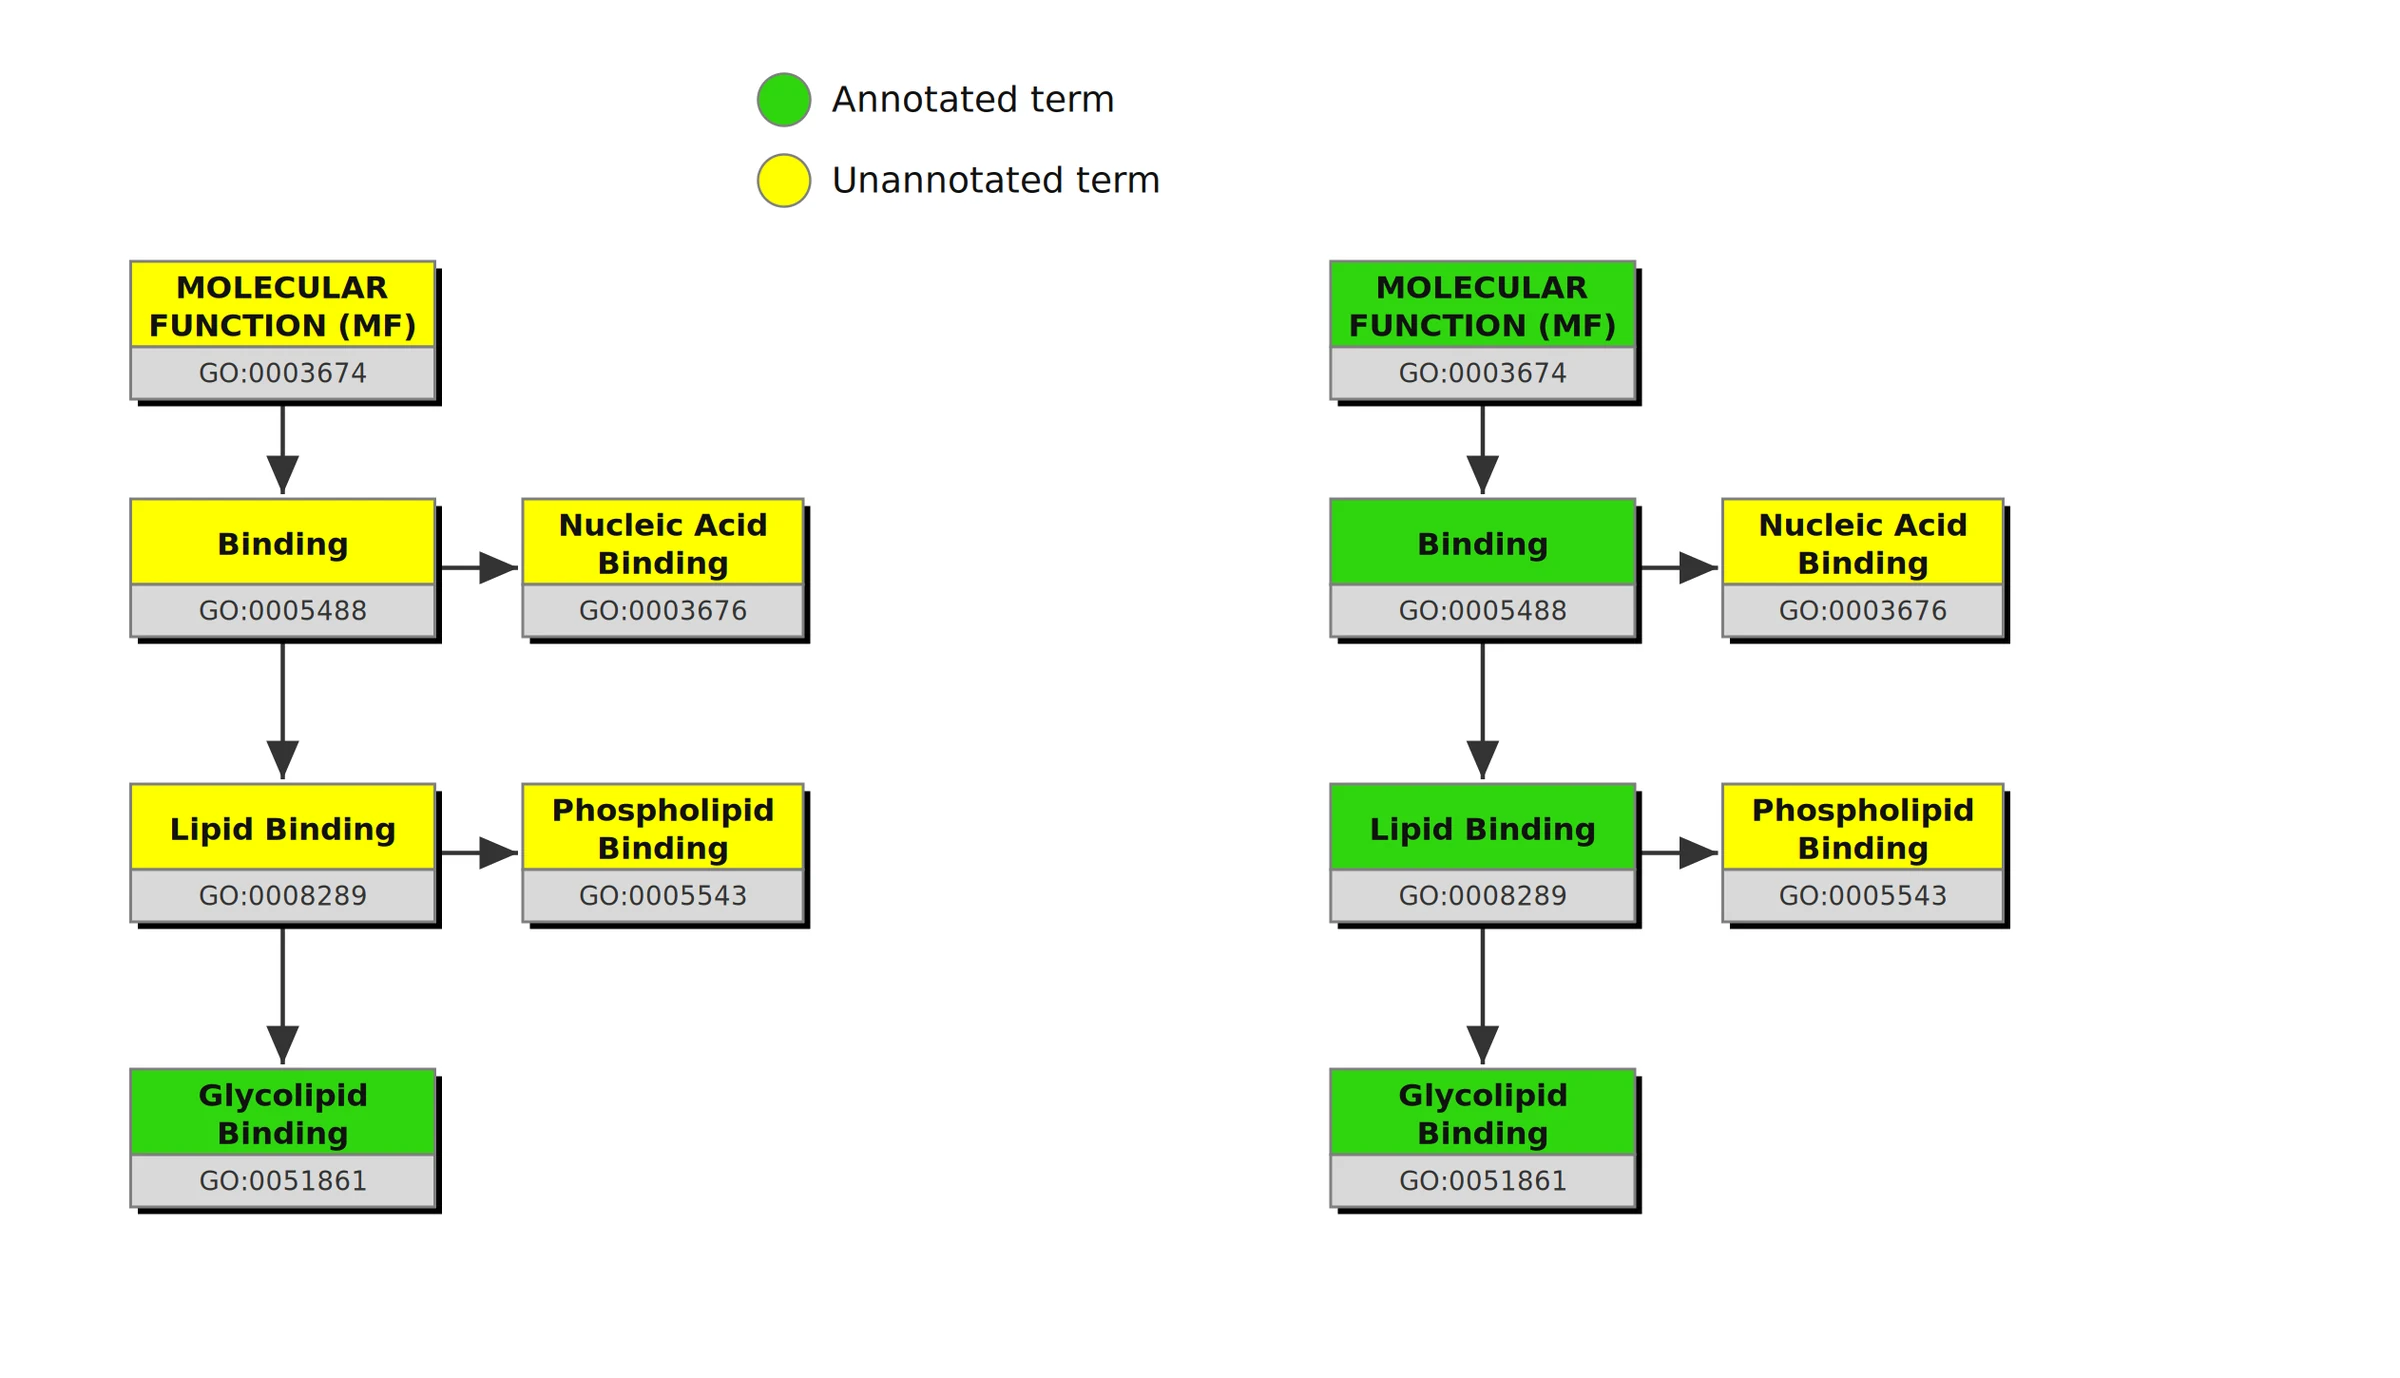
\includegraphics[width=775.3\px,height=445.2\px]{figures/fig_2_1.png}};
\fill<3>[plate] (1103.3,235) rectangle ++(387.7,445.2);
\node[tl] at (88,70) {\fmR\fz{16}{16}\color{inkii}\ls{2}\Ll{1 · Motivation}};
\node[tl] at (88,131) {\fdA\fz{54}{56.7}\color{ink}\ls{-1}\Ll{Function as a hierarchy of terms}};
\node<2-5>[tl] at (124,236) {\fbR\fz{30}{40.5}\color{ink}\Ll{Three ontologies: Biological Process\\(BP), Cellular Component (CC),\\Molecular Function (MF)}};
\node<3-5>[tl] at (124,379.5) {\fbR\fz{30}{40.5}\color{ink}\Ll{Each is a directed acyclic graph of terms\\({\fmR\fz{25.8}{31}{}is\_a}, {\fmR\fz{25.8}{31}{}part\_of})}};
\node<4-5>[tl] at (124,482.5) {\fbR\fz{30}{40.5}\color{ink}\Ll{True Path Rule: a term implies all\\its ancestors}};
\node<5>[tl] at (124,585.5) {\fbR\fz{30}{40.5}\color{ink}\Ll{Task: hierarchical multi-\\label classification}};
\node<3-5>[tl] at (694.7,718.2) {\fmR\fz{15}{19.5}\color{muted}\Ll{Dissertation, Fig. 2.1 · left inconsistent, right consistent}};
\node[tr] at (1512,876) {\fmR\fz{16}{16}\color{muted}4 / 45};
\end{tikzpicture}
\note{A protein carries many terms at different levels of specificity. If a specific term is annotated, every ancestor must be too. 

Predictions are made hierarchy-consistent before any metric is computed.}
\end{frame}

\begin{frame}[plain]
\begin{tikzpicture}[deck]
\node<1>[box] at (0,0) {\includegraphics[page=3,width=1600\px]{build/layers}};
\node<2>[box] at (0,0) {\includegraphics[page=11,width=1600\px]{build/layers}};
\node<3>[box] at (0,0) {\includegraphics[page=12,width=1600\px]{build/layers}};
\node<4>[box] at (0,0) {\includegraphics[page=13,width=1600\px]{build/layers}};
\node<2-4>[box] at (715.7,235) {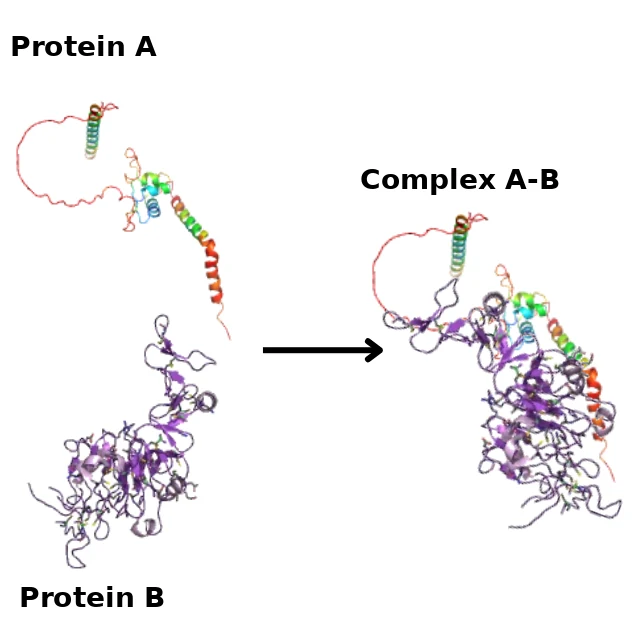
\includegraphics[width=223\px,height=223\px]{figures/fig_2_2.png}};
\node[tl] at (88,70) {\fmR\fz{16}{16}\color{inkii}\ls{2}\Ll{1 · Motivation}};
\node[tl] at (88,131) {\fdA\fz{54}{56.7}\color{ink}\ls{-1}\Ll{Function also depends on context}};
\node<2-4>[tl] at (124,236) {\fbR\fz{30}{40.5}\color{ink}\Ll{Proteins act in complexes and pathways}};
\node<2-4>[tl] at (124,298.5) {\fbR\fz{30}{40.5}\color{ink}\Ll{PPI networks: nodes are proteins, edges\\are associations}};
\node<3-4>[tl] at (124,401.5) {\fbR\fz{30}{40.5}\color{ink}\Ll{Guilt by association: connected proteins\\tend to share functions}};
\node<4>[tl] at (124,504.5) {\fbR\fz{30}{40.5}\color{ink}\Ll{But STRING mixes evidence of uneven\\reliability, and about one third of\\proteins have no edge}};
\node<2-4>[tl] at (694.7,496) {\fmR\fz{15}{19.5}\color{muted}\Ll{Dissertation, Fig. 2.2}};
\node[tr] at (1512,876) {\fmR\fz{16}{16}\color{muted}5 / 45};
\end{tikzpicture}
\note{Sequence-derived features are strong, but part of a protein's function is set by its cellular context. 

STRING aggregates experiments, curated databases, co-expression, genomic context and text mining into one confidence score. 

Coverage is uneven, which becomes the central limitation of a network-only model.}
\end{frame}

\begin{frame}[plain]
\begin{tikzpicture}[deck]
\node<1>[box] at (0,0) {\includegraphics[page=3,width=1600\px]{build/layers}};
\node<2>[box] at (0,0) {\includegraphics[page=14,width=1600\px]{build/layers}};
\node<3>[box] at (0,0) {\includegraphics[page=15,width=1600\px]{build/layers}};
\node<4>[box] at (0,0) {\includegraphics[page=16,width=1600\px]{build/layers}};
\node[tl] at (88,70) {\fmR\fz{16}{16}\color{inkii}\ls{2}\Ll{1 · Motivation}};
\node[tl] at (88,131) {\fdA\fz{54}{56.7}\color{ink}\ls{-1}\Ll{Seven research questions}};
\node<2-4>[tc] at (126,236) {\fmM\fz{20}{20}\color{ink}\Lc{RQ1}};
\node<2-4>[tl] at (184,236) {\fbR\fz{30}{39}\color{ink}\Ll{Which network representation works best?}};
\node<2-4>[tc] at (126,308) {\fmM\fz{20}{20}\color{ink}\Lc{RQ2}};
\node<2-4>[tl] at (184,308) {\fbR\fz{30}{39}\color{ink}\Ll{How much does propagating ProtT5 over\\STRING add?}};
\node<2-4>[tc] at (126,416) {\fmM\fz{20}{20}\color{ink}\Lc{RQ3}};
\node<2-4>[tl] at (184,416) {\fbR\fz{30}{39}\color{ink}\Ll{Fixed vs learned aggregation, vector vs\\image heads}};
\node<3-4>[tc] at (126,524) {\fmM\fz{20}{20}\color{ink}\Lc{RQ4}};
\node<3-4>[tl] at (184,524) {\fbR\fz{30}{39}\color{ink}\Ll{Do early and late fusion help?}};
\node<3-4>[tc] at (866,236) {\fmM\fz{20}{20}\color{ink}\Lc{RQ5}};
\node<3-4>[tl] at (924,236) {\fbR\fz{30}{39}\color{ink}\Ll{How deep, and how much retention?}};
\node<4>[tc] at (866,308) {\fmM\fz{20}{20}\color{ink}\Lc{RQ6}};
\node<4>[tl] at (924,308) {\fbR\fz{30}{39}\color{ink}\Ll{How does it compare with the literature?}};
\node<4>[tc] at (866,416) {\fmM\fz{20}{20}\color{ink}\Lc{RQ7}};
\node<4>[tl] at (924,416) {\fbR\fz{30}{39}\color{ink}\Ll{Does it work on one global, aggregated\\network?}};
\node[tr] at (1512,876) {\fmR\fz{16}{16}\color{muted}6 / 45};
\end{tikzpicture}
\note{Read the full questions from Section 1.3 only if asked. Each one is answered on the conclusions slide.}
\end{frame}

\begin{frame}[plain]
\begin{tikzpicture}[deck]
\node<1>[box] at (0,0) {\includegraphics[page=3,width=1600\px]{build/layers}};
\node<2>[box] at (0,0) {\includegraphics[page=17,width=1600\px]{build/layers}};
\node<3>[box] at (0,0) {\includegraphics[page=18,width=1600\px]{build/layers}};
\node<4>[box] at (0,0) {\includegraphics[page=19,width=1600\px]{build/layers}};
\node[tl] at (88,70) {\fmR\fz{16}{16}\color{inkii}\ls{2}\Ll{1 · Motivation}};
\node[tl] at (88,131) {\fdA\fz{54}{56.7}\color{ink}\ls{-1}\Ll{Contributions}};
\node<2-4>[tl] at (144,237) {\fbR\fz{32}{41.6}\color{ink}\Ll{NEXUS-GO: non-parametric multi-hop propagation of ProtT5 embeddings over STRING}};
\node<2-4>[tl] at (144,304.6) {\fbR\fz{32}{41.6}\color{ink}\Ll{Controlled comparison of fixed vs learned (GCN, GAT) aggregation}};
\node<2-4>[tl] at (144,372.2) {\fbR\fz{32}{41.6}\color{ink}\Ll{Vector vs image classification heads over the same embeddings}};
\node<3-4>[tl] at (144,439.8) {\fbR\fz{32}{41.6}\color{ink}\Ll{Early and late fusion of fixed and learned routes}};
\node<3-4>[tl] at (144,507.4) {\fbR\fz{32}{41.6}\color{ink}\Ll{Benchmark against five reimplemented methods, same splits and setting}};
\node<4>[tl] at (88,768.7) {\fmM\fz{18}{21.6}\color{ink}\Ll{VISAPP 2026 · published, pp. 157–166}};
\node<4>[tl] at (88,800.3) {\fbR\fz{21}{28.4}\color{inkii}\Ll{{\fbI\color{ink}{}From Graphs to Images: Non-Parametric PPI Context Integration for}\\{\fbI\color{ink}{}Vision-Based Protein Function Prediction}}};
\node<4>[tl] at (824,768.7) {\fmM\fz{18}{21.6}\color{ink}\Ll{CCIS · accepted, expected December 2026}};
\node<4>[tl] at (824,800.3) {\fbR\fz{21}{28.4}\color{inkii}\Ll{{\fbI\color{ink}{}Beyond Learnable Graphs: Fixed Multi-Hop PPI Diffusion of Sequence}\\{\fbI\color{ink}{}Embeddings for Robust Protein Function Prediction} · extended version}};
\node[tr] at (1512,876) {\fmR\fz{16}{16}\color{muted}7 / 45};
\end{tikzpicture}
\note{Five contributions, each answered with a result at the end. 

The first paper reported the first, sum-deduplicated campaign; the extended version continues the fixed route and adds a vector head next to the vision head. It was accepted in Communications in Computer and Information Science.}
\end{frame}

\section{2 · Background and related work}
\begin{frame}[plain]
\begin{tikzpicture}[deck]
\node<1>[box] at (0,0) {\includegraphics[page=3,width=1600\px]{build/layers}};
\node<2>[box] at (0,0) {\includegraphics[page=20,width=1600\px]{build/layers}};
\node<3>[box] at (0,0) {\includegraphics[page=21,width=1600\px]{build/layers}};
\node<4>[box] at (0,0) {\includegraphics[page=22,width=1600\px]{build/layers}};
\node<5>[box] at (0,0) {\includegraphics[page=23,width=1600\px]{build/layers}};
\node<2-5>[box] at (123.6,235) {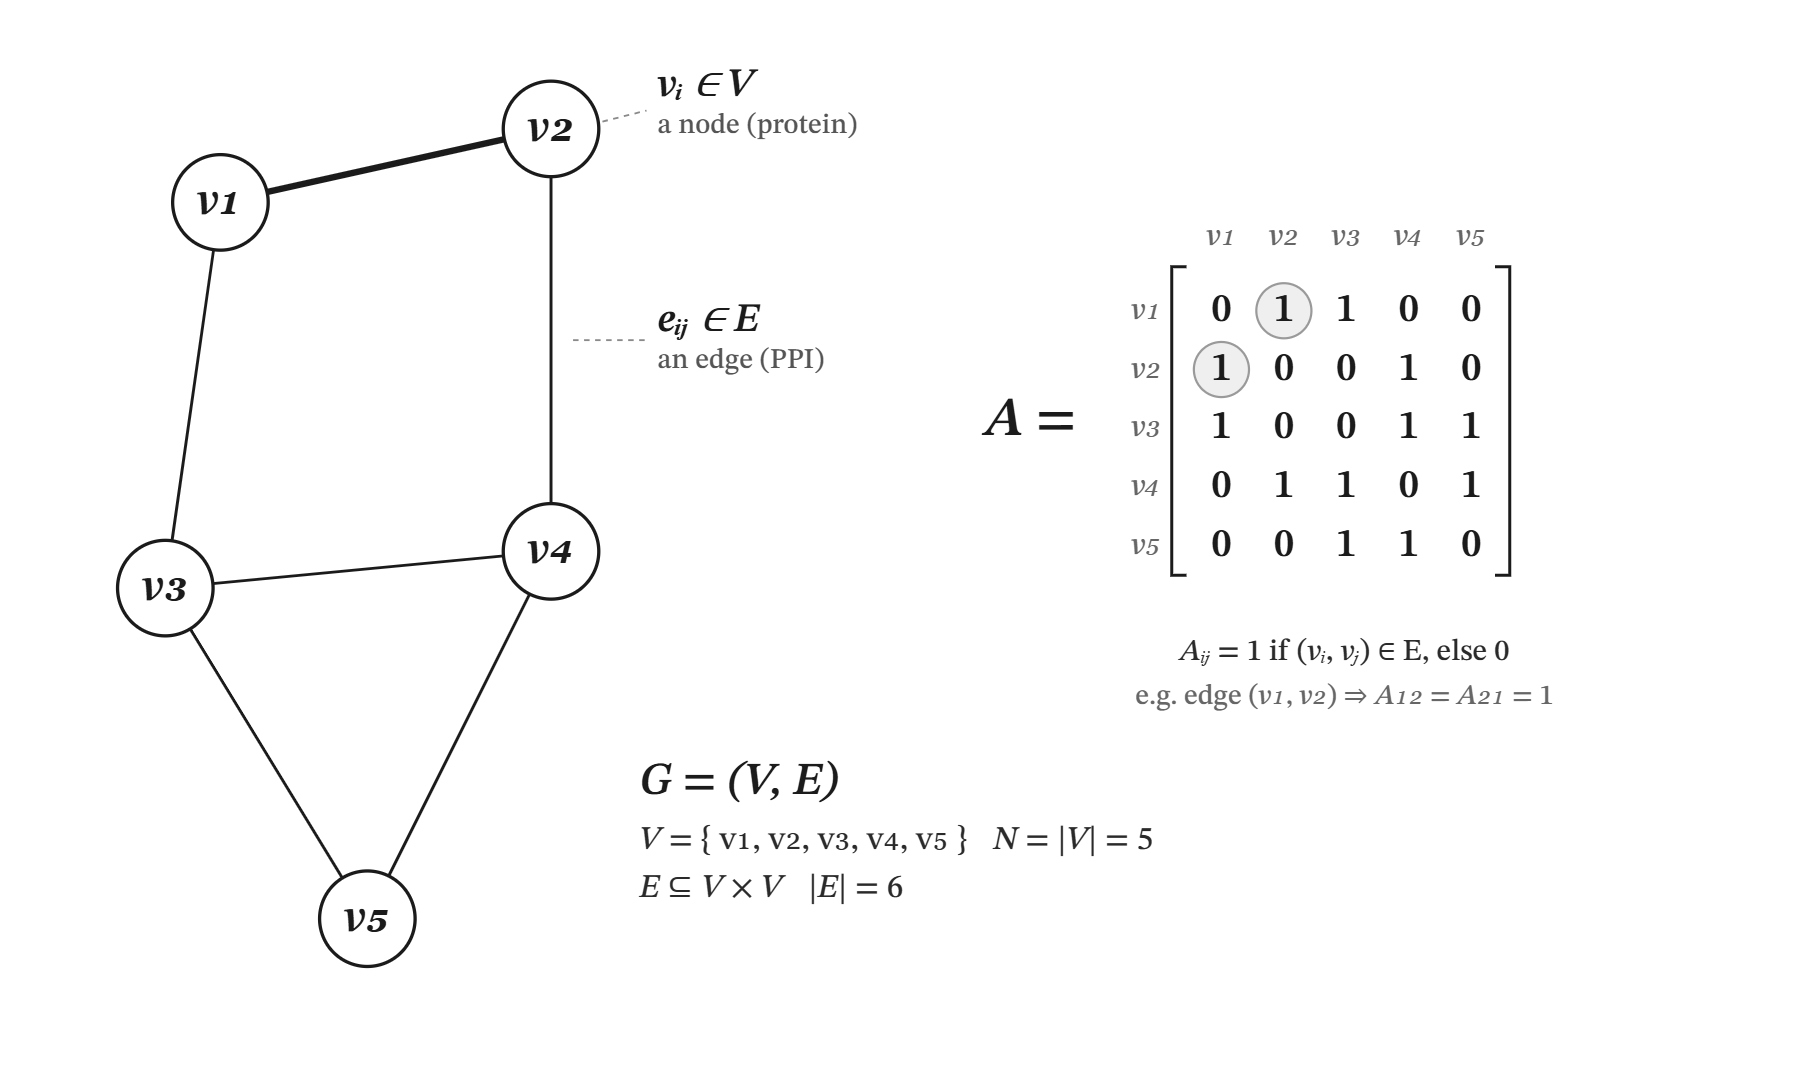
\includegraphics[width=624.8\px,height=370\px]{figures/fig_2_3.png}};
\node[tl] at (88,70) {\fmR\fz{16}{16}\color{inkii}\ls{2}\Ll{2 · Background and related work}};
\node[tl] at (88,131) {\fdA\fz{54}{56.7}\color{ink}\ls{-1}\Ll{Graphs, adjacency and message passing}};
\node<2-5>[tl] at (88,643) {\fmR\fz{15}{19.5}\color{muted}\Ll{Dissertation, Fig. 2.3}};
\node<2-5>[tl] at (124,689) {\fbR\fz{26}{35.1}\color{ink}\Ll{{\fz{29.2}{35}$G = (V, E, w)$}: proteins, associations,\\STRING confidence}};
\node<3-5>[tl] at (852,689) {\fbR\fz{26}{35.1}\color{ink}\Ll{Message passing: aggregate neighbours, update\\the node}};
\node<2-5>[tl] at (124,775.2) {\fbR\fz{26}{35.1}\color{ink}\Ll{Adjacency matrix {\fz{29.2}{35}$A$}; sparse storage {\fz{29.2}{35}$O(|E|)$}}};
\node<5>[tl] at (852,775.2) {\fbR\fz{26}{35.1}\color{ink}\Ll{{\fz{29.2}{35}$L$} layers reach {\fz{29.2}{35}$L$} hops; too many cause oversmoothing}};
\node[tr] at (1512,876) {\fmR\fz{16}{16}\color{muted}8 / 45};
\end{tikzpicture}
\note{GCN aggregates with a symmetrically normalized adjacency; GAT learns attention weights over neighbours. 

Each layer widens the receptive field by one hop, and too many layers make neighbouring representations indistinguishable.}
\end{frame}

\begin{frame}[plain]
\begin{tikzpicture}[deck]
\node<1>[box] at (0,0) {\includegraphics[page=3,width=1600\px]{build/layers}};
\node<2>[box] at (0,0) {\includegraphics[page=24,width=1600\px]{build/layers}};
\node<3>[box] at (0,0) {\includegraphics[page=25,width=1600\px]{build/layers}};
\node<4>[box] at (0,0) {\includegraphics[page=26,width=1600\px]{build/layers}};
\node<3-4>[box] at (594.3,440) {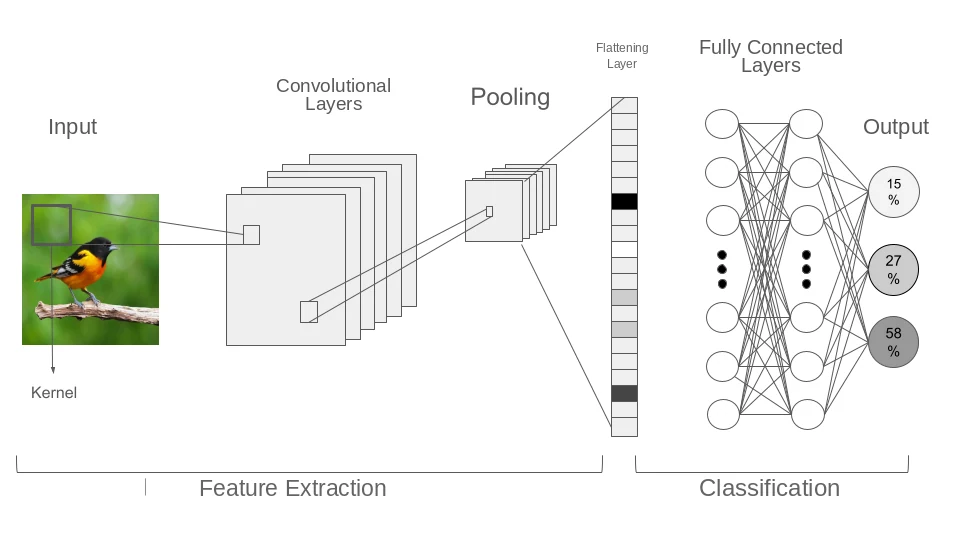
\includegraphics[width=411.3\px,height=231.4\px]{figures/fig_2_6.png}};
\node<4>[box] at (1079.7,435.7) {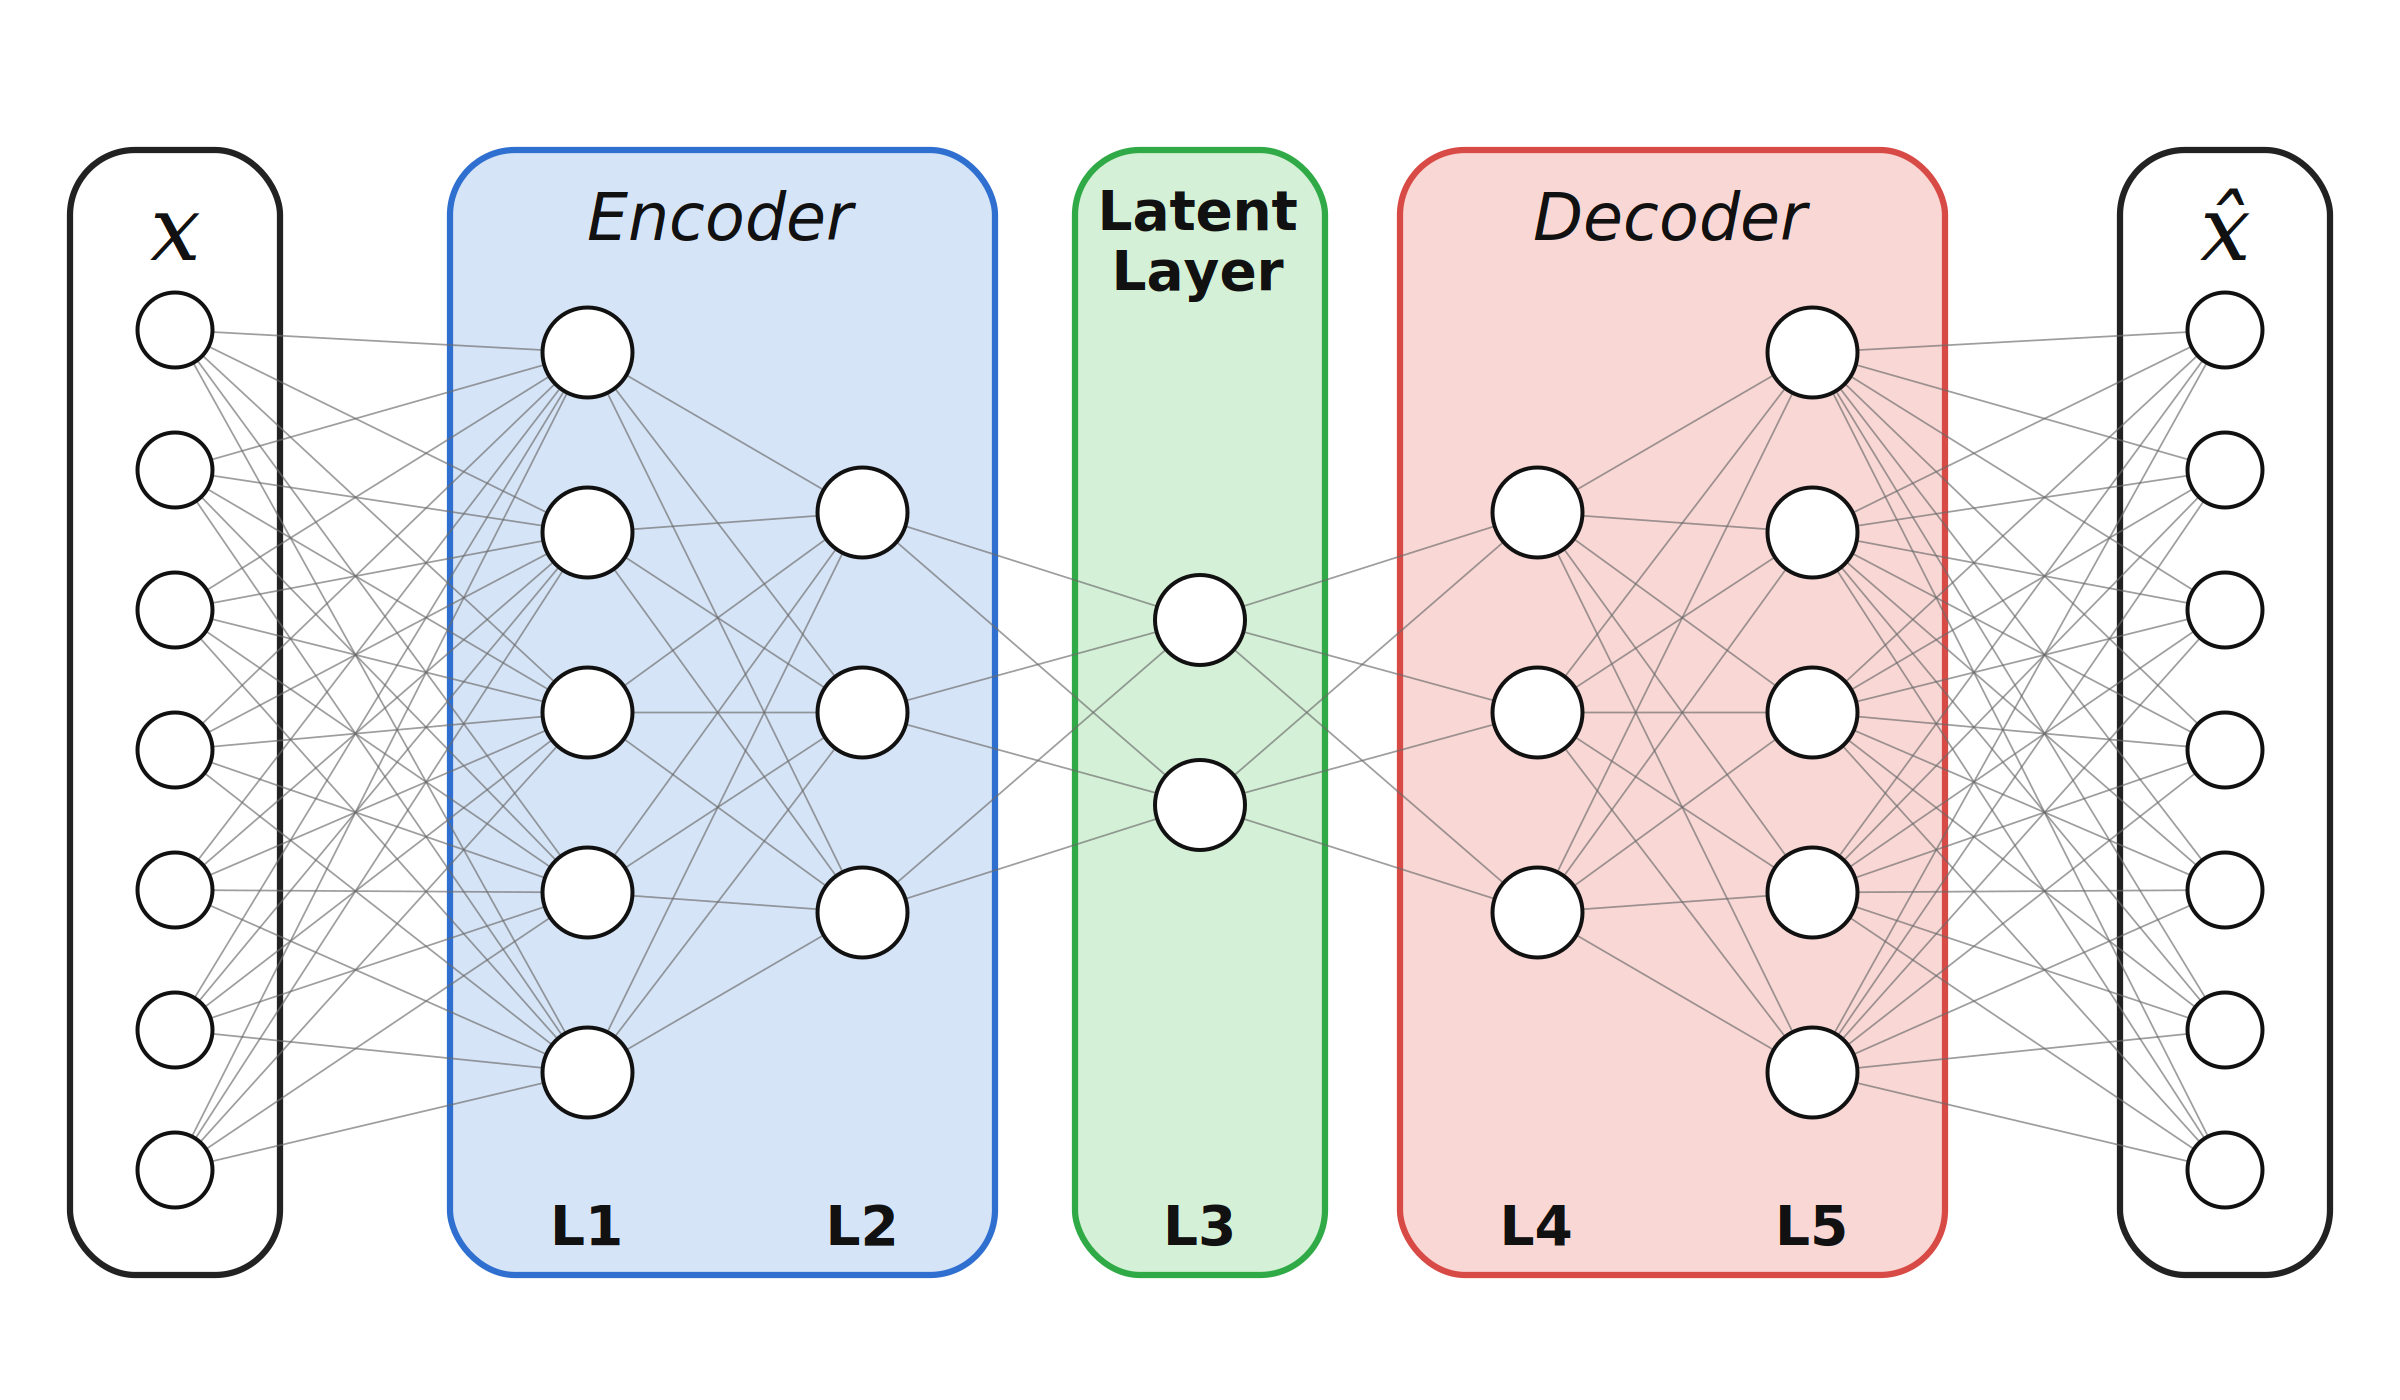
\includegraphics[width=411.3\px,height=239.9\px]{figures/fig_2_7.png}};
\node[tl] at (88,70) {\fmR\fz{16}{16}\color{inkii}\ls{2}\Ll{2 · Background and related work}};
\node[tl] at (88,131) {\fdA\fz{54}{56.7}\color{ink}\ls{-1}\Ll{Building blocks}};
\node<2-4>[tl] at (88,230) {\fbR\fz{24}{32.4}\color{ink}\Ll{{\fbB{}MLP}: the vector prediction head}};
\node<3-4>[tl] at (573.3,230) {\fbR\fz{24}{32.4}\color{ink}\Ll{{\fbB{}CNN}: the backbone of the image route\\(ResNet-50, ConvNeXt-Tiny)}};
\node<4>[tl] at (1058.7,230) {\fbR\fz{24}{32.4}\color{ink}\Ll{{\fbB{}Autoencoder}: the compression inside\\deepNF, one of the baselines}};
\node<2-4>[tl] at (88,854.9) {\fmR\fz{15}{19.5}\color{muted}\Ll{Dissertation, Figs. 2.4 and 2.5}};
\node<3-4>[tl] at (573.3,831.5) {\fmR\fz{15}{19.5}\color{muted}\Ll{Dissertation, Fig. 2.6}};
\node<4>[tl] at (1058.7,831.5) {\fmR\fz{15}{19.5}\color{muted}\Ll{Dissertation, Fig. 2.7}};
\node[tr] at (1512,876) {\fmR\fz{16}{16}\color{muted}9 / 45};
\end{tikzpicture}
\note{Only what the rest of the talk needs. 

The MLP is the vector head, the CNN is the vision head, and the autoencoder is how deepNF compresses diffusion states.}
\end{frame}

\begin{frame}[plain]
\begin{tikzpicture}[deck]
\node<1>[box] at (0,0) {\includegraphics[page=3,width=1600\px]{build/layers}};
\node<2>[box] at (0,0) {\includegraphics[page=27,width=1600\px]{build/layers}};
\node<3>[box] at (0,0) {\includegraphics[page=28,width=1600\px]{build/layers}};
\node<4>[box] at (0,0) {\includegraphics[page=29,width=1600\px]{build/layers}};
\node<5>[box] at (0,0) {\includegraphics[page=30,width=1600\px]{build/layers}};
\node[tl] at (88,70) {\fmR\fz{16}{16}\color{inkii}\ls{2}\Ll{2 · Background and related work}};
\node[tl] at (88,131) {\fdA\fz{54}{56.7}\color{ink}\ls{-1}\Ll{Protein language models}};
\node<2-5>[tl] at (124,236) {\fbR\fz{30}{40.5}\color{ink}\Ll{Self-supervised pretraining on hundreds\\of millions of sequences}};
\node<3-5>[tl] at (124,339) {\fbR\fz{30}{40.5}\color{ink}\Ll{Transformer encoder: every residue\\attends to every other}};
\node<4-5>[tl] at (124,442) {\fbR\fz{30}{40.5}\color{ink}\Ll{ProtT5-XL-U50: T5 encoder, BFD then\\UniRef50, 15\% residue masking}};
\node<5>[tl] at (124,545) {\fbR\fz{30}{40.5}\color{ink}\Ll{Used here as a frozen feature extractor}};
\node[tr] at (1512,876) {\fmR\fz{16}{16}\color{muted}10 / 45};
\end{tikzpicture}
\note{Language models turn function prediction into ordinary multi-label classification over a fixed-length vector. 

No gradient from our task reaches ProtT5; we read three encoder layers and keep them fixed.}
\end{frame}

\begin{frame}[plain]
\begin{tikzpicture}[deck]
\node<1>[box] at (0,0) {\includegraphics[page=3,width=1600\px]{build/layers}};
\node<2>[box] at (0,0) {\includegraphics[page=31,width=1600\px]{build/layers}};
\node<3>[box] at (0,0) {\includegraphics[page=32,width=1600\px]{build/layers}};
\node<4>[box] at (0,0) {\includegraphics[page=33,width=1600\px]{build/layers}};
\node[tl] at (88,70) {\fmR\fz{16}{16}\color{inkii}\ls{2}\Ll{2 · Background and related work}};
\node[tl] at (88,131) {\fdA\fz{54}{56.7}\color{ink}\ls{-1}\Ll{From neighbour voting to graph transformers}};
\node[tr] at (1512,876) {\fmR\fz{16}{16}\color{muted}11 / 45};
\end{tikzpicture}
\note{The field moved from fixed diffusion to learned attention, and each step added parameters. 

Decoupled methods such as SGC and APPNP move against that trend, and SEGT-GO's multi-hop aggregation is itself a plain matrix product.}
\end{frame}

\begin{frame}[plain]
\begin{tikzpicture}[deck]
\node<1-2>[box] at (0,0) {\includegraphics[page=3,width=1600\px]{build/layers}};
\node<3>[box] at (0,0) {\includegraphics[page=34,width=1600\px]{build/layers}};
\node<4>[box] at (0,0) {\includegraphics[page=35,width=1600\px]{build/layers}};
\node<5>[box] at (0,0) {\includegraphics[page=36,width=1600\px]{build/layers}};
\node[tl] at (88,70) {\fmR\fz{16}{16}\color{inkii}\ls{2}\Ll{2 · Background and related work}};
\node[tl] at (88,131) {\fdA\fz{54}{56.7}\color{ink}\ls{-1}\Ll{The open question}};
\node<2-5>[tl] at (88,262) {\fdA\fz{64}{69.1}\color{ink}\ls{-1.5}\Ll{Is a learned graph component still needed\\once the propagated object is informative?}};
\node<3-5>[tl] at (124,426.2) {\fbR\fz{30}{40.5}\color{ink}\Ll{Proposal: propagate ProtT5 embeddings with a fixed, finite-step operator, then use an\\ordinary head}};
\node<4-5>[tl] at (124,529.2) {\fbR\fz{30}{40.5}\color{ink}\Ll{A sequence representation exists for every protein, so the network adds instead\\of supplies}};
\node<5>[tl] at (124,632.2) {\fbR\fz{30}{40.5}\color{ink}\Ll{No prior visual route starts from a propagated language-model embedding}};
\node[tr] at (1512,876) {\fmR\fz{16}{16}\color{muted}12 / 45};
\end{tikzpicture}
\note{The contribution is an architectural placement, not a new propagation mechanism. 

To our knowledge no previous work propagates protein language model embeddings directly while simplifying what consumes them.}
\end{frame}

\section{3 · Data and evaluation}
\begin{frame}[plain]
\begin{tikzpicture}[deck]
\node<1>[box] at (0,0) {\includegraphics[page=3,width=1600\px]{build/layers}};
\node<2>[box] at (0,0) {\includegraphics[page=37,width=1600\px]{build/layers}};
\node<3>[box] at (0,0) {\includegraphics[page=38,width=1600\px]{build/layers}};
\node<4>[box] at (0,0) {\includegraphics[page=39,width=1600\px]{build/layers}};
\node[tl] at (88,70) {\fmR\fz{16}{16}\color{inkii}\ls{2}\Ll{3 · Data and evaluation}};
\node[tl] at (88,131) {\fdA\fz{54}{56.7}\color{ink}\ls{-1}\Ll{Data: a CAFA5-derived corpus}};
\node<2-4>[tl] at (106,237) {\fbB\fz{20}{24}\color{inkii}\Ll{Ontology}};
\node<2-4>[tr] at (547.6,237) {\fbB\fz{20}{24}\color{inkii}\Lr{Training}};
\node<2-4>[tr] at (677.8,237) {\fbB\fz{20}{24}\color{inkii}\Lr{Validation}};
\node<2-4>[tr] at (797.8,237) {\fbB\fz{20}{24}\color{inkii}\Lr{Test}};
\node<2-4>[tr] at (891.1,237) {\fbB\fz{20}{24}\color{inkii}\Lr{Terms}};
\node<2-4>[tl] at (106,295) {\fbR\fz{28}{33.6}\color{ink}\Ll{Biological Process (BP)}};
\node<2-4>[tr] at (547.6,296) {\fmR\fz{28}{33.6}\color{ink}\Lr{73,768}};
\node<2-4>[tr] at (677.8,296) {\fmR\fz{28}{33.6}\color{ink}\Lr{9,221}};
\node<2-4>[tr] at (797.8,296) {\fmR\fz{28}{33.6}\color{ink}\Lr{9,221}};
\node<2-4>[tr] at (891.1,296) {\fmR\fz{28}{33.6}\color{ink}\Lr{500}};
\node<2-4>[tl] at (106,357) {\fbR\fz{28}{33.6}\color{ink}\Ll{Cellular Component (CC)}};
\node<2-4>[tr] at (547.6,358) {\fmR\fz{28}{33.6}\color{ink}\Lr{74,328}};
\node<2-4>[tr] at (677.8,358) {\fmR\fz{28}{33.6}\color{ink}\Lr{9,292}};
\node<2-4>[tr] at (797.8,358) {\fmR\fz{28}{33.6}\color{ink}\Lr{9,292}};
\node<2-4>[tr] at (891.1,358) {\fmR\fz{28}{33.6}\color{ink}\Lr{498}};
\node<2-4>[tl] at (106,419) {\fbR\fz{28}{33.6}\color{ink}\Ll{Molecular Function (MF)}};
\node<2-4>[tr] at (547.6,420) {\fmR\fz{28}{33.6}\color{ink}\Lr{62,909}};
\node<2-4>[tr] at (677.8,420) {\fmR\fz{28}{33.6}\color{ink}\Lr{7,864}};
\node<2-4>[tr] at (797.8,420) {\fmR\fz{28}{33.6}\color{ink}\Lr{7,864}};
\node<2-4>[tr] at (891.1,420) {\fmR\fz{28}{33.6}\color{ink}\Lr{499}};
\node<2-4>[tl] at (88,466) {\fmR\fz{15}{19.5}\color{muted}\Ll{Dissertation, Table 4.1}};
\node<3-4>[tl] at (973.3,236) {\fbR\fz{30}{40.5}\color{ink}\Ll{80 / 10 / 10 split, disjoint at\\protein level, no temporal or\\homology constraint}};
\node<4>[tl] at (973.3,379.5) {\fbR\fz{30}{40.5}\color{ink}\Ll{Labels per protein (mean): 25.91 BP,\\12.48 CC, 7.55 MF}};
\node<4>[tl] at (973.3,482.5) {\fbR\fz{30}{40.5}\color{ink}\Ll{Label matrix density:}};
\node<4>[tl] at (973.3,526) {\fmR\fz{22}{29.7}\color{inkii}\Ll{BP}};
\node<4>[tl] at (1164,526) {\fmR\fz{22}{29.7}\color{ink}\Ll{5.18\%}};
\node<4>[tl] at (973.3,565.7) {\fmR\fz{22}{29.7}\color{inkii}\Ll{CC}};
\node<4>[tl] at (1094.6,565.7) {\fmR\fz{22}{29.7}\color{ink}\Ll{2.51\%}};
\node<4>[tl] at (973.3,605.4) {\fmR\fz{22}{29.7}\color{inkii}\Ll{MF}};
\node<4>[tl] at (1068.6,605.4) {\fmR\fz{22}{29.7}\color{ink}\Ll{1.51\%}};
\node[tr] at (1512,876) {\fmR\fz{16}{16}\color{muted}13 / 45};
\end{tikzpicture}
\note{The official CAFA5 test labels were not available, so the splits come from the training corpus. 

Only about five hundred most frequent terms per ontology are kept, which makes absolute values not comparable with CAFA numbers.}
\end{frame}

\begin{frame}[plain]
\begin{tikzpicture}[deck]
\node<1>[box] at (0,0) {\includegraphics[page=3,width=1600\px]{build/layers}};
\node<2>[box] at (0,0) {\includegraphics[page=40,width=1600\px]{build/layers}};
\node<3>[box] at (0,0) {\includegraphics[page=41,width=1600\px]{build/layers}};
\node<4>[box] at (0,0) {\includegraphics[page=42,width=1600\px]{build/layers}};
\node<2-4>[box] at (109,235) {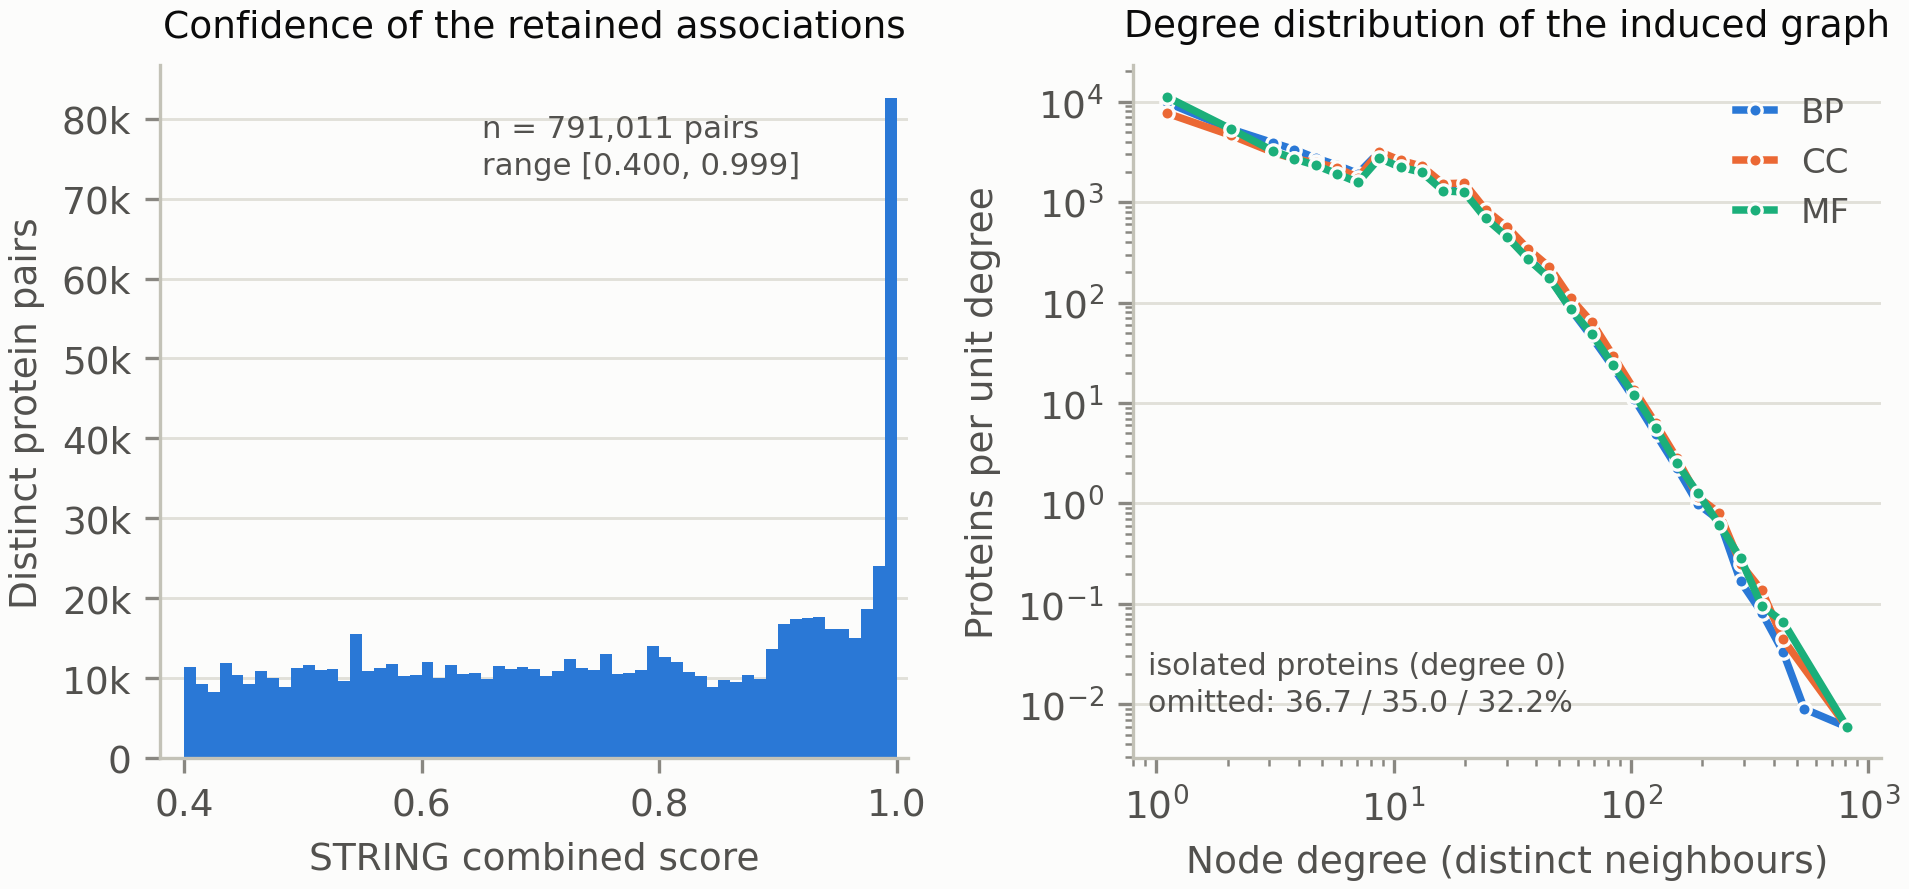
\includegraphics[width=775.3\px,height=361\px]{figures/fig_4_1.png}};
\fill<2-3>[plate] (496.7,235) rectangle ++(387.7,361);
\node[tl] at (88,70) {\fmR\fz{16}{16}\color{inkii}\ls{2}\Ll{3 · Data and evaluation}};
\node[tl] at (88,131) {\fdA\fz{54}{56.7}\color{ink}\ls{-1}\Ll{STRING v11.5: one aggregated network}};
\node<2-4>[tl] at (88,634) {\fmR\fz{15}{19.5}\color{muted}\Ll{Dissertation, Fig. 4.1 · left combined score, right degree}};
\node<2-4>[tl] at (973.3,232) {\fbR\fz{26}{35.1}\color{ink}\Ll{2,422,234 records, 791,011 distinct pairs,\\86,423 proteins}};
\node<2-4>[tl] at (973.3,318.2) {\fbR\fz{26}{35.1}\color{ink}\Ll{Combined score in [0.400, 0.999]; confidence,\\not binding strength}};
\node<3-4>[tl] at (973.3,404.4) {\fbR\fz{26}{35.1}\color{ink}\Ll{Each pair repeated 3.06 times on average (up\\to 170), always with the same score}};
\node<4>[tl] at (973.3,490.6) {\fbR\fz{26}{35.1}\color{ink}\Ll{Degree is heavy-tailed: median 5 to 7,\\maximum 763 to 805}};
\node[tr] at (1512,876) {\fmR\fz{16}{16}\color{muted}14 / 45};
\end{tikzpicture}
\note{The medium-confidence floor of 400 comes with the inherited file. 

Repeated records carry no extra score information, which later decides the deduplication rule. Some knowledge circularity with the annotations cannot be excluded.}
\end{frame}

\begin{frame}[plain]
\begin{tikzpicture}[deck]
\node<1>[box] at (0,0) {\includegraphics[page=3,width=1600\px]{build/layers}};
\node<2>[box] at (0,0) {\includegraphics[page=43,width=1600\px]{build/layers}};
\node<3>[box] at (0,0) {\includegraphics[page=44,width=1600\px]{build/layers}};
\node<2-3>[box] at (109,235.6) {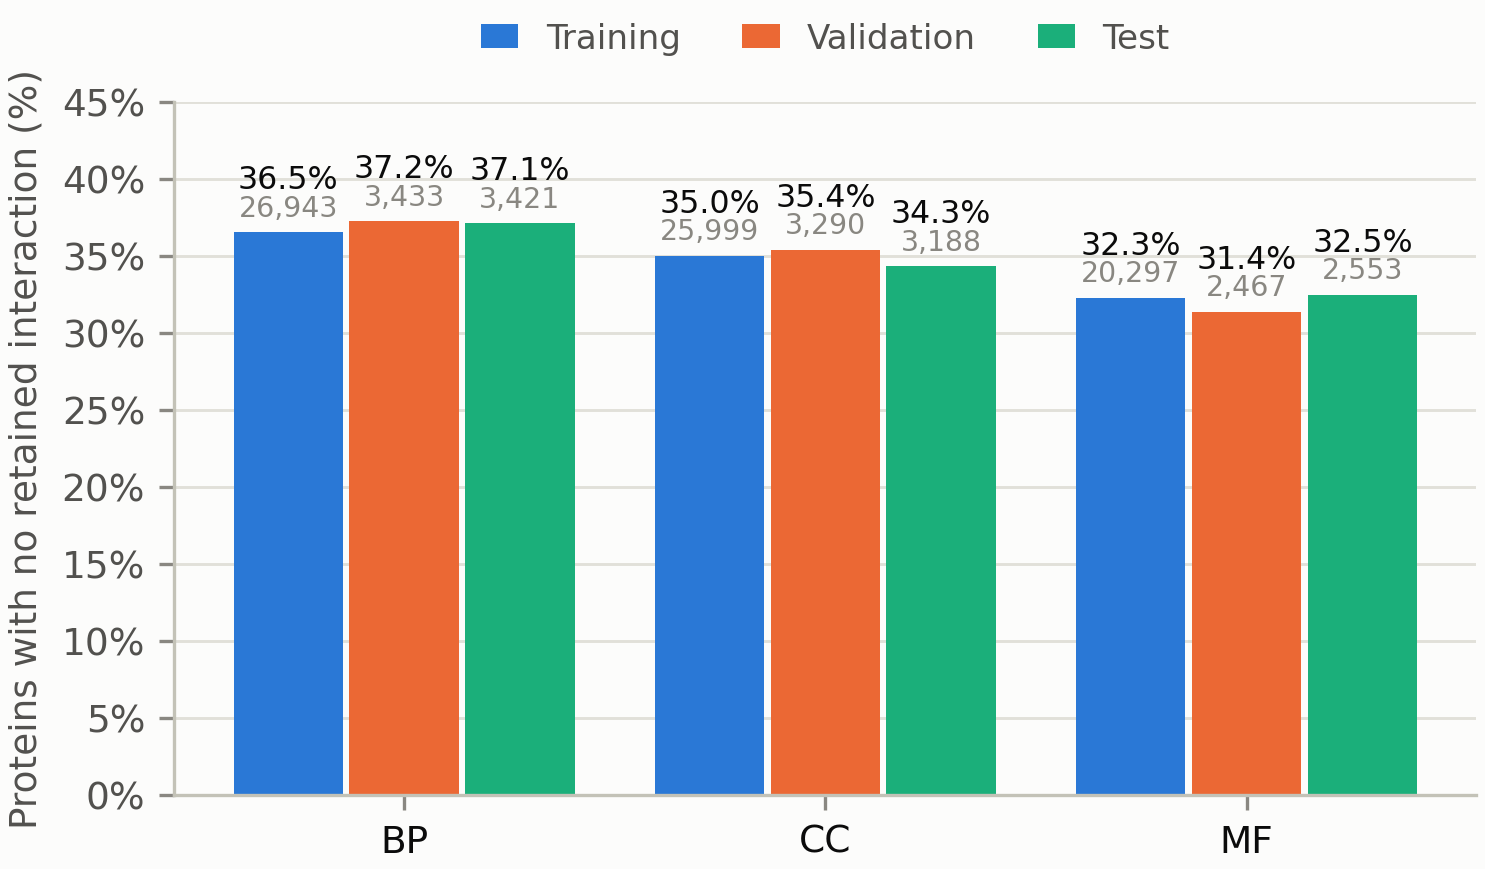
\includegraphics[width=654\px,height=382.7\px]{figures/fig_4_2.png}};
\node<3>[box] at (843.3,235) {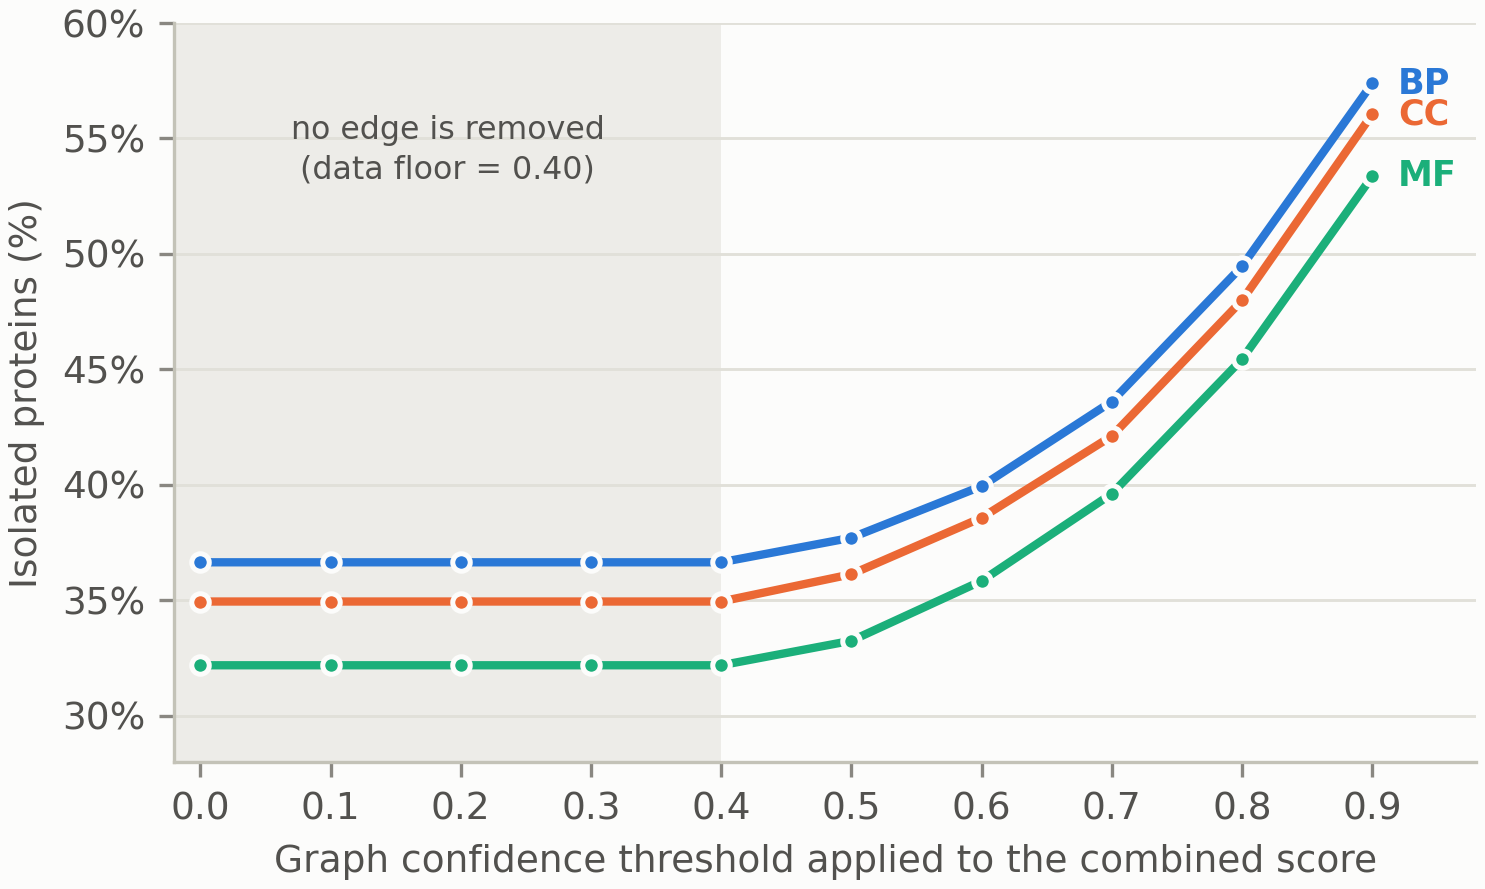
\includegraphics[width=641.4\px,height=384\px]{figures/fig_4_3.png}};
\node[tl] at (88,70) {\fmR\fz{16}{16}\color{inkii}\ls{2}\Ll{3 · Data and evaluation}};
\node[tl] at (88,131) {\fdA\fz{54}{56.7}\color{ink}\ls{-1}\Ll{One third of the proteins have no edge}};
\node<2-3>[tl] at (88,657) {\fmR\fz{15}{19.5}\color{muted}\Ll{Dissertation, Fig. 4.2}};
\node<2-3>[tl] at (124,719.5) {\fbR\fz{30}{40.5}\color{ink}\Ll{Isolated: 36.65\% BP, 34.95\% CC, 32.19\% MF}};
\node<2-3>[tl] at (124,782) {\fbR\fz{30}{40.5}\color{ink}\Ll{Stable across training, validation and test}};
\node<3>[tl] at (816,657) {\fmR\fz{15}{19.5}\color{muted}\Ll{Dissertation, Fig. 4.3}};
\node<3>[tl] at (852,719.5) {\fbR\fz{30}{40.5}\color{ink}\Ll{Thresholds up to 0.40 are inert; at 0.90 more\\than half the proteins are isolated}};
\node[tr] at (1512,876) {\fmR\fz{16}{16}\color{muted}15 / 45};
\end{tikzpicture}
\note{Isolated proteins were kept as nodes so that every protein is scored. For a model that sees only the network, these proteins have no input at all. 

This is the limitation the second generation is built to remove.}
\end{frame}

\begin{frame}[plain]
\begin{tikzpicture}[deck]
\node<1>[box] at (0,0) {\includegraphics[page=3,width=1600\px]{build/layers}};
\node<2>[box] at (0,0) {\includegraphics[page=7,width=1600\px]{build/layers}};
\node<3>[box] at (0,0) {\includegraphics[page=45,width=1600\px]{build/layers}};
\node<4>[box] at (0,0) {\includegraphics[page=46,width=1600\px]{build/layers}};
\node[tl] at (88,70) {\fmR\fz{16}{16}\color{inkii}\ls{2}\Ll{3 · Data and evaluation}};
\node[tl] at (88,131) {\fdA\fz{54}{56.7}\color{ink}\ls{-1}\Ll{Six protein-centric metrics}};
\node<2-4>[tl] at (124,236) {\fbR\fz{30}{40.5}\color{ink}\Ll{Primary criterion: wF\textsubscript{max}, information-\\content weighted}};
\node<3-4>[tl] at (124,339) {\fbR\fz{30}{40.5}\color{ink}\Ll{Also F\textsubscript{max}, F*\textsubscript{max} (root excluded), S\textsubscript{min}\\(bits, lower is better), AuPRC, IAuPRC}};
\node<4>[tl] at (124,442) {\fbR\fz{30}{40.5}\color{ink}\Ll{Predictions made hierarchy-consistent\\before scoring}};
\node<4>[tl] at (124,545) {\fbR\fz{30}{40.5}\color{ink}\Ll{101 thresholds; full evaluation mode\\(unpredicted proteins count as\\zero recall)}};
\node<2-4>[tl] at (694.7,261.7) {\fbR\fz{34}{40.8}\color{ink}\Ll{{\fz{38.2}{45.8}$\displaystyle wF_{\max} = \max_{\tau}\, \frac{2 \cdot wpr(\tau) \cdot wrc(\tau)}{wpr(\tau) + wrc(\tau)}$}}};
\node<2-4>[tl] at (694.7,341.4) {\fbR\fz{24}{32.4}\color{inkii}\Ll{each term weighted by its information content, {\fz{26.9}{32.3}$\mathrm{IC}(v) = -\log_2 \widehat{P}\bigl(v \mid \mathrm{pa}(v)\bigr)$}}};
\node<4>[tl] at (694.7,409.5) {\fbR\fz{34}{40.8}\color{ink}\Ll{{\fz{38.2}{45.8}$\displaystyle \tilde{s}_{iv} = \max_{u \in \mathcal{D}(v)} s_{iu}$}}};
\node[tr] at (1512,876) {\fmR\fz{16}{16}\color{muted}16 / 45};
\end{tikzpicture}
\note{wF\textsubscript{max} weights each term by information content, so frequent terms near the root count little. It is the selection criterion everywhere. 

The ancestor closure of predictions uses \texttt{is\_a} only, which matters most for CC.}
\end{frame}

\begin{frame}[plain]
\begin{tikzpicture}[deck]
\node<1>[box] at (0,0) {\includegraphics[page=3,width=1600\px]{build/layers}};
\node<2>[box] at (0,0) {\includegraphics[page=47,width=1600\px]{build/layers}};
\node<3>[box] at (0,0) {\includegraphics[page=48,width=1600\px]{build/layers}};
\node<4>[box] at (0,0) {\includegraphics[page=49,width=1600\px]{build/layers}};
\node<2-4>[box] at (109,235) {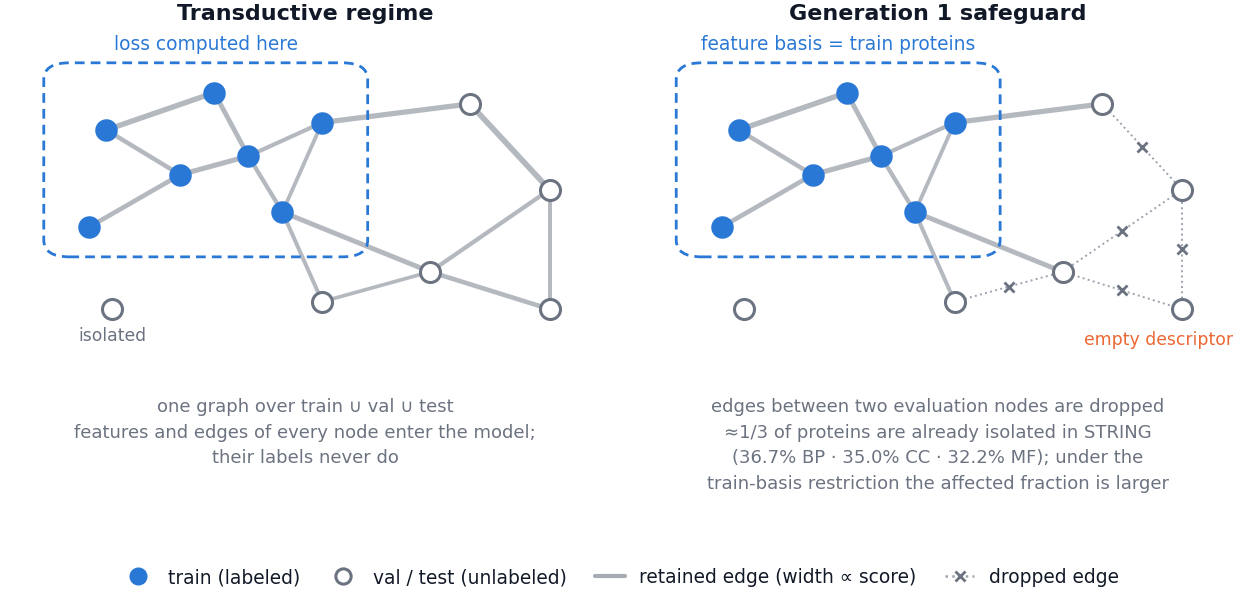
\includegraphics[width=775.3\px,height=373.3\px]{figures/fig_5_2.png}};
\node[tl] at (88,70) {\fmR\fz{16}{16}\color{inkii}\ls{2}\Ll{3 · Data and evaluation}};
\node[tl] at (88,131) {\fdA\fz{54}{56.7}\color{ink}\ls{-1}\Ll{Learning regime and protocol}};
\node<2-4>[tl] at (88,646.3) {\fmR\fz{15}{19.5}\color{muted}\Ll{Dissertation, Fig. 5.2}};
\node<2-4>[tl] at (973.3,232) {\fbR\fz{26}{35.1}\color{ink}\Ll{One graph over train $\cup$ validation $\cup$ test; labels\\read only for training proteins}};
\node<3-4>[tl] at (973.3,318.2) {\fbR\fz{26}{35.1}\color{ink}\Ll{Every design decision on validation; test\\read once}};
\node<4>[tl] at (973.3,404.4) {\fbR\fz{26}{35.1}\color{ink}\Ll{Single seed: differences below 0.5 pp are ties\\(interpretability floor)}};
\node[tr] at (1512,876) {\fmR\fz{16}{16}\color{muted}17 / 45};
\end{tikzpicture}
\note{Validation and test proteins contribute features and edges but never labels. The first generation uses a stricter train-basis construction. 

With a single seed, the talk treats sub-0.5 pp gaps as ties.}
\end{frame}

\section{4 · Method}
\begin{frame}[plain]
\begin{tikzpicture}[deck]
\node<1>[box] at (0,0) {\includegraphics[page=3,width=1600\px]{build/layers}};
\node<2>[box] at (0,0) {\includegraphics[page=50,width=1600\px]{build/layers}};
\node<3-4>[box] at (0,0) {\includegraphics[page=51,width=1600\px]{build/layers}};
\node<5>[box] at (0,0) {\includegraphics[page=52,width=1600\px]{build/layers}};
\node<2-5>[box] at (109,235) {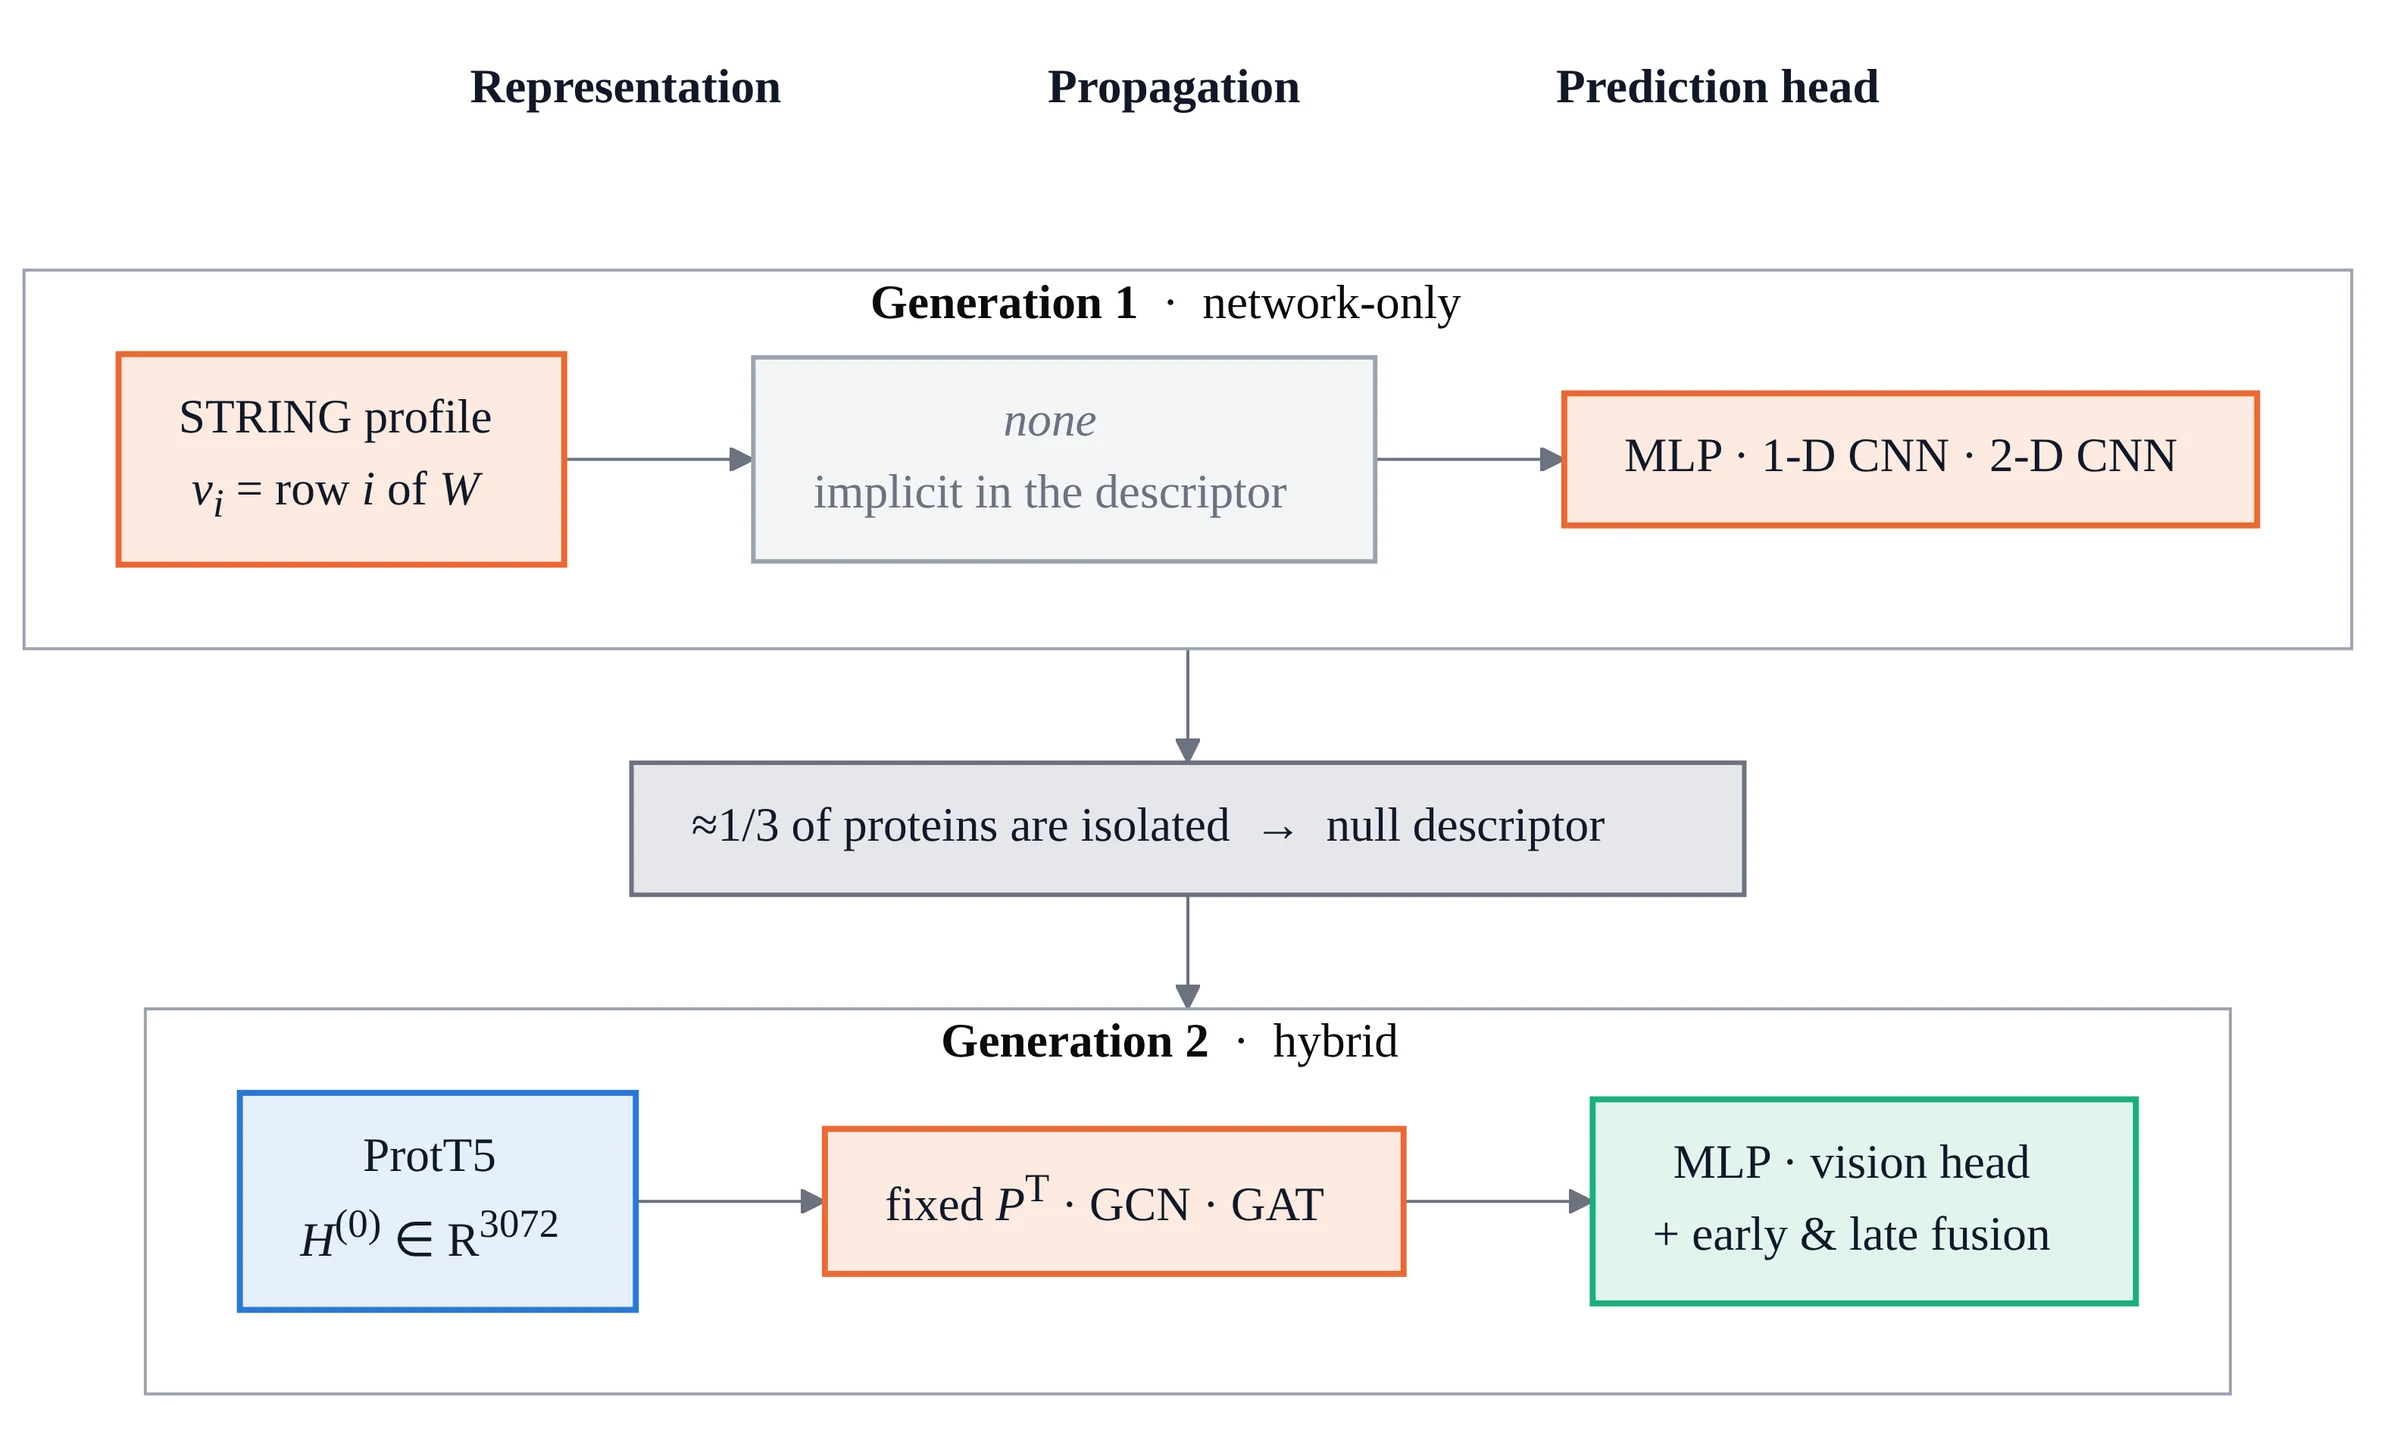
\includegraphics[width=896.7\px,height=535.4\px]{figures/fig_5_1.png}};
\fill<2>[plate] (109,315.3) rectangle ++(896.7,182);
\fill<2-3>[plate] (109,497.3) rectangle ++(896.7,91);
\fill<2-4>[plate] (109,588.3) rectangle ++(896.7,182);
\node[tl] at (88,70) {\fmR\fz{16}{16}\color{inkii}\ls{2}\Ll{4 · Method}};
\node[tl] at (88,131) {\fdA\fz{54}{56.7}\color{ink}\ls{-1}\Ll{Two generations, three decisions}};
\node<2-5>[tl] at (88,808.4) {\fmR\fz{15}{19.5}\color{muted}\Ll{Dissertation, Fig. 5.1}};
\node<2-5>[tl] at (1094.7,236) {\fbR\fz{30}{40.5}\color{ink}\Ll{Representation $\rightarrow$ Propagation\\$\rightarrow$ Prediction head}};
\node<3-5>[tl] at (1094.7,339) {\fbR\fz{30}{40.5}\color{ink}\Ll{Generation 1: network only}};
\node<5>[tl] at (1094.7,401.5) {\fbR\fz{30}{40.5}\color{ink}\Ll{Generation 2 (NEXUS-GO):\\ProtT5 + network}};
\node[tr] at (1512,876) {\fmR\fz{16}{16}\color{muted}18 / 45};
\end{tikzpicture}
\note{Every model decomposes into the same three decisions: representation, propagation and prediction head. 

The limitation of the first generation is a property of its input, about one third of the proteins get a null descriptor, and it motivates the second.}
\end{frame}

\begin{frame}[plain]
\begin{tikzpicture}[deck]
\node<1>[box] at (0,0) {\includegraphics[page=3,width=1600\px]{build/layers}};
\node<2>[box] at (0,0) {\includegraphics[page=53,width=1600\px]{build/layers}};
\node<3>[box] at (0,0) {\includegraphics[page=54,width=1600\px]{build/layers}};
\node<4>[box] at (0,0) {\includegraphics[page=55,width=1600\px]{build/layers}};
\node<2-4>[box] at (109,235) {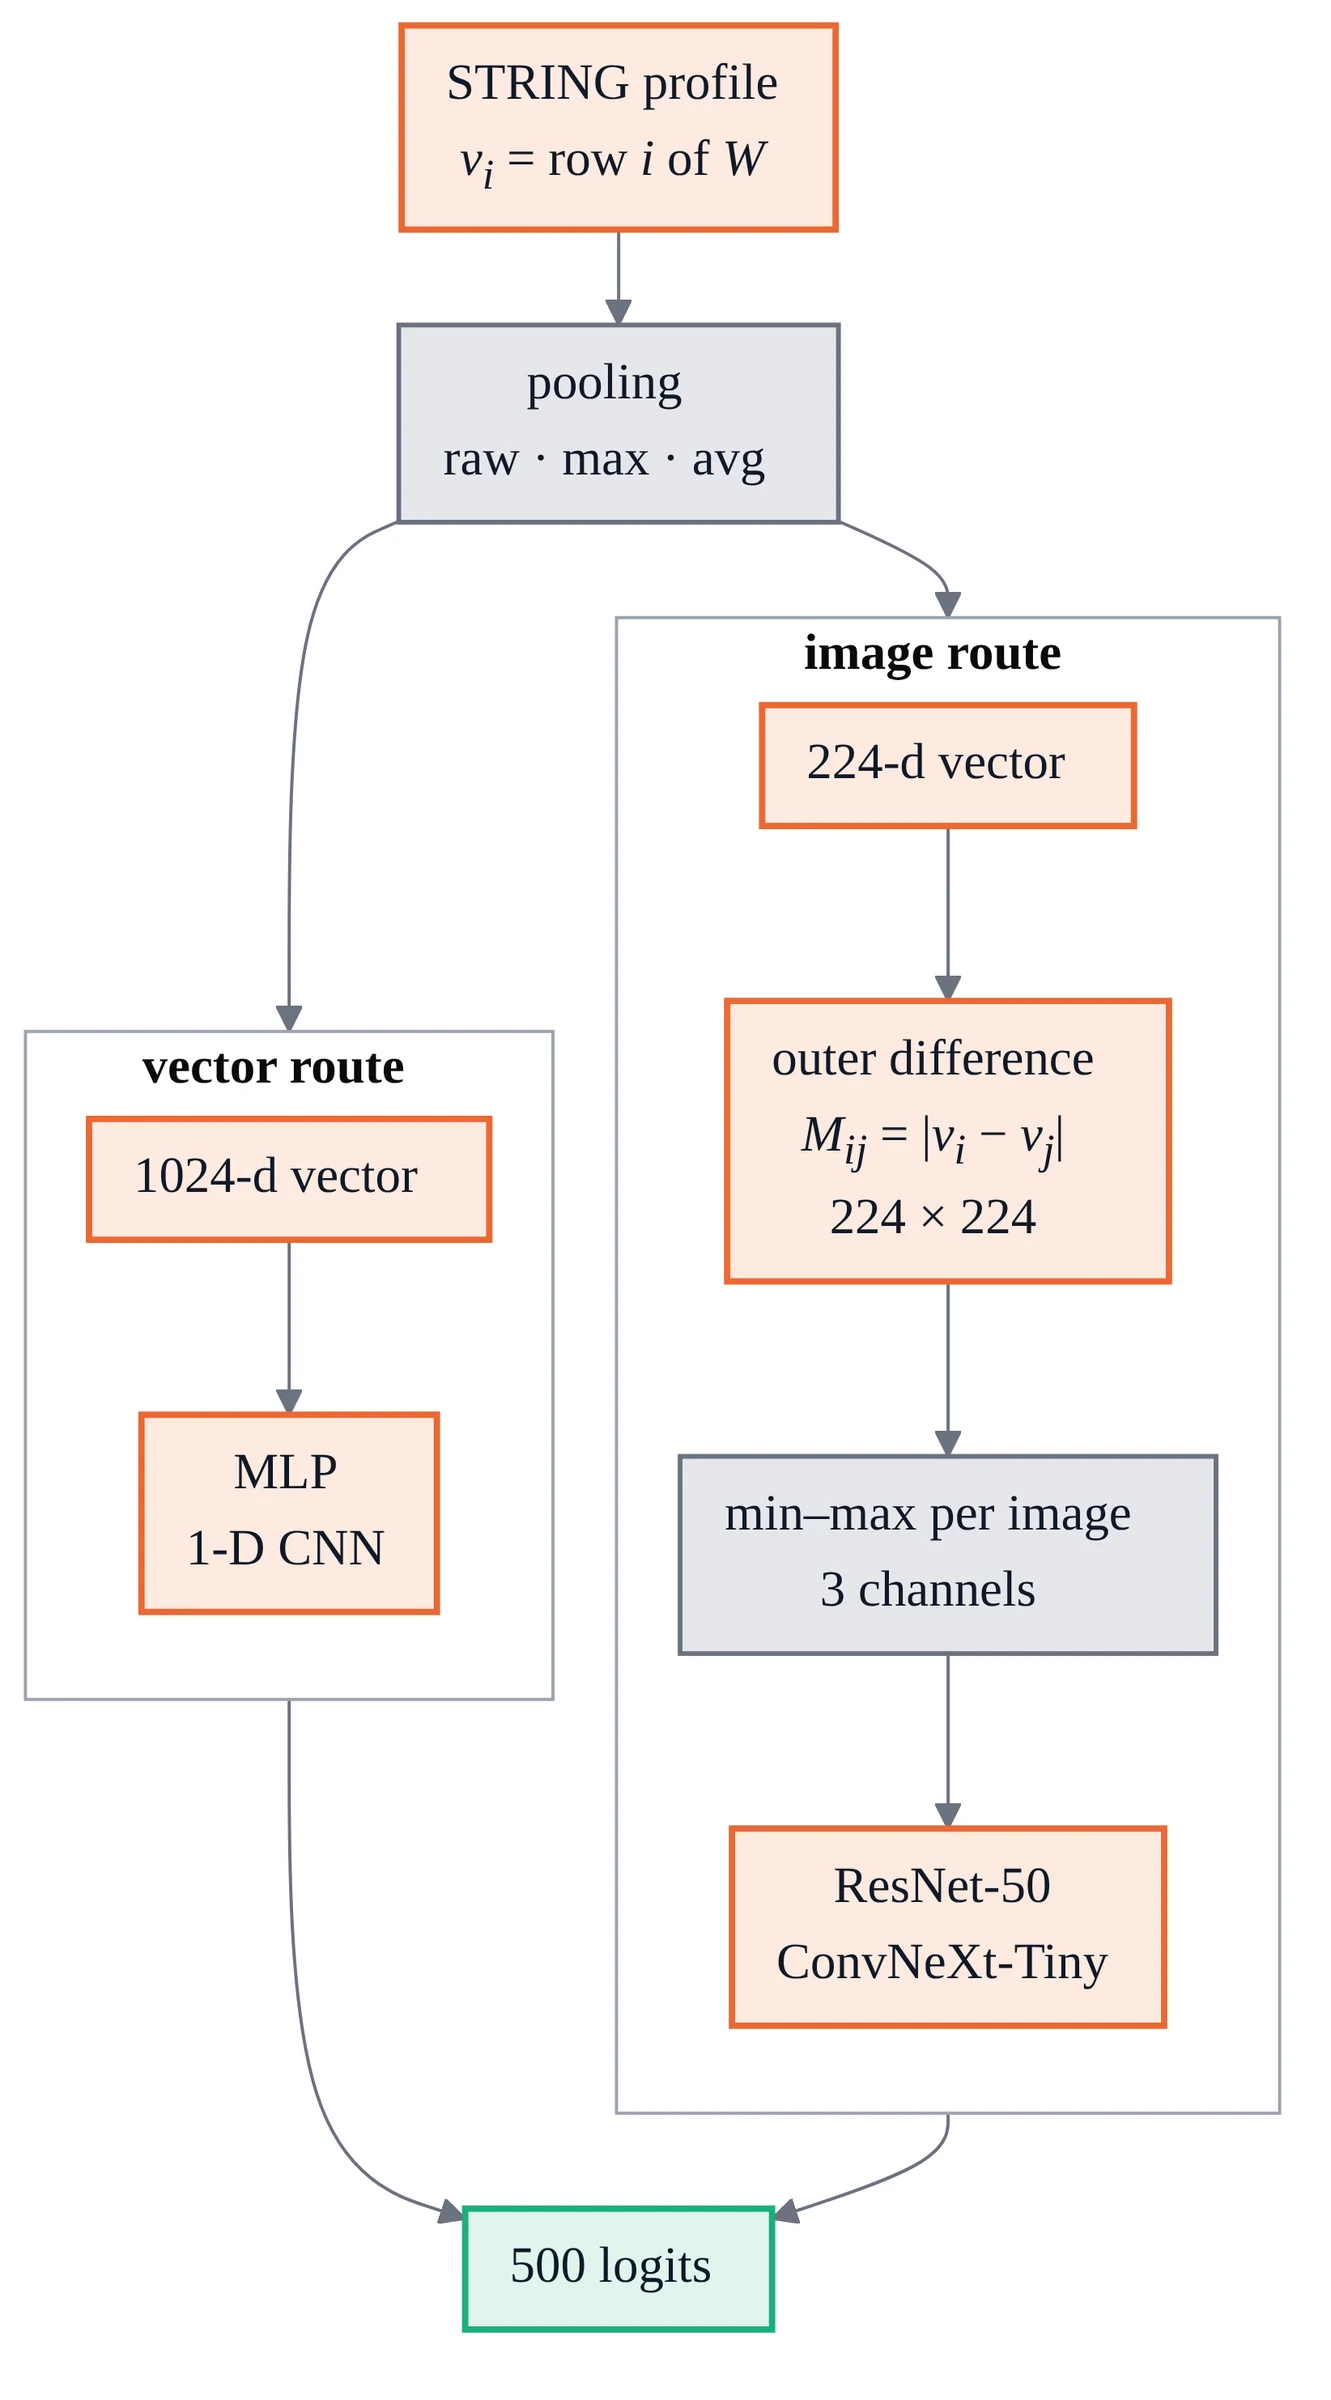
\includegraphics[width=299.5\px,height=540\px]{figures/fig_5_3.png}};
\node<4>[box] at (473,512.5) {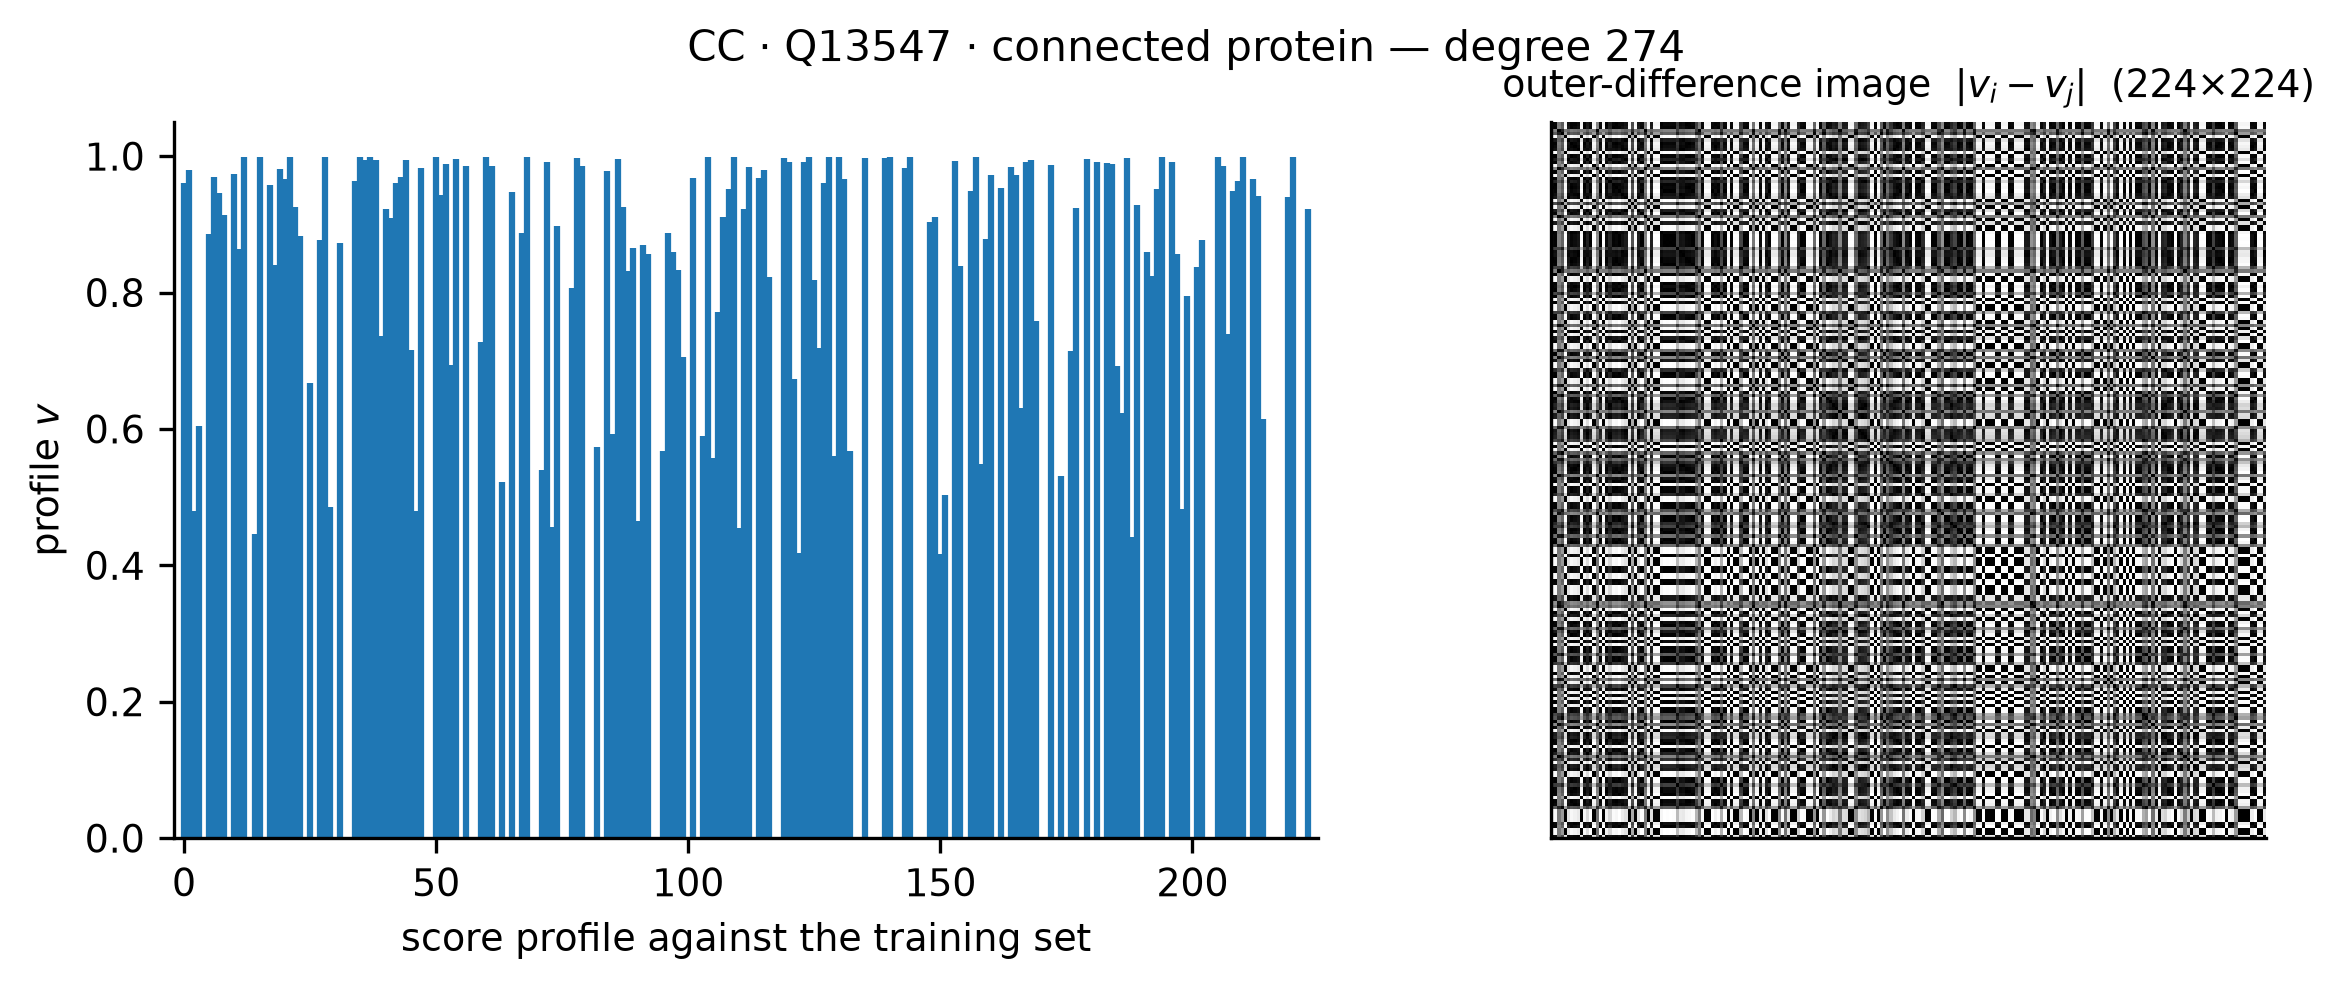
\includegraphics[width=592.2\px,height=250\px]{figures/fig_5_4.png}};
\node[tl] at (88,70) {\fmR\fz{16}{16}\color{inkii}\ls{2}\Ll{4 · Method}};
\node[tl] at (88,131) {\fdA\fz{54}{56.7}\color{ink}\ls{-1}\Ll{Generation 1: the network alone}};
\node<2-4>[tl] at (88,813) {\fmR\fz{15}{19.5}\color{muted}\Ll{Dissertation, Fig. 5.3}};
\node<2-4>[tl] at (488,232) {\fbR\fz{26}{35.1}\color{ink}\Ll{Input: row of the weighted adjacency, against training proteins}};
\node<2-4>[tl] at (488,283.1) {\fbR\fz{26}{35.1}\color{ink}\Ll{Pooling: raw, max, avg}};
\node<3-4>[tl] at (488,334.2) {\fbR\fz{26}{35.1}\color{ink}\Ll{Vector route: MLP or 1-D CNN}};
\node<4>[tl] at (488,385.3) {\fbR\fz{26}{35.1}\color{ink}\Ll{Image route: outer-difference matrix {\fz{29.2}{35}$|v_i - v_j|$}, 224 × 224, ResNet-50 or ConvNeXt-Tiny}};
\node<4>[tl] at (488,436.4) {\fbR\fz{26}{35.1}\color{ink}\Ll{Floor: a naive guilt-by-association baseline}};
\node<4>[tl] at (452,800.5) {\fmR\fz{15}{19.5}\color{muted}\Ll{Dissertation, Fig. 5.4}};
\node[tr] at (1512,876) {\fmR\fz{16}{16}\color{muted}19 / 45};
\end{tikzpicture}
\note{The descriptor is already a one-hop aggregation, so there is no separate propagation stage. 

The image route imports a convolutional bias into a non-visual vector, as SUPERMAGOv2 and DeepInsight did with isolated descriptors.}
\end{frame}

\begin{frame}[plain]
\begin{tikzpicture}[deck]
\node<1>[box] at (0,0) {\includegraphics[page=3,width=1600\px]{build/layers}};
\node<2>[box] at (0,0) {\includegraphics[page=56,width=1600\px]{build/layers}};
\node<3>[box] at (0,0) {\includegraphics[page=57,width=1600\px]{build/layers}};
\node<4>[box] at (0,0) {\includegraphics[page=58,width=1600\px]{build/layers}};
\node<2-4>[box] at (109,235) {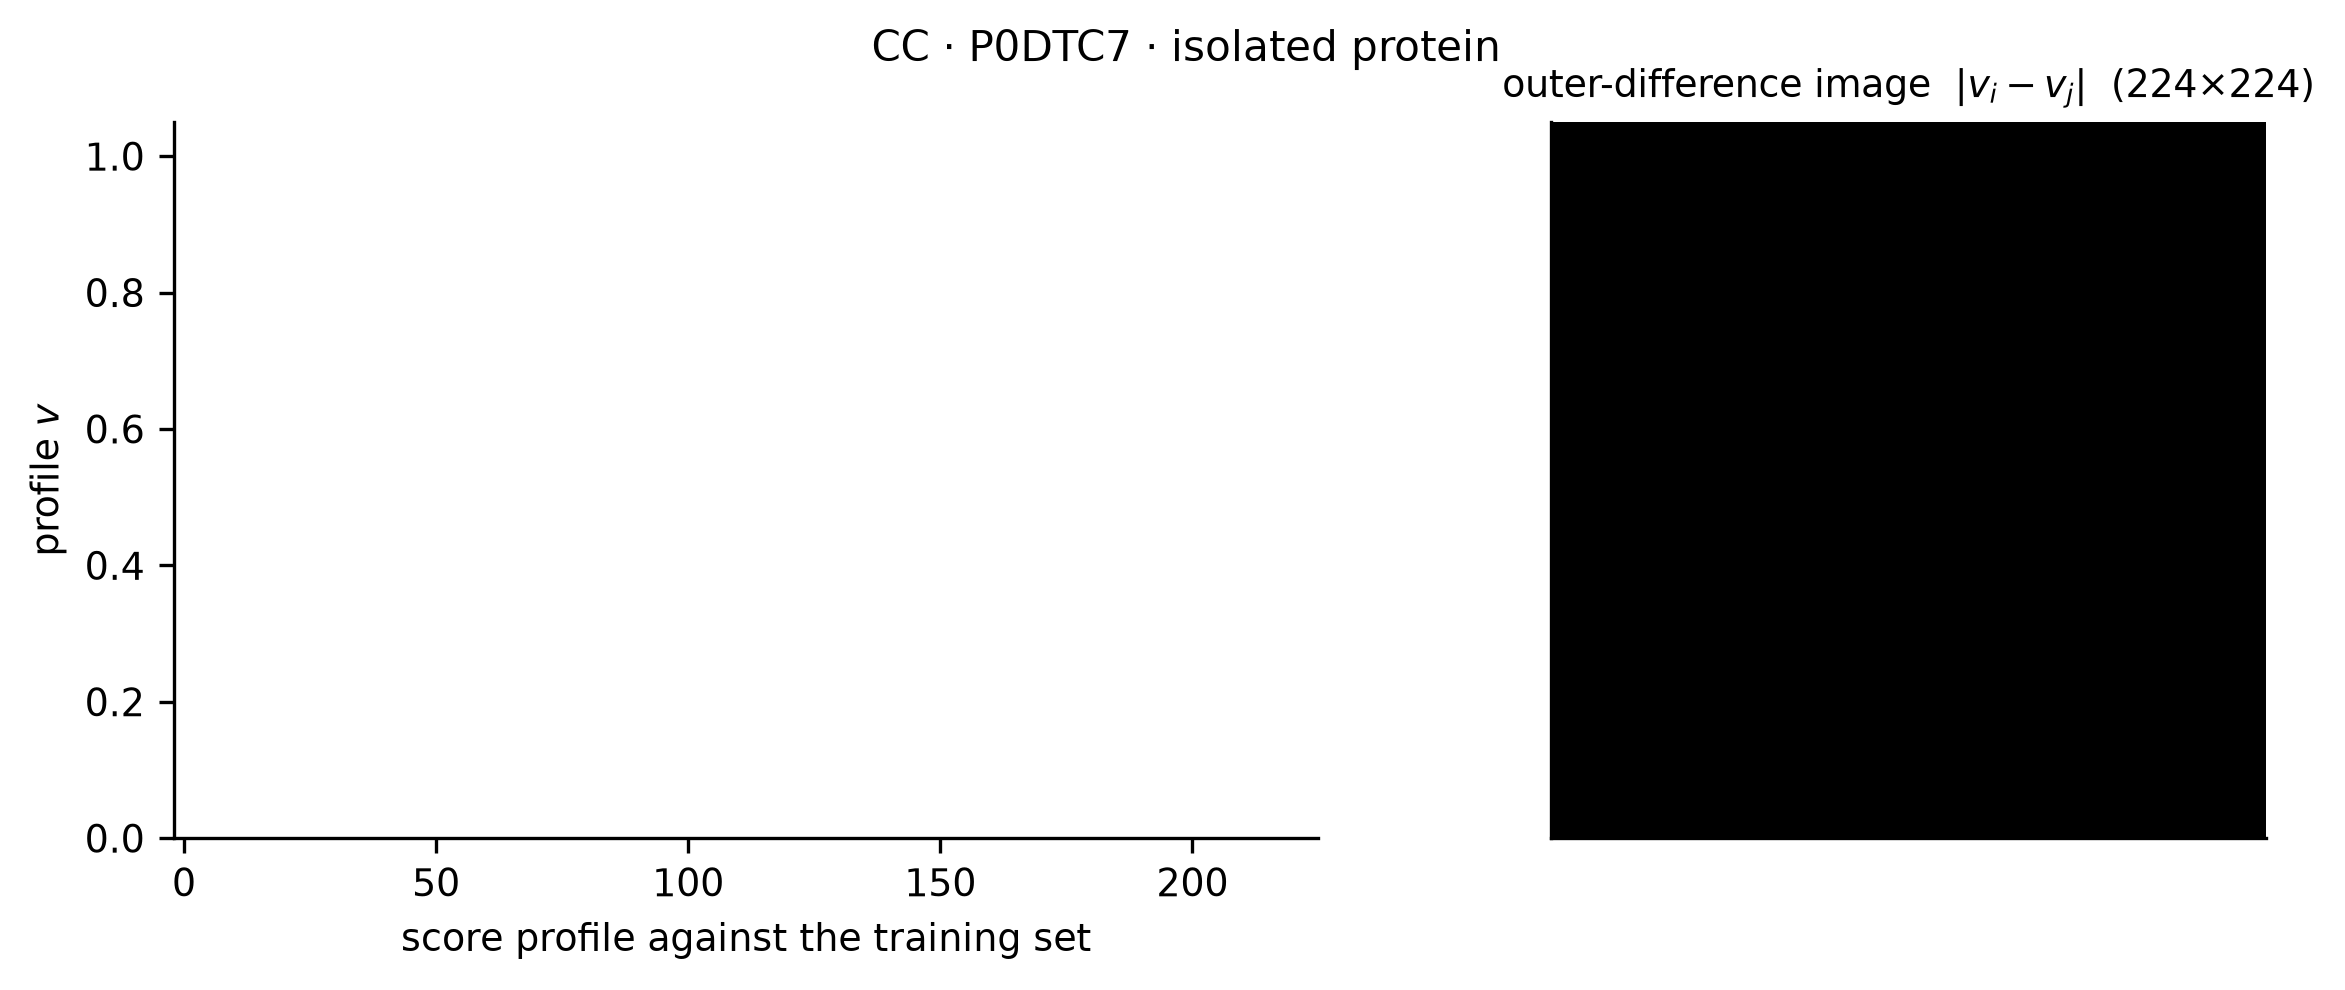
\includegraphics[width=654\px,height=276.1\px]{figures/fig_5_5.png}};
\node<2-4>[box] at (837,235) {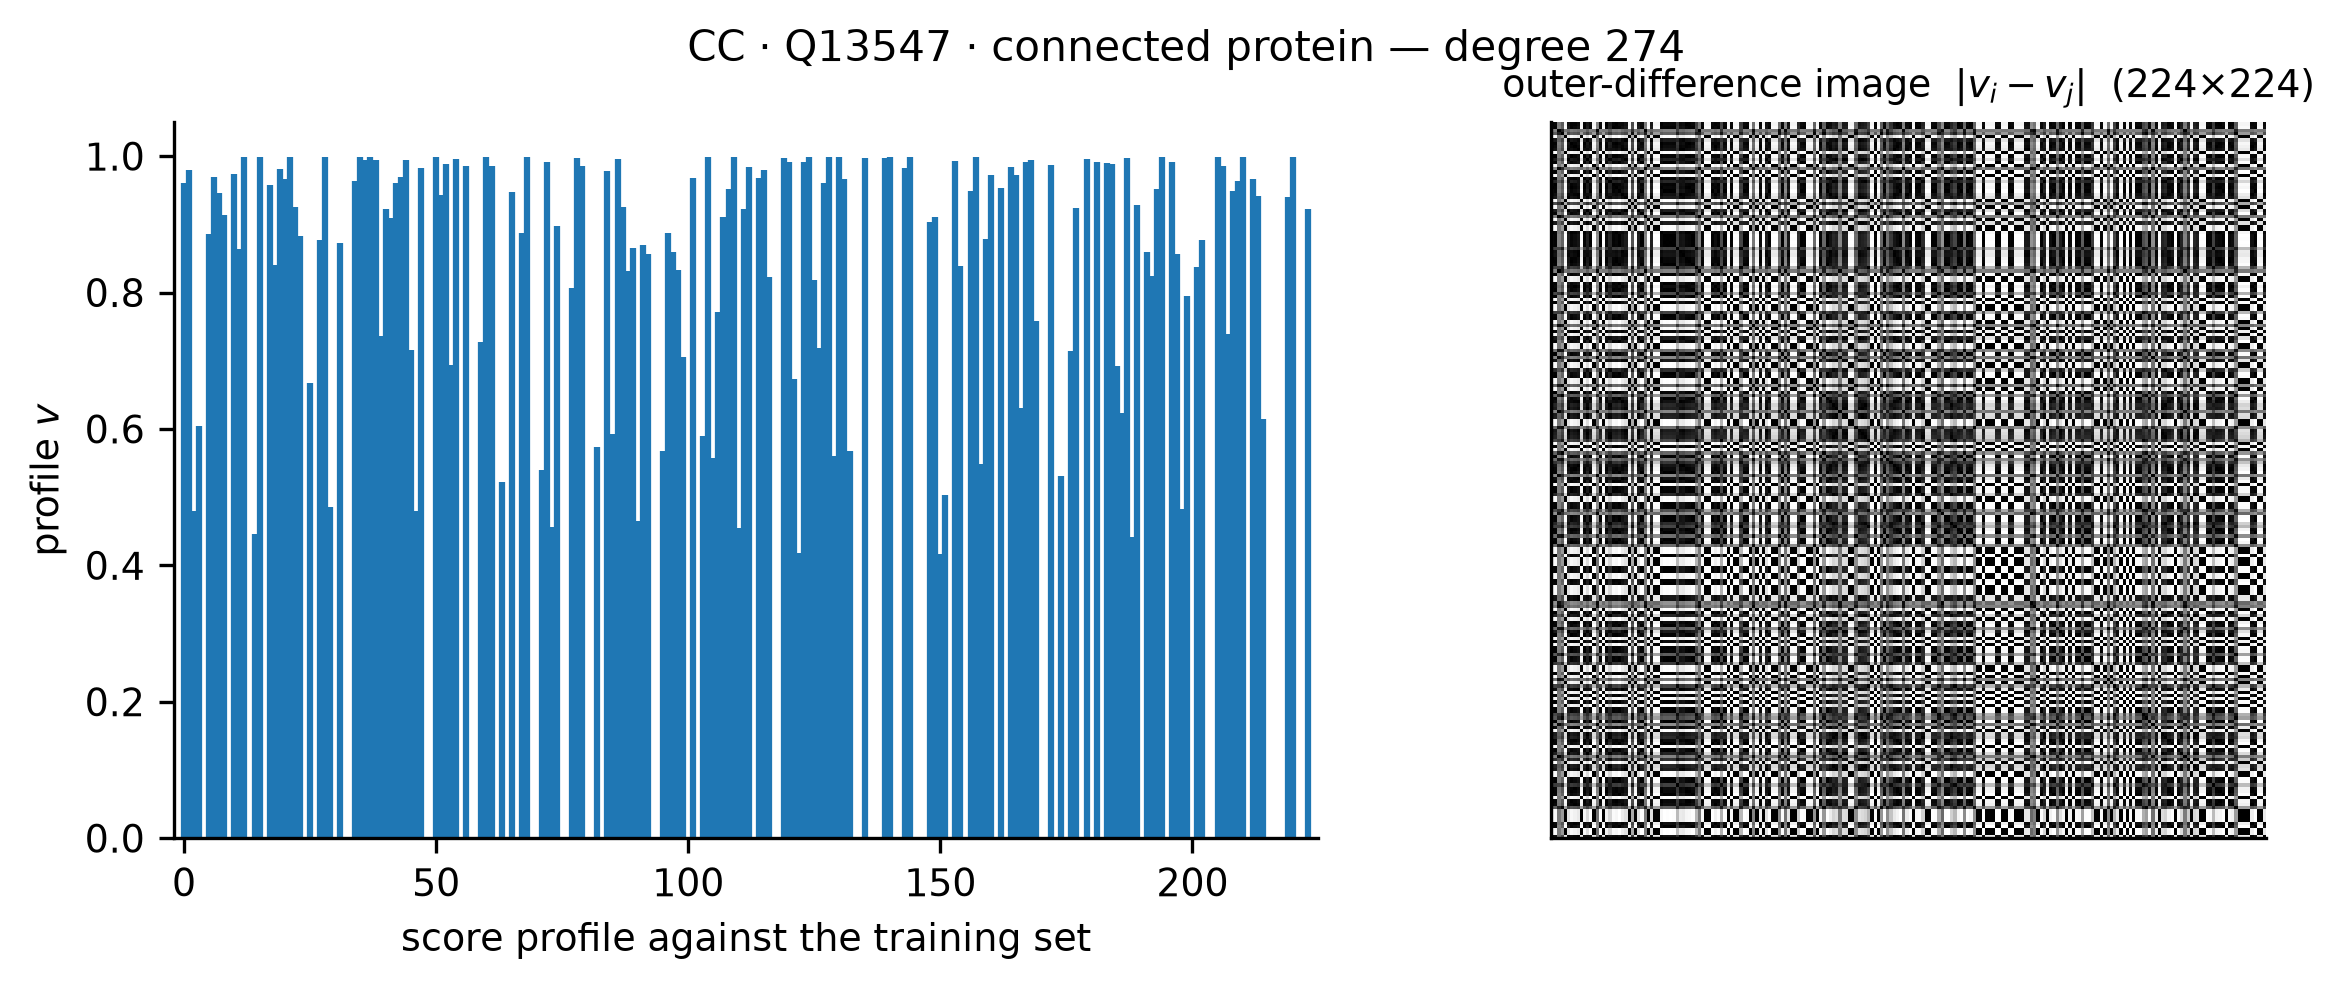
\includegraphics[width=654\px,height=276.1\px]{figures/fig_5_4.png}};
\node[tl] at (88,70) {\fmR\fz{16}{16}\color{inkii}\ls{2}\Ll{4 · Method}};
\node[tl] at (88,131) {\fdA\fz{54}{56.7}\color{ink}\ls{-1}\Ll{An isolated protein has no input}};
\node<2-4>[tl] at (88,549.1) {\fmR\fz{15}{19.5}\color{muted}\Ll{Dissertation, Fig. 5.5 · isolated vs connected}};
\node<2-4>[tl] at (816,549.1) {\fmR\fz{15}{19.5}\color{muted}\Ll{Dissertation, Fig. 5.4 · for contrast}};
\node<3-4>[tl] at (124,583.3) {\fbR\fz{30}{40.5}\color{ink}\Ll{Null profile $\rightarrow$ null matrix $\rightarrow$ uniform image}};
\node<3-4>[tl] at (124,645.8) {\fbR\fz{30}{40.5}\color{ink}\Ll{The head can only return the class prior}};
\node<3-4>[tl] at (124,708.3) {\fbR\fz{30}{40.5}\color{ink}\Ll{No architecture can recover what is absent}};
\node<4>[tl] at (846,779.8) {\fdA\fz{38}{45.6}\color{ink}\Ll{Requirement: a representation\\that exists for every protein}};
\node[tr] at (1512,876) {\fmR\fz{16}{16}\color{muted}20 / 45};
\end{tikzpicture}
\note{For a third of the corpus the first generation sees nothing. 

The amino-acid sequence satisfies the requirement by construction, and that is where the second generation starts.}
\end{frame}

\begin{frame}[plain]
\hypertarget<1>{s21.1}{}
\hypertarget<2>{s21.2}{}
\hypertarget<3>{s21.3}{}
\hypertarget<4>{s21.4}{}
\hypertarget<5>{s21.5}{}
\hypertarget<6>{s21.6}{}
\hypertarget<7>{s21.7}{}
\hypertarget<8>{s21.8}{}
\begin{tikzpicture}[deck]
\node<1>[box] at (0,0) {\includegraphics[page=59,width=1600\px]{build/layers}};
\node<2>[box] at (0,0) {\includegraphics[page=60,width=1600\px]{build/layers}};
\node<3>[box] at (0,0) {\includegraphics[page=61,width=1600\px]{build/layers}};
\node<4>[box] at (0,0) {\includegraphics[page=62,width=1600\px]{build/layers}};
\node<5>[box] at (0,0) {\includegraphics[page=63,width=1600\px]{build/layers}};
\node<6>[box] at (0,0) {\includegraphics[page=64,width=1600\px]{build/layers}};
\node<7>[box] at (0,0) {\includegraphics[page=65,width=1600\px]{build/layers}};
\node<8>[box] at (0,0) {\includegraphics[page=66,width=1600\px]{build/layers}};
\node<4-8>[box] at (207.4,206) {\hot{89.1}{42}{s21.4}};
\node<4-8>[box] at (295,206) {\hot{82.5}{42}{s21.5}};
\node<4-8>[box] at (376,206) {\hot{84.8}{42}{s21.6}};
\node<4-8>[box] at (459.4,206) {\hot{80}{42}{s21.7}};
\node<4-8>[box] at (152,206) {\hot{56.9}{42}{s21.8}};
\node<4-8>[box] at (1315.5,206) {\hot{196.5}{42}{s21fig}};
\fill<8>[slide] (86,204) rectangle ++(1428,544); \node<8>[box] at (88,206) {\animategraphics[autoplay,loop,width=1424\px]{10}{build/seq/pipe-anim}{}{}};
\node[tl] at (88,70) {\fmR\fz{16}{16}\color{inkii}\ls{2}\Ll{4 · Method}};
\node[tl] at (88,131) {\fdA\fz{54}{56.7}\color{ink}\ls{-1}\Ll{NEXUS-GO: four routes}};
\node<2-8>[tl] at (88,803.1) {\fbR\fz{24}{31.2}\color{ink}\Ll{Sequence $\rightarrow$ ProtT5 $\rightarrow$ {\fz{26.9}{32.3}$\mathbf{H}^{(0)} \in \mathbb{R}^{3072}$}}};
\node<3-8>[tl] at (573.3,802) {\fbR\fz{24}{31.2}\color{ink}\Ll{STRING $\rightarrow$ weighted graph {\fz{26.9}{32.3}$W$} $\rightarrow$\\{\fz{26.9}{32.3}$P = W D_c^{-1}$}}};
\node<4-8>[tl] at (1058.7,802) {\fbR\fz{24}{31.2}\color{ink}\Ll{Routes: /Fixed · /GNN · /Early · /Late}};
\node[tr] at (1512,876) {\fmR\fz{16}{16}\color{muted}21 / 45};
\end{tikzpicture}
\note{Two inputs, two propagation routes and two ways of combining them. 

The first generation is reported as a topology-only control and carries no route name.}
\end{frame}

\begin{frame}[plain]
\begin{tikzpicture}[deck]
\node<1>[box] at (0,0) {\includegraphics[page=3,width=1600\px]{build/layers}};
\node<2>[box] at (0,0) {\includegraphics[page=67,width=1600\px]{build/layers}};
\node<3>[box] at (0,0) {\includegraphics[page=68,width=1600\px]{build/layers}};
\node<4>[box] at (0,0) {\includegraphics[page=69,width=1600\px]{build/layers}};
\node<2-4>[box] at (109,235) {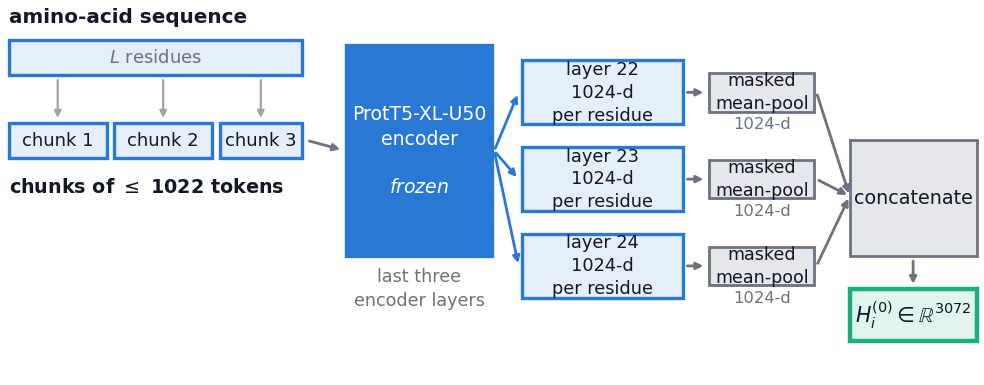
\includegraphics[width=1022.3\px,height=400\px]{figures/fig_5_7.png}};
\node[tl] at (88,70) {\fmR\fz{16}{16}\color{inkii}\ls{2}\Ll{4 · Method}};
\node[tl] at (88,131) {\fdA\fz{54}{56.7}\color{ink}\ls{-1}\Ll{ProtT5-XL-U50, three layers, frozen}};
\node<2-4>[tl] at (88,673) {\fmR\fz{15}{19.5}\color{muted}\Ll{Dissertation, Fig. 5.7}};
\node<2-4>[tl] at (124,729.5) {\fbR\fz{26}{35.1}\color{ink}\Ll{Chunks of at most 1,022 residues;\\masked mean-pool, then mean\\over chunks}};
\node<3-4>[tl] at (609.3,729.5) {\fbR\fz{26}{35.1}\color{ink}\Ll{Layers 24, 23, 22, concatenated: 3 ×\\1024 = 3072 dimensions}};
\node<4>[tl] at (1094.7,729.5) {\fbR\fz{26}{35.1}\color{ink}\Ll{Exists for every protein, isolated\\or not}};
\node[tr] at (1512,876) {\fmR\fz{16}{16}\color{muted}22 / 45};
\end{tikzpicture}
\note{Reading three adjacent layers avoids committing to one point between the pretraining objective and structural signal, at no tuning cost. 

Extraction is inherited from SUPERMAGOv2.}
\end{frame}

\begin{frame}[plain]
\hypertarget<1>{s23.1}{}
\hypertarget<2>{s23.2}{}
\hypertarget<3>{s23.3}{}
\hypertarget<4>{s23.4}{}
\hypertarget<5>{s23.5}{}
\begin{tikzpicture}[deck]
\node<1>[box] at (0,0) {\includegraphics[page=3,width=1600\px]{build/layers}};
\node<2>[box] at (0,0) {\includegraphics[page=70,width=1600\px]{build/layers}};
\node<3>[box] at (0,0) {\includegraphics[page=71,width=1600\px]{build/layers}};
\node<4>[box] at (0,0) {\includegraphics[page=72,width=1600\px]{build/layers}};
\node<5>[box] at (0,0) {\includegraphics[page=73,width=1600\px]{build/layers}};
\node<3-5>[box] at (749.1,206) {\hot{71.1}{42}{s23.4}};
\node<3-5>[box] at (818.7,206) {\hot{71}{42}{s23.5}};
\node[tl] at (88,70) {\fmR\fz{16}{16}\color{inkii}\ls{2}\Ll{4 · Method}};
\node[tl] at (88,131) {\fdA\fz{54}{56.7}\color{ink}\ls{-1}\Ll{From records to an operator}};
\node<2-5>[tl] at (124,236) {\fbR\fz{30}{40.5}\color{ink}\Ll{Symmetric, no self-loops, sparse COO: at\\most 1,133,132 stored entries (dense: 25\\to 35 GB)}};
\node<3-5>[tl] at (124,379.5) {\fbR\fz{30}{40.5}\color{ink}\Ll{Deduplication: max keeps the score;\\sum multiplies it by the record count}};
\node<4-5>[tl] at (124,482.5) {\fbR\fz{30}{40.5}\color{ink}\Ll{Column-stochastic {\fz{33.7}{40.4}$P = W D_c^{-1}$}: weights\\are relative to each protein's neighbours}};
\node[tr] at (1512,876) {\fmR\fz{16}{16}\color{muted}23 / 45};
\end{tikzpicture}
\note{Repeated records carry no extra score, so summing rewards how often a pair was written down. The maximum keeps the STRING score on its own scale. 

Normalization does not undo the reordering.}
\end{frame}

\begin{frame}[plain]
\hypertarget<1>{s24.1}{}
\hypertarget<2>{s24.2}{}
\hypertarget<3>{s24.3}{}
\hypertarget<4>{s24.4}{}
\hypertarget<5>{s24.5}{}
\hypertarget<6>{s24.6}{}
\hypertarget<7>{s24.7}{}
\hypertarget<8>{s24.8}{}
\begin{tikzpicture}[deck]
\node<1-2>[box] at (0,0) {\includegraphics[page=3,width=1600\px]{build/layers}};
\node<3>[box] at (0,0) {\includegraphics[page=74,width=1600\px]{build/layers}};
\node<4>[box] at (0,0) {\includegraphics[page=75,width=1600\px]{build/layers}};
\node<5,8>[box] at (0,0) {\includegraphics[page=76,width=1600\px]{build/layers}};
\node<6>[box] at (0,0) {\includegraphics[page=77,width=1600\px]{build/layers}};
\node<7>[box] at (0,0) {\includegraphics[page=78,width=1600\px]{build/layers}};
\node<3>[box] at (800.2,211) {\hot{13.6}{32}{s24.6}};
\node<3>[box] at (813.9,211) {\hot{11.2}{32}{s24x.46}};
\node<3>[box] at (825,211) {\hot{11.2}{32}{s24.5}};
\node<3>[box] at (836.2,211) {\hot{11.2}{32}{s24x.48}};
\node<3>[box] at (847.5,211) {\hot{11.2}{32}{s24x.49}};
\node<3>[box] at (858.6,211) {\hot{11.2}{32}{s24x.50}};
\node<3>[box] at (869.9,211) {\hot{11.2}{32}{s24.7}};
\node<3>[box] at (881,211) {\hot{11.2}{32}{s24x.52}};
\node<3>[box] at (892.2,211) {\hot{11.2}{32}{s24x.53}};
\node<3>[box] at (903.5,211) {\hot{11.2}{32}{s24x.54}};
\node<3>[box] at (914.6,211) {\hot{13.6}{32}{s24x.55}};
\node<3>[box] at (1139.7,211) {\hot{15}{32}{s24x.3}};
\node<3>[box] at (1154.7,211) {\hot{14}{32}{s24x.14}};
\node<3>[box] at (1168.7,211) {\hot{14}{32}{s24x.25}};
\node<3>[box] at (1182.7,211) {\hot{14}{32}{s24x.36}};
\node<3>[box] at (1196.7,211) {\hot{14}{32}{s24.5}};
\node<3>[box] at (1210.7,211) {\hot{14}{32}{s24x.58}};
\node<3>[box] at (1224.7,211) {\hot{14}{32}{s24x.69}};
\node<3>[box] at (1238.7,211) {\hot{14}{32}{s24x.80}};
\node<3>[box] at (1252.7,211) {\hot{15}{32}{s24x.91}};
\node<3>[box] at (1337.3,206) {\hot{70.2}{42}{s24.8}};
\node<4>[box] at (800.2,211) {\hot{13.6}{32}{s24.6}};
\node<4>[box] at (813.9,211) {\hot{11.2}{32}{s24x.46}};
\node<4>[box] at (825,211) {\hot{11.2}{32}{s24.5}};
\node<4>[box] at (836.2,211) {\hot{11.2}{32}{s24x.48}};
\node<4>[box] at (847.5,211) {\hot{11.2}{32}{s24x.49}};
\node<4>[box] at (858.6,211) {\hot{11.2}{32}{s24x.50}};
\node<4>[box] at (869.9,211) {\hot{11.2}{32}{s24.7}};
\node<4>[box] at (881,211) {\hot{11.2}{32}{s24x.52}};
\node<4>[box] at (892.2,211) {\hot{11.2}{32}{s24x.53}};
\node<4>[box] at (903.5,211) {\hot{11.2}{32}{s24x.54}};
\node<4>[box] at (914.6,211) {\hot{13.6}{32}{s24x.55}};
\node<4>[box] at (1139.7,211) {\hot{15}{32}{s24x.3}};
\node<4>[box] at (1154.7,211) {\hot{14}{32}{s24x.14}};
\node<4>[box] at (1168.7,211) {\hot{14}{32}{s24x.25}};
\node<4>[box] at (1182.7,211) {\hot{14}{32}{s24x.36}};
\node<4>[box] at (1196.7,211) {\hot{14}{32}{s24.5}};
\node<4>[box] at (1210.7,211) {\hot{14}{32}{s24x.58}};
\node<4>[box] at (1224.7,211) {\hot{14}{32}{s24x.69}};
\node<4>[box] at (1238.7,211) {\hot{14}{32}{s24x.80}};
\node<4>[box] at (1252.7,211) {\hot{15}{32}{s24x.91}};
\node<4>[box] at (1337.3,206) {\hot{70.2}{42}{s24.8}};
\node<5>[box] at (800.2,211) {\hot{13.6}{32}{s24.6}};
\node<5>[box] at (813.9,211) {\hot{11.2}{32}{s24x.46}};
\node<5>[box] at (825,211) {\hot{11.2}{32}{s24.5}};
\node<5>[box] at (836.2,211) {\hot{11.2}{32}{s24x.48}};
\node<5>[box] at (847.5,211) {\hot{11.2}{32}{s24x.49}};
\node<5>[box] at (858.6,211) {\hot{11.2}{32}{s24x.50}};
\node<5>[box] at (869.9,211) {\hot{11.2}{32}{s24.7}};
\node<5>[box] at (881,211) {\hot{11.2}{32}{s24x.52}};
\node<5>[box] at (892.2,211) {\hot{11.2}{32}{s24x.53}};
\node<5>[box] at (903.5,211) {\hot{11.2}{32}{s24x.54}};
\node<5>[box] at (914.6,211) {\hot{13.6}{32}{s24x.55}};
\node<5>[box] at (1139.7,211) {\hot{15}{32}{s24x.3}};
\node<5>[box] at (1154.7,211) {\hot{14}{32}{s24x.14}};
\node<5>[box] at (1168.7,211) {\hot{14}{32}{s24x.25}};
\node<5>[box] at (1182.7,211) {\hot{14}{32}{s24x.36}};
\node<5>[box] at (1196.7,211) {\hot{14}{32}{s24.5}};
\node<5>[box] at (1210.7,211) {\hot{14}{32}{s24x.58}};
\node<5>[box] at (1224.7,211) {\hot{14}{32}{s24x.69}};
\node<5>[box] at (1238.7,211) {\hot{14}{32}{s24x.80}};
\node<5>[box] at (1252.7,211) {\hot{15}{32}{s24x.91}};
\node<5>[box] at (1337.3,206) {\hot{70.2}{42}{s24.8}};
\node<6>[box] at (800.2,211) {\hot{13.6}{32}{s24.6}};
\node<6>[box] at (813.9,211) {\hot{11.2}{32}{s24x.46}};
\node<6>[box] at (825,211) {\hot{11.2}{32}{s24.5}};
\node<6>[box] at (836.2,211) {\hot{11.2}{32}{s24x.48}};
\node<6>[box] at (847.5,211) {\hot{11.2}{32}{s24x.49}};
\node<6>[box] at (858.6,211) {\hot{11.2}{32}{s24x.50}};
\node<6>[box] at (869.9,211) {\hot{11.2}{32}{s24.7}};
\node<6>[box] at (881,211) {\hot{11.2}{32}{s24x.52}};
\node<6>[box] at (892.2,211) {\hot{11.2}{32}{s24x.53}};
\node<6>[box] at (903.5,211) {\hot{11.2}{32}{s24x.54}};
\node<6>[box] at (914.6,211) {\hot{13.6}{32}{s24x.55}};
\node<6>[box] at (1139.7,211) {\hot{15}{32}{s24x.1}};
\node<6>[box] at (1154.7,211) {\hot{14}{32}{s24x.12}};
\node<6>[box] at (1168.7,211) {\hot{14}{32}{s24x.23}};
\node<6>[box] at (1182.7,211) {\hot{14}{32}{s24x.34}};
\node<6>[box] at (1196.7,211) {\hot{14}{32}{s24.6}};
\node<6>[box] at (1210.7,211) {\hot{14}{32}{s24x.56}};
\node<6>[box] at (1224.7,211) {\hot{14}{32}{s24x.67}};
\node<6>[box] at (1238.7,211) {\hot{14}{32}{s24x.78}};
\node<6>[box] at (1252.7,211) {\hot{15}{32}{s24x.89}};
\node<6>[box] at (1337.3,206) {\hot{70.2}{42}{s24.8}};
\node<7>[box] at (800.2,211) {\hot{13.6}{32}{s24.6}};
\node<7>[box] at (813.9,211) {\hot{11.2}{32}{s24x.46}};
\node<7>[box] at (825,211) {\hot{11.2}{32}{s24.5}};
\node<7>[box] at (836.2,211) {\hot{11.2}{32}{s24x.48}};
\node<7>[box] at (847.5,211) {\hot{11.2}{32}{s24x.49}};
\node<7>[box] at (858.6,211) {\hot{11.2}{32}{s24x.50}};
\node<7>[box] at (869.9,211) {\hot{11.2}{32}{s24.7}};
\node<7>[box] at (881,211) {\hot{11.2}{32}{s24x.52}};
\node<7>[box] at (892.2,211) {\hot{11.2}{32}{s24x.53}};
\node<7>[box] at (903.5,211) {\hot{11.2}{32}{s24x.54}};
\node<7>[box] at (914.6,211) {\hot{13.6}{32}{s24x.55}};
\node<7>[box] at (1139.7,211) {\hot{15}{32}{s24x.7}};
\node<7>[box] at (1154.7,211) {\hot{14}{32}{s24x.18}};
\node<7>[box] at (1168.7,211) {\hot{14}{32}{s24x.29}};
\node<7>[box] at (1182.7,211) {\hot{14}{32}{s24x.40}};
\node<7>[box] at (1196.7,211) {\hot{14}{32}{s24.7}};
\node<7>[box] at (1210.7,211) {\hot{14}{32}{s24x.62}};
\node<7>[box] at (1224.7,211) {\hot{14}{32}{s24x.73}};
\node<7>[box] at (1238.7,211) {\hot{14}{32}{s24x.84}};
\node<7>[box] at (1252.7,211) {\hot{15}{32}{s24x.95}};
\node<7>[box] at (1337.3,206) {\hot{70.2}{42}{s24.8}};
\node<8>[box] at (800.2,211) {\hot{13.6}{32}{s24.6}};
\node<8>[box] at (813.9,211) {\hot{11.2}{32}{s24x.46}};
\node<8>[box] at (825,211) {\hot{11.2}{32}{s24.5}};
\node<8>[box] at (836.2,211) {\hot{11.2}{32}{s24x.48}};
\node<8>[box] at (847.5,211) {\hot{11.2}{32}{s24x.49}};
\node<8>[box] at (858.6,211) {\hot{11.2}{32}{s24x.50}};
\node<8>[box] at (869.9,211) {\hot{11.2}{32}{s24.7}};
\node<8>[box] at (881,211) {\hot{11.2}{32}{s24x.52}};
\node<8>[box] at (892.2,211) {\hot{11.2}{32}{s24x.53}};
\node<8>[box] at (903.5,211) {\hot{11.2}{32}{s24x.54}};
\node<8>[box] at (914.6,211) {\hot{13.6}{32}{s24x.55}};
\node<8>[box] at (1139.7,211) {\hot{15}{32}{s24x.3}};
\node<8>[box] at (1154.7,211) {\hot{14}{32}{s24x.14}};
\node<8>[box] at (1168.7,211) {\hot{14}{32}{s24x.25}};
\node<8>[box] at (1182.7,211) {\hot{14}{32}{s24x.36}};
\node<8>[box] at (1196.7,211) {\hot{14}{32}{s24.5}};
\node<8>[box] at (1210.7,211) {\hot{14}{32}{s24x.58}};
\node<8>[box] at (1224.7,211) {\hot{14}{32}{s24x.69}};
\node<8>[box] at (1238.7,211) {\hot{14}{32}{s24x.80}};
\node<8>[box] at (1252.7,211) {\hot{15}{32}{s24x.91}};
\node<8>[box] at (1337.3,206) {\hot{70.2}{42}{s24.8}};
\fill<8>[slide] (692.7,204) rectangle ++(821.3,634); \node<8>[box] at (694.7,206) {\animategraphics[autoplay,loop,width=817.3\px]{2}{build/seq/prop-anim}{}{}};
\node[tl] at (88,70) {\fmR\fz{16}{16}\color{inkii}\ls{2}\Ll{4 · Method}};
\node[tl] at (88,131) {\fdA\fz{54}{56.7}\color{ink}\ls{-1}\Ll{Fixed propagation: no parameters}};
\node<2-8>[tl] at (88,237.7) {\fbR\fz{30}{36}\color{ink}\Ll{{\fz{33.7}{40.4}$\displaystyle \mathbf{H}^{(h)} = \alpha\, \mathbf{H}^{(h-1)} + (1-\alpha)\, P^{\top} \mathbf{H}^{(h-1)}$}}};
\node<2-8>[tl] at (88,278.2) {\fbR\fz{24}{32.4}\color{inkii}\Ll{{\fz{26.9}{32.3}$h = 1, \dots, T$}}};
\node<4-8>[tl] at (124,346.6) {\fbR\fz{26}{35.1}\color{ink}\Ll{Closed form: hop {\fz{29.2}{35}$k$} gets weight\\[0.9\px]{\fz{29.2}{35}$\binom{T}{k}\, \alpha^{T-k} (1-\alpha)^{k}$}}};
\node<4-8>[tl] at (124,434.9) {\fbR\fz{26}{35.1}\color{ink}\Ll{Computed once, cached, reused every epoch}};
\node<5-8>[tl] at (124,486) {\fbR\fz{26}{35.1}\color{ink}\Ll{{\fz{29.2}{35}$T = 0$} or {\fz{29.2}{35}$\alpha = 1$}: the graph is switched off\\(internal control)}};
\node[tr] at (1512,876) {\fmR\fz{16}{16}\color{muted}24 / 45};
\end{tikzpicture}
\note{$\alpha$ retains part of the previous step, not of the original, so it slows mixing instead of re-injecting the input. 

The weights over hop counts are binomial with mean T(1 − $\alpha$). Unlike personalized PageRank, the initial state is never reintroduced.}
\end{frame}

\begin{frame}[plain]
\begin{tikzpicture}[deck]
\node<1>[box] at (0,0) {\includegraphics[page=3,width=1600\px]{build/layers}};
\node<2>[box] at (0,0) {\includegraphics[page=79,width=1600\px]{build/layers}};
\node<3>[box] at (0,0) {\includegraphics[page=80,width=1600\px]{build/layers}};
\node<4>[box] at (0,0) {\includegraphics[page=81,width=1600\px]{build/layers}};
\node<2-4>[box] at (109,235) {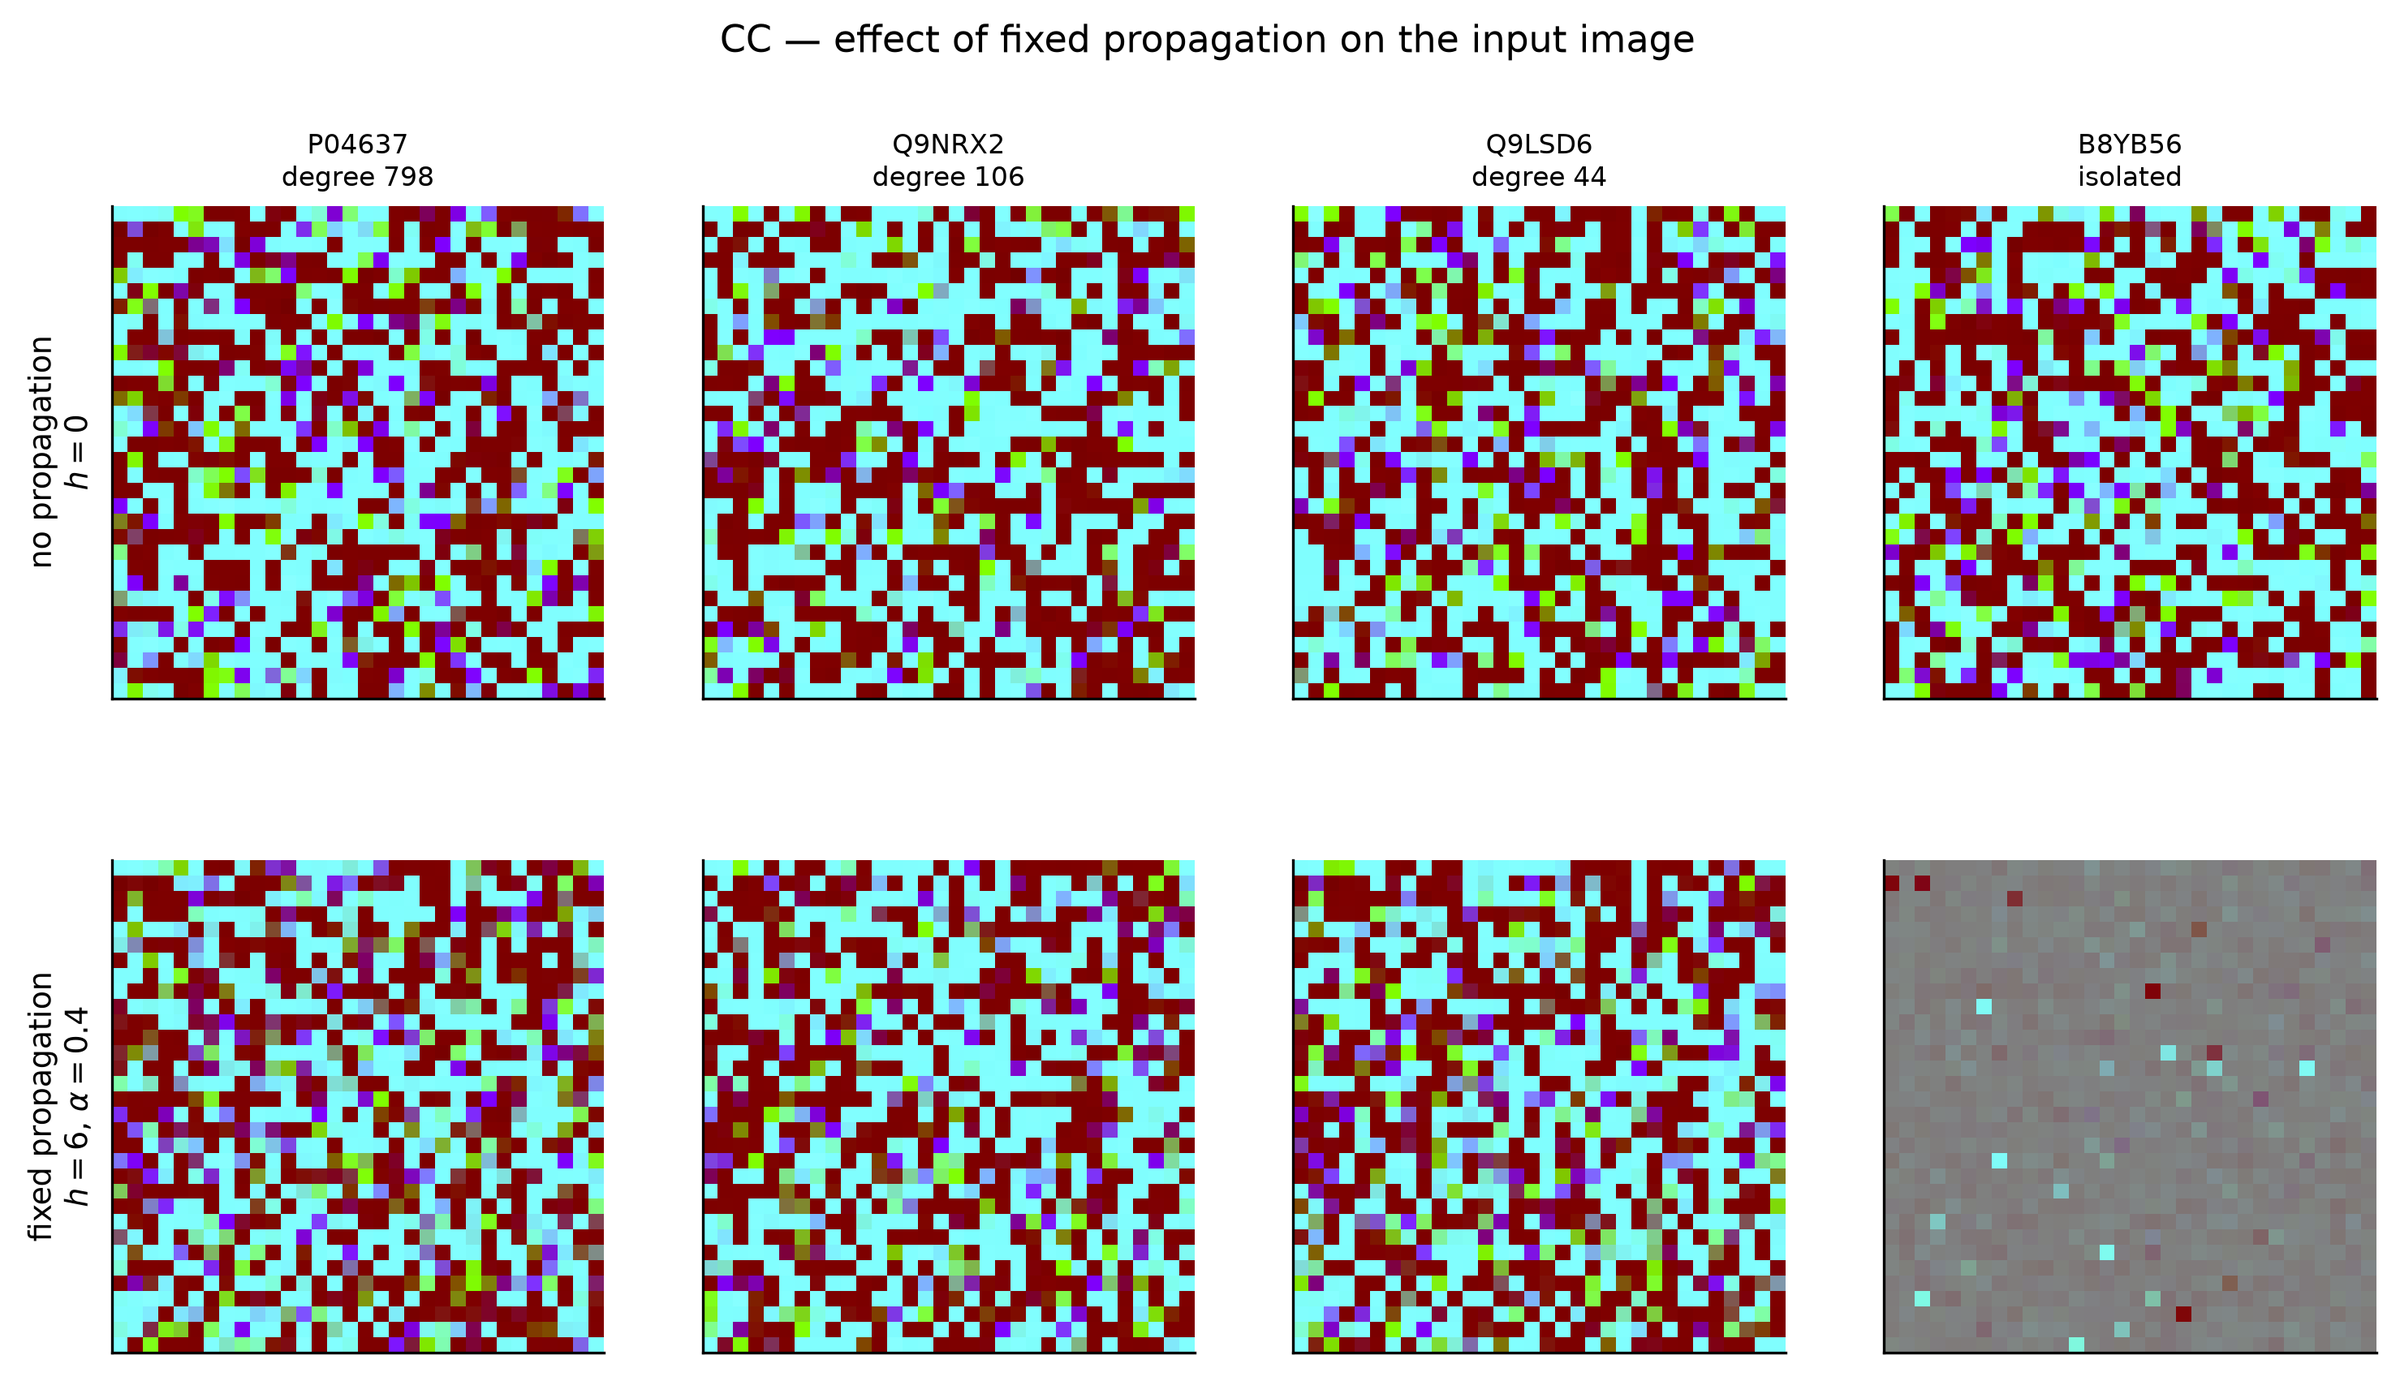
\includegraphics[width=896.7\px,height=514.5\px]{figures/fig_5_8.png}};
\node[tl] at (88,70) {\fmR\fz{16}{16}\color{inkii}\ls{2}\Ll{4 · Method}};
\node[tl] at (88,131) {\fdA\fz{54}{56.7}\color{ink}\ls{-1}\Ll{Propagation on four real proteins}};
\node<2-4>[tl] at (88,787.5) {\fmR\fz{15}{19.5}\color{muted}\Ll{Dissertation, Fig. 5.8 · CC, top {\fz{17.5}{21}$T = 0$}, bottom {\fz{17.5}{21}$T = 6,\ \alpha = 0.4$}}};
\node<3-4>[tl] at (1094.7,232) {\fbR\fz{26}{35.1}\color{ink}\Ll{Connected proteins keep their\\structure and absorb their\\neighbourhood}};
\node<4>[tl] at (1094.7,353.3) {\fbR\fz{26}{35.1}\color{ink}\Ll{An isolated protein becomes\\{\fz{29.2}{35}$\alpha^{T} \mathbf{H}^{(0)}$}: same direction,\\smaller scale}};
\node<4>[tl] at (1094.7,474.6) {\fbR\fz{26}{35.1}\color{ink}\Ll{So degree-zero gains cannot come\\from neighbourhood information}};
\node[tr] at (1512,876) {\fmR\fz{16}{16}\color{muted}25 / 45};
\end{tikzpicture}
\note{The rescaling is a structural property of the operator, not a tuned setting. 

The learned route adds self-loops and never mixes an isolated node with others.}
\end{frame}

\begin{frame}[plain]
\begin{tikzpicture}[deck]
\node<1>[box] at (0,0) {\includegraphics[page=3,width=1600\px]{build/layers}};
\node<2>[box] at (0,0) {\includegraphics[page=70,width=1600\px]{build/layers}};
\node<3>[box] at (0,0) {\includegraphics[page=82,width=1600\px]{build/layers}};
\node<4>[box] at (0,0) {\includegraphics[page=83,width=1600\px]{build/layers}};
\node<5>[box] at (0,0) {\includegraphics[page=84,width=1600\px]{build/layers}};
\node[tl] at (88,70) {\fmR\fz{16}{16}\color{inkii}\ls{2}\Ll{4 · Method}};
\node[tl] at (88,131) {\fdA\fz{54}{56.7}\color{ink}\ls{-1}\Ll{Learned propagation: GCN and GAT}};
\node<2-5>[tl] at (124,236) {\fbR\fz{30}{40.5}\color{ink}\Ll{GCN: symmetric normalization of\\{\fz{33.7}{40.4}$W + I$}, then a trained transform}};
\node<3-5>[tl] at (124,339) {\fbR\fz{30}{40.5}\color{ink}\Ll{GAT: attention over neighbours, 4 heads,\\edge score as attribute}};
\node<4-5>[tl] at (124,442) {\fbR\fz{30}{40.5}\color{ink}\Ll{2 layers, width 1024, output {\fz{33.7}{40.4}$\mathbf{g} \in \mathbb{R}^{1024}$}\\for the head}};
\node<5>[tl] at (124,545) {\fbR\fz{30}{40.5}\color{ink}\Ll{Full-graph forward on every step: about\\289 propagations per epoch}};
\node<2-5>[tl] at (694.7,220) {\fmR\fz{16}{16}\color{inkii}\Ll{GCN}};
\node<2-5>[tl] at (694.7,268.1) {\fbR\fz{28}{33.6}\color{ink}\Ll{{\fz{31.4}{37.7}$\displaystyle \mathbf{H}^{(\ell+1)} = \phi\!\left( \tilde{D}^{-1/2}\,\tilde{W}\,\tilde{D}^{-1/2}\,\mathbf{H}^{(\ell)}\,\Theta^{(\ell)} \right), \quad \tilde{W} = W + I$}}};
\node<3-5>[tl] at (694.7,336.5) {\fmR\fz{16}{16}\color{inkii}\Ll{GAT}};
\node<3-5>[tl] at (694.7,376.3) {\fbR\fz{28}{33.6}\color{ink}\Ll{{\fz{31.4}{37.7}$\displaystyle e_{ij} = \operatorname{LeakyReLU}\!\left( \mathbf{q}^{\top} \left[\, \Theta \mathbf{h}_i \,\|\, \Theta \mathbf{h}_j \,\|\, \Theta_e\, w_{ij} \,\right] \right)$}}};
\node<3-5>[tl] at (694.7,446.6) {\fbR\fz{28}{33.6}\color{ink}\Ll{{\fz{31.4}{37.7}$\displaystyle a_{ij} = \frac{\exp(e_{ij})}{\sum_{k \in \mathcal{N}(i) \cup \{i\}} \exp(e_{ik})}$}}};
\node<5>[tl] at (694.7,539.4) {\fbR\fz{22}{26.4}\color{inkii}\Ll{fixed}};
\node<5>[tl] at (862.7,570.4) {\fbR\fz{20}{27}\color{inkii}\Ll{computed once}};
\node<5>[tl] at (694.7,609.4) {\fbR\fz{22}{26.4}\color{inkii}\Ll{learned}};
\node<5>[tl] at (862.7,640.4) {\fbR\fz{20}{27}\color{inkii}\Ll{recomputed every optimization step}};
\node[tr] at (1512,876) {\fmR\fz{16}{16}\color{muted}26 / 45};
\end{tikzpicture}
\note{The GCN takes the STRING confidence as an edge weight; the GAT re-estimates it. 

Exact propagation with a mini-batch loss forces a full-graph pass for every batch, which is where the cost comes from.}
\end{frame}

\begin{frame}[plain]
\begin{tikzpicture}[deck]
\node<1>[box] at (0,0) {\includegraphics[page=3,width=1600\px]{build/layers}};
\node<2>[box] at (0,0) {\includegraphics[page=85,width=1600\px]{build/layers}};
\node<3>[box] at (0,0) {\includegraphics[page=86,width=1600\px]{build/layers}};
\node<4>[box] at (0,0) {\includegraphics[page=87,width=1600\px]{build/layers}};
\node<5>[box] at (0,0) {\includegraphics[page=88,width=1600\px]{build/layers}};
\node<3-5>[box] at (109,235) {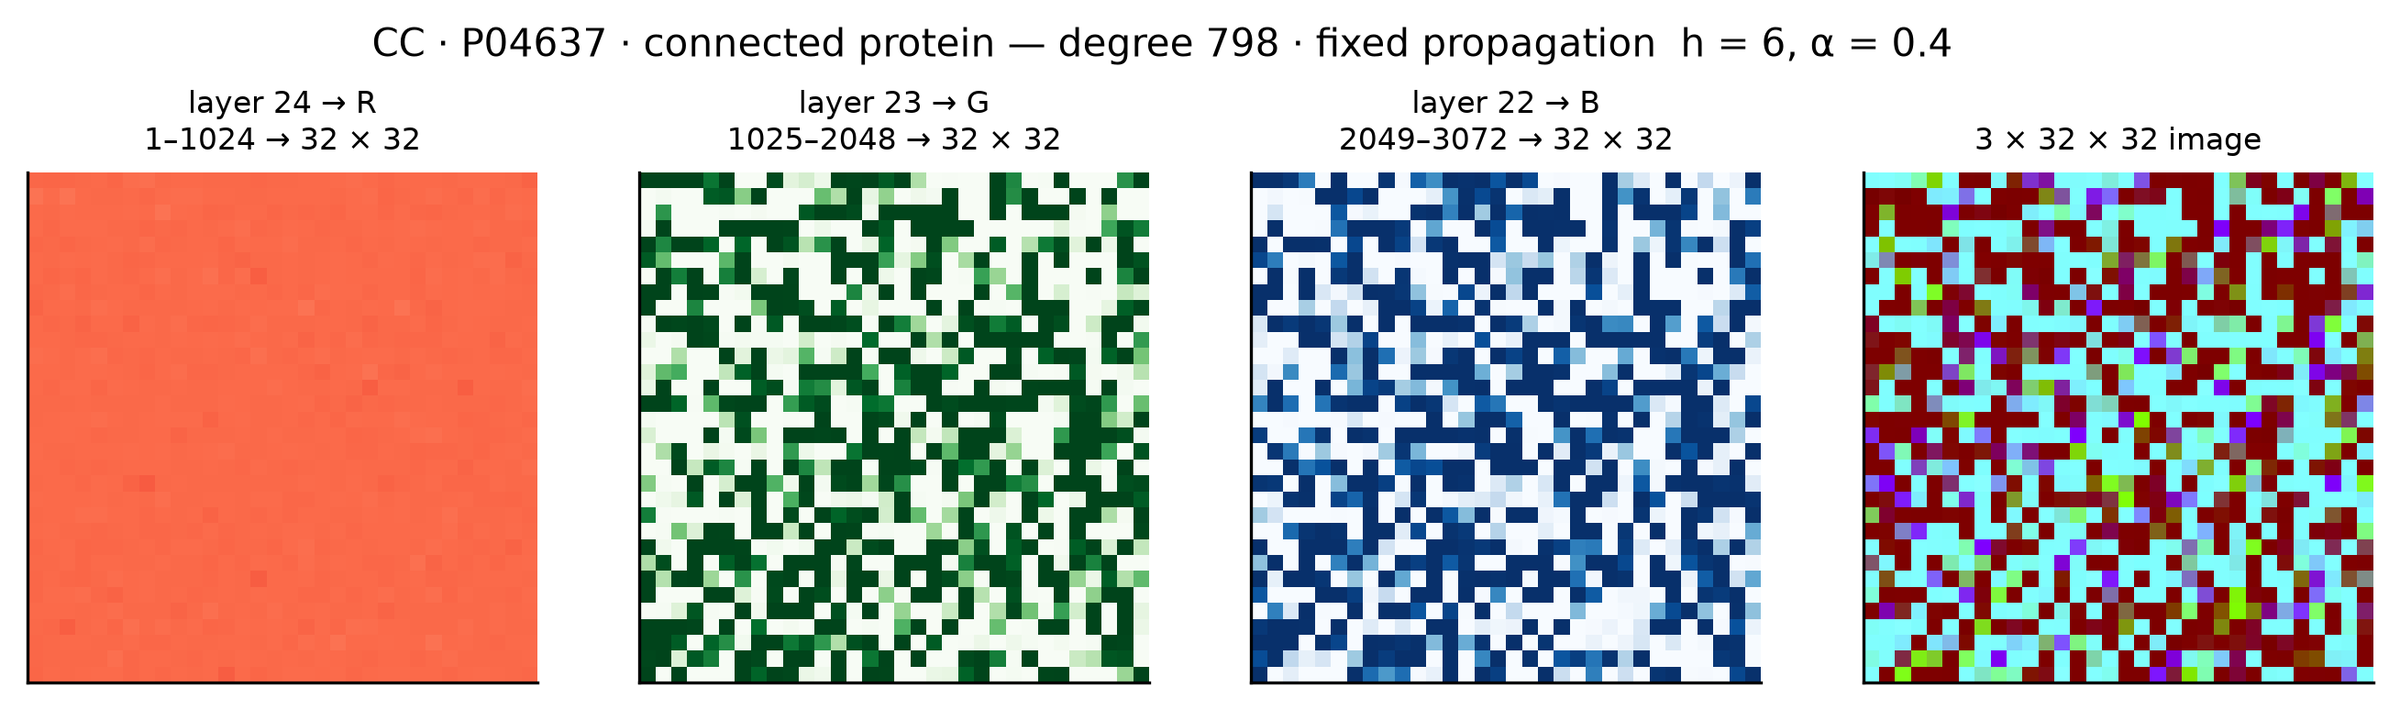
\includegraphics[width=1115.5\px,height=330\px]{figures/fig_5_9.png}};
\node[tl] at (88,70) {\fmR\fz{16}{16}\color{inkii}\ls{2}\Ll{4 · Method}};
\node[tl] at (88,131) {\fdA\fz{54}{56.7}\color{ink}\ls{-1}\Ll{Vector head and vision head}};
\node<3-5>[tl] at (88,603) {\fmR\fz{15}{19.5}\color{muted}\Ll{Dissertation, Fig. 5.9}};
\node<2-5>[tl] at (124,657.5) {\fbR\fz{26}{35.1}\color{ink}\Ll{Vector: MLP [1024, 512], batch norm, dropout 0.4}};
\node<4-5>[tl] at (856,657.5) {\fbR\fz{26}{35.1}\color{ink}\Ll{Backbones: ResNet-50 and ConvNeXt-Tiny (ImageNet),\\fully fine-tuned}};
\node<3-5>[tl] at (124,759.8) {\fbR\fz{26}{35.1}\color{ink}\Ll{Vision: {\fz{29.2}{35}$\sigma(\mathrm{clip}(z))$} split into three 32 × 32 channels, one\\per ProtT5 layer}};
\node<5>[tl] at (856,759.8) {\fbR\fz{26}{35.1}\color{ink}\Ll{Caution: pixel adjacency has no meaning here}};
\node[tr] at (1512,876) {\fmR\fz{16}{16}\color{muted}27 / 45};
\end{tikzpicture}
\note{The image is built inside the forward pass and never written to disk. 

Neighbouring pixels are neighbouring embedding coordinates only by storage order, a caveat that the results confirm.}
\end{frame}

\begin{frame}[plain]
\begin{tikzpicture}[deck]
\node<1-2>[box] at (0,0) {\includegraphics[page=3,width=1600\px]{build/layers}};
\node<3>[box] at (0,0) {\includegraphics[page=89,width=1600\px]{build/layers}};
\node<4>[box] at (0,0) {\includegraphics[page=90,width=1600\px]{build/layers}};
\node<5>[box] at (0,0) {\includegraphics[page=91,width=1600\px]{build/layers}};
\node[tl] at (88,70) {\fmR\fz{16}{16}\color{inkii}\ls{2}\Ll{4 · Method}};
\node[tl] at (88,131) {\fdA\fz{54}{56.7}\color{ink}\ls{-1}\Ll{Training objective: ProteinLoss}};
\node<2-5>[tl] at (88,251.7) {\fbR\fz{44}{52.8}\color{ink}\Ll{{\fz{49.4}{59.2}$\displaystyle \mathcal{L} = \mathcal{L}_{\text{ZLPR}} \cdot \bigl(1 - \mathrm{wF}_1^{\text{GO}}\bigr) \cdot \bigl(1 - \mathrm{wF}_1^{\text{prot}}\bigr)$}}};
\node<3-5>[tl] at (124,335) {\fbR\fz{30}{40.5}\color{ink}\Ll{ZLPR separates positive from negative\\terms at threshold zero}};
\node<4-5>[tl] at (124,438) {\fbR\fz{30}{40.5}\color{ink}\Ll{Two soft, IC-weighted {\fz{33.7}{40.4}$F_1$} factors: one\\across terms, one across proteins}};
\node<5>[tl] at (124,541) {\fbR\fz{30}{40.5}\color{ink}\Ll{Brings training closer to the\\evaluation criterion}};
\node[tr] at (1512,876) {\fmR\fz{16}{16}\color{muted}28 / 45};
\end{tikzpicture}
\note{Inherited from InterLabelGO+ through the group's sequence-only line. 

It beats binary cross-entropy by 5.47 pp on the first-generation mean, so every later run uses it.}
\end{frame}

\begin{frame}[plain]
\begin{tikzpicture}[deck]
\node<1>[box] at (0,0) {\includegraphics[page=3,width=1600\px]{build/layers}};
\node<2>[box] at (0,0) {\includegraphics[page=92,width=1600\px]{build/layers}};
\node<3>[box] at (0,0) {\includegraphics[page=93,width=1600\px]{build/layers}};
\node<4>[box] at (0,0) {\includegraphics[page=94,width=1600\px]{build/layers}};
\node<5>[box] at (0,0) {\includegraphics[page=95,width=1600\px]{build/layers}};
\node<6>[box] at (0,0) {\includegraphics[page=96,width=1600\px]{build/layers}};
\node<2-6>[box] at (109,235) {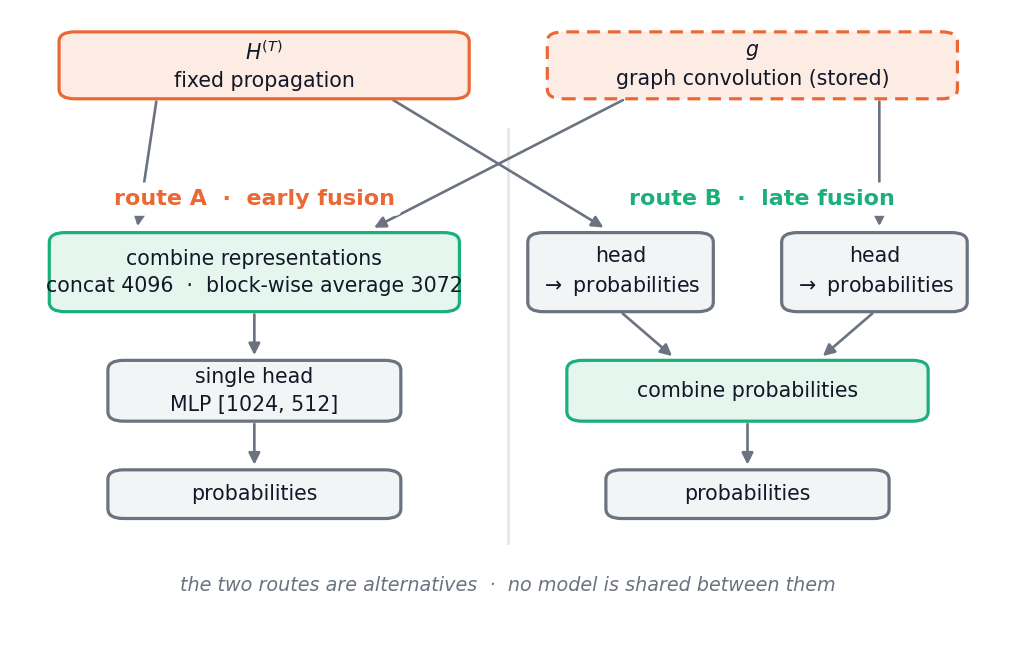
\includegraphics[width=654\px,height=417.1\px]{figures/fig_5_10.png}};
\node[tl] at (88,70) {\fmR\fz{16}{16}\color{inkii}\ls{2}\Ll{4 · Method}};
\node[tl] at (88,131) {\fdA\fz{54}{56.7}\color{ink}\ls{-1}\Ll{Combining the fixed and learned routes}};
\node<2-6>[tl] at (88,690.1) {\fmR\fz{15}{19.5}\color{muted}\Ll{Dissertation, Fig. 5.10}};
\node<3-6>[tl] at (852,232) {\fbR\fz{26}{35.1}\color{ink}\Ll{Early: join representations, train one head (concat 4096\\or block-wise add 3072)}};
\node<4-6>[tl] at (852,318.2) {\fbR\fz{26}{35.1}\color{ink}\Ll{Late: train each route, combine probabilities}};
\node<5-6>[tl] at (852,369.3) {\fbR\fz{26}{35.1}\color{ink}\Ll{Eleven late rules: linear {\fz{29.2}{35}$\gamma$}, max, min, IC sigmoid, degree\\sigmoid, master equation, five stacking meta-classifiers}};
\node<6>[tl] at (852,455.5) {\fbR\fz{26}{35.1}\color{ink}\Ll{Coefficients chosen on validation (71 configurations\\per ontology)}};
\node[tr] at (1512,876) {\fmR\fz{16}{16}\color{muted}29 / 45};
\end{tikzpicture}
\note{The two routes are alternatives, no model is shared. 

Early fusion lets one head learn how to weigh the sources; late fusion leaves each route to its own optimization and needs no training to combine.}
\end{frame}

\section{5 · Results}
\begin{frame}[plain]
\begin{tikzpicture}[deck]
\node<1>[box] at (0,0) {\includegraphics[page=3,width=1600\px]{build/layers}};
\node<2>[box] at (0,0) {\includegraphics[page=7,width=1600\px]{build/layers}};
\node<3>[box] at (0,0) {\includegraphics[page=97,width=1600\px]{build/layers}};
\node<4>[box] at (0,0) {\includegraphics[page=98,width=1600\px]{build/layers}};
\node[tl] at (88,70) {\fmR\fz{16}{16}\color{inkii}\ls{2}\Ll{5 · Results}};
\node[tl] at (88,131) {\fdA\fz{54}{56.7}\color{ink}\ls{-1}\Ll{170 runs, one funnel}};
\node<2-4>[tl] at (124,236) {\fbR\fz{30}{40.5}\color{ink}\Ll{170 runs, about 136.3 GPU-\\hours (147 on an RTX A5500)}};
\node<3-4>[tl] at (612,236) {\fbR\fz{30}{40.5}\color{ink}\Ll{Each stage picks its winner on\\validation and hands it on}};
\node<4>[tl] at (1100,236) {\fbR\fz{30}{40.5}\color{ink}\Ll{Test read once, at the end}};
\node[tr] at (1512,876) {\fmR\fz{16}{16}\color{muted}30 / 45};
\end{tikzpicture}
\note{The selection never touches the test partition. Every reported test number is a single evaluation of a frozen configuration. 

Two stations are not pure validation picks: max deduplication rests on an analytic argument (all 170 runs use it; the sum figures come from the earlier campaign), and ConvNeXt-Tiny is carried forward on a 0.57 pp margin plus the VISAPP campaign.}
\end{frame}

\begin{frame}[plain]
\begin{tikzpicture}[deck]
\node<1>[box] at (0,0) {\includegraphics[page=99,width=1600\px]{build/layers}};
\node<2>[box] at (0,0) {\includegraphics[page=100,width=1600\px]{build/layers}};
\node<3>[box] at (0,0) {\includegraphics[page=101,width=1600\px]{build/layers}};
\node<4>[box] at (0,0) {\includegraphics[page=102,width=1600\px]{build/layers}};
\node<5>[box] at (0,0) {\includegraphics[page=103,width=1600\px]{build/layers}};
\node[tl] at (88,70) {\fmR\fz{16}{16}\color{inkii}\ls{2}\Ll{5 · Results}};
\node[tl] at (88,131) {\fdA\fz{54}{56.7}\color{ink}\ls{-1}\Ll{Generation 1 settles three choices}};
\node<2-5>[tl] at (124,232) {\fbR\fz{26}{35.1}\color{ink}\Ll{Naive term-frequency baseline: 43.56\\mean wF\textsubscript{max}}};
\node<3-5>[tl] at (124,318.2) {\fbR\fz{26}{35.1}\color{ink}\Ll{ProteinLoss beats binary cross-entropy: +5.47\\pp mean (+8.87 in MF)}};
\node<4-5>[tl] at (124,404.4) {\fbR\fz{26}{35.1}\color{ink}\Ll{MLP on the raw profile wins: 44.51; best 1-D\\CNN 41.16}};
\node<5>[tl] at (124,490.6) {\fbR\fz{26}{35.1}\color{ink}\Ll{Vision backbones: 36.99 to 37.62}};
\node[tr] at (1512,876) {\fmR\fz{16}{16}\color{muted}31 / 45};
\end{tikzpicture}
\note{Topology alone barely clears a predictor that looks at nothing: 0.95 pp on the mean, and below it in BP. 

The vector route wins, and ConvNeXt-Tiny is carried forward on a 0.57 pp margin plus the earlier VISAPP campaign.}
\end{frame}

\begin{frame}[plain]
\begin{tikzpicture}[deck]
\node<1>[box] at (0,0) {\includegraphics[page=3,width=1600\px]{build/layers}};
\node<2>[box] at (0,0) {\includegraphics[page=104,width=1600\px]{build/layers}};
\node<3>[box] at (0,0) {\includegraphics[page=105,width=1600\px]{build/layers}};
\node<4>[box] at (0,0) {\includegraphics[page=106,width=1600\px]{build/layers}};
\node<2-4>[box] at (159.6,235) {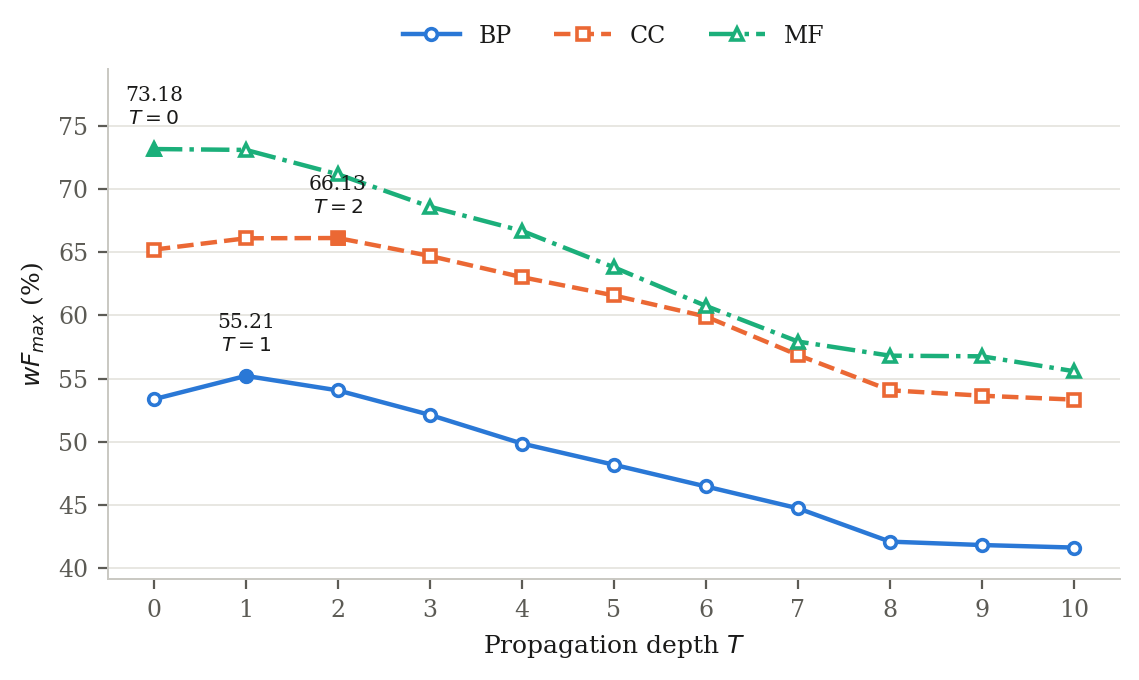
\includegraphics[width=552.8\px,height=330\px]{figures/fig_6_1.png}};
\node<3-4>[box] at (887.6,235) {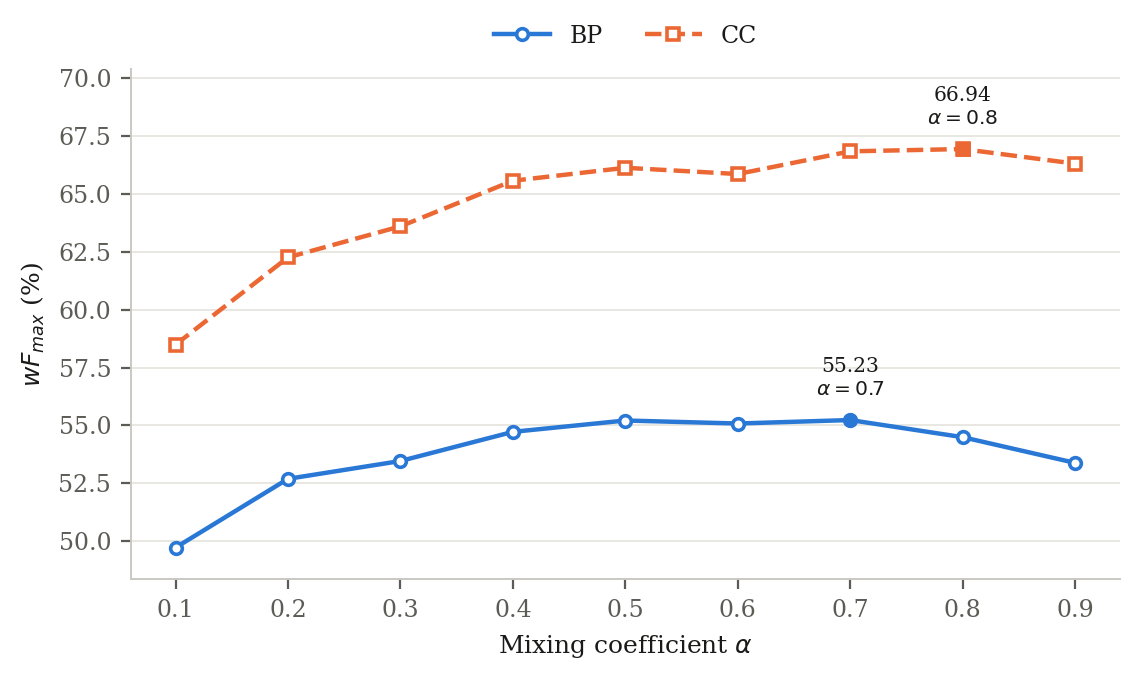
\includegraphics[width=552.8\px,height=330\px]{figures/fig_6_2.png}};
\node[tl] at (88,70) {\fmR\fz{16}{16}\color{inkii}\ls{2}\Ll{5 · Results}};
\node[tl] at (88,131) {\fdA\fz{54}{56.7}\color{ink}\ls{-1}\Ll{One or two hops, high retention}};
\node<2-4>[tl] at (88,603) {\fmR\fz{15}{19.5}\color{muted}\Ll{Dissertation, Fig. 6.1 · vector head, depth, validation}};
\node<3-4>[tl] at (816,603) {\fmR\fz{15}{19.5}\color{muted}\Ll{Dissertation, Fig. 6.2 · vector head, retention, validation}};
\node<2-4>[tl] at (124,655.5) {\fbR\fz{26}{35.1}\color{ink}\Ll{Peak depth: {\fz{29.2}{35}$T = 1$} BP, {\fz{29.2}{35}$T = 2$} CC, {\fz{29.2}{35}$T = 0$} MF}};
\node<3-4>[tl] at (852,655.5) {\fbR\fz{26}{35.1}\color{ink}\Ll{Best retention: {\fz{29.2}{35}$\alpha = 0.7$} BP, {\fz{29.2}{35}$\alpha = 0.8$} CC}};
\node<2-4>[tl] at (124,741.2) {\fbR\fz{26}{35.1}\color{ink}\Ll{Beyond the peak, performance falls 12.80 to 17.60 pp\\by {\fz{29.2}{35}$T = 10$}}};
\node<4>[tl] at (852,741.2) {\fbR\fz{26}{35.1}\color{ink}\Ll{The graph corrects the protein's own representation; it\\does not replace it}};
\node[tr] at (1512,876) {\fmR\fz{16}{16}\color{muted}32 / 45};
\end{tikzpicture}
\note{In MF no amount of propagation helps; the best configuration switches the graph off. 

In CC everything below $\alpha$ = 0.4 is worse than everything above it; in BP the single exception is $\alpha$ = 0.9.}
\end{frame}

\begin{frame}[plain]
\begin{tikzpicture}[deck]
\node<1>[box] at (0,0) {\includegraphics[page=3,width=1600\px]{build/layers}};
\node<2>[box] at (0,0) {\includegraphics[page=107,width=1600\px]{build/layers}};
\node<3>[box] at (0,0) {\includegraphics[page=108,width=1600\px]{build/layers}};
\node<4>[box] at (0,0) {\includegraphics[page=109,width=1600\px]{build/layers}};
\node<2-4>[box] at (159.6,235) {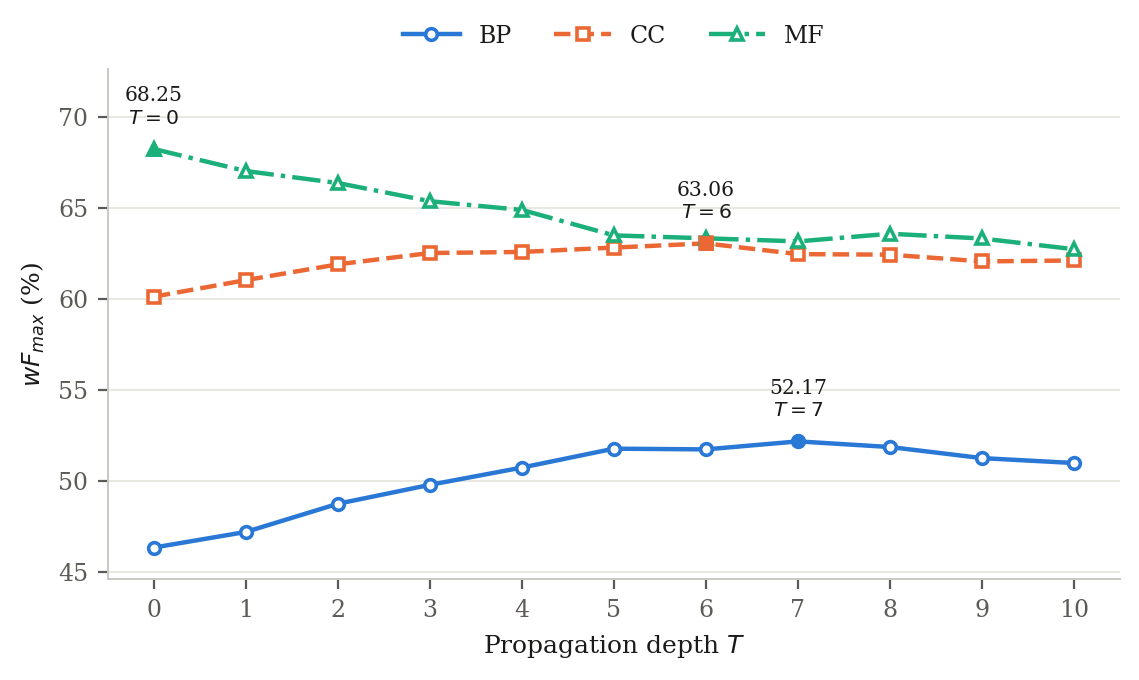
\includegraphics[width=552.8\px,height=330\px]{figures/fig_6_3.png}};
\node<3-4>[box] at (887.6,235) {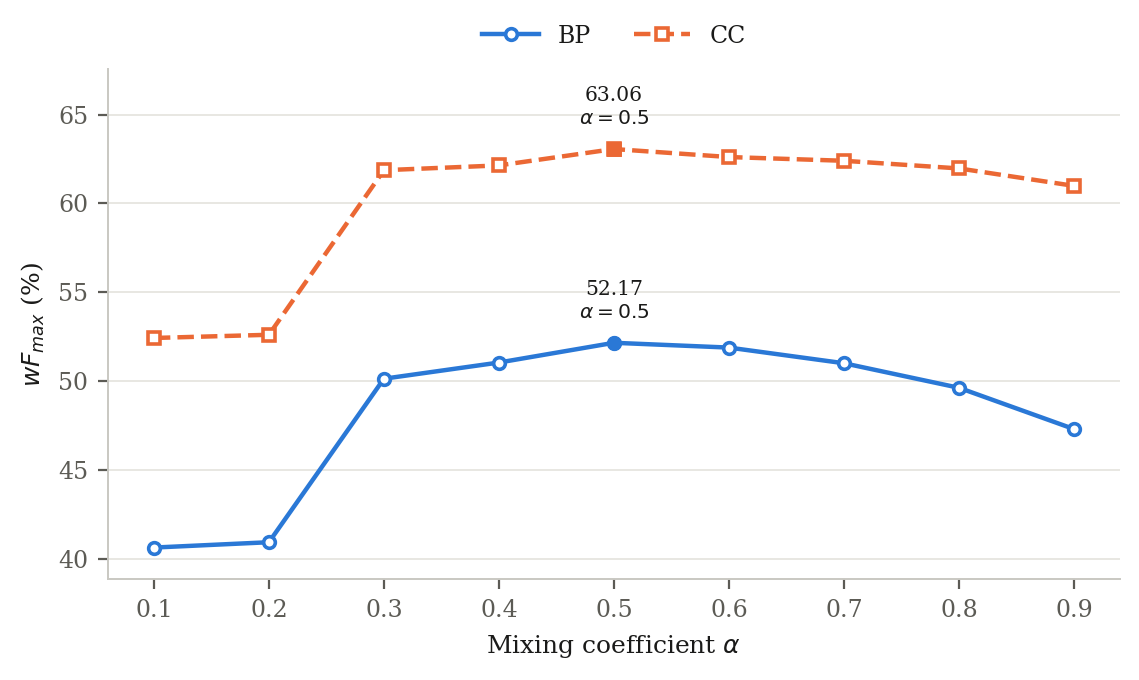
\includegraphics[width=552.8\px,height=330\px]{figures/fig_6_4.png}};
\node[tl] at (88,70) {\fmR\fz{16}{16}\color{inkii}\ls{2}\Ll{5 · Results}};
\node[tl] at (88,131) {\fdA\fz{54}{56.7}\color{ink}\ls{-1}\Ll{The vision head wants deep propagation}};
\node<2-4>[tl] at (88,603) {\fmR\fz{15}{19.5}\color{muted}\Ll{Dissertation, Fig. 6.3 · vision head, depth, validation}};
\node<3-4>[tl] at (816,603) {\fmR\fz{15}{19.5}\color{muted}\Ll{Dissertation, Fig. 6.4 · vision head, retention, validation}};
\node<2-4>[tl] at (124,655.5) {\fbR\fz{26}{35.1}\color{ink}\Ll{Peak depth: {\fz{29.2}{35}$T = 7$} BP, {\fz{29.2}{35}$T = 6$} CC, {\fz{29.2}{35}$T = 0$} MF; a plateau,\\not a peak}};
\node<3-4>[tl] at (852,655.5) {\fbR\fz{26}{35.1}\color{ink}\Ll{Collapse at {\fz{29.2}{35}$\alpha \le 0.2$}: isolated nodes shrink as {\fz{29.2}{35}$\alpha^{T}$} ({\fz{29.2}{35}$10^{-7}$}\\at {\fz{29.2}{35}$T = 7$})}};
\node<2-4>[tl] at (124,758.8) {\fbR\fz{26}{35.1}\color{ink}\Ll{Gains over {\fz{29.2}{35}$T = 0$}: +5.84 BP, +2.93 CC (vector head:\\+1.85, +0.92)}};
\node<4>[tl] at (852,758.8) {\fbR\fz{26}{35.1}\color{ink}\Ll{Its best BP value, 52.17, is still below the vector head's\\graph-free 53.36}};
\node[tr] at (1512,876) {\fmR\fz{16}{16}\color{muted}33 / 45};
\end{tikzpicture}
\note{The vision head extracts less from the node itself, so dilution costs it less and the neighbourhood average helps more. 

MF peaks at T = 0 in both heads, the strongest form of that observation.}
\end{frame}

\begin{frame}[plain]
\begin{tikzpicture}[deck]
\node<1>[box] at (0,0) {\includegraphics[page=110,width=1600\px]{build/layers}};
\node<2>[box] at (0,0) {\includegraphics[page=111,width=1600\px]{build/layers}};
\node<3>[box] at (0,0) {\includegraphics[page=112,width=1600\px]{build/layers}};
\node<4>[box] at (0,0) {\includegraphics[page=113,width=1600\px]{build/layers}};
\node<5>[box] at (0,0) {\includegraphics[page=114,width=1600\px]{build/layers}};
\node[tl] at (88,70) {\fmR\fz{16}{16}\color{inkii}\ls{2}\Ll{5 · Results}};
\node[tl] at (88,131) {\fdA\fz{54}{56.7}\color{ink}\ls{-1}\Ll{Learning the aggregation does not pay}};
\node<2-5>[tl] at (124,232) {\fbR\fz{26}{35.1}\color{ink}\Ll{GCN beats GAT in all 6 pairs (3.88 to 9.31 pp),\\and in 30 of 30 fusion pairs}};
\node<3-5>[tl] at (124,318.2) {\fbR\fz{26}{35.1}\color{ink}\Ll{Fixed 65.12 vs GCN 63.32 mean wF\textsubscript{max}}};
\node<4-5>[tl] at (124,369.3) {\fbR\fz{26}{35.1}\color{ink}\Ll{GCN ahead in BP by 0.55 (a tie); behind in CC\\by 0.59 and MF by 5.35}};
\node<5>[tl] at (124,455.5) {\fbR\fz{26}{35.1}\color{ink}\Ll{Deduplication: max never loses beyond noise;\\GAT gains most (+3.83 vision)}};
\node[tr] at (1512,876) {\fmR\fz{16}{16}\color{muted}34 / 45};
\end{tikzpicture}
\note{Attention does not recover a better weighting than the STRING score it was handed. 

A plausible reason: the loss is masked to training nodes, so attention parameters see gradient only through a two-hop receptive field.}
\end{frame}

\begin{frame}[plain]
\begin{tikzpicture}[deck]
\node<1>[box] at (0,0) {\includegraphics[page=115,width=1600\px]{build/layers}};
\node<2>[box] at (0,0) {\includegraphics[page=116,width=1600\px]{build/layers}};
\node<3>[box] at (0,0) {\includegraphics[page=117,width=1600\px]{build/layers}};
\node<4>[box] at (0,0) {\includegraphics[page=118,width=1600\px]{build/layers}};
\node<5>[box] at (0,0) {\includegraphics[page=119,width=1600\px]{build/layers}};
\node[tl] at (88,70) {\fmR\fz{16}{16}\color{inkii}\ls{2}\Ll{5 · Results}};
\node[tl] at (88,131) {\fdA\fz{54}{56.7}\color{ink}\ls{-1}\Ll{Fusion helps; combining predictions helps more}};
\node<2-5>[tl] at (124,232) {\fbR\fz{26}{35.1}\color{ink}\Ll{Early, one configuration (add, GCN, vector):\\65.80, +0.68 over fixed alone}};
\node<3-5>[tl] at (124,318.2) {\fbR\fz{26}{35.1}\color{ink}\Ll{Late, linear {\fz{29.2}{35}$\gamma$} (0.50 BP, 0.55 CC and MF):\\67.06, best in every ontology}};
\node<4-5>[tl] at (124,404.4) {\fbR\fz{26}{35.1}\color{ink}\Ll{Gains over the better component: +2.18 BP,\\+1.85 CC, +1.26 MF}};
\node<5>[tl] at (124,490.6) {\fbR\fz{26}{35.1}\color{ink}\Ll{Stacking importances: the two probabilities\\carry almost all the weight}};
\node[tr] at (1512,876) {\fmR\fz{16}{16}\color{muted}35 / 45};
\end{tikzpicture}
\note{A single scalar beats every elaborate rule, including gradient boosting. The auxiliary features do not predict which route is right, and the conditional rules converged to the flattest sigmoid in the grid. 

The ensemble fits one extra parameter on validation.}
\end{frame}

\begin{frame}[plain]
\begin{tikzpicture}[deck]
\node<1>[box] at (0,0) {\includegraphics[page=120,width=1600\px]{build/layers}};
\node<2>[box] at (0,0) {\includegraphics[page=121,width=1600\px]{build/layers}};
\node<3>[box] at (0,0) {\includegraphics[page=122,width=1600\px]{build/layers}};
\node<4>[box] at (0,0) {\includegraphics[page=123,width=1600\px]{build/layers}};
\node[tl] at (88,70) {\fmR\fz{16}{16}\color{inkii}\ls{2}\Ll{5 · Results}};
\node[tl] at (88,131) {\fdA\fz{54}{56.7}\color{ink}\ls{-1}\Ll{Vector head wins 12 of 12}};
\node<3-4>[tl] at (1094.7,232) {\fbR\fz{26}{35.1}\color{ink}\Ll{Margin on the mean: +6.62,\\+3.96, +2.69, +3.35 pp across the\\four stages}};
\node<3-4>[tl] at (1094.7,353.3) {\fbR\fz{26}{35.1}\color{ink}\Ll{No trend toward zero}};
\node<4>[tl] at (1094.7,404.4) {\fbR\fz{26}{35.1}\color{ink}\Ll{Neither image has the locality a\\convolution assumes}};
\node[tr] at (1512,876) {\fmR\fz{16}{16}\color{muted}36 / 45};
\end{tikzpicture}
\note{Generation 1 images index arbitrary training proteins; generation 2 images reshape embedding coordinates. 

Three independent pieces of evidence agree: pooling order, the 1-D CNN failure and this table.}
\end{frame}

\begin{frame}[plain]
\begin{tikzpicture}[deck]
\node<1>[box] at (0,0) {\includegraphics[page=124,width=1600\px]{build/layers}};
\node<2>[box] at (0,0) {\includegraphics[page=125,width=1600\px]{build/layers}};
\node<3>[box] at (0,0) {\includegraphics[page=126,width=1600\px]{build/layers}};
\node<4>[box] at (0,0) {\includegraphics[page=127,width=1600\px]{build/layers}};
\node<5>[box] at (0,0) {\includegraphics[page=128,width=1600\px]{build/layers}};
\node[tl] at (88,70) {\fmR\fz{16}{16}\color{inkii}\ls{2}\Ll{5 · Results}};
\node[tl] at (88,131) {\fdA\fz{54}{56.7}\color{ink}\ls{-1}\Ll{Where the gains come from}};
\node<4-5>[tl] at (124,688) {\fbR\fz{26}{35.1}\color{ink}\Ll{Mean validation wF\textsubscript{max}: Naive 43.56 $\rightarrow$ Generation 1 44.51 $\rightarrow$ ProtT5 alone 63.92 $\rightarrow$ Fixed 65.12 $\rightarrow$ Early 65.84 $\rightarrow$\\Late 67.06}};
\node<5>[tl] at (124,774.2) {\fbR\fz{26}{35.1}\color{ink}\Ll{Most of the jump is the language model; the graph adds the rest}};
\node[tr] at (1512,876) {\fmR\fz{16}{16}\color{muted}37 / 45};
\end{tikzpicture}
\note{This is the whole dissertation on one axis. The protein language model explains most of the distance, and the graph contributes a consistent remainder in BP and CC. 

Each value is a mean of per-ontology champions on validation; the learned GNN alone, 63.32, sits below the ProtT5 control because of MF, so it is not a step of the staircase.}
\end{frame}

\begin{frame}[plain]
\hypertarget<1>{s38.1}{}
\hypertarget<2>{s38.2}{}
\hypertarget<3>{s38.3}{}
\hypertarget<4>{s38.4}{}
\hypertarget<5>{s38.5}{}
\hypertarget<6>{s38.6}{}
\hypertarget<7>{s38.7}{}
\begin{tikzpicture}[deck]
\node<1>[box] at (0,0) {\includegraphics[page=129,width=1600\px]{build/layers}};
\node<2>[box] at (0,0) {\includegraphics[page=130,width=1600\px]{build/layers}};
\node<3>[box] at (0,0) {\includegraphics[page=131,width=1600\px]{build/layers}};
\node<4>[box] at (0,0) {\includegraphics[page=132,width=1600\px]{build/layers}};
\node<5>[box] at (0,0) {\includegraphics[page=133,width=1600\px]{build/layers}};
\node<6>[box] at (0,0) {\includegraphics[page=134,width=1600\px]{build/layers}};
\node<7>[box] at (0,0) {\includegraphics[page=135,width=1600\px]{build/layers}};
\node<5>[box] at (787.5,208) {\hot{58.1}{42}{s38.5}};
\node<5>[box] at (844.1,208) {\hot{59.4}{42}{s38.6}};
\node<5>[box] at (902,208) {\hot{61.5}{42}{s38.7}};
\node<5>[box] at (1049.1,206) {\hot{227}{46}{s38x.4}};
\node<6>[box] at (787.5,208) {\hot{58.1}{42}{s38.5}};
\node<6>[box] at (844.1,208) {\hot{59.4}{42}{s38.6}};
\node<6>[box] at (902,208) {\hot{61.5}{42}{s38.7}};
\node<6>[box] at (1049.1,206) {\hot{227}{46}{s38x.10}};
\node<7>[box] at (787.5,208) {\hot{58.1}{42}{s38.5}};
\node<7>[box] at (844.1,208) {\hot{59.4}{42}{s38.6}};
\node<7>[box] at (902,208) {\hot{61.5}{42}{s38.7}};
\node<7>[box] at (1049.1,206) {\hot{227}{46}{s38x.16}};
\node[tl] at (88,70) {\fmR\fz{16}{16}\color{inkii}\ls{2}\Ll{5 · Results}};
\node[tl] at (88,131) {\fdA\fz{54}{56.7}\color{ink}\ls{-1}\Ll{Test set: NEXUS-GO vs five methods}};
\node<2-7>[tl] at (124,232) {\fbR\fz{26}{35.1}\color{ink}\Ll{NEXUS-GO/Late best in every column of the\\three tables, except AuPRC in MF}};
\node<3-7>[tl] at (124,318.2) {\fbR\fz{26}{35.1}\color{ink}\Ll{wF\textsubscript{max} margin over the strongest baseline:\\+9.77 BP, +8.67 CC, +4.93 MF}};
\node<4-7>[tl] at (124,404.4) {\fbR\fz{26}{35.1}\color{ink}\Ll{S\textsubscript{min}: 17.12 vs 20.11 (BP), 8.22 vs 9.67 (CC), 5.14\\vs 5.67 (MF)}};
\node<5-7>[tl] at (124,490.6) {\fbR\fz{26}{35.1}\color{ink}\Ll{The ProtT5 baseline alone already beats every\\literature method on wF\textsubscript{max}}};
\node[tr] at (1512,876) {\fmR\fz{16}{16}\color{muted}38 / 45};
\end{tikzpicture}
\note{Every baseline was retrained on the same corpus and scored with the same code. 

Three of them lose their multi-network mechanism on a single aggregated graph, so the ordering describes these adapted configurations, not the original papers.}
\end{frame}

\begin{frame}[plain]
\begin{tikzpicture}[deck]
\node<1>[box] at (0,0) {\includegraphics[page=136,width=1600\px]{build/layers}};
\node<2>[box] at (0,0) {\includegraphics[page=137,width=1600\px]{build/layers}};
\node<3>[box] at (0,0) {\includegraphics[page=138,width=1600\px]{build/layers}};
\node[tl] at (88,70) {\fmR\fz{16}{16}\color{inkii}\ls{2}\Ll{5 · Results}};
\node[tl] at (88,131) {\fdA\fz{54}{56.7}\color{ink}\ls{-1}\Ll{Every protein gets a prediction}};
\node<2-3>[tl] at (124,236) {\fbR\fz{30}{40.5}\color{ink}\Ll{NEXUS-GO: 100\% of the test partition in\\BP, CC, MF}};
\node<3>[tl] at (124,339) {\fbR\fz{30}{40.5}\color{ink}\Ll{DeepGraphGO and SEGT-GO: 95.1–\\96.3\% (homology search)}};
\node<3>[tl] at (124,442) {\fbR\fz{30}{40.5}\color{ink}\Ll{Mashup, MELISSA, deepNF: 63.6–68.7\%\\(network members only)}};
\node[tr] at (1512,876) {\fmR\fz{16}{16}\color{muted}39 / 45};
\end{tikzpicture}
\note{Missing proteins count as misses in the comparison, so part of the distance to the network-only methods is reach, not ranking quality. 

The proteins they cannot reach are exactly the band where sequence-aware routes score highest.}
\end{frame}

\begin{frame}[plain]
\begin{tikzpicture}[deck]
\node<1>[box] at (0,0) {\includegraphics[page=3,width=1600\px]{build/layers}};
\node<2>[box] at (0,0) {\includegraphics[page=139,width=1600\px]{build/layers}};
\node<3>[box] at (0,0) {\includegraphics[page=140,width=1600\px]{build/layers}};
\node<4>[box] at (0,0) {\includegraphics[page=141,width=1600\px]{build/layers}};
\node<5>[box] at (0,0) {\includegraphics[page=142,width=1600\px]{build/layers}};
\node<2-5>[box] at (109,235) {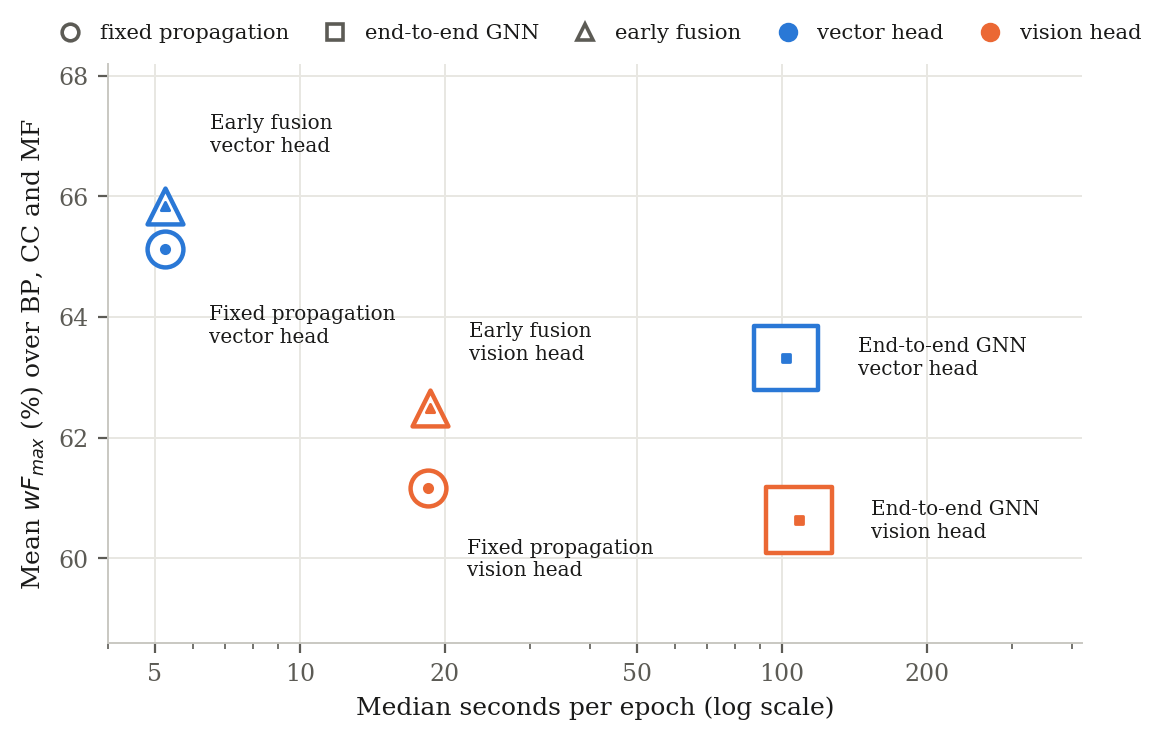
\includegraphics[width=654\px,height=415.4\px]{figures/fig_6_5.png}};
\node[tl] at (88,70) {\fmR\fz{16}{16}\color{inkii}\ls{2}\Ll{5 · Results}};
\node[tl] at (88,131) {\fdA\fz{54}{56.7}\color{ink}\ls{-1}\Ll{A thirteenth of the time per epoch}};
\node<2-5>[tl] at (88,688.4) {\fmR\fz{15}{19.5}\color{muted}\Ll{Dissertation, Fig. 6.5}};
\node<3-5>[tl] at (852,232) {\fbR\fz{26}{35.1}\color{ink}\Ll{Fixed + vector: 5.24 s/epoch, 6.4 GiB peak}};
\node<3-5>[tl] at (852,283.1) {\fbR\fz{26}{35.1}\color{ink}\Ll{GCN alone: 68.76 s/epoch, 14.1 GiB; GAT 161.41 s,\\20.7 GiB}};
\node<4-5>[tl] at (852,369.3) {\fbR\fz{26}{35.1}\color{ink}\Ll{{\fbB{}Matches or beats the GCN at about 1/13 of the time}\\{\fbB{}and under half the memory}}};
\node<5>[tl] at (852,455.5) {\fbR\fz{26}{35.1}\color{ink}\Ll{Early fusion costs the same as fixed propagation once {\fz{29.2}{35}$\mathbf{g}$}\\is stored}};
\node[tr] at (1512,876) {\fmR\fz{16}{16}\color{muted}40 / 45};
\end{tikzpicture}
\note{The fixed operator runs once per experiment; the learned ones recompute a full-graph propagation at every optimization step. 

Early-fusion cost excludes training the GCN checkpoint it consumes.}
\end{frame}

\begin{frame}[plain]
\begin{tikzpicture}[deck]
\node<1>[box] at (0,0) {\includegraphics[page=3,width=1600\px]{build/layers}};
\node<2>[box] at (0,0) {\includegraphics[page=143,width=1600\px]{build/layers}};
\node<3>[box] at (0,0) {\includegraphics[page=144,width=1600\px]{build/layers}};
\node<4>[box] at (0,0) {\includegraphics[page=145,width=1600\px]{build/layers}};
\node<2-4>[box] at (109,235) {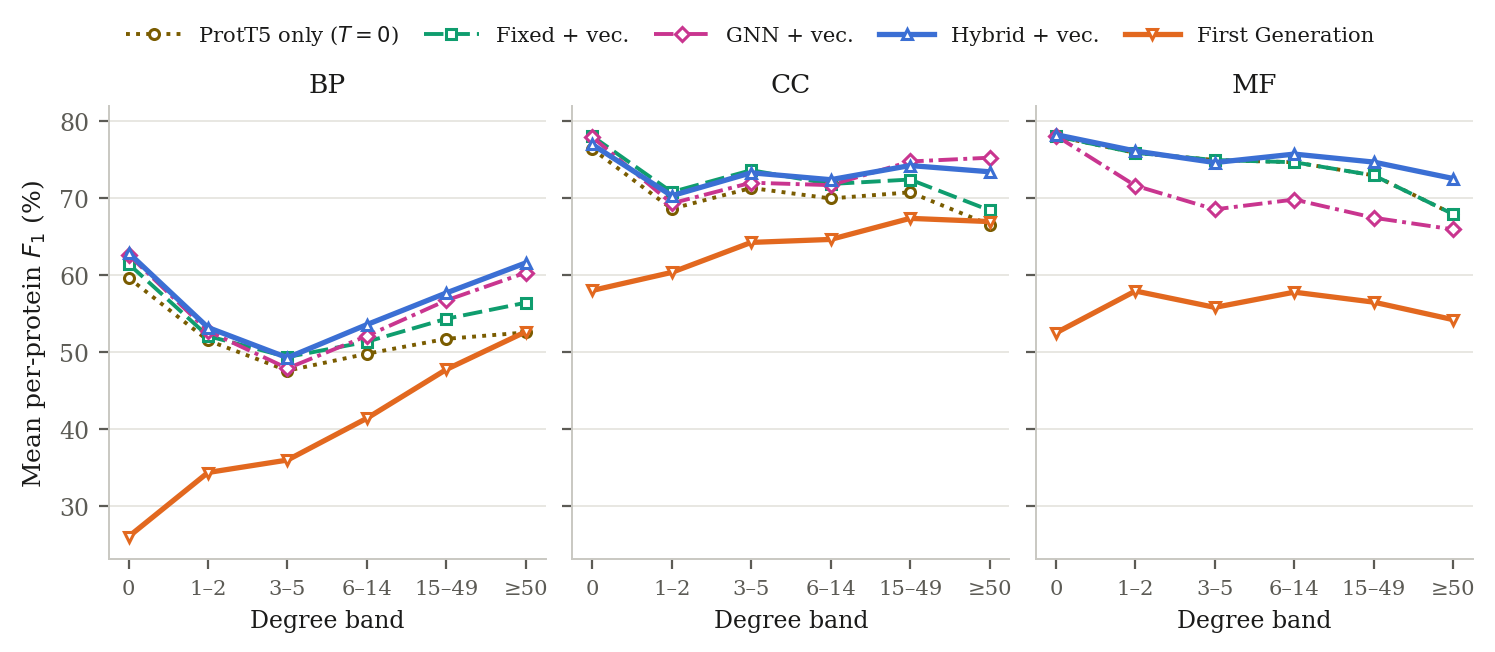
\includegraphics[width=802.5\px,height=350\px]{figures/fig_6_6.png}};
\node[tl] at (88,70) {\fmR\fz{16}{16}\color{inkii}\ls{2}\Ll{5 · Results}};
\node[tl] at (88,131) {\fdA\fz{54}{56.7}\color{ink}\ls{-1}\Ll{The graph helps where there is graph}};
\node<2-4>[tl] at (88,623) {\fmR\fz{15}{19.5}\color{muted}\Ll{Dissertation, Fig. 6.6 · test}};
\node<3-4>[tl] at (1094.7,232) {\fbR\fz{26}{35.1}\color{ink}\Ll{Every ProtT5 route scores worse on\\connected than on isolated proteins}};
\node<3-4>[tl] at (1094.7,318.2) {\fbR\fz{26}{35.1}\color{ink}\Ll{The graph-free control already\\shows it, so the graph does not\\cause it}};
\node<4>[tl] at (1094.7,439.5) {\fbR\fz{26}{35.1}\color{ink}\Ll{The graph's gain grows with degree:\\up to +9.05 BP, +8.71 CC, +4.64 MF\\at degree $\geq$ 50}};
\node[tr] at (1512,876) {\fmR\fz{16}{16}\color{muted}41 / 45};
\end{tikzpicture}
\note{Hubs tend to be multifunctional and harder for a sequence model. In BP the hardest proteins have degree 3 to 5, not zero. 

Degree-zero differences come from rescaling and refitting, so read topological gains from degree one upward.}
\end{frame}

\section{6 · Conclusions}
\begin{frame}[plain]
\begin{tikzpicture}[deck]
\node<1>[box] at (0,0) {\includegraphics[page=3,width=1600\px]{build/layers}};
\node<2>[box] at (0,0) {\includegraphics[page=146,width=1600\px]{build/layers}};
\node<3>[box] at (0,0) {\includegraphics[page=147,width=1600\px]{build/layers}};
\node<4>[box] at (0,0) {\includegraphics[page=148,width=1600\px]{build/layers}};
\node[tl] at (88,70) {\fmR\fz{16}{16}\color{inkii}\ls{2}\Ll{6 · Conclusions}};
\node[tl] at (88,131) {\fdA\fz{54}{56.7}\color{ink}\ls{-1}\Ll{Answers to the research questions}};
\node<2-4>[tc] at (126,232) {\fmM\fz{20}{20}\color{ink}\Lc{RQ1}};
\node<2-4>[tl] at (184,232) {\fbR\fz{20}{26}\color{inkii}\Ll{Which network representation works best?}};
\node<2-4>[tl] at (184,266) {\fbR\fz{27}{35.1}\color{ink}\Ll{The unreduced profile and an MLP; imposed locality hurts}};
\node<2-4>[tc] at (126,321.1) {\fmM\fz{20}{20}\color{ink}\Lc{RQ2}};
\node<2-4>[tl] at (184,321.1) {\fbR\fz{20}{26}\color{inkii}\Ll{How much does propagating ProtT5 over STRING add?}};
\node<2-4>[tl] at (184,355.1) {\fbR\fz{27}{35.1}\color{ink}\Ll{Large gain, mostly from ProtT5; propagation adds +1.87 BP, +2.15 CC, nothing in MF (test)}};
\node<2-4>[tc] at (126,410.2) {\fmM\fz{20}{20}\color{ink}\Lc{RQ3}};
\node<2-4>[tl] at (184,410.2) {\fbR\fz{20}{26}\color{inkii}\Ll{Fixed vs learned aggregation, vector vs image heads}};
\node<2-4>[tl] at (184,444.2) {\fbR\fz{27}{35.1}\color{ink}\Ll{Late 67.06 > Early 65.84 > Fixed 65.12 > GNN 63.32 (validation); vector head throughout}};
\node<3-4>[tc] at (126,499.3) {\fmM\fz{20}{20}\color{ink}\Lc{RQ4}};
\node<3-4>[tl] at (184,499.3) {\fbR\fz{20}{26}\color{inkii}\Ll{Do early and late fusion help?}};
\node<3-4>[tl] at (184,533.3) {\fbR\fz{27}{35.1}\color{ink}\Ll{Both help; late more (+1.26 to +2.18 pp, validation)}};
\node<3-4>[tc] at (126,588.4) {\fmM\fz{20}{20}\color{ink}\Lc{RQ5}};
\node<3-4>[tl] at (184,588.4) {\fbR\fz{20}{26}\color{inkii}\Ll{How deep, and how much retention?}};
\node<3-4>[tl] at (184,622.4) {\fbR\fz{27}{35.1}\color{ink}\Ll{One or two hops, {\fz{30.3}{36.3}$\alpha$} 0.7 to 0.8; MF prefers none}};
\node<4>[tc] at (126,677.5) {\fmM\fz{20}{20}\color{ink}\Lc{RQ6}};
\node<4>[tl] at (184,677.5) {\fbR\fz{20}{26}\color{inkii}\Ll{How does it compare with the literature?}};
\node<4>[tl] at (184,711.5) {\fbR\fz{27}{35.1}\color{ink}\Ll{Best in every column but one; +9.77 / +8.67 / +4.93 pp wF\textsubscript{max} (test)}};
\node<4>[tc] at (126,766.6) {\fmM\fz{20}{20}\color{ink}\Lc{RQ7}};
\node<4>[tl] at (184,766.6) {\fbR\fz{20}{26}\color{inkii}\Ll{Does it work on one global, aggregated network?}};
\node<4>[tl] at (184,800.6) {\fbR\fz{27}{35.1}\color{ink}\Ll{Works on one global aggregated network; partitioned graphs not tested}};
\node[tr] at (1512,876) {\fmR\fz{16}{16}\color{muted}42 / 45};
\end{tikzpicture}
\note{Use the conclusions chapter wording if asked for detail. 

RQ7 is applicability, not superiority over partitioned graphs.}
\end{frame}

\begin{frame}[plain]
\begin{tikzpicture}[deck]
\node<1>[box] at (0,0) {\includegraphics[page=3,width=1600\px]{build/layers}};
\node<2>[box] at (0,0) {\includegraphics[page=149,width=1600\px]{build/layers}};
\node<3>[box] at (0,0) {\includegraphics[page=150,width=1600\px]{build/layers}};
\node<4>[box] at (0,0) {\includegraphics[page=151,width=1600\px]{build/layers}};
\node[tl] at (88,70) {\fmR\fz{16}{16}\color{inkii}\ls{2}\Ll{6 · Conclusions}};
\node[tl] at (88,131) {\fdA\fz{54}{56.7}\color{ink}\ls{-1}\Ll{Limitations}};
\node<2-4>[tl] at (124,236) {\fbR\fz{30}{40.5}\color{ink}\Ll{Single seed; the 0.5 pp floor is a reading convention, not a confidence interval}};
\node<2-4>[tl] at (124,298.5) {\fbR\fz{30}{40.5}\color{ink}\Ll{Random protein-level split: transductive interpolation, possible homology leakage}};
\node<3-4>[tl] at (124,361) {\fbR\fz{30}{40.5}\color{ink}\Ll{STRING scores may encode annotation knowledge (circularity)}};
\node<4>[tl] at (124,423.5) {\fbR\fz{30}{40.5}\color{ink}\Ll{Fixed vs learned is not a single-factor ablation ({\fz{33.7}{40.4}$\alpha^{T}$} scaling, normalization)}};
\node<4>[tl] at (124,486) {\fbR\fz{30}{40.5}\color{ink}\Ll{Baselines adapted to one aggregated network and a reduced label space}};
\node[tr] at (1512,876) {\fmR\fz{16}{16}\color{muted}43 / 45};
\end{tikzpicture}
\note{State these before the committee does. 

Each one is documented in the dissertation with its consequence.}
\end{frame}

\begin{frame}[plain]
\begin{tikzpicture}[deck]
\node<1>[box] at (0,0) {\includegraphics[page=3,width=1600\px]{build/layers}};
\node<2>[box] at (0,0) {\includegraphics[page=152,width=1600\px]{build/layers}};
\node<3>[box] at (0,0) {\includegraphics[page=153,width=1600\px]{build/layers}};
\node[tl] at (88,70) {\fmR\fz{16}{16}\color{inkii}\ls{2}\Ll{6 · Conclusions}};
\node[tl] at (88,131) {\fdA\fz{54}{56.7}\color{ink}\ls{-1}\Ll{Next steps}};
\node<2-3>[tl] at (115,337) {\fbR\fz{27}{35.1}\color{ink}\Ll{Separate the graph by organism,\\or one model per organism}};
\node<2-3>[tl] at (599,337) {\fbR\fz{27}{35.1}\color{ink}\Ll{Keep STRING evidence channels\\apart (typed or parallel edges)}};
\node<2-3>[tl] at (1083,337) {\fbR\fz{27}{35.1}\color{ink}\Ll{Heterogeneous graphs (proteins,\\terms, evidence); compare with\\ProtHGT}};
\node<3>[tl] at (357,604.3) {\fbR\fz{27}{35.1}\color{ink}\Ll{Sampled aggregation\\(GraphSAGE) for a cheaper\\learned route}};
\node<3>[tl] at (841,604.3) {\fbR\fz{27}{35.1}\color{ink}\Ll{Richer node features: structure,\\domains, expression; most\\promising for MF}};
\node[tr] at (1512,876) {\fmR\fz{16}{16}\color{muted}44 / 45};
\end{tikzpicture}
\note{The two most immediate are taxonomic scope and evidence channels. 

MF is where the network contributed least, so new node features matter most there.}
\end{frame}

\begin{frame}[plain]
\begin{tikzpicture}[deck]
\node[box] at (0,0) {\includegraphics[page=154,width=1600\px]{build/layers}};
\node[tl] at (88,367) {\fdB\fz{104}{98.8}\color{ink}\ls{-2.5}\Ll{Thank you}};
\node[tl] at (124,412.8) {\fbR\fz{30}{40.5}\color{ink}\Ll{NEXUS-GO: fixed propagation of ProtT5 over STRING, fused with a GCN, best in every\\ontology at a fraction of the cost}};
\node[tl] at (124,515.8) {\fbR\fz{30}{40.5}\color{ink}\Ll{Code: {\fmR\fz{25.8}{31}{}github.com/ymauhn/nexus-go}}};
\node[tl] at (124,578.3) {\fbR\fz{30}{40.5}\color{ink}\Ll{Publications: VISAPP 2026; extended version accepted in CCIS (expected December 2026)}};
\node[tl] at (124,640.8) {\fbR\fz{30}{40.5}\color{ink}\Ll{Funding: CAPES, BTG Pactual · Computing resources: IC/Unicamp}};
\node[tl] at (88,829) {\fdA\fz{40}{40}\color{ink}\Ll{Questions}};
\end{tikzpicture}
\note{Thank the committee, the advisors and the funders. 

Open for questions.}
\end{frame}

\section{Backup}
\begin{frame}[plain]
\begin{tikzpicture}[deck]
\node[box] at (0,0) {\includegraphics[page=155,width=1600\px]{build/layers}};
\node[tl] at (88,70) {\fmR\fz{16}{16}\color{inkii}\ls{2}\Ll{Backup}};
\node[tl] at (88,131) {\fdA\fz{54}{56.7}\color{ink}\ls{-1}\Ll{Hyperparameters}};
\node[tl] at (100,230) {\fbB\fz{20}{24}\color{inkii}\Ll{Setting}};
\node[tl] at (320.5,230) {\fbB\fz{20}{24}\color{inkii}\Ll{Value}};
\node[tl] at (499,230) {\fbB\fz{20}{24}\color{inkii}\Ll{Scope}};
\node[tl] at (100,264) {\fbR\fz{18}{21.6}\color{ink}\Ll{Optimizer}};
\node[tl] at (320.5,264) {\fbR\fz{18}{21.6}\color{ink}\Ll{Adam}};
\node[tl] at (499,264) {\fbR\fz{18}{21.6}\color{ink}\Ll{all families}};
\node[tl] at (100,299) {\fbR\fz{18}{21.6}\color{ink}\Ll{Learning rate}};
\node[tl] at (320.5,299) {\fbR\fz{18}{21.6}\color{ink}\Ll{1 × 10\textsuperscript{-4}}};
\node[tl] at (499,299) {\fbR\fz{18}{21.6}\color{ink}\Ll{all families}};
\node[tl] at (100,334) {\fbR\fz{18}{21.6}\color{ink}\Ll{Weight decay}};
\node[tl] at (320.5,334) {\fbR\fz{18}{21.6}\color{ink}\Ll{none}};
\node[tl] at (499,334) {\fbR\fz{18}{21.6}\color{ink}\Ll{all families}};
\node[tl] at (100,369) {\fbR\fz{18}{21.6}\color{ink}\Ll{Learning-rate schedule}};
\node[tl] at (320.5,369) {\fbR\fz{18}{21.6}\color{ink}\Ll{none}};
\node[tl] at (499,369) {\fbR\fz{18}{21.6}\color{ink}\Ll{all families}};
\node[tl] at (100,404) {\fbR\fz{18}{21.6}\color{ink}\Ll{Batch size}};
\node[tl] at (320.5,404) {\fbR\fz{18}{21.6}\color{ink}\Ll{256}};
\node[tl] at (499,404) {\fbR\fz{18}{21.6}\color{ink}\Ll{all families}};
\node[tl] at (100,439) {\fbR\fz{18}{21.6}\color{ink}\Ll{Maximum epochs}};
\node[tl] at (320.5,439) {\fbR\fz{18}{21.6}\color{ink}\Ll{250}};
\node[tl] at (499,439) {\fbR\fz{18}{21.6}\color{ink}\Ll{all families}};
\node[tl] at (100,474) {\fbR\fz{18}{21.6}\color{ink}\Ll{Early-stopping patience}};
\node[tl] at (320.5,474) {\fbR\fz{18}{21.6}\color{ink}\Ll{20 epochs}};
\node[tl] at (499,474) {\fbR\fz{18}{21.6}\color{ink}\Ll{all families}};
\node[tl] at (100,509) {\fbR\fz{18}{21.6}\color{ink}\Ll{Monitored quantity}};
\node[tl] at (320.5,509) {\fbR\fz{18}{21.6}\color{ink}\Ll{validation loss}};
\node[tl] at (499,509) {\fbR\fz{18}{21.6}\color{ink}\Ll{all families}};
\node[tl] at (100,544) {\fbR\fz{18}{21.6}\color{ink}\Ll{Minimum improvement}};
\node[tl] at (320.5,544) {\fbR\fz{18}{21.6}\color{ink}\Ll{0}};
\node[tl] at (499,544) {\fbR\fz{18}{21.6}\color{ink}\Ll{all families}};
\node[tl] at (100,579) {\fbR\fz{18}{21.6}\color{ink}\Ll{Objective}};
\node[tl] at (320.5,579) {\fbR\fz{18}{21.6}\color{ink}\Ll{Eq. 5.20}};
\node[tl] at (499,579) {\fbR\fz{18}{21.6}\color{ink}\Ll{all families}};
\node[tl] at (100,614) {\fbR\fz{18}{21.6}\color{ink}\Ll{Class weighting}};
\node[tl] at (320.5,614) {\fbR\fz{18}{21.6}\color{ink}\Ll{information content}};
\node[tl] at (499,614) {\fbR\fz{18}{21.6}\color{ink}\Ll{all families}};
\node[tl] at (100,649) {\fbR\fz{18}{21.6}\color{ink}\Ll{Dropout, prediction head}};
\node[tl] at (320.5,649) {\fbR\fz{18}{21.6}\color{ink}\Ll{0.4}};
\node[tl] at (499,649) {\fbR\fz{18}{21.6}\color{ink}\Ll{all families}};
\node[tl] at (88,686) {\fmR\fz{15}{19.5}\color{muted}\Ll{Dissertation, Table A.2}};
\node[tl] at (828,230) {\fbB\fz{20}{24}\color{inkii}\Ll{Setting}};
\node[tl] at (1072.2,230) {\fbB\fz{20}{24}\color{inkii}\Ll{Value}};
\node[tl] at (1359,230) {\fbB\fz{20}{24}\color{inkii}\Ll{Scope}};
\node[tl] at (828,264) {\fbR\fz{18}{24}\color{ink}\Ll{Dropout, between\\convolutions}};
\node[tl] at (1072.2,264) {\fbR\fz{18}{21.6}\color{ink}\Ll{0.3}};
\node[tl] at (1359,264) {\fbR\fz{18}{24}\color{ink}\Ll{graph\\convolutions}};
\node[tl] at (828,323) {\fbR\fz{18}{21.6}\color{ink}\Ll{Hidden widths, head}};
\node[tl] at (1072.2,323) {\fbR\fz{18}{21.6}\color{ink}\Ll{[1024, 512]}};
\node[tl] at (1359,323) {\fbR\fz{18}{21.6}\color{ink}\Ll{all families}};
\node[tl] at (828,358) {\fbR\fz{18}{21.6}\color{ink}\Ll{Convolution hidden width}};
\node[tl] at (1072.2,358) {\fbR\fz{18}{21.6}\color{ink}\Ll{1024}};
\node[tl] at (1359,358) {\fbR\fz{18}{24}\color{ink}\Ll{graph\\convolutions}};
\node[tl] at (828,417) {\fbR\fz{18}{21.6}\color{ink}\Ll{Convolution layers}};
\node[tl] at (1072.2,417) {\fbR\fz{18}{21.6}\color{ink}\Ll{2}};
\node[tl] at (1359,417) {\fbR\fz{18}{24}\color{ink}\Ll{graph\\convolutions}};
\node[tl] at (828,476) {\fbR\fz{18}{21.6}\color{ink}\Ll{Attention heads}};
\node[tl] at (1072.2,476) {\fbR\fz{18}{21.6}\color{ink}\Ll{4 (hidden), 1 (output)}};
\node[tl] at (1359,476) {\fbR\fz{18}{21.6}\color{ink}\Ll{graph attention}};
\node[tl] at (828,511) {\fbR\fz{18}{21.6}\color{ink}\Ll{Random seed}};
\node[tl] at (1072.2,511) {\fbR\fz{18}{21.6}\color{ink}\Ll{1337}};
\node[tl] at (1359,511) {\fbR\fz{18}{21.6}\color{ink}\Ll{all families}};
\node[tl] at (828,546) {\fbR\fz{18}{21.6}\color{ink}\Ll{Data-loading workers}};
\node[tl] at (1072.2,546) {\fbR\fz{18}{21.6}\color{ink}\Ll{4}};
\node[tl] at (1359,546) {\fbR\fz{18}{21.6}\color{ink}\Ll{all families}};
\node[tl] at (828,581) {\fbR\fz{18}{21.6}\color{ink}\Ll{Configured edge threshold}};
\node[tl] at (1072.2,581) {\fbR\fz{18}{24}\color{ink}\Ll{0.10 (inert; source-data floor =\\0.400)}};
\node[tl] at (1359,581) {\fbR\fz{18}{21.6}\color{ink}\Ll{all families}};
\node[tl] at (828,640) {\fbR\fz{18}{21.6}\color{ink}\Ll{Propagation steps T}};
\node[tl] at (1072.2,640) {\fbR\fz{18}{21.6}\color{ink}\Ll{varies}};
\node[tl] at (1359,640) {\fbR\fz{18}{21.6}\color{ink}\Ll{fixed propagation}};
\node[tl] at (828,676) {\fbR\fz{18}{21.6}\color{ink}\Ll{Mixing coefficient $\alpha$}};
\node[tl] at (1072.2,675) {\fbR\fz{18}{21.6}\color{ink}\Ll{varies}};
\node[tl] at (1359,675) {\fbR\fz{18}{21.6}\color{ink}\Ll{fixed propagation}};
\node[tl] at (828,711) {\fbR\fz{18}{21.6}\color{ink}\Ll{Deduplication rule}};
\node[tl] at (1072.2,711) {\fbR\fz{18}{21.6}\color{ink}\Ll{varies}};
\node[tl] at (1359,711) {\fbR\fz{18}{21.6}\color{ink}\Ll{all families}};
\node[tl] at (816,748) {\fmR\fz{15}{19.5}\color{muted}\Ll{Dissertation, Table A.2}};
\node[tr] at (1512,876) {\fmR\fz{16}{16}\color{muted}B1};
\end{tikzpicture}
\note{Optimization settings of the final second-generation campaign (Table A.2). Values marked varies are part of the search space.}
\end{frame}

\begin{frame}[plain]
\begin{tikzpicture}[deck]
\node[box] at (0,0) {\includegraphics[page=156,width=1600\px]{build/layers}};
\node[tl] at (88,70) {\fmR\fz{16}{16}\color{inkii}\ls{2}\Ll{Backup}};
\node[tl] at (88,131) {\fdA\fz{54}{56.7}\color{ink}\ls{-1}\Ll{Late fusion: grid and selected coefficients}};
\node[tl] at (100,230) {\fbB\fz{20}{24}\color{inkii}\Ll{Rule}};
\node[tl] at (381.2,230) {\fbB\fz{20}{24}\color{inkii}\Ll{Grid}};
\node[tl] at (826.4,230) {\fbB\fz{20}{24}\color{inkii}\Ll{Config.}};
\node[tl] at (100,264) {\fbR\fz{18}{21.6}\color{ink}\Ll{Linear combination}};
\node[tl] at (381.2,265) {\fbR\fz{18}{21.6}\color{ink}\Ll{$\gamma$ from 0.00 to 1.00 in steps of 0.05}};
\node[tl] at (826.4,264) {\fbR\fz{18}{21.6}\color{ink}\Ll{21}};
\node[tl] at (100,300) {\fbR\fz{18}{24}\color{ink}\Ll{Pointwise maximum and\\minimum}};
\node[tl] at (381.2,300) {\fbR\fz{18}{21.6}\color{ink}\Ll{no parameter}};
\node[tl] at (826.4,300) {\fbR\fz{18}{21.6}\color{ink}\Ll{2}};
\node[tl] at (100,359) {\fbR\fz{18}{21.6}\color{ink}\Ll{Term-specific weighting}};
\node[tl] at (381.2,360) {\fbR\fz{18}{21.6}\color{ink}\Ll{IC\textsubscript{thr} $\in$ \{0.4, 1.1, 2.1, 3.4\} and $\kappa$\textsubscript{IC} $\in$ \{1, 2, 5\}}};
\node[tl] at (826.4,359) {\fbR\fz{18}{21.6}\color{ink}\Ll{12}};
\node[tl] at (100,395) {\fbR\fz{18}{21.6}\color{ink}\Ll{Protein-specific weighting}};
\node[tl] at (381.2,396) {\fbR\fz{18}{24}\color{ink}\Ll{d\textsubscript{thr} $\in$ \{1, 3, 5, 14, 28\} and $\kappa$\textsubscript{deg} $\in$ \{0.25, 0.50, 0.75,\\1.00\}}};
\node[tl] at (826.4,395) {\fbR\fz{18}{21.6}\color{ink}\Ll{20}};
\node[tl] at (100,455) {\fbR\fz{18}{21.6}\color{ink}\Ll{Combined weighting}};
\node[tl] at (381.2,456) {\fbR\fz{18}{21.6}\color{ink}\Ll{$\lambda$ from 0.0 to 1.0 in steps of 0.1}};
\node[tl] at (826.4,455) {\fbR\fz{18}{21.6}\color{ink}\Ll{11}};
\node[tl] at (100,491) {\fbR\fz{18}{21.6}\color{ink}\Ll{Stacking}};
\node[tl] at (381.2,491) {\fbR\fz{18}{21.6}\color{ink}\Ll{five meta-classifiers, no coefficient swept}};
\node[tl] at (826.4,491) {\fbR\fz{18}{21.6}\color{ink}\Ll{5}};
\node[tl] at (100,526) {\fbR\fz{18}{21.6}\color{ink}\Ll{Total}};
\node[tl] at (826.4,526) {\fbR\fz{18}{21.6}\color{ink}\Ll{71}};
\node[tl] at (88,563) {\fmR\fz{15}{19.5}\color{muted}\Ll{Dissertation, Table A.3}};
\node[tl] at (949.3,230) {\fbB\fz{20}{24}\color{inkii}\Ll{Rule}};
\node[tr] at (1281.6,230) {\fbB\fz{20}{24}\color{inkii}\Lr{Coefficient}};
\node[tr] at (1348.8,230) {\fbB\fz{20}{24}\color{inkii}\Lr{BP}};
\node[tr] at (1416,230) {\fbB\fz{20}{24}\color{inkii}\Lr{CC}};
\node[tr] at (1483.2,230) {\fbB\fz{20}{24}\color{inkii}\Lr{MF}};
\node[tl] at (949.3,264) {\fbR\fz{18}{21.6}\color{ink}\Ll{Linear combination}};
\node[tr] at (1281.6,264.5) {\fmR\fz{18}{21.6}\color{ink}\Lr{$\gamma$}};
\node[tr] at (1348.8,264.5) {\fmR\fz{18}{21.6}\color{ink}\Lr{0.50}};
\node[tr] at (1416,264.5) {\fmR\fz{18}{21.6}\color{ink}\Lr{0.55}};
\node[tr] at (1483.2,264.5) {\fmR\fz{18}{21.6}\color{ink}\Lr{0.55}};
\node[tl] at (949.3,299) {\fbR\fz{18}{21.6}\color{ink}\Ll{Term-specific weighting}};
\node[tr] at (1281.6,299.5) {\fmR\fz{18}{21.6}\color{ink}\Lr{IC\textsubscript{thr}}};
\node[tr] at (1348.8,299.5) {\fmR\fz{18}{21.6}\color{ink}\Lr{1.1}};
\node[tr] at (1416,299.5) {\fmR\fz{18}{21.6}\color{ink}\Lr{0.4}};
\node[tr] at (1483.2,299.5) {\fmR\fz{18}{21.6}\color{ink}\Lr{0.4}};
\node[tr] at (1281.6,334) {\fmR\fz{18}{21.6}\color{ink}\Lr{$\kappa$\textsubscript{IC}}};
\node[tr] at (1348.8,334) {\fmR\fz{18}{21.6}\color{ink}\Lr{1.0}};
\node[tr] at (1416,334) {\fmR\fz{18}{21.6}\color{ink}\Lr{1.0}};
\node[tr] at (1483.2,334) {\fmR\fz{18}{21.6}\color{ink}\Lr{1.0}};
\node[tl] at (949.3,368) {\fbR\fz{18}{21.6}\color{ink}\Ll{Protein-specific weighting}};
\node[tr] at (1281.6,368.5) {\fmR\fz{18}{21.6}\color{ink}\Lr{d\textsubscript{thr}}};
\node[tr] at (1348.8,368.5) {\fmR\fz{18}{21.6}\color{ink}\Lr{3}};
\node[tr] at (1416,368.5) {\fmR\fz{18}{21.6}\color{ink}\Lr{14}};
\node[tr] at (1483.2,368.5) {\fmR\fz{18}{21.6}\color{ink}\Lr{28}};
\node[tr] at (1281.6,403) {\fmR\fz{18}{21.6}\color{ink}\Lr{$\kappa$\textsubscript{deg}}};
\node[tr] at (1348.8,403) {\fmR\fz{18}{21.6}\color{ink}\Lr{0.25}};
\node[tr] at (1416,403) {\fmR\fz{18}{21.6}\color{ink}\Lr{0.25}};
\node[tr] at (1483.2,403) {\fmR\fz{18}{21.6}\color{ink}\Lr{0.25}};
\node[tl] at (949.3,437) {\fbR\fz{18}{21.6}\color{ink}\Ll{Combined weighting}};
\node[tr] at (1281.6,437.5) {\fmR\fz{18}{21.6}\color{ink}\Lr{$\lambda$}};
\node[tr] at (1348.8,437.5) {\fmR\fz{18}{21.6}\color{ink}\Lr{0.5}};
\node[tr] at (1416,437.5) {\fmR\fz{18}{21.6}\color{ink}\Lr{0.4}};
\node[tr] at (1483.2,437.5) {\fmR\fz{18}{21.6}\color{ink}\Lr{0.9}};
\node[tl] at (937.3,474) {\fmR\fz{15}{19.5}\color{muted}\Ll{Dissertation, Table A.4}};
\node[tr] at (1512,876) {\fmR\fz{16}{16}\color{muted}B2};
\end{tikzpicture}
\note{71 configurations per ontology, chosen on validation. Both conditional rules converged on the flattest sigmoid the grid offers.}
\end{frame}

\begin{frame}[plain]
\begin{tikzpicture}[deck]
\node[box] at (0,0) {\includegraphics[page=157,width=1600\px]{build/layers}};
\node[tl] at (88,70) {\fmR\fz{16}{16}\color{inkii}\ls{2}\Ll{Backup}};
\node[tl] at (88,131) {\fdA\fz{54}{56.7}\color{ink}\ls{-1}\Ll{Early fusion: provenance × source}};
\node[tl] at (100,230) {\fbB\fz{20}{24}\color{inkii}\Ll{Head}};
\node[tr] at (239.5,230) {\fbB\fz{20}{24}\color{inkii}\Lr{Fusion}};
\node[tr] at (371,230) {\fbB\fz{20}{24}\color{inkii}\Lr{Provenance}};
\node[tr] at (459.8,230) {\fbB\fz{20}{24}\color{inkii}\Lr{Source}};
\node[tr] at (537.8,230) {\fbB\fz{20}{24}\color{inkii}\Lr{BP}};
\node[tr] at (615.8,230) {\fbB\fz{20}{24}\color{inkii}\Lr{CC}};
\node[tr] at (693.8,230) {\fbB\fz{20}{24}\color{inkii}\Lr{MF}};
\node[tl] at (100,264) {\fbR\fz{18}{21.6}\color{ink}\Ll{Vector}};
\node[tr] at (239.5,264.5) {\fmR\fz{18}{21.6}\color{ink}\Lr{add}};
\node[tr] at (371,264.5) {\fmR\fz{18}{21.6}\color{ink}\Lr{vector}};
\node[tr] at (459.8,264.5) {\fmR\fz{18}{21.6}\color{ink}\Lr{vector}};
\node[tr] at (537.8,264.5) {\fmR\fz{18}{21.6}\color{ink}\Lr{56.52}};
\node[tr] at (615.8,264.5) {\fmR\fz{18}{21.6}\color{ink}\Lr{66.86}};
\node[tr] at (693.8,264.5) {\fmR\fz{18}{21.6}\color{ink}\Lr{73.81}};
\node[tr] at (239.5,299) {\fmR\fz{18}{21.6}\color{ink}\Lr{add}};
\node[tr] at (371,299) {\fmR\fz{18}{21.6}\color{ink}\Lr{vector}};
\node[tr] at (459.8,299) {\fmR\fz{18}{21.6}\color{ink}\Lr{vision}};
\node[tr] at (537.8,299) {\fmR\fz{18}{21.6}\color{ink}\Lr{55.73}};
\node[tr] at (615.8,299) {\fmR\fz{18}{21.6}\color{ink}\Lr{65.79}};
\node[tr] at (693.8,299) {\fmR\fz{18}{21.6}\color{ink}\Lr{n/a}};
\node[tr] at (239.5,333) {\fmR\fz{18}{21.6}\color{ink}\Lr{add}};
\node[tr] at (371,333) {\fmR\fz{18}{21.6}\color{ink}\Lr{vision}};
\node[tr] at (459.8,333) {\fmR\fz{18}{21.6}\color{ink}\Lr{vector}};
\node[tr] at (537.8,333) {\fmR\fz{18}{21.6}\color{ink}\Lr{53.98}};
\node[tr] at (615.8,333) {\fmR\fz{18}{21.6}\color{ink}\Lr{67.07}};
\node[tr] at (693.8,333) {\fmR\fz{18}{21.6}\color{ink}\Lr{73.42}};
\node[tr] at (239.5,367) {\fmR\fz{18}{21.6}\color{ink}\Lr{add}};
\node[tr] at (371,367) {\fmR\fz{18}{21.6}\color{ink}\Lr{vision}};
\node[tr] at (459.8,367) {\fmR\fz{18}{21.6}\color{ink}\Lr{vision}};
\node[tr] at (537.8,367) {\fmR\fz{18}{21.6}\color{ink}\Lr{52.96}};
\node[tr] at (615.8,367) {\fmR\fz{18}{21.6}\color{ink}\Lr{65.46}};
\node[tr] at (693.8,367) {\fmR\fz{18}{21.6}\color{ink}\Lr{n/a}};
\node[tr] at (239.5,401) {\fmR\fz{18}{21.6}\color{ink}\Lr{concat}};
\node[tr] at (371,401) {\fmR\fz{18}{21.6}\color{ink}\Lr{vector}};
\node[tr] at (459.8,401) {\fmR\fz{18}{21.6}\color{ink}\Lr{vector}};
\node[tr] at (537.8,401) {\fmR\fz{18}{21.6}\color{ink}\Lr{56.05}};
\node[tr] at (615.8,401) {\fmR\fz{18}{21.6}\color{ink}\Lr{67.12}};
\node[tr] at (693.8,401) {\fmR\fz{18}{21.6}\color{ink}\Lr{73.68}};
\node[tr] at (239.5,435) {\fmR\fz{18}{21.6}\color{ink}\Lr{concat}};
\node[tr] at (371,435) {\fmR\fz{18}{21.6}\color{ink}\Lr{vector}};
\node[tr] at (459.8,435) {\fmR\fz{18}{21.6}\color{ink}\Lr{vision}};
\node[tr] at (537.8,435) {\fmR\fz{18}{21.6}\color{ink}\Lr{55.52}};
\node[tr] at (615.8,435) {\fmR\fz{18}{21.6}\color{ink}\Lr{65.27}};
\node[tr] at (693.8,435) {\fmR\fz{18}{21.6}\color{ink}\Lr{n/a}};
\node[tr] at (239.5,469) {\fmR\fz{18}{21.6}\color{ink}\Lr{concat}};
\node[tr] at (371,469) {\fmR\fz{18}{21.6}\color{ink}\Lr{vision}};
\node[tr] at (459.8,469) {\fmR\fz{18}{21.6}\color{ink}\Lr{vector}};
\node[tr] at (537.8,469) {\fmR\fz{18}{21.6}\color{ink}\Lr{55.32}};
\node[tr] at (615.8,469) {\fmR\fz{18}{21.6}\color{ink}\Lr{67.20}};
\node[tr] at (693.8,469) {\fmR\fz{18}{21.6}\color{ink}\Lr{73.78}};
\node[tr] at (239.5,503) {\fmR\fz{18}{21.6}\color{ink}\Lr{concat}};
\node[tr] at (371,503) {\fmR\fz{18}{21.6}\color{ink}\Lr{vision}};
\node[tr] at (459.8,503) {\fmR\fz{18}{21.6}\color{ink}\Lr{vision}};
\node[tr] at (537.8,503) {\fmR\fz{18}{21.6}\color{ink}\Lr{53.23}};
\node[tr] at (615.8,503) {\fmR\fz{18}{21.6}\color{ink}\Lr{65.42}};
\node[tr] at (693.8,503) {\fmR\fz{18}{21.6}\color{ink}\Lr{n/a}};
\node[tl] at (100,537) {\fbR\fz{18}{21.6}\color{ink}\Ll{Vision}};
\node[tr] at (239.5,537.5) {\fmR\fz{18}{21.6}\color{ink}\Lr{add}};
\node[tr] at (371,537.5) {\fmR\fz{18}{21.6}\color{ink}\Lr{vector}};
\node[tr] at (459.8,537.5) {\fmR\fz{18}{21.6}\color{ink}\Lr{vector}};
\node[tr] at (537.8,537.5) {\fmR\fz{18}{21.6}\color{ink}\Lr{52.36}};
\node[tr] at (615.8,537.5) {\fmR\fz{18}{21.6}\color{ink}\Lr{64.77}};
\node[tr] at (693.8,537.5) {\fmR\fz{18}{21.6}\color{ink}\Lr{69.52}};
\node[tr] at (239.5,572) {\fmR\fz{18}{21.6}\color{ink}\Lr{add}};
\node[tr] at (371,572) {\fmR\fz{18}{21.6}\color{ink}\Lr{vector}};
\node[tr] at (459.8,572) {\fmR\fz{18}{21.6}\color{ink}\Lr{vision}};
\node[tr] at (537.8,572) {\fmR\fz{18}{21.6}\color{ink}\Lr{53.17}};
\node[tr] at (615.8,572) {\fmR\fz{18}{21.6}\color{ink}\Lr{64.71}};
\node[tr] at (693.8,572) {\fmR\fz{18}{21.6}\color{ink}\Lr{n/a}};
\node[tr] at (239.5,606) {\fmR\fz{18}{21.6}\color{ink}\Lr{add}};
\node[tr] at (371,606) {\fmR\fz{18}{21.6}\color{ink}\Lr{vision}};
\node[tr] at (459.8,606) {\fmR\fz{18}{21.6}\color{ink}\Lr{vector}};
\node[tr] at (537.8,606) {\fmR\fz{18}{21.6}\color{ink}\Lr{49.72}};
\node[tr] at (615.8,606) {\fmR\fz{18}{21.6}\color{ink}\Lr{62.66}};
\node[tr] at (693.8,606) {\fmR\fz{18}{21.6}\color{ink}\Lr{67.66}};
\node[tr] at (239.5,640) {\fmR\fz{18}{21.6}\color{ink}\Lr{add}};
\node[tr] at (371,640) {\fmR\fz{18}{21.6}\color{ink}\Lr{vision}};
\node[tr] at (459.8,640) {\fmR\fz{18}{21.6}\color{ink}\Lr{vision}};
\node[tr] at (537.8,640) {\fmR\fz{18}{21.6}\color{ink}\Lr{50.21}};
\node[tr] at (615.8,640) {\fmR\fz{18}{21.6}\color{ink}\Lr{62.64}};
\node[tr] at (693.8,640) {\fmR\fz{18}{21.6}\color{ink}\Lr{n/a}};
\node[tl] at (88,676) {\fmR\fz{15}{19.5}\color{muted}\Ll{Dissertation, Table 6.13}};
\node[tr] at (1512,876) {\fmR\fz{16}{16}\color{muted}B3};
\end{tikzpicture}
\note{Provenance is the head with which the consumed GNN embedding was trained; source is the head whose depth and retention were used for the fixed branch. Validation set.}
\end{frame}

\begin{frame}[plain]
\begin{tikzpicture}[deck]
\node[box] at (0,0) {\includegraphics[page=158,width=1600\px]{build/layers}};
\node[tl] at (88,70) {\fmR\fz{16}{16}\color{inkii}\ls{2}\Ll{Backup}};
\node[tl] at (88,131) {\fdA\fz{54}{56.7}\color{ink}\ls{-1}\Ll{Isolated vs connected proteins}};
\node[tl] at (100,230) {\fbB\fz{20}{24}\color{inkii}\Ll{Route}};
\node[tr] at (601.1,230) {\fbB\fz{20}{24}\color{inkii}\Lr{BP}};
\node[tr] at (845.9,230) {\fbB\fz{20}{24}\color{inkii}\Lr{CC}};
\node[tr] at (1090.7,230) {\fbB\fz{20}{24}\color{inkii}\Lr{MF}};
\node[tr] at (434.3,265) {\fbB\fz{20}{24}\color{inkii}\Lr{Isol.}};
\node[tr] at (512.3,265) {\fbB\fz{20}{24}\color{inkii}\Lr{Conn.}};
\node[tr] at (601.1,265) {\fbB\fz{20}{24}\color{inkii}\Lr{$\Delta$}};
\node[tr] at (679.1,265) {\fbB\fz{20}{24}\color{inkii}\Lr{Isol.}};
\node[tr] at (757.1,265) {\fbB\fz{20}{24}\color{inkii}\Lr{Conn.}};
\node[tr] at (845.9,265) {\fbB\fz{20}{24}\color{inkii}\Lr{$\Delta$}};
\node[tr] at (923.9,265) {\fbB\fz{20}{24}\color{inkii}\Lr{Isol.}};
\node[tr] at (1001.9,265) {\fbB\fz{20}{24}\color{inkii}\Lr{Conn.}};
\node[tr] at (1090.7,265) {\fbB\fz{20}{24}\color{inkii}\Lr{$\Delta$}};
\node[tl] at (100,299) {\fbR\fz{18}{21.6}\color{ink}\Ll{ProtT5 only (T=0)}};
\node[tr] at (434.3,299.5) {\fmR\fz{18}{21.6}\color{ink}\Lr{59.89}};
\node[tr] at (512.3,299.5) {\fmR\fz{18}{21.6}\color{ink}\Lr{50.23}};
\node[tr] at (601.1,299.5) {\fmR\fz{18}{21.6}\color{ink}\Lr{−9.66}};
\node[tr] at (679.1,299.5) {\fmR\fz{18}{21.6}\color{ink}\Lr{69.30}};
\node[tr] at (757.1,299.5) {\fmR\fz{18}{21.6}\color{ink}\Lr{62.38}};
\node[tr] at (845.9,299.5) {\fmR\fz{18}{21.6}\color{ink}\Lr{−6.92}};
\node[tr] at (923.9,299.5) {\fmR\fz{18}{21.6}\color{ink}\Lr{75.68}};
\node[tr] at (1001.9,299.5) {\fmR\fz{18}{21.6}\color{ink}\Lr{71.23}};
\node[tr] at (1090.7,299.5) {\fmR\fz{18}{21.6}\color{ink}\Lr{−4.45}};
\node[tl] at (100,334) {\fbR\fz{18}{21.6}\color{ink}\Ll{Fixed propagation + vector head}};
\node[tr] at (434.3,334.5) {\fmR\fz{18}{21.6}\color{ink}\Lr{61.30}};
\node[tr] at (512.3,334.5) {\fmR\fz{18}{21.6}\color{ink}\Lr{52.39}};
\node[tr] at (601.1,334.5) {\fmR\fz{18}{21.6}\color{ink}\Lr{−8.91}};
\node[tr] at (679.1,334.5) {\fmR\fz{18}{21.6}\color{ink}\Lr{71.12}};
\node[tr] at (757.1,334.5) {\fmR\fz{18}{21.6}\color{ink}\Lr{64.77}};
\node[tr] at (845.9,334.5) {\fmR\fz{18}{21.6}\color{ink}\Lr{−6.35}};
\node[tr] at (923.9,334.5) {\fmR\fz{18}{21.6}\color{ink}\Lr{75.68}};
\node[tr] at (1001.9,334.5) {\fmR\fz{18}{21.6}\color{ink}\Lr{71.23}};
\node[tr] at (1090.7,334.5) {\fmR\fz{18}{21.6}\color{ink}\Lr{−4.45}};
\node[tl] at (100,369) {\fbR\fz{18}{21.6}\color{ink}\Ll{End-to-end GNN + vector head}};
\node[tr] at (434.3,369.5) {\fmR\fz{18}{21.6}\color{ink}\Lr{62.26}};
\node[tr] at (512.3,369.5) {\fmR\fz{18}{21.6}\color{ink}\Lr{53.97}};
\node[tr] at (601.1,369.5) {\fmR\fz{18}{21.6}\color{ink}\Lr{−8.29}};
\node[tr] at (679.1,369.5) {\fmR\fz{18}{21.6}\color{ink}\Lr{70.44}};
\node[tr] at (757.1,369.5) {\fmR\fz{18}{21.6}\color{ink}\Lr{64.76}};
\node[tr] at (845.9,369.5) {\fmR\fz{18}{21.6}\color{ink}\Lr{−5.68}};
\node[tr] at (923.9,369.5) {\fmR\fz{18}{21.6}\color{ink}\Lr{74.99}};
\node[tr] at (1001.9,369.5) {\fmR\fz{18}{21.6}\color{ink}\Lr{64.30}};
\node[tr] at (1090.7,369.5) {\fmR\fz{18}{21.6}\color{ink}\Lr{−10.69}};
\node[tl] at (100,404) {\fbR\fz{18}{21.6}\color{ink}\Ll{Early fusion + vector head}};
\node[tr] at (434.3,404.5) {\fmR\fz{18}{21.6}\color{ink}\Lr{62.46}};
\node[tr] at (512.3,404.5) {\fmR\fz{18}{21.6}\color{ink}\Lr{54.58}};
\node[tr] at (601.1,404.5) {\fmR\fz{18}{21.6}\color{ink}\Lr{−7.88}};
\node[tr] at (679.1,404.5) {\fmR\fz{18}{21.6}\color{ink}\Lr{69.41}};
\node[tr] at (757.1,404.5) {\fmR\fz{18}{21.6}\color{ink}\Lr{66.08}};
\node[tr] at (845.9,404.5) {\fmR\fz{18}{21.6}\color{ink}\Lr{−3.33}};
\node[tr] at (923.9,404.5) {\fmR\fz{18}{21.6}\color{ink}\Lr{74.85}};
\node[tr] at (1001.9,404.5) {\fmR\fz{18}{21.6}\color{ink}\Lr{72.05}};
\node[tr] at (1090.7,404.5) {\fmR\fz{18}{21.6}\color{ink}\Lr{−2.80}};
\node[tl] at (100,439) {\fbR\fz{18}{21.6}\color{ink}\Ll{First Generation}};
\node[tr] at (434.3,439.5) {\fmR\fz{18}{21.6}\color{ink}\Lr{24.86}};
\node[tr] at (512.3,439.5) {\fmR\fz{18}{21.6}\color{ink}\Lr{43.88}};
\node[tr] at (601.1,439.5) {\fmR\fz{18}{21.6}\color{ink}\Lr{+19.02}};
\node[tr] at (679.1,439.5) {\fmR\fz{18}{21.6}\color{ink}\Lr{33.97}};
\node[tr] at (757.1,439.5) {\fmR\fz{18}{21.6}\color{ink}\Lr{53.74}};
\node[tr] at (845.9,439.5) {\fmR\fz{18}{21.6}\color{ink}\Lr{+19.77}};
\node[tr] at (923.9,439.5) {\fmR\fz{18}{21.6}\color{ink}\Lr{35.68}};
\node[tr] at (1001.9,439.5) {\fmR\fz{18}{21.6}\color{ink}\Lr{51.95}};
\node[tr] at (1090.7,439.5) {\fmR\fz{18}{21.6}\color{ink}\Lr{+16.27}};
\node[tl] at (88,476) {\fmR\fz{15}{19.5}\color{muted}\Ll{Dissertation, Table 6.22}};
\node[tr] at (1512,876) {\fmR\fz{16}{16}\color{muted}B4};
\end{tikzpicture}
\note{wF\textsubscript{max} on the test set. Every ProtT5 route scores worse on connected proteins; the First Generation is the only route that improves with connectivity.}
\end{frame}

\begin{frame}[plain]
\begin{tikzpicture}[deck]
\node[box] at (0,0) {\includegraphics[page=159,width=1600\px]{build/layers}};
\node[tl] at (88,70) {\fmR\fz{16}{16}\color{inkii}\ls{2}\Ll{Backup}};
\node[tl] at (88,131) {\fdA\fz{54}{56.7}\color{ink}\ls{-1}\Ll{Degree and per-protein F\textsubscript{{\ls{-1.5}{}1}}}};
\node[tl] at (100,230) {\fbB\fz{20}{24}\color{inkii}\Ll{Route}};
\node[tr] at (590.3,230) {\fbB\fz{20}{24}\color{inkii}\Lr{BP}};
\node[tr] at (824.3,230) {\fbB\fz{20}{24}\color{inkii}\Lr{CC}};
\node[tr] at (1058.3,230) {\fbB\fz{20}{24}\color{inkii}\Lr{MF}};
\node[tr] at (423.5,265) {\fbB\fz{20}{24}\color{inkii}\Lr{$\tau$}};
\node[tr] at (512.3,265) {\fbB\fz{20}{24}\color{inkii}\Lr{$\rho$}};
\node[tr] at (590.3,265) {\fbB\fz{20}{24}\color{inkii}\Lr{F\textsubscript{1}}};
\node[tr] at (657.5,265) {\fbB\fz{20}{24}\color{inkii}\Lr{$\tau$}};
\node[tr] at (746.3,265) {\fbB\fz{20}{24}\color{inkii}\Lr{$\rho$}};
\node[tr] at (824.3,265) {\fbB\fz{20}{24}\color{inkii}\Lr{F\textsubscript{1}}};
\node[tr] at (891.5,265) {\fbB\fz{20}{24}\color{inkii}\Lr{$\tau$}};
\node[tr] at (980.3,265) {\fbB\fz{20}{24}\color{inkii}\Lr{$\rho$}};
\node[tr] at (1058.3,265) {\fbB\fz{20}{24}\color{inkii}\Lr{F\textsubscript{1}}};
\node[tl] at (100,299) {\fbR\fz{18}{21.6}\color{ink}\Ll{ProtT5 only (T=0)}};
\node[tr] at (423.5,299.5) {\fmR\fz{18}{21.6}\color{ink}\Lr{0.51}};
\node[tr] at (512.3,299.5) {\fmR\fz{18}{21.6}\color{ink}\Lr{−0.109}};
\node[tr] at (590.3,299.5) {\fmR\fz{18}{21.6}\color{ink}\Lr{53.84}};
\node[tr] at (657.5,299.5) {\fmR\fz{18}{21.6}\color{ink}\Lr{0.58}};
\node[tr] at (746.3,299.5) {\fmR\fz{18}{21.6}\color{ink}\Lr{−0.129}};
\node[tr] at (824.3,299.5) {\fmR\fz{18}{21.6}\color{ink}\Lr{72.29}};
\node[tr] at (891.5,299.5) {\fmR\fz{18}{21.6}\color{ink}\Lr{0.50}};
\node[tr] at (980.3,299.5) {\fmR\fz{18}{21.6}\color{ink}\Lr{−0.128}};
\node[tr] at (1058.3,299.5) {\fmR\fz{18}{21.6}\color{ink}\Lr{75.19}};
\node[tl] at (100,334) {\fbR\fz{18}{21.6}\color{ink}\Ll{Fixed propagation + vector head}};
\node[tr] at (423.5,334.5) {\fmR\fz{18}{21.6}\color{ink}\Lr{0.50}};
\node[tr] at (512.3,334.5) {\fmR\fz{18}{21.6}\color{ink}\Lr{−0.105}};
\node[tr] at (590.3,334.5) {\fmR\fz{18}{21.6}\color{ink}\Lr{55.77}};
\node[tr] at (657.5,334.5) {\fmR\fz{18}{21.6}\color{ink}\Lr{0.63}};
\node[tr] at (746.3,334.5) {\fmR\fz{18}{21.6}\color{ink}\Lr{−0.133}};
\node[tr] at (824.3,334.5) {\fmR\fz{18}{21.6}\color{ink}\Lr{74.07}};
\node[tr] at (891.5,334.5) {\fmR\fz{18}{21.6}\color{ink}\Lr{0.50}};
\node[tr] at (980.3,334.5) {\fmR\fz{18}{21.6}\color{ink}\Lr{−0.128}};
\node[tr] at (1058.3,334.5) {\fmR\fz{18}{21.6}\color{ink}\Lr{75.19}};
\node[tl] at (100,369) {\fbR\fz{18}{21.6}\color{ink}\Ll{End-to-end GNN + vector head}};
\node[tr] at (423.5,369.5) {\fmR\fz{18}{21.6}\color{ink}\Lr{0.39}};
\node[tr] at (512.3,369.5) {\fmR\fz{18}{21.6}\color{ink}\Lr{−0.083}};
\node[tr] at (590.3,369.5) {\fmR\fz{18}{21.6}\color{ink}\Lr{56.96}};
\node[tr] at (657.5,369.5) {\fmR\fz{18}{21.6}\color{ink}\Lr{0.51}};
\node[tr] at (746.3,369.5) {\fmR\fz{18}{21.6}\color{ink}\Lr{−0.087}};
\node[tr] at (824.3,369.5) {\fmR\fz{18}{21.6}\color{ink}\Lr{74.68}};
\node[tr] at (891.5,369.5) {\fmR\fz{18}{21.6}\color{ink}\Lr{0.51}};
\node[tr] at (980.3,369.5) {\fmR\fz{18}{21.6}\color{ink}\Lr{−0.185}};
\node[tr] at (1058.3,369.5) {\fmR\fz{18}{21.6}\color{ink}\Lr{71.79}};
\node[tl] at (100,404) {\fbR\fz{18}{21.6}\color{ink}\Ll{Early fusion + vector head}};
\node[tr] at (423.5,404.5) {\fmR\fz{18}{21.6}\color{ink}\Lr{0.46}};
\node[tr] at (512.3,404.5) {\fmR\fz{18}{21.6}\color{ink}\Lr{−0.077}};
\node[tr] at (590.3,404.5) {\fmR\fz{18}{21.6}\color{ink}\Lr{57.79}};
\node[tr] at (657.5,404.5) {\fmR\fz{18}{21.6}\color{ink}\Lr{0.59}};
\node[tr] at (746.3,404.5) {\fmR\fz{18}{21.6}\color{ink}\Lr{−0.076}};
\node[tr] at (824.3,404.5) {\fmR\fz{18}{21.6}\color{ink}\Lr{74.46}};
\node[tr] at (891.5,404.5) {\fmR\fz{18}{21.6}\color{ink}\Lr{0.42}};
\node[tr] at (980.3,404.5) {\fmR\fz{18}{21.6}\color{ink}\Lr{−0.110}};
\node[tr] at (1058.3,404.5) {\fmR\fz{18}{21.6}\color{ink}\Lr{76.11}};
\node[tl] at (100,439) {\fbR\fz{18}{21.6}\color{ink}\Ll{First Generation}};
\node[tr] at (423.5,439.5) {\fmR\fz{18}{21.6}\color{ink}\Lr{0.41}};
\node[tr] at (512.3,439.5) {\fmR\fz{18}{21.6}\color{ink}\Lr{+0.415}};
\node[tr] at (590.3,439.5) {\fmR\fz{18}{21.6}\color{ink}\Lr{36.62}};
\node[tr] at (657.5,439.5) {\fmR\fz{18}{21.6}\color{ink}\Lr{0.46}};
\node[tr] at (746.3,439.5) {\fmR\fz{18}{21.6}\color{ink}\Lr{+0.161}};
\node[tr] at (824.3,439.5) {\fmR\fz{18}{21.6}\color{ink}\Lr{62.94}};
\node[tr] at (891.5,439.5) {\fmR\fz{18}{21.6}\color{ink}\Lr{0.49}};
\node[tr] at (980.3,439.5) {\fmR\fz{18}{21.6}\color{ink}\Lr{+0.083}};
\node[tr] at (1058.3,439.5) {\fmR\fz{18}{21.6}\color{ink}\Lr{55.44}};
\node[tl] at (88,476) {\fmR\fz{15}{19.5}\color{muted}\Ll{Dissertation, Table 6.27}};
\node[tr] at (1512,876) {\fmR\fz{16}{16}\color{muted}B5};
\end{tikzpicture}
\note{Rank correlation between degree and per-protein F\textsubscript{1}, test set. All sequence-aware routes have small negative correlations; the graph routes make them less negative.}
\end{frame}

\begin{frame}[plain]
\begin{tikzpicture}[deck]
\node[box] at (0,0) {\includegraphics[page=160,width=1600\px]{build/layers}};
\node[tl] at (88,70) {\fmR\fz{16}{16}\color{inkii}\ls{2}\Ll{Backup}};
\node[tl] at (88,131) {\fdA\fz{54}{56.7}\color{ink}\ls{-1}\Ll{Baselines: adaptations, cost and coverage}};
\node[tl] at (100,230) {\fbB\fz{20}{24}\color{inkii}\Ll{Configuration}};
\node[tl] at (425.6,230) {\fbB\fz{20}{24}\color{inkii}\Ll{Principal adaptations}};
\node[tl] at (100,264) {\fbR\fz{18}{24}\color{ink}\Ll{Mashup (embedding + weighted k-\\NN)}};
\node[tl] at (425.6,264) {\fbR\fz{18}{24}\color{ink}\Ll{Embedding of 500 dimensions; classification by weighted k-nearest-neighbor voting (k = 10) instead of the original support vector\\machine}};
\node[tl] at (100,323) {\fbR\fz{18}{24}\color{ink}\Ll{MELISSA (embedding + weighted k-\\NN with Mashup fallback)}};
\node[tl] at (425.6,323) {\fbR\fz{18}{24}\color{ink}\Ll{Randomized embedding mode, which requires a null cannot-link penalty; two clusters; falls back to the Mashup scores when its own\\neighborhood contains no annotated protein}};
\node[tl] at (100,382) {\fbR\fz{18}{24}\color{ink}\Ll{deepNF (single-network autoencoder\\+ MLP)}};
\node[tl] at (425.6,382) {\fbR\fz{18}{24}\color{ink}\Ll{Single autoencoder instead of the multimodal deep autoencoder; multilayer perceptron classification head instead of the original\\support vector machine; binary cross-entropy objective; method-specific edge-weight construction}};
\node[tl] at (100,441) {\fbR\fz{18}{21.6}\color{ink}\Ll{DeepGraphGO (two-model ensemble)}};
\node[tl] at (425.6,441) {\fbR\fz{18}{24}\color{ink}\Ll{Ported from the graph library version targeted by the original release, whose sampling API no longer exists, to the current one;\\homology search rewritten against the current BLAST interface; InterPro features regenerated; ensemble reduced from three models to\\two}};
\node[tl] at (100,524) {\fbR\fz{18}{24}\color{ink}\Ll{SEGT-GO (no SHAP filtering, two-\\model ensemble)}};
\node[tl] at (425.6,524) {\fbR\fz{18}{24}\color{ink}\Ll{Multi-hop feature construction implemented, since the released pipeline does not include it; SHAP feature filter disabled; batch size\\reduced for the available device}};
\node[tl] at (88,585) {\fmR\fz{15}{19.5}\color{muted}\Ll{Dissertation, Table B.1}};
\node[tl] at (100,631.5) {\fbB\fz{20}{24}\color{inkii}\Ll{Configuration}};
\node[tl] at (251.4,631.5) {\fbB\fz{20}{24}\color{inkii}\Ll{Cost}};
\node[tl] at (1288.6,631.5) {\fbB\fz{20}{24}\color{inkii}\Ll{BP}};
\node[tl] at (1367.1,631.5) {\fbB\fz{20}{24}\color{inkii}\Ll{CC}};
\node[tl] at (1445.5,631.5) {\fbB\fz{20}{24}\color{inkii}\Ll{MF}};
\node[tl] at (100,665.5) {\fbR\fz{18}{21.6}\color{ink}\Ll{Mashup}};
\node[tl] at (251.4,665.5) {\fbR\fz{18}{21.6}\color{ink}\Ll{10.0 h for the embedding, computed once and reused by the three ontologies; minutes per ontology thereafter}};
\node[tl] at (1288.6,665.5) {\fbR\fz{18}{21.6}\color{ink}\Ll{63.6\%}};
\node[tl] at (1367.1,665.5) {\fbR\fz{18}{21.6}\color{ink}\Ll{66.6\%}};
\node[tl] at (1445.5,665.5) {\fbR\fz{18}{21.6}\color{ink}\Ll{68.7\%}};
\node[tl] at (100,700.5) {\fbR\fz{18}{21.6}\color{ink}\Ll{MELISSA}};
\node[tl] at (251.4,701.5) {\fbR\fz{18}{21.6}\color{ink}\Ll{$\approx$ 10.1 h per ontology, since the augmented graph depends on the biclustering of that ontology's annotations; $\approx$ 30.3 h in total}};
\node[tl] at (1288.6,700.5) {\fbR\fz{18}{21.6}\color{ink}\Ll{63.6\%}};
\node[tl] at (1367.1,700.5) {\fbR\fz{18}{21.6}\color{ink}\Ll{66.6\%}};
\node[tl] at (1445.5,700.5) {\fbR\fz{18}{21.6}\color{ink}\Ll{68.7\%}};
\node[tl] at (100,736.5) {\fbR\fz{18}{21.6}\color{ink}\Ll{deepNF}};
\node[tl] at (251.4,736.5) {\fbR\fz{18}{21.6}\color{ink}\Ll{not measured}};
\node[tl] at (1288.6,736.5) {\fbR\fz{18}{21.6}\color{ink}\Ll{63.6\%}};
\node[tl] at (1367.1,736.5) {\fbR\fz{18}{21.6}\color{ink}\Ll{66.6\%}};
\node[tl] at (1445.5,736.5) {\fbR\fz{18}{21.6}\color{ink}\Ll{68.7\%}};
\node[tl] at (100,771.5) {\fbR\fz{18}{21.6}\color{ink}\Ll{DeepGraphGO}};
\node[tl] at (251.4,772.5) {\fbR\fz{18}{24}\color{ink}\Ll{$\approx$ 1 h to train the six models and run inference; the homology search dominates, at approximately three hours per ontology and\\partition}};
\node[tl] at (1288.6,771.5) {\fbR\fz{18}{21.6}\color{ink}\Ll{96.3\%}};
\node[tl] at (1367.1,771.5) {\fbR\fz{18}{21.6}\color{ink}\Ll{95.1\%}};
\node[tl] at (1445.5,771.5) {\fbR\fz{18}{21.6}\color{ink}\Ll{95.7\%}};
\node[tl] at (100,831.5) {\fbR\fz{18}{21.6}\color{ink}\Ll{SEGT-GO}};
\node[tl] at (251.4,831.5) {\fbR\fz{18}{21.6}\color{ink}\Ll{34.6 h for the complete pipeline: six models, inference and metrics}};
\node[tl] at (1288.6,831.5) {\fbR\fz{18}{21.6}\color{ink}\Ll{96.3\%}};
\node[tl] at (1367.1,831.5) {\fbR\fz{18}{21.6}\color{ink}\Ll{95.1\%}};
\node[tl] at (1445.5,831.5) {\fbR\fz{18}{21.6}\color{ink}\Ll{95.7\%}};
\node[tl] at (88,868.5) {\fmR\fz{15}{19.5}\color{muted}\Ll{Dissertation, Table B.2}};
\node[tr] at (1512,876) {\fmR\fz{16}{16}\color{muted}B6};
\end{tikzpicture}
\note{Hyperparameters were taken from each method's reference configuration; changes are hardware constraints, not a search. Coverage is the fraction of test proteins that receive a prediction.}
\end{frame}

\begin{frame}[plain]
\begin{tikzpicture}[deck]
\node[box] at (0,0) {\includegraphics[page=161,width=1600\px]{build/layers}};
\node[tl] at (88,70) {\fmR\fz{16}{16}\color{inkii}\ls{2}\Ll{Backup}};
\node[tl] at (88,131) {\fdA\fz{54}{56.7}\color{ink}\ls{-1}\Ll{Hierarchy closure uses {\fmM\fz{46.4}{55.7}\ls{-1.2}{}is\_a} only}};
\node[tl] at (124,236) {\fbR\fz{30}{40.5}\color{ink}\Ll{Ancestors reachable only through {\fmR\fz{25.8}{31}{}part\_of} do not receive their descendants' scores}};
\node[tl] at (124,298.5) {\fbR\fz{30}{40.5}\color{ink}\Ll{Affects 387 of 3,507 ancestor-descendant pairs in BP (11.0\%), 2,056 of 4,405 in CC (46.7\%), a single\\pair in MF}};
\node[tl] at (124,401.5) {\fbR\fz{30}{40.5}\color{ink}\Ll{Applied identically to every method; the ground truth closes over {\fmR\fz{25.8}{31}{}is\_a} and {\fmR\fz{25.8}{31}{}part\_of}}};
\node[tr] at (1512,876) {\fmR\fz{16}{16}\color{muted}B7};
\end{tikzpicture}
\note{This follows the DeepGO evaluation convention. The direction of its effect on the metrics is not guaranteed, and it matters most for Cellular Component.}
\end{frame}

\begin{frame}[plain]
\begin{tikzpicture}[deck]
\node[box] at (0,0) {\includegraphics[page=162,width=1600\px]{build/layers}};
\node[tl] at (88,70) {\fmR\fz{16}{16}\color{inkii}\ls{2}\Ll{Backup}};
\node[tl] at (88,131) {\fdA\fz{54}{56.7}\color{ink}\ls{-1}\Ll{Computational environments}};
\node[tl] at (100,230) {\fbB\fz{20}{24}\color{inkii}\Ll{Environment}};
\node[tl] at (301.2,230) {\fbB\fz{20}{24}\color{inkii}\Ll{Accelerator}};
\node[tl] at (533,230) {\fbB\fz{20}{24}\color{inkii}\Ll{Video memory}};
\node[tl] at (692.9,230) {\fbB\fz{20}{24}\color{inkii}\Ll{Role}};
\node[tl] at (100,264) {\fbR\fz{18}{21.6}\color{ink}\Ll{Server, shared node}};
\node[tl] at (301.2,264) {\fbR\fz{18}{21.6}\color{ink}\Ll{NVIDIA RTX A5500}};
\node[tl] at (533,264) {\fbR\fz{18}{21.6}\color{ink}\Ll{23.55 GiB}};
\node[tl] at (692.9,264) {\fbR\fz{18}{21.6}\color{ink}\Ll{Second generation: fixed propagation with both heads, graph convolutions, fusion}};
\node[tl] at (100,299) {\fbR\fz{18}{21.6}\color{ink}\Ll{Server, same node}};
\node[tl] at (301.2,299) {\fbR\fz{18}{21.6}\color{ink}\Ll{NVIDIA GTX 1080 Ti}};
\node[tl] at (533,299) {\fbR\fz{18}{21.6}\color{ink}\Ll{10.90 GiB}};
\node[tl] at (692.9,299) {\fbR\fz{18}{21.6}\color{ink}\Ll{Second generation: part of the fixed-propagation runs with the vision head}};
\node[tl] at (100,334) {\fbR\fz{18}{21.6}\color{ink}\Ll{Local laptop}};
\node[tl] at (301.2,334) {\fbR\fz{18}{21.6}\color{ink}\Ll{NVIDIA RTX 5060 Laptop}};
\node[tl] at (533,334) {\fbR\fz{18}{21.6}\color{ink}\Ll{7.96 GiB}};
\node[tl] at (692.9,334) {\fbR\fz{18}{21.6}\color{ink}\Ll{First generation: vector routes}};
\node[tl] at (100,369) {\fbR\fz{18}{21.6}\color{ink}\Ll{Hosted, Google Colab}};
\node[tl] at (301.2,369) {\fbR\fz{18}{21.6}\color{ink}\Ll{not recorded}};
\node[tl] at (533,369) {\fbR\fz{18}{21.6}\color{ink}\Ll{not recorded}};
\node[tl] at (692.9,369) {\fbR\fz{18}{21.6}\color{ink}\Ll{First generation: image routes; deepNF-derived configuration}};
\node[tl] at (100,404) {\fbR\fz{18}{21.6}\color{ink}\Ll{Development machine}};
\node[tl] at (301.2,404) {\fbR\fz{18}{21.6}\color{ink}\Ll{NVIDIA GTX 1050 Ti}};
\node[tl] at (533,404) {\fbR\fz{18}{21.6}\color{ink}\Ll{3.94 GiB}};
\node[tl] at (692.9,404) {\fbR\fz{18}{21.6}\color{ink}\Ll{Adapted comparative configurations}};
\node[tl] at (88,441) {\fmR\fz{15}{19.5}\color{muted}\Ll{Dissertation, Table A.1}};
\node[tr] at (1512,876) {\fmR\fz{16}{16}\color{muted}B8};
\end{tikzpicture}
\note{The two server accelerators belong to the same physical node. 23 vision runs on the GTX 1080 Ti are excluded from timing comparisons.}
\end{frame}

\section{Interactive states}

\begin{frame}[plain]
\hypertarget{s21fig}{}
\begin{tikzpicture}[deck]
\node[box] at (0,0) {\includegraphics[page=66,width=1600\px]{build/layers}};
\node[box] at (207.4,206) {\hot{89.1}{42}{s21.4}};
\node[box] at (295,206) {\hot{82.5}{42}{s21.5}};
\node[box] at (376,206) {\hot{84.8}{42}{s21.6}};
\node[box] at (459.4,206) {\hot{80}{42}{s21.7}};
\node[box] at (152,206) {\hot{56.9}{42}{s21.8}};
\node[box] at (1315.5,206) {\hot{196.5}{42}{s21.8}};
\node[box] at (82,75) {\hot{537.6}{77}{s21.8}};
\fill[slide] (86,204) rectangle ++(1428,544); \node[box] at (88,206) {\includegraphics[page=1,width=1424\px]{build/seq/pipe-fig}};
\node[tl] at (88,70) {\fmR\fz{16}{16}\color{inkii}\ls{2}\Ll{4 · Method}};
\node[tl] at (88,131) {\fdA\fz{54}{56.7}\color{ink}\ls{-1}\Ll{NEXUS-GO: four routes}};
\node[tl] at (88,803.1) {\fbR\fz{24}{31.2}\color{ink}\Ll{Sequence $\rightarrow$ ProtT5 $\rightarrow$ {\fz{26.9}{32.3}$\mathbf{H}^{(0)} \in \mathbb{R}^{3072}$}}};
\node[tl] at (573.3,802) {\fbR\fz{24}{31.2}\color{ink}\Ll{STRING $\rightarrow$ weighted graph {\fz{26.9}{32.3}$W$} $\rightarrow$\\{\fz{26.9}{32.3}$P = W D_c^{-1}$}}};
\node[tl] at (1058.7,802) {\fbR\fz{24}{31.2}\color{ink}\Ll{Routes: /Fixed · /GNN · /Early · /Late}};
\node[tr] at (1512,876) {\fmR\fz{16}{16}\color{muted}21 / 45};
\end{tikzpicture}
\end{frame}
\begin{frame}[plain]
\hypertarget<1>{s24x.1}{}
\hypertarget<2>{s24x.2}{}
\hypertarget<3>{s24x.3}{}
\hypertarget<4>{s24x.4}{}
\hypertarget<5>{s24x.5}{}
\hypertarget<6>{s24x.6}{}
\hypertarget<7>{s24x.7}{}
\hypertarget<8>{s24x.8}{}
\hypertarget<9>{s24x.9}{}
\hypertarget<10>{s24x.10}{}
\hypertarget<11>{s24x.11}{}
\hypertarget<12>{s24x.12}{}
\hypertarget<13>{s24x.13}{}
\hypertarget<14>{s24x.14}{}
\hypertarget<15>{s24x.15}{}
\hypertarget<16>{s24x.16}{}
\hypertarget<17>{s24x.17}{}
\hypertarget<18>{s24x.18}{}
\hypertarget<19>{s24x.19}{}
\hypertarget<20>{s24x.20}{}
\hypertarget<21>{s24x.21}{}
\hypertarget<22>{s24x.22}{}
\hypertarget<23>{s24x.23}{}
\hypertarget<24>{s24x.24}{}
\hypertarget<25>{s24x.25}{}
\hypertarget<26>{s24x.26}{}
\hypertarget<27>{s24x.27}{}
\hypertarget<28>{s24x.28}{}
\hypertarget<29>{s24x.29}{}
\hypertarget<30>{s24x.30}{}
\hypertarget<31>{s24x.31}{}
\hypertarget<32>{s24x.32}{}
\hypertarget<33>{s24x.33}{}
\hypertarget<34>{s24x.34}{}
\hypertarget<35>{s24x.35}{}
\hypertarget<36>{s24x.36}{}
\hypertarget<37>{s24x.37}{}
\hypertarget<38>{s24x.38}{}
\hypertarget<39>{s24x.39}{}
\hypertarget<40>{s24x.40}{}
\hypertarget<41>{s24x.41}{}
\hypertarget<42>{s24x.42}{}
\hypertarget<43>{s24x.43}{}
\hypertarget<44>{s24x.44}{}
\hypertarget<45>{s24x.45}{}
\hypertarget<46>{s24x.46}{}
\hypertarget<47>{s24x.47}{}
\hypertarget<48>{s24x.48}{}
\hypertarget<49>{s24x.49}{}
\hypertarget<50>{s24x.50}{}
\hypertarget<51>{s24x.51}{}
\hypertarget<52>{s24x.52}{}
\hypertarget<53>{s24x.53}{}
\hypertarget<54>{s24x.54}{}
\hypertarget<55>{s24x.55}{}
\hypertarget<56>{s24x.56}{}
\hypertarget<57>{s24x.57}{}
\hypertarget<58>{s24x.58}{}
\hypertarget<59>{s24x.59}{}
\hypertarget<60>{s24x.60}{}
\hypertarget<61>{s24x.61}{}
\hypertarget<62>{s24x.62}{}
\hypertarget<63>{s24x.63}{}
\hypertarget<64>{s24x.64}{}
\hypertarget<65>{s24x.65}{}
\hypertarget<66>{s24x.66}{}
\hypertarget<67>{s24x.67}{}
\hypertarget<68>{s24x.68}{}
\hypertarget<69>{s24x.69}{}
\hypertarget<70>{s24x.70}{}
\hypertarget<71>{s24x.71}{}
\hypertarget<72>{s24x.72}{}
\hypertarget<73>{s24x.73}{}
\hypertarget<74>{s24x.74}{}
\hypertarget<75>{s24x.75}{}
\hypertarget<76>{s24x.76}{}
\hypertarget<77>{s24x.77}{}
\hypertarget<78>{s24x.78}{}
\hypertarget<79>{s24x.79}{}
\hypertarget<80>{s24x.80}{}
\hypertarget<81>{s24x.81}{}
\hypertarget<82>{s24x.82}{}
\hypertarget<83>{s24x.83}{}
\hypertarget<84>{s24x.84}{}
\hypertarget<85>{s24x.85}{}
\hypertarget<86>{s24x.86}{}
\hypertarget<87>{s24x.87}{}
\hypertarget<88>{s24x.88}{}
\hypertarget<89>{s24x.89}{}
\hypertarget<90>{s24x.90}{}
\hypertarget<91>{s24x.91}{}
\hypertarget<92>{s24x.92}{}
\hypertarget<93>{s24x.93}{}
\hypertarget<94>{s24x.94}{}
\hypertarget<95>{s24x.95}{}
\hypertarget<96>{s24x.96}{}
\hypertarget<97>{s24x.97}{}
\hypertarget<98>{s24x.98}{}
\hypertarget<99>{s24x.99}{}
\begin{tikzpicture}[deck]
\node[box] at (0,0) {\includegraphics[page=76,width=1600\px]{build/layers}};
\fill<1>[slide] (692.7,204) rectangle ++(821.3,634); \node<1>[box] at (694.7,206) {\includegraphics[page=1,width=817.3\px]{build/seq/prop-grid}};
\fill<2>[slide] (692.7,204) rectangle ++(821.3,634); \node<2>[box] at (694.7,206) {\includegraphics[page=2,width=817.3\px]{build/seq/prop-grid}};
\fill<3>[slide] (692.7,204) rectangle ++(821.3,634); \node<3>[box] at (694.7,206) {\includegraphics[page=3,width=817.3\px]{build/seq/prop-grid}};
\fill<4>[slide] (692.7,204) rectangle ++(821.3,634); \node<4>[box] at (694.7,206) {\includegraphics[page=4,width=817.3\px]{build/seq/prop-grid}};
\fill<5>[slide] (692.7,204) rectangle ++(821.3,634); \node<5>[box] at (694.7,206) {\includegraphics[page=5,width=817.3\px]{build/seq/prop-grid}};
\fill<6>[slide] (692.7,204) rectangle ++(821.3,634); \node<6>[box] at (694.7,206) {\includegraphics[page=6,width=817.3\px]{build/seq/prop-grid}};
\fill<7>[slide] (692.7,204) rectangle ++(821.3,634); \node<7>[box] at (694.7,206) {\includegraphics[page=7,width=817.3\px]{build/seq/prop-grid}};
\fill<8>[slide] (692.7,204) rectangle ++(821.3,634); \node<8>[box] at (694.7,206) {\includegraphics[page=8,width=817.3\px]{build/seq/prop-grid}};
\fill<9>[slide] (692.7,204) rectangle ++(821.3,634); \node<9>[box] at (694.7,206) {\includegraphics[page=9,width=817.3\px]{build/seq/prop-grid}};
\fill<10>[slide] (692.7,204) rectangle ++(821.3,634); \node<10>[box] at (694.7,206) {\includegraphics[page=10,width=817.3\px]{build/seq/prop-grid}};
\fill<11>[slide] (692.7,204) rectangle ++(821.3,634); \node<11>[box] at (694.7,206) {\includegraphics[page=11,width=817.3\px]{build/seq/prop-grid}};
\fill<12>[slide] (692.7,204) rectangle ++(821.3,634); \node<12>[box] at (694.7,206) {\includegraphics[page=12,width=817.3\px]{build/seq/prop-grid}};
\fill<13>[slide] (692.7,204) rectangle ++(821.3,634); \node<13>[box] at (694.7,206) {\includegraphics[page=13,width=817.3\px]{build/seq/prop-grid}};
\fill<14>[slide] (692.7,204) rectangle ++(821.3,634); \node<14>[box] at (694.7,206) {\includegraphics[page=14,width=817.3\px]{build/seq/prop-grid}};
\fill<15>[slide] (692.7,204) rectangle ++(821.3,634); \node<15>[box] at (694.7,206) {\includegraphics[page=15,width=817.3\px]{build/seq/prop-grid}};
\fill<16>[slide] (692.7,204) rectangle ++(821.3,634); \node<16>[box] at (694.7,206) {\includegraphics[page=16,width=817.3\px]{build/seq/prop-grid}};
\fill<17>[slide] (692.7,204) rectangle ++(821.3,634); \node<17>[box] at (694.7,206) {\includegraphics[page=17,width=817.3\px]{build/seq/prop-grid}};
\fill<18>[slide] (692.7,204) rectangle ++(821.3,634); \node<18>[box] at (694.7,206) {\includegraphics[page=18,width=817.3\px]{build/seq/prop-grid}};
\fill<19>[slide] (692.7,204) rectangle ++(821.3,634); \node<19>[box] at (694.7,206) {\includegraphics[page=19,width=817.3\px]{build/seq/prop-grid}};
\fill<20>[slide] (692.7,204) rectangle ++(821.3,634); \node<20>[box] at (694.7,206) {\includegraphics[page=20,width=817.3\px]{build/seq/prop-grid}};
\fill<21>[slide] (692.7,204) rectangle ++(821.3,634); \node<21>[box] at (694.7,206) {\includegraphics[page=21,width=817.3\px]{build/seq/prop-grid}};
\fill<22>[slide] (692.7,204) rectangle ++(821.3,634); \node<22>[box] at (694.7,206) {\includegraphics[page=22,width=817.3\px]{build/seq/prop-grid}};
\fill<23>[slide] (692.7,204) rectangle ++(821.3,634); \node<23>[box] at (694.7,206) {\includegraphics[page=23,width=817.3\px]{build/seq/prop-grid}};
\fill<24>[slide] (692.7,204) rectangle ++(821.3,634); \node<24>[box] at (694.7,206) {\includegraphics[page=24,width=817.3\px]{build/seq/prop-grid}};
\fill<25>[slide] (692.7,204) rectangle ++(821.3,634); \node<25>[box] at (694.7,206) {\includegraphics[page=25,width=817.3\px]{build/seq/prop-grid}};
\fill<26>[slide] (692.7,204) rectangle ++(821.3,634); \node<26>[box] at (694.7,206) {\includegraphics[page=26,width=817.3\px]{build/seq/prop-grid}};
\fill<27>[slide] (692.7,204) rectangle ++(821.3,634); \node<27>[box] at (694.7,206) {\includegraphics[page=27,width=817.3\px]{build/seq/prop-grid}};
\fill<28>[slide] (692.7,204) rectangle ++(821.3,634); \node<28>[box] at (694.7,206) {\includegraphics[page=28,width=817.3\px]{build/seq/prop-grid}};
\fill<29>[slide] (692.7,204) rectangle ++(821.3,634); \node<29>[box] at (694.7,206) {\includegraphics[page=29,width=817.3\px]{build/seq/prop-grid}};
\fill<30>[slide] (692.7,204) rectangle ++(821.3,634); \node<30>[box] at (694.7,206) {\includegraphics[page=30,width=817.3\px]{build/seq/prop-grid}};
\fill<31>[slide] (692.7,204) rectangle ++(821.3,634); \node<31>[box] at (694.7,206) {\includegraphics[page=31,width=817.3\px]{build/seq/prop-grid}};
\fill<32>[slide] (692.7,204) rectangle ++(821.3,634); \node<32>[box] at (694.7,206) {\includegraphics[page=32,width=817.3\px]{build/seq/prop-grid}};
\fill<33>[slide] (692.7,204) rectangle ++(821.3,634); \node<33>[box] at (694.7,206) {\includegraphics[page=33,width=817.3\px]{build/seq/prop-grid}};
\fill<34>[slide] (692.7,204) rectangle ++(821.3,634); \node<34>[box] at (694.7,206) {\includegraphics[page=34,width=817.3\px]{build/seq/prop-grid}};
\fill<35>[slide] (692.7,204) rectangle ++(821.3,634); \node<35>[box] at (694.7,206) {\includegraphics[page=35,width=817.3\px]{build/seq/prop-grid}};
\fill<36>[slide] (692.7,204) rectangle ++(821.3,634); \node<36>[box] at (694.7,206) {\includegraphics[page=36,width=817.3\px]{build/seq/prop-grid}};
\fill<37>[slide] (692.7,204) rectangle ++(821.3,634); \node<37>[box] at (694.7,206) {\includegraphics[page=37,width=817.3\px]{build/seq/prop-grid}};
\fill<38>[slide] (692.7,204) rectangle ++(821.3,634); \node<38>[box] at (694.7,206) {\includegraphics[page=38,width=817.3\px]{build/seq/prop-grid}};
\fill<39>[slide] (692.7,204) rectangle ++(821.3,634); \node<39>[box] at (694.7,206) {\includegraphics[page=39,width=817.3\px]{build/seq/prop-grid}};
\fill<40>[slide] (692.7,204) rectangle ++(821.3,634); \node<40>[box] at (694.7,206) {\includegraphics[page=40,width=817.3\px]{build/seq/prop-grid}};
\fill<41>[slide] (692.7,204) rectangle ++(821.3,634); \node<41>[box] at (694.7,206) {\includegraphics[page=41,width=817.3\px]{build/seq/prop-grid}};
\fill<42>[slide] (692.7,204) rectangle ++(821.3,634); \node<42>[box] at (694.7,206) {\includegraphics[page=42,width=817.3\px]{build/seq/prop-grid}};
\fill<43>[slide] (692.7,204) rectangle ++(821.3,634); \node<43>[box] at (694.7,206) {\includegraphics[page=43,width=817.3\px]{build/seq/prop-grid}};
\fill<44>[slide] (692.7,204) rectangle ++(821.3,634); \node<44>[box] at (694.7,206) {\includegraphics[page=44,width=817.3\px]{build/seq/prop-grid}};
\fill<45>[slide] (692.7,204) rectangle ++(821.3,634); \node<45>[box] at (694.7,206) {\includegraphics[page=45,width=817.3\px]{build/seq/prop-grid}};
\fill<46>[slide] (692.7,204) rectangle ++(821.3,634); \node<46>[box] at (694.7,206) {\includegraphics[page=46,width=817.3\px]{build/seq/prop-grid}};
\fill<47>[slide] (692.7,204) rectangle ++(821.3,634); \node<47>[box] at (694.7,206) {\includegraphics[page=47,width=817.3\px]{build/seq/prop-grid}};
\fill<48>[slide] (692.7,204) rectangle ++(821.3,634); \node<48>[box] at (694.7,206) {\includegraphics[page=48,width=817.3\px]{build/seq/prop-grid}};
\fill<49>[slide] (692.7,204) rectangle ++(821.3,634); \node<49>[box] at (694.7,206) {\includegraphics[page=49,width=817.3\px]{build/seq/prop-grid}};
\fill<50>[slide] (692.7,204) rectangle ++(821.3,634); \node<50>[box] at (694.7,206) {\includegraphics[page=50,width=817.3\px]{build/seq/prop-grid}};
\fill<51>[slide] (692.7,204) rectangle ++(821.3,634); \node<51>[box] at (694.7,206) {\includegraphics[page=51,width=817.3\px]{build/seq/prop-grid}};
\fill<52>[slide] (692.7,204) rectangle ++(821.3,634); \node<52>[box] at (694.7,206) {\includegraphics[page=52,width=817.3\px]{build/seq/prop-grid}};
\fill<53>[slide] (692.7,204) rectangle ++(821.3,634); \node<53>[box] at (694.7,206) {\includegraphics[page=53,width=817.3\px]{build/seq/prop-grid}};
\fill<54>[slide] (692.7,204) rectangle ++(821.3,634); \node<54>[box] at (694.7,206) {\includegraphics[page=54,width=817.3\px]{build/seq/prop-grid}};
\fill<55>[slide] (692.7,204) rectangle ++(821.3,634); \node<55>[box] at (694.7,206) {\includegraphics[page=55,width=817.3\px]{build/seq/prop-grid}};
\fill<56>[slide] (692.7,204) rectangle ++(821.3,634); \node<56>[box] at (694.7,206) {\includegraphics[page=56,width=817.3\px]{build/seq/prop-grid}};
\fill<57>[slide] (692.7,204) rectangle ++(821.3,634); \node<57>[box] at (694.7,206) {\includegraphics[page=57,width=817.3\px]{build/seq/prop-grid}};
\fill<58>[slide] (692.7,204) rectangle ++(821.3,634); \node<58>[box] at (694.7,206) {\includegraphics[page=58,width=817.3\px]{build/seq/prop-grid}};
\fill<59>[slide] (692.7,204) rectangle ++(821.3,634); \node<59>[box] at (694.7,206) {\includegraphics[page=59,width=817.3\px]{build/seq/prop-grid}};
\fill<60>[slide] (692.7,204) rectangle ++(821.3,634); \node<60>[box] at (694.7,206) {\includegraphics[page=60,width=817.3\px]{build/seq/prop-grid}};
\fill<61>[slide] (692.7,204) rectangle ++(821.3,634); \node<61>[box] at (694.7,206) {\includegraphics[page=61,width=817.3\px]{build/seq/prop-grid}};
\fill<62>[slide] (692.7,204) rectangle ++(821.3,634); \node<62>[box] at (694.7,206) {\includegraphics[page=62,width=817.3\px]{build/seq/prop-grid}};
\fill<63>[slide] (692.7,204) rectangle ++(821.3,634); \node<63>[box] at (694.7,206) {\includegraphics[page=63,width=817.3\px]{build/seq/prop-grid}};
\fill<64>[slide] (692.7,204) rectangle ++(821.3,634); \node<64>[box] at (694.7,206) {\includegraphics[page=64,width=817.3\px]{build/seq/prop-grid}};
\fill<65>[slide] (692.7,204) rectangle ++(821.3,634); \node<65>[box] at (694.7,206) {\includegraphics[page=65,width=817.3\px]{build/seq/prop-grid}};
\fill<66>[slide] (692.7,204) rectangle ++(821.3,634); \node<66>[box] at (694.7,206) {\includegraphics[page=66,width=817.3\px]{build/seq/prop-grid}};
\fill<67>[slide] (692.7,204) rectangle ++(821.3,634); \node<67>[box] at (694.7,206) {\includegraphics[page=67,width=817.3\px]{build/seq/prop-grid}};
\fill<68>[slide] (692.7,204) rectangle ++(821.3,634); \node<68>[box] at (694.7,206) {\includegraphics[page=68,width=817.3\px]{build/seq/prop-grid}};
\fill<69>[slide] (692.7,204) rectangle ++(821.3,634); \node<69>[box] at (694.7,206) {\includegraphics[page=69,width=817.3\px]{build/seq/prop-grid}};
\fill<70>[slide] (692.7,204) rectangle ++(821.3,634); \node<70>[box] at (694.7,206) {\includegraphics[page=70,width=817.3\px]{build/seq/prop-grid}};
\fill<71>[slide] (692.7,204) rectangle ++(821.3,634); \node<71>[box] at (694.7,206) {\includegraphics[page=71,width=817.3\px]{build/seq/prop-grid}};
\fill<72>[slide] (692.7,204) rectangle ++(821.3,634); \node<72>[box] at (694.7,206) {\includegraphics[page=72,width=817.3\px]{build/seq/prop-grid}};
\fill<73>[slide] (692.7,204) rectangle ++(821.3,634); \node<73>[box] at (694.7,206) {\includegraphics[page=73,width=817.3\px]{build/seq/prop-grid}};
\fill<74>[slide] (692.7,204) rectangle ++(821.3,634); \node<74>[box] at (694.7,206) {\includegraphics[page=74,width=817.3\px]{build/seq/prop-grid}};
\fill<75>[slide] (692.7,204) rectangle ++(821.3,634); \node<75>[box] at (694.7,206) {\includegraphics[page=75,width=817.3\px]{build/seq/prop-grid}};
\fill<76>[slide] (692.7,204) rectangle ++(821.3,634); \node<76>[box] at (694.7,206) {\includegraphics[page=76,width=817.3\px]{build/seq/prop-grid}};
\fill<77>[slide] (692.7,204) rectangle ++(821.3,634); \node<77>[box] at (694.7,206) {\includegraphics[page=77,width=817.3\px]{build/seq/prop-grid}};
\fill<78>[slide] (692.7,204) rectangle ++(821.3,634); \node<78>[box] at (694.7,206) {\includegraphics[page=78,width=817.3\px]{build/seq/prop-grid}};
\fill<79>[slide] (692.7,204) rectangle ++(821.3,634); \node<79>[box] at (694.7,206) {\includegraphics[page=79,width=817.3\px]{build/seq/prop-grid}};
\fill<80>[slide] (692.7,204) rectangle ++(821.3,634); \node<80>[box] at (694.7,206) {\includegraphics[page=80,width=817.3\px]{build/seq/prop-grid}};
\fill<81>[slide] (692.7,204) rectangle ++(821.3,634); \node<81>[box] at (694.7,206) {\includegraphics[page=81,width=817.3\px]{build/seq/prop-grid}};
\fill<82>[slide] (692.7,204) rectangle ++(821.3,634); \node<82>[box] at (694.7,206) {\includegraphics[page=82,width=817.3\px]{build/seq/prop-grid}};
\fill<83>[slide] (692.7,204) rectangle ++(821.3,634); \node<83>[box] at (694.7,206) {\includegraphics[page=83,width=817.3\px]{build/seq/prop-grid}};
\fill<84>[slide] (692.7,204) rectangle ++(821.3,634); \node<84>[box] at (694.7,206) {\includegraphics[page=84,width=817.3\px]{build/seq/prop-grid}};
\fill<85>[slide] (692.7,204) rectangle ++(821.3,634); \node<85>[box] at (694.7,206) {\includegraphics[page=85,width=817.3\px]{build/seq/prop-grid}};
\fill<86>[slide] (692.7,204) rectangle ++(821.3,634); \node<86>[box] at (694.7,206) {\includegraphics[page=86,width=817.3\px]{build/seq/prop-grid}};
\fill<87>[slide] (692.7,204) rectangle ++(821.3,634); \node<87>[box] at (694.7,206) {\includegraphics[page=87,width=817.3\px]{build/seq/prop-grid}};
\fill<88>[slide] (692.7,204) rectangle ++(821.3,634); \node<88>[box] at (694.7,206) {\includegraphics[page=88,width=817.3\px]{build/seq/prop-grid}};
\fill<89>[slide] (692.7,204) rectangle ++(821.3,634); \node<89>[box] at (694.7,206) {\includegraphics[page=89,width=817.3\px]{build/seq/prop-grid}};
\fill<90>[slide] (692.7,204) rectangle ++(821.3,634); \node<90>[box] at (694.7,206) {\includegraphics[page=90,width=817.3\px]{build/seq/prop-grid}};
\fill<91>[slide] (692.7,204) rectangle ++(821.3,634); \node<91>[box] at (694.7,206) {\includegraphics[page=91,width=817.3\px]{build/seq/prop-grid}};
\fill<92>[slide] (692.7,204) rectangle ++(821.3,634); \node<92>[box] at (694.7,206) {\includegraphics[page=92,width=817.3\px]{build/seq/prop-grid}};
\fill<93>[slide] (692.7,204) rectangle ++(821.3,634); \node<93>[box] at (694.7,206) {\includegraphics[page=93,width=817.3\px]{build/seq/prop-grid}};
\fill<94>[slide] (692.7,204) rectangle ++(821.3,634); \node<94>[box] at (694.7,206) {\includegraphics[page=94,width=817.3\px]{build/seq/prop-grid}};
\fill<95>[slide] (692.7,204) rectangle ++(821.3,634); \node<95>[box] at (694.7,206) {\includegraphics[page=95,width=817.3\px]{build/seq/prop-grid}};
\fill<96>[slide] (692.7,204) rectangle ++(821.3,634); \node<96>[box] at (694.7,206) {\includegraphics[page=96,width=817.3\px]{build/seq/prop-grid}};
\fill<97>[slide] (692.7,204) rectangle ++(821.3,634); \node<97>[box] at (694.7,206) {\includegraphics[page=97,width=817.3\px]{build/seq/prop-grid}};
\fill<98>[slide] (692.7,204) rectangle ++(821.3,634); \node<98>[box] at (694.7,206) {\includegraphics[page=98,width=817.3\px]{build/seq/prop-grid}};
\fill<99>[slide] (692.7,204) rectangle ++(821.3,634); \node<99>[box] at (694.7,206) {\includegraphics[page=99,width=817.3\px]{build/seq/prop-grid}};
\node<1>[box] at (800.2,211) {\hot{13.6}{32}{s24x.1}};
\node<1>[box] at (813.9,211) {\hot{11.2}{32}{s24x.2}};
\node<1>[box] at (825,211) {\hot{11.2}{32}{s24x.3}};
\node<1>[box] at (836.2,211) {\hot{11.2}{32}{s24x.4}};
\node<1>[box] at (847.5,211) {\hot{11.2}{32}{s24x.5}};
\node<1>[box] at (858.6,211) {\hot{11.2}{32}{s24x.6}};
\node<1>[box] at (869.9,211) {\hot{11.2}{32}{s24x.7}};
\node<1>[box] at (881,211) {\hot{11.2}{32}{s24x.8}};
\node<1>[box] at (892.2,211) {\hot{11.2}{32}{s24x.9}};
\node<1>[box] at (903.5,211) {\hot{11.2}{32}{s24x.10}};
\node<1>[box] at (914.6,211) {\hot{13.6}{32}{s24x.11}};
\node<1>[box] at (1139.7,211) {\hot{15}{32}{s24x.1}};
\node<1>[box] at (1154.7,211) {\hot{14}{32}{s24x.12}};
\node<1>[box] at (1168.7,211) {\hot{14}{32}{s24x.23}};
\node<1>[box] at (1182.7,211) {\hot{14}{32}{s24x.34}};
\node<1>[box] at (1196.7,211) {\hot{14}{32}{s24.6}};
\node<1>[box] at (1210.7,211) {\hot{14}{32}{s24x.56}};
\node<1>[box] at (1224.7,211) {\hot{14}{32}{s24x.67}};
\node<1>[box] at (1238.7,211) {\hot{14}{32}{s24x.78}};
\node<1>[box] at (1252.7,211) {\hot{15}{32}{s24x.89}};
\node<1>[box] at (1337.3,206) {\hot{70.2}{42}{s24.8}};
\node<2>[box] at (800.2,211) {\hot{13.6}{32}{s24x.1}};
\node<2>[box] at (813.9,211) {\hot{11.2}{32}{s24x.2}};
\node<2>[box] at (825,211) {\hot{11.2}{32}{s24x.3}};
\node<2>[box] at (836.2,211) {\hot{11.2}{32}{s24x.4}};
\node<2>[box] at (847.5,211) {\hot{11.2}{32}{s24x.5}};
\node<2>[box] at (858.6,211) {\hot{11.2}{32}{s24x.6}};
\node<2>[box] at (869.9,211) {\hot{11.2}{32}{s24x.7}};
\node<2>[box] at (881,211) {\hot{11.2}{32}{s24x.8}};
\node<2>[box] at (892.2,211) {\hot{11.2}{32}{s24x.9}};
\node<2>[box] at (903.5,211) {\hot{11.2}{32}{s24x.10}};
\node<2>[box] at (914.6,211) {\hot{13.6}{32}{s24x.11}};
\node<2>[box] at (1139.7,211) {\hot{15}{32}{s24x.2}};
\node<2>[box] at (1154.7,211) {\hot{14}{32}{s24x.13}};
\node<2>[box] at (1168.7,211) {\hot{14}{32}{s24x.24}};
\node<2>[box] at (1182.7,211) {\hot{14}{32}{s24x.35}};
\node<2>[box] at (1196.7,211) {\hot{14}{32}{s24x.46}};
\node<2>[box] at (1210.7,211) {\hot{14}{32}{s24x.57}};
\node<2>[box] at (1224.7,211) {\hot{14}{32}{s24x.68}};
\node<2>[box] at (1238.7,211) {\hot{14}{32}{s24x.79}};
\node<2>[box] at (1252.7,211) {\hot{15}{32}{s24x.90}};
\node<2>[box] at (1337.3,206) {\hot{70.2}{42}{s24.8}};
\node<3>[box] at (800.2,211) {\hot{13.6}{32}{s24x.1}};
\node<3>[box] at (813.9,211) {\hot{11.2}{32}{s24x.2}};
\node<3>[box] at (825,211) {\hot{11.2}{32}{s24x.3}};
\node<3>[box] at (836.2,211) {\hot{11.2}{32}{s24x.4}};
\node<3>[box] at (847.5,211) {\hot{11.2}{32}{s24x.5}};
\node<3>[box] at (858.6,211) {\hot{11.2}{32}{s24x.6}};
\node<3>[box] at (869.9,211) {\hot{11.2}{32}{s24x.7}};
\node<3>[box] at (881,211) {\hot{11.2}{32}{s24x.8}};
\node<3>[box] at (892.2,211) {\hot{11.2}{32}{s24x.9}};
\node<3>[box] at (903.5,211) {\hot{11.2}{32}{s24x.10}};
\node<3>[box] at (914.6,211) {\hot{13.6}{32}{s24x.11}};
\node<3>[box] at (1139.7,211) {\hot{15}{32}{s24x.3}};
\node<3>[box] at (1154.7,211) {\hot{14}{32}{s24x.14}};
\node<3>[box] at (1168.7,211) {\hot{14}{32}{s24x.25}};
\node<3>[box] at (1182.7,211) {\hot{14}{32}{s24x.36}};
\node<3>[box] at (1196.7,211) {\hot{14}{32}{s24.5}};
\node<3>[box] at (1210.7,211) {\hot{14}{32}{s24x.58}};
\node<3>[box] at (1224.7,211) {\hot{14}{32}{s24x.69}};
\node<3>[box] at (1238.7,211) {\hot{14}{32}{s24x.80}};
\node<3>[box] at (1252.7,211) {\hot{15}{32}{s24x.91}};
\node<3>[box] at (1337.3,206) {\hot{70.2}{42}{s24.8}};
\node<4>[box] at (800.2,211) {\hot{13.6}{32}{s24x.1}};
\node<4>[box] at (813.9,211) {\hot{11.2}{32}{s24x.2}};
\node<4>[box] at (825,211) {\hot{11.2}{32}{s24x.3}};
\node<4>[box] at (836.2,211) {\hot{11.2}{32}{s24x.4}};
\node<4>[box] at (847.5,211) {\hot{11.2}{32}{s24x.5}};
\node<4>[box] at (858.6,211) {\hot{11.2}{32}{s24x.6}};
\node<4>[box] at (869.9,211) {\hot{11.2}{32}{s24x.7}};
\node<4>[box] at (881,211) {\hot{11.2}{32}{s24x.8}};
\node<4>[box] at (892.2,211) {\hot{11.2}{32}{s24x.9}};
\node<4>[box] at (903.5,211) {\hot{11.2}{32}{s24x.10}};
\node<4>[box] at (914.6,211) {\hot{13.6}{32}{s24x.11}};
\node<4>[box] at (1139.7,211) {\hot{15}{32}{s24x.4}};
\node<4>[box] at (1154.7,211) {\hot{14}{32}{s24x.15}};
\node<4>[box] at (1168.7,211) {\hot{14}{32}{s24x.26}};
\node<4>[box] at (1182.7,211) {\hot{14}{32}{s24x.37}};
\node<4>[box] at (1196.7,211) {\hot{14}{32}{s24x.48}};
\node<4>[box] at (1210.7,211) {\hot{14}{32}{s24x.59}};
\node<4>[box] at (1224.7,211) {\hot{14}{32}{s24x.70}};
\node<4>[box] at (1238.7,211) {\hot{14}{32}{s24x.81}};
\node<4>[box] at (1252.7,211) {\hot{15}{32}{s24x.92}};
\node<4>[box] at (1337.3,206) {\hot{70.2}{42}{s24.8}};
\node<5>[box] at (800.2,211) {\hot{13.6}{32}{s24x.1}};
\node<5>[box] at (813.9,211) {\hot{11.2}{32}{s24x.2}};
\node<5>[box] at (825,211) {\hot{11.2}{32}{s24x.3}};
\node<5>[box] at (836.2,211) {\hot{11.2}{32}{s24x.4}};
\node<5>[box] at (847.5,211) {\hot{11.2}{32}{s24x.5}};
\node<5>[box] at (858.6,211) {\hot{11.2}{32}{s24x.6}};
\node<5>[box] at (869.9,211) {\hot{11.2}{32}{s24x.7}};
\node<5>[box] at (881,211) {\hot{11.2}{32}{s24x.8}};
\node<5>[box] at (892.2,211) {\hot{11.2}{32}{s24x.9}};
\node<5>[box] at (903.5,211) {\hot{11.2}{32}{s24x.10}};
\node<5>[box] at (914.6,211) {\hot{13.6}{32}{s24x.11}};
\node<5>[box] at (1139.7,211) {\hot{15}{32}{s24x.5}};
\node<5>[box] at (1154.7,211) {\hot{14}{32}{s24x.16}};
\node<5>[box] at (1168.7,211) {\hot{14}{32}{s24x.27}};
\node<5>[box] at (1182.7,211) {\hot{14}{32}{s24x.38}};
\node<5>[box] at (1196.7,211) {\hot{14}{32}{s24x.49}};
\node<5>[box] at (1210.7,211) {\hot{14}{32}{s24x.60}};
\node<5>[box] at (1224.7,211) {\hot{14}{32}{s24x.71}};
\node<5>[box] at (1238.7,211) {\hot{14}{32}{s24x.82}};
\node<5>[box] at (1252.7,211) {\hot{15}{32}{s24x.93}};
\node<5>[box] at (1337.3,206) {\hot{70.2}{42}{s24.8}};
\node<6>[box] at (800.2,211) {\hot{13.6}{32}{s24x.1}};
\node<6>[box] at (813.9,211) {\hot{11.2}{32}{s24x.2}};
\node<6>[box] at (825,211) {\hot{11.2}{32}{s24x.3}};
\node<6>[box] at (836.2,211) {\hot{11.2}{32}{s24x.4}};
\node<6>[box] at (847.5,211) {\hot{11.2}{32}{s24x.5}};
\node<6>[box] at (858.6,211) {\hot{11.2}{32}{s24x.6}};
\node<6>[box] at (869.9,211) {\hot{11.2}{32}{s24x.7}};
\node<6>[box] at (881,211) {\hot{11.2}{32}{s24x.8}};
\node<6>[box] at (892.2,211) {\hot{11.2}{32}{s24x.9}};
\node<6>[box] at (903.5,211) {\hot{11.2}{32}{s24x.10}};
\node<6>[box] at (914.6,211) {\hot{13.6}{32}{s24x.11}};
\node<6>[box] at (1139.7,211) {\hot{15}{32}{s24x.6}};
\node<6>[box] at (1154.7,211) {\hot{14}{32}{s24x.17}};
\node<6>[box] at (1168.7,211) {\hot{14}{32}{s24x.28}};
\node<6>[box] at (1182.7,211) {\hot{14}{32}{s24x.39}};
\node<6>[box] at (1196.7,211) {\hot{14}{32}{s24x.50}};
\node<6>[box] at (1210.7,211) {\hot{14}{32}{s24x.61}};
\node<6>[box] at (1224.7,211) {\hot{14}{32}{s24x.72}};
\node<6>[box] at (1238.7,211) {\hot{14}{32}{s24x.83}};
\node<6>[box] at (1252.7,211) {\hot{15}{32}{s24x.94}};
\node<6>[box] at (1337.3,206) {\hot{70.2}{42}{s24.8}};
\node<7>[box] at (800.2,211) {\hot{13.6}{32}{s24x.1}};
\node<7>[box] at (813.9,211) {\hot{11.2}{32}{s24x.2}};
\node<7>[box] at (825,211) {\hot{11.2}{32}{s24x.3}};
\node<7>[box] at (836.2,211) {\hot{11.2}{32}{s24x.4}};
\node<7>[box] at (847.5,211) {\hot{11.2}{32}{s24x.5}};
\node<7>[box] at (858.6,211) {\hot{11.2}{32}{s24x.6}};
\node<7>[box] at (869.9,211) {\hot{11.2}{32}{s24x.7}};
\node<7>[box] at (881,211) {\hot{11.2}{32}{s24x.8}};
\node<7>[box] at (892.2,211) {\hot{11.2}{32}{s24x.9}};
\node<7>[box] at (903.5,211) {\hot{11.2}{32}{s24x.10}};
\node<7>[box] at (914.6,211) {\hot{13.6}{32}{s24x.11}};
\node<7>[box] at (1139.7,211) {\hot{15}{32}{s24x.7}};
\node<7>[box] at (1154.7,211) {\hot{14}{32}{s24x.18}};
\node<7>[box] at (1168.7,211) {\hot{14}{32}{s24x.29}};
\node<7>[box] at (1182.7,211) {\hot{14}{32}{s24x.40}};
\node<7>[box] at (1196.7,211) {\hot{14}{32}{s24.7}};
\node<7>[box] at (1210.7,211) {\hot{14}{32}{s24x.62}};
\node<7>[box] at (1224.7,211) {\hot{14}{32}{s24x.73}};
\node<7>[box] at (1238.7,211) {\hot{14}{32}{s24x.84}};
\node<7>[box] at (1252.7,211) {\hot{15}{32}{s24x.95}};
\node<7>[box] at (1337.3,206) {\hot{70.2}{42}{s24.8}};
\node<8>[box] at (800.2,211) {\hot{13.6}{32}{s24x.1}};
\node<8>[box] at (813.9,211) {\hot{11.2}{32}{s24x.2}};
\node<8>[box] at (825,211) {\hot{11.2}{32}{s24x.3}};
\node<8>[box] at (836.2,211) {\hot{11.2}{32}{s24x.4}};
\node<8>[box] at (847.5,211) {\hot{11.2}{32}{s24x.5}};
\node<8>[box] at (858.6,211) {\hot{11.2}{32}{s24x.6}};
\node<8>[box] at (869.9,211) {\hot{11.2}{32}{s24x.7}};
\node<8>[box] at (881,211) {\hot{11.2}{32}{s24x.8}};
\node<8>[box] at (892.2,211) {\hot{11.2}{32}{s24x.9}};
\node<8>[box] at (903.5,211) {\hot{11.2}{32}{s24x.10}};
\node<8>[box] at (914.6,211) {\hot{13.6}{32}{s24x.11}};
\node<8>[box] at (1139.7,211) {\hot{15}{32}{s24x.8}};
\node<8>[box] at (1154.7,211) {\hot{14}{32}{s24x.19}};
\node<8>[box] at (1168.7,211) {\hot{14}{32}{s24x.30}};
\node<8>[box] at (1182.7,211) {\hot{14}{32}{s24x.41}};
\node<8>[box] at (1196.7,211) {\hot{14}{32}{s24x.52}};
\node<8>[box] at (1210.7,211) {\hot{14}{32}{s24x.63}};
\node<8>[box] at (1224.7,211) {\hot{14}{32}{s24x.74}};
\node<8>[box] at (1238.7,211) {\hot{14}{32}{s24x.85}};
\node<8>[box] at (1252.7,211) {\hot{15}{32}{s24x.96}};
\node<8>[box] at (1337.3,206) {\hot{70.2}{42}{s24.8}};
\node<9>[box] at (800.2,211) {\hot{13.6}{32}{s24x.1}};
\node<9>[box] at (813.9,211) {\hot{11.2}{32}{s24x.2}};
\node<9>[box] at (825,211) {\hot{11.2}{32}{s24x.3}};
\node<9>[box] at (836.2,211) {\hot{11.2}{32}{s24x.4}};
\node<9>[box] at (847.5,211) {\hot{11.2}{32}{s24x.5}};
\node<9>[box] at (858.6,211) {\hot{11.2}{32}{s24x.6}};
\node<9>[box] at (869.9,211) {\hot{11.2}{32}{s24x.7}};
\node<9>[box] at (881,211) {\hot{11.2}{32}{s24x.8}};
\node<9>[box] at (892.2,211) {\hot{11.2}{32}{s24x.9}};
\node<9>[box] at (903.5,211) {\hot{11.2}{32}{s24x.10}};
\node<9>[box] at (914.6,211) {\hot{13.6}{32}{s24x.11}};
\node<9>[box] at (1139.7,211) {\hot{15}{32}{s24x.9}};
\node<9>[box] at (1154.7,211) {\hot{14}{32}{s24x.20}};
\node<9>[box] at (1168.7,211) {\hot{14}{32}{s24x.31}};
\node<9>[box] at (1182.7,211) {\hot{14}{32}{s24x.42}};
\node<9>[box] at (1196.7,211) {\hot{14}{32}{s24x.53}};
\node<9>[box] at (1210.7,211) {\hot{14}{32}{s24x.64}};
\node<9>[box] at (1224.7,211) {\hot{14}{32}{s24x.75}};
\node<9>[box] at (1238.7,211) {\hot{14}{32}{s24x.86}};
\node<9>[box] at (1252.7,211) {\hot{15}{32}{s24x.97}};
\node<9>[box] at (1337.3,206) {\hot{70.2}{42}{s24.8}};
\node<10>[box] at (800.2,211) {\hot{13.6}{32}{s24x.1}};
\node<10>[box] at (813.9,211) {\hot{11.2}{32}{s24x.2}};
\node<10>[box] at (825,211) {\hot{11.2}{32}{s24x.3}};
\node<10>[box] at (836.2,211) {\hot{11.2}{32}{s24x.4}};
\node<10>[box] at (847.5,211) {\hot{11.2}{32}{s24x.5}};
\node<10>[box] at (858.6,211) {\hot{11.2}{32}{s24x.6}};
\node<10>[box] at (869.9,211) {\hot{11.2}{32}{s24x.7}};
\node<10>[box] at (881,211) {\hot{11.2}{32}{s24x.8}};
\node<10>[box] at (892.2,211) {\hot{11.2}{32}{s24x.9}};
\node<10>[box] at (903.5,211) {\hot{11.2}{32}{s24x.10}};
\node<10>[box] at (914.6,211) {\hot{13.6}{32}{s24x.11}};
\node<10>[box] at (1139.7,211) {\hot{15}{32}{s24x.10}};
\node<10>[box] at (1154.7,211) {\hot{14}{32}{s24x.21}};
\node<10>[box] at (1168.7,211) {\hot{14}{32}{s24x.32}};
\node<10>[box] at (1182.7,211) {\hot{14}{32}{s24x.43}};
\node<10>[box] at (1196.7,211) {\hot{14}{32}{s24x.54}};
\node<10>[box] at (1210.7,211) {\hot{14}{32}{s24x.65}};
\node<10>[box] at (1224.7,211) {\hot{14}{32}{s24x.76}};
\node<10>[box] at (1238.7,211) {\hot{14}{32}{s24x.87}};
\node<10>[box] at (1252.7,211) {\hot{15}{32}{s24x.98}};
\node<10>[box] at (1337.3,206) {\hot{70.2}{42}{s24.8}};
\node<11>[box] at (800.2,211) {\hot{13.6}{32}{s24x.1}};
\node<11>[box] at (813.9,211) {\hot{11.2}{32}{s24x.2}};
\node<11>[box] at (825,211) {\hot{11.2}{32}{s24x.3}};
\node<11>[box] at (836.2,211) {\hot{11.2}{32}{s24x.4}};
\node<11>[box] at (847.5,211) {\hot{11.2}{32}{s24x.5}};
\node<11>[box] at (858.6,211) {\hot{11.2}{32}{s24x.6}};
\node<11>[box] at (869.9,211) {\hot{11.2}{32}{s24x.7}};
\node<11>[box] at (881,211) {\hot{11.2}{32}{s24x.8}};
\node<11>[box] at (892.2,211) {\hot{11.2}{32}{s24x.9}};
\node<11>[box] at (903.5,211) {\hot{11.2}{32}{s24x.10}};
\node<11>[box] at (914.6,211) {\hot{13.6}{32}{s24x.11}};
\node<11>[box] at (1139.7,211) {\hot{15}{32}{s24x.11}};
\node<11>[box] at (1154.7,211) {\hot{14}{32}{s24x.22}};
\node<11>[box] at (1168.7,211) {\hot{14}{32}{s24x.33}};
\node<11>[box] at (1182.7,211) {\hot{14}{32}{s24x.44}};
\node<11>[box] at (1196.7,211) {\hot{14}{32}{s24x.55}};
\node<11>[box] at (1210.7,211) {\hot{14}{32}{s24x.66}};
\node<11>[box] at (1224.7,211) {\hot{14}{32}{s24x.77}};
\node<11>[box] at (1238.7,211) {\hot{14}{32}{s24x.88}};
\node<11>[box] at (1252.7,211) {\hot{15}{32}{s24x.99}};
\node<11>[box] at (1337.3,206) {\hot{70.2}{42}{s24.8}};
\node<12>[box] at (800.2,211) {\hot{13.6}{32}{s24x.12}};
\node<12>[box] at (813.9,211) {\hot{11.2}{32}{s24x.13}};
\node<12>[box] at (825,211) {\hot{11.2}{32}{s24x.14}};
\node<12>[box] at (836.2,211) {\hot{11.2}{32}{s24x.15}};
\node<12>[box] at (847.5,211) {\hot{11.2}{32}{s24x.16}};
\node<12>[box] at (858.6,211) {\hot{11.2}{32}{s24x.17}};
\node<12>[box] at (869.9,211) {\hot{11.2}{32}{s24x.18}};
\node<12>[box] at (881,211) {\hot{11.2}{32}{s24x.19}};
\node<12>[box] at (892.2,211) {\hot{11.2}{32}{s24x.20}};
\node<12>[box] at (903.5,211) {\hot{11.2}{32}{s24x.21}};
\node<12>[box] at (914.6,211) {\hot{13.6}{32}{s24x.22}};
\node<12>[box] at (1139.7,211) {\hot{15}{32}{s24x.1}};
\node<12>[box] at (1154.7,211) {\hot{14}{32}{s24x.12}};
\node<12>[box] at (1168.7,211) {\hot{14}{32}{s24x.23}};
\node<12>[box] at (1182.7,211) {\hot{14}{32}{s24x.34}};
\node<12>[box] at (1196.7,211) {\hot{14}{32}{s24.6}};
\node<12>[box] at (1210.7,211) {\hot{14}{32}{s24x.56}};
\node<12>[box] at (1224.7,211) {\hot{14}{32}{s24x.67}};
\node<12>[box] at (1238.7,211) {\hot{14}{32}{s24x.78}};
\node<12>[box] at (1252.7,211) {\hot{15}{32}{s24x.89}};
\node<12>[box] at (1337.3,206) {\hot{70.2}{42}{s24.8}};
\node<13>[box] at (800.2,211) {\hot{13.6}{32}{s24x.12}};
\node<13>[box] at (813.9,211) {\hot{11.2}{32}{s24x.13}};
\node<13>[box] at (825,211) {\hot{11.2}{32}{s24x.14}};
\node<13>[box] at (836.2,211) {\hot{11.2}{32}{s24x.15}};
\node<13>[box] at (847.5,211) {\hot{11.2}{32}{s24x.16}};
\node<13>[box] at (858.6,211) {\hot{11.2}{32}{s24x.17}};
\node<13>[box] at (869.9,211) {\hot{11.2}{32}{s24x.18}};
\node<13>[box] at (881,211) {\hot{11.2}{32}{s24x.19}};
\node<13>[box] at (892.2,211) {\hot{11.2}{32}{s24x.20}};
\node<13>[box] at (903.5,211) {\hot{11.2}{32}{s24x.21}};
\node<13>[box] at (914.6,211) {\hot{13.6}{32}{s24x.22}};
\node<13>[box] at (1139.7,211) {\hot{15}{32}{s24x.2}};
\node<13>[box] at (1154.7,211) {\hot{14}{32}{s24x.13}};
\node<13>[box] at (1168.7,211) {\hot{14}{32}{s24x.24}};
\node<13>[box] at (1182.7,211) {\hot{14}{32}{s24x.35}};
\node<13>[box] at (1196.7,211) {\hot{14}{32}{s24x.46}};
\node<13>[box] at (1210.7,211) {\hot{14}{32}{s24x.57}};
\node<13>[box] at (1224.7,211) {\hot{14}{32}{s24x.68}};
\node<13>[box] at (1238.7,211) {\hot{14}{32}{s24x.79}};
\node<13>[box] at (1252.7,211) {\hot{15}{32}{s24x.90}};
\node<13>[box] at (1337.3,206) {\hot{70.2}{42}{s24.8}};
\node<14>[box] at (800.2,211) {\hot{13.6}{32}{s24x.12}};
\node<14>[box] at (813.9,211) {\hot{11.2}{32}{s24x.13}};
\node<14>[box] at (825,211) {\hot{11.2}{32}{s24x.14}};
\node<14>[box] at (836.2,211) {\hot{11.2}{32}{s24x.15}};
\node<14>[box] at (847.5,211) {\hot{11.2}{32}{s24x.16}};
\node<14>[box] at (858.6,211) {\hot{11.2}{32}{s24x.17}};
\node<14>[box] at (869.9,211) {\hot{11.2}{32}{s24x.18}};
\node<14>[box] at (881,211) {\hot{11.2}{32}{s24x.19}};
\node<14>[box] at (892.2,211) {\hot{11.2}{32}{s24x.20}};
\node<14>[box] at (903.5,211) {\hot{11.2}{32}{s24x.21}};
\node<14>[box] at (914.6,211) {\hot{13.6}{32}{s24x.22}};
\node<14>[box] at (1139.7,211) {\hot{15}{32}{s24x.3}};
\node<14>[box] at (1154.7,211) {\hot{14}{32}{s24x.14}};
\node<14>[box] at (1168.7,211) {\hot{14}{32}{s24x.25}};
\node<14>[box] at (1182.7,211) {\hot{14}{32}{s24x.36}};
\node<14>[box] at (1196.7,211) {\hot{14}{32}{s24.5}};
\node<14>[box] at (1210.7,211) {\hot{14}{32}{s24x.58}};
\node<14>[box] at (1224.7,211) {\hot{14}{32}{s24x.69}};
\node<14>[box] at (1238.7,211) {\hot{14}{32}{s24x.80}};
\node<14>[box] at (1252.7,211) {\hot{15}{32}{s24x.91}};
\node<14>[box] at (1337.3,206) {\hot{70.2}{42}{s24.8}};
\node<15>[box] at (800.2,211) {\hot{13.6}{32}{s24x.12}};
\node<15>[box] at (813.9,211) {\hot{11.2}{32}{s24x.13}};
\node<15>[box] at (825,211) {\hot{11.2}{32}{s24x.14}};
\node<15>[box] at (836.2,211) {\hot{11.2}{32}{s24x.15}};
\node<15>[box] at (847.5,211) {\hot{11.2}{32}{s24x.16}};
\node<15>[box] at (858.6,211) {\hot{11.2}{32}{s24x.17}};
\node<15>[box] at (869.9,211) {\hot{11.2}{32}{s24x.18}};
\node<15>[box] at (881,211) {\hot{11.2}{32}{s24x.19}};
\node<15>[box] at (892.2,211) {\hot{11.2}{32}{s24x.20}};
\node<15>[box] at (903.5,211) {\hot{11.2}{32}{s24x.21}};
\node<15>[box] at (914.6,211) {\hot{13.6}{32}{s24x.22}};
\node<15>[box] at (1139.7,211) {\hot{15}{32}{s24x.4}};
\node<15>[box] at (1154.7,211) {\hot{14}{32}{s24x.15}};
\node<15>[box] at (1168.7,211) {\hot{14}{32}{s24x.26}};
\node<15>[box] at (1182.7,211) {\hot{14}{32}{s24x.37}};
\node<15>[box] at (1196.7,211) {\hot{14}{32}{s24x.48}};
\node<15>[box] at (1210.7,211) {\hot{14}{32}{s24x.59}};
\node<15>[box] at (1224.7,211) {\hot{14}{32}{s24x.70}};
\node<15>[box] at (1238.7,211) {\hot{14}{32}{s24x.81}};
\node<15>[box] at (1252.7,211) {\hot{15}{32}{s24x.92}};
\node<15>[box] at (1337.3,206) {\hot{70.2}{42}{s24.8}};
\node<16>[box] at (800.2,211) {\hot{13.6}{32}{s24x.12}};
\node<16>[box] at (813.9,211) {\hot{11.2}{32}{s24x.13}};
\node<16>[box] at (825,211) {\hot{11.2}{32}{s24x.14}};
\node<16>[box] at (836.2,211) {\hot{11.2}{32}{s24x.15}};
\node<16>[box] at (847.5,211) {\hot{11.2}{32}{s24x.16}};
\node<16>[box] at (858.6,211) {\hot{11.2}{32}{s24x.17}};
\node<16>[box] at (869.9,211) {\hot{11.2}{32}{s24x.18}};
\node<16>[box] at (881,211) {\hot{11.2}{32}{s24x.19}};
\node<16>[box] at (892.2,211) {\hot{11.2}{32}{s24x.20}};
\node<16>[box] at (903.5,211) {\hot{11.2}{32}{s24x.21}};
\node<16>[box] at (914.6,211) {\hot{13.6}{32}{s24x.22}};
\node<16>[box] at (1139.7,211) {\hot{15}{32}{s24x.5}};
\node<16>[box] at (1154.7,211) {\hot{14}{32}{s24x.16}};
\node<16>[box] at (1168.7,211) {\hot{14}{32}{s24x.27}};
\node<16>[box] at (1182.7,211) {\hot{14}{32}{s24x.38}};
\node<16>[box] at (1196.7,211) {\hot{14}{32}{s24x.49}};
\node<16>[box] at (1210.7,211) {\hot{14}{32}{s24x.60}};
\node<16>[box] at (1224.7,211) {\hot{14}{32}{s24x.71}};
\node<16>[box] at (1238.7,211) {\hot{14}{32}{s24x.82}};
\node<16>[box] at (1252.7,211) {\hot{15}{32}{s24x.93}};
\node<16>[box] at (1337.3,206) {\hot{70.2}{42}{s24.8}};
\node<17>[box] at (800.2,211) {\hot{13.6}{32}{s24x.12}};
\node<17>[box] at (813.9,211) {\hot{11.2}{32}{s24x.13}};
\node<17>[box] at (825,211) {\hot{11.2}{32}{s24x.14}};
\node<17>[box] at (836.2,211) {\hot{11.2}{32}{s24x.15}};
\node<17>[box] at (847.5,211) {\hot{11.2}{32}{s24x.16}};
\node<17>[box] at (858.6,211) {\hot{11.2}{32}{s24x.17}};
\node<17>[box] at (869.9,211) {\hot{11.2}{32}{s24x.18}};
\node<17>[box] at (881,211) {\hot{11.2}{32}{s24x.19}};
\node<17>[box] at (892.2,211) {\hot{11.2}{32}{s24x.20}};
\node<17>[box] at (903.5,211) {\hot{11.2}{32}{s24x.21}};
\node<17>[box] at (914.6,211) {\hot{13.6}{32}{s24x.22}};
\node<17>[box] at (1139.7,211) {\hot{15}{32}{s24x.6}};
\node<17>[box] at (1154.7,211) {\hot{14}{32}{s24x.17}};
\node<17>[box] at (1168.7,211) {\hot{14}{32}{s24x.28}};
\node<17>[box] at (1182.7,211) {\hot{14}{32}{s24x.39}};
\node<17>[box] at (1196.7,211) {\hot{14}{32}{s24x.50}};
\node<17>[box] at (1210.7,211) {\hot{14}{32}{s24x.61}};
\node<17>[box] at (1224.7,211) {\hot{14}{32}{s24x.72}};
\node<17>[box] at (1238.7,211) {\hot{14}{32}{s24x.83}};
\node<17>[box] at (1252.7,211) {\hot{15}{32}{s24x.94}};
\node<17>[box] at (1337.3,206) {\hot{70.2}{42}{s24.8}};
\node<18>[box] at (800.2,211) {\hot{13.6}{32}{s24x.12}};
\node<18>[box] at (813.9,211) {\hot{11.2}{32}{s24x.13}};
\node<18>[box] at (825,211) {\hot{11.2}{32}{s24x.14}};
\node<18>[box] at (836.2,211) {\hot{11.2}{32}{s24x.15}};
\node<18>[box] at (847.5,211) {\hot{11.2}{32}{s24x.16}};
\node<18>[box] at (858.6,211) {\hot{11.2}{32}{s24x.17}};
\node<18>[box] at (869.9,211) {\hot{11.2}{32}{s24x.18}};
\node<18>[box] at (881,211) {\hot{11.2}{32}{s24x.19}};
\node<18>[box] at (892.2,211) {\hot{11.2}{32}{s24x.20}};
\node<18>[box] at (903.5,211) {\hot{11.2}{32}{s24x.21}};
\node<18>[box] at (914.6,211) {\hot{13.6}{32}{s24x.22}};
\node<18>[box] at (1139.7,211) {\hot{15}{32}{s24x.7}};
\node<18>[box] at (1154.7,211) {\hot{14}{32}{s24x.18}};
\node<18>[box] at (1168.7,211) {\hot{14}{32}{s24x.29}};
\node<18>[box] at (1182.7,211) {\hot{14}{32}{s24x.40}};
\node<18>[box] at (1196.7,211) {\hot{14}{32}{s24.7}};
\node<18>[box] at (1210.7,211) {\hot{14}{32}{s24x.62}};
\node<18>[box] at (1224.7,211) {\hot{14}{32}{s24x.73}};
\node<18>[box] at (1238.7,211) {\hot{14}{32}{s24x.84}};
\node<18>[box] at (1252.7,211) {\hot{15}{32}{s24x.95}};
\node<18>[box] at (1337.3,206) {\hot{70.2}{42}{s24.8}};
\node<19>[box] at (800.2,211) {\hot{13.6}{32}{s24x.12}};
\node<19>[box] at (813.9,211) {\hot{11.2}{32}{s24x.13}};
\node<19>[box] at (825,211) {\hot{11.2}{32}{s24x.14}};
\node<19>[box] at (836.2,211) {\hot{11.2}{32}{s24x.15}};
\node<19>[box] at (847.5,211) {\hot{11.2}{32}{s24x.16}};
\node<19>[box] at (858.6,211) {\hot{11.2}{32}{s24x.17}};
\node<19>[box] at (869.9,211) {\hot{11.2}{32}{s24x.18}};
\node<19>[box] at (881,211) {\hot{11.2}{32}{s24x.19}};
\node<19>[box] at (892.2,211) {\hot{11.2}{32}{s24x.20}};
\node<19>[box] at (903.5,211) {\hot{11.2}{32}{s24x.21}};
\node<19>[box] at (914.6,211) {\hot{13.6}{32}{s24x.22}};
\node<19>[box] at (1139.7,211) {\hot{15}{32}{s24x.8}};
\node<19>[box] at (1154.7,211) {\hot{14}{32}{s24x.19}};
\node<19>[box] at (1168.7,211) {\hot{14}{32}{s24x.30}};
\node<19>[box] at (1182.7,211) {\hot{14}{32}{s24x.41}};
\node<19>[box] at (1196.7,211) {\hot{14}{32}{s24x.52}};
\node<19>[box] at (1210.7,211) {\hot{14}{32}{s24x.63}};
\node<19>[box] at (1224.7,211) {\hot{14}{32}{s24x.74}};
\node<19>[box] at (1238.7,211) {\hot{14}{32}{s24x.85}};
\node<19>[box] at (1252.7,211) {\hot{15}{32}{s24x.96}};
\node<19>[box] at (1337.3,206) {\hot{70.2}{42}{s24.8}};
\node<20>[box] at (800.2,211) {\hot{13.6}{32}{s24x.12}};
\node<20>[box] at (813.9,211) {\hot{11.2}{32}{s24x.13}};
\node<20>[box] at (825,211) {\hot{11.2}{32}{s24x.14}};
\node<20>[box] at (836.2,211) {\hot{11.2}{32}{s24x.15}};
\node<20>[box] at (847.5,211) {\hot{11.2}{32}{s24x.16}};
\node<20>[box] at (858.6,211) {\hot{11.2}{32}{s24x.17}};
\node<20>[box] at (869.9,211) {\hot{11.2}{32}{s24x.18}};
\node<20>[box] at (881,211) {\hot{11.2}{32}{s24x.19}};
\node<20>[box] at (892.2,211) {\hot{11.2}{32}{s24x.20}};
\node<20>[box] at (903.5,211) {\hot{11.2}{32}{s24x.21}};
\node<20>[box] at (914.6,211) {\hot{13.6}{32}{s24x.22}};
\node<20>[box] at (1139.7,211) {\hot{15}{32}{s24x.9}};
\node<20>[box] at (1154.7,211) {\hot{14}{32}{s24x.20}};
\node<20>[box] at (1168.7,211) {\hot{14}{32}{s24x.31}};
\node<20>[box] at (1182.7,211) {\hot{14}{32}{s24x.42}};
\node<20>[box] at (1196.7,211) {\hot{14}{32}{s24x.53}};
\node<20>[box] at (1210.7,211) {\hot{14}{32}{s24x.64}};
\node<20>[box] at (1224.7,211) {\hot{14}{32}{s24x.75}};
\node<20>[box] at (1238.7,211) {\hot{14}{32}{s24x.86}};
\node<20>[box] at (1252.7,211) {\hot{15}{32}{s24x.97}};
\node<20>[box] at (1337.3,206) {\hot{70.2}{42}{s24.8}};
\node<21>[box] at (800.2,211) {\hot{13.6}{32}{s24x.12}};
\node<21>[box] at (813.9,211) {\hot{11.2}{32}{s24x.13}};
\node<21>[box] at (825,211) {\hot{11.2}{32}{s24x.14}};
\node<21>[box] at (836.2,211) {\hot{11.2}{32}{s24x.15}};
\node<21>[box] at (847.5,211) {\hot{11.2}{32}{s24x.16}};
\node<21>[box] at (858.6,211) {\hot{11.2}{32}{s24x.17}};
\node<21>[box] at (869.9,211) {\hot{11.2}{32}{s24x.18}};
\node<21>[box] at (881,211) {\hot{11.2}{32}{s24x.19}};
\node<21>[box] at (892.2,211) {\hot{11.2}{32}{s24x.20}};
\node<21>[box] at (903.5,211) {\hot{11.2}{32}{s24x.21}};
\node<21>[box] at (914.6,211) {\hot{13.6}{32}{s24x.22}};
\node<21>[box] at (1139.7,211) {\hot{15}{32}{s24x.10}};
\node<21>[box] at (1154.7,211) {\hot{14}{32}{s24x.21}};
\node<21>[box] at (1168.7,211) {\hot{14}{32}{s24x.32}};
\node<21>[box] at (1182.7,211) {\hot{14}{32}{s24x.43}};
\node<21>[box] at (1196.7,211) {\hot{14}{32}{s24x.54}};
\node<21>[box] at (1210.7,211) {\hot{14}{32}{s24x.65}};
\node<21>[box] at (1224.7,211) {\hot{14}{32}{s24x.76}};
\node<21>[box] at (1238.7,211) {\hot{14}{32}{s24x.87}};
\node<21>[box] at (1252.7,211) {\hot{15}{32}{s24x.98}};
\node<21>[box] at (1337.3,206) {\hot{70.2}{42}{s24.8}};
\node<22>[box] at (800.2,211) {\hot{13.6}{32}{s24x.12}};
\node<22>[box] at (813.9,211) {\hot{11.2}{32}{s24x.13}};
\node<22>[box] at (825,211) {\hot{11.2}{32}{s24x.14}};
\node<22>[box] at (836.2,211) {\hot{11.2}{32}{s24x.15}};
\node<22>[box] at (847.5,211) {\hot{11.2}{32}{s24x.16}};
\node<22>[box] at (858.6,211) {\hot{11.2}{32}{s24x.17}};
\node<22>[box] at (869.9,211) {\hot{11.2}{32}{s24x.18}};
\node<22>[box] at (881,211) {\hot{11.2}{32}{s24x.19}};
\node<22>[box] at (892.2,211) {\hot{11.2}{32}{s24x.20}};
\node<22>[box] at (903.5,211) {\hot{11.2}{32}{s24x.21}};
\node<22>[box] at (914.6,211) {\hot{13.6}{32}{s24x.22}};
\node<22>[box] at (1139.7,211) {\hot{15}{32}{s24x.11}};
\node<22>[box] at (1154.7,211) {\hot{14}{32}{s24x.22}};
\node<22>[box] at (1168.7,211) {\hot{14}{32}{s24x.33}};
\node<22>[box] at (1182.7,211) {\hot{14}{32}{s24x.44}};
\node<22>[box] at (1196.7,211) {\hot{14}{32}{s24x.55}};
\node<22>[box] at (1210.7,211) {\hot{14}{32}{s24x.66}};
\node<22>[box] at (1224.7,211) {\hot{14}{32}{s24x.77}};
\node<22>[box] at (1238.7,211) {\hot{14}{32}{s24x.88}};
\node<22>[box] at (1252.7,211) {\hot{15}{32}{s24x.99}};
\node<22>[box] at (1337.3,206) {\hot{70.2}{42}{s24.8}};
\node<23>[box] at (800.2,211) {\hot{13.6}{32}{s24x.23}};
\node<23>[box] at (813.9,211) {\hot{11.2}{32}{s24x.24}};
\node<23>[box] at (825,211) {\hot{11.2}{32}{s24x.25}};
\node<23>[box] at (836.2,211) {\hot{11.2}{32}{s24x.26}};
\node<23>[box] at (847.5,211) {\hot{11.2}{32}{s24x.27}};
\node<23>[box] at (858.6,211) {\hot{11.2}{32}{s24x.28}};
\node<23>[box] at (869.9,211) {\hot{11.2}{32}{s24x.29}};
\node<23>[box] at (881,211) {\hot{11.2}{32}{s24x.30}};
\node<23>[box] at (892.2,211) {\hot{11.2}{32}{s24x.31}};
\node<23>[box] at (903.5,211) {\hot{11.2}{32}{s24x.32}};
\node<23>[box] at (914.6,211) {\hot{13.6}{32}{s24x.33}};
\node<23>[box] at (1139.7,211) {\hot{15}{32}{s24x.1}};
\node<23>[box] at (1154.7,211) {\hot{14}{32}{s24x.12}};
\node<23>[box] at (1168.7,211) {\hot{14}{32}{s24x.23}};
\node<23>[box] at (1182.7,211) {\hot{14}{32}{s24x.34}};
\node<23>[box] at (1196.7,211) {\hot{14}{32}{s24.6}};
\node<23>[box] at (1210.7,211) {\hot{14}{32}{s24x.56}};
\node<23>[box] at (1224.7,211) {\hot{14}{32}{s24x.67}};
\node<23>[box] at (1238.7,211) {\hot{14}{32}{s24x.78}};
\node<23>[box] at (1252.7,211) {\hot{15}{32}{s24x.89}};
\node<23>[box] at (1337.3,206) {\hot{70.2}{42}{s24.8}};
\node<24>[box] at (800.2,211) {\hot{13.6}{32}{s24x.23}};
\node<24>[box] at (813.9,211) {\hot{11.2}{32}{s24x.24}};
\node<24>[box] at (825,211) {\hot{11.2}{32}{s24x.25}};
\node<24>[box] at (836.2,211) {\hot{11.2}{32}{s24x.26}};
\node<24>[box] at (847.5,211) {\hot{11.2}{32}{s24x.27}};
\node<24>[box] at (858.6,211) {\hot{11.2}{32}{s24x.28}};
\node<24>[box] at (869.9,211) {\hot{11.2}{32}{s24x.29}};
\node<24>[box] at (881,211) {\hot{11.2}{32}{s24x.30}};
\node<24>[box] at (892.2,211) {\hot{11.2}{32}{s24x.31}};
\node<24>[box] at (903.5,211) {\hot{11.2}{32}{s24x.32}};
\node<24>[box] at (914.6,211) {\hot{13.6}{32}{s24x.33}};
\node<24>[box] at (1139.7,211) {\hot{15}{32}{s24x.2}};
\node<24>[box] at (1154.7,211) {\hot{14}{32}{s24x.13}};
\node<24>[box] at (1168.7,211) {\hot{14}{32}{s24x.24}};
\node<24>[box] at (1182.7,211) {\hot{14}{32}{s24x.35}};
\node<24>[box] at (1196.7,211) {\hot{14}{32}{s24x.46}};
\node<24>[box] at (1210.7,211) {\hot{14}{32}{s24x.57}};
\node<24>[box] at (1224.7,211) {\hot{14}{32}{s24x.68}};
\node<24>[box] at (1238.7,211) {\hot{14}{32}{s24x.79}};
\node<24>[box] at (1252.7,211) {\hot{15}{32}{s24x.90}};
\node<24>[box] at (1337.3,206) {\hot{70.2}{42}{s24.8}};
\node<25>[box] at (800.2,211) {\hot{13.6}{32}{s24x.23}};
\node<25>[box] at (813.9,211) {\hot{11.2}{32}{s24x.24}};
\node<25>[box] at (825,211) {\hot{11.2}{32}{s24x.25}};
\node<25>[box] at (836.2,211) {\hot{11.2}{32}{s24x.26}};
\node<25>[box] at (847.5,211) {\hot{11.2}{32}{s24x.27}};
\node<25>[box] at (858.6,211) {\hot{11.2}{32}{s24x.28}};
\node<25>[box] at (869.9,211) {\hot{11.2}{32}{s24x.29}};
\node<25>[box] at (881,211) {\hot{11.2}{32}{s24x.30}};
\node<25>[box] at (892.2,211) {\hot{11.2}{32}{s24x.31}};
\node<25>[box] at (903.5,211) {\hot{11.2}{32}{s24x.32}};
\node<25>[box] at (914.6,211) {\hot{13.6}{32}{s24x.33}};
\node<25>[box] at (1139.7,211) {\hot{15}{32}{s24x.3}};
\node<25>[box] at (1154.7,211) {\hot{14}{32}{s24x.14}};
\node<25>[box] at (1168.7,211) {\hot{14}{32}{s24x.25}};
\node<25>[box] at (1182.7,211) {\hot{14}{32}{s24x.36}};
\node<25>[box] at (1196.7,211) {\hot{14}{32}{s24.5}};
\node<25>[box] at (1210.7,211) {\hot{14}{32}{s24x.58}};
\node<25>[box] at (1224.7,211) {\hot{14}{32}{s24x.69}};
\node<25>[box] at (1238.7,211) {\hot{14}{32}{s24x.80}};
\node<25>[box] at (1252.7,211) {\hot{15}{32}{s24x.91}};
\node<25>[box] at (1337.3,206) {\hot{70.2}{42}{s24.8}};
\node<26>[box] at (800.2,211) {\hot{13.6}{32}{s24x.23}};
\node<26>[box] at (813.9,211) {\hot{11.2}{32}{s24x.24}};
\node<26>[box] at (825,211) {\hot{11.2}{32}{s24x.25}};
\node<26>[box] at (836.2,211) {\hot{11.2}{32}{s24x.26}};
\node<26>[box] at (847.5,211) {\hot{11.2}{32}{s24x.27}};
\node<26>[box] at (858.6,211) {\hot{11.2}{32}{s24x.28}};
\node<26>[box] at (869.9,211) {\hot{11.2}{32}{s24x.29}};
\node<26>[box] at (881,211) {\hot{11.2}{32}{s24x.30}};
\node<26>[box] at (892.2,211) {\hot{11.2}{32}{s24x.31}};
\node<26>[box] at (903.5,211) {\hot{11.2}{32}{s24x.32}};
\node<26>[box] at (914.6,211) {\hot{13.6}{32}{s24x.33}};
\node<26>[box] at (1139.7,211) {\hot{15}{32}{s24x.4}};
\node<26>[box] at (1154.7,211) {\hot{14}{32}{s24x.15}};
\node<26>[box] at (1168.7,211) {\hot{14}{32}{s24x.26}};
\node<26>[box] at (1182.7,211) {\hot{14}{32}{s24x.37}};
\node<26>[box] at (1196.7,211) {\hot{14}{32}{s24x.48}};
\node<26>[box] at (1210.7,211) {\hot{14}{32}{s24x.59}};
\node<26>[box] at (1224.7,211) {\hot{14}{32}{s24x.70}};
\node<26>[box] at (1238.7,211) {\hot{14}{32}{s24x.81}};
\node<26>[box] at (1252.7,211) {\hot{15}{32}{s24x.92}};
\node<26>[box] at (1337.3,206) {\hot{70.2}{42}{s24.8}};
\node<27>[box] at (800.2,211) {\hot{13.6}{32}{s24x.23}};
\node<27>[box] at (813.9,211) {\hot{11.2}{32}{s24x.24}};
\node<27>[box] at (825,211) {\hot{11.2}{32}{s24x.25}};
\node<27>[box] at (836.2,211) {\hot{11.2}{32}{s24x.26}};
\node<27>[box] at (847.5,211) {\hot{11.2}{32}{s24x.27}};
\node<27>[box] at (858.6,211) {\hot{11.2}{32}{s24x.28}};
\node<27>[box] at (869.9,211) {\hot{11.2}{32}{s24x.29}};
\node<27>[box] at (881,211) {\hot{11.2}{32}{s24x.30}};
\node<27>[box] at (892.2,211) {\hot{11.2}{32}{s24x.31}};
\node<27>[box] at (903.5,211) {\hot{11.2}{32}{s24x.32}};
\node<27>[box] at (914.6,211) {\hot{13.6}{32}{s24x.33}};
\node<27>[box] at (1139.7,211) {\hot{15}{32}{s24x.5}};
\node<27>[box] at (1154.7,211) {\hot{14}{32}{s24x.16}};
\node<27>[box] at (1168.7,211) {\hot{14}{32}{s24x.27}};
\node<27>[box] at (1182.7,211) {\hot{14}{32}{s24x.38}};
\node<27>[box] at (1196.7,211) {\hot{14}{32}{s24x.49}};
\node<27>[box] at (1210.7,211) {\hot{14}{32}{s24x.60}};
\node<27>[box] at (1224.7,211) {\hot{14}{32}{s24x.71}};
\node<27>[box] at (1238.7,211) {\hot{14}{32}{s24x.82}};
\node<27>[box] at (1252.7,211) {\hot{15}{32}{s24x.93}};
\node<27>[box] at (1337.3,206) {\hot{70.2}{42}{s24.8}};
\node<28>[box] at (800.2,211) {\hot{13.6}{32}{s24x.23}};
\node<28>[box] at (813.9,211) {\hot{11.2}{32}{s24x.24}};
\node<28>[box] at (825,211) {\hot{11.2}{32}{s24x.25}};
\node<28>[box] at (836.2,211) {\hot{11.2}{32}{s24x.26}};
\node<28>[box] at (847.5,211) {\hot{11.2}{32}{s24x.27}};
\node<28>[box] at (858.6,211) {\hot{11.2}{32}{s24x.28}};
\node<28>[box] at (869.9,211) {\hot{11.2}{32}{s24x.29}};
\node<28>[box] at (881,211) {\hot{11.2}{32}{s24x.30}};
\node<28>[box] at (892.2,211) {\hot{11.2}{32}{s24x.31}};
\node<28>[box] at (903.5,211) {\hot{11.2}{32}{s24x.32}};
\node<28>[box] at (914.6,211) {\hot{13.6}{32}{s24x.33}};
\node<28>[box] at (1139.7,211) {\hot{15}{32}{s24x.6}};
\node<28>[box] at (1154.7,211) {\hot{14}{32}{s24x.17}};
\node<28>[box] at (1168.7,211) {\hot{14}{32}{s24x.28}};
\node<28>[box] at (1182.7,211) {\hot{14}{32}{s24x.39}};
\node<28>[box] at (1196.7,211) {\hot{14}{32}{s24x.50}};
\node<28>[box] at (1210.7,211) {\hot{14}{32}{s24x.61}};
\node<28>[box] at (1224.7,211) {\hot{14}{32}{s24x.72}};
\node<28>[box] at (1238.7,211) {\hot{14}{32}{s24x.83}};
\node<28>[box] at (1252.7,211) {\hot{15}{32}{s24x.94}};
\node<28>[box] at (1337.3,206) {\hot{70.2}{42}{s24.8}};
\node<29>[box] at (800.2,211) {\hot{13.6}{32}{s24x.23}};
\node<29>[box] at (813.9,211) {\hot{11.2}{32}{s24x.24}};
\node<29>[box] at (825,211) {\hot{11.2}{32}{s24x.25}};
\node<29>[box] at (836.2,211) {\hot{11.2}{32}{s24x.26}};
\node<29>[box] at (847.5,211) {\hot{11.2}{32}{s24x.27}};
\node<29>[box] at (858.6,211) {\hot{11.2}{32}{s24x.28}};
\node<29>[box] at (869.9,211) {\hot{11.2}{32}{s24x.29}};
\node<29>[box] at (881,211) {\hot{11.2}{32}{s24x.30}};
\node<29>[box] at (892.2,211) {\hot{11.2}{32}{s24x.31}};
\node<29>[box] at (903.5,211) {\hot{11.2}{32}{s24x.32}};
\node<29>[box] at (914.6,211) {\hot{13.6}{32}{s24x.33}};
\node<29>[box] at (1139.7,211) {\hot{15}{32}{s24x.7}};
\node<29>[box] at (1154.7,211) {\hot{14}{32}{s24x.18}};
\node<29>[box] at (1168.7,211) {\hot{14}{32}{s24x.29}};
\node<29>[box] at (1182.7,211) {\hot{14}{32}{s24x.40}};
\node<29>[box] at (1196.7,211) {\hot{14}{32}{s24.7}};
\node<29>[box] at (1210.7,211) {\hot{14}{32}{s24x.62}};
\node<29>[box] at (1224.7,211) {\hot{14}{32}{s24x.73}};
\node<29>[box] at (1238.7,211) {\hot{14}{32}{s24x.84}};
\node<29>[box] at (1252.7,211) {\hot{15}{32}{s24x.95}};
\node<29>[box] at (1337.3,206) {\hot{70.2}{42}{s24.8}};
\node<30>[box] at (800.2,211) {\hot{13.6}{32}{s24x.23}};
\node<30>[box] at (813.9,211) {\hot{11.2}{32}{s24x.24}};
\node<30>[box] at (825,211) {\hot{11.2}{32}{s24x.25}};
\node<30>[box] at (836.2,211) {\hot{11.2}{32}{s24x.26}};
\node<30>[box] at (847.5,211) {\hot{11.2}{32}{s24x.27}};
\node<30>[box] at (858.6,211) {\hot{11.2}{32}{s24x.28}};
\node<30>[box] at (869.9,211) {\hot{11.2}{32}{s24x.29}};
\node<30>[box] at (881,211) {\hot{11.2}{32}{s24x.30}};
\node<30>[box] at (892.2,211) {\hot{11.2}{32}{s24x.31}};
\node<30>[box] at (903.5,211) {\hot{11.2}{32}{s24x.32}};
\node<30>[box] at (914.6,211) {\hot{13.6}{32}{s24x.33}};
\node<30>[box] at (1139.7,211) {\hot{15}{32}{s24x.8}};
\node<30>[box] at (1154.7,211) {\hot{14}{32}{s24x.19}};
\node<30>[box] at (1168.7,211) {\hot{14}{32}{s24x.30}};
\node<30>[box] at (1182.7,211) {\hot{14}{32}{s24x.41}};
\node<30>[box] at (1196.7,211) {\hot{14}{32}{s24x.52}};
\node<30>[box] at (1210.7,211) {\hot{14}{32}{s24x.63}};
\node<30>[box] at (1224.7,211) {\hot{14}{32}{s24x.74}};
\node<30>[box] at (1238.7,211) {\hot{14}{32}{s24x.85}};
\node<30>[box] at (1252.7,211) {\hot{15}{32}{s24x.96}};
\node<30>[box] at (1337.3,206) {\hot{70.2}{42}{s24.8}};
\node<31>[box] at (800.2,211) {\hot{13.6}{32}{s24x.23}};
\node<31>[box] at (813.9,211) {\hot{11.2}{32}{s24x.24}};
\node<31>[box] at (825,211) {\hot{11.2}{32}{s24x.25}};
\node<31>[box] at (836.2,211) {\hot{11.2}{32}{s24x.26}};
\node<31>[box] at (847.5,211) {\hot{11.2}{32}{s24x.27}};
\node<31>[box] at (858.6,211) {\hot{11.2}{32}{s24x.28}};
\node<31>[box] at (869.9,211) {\hot{11.2}{32}{s24x.29}};
\node<31>[box] at (881,211) {\hot{11.2}{32}{s24x.30}};
\node<31>[box] at (892.2,211) {\hot{11.2}{32}{s24x.31}};
\node<31>[box] at (903.5,211) {\hot{11.2}{32}{s24x.32}};
\node<31>[box] at (914.6,211) {\hot{13.6}{32}{s24x.33}};
\node<31>[box] at (1139.7,211) {\hot{15}{32}{s24x.9}};
\node<31>[box] at (1154.7,211) {\hot{14}{32}{s24x.20}};
\node<31>[box] at (1168.7,211) {\hot{14}{32}{s24x.31}};
\node<31>[box] at (1182.7,211) {\hot{14}{32}{s24x.42}};
\node<31>[box] at (1196.7,211) {\hot{14}{32}{s24x.53}};
\node<31>[box] at (1210.7,211) {\hot{14}{32}{s24x.64}};
\node<31>[box] at (1224.7,211) {\hot{14}{32}{s24x.75}};
\node<31>[box] at (1238.7,211) {\hot{14}{32}{s24x.86}};
\node<31>[box] at (1252.7,211) {\hot{15}{32}{s24x.97}};
\node<31>[box] at (1337.3,206) {\hot{70.2}{42}{s24.8}};
\node<32>[box] at (800.2,211) {\hot{13.6}{32}{s24x.23}};
\node<32>[box] at (813.9,211) {\hot{11.2}{32}{s24x.24}};
\node<32>[box] at (825,211) {\hot{11.2}{32}{s24x.25}};
\node<32>[box] at (836.2,211) {\hot{11.2}{32}{s24x.26}};
\node<32>[box] at (847.5,211) {\hot{11.2}{32}{s24x.27}};
\node<32>[box] at (858.6,211) {\hot{11.2}{32}{s24x.28}};
\node<32>[box] at (869.9,211) {\hot{11.2}{32}{s24x.29}};
\node<32>[box] at (881,211) {\hot{11.2}{32}{s24x.30}};
\node<32>[box] at (892.2,211) {\hot{11.2}{32}{s24x.31}};
\node<32>[box] at (903.5,211) {\hot{11.2}{32}{s24x.32}};
\node<32>[box] at (914.6,211) {\hot{13.6}{32}{s24x.33}};
\node<32>[box] at (1139.7,211) {\hot{15}{32}{s24x.10}};
\node<32>[box] at (1154.7,211) {\hot{14}{32}{s24x.21}};
\node<32>[box] at (1168.7,211) {\hot{14}{32}{s24x.32}};
\node<32>[box] at (1182.7,211) {\hot{14}{32}{s24x.43}};
\node<32>[box] at (1196.7,211) {\hot{14}{32}{s24x.54}};
\node<32>[box] at (1210.7,211) {\hot{14}{32}{s24x.65}};
\node<32>[box] at (1224.7,211) {\hot{14}{32}{s24x.76}};
\node<32>[box] at (1238.7,211) {\hot{14}{32}{s24x.87}};
\node<32>[box] at (1252.7,211) {\hot{15}{32}{s24x.98}};
\node<32>[box] at (1337.3,206) {\hot{70.2}{42}{s24.8}};
\node<33>[box] at (800.2,211) {\hot{13.6}{32}{s24x.23}};
\node<33>[box] at (813.9,211) {\hot{11.2}{32}{s24x.24}};
\node<33>[box] at (825,211) {\hot{11.2}{32}{s24x.25}};
\node<33>[box] at (836.2,211) {\hot{11.2}{32}{s24x.26}};
\node<33>[box] at (847.5,211) {\hot{11.2}{32}{s24x.27}};
\node<33>[box] at (858.6,211) {\hot{11.2}{32}{s24x.28}};
\node<33>[box] at (869.9,211) {\hot{11.2}{32}{s24x.29}};
\node<33>[box] at (881,211) {\hot{11.2}{32}{s24x.30}};
\node<33>[box] at (892.2,211) {\hot{11.2}{32}{s24x.31}};
\node<33>[box] at (903.5,211) {\hot{11.2}{32}{s24x.32}};
\node<33>[box] at (914.6,211) {\hot{13.6}{32}{s24x.33}};
\node<33>[box] at (1139.7,211) {\hot{15}{32}{s24x.11}};
\node<33>[box] at (1154.7,211) {\hot{14}{32}{s24x.22}};
\node<33>[box] at (1168.7,211) {\hot{14}{32}{s24x.33}};
\node<33>[box] at (1182.7,211) {\hot{14}{32}{s24x.44}};
\node<33>[box] at (1196.7,211) {\hot{14}{32}{s24x.55}};
\node<33>[box] at (1210.7,211) {\hot{14}{32}{s24x.66}};
\node<33>[box] at (1224.7,211) {\hot{14}{32}{s24x.77}};
\node<33>[box] at (1238.7,211) {\hot{14}{32}{s24x.88}};
\node<33>[box] at (1252.7,211) {\hot{15}{32}{s24x.99}};
\node<33>[box] at (1337.3,206) {\hot{70.2}{42}{s24.8}};
\node<34>[box] at (800.2,211) {\hot{13.6}{32}{s24x.34}};
\node<34>[box] at (813.9,211) {\hot{11.2}{32}{s24x.35}};
\node<34>[box] at (825,211) {\hot{11.2}{32}{s24x.36}};
\node<34>[box] at (836.2,211) {\hot{11.2}{32}{s24x.37}};
\node<34>[box] at (847.5,211) {\hot{11.2}{32}{s24x.38}};
\node<34>[box] at (858.6,211) {\hot{11.2}{32}{s24x.39}};
\node<34>[box] at (869.9,211) {\hot{11.2}{32}{s24x.40}};
\node<34>[box] at (881,211) {\hot{11.2}{32}{s24x.41}};
\node<34>[box] at (892.2,211) {\hot{11.2}{32}{s24x.42}};
\node<34>[box] at (903.5,211) {\hot{11.2}{32}{s24x.43}};
\node<34>[box] at (914.6,211) {\hot{13.6}{32}{s24x.44}};
\node<34>[box] at (1139.7,211) {\hot{15}{32}{s24x.1}};
\node<34>[box] at (1154.7,211) {\hot{14}{32}{s24x.12}};
\node<34>[box] at (1168.7,211) {\hot{14}{32}{s24x.23}};
\node<34>[box] at (1182.7,211) {\hot{14}{32}{s24x.34}};
\node<34>[box] at (1196.7,211) {\hot{14}{32}{s24.6}};
\node<34>[box] at (1210.7,211) {\hot{14}{32}{s24x.56}};
\node<34>[box] at (1224.7,211) {\hot{14}{32}{s24x.67}};
\node<34>[box] at (1238.7,211) {\hot{14}{32}{s24x.78}};
\node<34>[box] at (1252.7,211) {\hot{15}{32}{s24x.89}};
\node<34>[box] at (1337.3,206) {\hot{70.2}{42}{s24.8}};
\node<35>[box] at (800.2,211) {\hot{13.6}{32}{s24x.34}};
\node<35>[box] at (813.9,211) {\hot{11.2}{32}{s24x.35}};
\node<35>[box] at (825,211) {\hot{11.2}{32}{s24x.36}};
\node<35>[box] at (836.2,211) {\hot{11.2}{32}{s24x.37}};
\node<35>[box] at (847.5,211) {\hot{11.2}{32}{s24x.38}};
\node<35>[box] at (858.6,211) {\hot{11.2}{32}{s24x.39}};
\node<35>[box] at (869.9,211) {\hot{11.2}{32}{s24x.40}};
\node<35>[box] at (881,211) {\hot{11.2}{32}{s24x.41}};
\node<35>[box] at (892.2,211) {\hot{11.2}{32}{s24x.42}};
\node<35>[box] at (903.5,211) {\hot{11.2}{32}{s24x.43}};
\node<35>[box] at (914.6,211) {\hot{13.6}{32}{s24x.44}};
\node<35>[box] at (1139.7,211) {\hot{15}{32}{s24x.2}};
\node<35>[box] at (1154.7,211) {\hot{14}{32}{s24x.13}};
\node<35>[box] at (1168.7,211) {\hot{14}{32}{s24x.24}};
\node<35>[box] at (1182.7,211) {\hot{14}{32}{s24x.35}};
\node<35>[box] at (1196.7,211) {\hot{14}{32}{s24x.46}};
\node<35>[box] at (1210.7,211) {\hot{14}{32}{s24x.57}};
\node<35>[box] at (1224.7,211) {\hot{14}{32}{s24x.68}};
\node<35>[box] at (1238.7,211) {\hot{14}{32}{s24x.79}};
\node<35>[box] at (1252.7,211) {\hot{15}{32}{s24x.90}};
\node<35>[box] at (1337.3,206) {\hot{70.2}{42}{s24.8}};
\node<36>[box] at (800.2,211) {\hot{13.6}{32}{s24x.34}};
\node<36>[box] at (813.9,211) {\hot{11.2}{32}{s24x.35}};
\node<36>[box] at (825,211) {\hot{11.2}{32}{s24x.36}};
\node<36>[box] at (836.2,211) {\hot{11.2}{32}{s24x.37}};
\node<36>[box] at (847.5,211) {\hot{11.2}{32}{s24x.38}};
\node<36>[box] at (858.6,211) {\hot{11.2}{32}{s24x.39}};
\node<36>[box] at (869.9,211) {\hot{11.2}{32}{s24x.40}};
\node<36>[box] at (881,211) {\hot{11.2}{32}{s24x.41}};
\node<36>[box] at (892.2,211) {\hot{11.2}{32}{s24x.42}};
\node<36>[box] at (903.5,211) {\hot{11.2}{32}{s24x.43}};
\node<36>[box] at (914.6,211) {\hot{13.6}{32}{s24x.44}};
\node<36>[box] at (1139.7,211) {\hot{15}{32}{s24x.3}};
\node<36>[box] at (1154.7,211) {\hot{14}{32}{s24x.14}};
\node<36>[box] at (1168.7,211) {\hot{14}{32}{s24x.25}};
\node<36>[box] at (1182.7,211) {\hot{14}{32}{s24x.36}};
\node<36>[box] at (1196.7,211) {\hot{14}{32}{s24.5}};
\node<36>[box] at (1210.7,211) {\hot{14}{32}{s24x.58}};
\node<36>[box] at (1224.7,211) {\hot{14}{32}{s24x.69}};
\node<36>[box] at (1238.7,211) {\hot{14}{32}{s24x.80}};
\node<36>[box] at (1252.7,211) {\hot{15}{32}{s24x.91}};
\node<36>[box] at (1337.3,206) {\hot{70.2}{42}{s24.8}};
\node<37>[box] at (800.2,211) {\hot{13.6}{32}{s24x.34}};
\node<37>[box] at (813.9,211) {\hot{11.2}{32}{s24x.35}};
\node<37>[box] at (825,211) {\hot{11.2}{32}{s24x.36}};
\node<37>[box] at (836.2,211) {\hot{11.2}{32}{s24x.37}};
\node<37>[box] at (847.5,211) {\hot{11.2}{32}{s24x.38}};
\node<37>[box] at (858.6,211) {\hot{11.2}{32}{s24x.39}};
\node<37>[box] at (869.9,211) {\hot{11.2}{32}{s24x.40}};
\node<37>[box] at (881,211) {\hot{11.2}{32}{s24x.41}};
\node<37>[box] at (892.2,211) {\hot{11.2}{32}{s24x.42}};
\node<37>[box] at (903.5,211) {\hot{11.2}{32}{s24x.43}};
\node<37>[box] at (914.6,211) {\hot{13.6}{32}{s24x.44}};
\node<37>[box] at (1139.7,211) {\hot{15}{32}{s24x.4}};
\node<37>[box] at (1154.7,211) {\hot{14}{32}{s24x.15}};
\node<37>[box] at (1168.7,211) {\hot{14}{32}{s24x.26}};
\node<37>[box] at (1182.7,211) {\hot{14}{32}{s24x.37}};
\node<37>[box] at (1196.7,211) {\hot{14}{32}{s24x.48}};
\node<37>[box] at (1210.7,211) {\hot{14}{32}{s24x.59}};
\node<37>[box] at (1224.7,211) {\hot{14}{32}{s24x.70}};
\node<37>[box] at (1238.7,211) {\hot{14}{32}{s24x.81}};
\node<37>[box] at (1252.7,211) {\hot{15}{32}{s24x.92}};
\node<37>[box] at (1337.3,206) {\hot{70.2}{42}{s24.8}};
\node<38>[box] at (800.2,211) {\hot{13.6}{32}{s24x.34}};
\node<38>[box] at (813.9,211) {\hot{11.2}{32}{s24x.35}};
\node<38>[box] at (825,211) {\hot{11.2}{32}{s24x.36}};
\node<38>[box] at (836.2,211) {\hot{11.2}{32}{s24x.37}};
\node<38>[box] at (847.5,211) {\hot{11.2}{32}{s24x.38}};
\node<38>[box] at (858.6,211) {\hot{11.2}{32}{s24x.39}};
\node<38>[box] at (869.9,211) {\hot{11.2}{32}{s24x.40}};
\node<38>[box] at (881,211) {\hot{11.2}{32}{s24x.41}};
\node<38>[box] at (892.2,211) {\hot{11.2}{32}{s24x.42}};
\node<38>[box] at (903.5,211) {\hot{11.2}{32}{s24x.43}};
\node<38>[box] at (914.6,211) {\hot{13.6}{32}{s24x.44}};
\node<38>[box] at (1139.7,211) {\hot{15}{32}{s24x.5}};
\node<38>[box] at (1154.7,211) {\hot{14}{32}{s24x.16}};
\node<38>[box] at (1168.7,211) {\hot{14}{32}{s24x.27}};
\node<38>[box] at (1182.7,211) {\hot{14}{32}{s24x.38}};
\node<38>[box] at (1196.7,211) {\hot{14}{32}{s24x.49}};
\node<38>[box] at (1210.7,211) {\hot{14}{32}{s24x.60}};
\node<38>[box] at (1224.7,211) {\hot{14}{32}{s24x.71}};
\node<38>[box] at (1238.7,211) {\hot{14}{32}{s24x.82}};
\node<38>[box] at (1252.7,211) {\hot{15}{32}{s24x.93}};
\node<38>[box] at (1337.3,206) {\hot{70.2}{42}{s24.8}};
\node<39>[box] at (800.2,211) {\hot{13.6}{32}{s24x.34}};
\node<39>[box] at (813.9,211) {\hot{11.2}{32}{s24x.35}};
\node<39>[box] at (825,211) {\hot{11.2}{32}{s24x.36}};
\node<39>[box] at (836.2,211) {\hot{11.2}{32}{s24x.37}};
\node<39>[box] at (847.5,211) {\hot{11.2}{32}{s24x.38}};
\node<39>[box] at (858.6,211) {\hot{11.2}{32}{s24x.39}};
\node<39>[box] at (869.9,211) {\hot{11.2}{32}{s24x.40}};
\node<39>[box] at (881,211) {\hot{11.2}{32}{s24x.41}};
\node<39>[box] at (892.2,211) {\hot{11.2}{32}{s24x.42}};
\node<39>[box] at (903.5,211) {\hot{11.2}{32}{s24x.43}};
\node<39>[box] at (914.6,211) {\hot{13.6}{32}{s24x.44}};
\node<39>[box] at (1139.7,211) {\hot{15}{32}{s24x.6}};
\node<39>[box] at (1154.7,211) {\hot{14}{32}{s24x.17}};
\node<39>[box] at (1168.7,211) {\hot{14}{32}{s24x.28}};
\node<39>[box] at (1182.7,211) {\hot{14}{32}{s24x.39}};
\node<39>[box] at (1196.7,211) {\hot{14}{32}{s24x.50}};
\node<39>[box] at (1210.7,211) {\hot{14}{32}{s24x.61}};
\node<39>[box] at (1224.7,211) {\hot{14}{32}{s24x.72}};
\node<39>[box] at (1238.7,211) {\hot{14}{32}{s24x.83}};
\node<39>[box] at (1252.7,211) {\hot{15}{32}{s24x.94}};
\node<39>[box] at (1337.3,206) {\hot{70.2}{42}{s24.8}};
\node<40>[box] at (800.2,211) {\hot{13.6}{32}{s24x.34}};
\node<40>[box] at (813.9,211) {\hot{11.2}{32}{s24x.35}};
\node<40>[box] at (825,211) {\hot{11.2}{32}{s24x.36}};
\node<40>[box] at (836.2,211) {\hot{11.2}{32}{s24x.37}};
\node<40>[box] at (847.5,211) {\hot{11.2}{32}{s24x.38}};
\node<40>[box] at (858.6,211) {\hot{11.2}{32}{s24x.39}};
\node<40>[box] at (869.9,211) {\hot{11.2}{32}{s24x.40}};
\node<40>[box] at (881,211) {\hot{11.2}{32}{s24x.41}};
\node<40>[box] at (892.2,211) {\hot{11.2}{32}{s24x.42}};
\node<40>[box] at (903.5,211) {\hot{11.2}{32}{s24x.43}};
\node<40>[box] at (914.6,211) {\hot{13.6}{32}{s24x.44}};
\node<40>[box] at (1139.7,211) {\hot{15}{32}{s24x.7}};
\node<40>[box] at (1154.7,211) {\hot{14}{32}{s24x.18}};
\node<40>[box] at (1168.7,211) {\hot{14}{32}{s24x.29}};
\node<40>[box] at (1182.7,211) {\hot{14}{32}{s24x.40}};
\node<40>[box] at (1196.7,211) {\hot{14}{32}{s24.7}};
\node<40>[box] at (1210.7,211) {\hot{14}{32}{s24x.62}};
\node<40>[box] at (1224.7,211) {\hot{14}{32}{s24x.73}};
\node<40>[box] at (1238.7,211) {\hot{14}{32}{s24x.84}};
\node<40>[box] at (1252.7,211) {\hot{15}{32}{s24x.95}};
\node<40>[box] at (1337.3,206) {\hot{70.2}{42}{s24.8}};
\node<41>[box] at (800.2,211) {\hot{13.6}{32}{s24x.34}};
\node<41>[box] at (813.9,211) {\hot{11.2}{32}{s24x.35}};
\node<41>[box] at (825,211) {\hot{11.2}{32}{s24x.36}};
\node<41>[box] at (836.2,211) {\hot{11.2}{32}{s24x.37}};
\node<41>[box] at (847.5,211) {\hot{11.2}{32}{s24x.38}};
\node<41>[box] at (858.6,211) {\hot{11.2}{32}{s24x.39}};
\node<41>[box] at (869.9,211) {\hot{11.2}{32}{s24x.40}};
\node<41>[box] at (881,211) {\hot{11.2}{32}{s24x.41}};
\node<41>[box] at (892.2,211) {\hot{11.2}{32}{s24x.42}};
\node<41>[box] at (903.5,211) {\hot{11.2}{32}{s24x.43}};
\node<41>[box] at (914.6,211) {\hot{13.6}{32}{s24x.44}};
\node<41>[box] at (1139.7,211) {\hot{15}{32}{s24x.8}};
\node<41>[box] at (1154.7,211) {\hot{14}{32}{s24x.19}};
\node<41>[box] at (1168.7,211) {\hot{14}{32}{s24x.30}};
\node<41>[box] at (1182.7,211) {\hot{14}{32}{s24x.41}};
\node<41>[box] at (1196.7,211) {\hot{14}{32}{s24x.52}};
\node<41>[box] at (1210.7,211) {\hot{14}{32}{s24x.63}};
\node<41>[box] at (1224.7,211) {\hot{14}{32}{s24x.74}};
\node<41>[box] at (1238.7,211) {\hot{14}{32}{s24x.85}};
\node<41>[box] at (1252.7,211) {\hot{15}{32}{s24x.96}};
\node<41>[box] at (1337.3,206) {\hot{70.2}{42}{s24.8}};
\node<42>[box] at (800.2,211) {\hot{13.6}{32}{s24x.34}};
\node<42>[box] at (813.9,211) {\hot{11.2}{32}{s24x.35}};
\node<42>[box] at (825,211) {\hot{11.2}{32}{s24x.36}};
\node<42>[box] at (836.2,211) {\hot{11.2}{32}{s24x.37}};
\node<42>[box] at (847.5,211) {\hot{11.2}{32}{s24x.38}};
\node<42>[box] at (858.6,211) {\hot{11.2}{32}{s24x.39}};
\node<42>[box] at (869.9,211) {\hot{11.2}{32}{s24x.40}};
\node<42>[box] at (881,211) {\hot{11.2}{32}{s24x.41}};
\node<42>[box] at (892.2,211) {\hot{11.2}{32}{s24x.42}};
\node<42>[box] at (903.5,211) {\hot{11.2}{32}{s24x.43}};
\node<42>[box] at (914.6,211) {\hot{13.6}{32}{s24x.44}};
\node<42>[box] at (1139.7,211) {\hot{15}{32}{s24x.9}};
\node<42>[box] at (1154.7,211) {\hot{14}{32}{s24x.20}};
\node<42>[box] at (1168.7,211) {\hot{14}{32}{s24x.31}};
\node<42>[box] at (1182.7,211) {\hot{14}{32}{s24x.42}};
\node<42>[box] at (1196.7,211) {\hot{14}{32}{s24x.53}};
\node<42>[box] at (1210.7,211) {\hot{14}{32}{s24x.64}};
\node<42>[box] at (1224.7,211) {\hot{14}{32}{s24x.75}};
\node<42>[box] at (1238.7,211) {\hot{14}{32}{s24x.86}};
\node<42>[box] at (1252.7,211) {\hot{15}{32}{s24x.97}};
\node<42>[box] at (1337.3,206) {\hot{70.2}{42}{s24.8}};
\node<43>[box] at (800.2,211) {\hot{13.6}{32}{s24x.34}};
\node<43>[box] at (813.9,211) {\hot{11.2}{32}{s24x.35}};
\node<43>[box] at (825,211) {\hot{11.2}{32}{s24x.36}};
\node<43>[box] at (836.2,211) {\hot{11.2}{32}{s24x.37}};
\node<43>[box] at (847.5,211) {\hot{11.2}{32}{s24x.38}};
\node<43>[box] at (858.6,211) {\hot{11.2}{32}{s24x.39}};
\node<43>[box] at (869.9,211) {\hot{11.2}{32}{s24x.40}};
\node<43>[box] at (881,211) {\hot{11.2}{32}{s24x.41}};
\node<43>[box] at (892.2,211) {\hot{11.2}{32}{s24x.42}};
\node<43>[box] at (903.5,211) {\hot{11.2}{32}{s24x.43}};
\node<43>[box] at (914.6,211) {\hot{13.6}{32}{s24x.44}};
\node<43>[box] at (1139.7,211) {\hot{15}{32}{s24x.10}};
\node<43>[box] at (1154.7,211) {\hot{14}{32}{s24x.21}};
\node<43>[box] at (1168.7,211) {\hot{14}{32}{s24x.32}};
\node<43>[box] at (1182.7,211) {\hot{14}{32}{s24x.43}};
\node<43>[box] at (1196.7,211) {\hot{14}{32}{s24x.54}};
\node<43>[box] at (1210.7,211) {\hot{14}{32}{s24x.65}};
\node<43>[box] at (1224.7,211) {\hot{14}{32}{s24x.76}};
\node<43>[box] at (1238.7,211) {\hot{14}{32}{s24x.87}};
\node<43>[box] at (1252.7,211) {\hot{15}{32}{s24x.98}};
\node<43>[box] at (1337.3,206) {\hot{70.2}{42}{s24.8}};
\node<44>[box] at (800.2,211) {\hot{13.6}{32}{s24x.34}};
\node<44>[box] at (813.9,211) {\hot{11.2}{32}{s24x.35}};
\node<44>[box] at (825,211) {\hot{11.2}{32}{s24x.36}};
\node<44>[box] at (836.2,211) {\hot{11.2}{32}{s24x.37}};
\node<44>[box] at (847.5,211) {\hot{11.2}{32}{s24x.38}};
\node<44>[box] at (858.6,211) {\hot{11.2}{32}{s24x.39}};
\node<44>[box] at (869.9,211) {\hot{11.2}{32}{s24x.40}};
\node<44>[box] at (881,211) {\hot{11.2}{32}{s24x.41}};
\node<44>[box] at (892.2,211) {\hot{11.2}{32}{s24x.42}};
\node<44>[box] at (903.5,211) {\hot{11.2}{32}{s24x.43}};
\node<44>[box] at (914.6,211) {\hot{13.6}{32}{s24x.44}};
\node<44>[box] at (1139.7,211) {\hot{15}{32}{s24x.11}};
\node<44>[box] at (1154.7,211) {\hot{14}{32}{s24x.22}};
\node<44>[box] at (1168.7,211) {\hot{14}{32}{s24x.33}};
\node<44>[box] at (1182.7,211) {\hot{14}{32}{s24x.44}};
\node<44>[box] at (1196.7,211) {\hot{14}{32}{s24x.55}};
\node<44>[box] at (1210.7,211) {\hot{14}{32}{s24x.66}};
\node<44>[box] at (1224.7,211) {\hot{14}{32}{s24x.77}};
\node<44>[box] at (1238.7,211) {\hot{14}{32}{s24x.88}};
\node<44>[box] at (1252.7,211) {\hot{15}{32}{s24x.99}};
\node<44>[box] at (1337.3,206) {\hot{70.2}{42}{s24.8}};
\node<45>[box] at (800.2,211) {\hot{13.6}{32}{s24.6}};
\node<45>[box] at (813.9,211) {\hot{11.2}{32}{s24x.46}};
\node<45>[box] at (825,211) {\hot{11.2}{32}{s24.5}};
\node<45>[box] at (836.2,211) {\hot{11.2}{32}{s24x.48}};
\node<45>[box] at (847.5,211) {\hot{11.2}{32}{s24x.49}};
\node<45>[box] at (858.6,211) {\hot{11.2}{32}{s24x.50}};
\node<45>[box] at (869.9,211) {\hot{11.2}{32}{s24.7}};
\node<45>[box] at (881,211) {\hot{11.2}{32}{s24x.52}};
\node<45>[box] at (892.2,211) {\hot{11.2}{32}{s24x.53}};
\node<45>[box] at (903.5,211) {\hot{11.2}{32}{s24x.54}};
\node<45>[box] at (914.6,211) {\hot{13.6}{32}{s24x.55}};
\node<45>[box] at (1139.7,211) {\hot{15}{32}{s24x.1}};
\node<45>[box] at (1154.7,211) {\hot{14}{32}{s24x.12}};
\node<45>[box] at (1168.7,211) {\hot{14}{32}{s24x.23}};
\node<45>[box] at (1182.7,211) {\hot{14}{32}{s24x.34}};
\node<45>[box] at (1196.7,211) {\hot{14}{32}{s24.6}};
\node<45>[box] at (1210.7,211) {\hot{14}{32}{s24x.56}};
\node<45>[box] at (1224.7,211) {\hot{14}{32}{s24x.67}};
\node<45>[box] at (1238.7,211) {\hot{14}{32}{s24x.78}};
\node<45>[box] at (1252.7,211) {\hot{15}{32}{s24x.89}};
\node<45>[box] at (1337.3,206) {\hot{70.2}{42}{s24.8}};
\node<46>[box] at (800.2,211) {\hot{13.6}{32}{s24.6}};
\node<46>[box] at (813.9,211) {\hot{11.2}{32}{s24x.46}};
\node<46>[box] at (825,211) {\hot{11.2}{32}{s24.5}};
\node<46>[box] at (836.2,211) {\hot{11.2}{32}{s24x.48}};
\node<46>[box] at (847.5,211) {\hot{11.2}{32}{s24x.49}};
\node<46>[box] at (858.6,211) {\hot{11.2}{32}{s24x.50}};
\node<46>[box] at (869.9,211) {\hot{11.2}{32}{s24.7}};
\node<46>[box] at (881,211) {\hot{11.2}{32}{s24x.52}};
\node<46>[box] at (892.2,211) {\hot{11.2}{32}{s24x.53}};
\node<46>[box] at (903.5,211) {\hot{11.2}{32}{s24x.54}};
\node<46>[box] at (914.6,211) {\hot{13.6}{32}{s24x.55}};
\node<46>[box] at (1139.7,211) {\hot{15}{32}{s24x.2}};
\node<46>[box] at (1154.7,211) {\hot{14}{32}{s24x.13}};
\node<46>[box] at (1168.7,211) {\hot{14}{32}{s24x.24}};
\node<46>[box] at (1182.7,211) {\hot{14}{32}{s24x.35}};
\node<46>[box] at (1196.7,211) {\hot{14}{32}{s24x.46}};
\node<46>[box] at (1210.7,211) {\hot{14}{32}{s24x.57}};
\node<46>[box] at (1224.7,211) {\hot{14}{32}{s24x.68}};
\node<46>[box] at (1238.7,211) {\hot{14}{32}{s24x.79}};
\node<46>[box] at (1252.7,211) {\hot{15}{32}{s24x.90}};
\node<46>[box] at (1337.3,206) {\hot{70.2}{42}{s24.8}};
\node<47>[box] at (800.2,211) {\hot{13.6}{32}{s24.6}};
\node<47>[box] at (813.9,211) {\hot{11.2}{32}{s24x.46}};
\node<47>[box] at (825,211) {\hot{11.2}{32}{s24.5}};
\node<47>[box] at (836.2,211) {\hot{11.2}{32}{s24x.48}};
\node<47>[box] at (847.5,211) {\hot{11.2}{32}{s24x.49}};
\node<47>[box] at (858.6,211) {\hot{11.2}{32}{s24x.50}};
\node<47>[box] at (869.9,211) {\hot{11.2}{32}{s24.7}};
\node<47>[box] at (881,211) {\hot{11.2}{32}{s24x.52}};
\node<47>[box] at (892.2,211) {\hot{11.2}{32}{s24x.53}};
\node<47>[box] at (903.5,211) {\hot{11.2}{32}{s24x.54}};
\node<47>[box] at (914.6,211) {\hot{13.6}{32}{s24x.55}};
\node<47>[box] at (1139.7,211) {\hot{15}{32}{s24x.3}};
\node<47>[box] at (1154.7,211) {\hot{14}{32}{s24x.14}};
\node<47>[box] at (1168.7,211) {\hot{14}{32}{s24x.25}};
\node<47>[box] at (1182.7,211) {\hot{14}{32}{s24x.36}};
\node<47>[box] at (1196.7,211) {\hot{14}{32}{s24.5}};
\node<47>[box] at (1210.7,211) {\hot{14}{32}{s24x.58}};
\node<47>[box] at (1224.7,211) {\hot{14}{32}{s24x.69}};
\node<47>[box] at (1238.7,211) {\hot{14}{32}{s24x.80}};
\node<47>[box] at (1252.7,211) {\hot{15}{32}{s24x.91}};
\node<47>[box] at (1337.3,206) {\hot{70.2}{42}{s24.8}};
\node<48>[box] at (800.2,211) {\hot{13.6}{32}{s24.6}};
\node<48>[box] at (813.9,211) {\hot{11.2}{32}{s24x.46}};
\node<48>[box] at (825,211) {\hot{11.2}{32}{s24.5}};
\node<48>[box] at (836.2,211) {\hot{11.2}{32}{s24x.48}};
\node<48>[box] at (847.5,211) {\hot{11.2}{32}{s24x.49}};
\node<48>[box] at (858.6,211) {\hot{11.2}{32}{s24x.50}};
\node<48>[box] at (869.9,211) {\hot{11.2}{32}{s24.7}};
\node<48>[box] at (881,211) {\hot{11.2}{32}{s24x.52}};
\node<48>[box] at (892.2,211) {\hot{11.2}{32}{s24x.53}};
\node<48>[box] at (903.5,211) {\hot{11.2}{32}{s24x.54}};
\node<48>[box] at (914.6,211) {\hot{13.6}{32}{s24x.55}};
\node<48>[box] at (1139.7,211) {\hot{15}{32}{s24x.4}};
\node<48>[box] at (1154.7,211) {\hot{14}{32}{s24x.15}};
\node<48>[box] at (1168.7,211) {\hot{14}{32}{s24x.26}};
\node<48>[box] at (1182.7,211) {\hot{14}{32}{s24x.37}};
\node<48>[box] at (1196.7,211) {\hot{14}{32}{s24x.48}};
\node<48>[box] at (1210.7,211) {\hot{14}{32}{s24x.59}};
\node<48>[box] at (1224.7,211) {\hot{14}{32}{s24x.70}};
\node<48>[box] at (1238.7,211) {\hot{14}{32}{s24x.81}};
\node<48>[box] at (1252.7,211) {\hot{15}{32}{s24x.92}};
\node<48>[box] at (1337.3,206) {\hot{70.2}{42}{s24.8}};
\node<49>[box] at (800.2,211) {\hot{13.6}{32}{s24.6}};
\node<49>[box] at (813.9,211) {\hot{11.2}{32}{s24x.46}};
\node<49>[box] at (825,211) {\hot{11.2}{32}{s24.5}};
\node<49>[box] at (836.2,211) {\hot{11.2}{32}{s24x.48}};
\node<49>[box] at (847.5,211) {\hot{11.2}{32}{s24x.49}};
\node<49>[box] at (858.6,211) {\hot{11.2}{32}{s24x.50}};
\node<49>[box] at (869.9,211) {\hot{11.2}{32}{s24.7}};
\node<49>[box] at (881,211) {\hot{11.2}{32}{s24x.52}};
\node<49>[box] at (892.2,211) {\hot{11.2}{32}{s24x.53}};
\node<49>[box] at (903.5,211) {\hot{11.2}{32}{s24x.54}};
\node<49>[box] at (914.6,211) {\hot{13.6}{32}{s24x.55}};
\node<49>[box] at (1139.7,211) {\hot{15}{32}{s24x.5}};
\node<49>[box] at (1154.7,211) {\hot{14}{32}{s24x.16}};
\node<49>[box] at (1168.7,211) {\hot{14}{32}{s24x.27}};
\node<49>[box] at (1182.7,211) {\hot{14}{32}{s24x.38}};
\node<49>[box] at (1196.7,211) {\hot{14}{32}{s24x.49}};
\node<49>[box] at (1210.7,211) {\hot{14}{32}{s24x.60}};
\node<49>[box] at (1224.7,211) {\hot{14}{32}{s24x.71}};
\node<49>[box] at (1238.7,211) {\hot{14}{32}{s24x.82}};
\node<49>[box] at (1252.7,211) {\hot{15}{32}{s24x.93}};
\node<49>[box] at (1337.3,206) {\hot{70.2}{42}{s24.8}};
\node<50>[box] at (800.2,211) {\hot{13.6}{32}{s24.6}};
\node<50>[box] at (813.9,211) {\hot{11.2}{32}{s24x.46}};
\node<50>[box] at (825,211) {\hot{11.2}{32}{s24.5}};
\node<50>[box] at (836.2,211) {\hot{11.2}{32}{s24x.48}};
\node<50>[box] at (847.5,211) {\hot{11.2}{32}{s24x.49}};
\node<50>[box] at (858.6,211) {\hot{11.2}{32}{s24x.50}};
\node<50>[box] at (869.9,211) {\hot{11.2}{32}{s24.7}};
\node<50>[box] at (881,211) {\hot{11.2}{32}{s24x.52}};
\node<50>[box] at (892.2,211) {\hot{11.2}{32}{s24x.53}};
\node<50>[box] at (903.5,211) {\hot{11.2}{32}{s24x.54}};
\node<50>[box] at (914.6,211) {\hot{13.6}{32}{s24x.55}};
\node<50>[box] at (1139.7,211) {\hot{15}{32}{s24x.6}};
\node<50>[box] at (1154.7,211) {\hot{14}{32}{s24x.17}};
\node<50>[box] at (1168.7,211) {\hot{14}{32}{s24x.28}};
\node<50>[box] at (1182.7,211) {\hot{14}{32}{s24x.39}};
\node<50>[box] at (1196.7,211) {\hot{14}{32}{s24x.50}};
\node<50>[box] at (1210.7,211) {\hot{14}{32}{s24x.61}};
\node<50>[box] at (1224.7,211) {\hot{14}{32}{s24x.72}};
\node<50>[box] at (1238.7,211) {\hot{14}{32}{s24x.83}};
\node<50>[box] at (1252.7,211) {\hot{15}{32}{s24x.94}};
\node<50>[box] at (1337.3,206) {\hot{70.2}{42}{s24.8}};
\node<51>[box] at (800.2,211) {\hot{13.6}{32}{s24.6}};
\node<51>[box] at (813.9,211) {\hot{11.2}{32}{s24x.46}};
\node<51>[box] at (825,211) {\hot{11.2}{32}{s24.5}};
\node<51>[box] at (836.2,211) {\hot{11.2}{32}{s24x.48}};
\node<51>[box] at (847.5,211) {\hot{11.2}{32}{s24x.49}};
\node<51>[box] at (858.6,211) {\hot{11.2}{32}{s24x.50}};
\node<51>[box] at (869.9,211) {\hot{11.2}{32}{s24.7}};
\node<51>[box] at (881,211) {\hot{11.2}{32}{s24x.52}};
\node<51>[box] at (892.2,211) {\hot{11.2}{32}{s24x.53}};
\node<51>[box] at (903.5,211) {\hot{11.2}{32}{s24x.54}};
\node<51>[box] at (914.6,211) {\hot{13.6}{32}{s24x.55}};
\node<51>[box] at (1139.7,211) {\hot{15}{32}{s24x.7}};
\node<51>[box] at (1154.7,211) {\hot{14}{32}{s24x.18}};
\node<51>[box] at (1168.7,211) {\hot{14}{32}{s24x.29}};
\node<51>[box] at (1182.7,211) {\hot{14}{32}{s24x.40}};
\node<51>[box] at (1196.7,211) {\hot{14}{32}{s24.7}};
\node<51>[box] at (1210.7,211) {\hot{14}{32}{s24x.62}};
\node<51>[box] at (1224.7,211) {\hot{14}{32}{s24x.73}};
\node<51>[box] at (1238.7,211) {\hot{14}{32}{s24x.84}};
\node<51>[box] at (1252.7,211) {\hot{15}{32}{s24x.95}};
\node<51>[box] at (1337.3,206) {\hot{70.2}{42}{s24.8}};
\node<52>[box] at (800.2,211) {\hot{13.6}{32}{s24.6}};
\node<52>[box] at (813.9,211) {\hot{11.2}{32}{s24x.46}};
\node<52>[box] at (825,211) {\hot{11.2}{32}{s24.5}};
\node<52>[box] at (836.2,211) {\hot{11.2}{32}{s24x.48}};
\node<52>[box] at (847.5,211) {\hot{11.2}{32}{s24x.49}};
\node<52>[box] at (858.6,211) {\hot{11.2}{32}{s24x.50}};
\node<52>[box] at (869.9,211) {\hot{11.2}{32}{s24.7}};
\node<52>[box] at (881,211) {\hot{11.2}{32}{s24x.52}};
\node<52>[box] at (892.2,211) {\hot{11.2}{32}{s24x.53}};
\node<52>[box] at (903.5,211) {\hot{11.2}{32}{s24x.54}};
\node<52>[box] at (914.6,211) {\hot{13.6}{32}{s24x.55}};
\node<52>[box] at (1139.7,211) {\hot{15}{32}{s24x.8}};
\node<52>[box] at (1154.7,211) {\hot{14}{32}{s24x.19}};
\node<52>[box] at (1168.7,211) {\hot{14}{32}{s24x.30}};
\node<52>[box] at (1182.7,211) {\hot{14}{32}{s24x.41}};
\node<52>[box] at (1196.7,211) {\hot{14}{32}{s24x.52}};
\node<52>[box] at (1210.7,211) {\hot{14}{32}{s24x.63}};
\node<52>[box] at (1224.7,211) {\hot{14}{32}{s24x.74}};
\node<52>[box] at (1238.7,211) {\hot{14}{32}{s24x.85}};
\node<52>[box] at (1252.7,211) {\hot{15}{32}{s24x.96}};
\node<52>[box] at (1337.3,206) {\hot{70.2}{42}{s24.8}};
\node<53>[box] at (800.2,211) {\hot{13.6}{32}{s24.6}};
\node<53>[box] at (813.9,211) {\hot{11.2}{32}{s24x.46}};
\node<53>[box] at (825,211) {\hot{11.2}{32}{s24.5}};
\node<53>[box] at (836.2,211) {\hot{11.2}{32}{s24x.48}};
\node<53>[box] at (847.5,211) {\hot{11.2}{32}{s24x.49}};
\node<53>[box] at (858.6,211) {\hot{11.2}{32}{s24x.50}};
\node<53>[box] at (869.9,211) {\hot{11.2}{32}{s24.7}};
\node<53>[box] at (881,211) {\hot{11.2}{32}{s24x.52}};
\node<53>[box] at (892.2,211) {\hot{11.2}{32}{s24x.53}};
\node<53>[box] at (903.5,211) {\hot{11.2}{32}{s24x.54}};
\node<53>[box] at (914.6,211) {\hot{13.6}{32}{s24x.55}};
\node<53>[box] at (1139.7,211) {\hot{15}{32}{s24x.9}};
\node<53>[box] at (1154.7,211) {\hot{14}{32}{s24x.20}};
\node<53>[box] at (1168.7,211) {\hot{14}{32}{s24x.31}};
\node<53>[box] at (1182.7,211) {\hot{14}{32}{s24x.42}};
\node<53>[box] at (1196.7,211) {\hot{14}{32}{s24x.53}};
\node<53>[box] at (1210.7,211) {\hot{14}{32}{s24x.64}};
\node<53>[box] at (1224.7,211) {\hot{14}{32}{s24x.75}};
\node<53>[box] at (1238.7,211) {\hot{14}{32}{s24x.86}};
\node<53>[box] at (1252.7,211) {\hot{15}{32}{s24x.97}};
\node<53>[box] at (1337.3,206) {\hot{70.2}{42}{s24.8}};
\node<54>[box] at (800.2,211) {\hot{13.6}{32}{s24.6}};
\node<54>[box] at (813.9,211) {\hot{11.2}{32}{s24x.46}};
\node<54>[box] at (825,211) {\hot{11.2}{32}{s24.5}};
\node<54>[box] at (836.2,211) {\hot{11.2}{32}{s24x.48}};
\node<54>[box] at (847.5,211) {\hot{11.2}{32}{s24x.49}};
\node<54>[box] at (858.6,211) {\hot{11.2}{32}{s24x.50}};
\node<54>[box] at (869.9,211) {\hot{11.2}{32}{s24.7}};
\node<54>[box] at (881,211) {\hot{11.2}{32}{s24x.52}};
\node<54>[box] at (892.2,211) {\hot{11.2}{32}{s24x.53}};
\node<54>[box] at (903.5,211) {\hot{11.2}{32}{s24x.54}};
\node<54>[box] at (914.6,211) {\hot{13.6}{32}{s24x.55}};
\node<54>[box] at (1139.7,211) {\hot{15}{32}{s24x.10}};
\node<54>[box] at (1154.7,211) {\hot{14}{32}{s24x.21}};
\node<54>[box] at (1168.7,211) {\hot{14}{32}{s24x.32}};
\node<54>[box] at (1182.7,211) {\hot{14}{32}{s24x.43}};
\node<54>[box] at (1196.7,211) {\hot{14}{32}{s24x.54}};
\node<54>[box] at (1210.7,211) {\hot{14}{32}{s24x.65}};
\node<54>[box] at (1224.7,211) {\hot{14}{32}{s24x.76}};
\node<54>[box] at (1238.7,211) {\hot{14}{32}{s24x.87}};
\node<54>[box] at (1252.7,211) {\hot{15}{32}{s24x.98}};
\node<54>[box] at (1337.3,206) {\hot{70.2}{42}{s24.8}};
\node<55>[box] at (800.2,211) {\hot{13.6}{32}{s24.6}};
\node<55>[box] at (813.9,211) {\hot{11.2}{32}{s24x.46}};
\node<55>[box] at (825,211) {\hot{11.2}{32}{s24.5}};
\node<55>[box] at (836.2,211) {\hot{11.2}{32}{s24x.48}};
\node<55>[box] at (847.5,211) {\hot{11.2}{32}{s24x.49}};
\node<55>[box] at (858.6,211) {\hot{11.2}{32}{s24x.50}};
\node<55>[box] at (869.9,211) {\hot{11.2}{32}{s24.7}};
\node<55>[box] at (881,211) {\hot{11.2}{32}{s24x.52}};
\node<55>[box] at (892.2,211) {\hot{11.2}{32}{s24x.53}};
\node<55>[box] at (903.5,211) {\hot{11.2}{32}{s24x.54}};
\node<55>[box] at (914.6,211) {\hot{13.6}{32}{s24x.55}};
\node<55>[box] at (1139.7,211) {\hot{15}{32}{s24x.11}};
\node<55>[box] at (1154.7,211) {\hot{14}{32}{s24x.22}};
\node<55>[box] at (1168.7,211) {\hot{14}{32}{s24x.33}};
\node<55>[box] at (1182.7,211) {\hot{14}{32}{s24x.44}};
\node<55>[box] at (1196.7,211) {\hot{14}{32}{s24x.55}};
\node<55>[box] at (1210.7,211) {\hot{14}{32}{s24x.66}};
\node<55>[box] at (1224.7,211) {\hot{14}{32}{s24x.77}};
\node<55>[box] at (1238.7,211) {\hot{14}{32}{s24x.88}};
\node<55>[box] at (1252.7,211) {\hot{15}{32}{s24x.99}};
\node<55>[box] at (1337.3,206) {\hot{70.2}{42}{s24.8}};
\node<56>[box] at (800.2,211) {\hot{13.6}{32}{s24x.56}};
\node<56>[box] at (813.9,211) {\hot{11.2}{32}{s24x.57}};
\node<56>[box] at (825,211) {\hot{11.2}{32}{s24x.58}};
\node<56>[box] at (836.2,211) {\hot{11.2}{32}{s24x.59}};
\node<56>[box] at (847.5,211) {\hot{11.2}{32}{s24x.60}};
\node<56>[box] at (858.6,211) {\hot{11.2}{32}{s24x.61}};
\node<56>[box] at (869.9,211) {\hot{11.2}{32}{s24x.62}};
\node<56>[box] at (881,211) {\hot{11.2}{32}{s24x.63}};
\node<56>[box] at (892.2,211) {\hot{11.2}{32}{s24x.64}};
\node<56>[box] at (903.5,211) {\hot{11.2}{32}{s24x.65}};
\node<56>[box] at (914.6,211) {\hot{13.6}{32}{s24x.66}};
\node<56>[box] at (1139.7,211) {\hot{15}{32}{s24x.1}};
\node<56>[box] at (1154.7,211) {\hot{14}{32}{s24x.12}};
\node<56>[box] at (1168.7,211) {\hot{14}{32}{s24x.23}};
\node<56>[box] at (1182.7,211) {\hot{14}{32}{s24x.34}};
\node<56>[box] at (1196.7,211) {\hot{14}{32}{s24.6}};
\node<56>[box] at (1210.7,211) {\hot{14}{32}{s24x.56}};
\node<56>[box] at (1224.7,211) {\hot{14}{32}{s24x.67}};
\node<56>[box] at (1238.7,211) {\hot{14}{32}{s24x.78}};
\node<56>[box] at (1252.7,211) {\hot{15}{32}{s24x.89}};
\node<56>[box] at (1337.3,206) {\hot{70.2}{42}{s24.8}};
\node<57>[box] at (800.2,211) {\hot{13.6}{32}{s24x.56}};
\node<57>[box] at (813.9,211) {\hot{11.2}{32}{s24x.57}};
\node<57>[box] at (825,211) {\hot{11.2}{32}{s24x.58}};
\node<57>[box] at (836.2,211) {\hot{11.2}{32}{s24x.59}};
\node<57>[box] at (847.5,211) {\hot{11.2}{32}{s24x.60}};
\node<57>[box] at (858.6,211) {\hot{11.2}{32}{s24x.61}};
\node<57>[box] at (869.9,211) {\hot{11.2}{32}{s24x.62}};
\node<57>[box] at (881,211) {\hot{11.2}{32}{s24x.63}};
\node<57>[box] at (892.2,211) {\hot{11.2}{32}{s24x.64}};
\node<57>[box] at (903.5,211) {\hot{11.2}{32}{s24x.65}};
\node<57>[box] at (914.6,211) {\hot{13.6}{32}{s24x.66}};
\node<57>[box] at (1139.7,211) {\hot{15}{32}{s24x.2}};
\node<57>[box] at (1154.7,211) {\hot{14}{32}{s24x.13}};
\node<57>[box] at (1168.7,211) {\hot{14}{32}{s24x.24}};
\node<57>[box] at (1182.7,211) {\hot{14}{32}{s24x.35}};
\node<57>[box] at (1196.7,211) {\hot{14}{32}{s24x.46}};
\node<57>[box] at (1210.7,211) {\hot{14}{32}{s24x.57}};
\node<57>[box] at (1224.7,211) {\hot{14}{32}{s24x.68}};
\node<57>[box] at (1238.7,211) {\hot{14}{32}{s24x.79}};
\node<57>[box] at (1252.7,211) {\hot{15}{32}{s24x.90}};
\node<57>[box] at (1337.3,206) {\hot{70.2}{42}{s24.8}};
\node<58>[box] at (800.2,211) {\hot{13.6}{32}{s24x.56}};
\node<58>[box] at (813.9,211) {\hot{11.2}{32}{s24x.57}};
\node<58>[box] at (825,211) {\hot{11.2}{32}{s24x.58}};
\node<58>[box] at (836.2,211) {\hot{11.2}{32}{s24x.59}};
\node<58>[box] at (847.5,211) {\hot{11.2}{32}{s24x.60}};
\node<58>[box] at (858.6,211) {\hot{11.2}{32}{s24x.61}};
\node<58>[box] at (869.9,211) {\hot{11.2}{32}{s24x.62}};
\node<58>[box] at (881,211) {\hot{11.2}{32}{s24x.63}};
\node<58>[box] at (892.2,211) {\hot{11.2}{32}{s24x.64}};
\node<58>[box] at (903.5,211) {\hot{11.2}{32}{s24x.65}};
\node<58>[box] at (914.6,211) {\hot{13.6}{32}{s24x.66}};
\node<58>[box] at (1139.7,211) {\hot{15}{32}{s24x.3}};
\node<58>[box] at (1154.7,211) {\hot{14}{32}{s24x.14}};
\node<58>[box] at (1168.7,211) {\hot{14}{32}{s24x.25}};
\node<58>[box] at (1182.7,211) {\hot{14}{32}{s24x.36}};
\node<58>[box] at (1196.7,211) {\hot{14}{32}{s24.5}};
\node<58>[box] at (1210.7,211) {\hot{14}{32}{s24x.58}};
\node<58>[box] at (1224.7,211) {\hot{14}{32}{s24x.69}};
\node<58>[box] at (1238.7,211) {\hot{14}{32}{s24x.80}};
\node<58>[box] at (1252.7,211) {\hot{15}{32}{s24x.91}};
\node<58>[box] at (1337.3,206) {\hot{70.2}{42}{s24.8}};
\node<59>[box] at (800.2,211) {\hot{13.6}{32}{s24x.56}};
\node<59>[box] at (813.9,211) {\hot{11.2}{32}{s24x.57}};
\node<59>[box] at (825,211) {\hot{11.2}{32}{s24x.58}};
\node<59>[box] at (836.2,211) {\hot{11.2}{32}{s24x.59}};
\node<59>[box] at (847.5,211) {\hot{11.2}{32}{s24x.60}};
\node<59>[box] at (858.6,211) {\hot{11.2}{32}{s24x.61}};
\node<59>[box] at (869.9,211) {\hot{11.2}{32}{s24x.62}};
\node<59>[box] at (881,211) {\hot{11.2}{32}{s24x.63}};
\node<59>[box] at (892.2,211) {\hot{11.2}{32}{s24x.64}};
\node<59>[box] at (903.5,211) {\hot{11.2}{32}{s24x.65}};
\node<59>[box] at (914.6,211) {\hot{13.6}{32}{s24x.66}};
\node<59>[box] at (1139.7,211) {\hot{15}{32}{s24x.4}};
\node<59>[box] at (1154.7,211) {\hot{14}{32}{s24x.15}};
\node<59>[box] at (1168.7,211) {\hot{14}{32}{s24x.26}};
\node<59>[box] at (1182.7,211) {\hot{14}{32}{s24x.37}};
\node<59>[box] at (1196.7,211) {\hot{14}{32}{s24x.48}};
\node<59>[box] at (1210.7,211) {\hot{14}{32}{s24x.59}};
\node<59>[box] at (1224.7,211) {\hot{14}{32}{s24x.70}};
\node<59>[box] at (1238.7,211) {\hot{14}{32}{s24x.81}};
\node<59>[box] at (1252.7,211) {\hot{15}{32}{s24x.92}};
\node<59>[box] at (1337.3,206) {\hot{70.2}{42}{s24.8}};
\node<60>[box] at (800.2,211) {\hot{13.6}{32}{s24x.56}};
\node<60>[box] at (813.9,211) {\hot{11.2}{32}{s24x.57}};
\node<60>[box] at (825,211) {\hot{11.2}{32}{s24x.58}};
\node<60>[box] at (836.2,211) {\hot{11.2}{32}{s24x.59}};
\node<60>[box] at (847.5,211) {\hot{11.2}{32}{s24x.60}};
\node<60>[box] at (858.6,211) {\hot{11.2}{32}{s24x.61}};
\node<60>[box] at (869.9,211) {\hot{11.2}{32}{s24x.62}};
\node<60>[box] at (881,211) {\hot{11.2}{32}{s24x.63}};
\node<60>[box] at (892.2,211) {\hot{11.2}{32}{s24x.64}};
\node<60>[box] at (903.5,211) {\hot{11.2}{32}{s24x.65}};
\node<60>[box] at (914.6,211) {\hot{13.6}{32}{s24x.66}};
\node<60>[box] at (1139.7,211) {\hot{15}{32}{s24x.5}};
\node<60>[box] at (1154.7,211) {\hot{14}{32}{s24x.16}};
\node<60>[box] at (1168.7,211) {\hot{14}{32}{s24x.27}};
\node<60>[box] at (1182.7,211) {\hot{14}{32}{s24x.38}};
\node<60>[box] at (1196.7,211) {\hot{14}{32}{s24x.49}};
\node<60>[box] at (1210.7,211) {\hot{14}{32}{s24x.60}};
\node<60>[box] at (1224.7,211) {\hot{14}{32}{s24x.71}};
\node<60>[box] at (1238.7,211) {\hot{14}{32}{s24x.82}};
\node<60>[box] at (1252.7,211) {\hot{15}{32}{s24x.93}};
\node<60>[box] at (1337.3,206) {\hot{70.2}{42}{s24.8}};
\node<61>[box] at (800.2,211) {\hot{13.6}{32}{s24x.56}};
\node<61>[box] at (813.9,211) {\hot{11.2}{32}{s24x.57}};
\node<61>[box] at (825,211) {\hot{11.2}{32}{s24x.58}};
\node<61>[box] at (836.2,211) {\hot{11.2}{32}{s24x.59}};
\node<61>[box] at (847.5,211) {\hot{11.2}{32}{s24x.60}};
\node<61>[box] at (858.6,211) {\hot{11.2}{32}{s24x.61}};
\node<61>[box] at (869.9,211) {\hot{11.2}{32}{s24x.62}};
\node<61>[box] at (881,211) {\hot{11.2}{32}{s24x.63}};
\node<61>[box] at (892.2,211) {\hot{11.2}{32}{s24x.64}};
\node<61>[box] at (903.5,211) {\hot{11.2}{32}{s24x.65}};
\node<61>[box] at (914.6,211) {\hot{13.6}{32}{s24x.66}};
\node<61>[box] at (1139.7,211) {\hot{15}{32}{s24x.6}};
\node<61>[box] at (1154.7,211) {\hot{14}{32}{s24x.17}};
\node<61>[box] at (1168.7,211) {\hot{14}{32}{s24x.28}};
\node<61>[box] at (1182.7,211) {\hot{14}{32}{s24x.39}};
\node<61>[box] at (1196.7,211) {\hot{14}{32}{s24x.50}};
\node<61>[box] at (1210.7,211) {\hot{14}{32}{s24x.61}};
\node<61>[box] at (1224.7,211) {\hot{14}{32}{s24x.72}};
\node<61>[box] at (1238.7,211) {\hot{14}{32}{s24x.83}};
\node<61>[box] at (1252.7,211) {\hot{15}{32}{s24x.94}};
\node<61>[box] at (1337.3,206) {\hot{70.2}{42}{s24.8}};
\node<62>[box] at (800.2,211) {\hot{13.6}{32}{s24x.56}};
\node<62>[box] at (813.9,211) {\hot{11.2}{32}{s24x.57}};
\node<62>[box] at (825,211) {\hot{11.2}{32}{s24x.58}};
\node<62>[box] at (836.2,211) {\hot{11.2}{32}{s24x.59}};
\node<62>[box] at (847.5,211) {\hot{11.2}{32}{s24x.60}};
\node<62>[box] at (858.6,211) {\hot{11.2}{32}{s24x.61}};
\node<62>[box] at (869.9,211) {\hot{11.2}{32}{s24x.62}};
\node<62>[box] at (881,211) {\hot{11.2}{32}{s24x.63}};
\node<62>[box] at (892.2,211) {\hot{11.2}{32}{s24x.64}};
\node<62>[box] at (903.5,211) {\hot{11.2}{32}{s24x.65}};
\node<62>[box] at (914.6,211) {\hot{13.6}{32}{s24x.66}};
\node<62>[box] at (1139.7,211) {\hot{15}{32}{s24x.7}};
\node<62>[box] at (1154.7,211) {\hot{14}{32}{s24x.18}};
\node<62>[box] at (1168.7,211) {\hot{14}{32}{s24x.29}};
\node<62>[box] at (1182.7,211) {\hot{14}{32}{s24x.40}};
\node<62>[box] at (1196.7,211) {\hot{14}{32}{s24.7}};
\node<62>[box] at (1210.7,211) {\hot{14}{32}{s24x.62}};
\node<62>[box] at (1224.7,211) {\hot{14}{32}{s24x.73}};
\node<62>[box] at (1238.7,211) {\hot{14}{32}{s24x.84}};
\node<62>[box] at (1252.7,211) {\hot{15}{32}{s24x.95}};
\node<62>[box] at (1337.3,206) {\hot{70.2}{42}{s24.8}};
\node<63>[box] at (800.2,211) {\hot{13.6}{32}{s24x.56}};
\node<63>[box] at (813.9,211) {\hot{11.2}{32}{s24x.57}};
\node<63>[box] at (825,211) {\hot{11.2}{32}{s24x.58}};
\node<63>[box] at (836.2,211) {\hot{11.2}{32}{s24x.59}};
\node<63>[box] at (847.5,211) {\hot{11.2}{32}{s24x.60}};
\node<63>[box] at (858.6,211) {\hot{11.2}{32}{s24x.61}};
\node<63>[box] at (869.9,211) {\hot{11.2}{32}{s24x.62}};
\node<63>[box] at (881,211) {\hot{11.2}{32}{s24x.63}};
\node<63>[box] at (892.2,211) {\hot{11.2}{32}{s24x.64}};
\node<63>[box] at (903.5,211) {\hot{11.2}{32}{s24x.65}};
\node<63>[box] at (914.6,211) {\hot{13.6}{32}{s24x.66}};
\node<63>[box] at (1139.7,211) {\hot{15}{32}{s24x.8}};
\node<63>[box] at (1154.7,211) {\hot{14}{32}{s24x.19}};
\node<63>[box] at (1168.7,211) {\hot{14}{32}{s24x.30}};
\node<63>[box] at (1182.7,211) {\hot{14}{32}{s24x.41}};
\node<63>[box] at (1196.7,211) {\hot{14}{32}{s24x.52}};
\node<63>[box] at (1210.7,211) {\hot{14}{32}{s24x.63}};
\node<63>[box] at (1224.7,211) {\hot{14}{32}{s24x.74}};
\node<63>[box] at (1238.7,211) {\hot{14}{32}{s24x.85}};
\node<63>[box] at (1252.7,211) {\hot{15}{32}{s24x.96}};
\node<63>[box] at (1337.3,206) {\hot{70.2}{42}{s24.8}};
\node<64>[box] at (800.2,211) {\hot{13.6}{32}{s24x.56}};
\node<64>[box] at (813.9,211) {\hot{11.2}{32}{s24x.57}};
\node<64>[box] at (825,211) {\hot{11.2}{32}{s24x.58}};
\node<64>[box] at (836.2,211) {\hot{11.2}{32}{s24x.59}};
\node<64>[box] at (847.5,211) {\hot{11.2}{32}{s24x.60}};
\node<64>[box] at (858.6,211) {\hot{11.2}{32}{s24x.61}};
\node<64>[box] at (869.9,211) {\hot{11.2}{32}{s24x.62}};
\node<64>[box] at (881,211) {\hot{11.2}{32}{s24x.63}};
\node<64>[box] at (892.2,211) {\hot{11.2}{32}{s24x.64}};
\node<64>[box] at (903.5,211) {\hot{11.2}{32}{s24x.65}};
\node<64>[box] at (914.6,211) {\hot{13.6}{32}{s24x.66}};
\node<64>[box] at (1139.7,211) {\hot{15}{32}{s24x.9}};
\node<64>[box] at (1154.7,211) {\hot{14}{32}{s24x.20}};
\node<64>[box] at (1168.7,211) {\hot{14}{32}{s24x.31}};
\node<64>[box] at (1182.7,211) {\hot{14}{32}{s24x.42}};
\node<64>[box] at (1196.7,211) {\hot{14}{32}{s24x.53}};
\node<64>[box] at (1210.7,211) {\hot{14}{32}{s24x.64}};
\node<64>[box] at (1224.7,211) {\hot{14}{32}{s24x.75}};
\node<64>[box] at (1238.7,211) {\hot{14}{32}{s24x.86}};
\node<64>[box] at (1252.7,211) {\hot{15}{32}{s24x.97}};
\node<64>[box] at (1337.3,206) {\hot{70.2}{42}{s24.8}};
\node<65>[box] at (800.2,211) {\hot{13.6}{32}{s24x.56}};
\node<65>[box] at (813.9,211) {\hot{11.2}{32}{s24x.57}};
\node<65>[box] at (825,211) {\hot{11.2}{32}{s24x.58}};
\node<65>[box] at (836.2,211) {\hot{11.2}{32}{s24x.59}};
\node<65>[box] at (847.5,211) {\hot{11.2}{32}{s24x.60}};
\node<65>[box] at (858.6,211) {\hot{11.2}{32}{s24x.61}};
\node<65>[box] at (869.9,211) {\hot{11.2}{32}{s24x.62}};
\node<65>[box] at (881,211) {\hot{11.2}{32}{s24x.63}};
\node<65>[box] at (892.2,211) {\hot{11.2}{32}{s24x.64}};
\node<65>[box] at (903.5,211) {\hot{11.2}{32}{s24x.65}};
\node<65>[box] at (914.6,211) {\hot{13.6}{32}{s24x.66}};
\node<65>[box] at (1139.7,211) {\hot{15}{32}{s24x.10}};
\node<65>[box] at (1154.7,211) {\hot{14}{32}{s24x.21}};
\node<65>[box] at (1168.7,211) {\hot{14}{32}{s24x.32}};
\node<65>[box] at (1182.7,211) {\hot{14}{32}{s24x.43}};
\node<65>[box] at (1196.7,211) {\hot{14}{32}{s24x.54}};
\node<65>[box] at (1210.7,211) {\hot{14}{32}{s24x.65}};
\node<65>[box] at (1224.7,211) {\hot{14}{32}{s24x.76}};
\node<65>[box] at (1238.7,211) {\hot{14}{32}{s24x.87}};
\node<65>[box] at (1252.7,211) {\hot{15}{32}{s24x.98}};
\node<65>[box] at (1337.3,206) {\hot{70.2}{42}{s24.8}};
\node<66>[box] at (800.2,211) {\hot{13.6}{32}{s24x.56}};
\node<66>[box] at (813.9,211) {\hot{11.2}{32}{s24x.57}};
\node<66>[box] at (825,211) {\hot{11.2}{32}{s24x.58}};
\node<66>[box] at (836.2,211) {\hot{11.2}{32}{s24x.59}};
\node<66>[box] at (847.5,211) {\hot{11.2}{32}{s24x.60}};
\node<66>[box] at (858.6,211) {\hot{11.2}{32}{s24x.61}};
\node<66>[box] at (869.9,211) {\hot{11.2}{32}{s24x.62}};
\node<66>[box] at (881,211) {\hot{11.2}{32}{s24x.63}};
\node<66>[box] at (892.2,211) {\hot{11.2}{32}{s24x.64}};
\node<66>[box] at (903.5,211) {\hot{11.2}{32}{s24x.65}};
\node<66>[box] at (914.6,211) {\hot{13.6}{32}{s24x.66}};
\node<66>[box] at (1139.7,211) {\hot{15}{32}{s24x.11}};
\node<66>[box] at (1154.7,211) {\hot{14}{32}{s24x.22}};
\node<66>[box] at (1168.7,211) {\hot{14}{32}{s24x.33}};
\node<66>[box] at (1182.7,211) {\hot{14}{32}{s24x.44}};
\node<66>[box] at (1196.7,211) {\hot{14}{32}{s24x.55}};
\node<66>[box] at (1210.7,211) {\hot{14}{32}{s24x.66}};
\node<66>[box] at (1224.7,211) {\hot{14}{32}{s24x.77}};
\node<66>[box] at (1238.7,211) {\hot{14}{32}{s24x.88}};
\node<66>[box] at (1252.7,211) {\hot{15}{32}{s24x.99}};
\node<66>[box] at (1337.3,206) {\hot{70.2}{42}{s24.8}};
\node<67>[box] at (800.2,211) {\hot{13.6}{32}{s24x.67}};
\node<67>[box] at (813.9,211) {\hot{11.2}{32}{s24x.68}};
\node<67>[box] at (825,211) {\hot{11.2}{32}{s24x.69}};
\node<67>[box] at (836.2,211) {\hot{11.2}{32}{s24x.70}};
\node<67>[box] at (847.5,211) {\hot{11.2}{32}{s24x.71}};
\node<67>[box] at (858.6,211) {\hot{11.2}{32}{s24x.72}};
\node<67>[box] at (869.9,211) {\hot{11.2}{32}{s24x.73}};
\node<67>[box] at (881,211) {\hot{11.2}{32}{s24x.74}};
\node<67>[box] at (892.2,211) {\hot{11.2}{32}{s24x.75}};
\node<67>[box] at (903.5,211) {\hot{11.2}{32}{s24x.76}};
\node<67>[box] at (914.6,211) {\hot{13.6}{32}{s24x.77}};
\node<67>[box] at (1139.7,211) {\hot{15}{32}{s24x.1}};
\node<67>[box] at (1154.7,211) {\hot{14}{32}{s24x.12}};
\node<67>[box] at (1168.7,211) {\hot{14}{32}{s24x.23}};
\node<67>[box] at (1182.7,211) {\hot{14}{32}{s24x.34}};
\node<67>[box] at (1196.7,211) {\hot{14}{32}{s24.6}};
\node<67>[box] at (1210.7,211) {\hot{14}{32}{s24x.56}};
\node<67>[box] at (1224.7,211) {\hot{14}{32}{s24x.67}};
\node<67>[box] at (1238.7,211) {\hot{14}{32}{s24x.78}};
\node<67>[box] at (1252.7,211) {\hot{15}{32}{s24x.89}};
\node<67>[box] at (1337.3,206) {\hot{70.2}{42}{s24.8}};
\node<68>[box] at (800.2,211) {\hot{13.6}{32}{s24x.67}};
\node<68>[box] at (813.9,211) {\hot{11.2}{32}{s24x.68}};
\node<68>[box] at (825,211) {\hot{11.2}{32}{s24x.69}};
\node<68>[box] at (836.2,211) {\hot{11.2}{32}{s24x.70}};
\node<68>[box] at (847.5,211) {\hot{11.2}{32}{s24x.71}};
\node<68>[box] at (858.6,211) {\hot{11.2}{32}{s24x.72}};
\node<68>[box] at (869.9,211) {\hot{11.2}{32}{s24x.73}};
\node<68>[box] at (881,211) {\hot{11.2}{32}{s24x.74}};
\node<68>[box] at (892.2,211) {\hot{11.2}{32}{s24x.75}};
\node<68>[box] at (903.5,211) {\hot{11.2}{32}{s24x.76}};
\node<68>[box] at (914.6,211) {\hot{13.6}{32}{s24x.77}};
\node<68>[box] at (1139.7,211) {\hot{15}{32}{s24x.2}};
\node<68>[box] at (1154.7,211) {\hot{14}{32}{s24x.13}};
\node<68>[box] at (1168.7,211) {\hot{14}{32}{s24x.24}};
\node<68>[box] at (1182.7,211) {\hot{14}{32}{s24x.35}};
\node<68>[box] at (1196.7,211) {\hot{14}{32}{s24x.46}};
\node<68>[box] at (1210.7,211) {\hot{14}{32}{s24x.57}};
\node<68>[box] at (1224.7,211) {\hot{14}{32}{s24x.68}};
\node<68>[box] at (1238.7,211) {\hot{14}{32}{s24x.79}};
\node<68>[box] at (1252.7,211) {\hot{15}{32}{s24x.90}};
\node<68>[box] at (1337.3,206) {\hot{70.2}{42}{s24.8}};
\node<69>[box] at (800.2,211) {\hot{13.6}{32}{s24x.67}};
\node<69>[box] at (813.9,211) {\hot{11.2}{32}{s24x.68}};
\node<69>[box] at (825,211) {\hot{11.2}{32}{s24x.69}};
\node<69>[box] at (836.2,211) {\hot{11.2}{32}{s24x.70}};
\node<69>[box] at (847.5,211) {\hot{11.2}{32}{s24x.71}};
\node<69>[box] at (858.6,211) {\hot{11.2}{32}{s24x.72}};
\node<69>[box] at (869.9,211) {\hot{11.2}{32}{s24x.73}};
\node<69>[box] at (881,211) {\hot{11.2}{32}{s24x.74}};
\node<69>[box] at (892.2,211) {\hot{11.2}{32}{s24x.75}};
\node<69>[box] at (903.5,211) {\hot{11.2}{32}{s24x.76}};
\node<69>[box] at (914.6,211) {\hot{13.6}{32}{s24x.77}};
\node<69>[box] at (1139.7,211) {\hot{15}{32}{s24x.3}};
\node<69>[box] at (1154.7,211) {\hot{14}{32}{s24x.14}};
\node<69>[box] at (1168.7,211) {\hot{14}{32}{s24x.25}};
\node<69>[box] at (1182.7,211) {\hot{14}{32}{s24x.36}};
\node<69>[box] at (1196.7,211) {\hot{14}{32}{s24.5}};
\node<69>[box] at (1210.7,211) {\hot{14}{32}{s24x.58}};
\node<69>[box] at (1224.7,211) {\hot{14}{32}{s24x.69}};
\node<69>[box] at (1238.7,211) {\hot{14}{32}{s24x.80}};
\node<69>[box] at (1252.7,211) {\hot{15}{32}{s24x.91}};
\node<69>[box] at (1337.3,206) {\hot{70.2}{42}{s24.8}};
\node<70>[box] at (800.2,211) {\hot{13.6}{32}{s24x.67}};
\node<70>[box] at (813.9,211) {\hot{11.2}{32}{s24x.68}};
\node<70>[box] at (825,211) {\hot{11.2}{32}{s24x.69}};
\node<70>[box] at (836.2,211) {\hot{11.2}{32}{s24x.70}};
\node<70>[box] at (847.5,211) {\hot{11.2}{32}{s24x.71}};
\node<70>[box] at (858.6,211) {\hot{11.2}{32}{s24x.72}};
\node<70>[box] at (869.9,211) {\hot{11.2}{32}{s24x.73}};
\node<70>[box] at (881,211) {\hot{11.2}{32}{s24x.74}};
\node<70>[box] at (892.2,211) {\hot{11.2}{32}{s24x.75}};
\node<70>[box] at (903.5,211) {\hot{11.2}{32}{s24x.76}};
\node<70>[box] at (914.6,211) {\hot{13.6}{32}{s24x.77}};
\node<70>[box] at (1139.7,211) {\hot{15}{32}{s24x.4}};
\node<70>[box] at (1154.7,211) {\hot{14}{32}{s24x.15}};
\node<70>[box] at (1168.7,211) {\hot{14}{32}{s24x.26}};
\node<70>[box] at (1182.7,211) {\hot{14}{32}{s24x.37}};
\node<70>[box] at (1196.7,211) {\hot{14}{32}{s24x.48}};
\node<70>[box] at (1210.7,211) {\hot{14}{32}{s24x.59}};
\node<70>[box] at (1224.7,211) {\hot{14}{32}{s24x.70}};
\node<70>[box] at (1238.7,211) {\hot{14}{32}{s24x.81}};
\node<70>[box] at (1252.7,211) {\hot{15}{32}{s24x.92}};
\node<70>[box] at (1337.3,206) {\hot{70.2}{42}{s24.8}};
\node<71>[box] at (800.2,211) {\hot{13.6}{32}{s24x.67}};
\node<71>[box] at (813.9,211) {\hot{11.2}{32}{s24x.68}};
\node<71>[box] at (825,211) {\hot{11.2}{32}{s24x.69}};
\node<71>[box] at (836.2,211) {\hot{11.2}{32}{s24x.70}};
\node<71>[box] at (847.5,211) {\hot{11.2}{32}{s24x.71}};
\node<71>[box] at (858.6,211) {\hot{11.2}{32}{s24x.72}};
\node<71>[box] at (869.9,211) {\hot{11.2}{32}{s24x.73}};
\node<71>[box] at (881,211) {\hot{11.2}{32}{s24x.74}};
\node<71>[box] at (892.2,211) {\hot{11.2}{32}{s24x.75}};
\node<71>[box] at (903.5,211) {\hot{11.2}{32}{s24x.76}};
\node<71>[box] at (914.6,211) {\hot{13.6}{32}{s24x.77}};
\node<71>[box] at (1139.7,211) {\hot{15}{32}{s24x.5}};
\node<71>[box] at (1154.7,211) {\hot{14}{32}{s24x.16}};
\node<71>[box] at (1168.7,211) {\hot{14}{32}{s24x.27}};
\node<71>[box] at (1182.7,211) {\hot{14}{32}{s24x.38}};
\node<71>[box] at (1196.7,211) {\hot{14}{32}{s24x.49}};
\node<71>[box] at (1210.7,211) {\hot{14}{32}{s24x.60}};
\node<71>[box] at (1224.7,211) {\hot{14}{32}{s24x.71}};
\node<71>[box] at (1238.7,211) {\hot{14}{32}{s24x.82}};
\node<71>[box] at (1252.7,211) {\hot{15}{32}{s24x.93}};
\node<71>[box] at (1337.3,206) {\hot{70.2}{42}{s24.8}};
\node<72>[box] at (800.2,211) {\hot{13.6}{32}{s24x.67}};
\node<72>[box] at (813.9,211) {\hot{11.2}{32}{s24x.68}};
\node<72>[box] at (825,211) {\hot{11.2}{32}{s24x.69}};
\node<72>[box] at (836.2,211) {\hot{11.2}{32}{s24x.70}};
\node<72>[box] at (847.5,211) {\hot{11.2}{32}{s24x.71}};
\node<72>[box] at (858.6,211) {\hot{11.2}{32}{s24x.72}};
\node<72>[box] at (869.9,211) {\hot{11.2}{32}{s24x.73}};
\node<72>[box] at (881,211) {\hot{11.2}{32}{s24x.74}};
\node<72>[box] at (892.2,211) {\hot{11.2}{32}{s24x.75}};
\node<72>[box] at (903.5,211) {\hot{11.2}{32}{s24x.76}};
\node<72>[box] at (914.6,211) {\hot{13.6}{32}{s24x.77}};
\node<72>[box] at (1139.7,211) {\hot{15}{32}{s24x.6}};
\node<72>[box] at (1154.7,211) {\hot{14}{32}{s24x.17}};
\node<72>[box] at (1168.7,211) {\hot{14}{32}{s24x.28}};
\node<72>[box] at (1182.7,211) {\hot{14}{32}{s24x.39}};
\node<72>[box] at (1196.7,211) {\hot{14}{32}{s24x.50}};
\node<72>[box] at (1210.7,211) {\hot{14}{32}{s24x.61}};
\node<72>[box] at (1224.7,211) {\hot{14}{32}{s24x.72}};
\node<72>[box] at (1238.7,211) {\hot{14}{32}{s24x.83}};
\node<72>[box] at (1252.7,211) {\hot{15}{32}{s24x.94}};
\node<72>[box] at (1337.3,206) {\hot{70.2}{42}{s24.8}};
\node<73>[box] at (800.2,211) {\hot{13.6}{32}{s24x.67}};
\node<73>[box] at (813.9,211) {\hot{11.2}{32}{s24x.68}};
\node<73>[box] at (825,211) {\hot{11.2}{32}{s24x.69}};
\node<73>[box] at (836.2,211) {\hot{11.2}{32}{s24x.70}};
\node<73>[box] at (847.5,211) {\hot{11.2}{32}{s24x.71}};
\node<73>[box] at (858.6,211) {\hot{11.2}{32}{s24x.72}};
\node<73>[box] at (869.9,211) {\hot{11.2}{32}{s24x.73}};
\node<73>[box] at (881,211) {\hot{11.2}{32}{s24x.74}};
\node<73>[box] at (892.2,211) {\hot{11.2}{32}{s24x.75}};
\node<73>[box] at (903.5,211) {\hot{11.2}{32}{s24x.76}};
\node<73>[box] at (914.6,211) {\hot{13.6}{32}{s24x.77}};
\node<73>[box] at (1139.7,211) {\hot{15}{32}{s24x.7}};
\node<73>[box] at (1154.7,211) {\hot{14}{32}{s24x.18}};
\node<73>[box] at (1168.7,211) {\hot{14}{32}{s24x.29}};
\node<73>[box] at (1182.7,211) {\hot{14}{32}{s24x.40}};
\node<73>[box] at (1196.7,211) {\hot{14}{32}{s24.7}};
\node<73>[box] at (1210.7,211) {\hot{14}{32}{s24x.62}};
\node<73>[box] at (1224.7,211) {\hot{14}{32}{s24x.73}};
\node<73>[box] at (1238.7,211) {\hot{14}{32}{s24x.84}};
\node<73>[box] at (1252.7,211) {\hot{15}{32}{s24x.95}};
\node<73>[box] at (1337.3,206) {\hot{70.2}{42}{s24.8}};
\node<74>[box] at (800.2,211) {\hot{13.6}{32}{s24x.67}};
\node<74>[box] at (813.9,211) {\hot{11.2}{32}{s24x.68}};
\node<74>[box] at (825,211) {\hot{11.2}{32}{s24x.69}};
\node<74>[box] at (836.2,211) {\hot{11.2}{32}{s24x.70}};
\node<74>[box] at (847.5,211) {\hot{11.2}{32}{s24x.71}};
\node<74>[box] at (858.6,211) {\hot{11.2}{32}{s24x.72}};
\node<74>[box] at (869.9,211) {\hot{11.2}{32}{s24x.73}};
\node<74>[box] at (881,211) {\hot{11.2}{32}{s24x.74}};
\node<74>[box] at (892.2,211) {\hot{11.2}{32}{s24x.75}};
\node<74>[box] at (903.5,211) {\hot{11.2}{32}{s24x.76}};
\node<74>[box] at (914.6,211) {\hot{13.6}{32}{s24x.77}};
\node<74>[box] at (1139.7,211) {\hot{15}{32}{s24x.8}};
\node<74>[box] at (1154.7,211) {\hot{14}{32}{s24x.19}};
\node<74>[box] at (1168.7,211) {\hot{14}{32}{s24x.30}};
\node<74>[box] at (1182.7,211) {\hot{14}{32}{s24x.41}};
\node<74>[box] at (1196.7,211) {\hot{14}{32}{s24x.52}};
\node<74>[box] at (1210.7,211) {\hot{14}{32}{s24x.63}};
\node<74>[box] at (1224.7,211) {\hot{14}{32}{s24x.74}};
\node<74>[box] at (1238.7,211) {\hot{14}{32}{s24x.85}};
\node<74>[box] at (1252.7,211) {\hot{15}{32}{s24x.96}};
\node<74>[box] at (1337.3,206) {\hot{70.2}{42}{s24.8}};
\node<75>[box] at (800.2,211) {\hot{13.6}{32}{s24x.67}};
\node<75>[box] at (813.9,211) {\hot{11.2}{32}{s24x.68}};
\node<75>[box] at (825,211) {\hot{11.2}{32}{s24x.69}};
\node<75>[box] at (836.2,211) {\hot{11.2}{32}{s24x.70}};
\node<75>[box] at (847.5,211) {\hot{11.2}{32}{s24x.71}};
\node<75>[box] at (858.6,211) {\hot{11.2}{32}{s24x.72}};
\node<75>[box] at (869.9,211) {\hot{11.2}{32}{s24x.73}};
\node<75>[box] at (881,211) {\hot{11.2}{32}{s24x.74}};
\node<75>[box] at (892.2,211) {\hot{11.2}{32}{s24x.75}};
\node<75>[box] at (903.5,211) {\hot{11.2}{32}{s24x.76}};
\node<75>[box] at (914.6,211) {\hot{13.6}{32}{s24x.77}};
\node<75>[box] at (1139.7,211) {\hot{15}{32}{s24x.9}};
\node<75>[box] at (1154.7,211) {\hot{14}{32}{s24x.20}};
\node<75>[box] at (1168.7,211) {\hot{14}{32}{s24x.31}};
\node<75>[box] at (1182.7,211) {\hot{14}{32}{s24x.42}};
\node<75>[box] at (1196.7,211) {\hot{14}{32}{s24x.53}};
\node<75>[box] at (1210.7,211) {\hot{14}{32}{s24x.64}};
\node<75>[box] at (1224.7,211) {\hot{14}{32}{s24x.75}};
\node<75>[box] at (1238.7,211) {\hot{14}{32}{s24x.86}};
\node<75>[box] at (1252.7,211) {\hot{15}{32}{s24x.97}};
\node<75>[box] at (1337.3,206) {\hot{70.2}{42}{s24.8}};
\node<76>[box] at (800.2,211) {\hot{13.6}{32}{s24x.67}};
\node<76>[box] at (813.9,211) {\hot{11.2}{32}{s24x.68}};
\node<76>[box] at (825,211) {\hot{11.2}{32}{s24x.69}};
\node<76>[box] at (836.2,211) {\hot{11.2}{32}{s24x.70}};
\node<76>[box] at (847.5,211) {\hot{11.2}{32}{s24x.71}};
\node<76>[box] at (858.6,211) {\hot{11.2}{32}{s24x.72}};
\node<76>[box] at (869.9,211) {\hot{11.2}{32}{s24x.73}};
\node<76>[box] at (881,211) {\hot{11.2}{32}{s24x.74}};
\node<76>[box] at (892.2,211) {\hot{11.2}{32}{s24x.75}};
\node<76>[box] at (903.5,211) {\hot{11.2}{32}{s24x.76}};
\node<76>[box] at (914.6,211) {\hot{13.6}{32}{s24x.77}};
\node<76>[box] at (1139.7,211) {\hot{15}{32}{s24x.10}};
\node<76>[box] at (1154.7,211) {\hot{14}{32}{s24x.21}};
\node<76>[box] at (1168.7,211) {\hot{14}{32}{s24x.32}};
\node<76>[box] at (1182.7,211) {\hot{14}{32}{s24x.43}};
\node<76>[box] at (1196.7,211) {\hot{14}{32}{s24x.54}};
\node<76>[box] at (1210.7,211) {\hot{14}{32}{s24x.65}};
\node<76>[box] at (1224.7,211) {\hot{14}{32}{s24x.76}};
\node<76>[box] at (1238.7,211) {\hot{14}{32}{s24x.87}};
\node<76>[box] at (1252.7,211) {\hot{15}{32}{s24x.98}};
\node<76>[box] at (1337.3,206) {\hot{70.2}{42}{s24.8}};
\node<77>[box] at (800.2,211) {\hot{13.6}{32}{s24x.67}};
\node<77>[box] at (813.9,211) {\hot{11.2}{32}{s24x.68}};
\node<77>[box] at (825,211) {\hot{11.2}{32}{s24x.69}};
\node<77>[box] at (836.2,211) {\hot{11.2}{32}{s24x.70}};
\node<77>[box] at (847.5,211) {\hot{11.2}{32}{s24x.71}};
\node<77>[box] at (858.6,211) {\hot{11.2}{32}{s24x.72}};
\node<77>[box] at (869.9,211) {\hot{11.2}{32}{s24x.73}};
\node<77>[box] at (881,211) {\hot{11.2}{32}{s24x.74}};
\node<77>[box] at (892.2,211) {\hot{11.2}{32}{s24x.75}};
\node<77>[box] at (903.5,211) {\hot{11.2}{32}{s24x.76}};
\node<77>[box] at (914.6,211) {\hot{13.6}{32}{s24x.77}};
\node<77>[box] at (1139.7,211) {\hot{15}{32}{s24x.11}};
\node<77>[box] at (1154.7,211) {\hot{14}{32}{s24x.22}};
\node<77>[box] at (1168.7,211) {\hot{14}{32}{s24x.33}};
\node<77>[box] at (1182.7,211) {\hot{14}{32}{s24x.44}};
\node<77>[box] at (1196.7,211) {\hot{14}{32}{s24x.55}};
\node<77>[box] at (1210.7,211) {\hot{14}{32}{s24x.66}};
\node<77>[box] at (1224.7,211) {\hot{14}{32}{s24x.77}};
\node<77>[box] at (1238.7,211) {\hot{14}{32}{s24x.88}};
\node<77>[box] at (1252.7,211) {\hot{15}{32}{s24x.99}};
\node<77>[box] at (1337.3,206) {\hot{70.2}{42}{s24.8}};
\node<78>[box] at (800.2,211) {\hot{13.6}{32}{s24x.78}};
\node<78>[box] at (813.9,211) {\hot{11.2}{32}{s24x.79}};
\node<78>[box] at (825,211) {\hot{11.2}{32}{s24x.80}};
\node<78>[box] at (836.2,211) {\hot{11.2}{32}{s24x.81}};
\node<78>[box] at (847.5,211) {\hot{11.2}{32}{s24x.82}};
\node<78>[box] at (858.6,211) {\hot{11.2}{32}{s24x.83}};
\node<78>[box] at (869.9,211) {\hot{11.2}{32}{s24x.84}};
\node<78>[box] at (881,211) {\hot{11.2}{32}{s24x.85}};
\node<78>[box] at (892.2,211) {\hot{11.2}{32}{s24x.86}};
\node<78>[box] at (903.5,211) {\hot{11.2}{32}{s24x.87}};
\node<78>[box] at (914.6,211) {\hot{13.6}{32}{s24x.88}};
\node<78>[box] at (1139.7,211) {\hot{15}{32}{s24x.1}};
\node<78>[box] at (1154.7,211) {\hot{14}{32}{s24x.12}};
\node<78>[box] at (1168.7,211) {\hot{14}{32}{s24x.23}};
\node<78>[box] at (1182.7,211) {\hot{14}{32}{s24x.34}};
\node<78>[box] at (1196.7,211) {\hot{14}{32}{s24.6}};
\node<78>[box] at (1210.7,211) {\hot{14}{32}{s24x.56}};
\node<78>[box] at (1224.7,211) {\hot{14}{32}{s24x.67}};
\node<78>[box] at (1238.7,211) {\hot{14}{32}{s24x.78}};
\node<78>[box] at (1252.7,211) {\hot{15}{32}{s24x.89}};
\node<78>[box] at (1337.3,206) {\hot{70.2}{42}{s24.8}};
\node<79>[box] at (800.2,211) {\hot{13.6}{32}{s24x.78}};
\node<79>[box] at (813.9,211) {\hot{11.2}{32}{s24x.79}};
\node<79>[box] at (825,211) {\hot{11.2}{32}{s24x.80}};
\node<79>[box] at (836.2,211) {\hot{11.2}{32}{s24x.81}};
\node<79>[box] at (847.5,211) {\hot{11.2}{32}{s24x.82}};
\node<79>[box] at (858.6,211) {\hot{11.2}{32}{s24x.83}};
\node<79>[box] at (869.9,211) {\hot{11.2}{32}{s24x.84}};
\node<79>[box] at (881,211) {\hot{11.2}{32}{s24x.85}};
\node<79>[box] at (892.2,211) {\hot{11.2}{32}{s24x.86}};
\node<79>[box] at (903.5,211) {\hot{11.2}{32}{s24x.87}};
\node<79>[box] at (914.6,211) {\hot{13.6}{32}{s24x.88}};
\node<79>[box] at (1139.7,211) {\hot{15}{32}{s24x.2}};
\node<79>[box] at (1154.7,211) {\hot{14}{32}{s24x.13}};
\node<79>[box] at (1168.7,211) {\hot{14}{32}{s24x.24}};
\node<79>[box] at (1182.7,211) {\hot{14}{32}{s24x.35}};
\node<79>[box] at (1196.7,211) {\hot{14}{32}{s24x.46}};
\node<79>[box] at (1210.7,211) {\hot{14}{32}{s24x.57}};
\node<79>[box] at (1224.7,211) {\hot{14}{32}{s24x.68}};
\node<79>[box] at (1238.7,211) {\hot{14}{32}{s24x.79}};
\node<79>[box] at (1252.7,211) {\hot{15}{32}{s24x.90}};
\node<79>[box] at (1337.3,206) {\hot{70.2}{42}{s24.8}};
\node<80>[box] at (800.2,211) {\hot{13.6}{32}{s24x.78}};
\node<80>[box] at (813.9,211) {\hot{11.2}{32}{s24x.79}};
\node<80>[box] at (825,211) {\hot{11.2}{32}{s24x.80}};
\node<80>[box] at (836.2,211) {\hot{11.2}{32}{s24x.81}};
\node<80>[box] at (847.5,211) {\hot{11.2}{32}{s24x.82}};
\node<80>[box] at (858.6,211) {\hot{11.2}{32}{s24x.83}};
\node<80>[box] at (869.9,211) {\hot{11.2}{32}{s24x.84}};
\node<80>[box] at (881,211) {\hot{11.2}{32}{s24x.85}};
\node<80>[box] at (892.2,211) {\hot{11.2}{32}{s24x.86}};
\node<80>[box] at (903.5,211) {\hot{11.2}{32}{s24x.87}};
\node<80>[box] at (914.6,211) {\hot{13.6}{32}{s24x.88}};
\node<80>[box] at (1139.7,211) {\hot{15}{32}{s24x.3}};
\node<80>[box] at (1154.7,211) {\hot{14}{32}{s24x.14}};
\node<80>[box] at (1168.7,211) {\hot{14}{32}{s24x.25}};
\node<80>[box] at (1182.7,211) {\hot{14}{32}{s24x.36}};
\node<80>[box] at (1196.7,211) {\hot{14}{32}{s24.5}};
\node<80>[box] at (1210.7,211) {\hot{14}{32}{s24x.58}};
\node<80>[box] at (1224.7,211) {\hot{14}{32}{s24x.69}};
\node<80>[box] at (1238.7,211) {\hot{14}{32}{s24x.80}};
\node<80>[box] at (1252.7,211) {\hot{15}{32}{s24x.91}};
\node<80>[box] at (1337.3,206) {\hot{70.2}{42}{s24.8}};
\node<81>[box] at (800.2,211) {\hot{13.6}{32}{s24x.78}};
\node<81>[box] at (813.9,211) {\hot{11.2}{32}{s24x.79}};
\node<81>[box] at (825,211) {\hot{11.2}{32}{s24x.80}};
\node<81>[box] at (836.2,211) {\hot{11.2}{32}{s24x.81}};
\node<81>[box] at (847.5,211) {\hot{11.2}{32}{s24x.82}};
\node<81>[box] at (858.6,211) {\hot{11.2}{32}{s24x.83}};
\node<81>[box] at (869.9,211) {\hot{11.2}{32}{s24x.84}};
\node<81>[box] at (881,211) {\hot{11.2}{32}{s24x.85}};
\node<81>[box] at (892.2,211) {\hot{11.2}{32}{s24x.86}};
\node<81>[box] at (903.5,211) {\hot{11.2}{32}{s24x.87}};
\node<81>[box] at (914.6,211) {\hot{13.6}{32}{s24x.88}};
\node<81>[box] at (1139.7,211) {\hot{15}{32}{s24x.4}};
\node<81>[box] at (1154.7,211) {\hot{14}{32}{s24x.15}};
\node<81>[box] at (1168.7,211) {\hot{14}{32}{s24x.26}};
\node<81>[box] at (1182.7,211) {\hot{14}{32}{s24x.37}};
\node<81>[box] at (1196.7,211) {\hot{14}{32}{s24x.48}};
\node<81>[box] at (1210.7,211) {\hot{14}{32}{s24x.59}};
\node<81>[box] at (1224.7,211) {\hot{14}{32}{s24x.70}};
\node<81>[box] at (1238.7,211) {\hot{14}{32}{s24x.81}};
\node<81>[box] at (1252.7,211) {\hot{15}{32}{s24x.92}};
\node<81>[box] at (1337.3,206) {\hot{70.2}{42}{s24.8}};
\node<82>[box] at (800.2,211) {\hot{13.6}{32}{s24x.78}};
\node<82>[box] at (813.9,211) {\hot{11.2}{32}{s24x.79}};
\node<82>[box] at (825,211) {\hot{11.2}{32}{s24x.80}};
\node<82>[box] at (836.2,211) {\hot{11.2}{32}{s24x.81}};
\node<82>[box] at (847.5,211) {\hot{11.2}{32}{s24x.82}};
\node<82>[box] at (858.6,211) {\hot{11.2}{32}{s24x.83}};
\node<82>[box] at (869.9,211) {\hot{11.2}{32}{s24x.84}};
\node<82>[box] at (881,211) {\hot{11.2}{32}{s24x.85}};
\node<82>[box] at (892.2,211) {\hot{11.2}{32}{s24x.86}};
\node<82>[box] at (903.5,211) {\hot{11.2}{32}{s24x.87}};
\node<82>[box] at (914.6,211) {\hot{13.6}{32}{s24x.88}};
\node<82>[box] at (1139.7,211) {\hot{15}{32}{s24x.5}};
\node<82>[box] at (1154.7,211) {\hot{14}{32}{s24x.16}};
\node<82>[box] at (1168.7,211) {\hot{14}{32}{s24x.27}};
\node<82>[box] at (1182.7,211) {\hot{14}{32}{s24x.38}};
\node<82>[box] at (1196.7,211) {\hot{14}{32}{s24x.49}};
\node<82>[box] at (1210.7,211) {\hot{14}{32}{s24x.60}};
\node<82>[box] at (1224.7,211) {\hot{14}{32}{s24x.71}};
\node<82>[box] at (1238.7,211) {\hot{14}{32}{s24x.82}};
\node<82>[box] at (1252.7,211) {\hot{15}{32}{s24x.93}};
\node<82>[box] at (1337.3,206) {\hot{70.2}{42}{s24.8}};
\node<83>[box] at (800.2,211) {\hot{13.6}{32}{s24x.78}};
\node<83>[box] at (813.9,211) {\hot{11.2}{32}{s24x.79}};
\node<83>[box] at (825,211) {\hot{11.2}{32}{s24x.80}};
\node<83>[box] at (836.2,211) {\hot{11.2}{32}{s24x.81}};
\node<83>[box] at (847.5,211) {\hot{11.2}{32}{s24x.82}};
\node<83>[box] at (858.6,211) {\hot{11.2}{32}{s24x.83}};
\node<83>[box] at (869.9,211) {\hot{11.2}{32}{s24x.84}};
\node<83>[box] at (881,211) {\hot{11.2}{32}{s24x.85}};
\node<83>[box] at (892.2,211) {\hot{11.2}{32}{s24x.86}};
\node<83>[box] at (903.5,211) {\hot{11.2}{32}{s24x.87}};
\node<83>[box] at (914.6,211) {\hot{13.6}{32}{s24x.88}};
\node<83>[box] at (1139.7,211) {\hot{15}{32}{s24x.6}};
\node<83>[box] at (1154.7,211) {\hot{14}{32}{s24x.17}};
\node<83>[box] at (1168.7,211) {\hot{14}{32}{s24x.28}};
\node<83>[box] at (1182.7,211) {\hot{14}{32}{s24x.39}};
\node<83>[box] at (1196.7,211) {\hot{14}{32}{s24x.50}};
\node<83>[box] at (1210.7,211) {\hot{14}{32}{s24x.61}};
\node<83>[box] at (1224.7,211) {\hot{14}{32}{s24x.72}};
\node<83>[box] at (1238.7,211) {\hot{14}{32}{s24x.83}};
\node<83>[box] at (1252.7,211) {\hot{15}{32}{s24x.94}};
\node<83>[box] at (1337.3,206) {\hot{70.2}{42}{s24.8}};
\node<84>[box] at (800.2,211) {\hot{13.6}{32}{s24x.78}};
\node<84>[box] at (813.9,211) {\hot{11.2}{32}{s24x.79}};
\node<84>[box] at (825,211) {\hot{11.2}{32}{s24x.80}};
\node<84>[box] at (836.2,211) {\hot{11.2}{32}{s24x.81}};
\node<84>[box] at (847.5,211) {\hot{11.2}{32}{s24x.82}};
\node<84>[box] at (858.6,211) {\hot{11.2}{32}{s24x.83}};
\node<84>[box] at (869.9,211) {\hot{11.2}{32}{s24x.84}};
\node<84>[box] at (881,211) {\hot{11.2}{32}{s24x.85}};
\node<84>[box] at (892.2,211) {\hot{11.2}{32}{s24x.86}};
\node<84>[box] at (903.5,211) {\hot{11.2}{32}{s24x.87}};
\node<84>[box] at (914.6,211) {\hot{13.6}{32}{s24x.88}};
\node<84>[box] at (1139.7,211) {\hot{15}{32}{s24x.7}};
\node<84>[box] at (1154.7,211) {\hot{14}{32}{s24x.18}};
\node<84>[box] at (1168.7,211) {\hot{14}{32}{s24x.29}};
\node<84>[box] at (1182.7,211) {\hot{14}{32}{s24x.40}};
\node<84>[box] at (1196.7,211) {\hot{14}{32}{s24.7}};
\node<84>[box] at (1210.7,211) {\hot{14}{32}{s24x.62}};
\node<84>[box] at (1224.7,211) {\hot{14}{32}{s24x.73}};
\node<84>[box] at (1238.7,211) {\hot{14}{32}{s24x.84}};
\node<84>[box] at (1252.7,211) {\hot{15}{32}{s24x.95}};
\node<84>[box] at (1337.3,206) {\hot{70.2}{42}{s24.8}};
\node<85>[box] at (800.2,211) {\hot{13.6}{32}{s24x.78}};
\node<85>[box] at (813.9,211) {\hot{11.2}{32}{s24x.79}};
\node<85>[box] at (825,211) {\hot{11.2}{32}{s24x.80}};
\node<85>[box] at (836.2,211) {\hot{11.2}{32}{s24x.81}};
\node<85>[box] at (847.5,211) {\hot{11.2}{32}{s24x.82}};
\node<85>[box] at (858.6,211) {\hot{11.2}{32}{s24x.83}};
\node<85>[box] at (869.9,211) {\hot{11.2}{32}{s24x.84}};
\node<85>[box] at (881,211) {\hot{11.2}{32}{s24x.85}};
\node<85>[box] at (892.2,211) {\hot{11.2}{32}{s24x.86}};
\node<85>[box] at (903.5,211) {\hot{11.2}{32}{s24x.87}};
\node<85>[box] at (914.6,211) {\hot{13.6}{32}{s24x.88}};
\node<85>[box] at (1139.7,211) {\hot{15}{32}{s24x.8}};
\node<85>[box] at (1154.7,211) {\hot{14}{32}{s24x.19}};
\node<85>[box] at (1168.7,211) {\hot{14}{32}{s24x.30}};
\node<85>[box] at (1182.7,211) {\hot{14}{32}{s24x.41}};
\node<85>[box] at (1196.7,211) {\hot{14}{32}{s24x.52}};
\node<85>[box] at (1210.7,211) {\hot{14}{32}{s24x.63}};
\node<85>[box] at (1224.7,211) {\hot{14}{32}{s24x.74}};
\node<85>[box] at (1238.7,211) {\hot{14}{32}{s24x.85}};
\node<85>[box] at (1252.7,211) {\hot{15}{32}{s24x.96}};
\node<85>[box] at (1337.3,206) {\hot{70.2}{42}{s24.8}};
\node<86>[box] at (800.2,211) {\hot{13.6}{32}{s24x.78}};
\node<86>[box] at (813.9,211) {\hot{11.2}{32}{s24x.79}};
\node<86>[box] at (825,211) {\hot{11.2}{32}{s24x.80}};
\node<86>[box] at (836.2,211) {\hot{11.2}{32}{s24x.81}};
\node<86>[box] at (847.5,211) {\hot{11.2}{32}{s24x.82}};
\node<86>[box] at (858.6,211) {\hot{11.2}{32}{s24x.83}};
\node<86>[box] at (869.9,211) {\hot{11.2}{32}{s24x.84}};
\node<86>[box] at (881,211) {\hot{11.2}{32}{s24x.85}};
\node<86>[box] at (892.2,211) {\hot{11.2}{32}{s24x.86}};
\node<86>[box] at (903.5,211) {\hot{11.2}{32}{s24x.87}};
\node<86>[box] at (914.6,211) {\hot{13.6}{32}{s24x.88}};
\node<86>[box] at (1139.7,211) {\hot{15}{32}{s24x.9}};
\node<86>[box] at (1154.7,211) {\hot{14}{32}{s24x.20}};
\node<86>[box] at (1168.7,211) {\hot{14}{32}{s24x.31}};
\node<86>[box] at (1182.7,211) {\hot{14}{32}{s24x.42}};
\node<86>[box] at (1196.7,211) {\hot{14}{32}{s24x.53}};
\node<86>[box] at (1210.7,211) {\hot{14}{32}{s24x.64}};
\node<86>[box] at (1224.7,211) {\hot{14}{32}{s24x.75}};
\node<86>[box] at (1238.7,211) {\hot{14}{32}{s24x.86}};
\node<86>[box] at (1252.7,211) {\hot{15}{32}{s24x.97}};
\node<86>[box] at (1337.3,206) {\hot{70.2}{42}{s24.8}};
\node<87>[box] at (800.2,211) {\hot{13.6}{32}{s24x.78}};
\node<87>[box] at (813.9,211) {\hot{11.2}{32}{s24x.79}};
\node<87>[box] at (825,211) {\hot{11.2}{32}{s24x.80}};
\node<87>[box] at (836.2,211) {\hot{11.2}{32}{s24x.81}};
\node<87>[box] at (847.5,211) {\hot{11.2}{32}{s24x.82}};
\node<87>[box] at (858.6,211) {\hot{11.2}{32}{s24x.83}};
\node<87>[box] at (869.9,211) {\hot{11.2}{32}{s24x.84}};
\node<87>[box] at (881,211) {\hot{11.2}{32}{s24x.85}};
\node<87>[box] at (892.2,211) {\hot{11.2}{32}{s24x.86}};
\node<87>[box] at (903.5,211) {\hot{11.2}{32}{s24x.87}};
\node<87>[box] at (914.6,211) {\hot{13.6}{32}{s24x.88}};
\node<87>[box] at (1139.7,211) {\hot{15}{32}{s24x.10}};
\node<87>[box] at (1154.7,211) {\hot{14}{32}{s24x.21}};
\node<87>[box] at (1168.7,211) {\hot{14}{32}{s24x.32}};
\node<87>[box] at (1182.7,211) {\hot{14}{32}{s24x.43}};
\node<87>[box] at (1196.7,211) {\hot{14}{32}{s24x.54}};
\node<87>[box] at (1210.7,211) {\hot{14}{32}{s24x.65}};
\node<87>[box] at (1224.7,211) {\hot{14}{32}{s24x.76}};
\node<87>[box] at (1238.7,211) {\hot{14}{32}{s24x.87}};
\node<87>[box] at (1252.7,211) {\hot{15}{32}{s24x.98}};
\node<87>[box] at (1337.3,206) {\hot{70.2}{42}{s24.8}};
\node<88>[box] at (800.2,211) {\hot{13.6}{32}{s24x.78}};
\node<88>[box] at (813.9,211) {\hot{11.2}{32}{s24x.79}};
\node<88>[box] at (825,211) {\hot{11.2}{32}{s24x.80}};
\node<88>[box] at (836.2,211) {\hot{11.2}{32}{s24x.81}};
\node<88>[box] at (847.5,211) {\hot{11.2}{32}{s24x.82}};
\node<88>[box] at (858.6,211) {\hot{11.2}{32}{s24x.83}};
\node<88>[box] at (869.9,211) {\hot{11.2}{32}{s24x.84}};
\node<88>[box] at (881,211) {\hot{11.2}{32}{s24x.85}};
\node<88>[box] at (892.2,211) {\hot{11.2}{32}{s24x.86}};
\node<88>[box] at (903.5,211) {\hot{11.2}{32}{s24x.87}};
\node<88>[box] at (914.6,211) {\hot{13.6}{32}{s24x.88}};
\node<88>[box] at (1139.7,211) {\hot{15}{32}{s24x.11}};
\node<88>[box] at (1154.7,211) {\hot{14}{32}{s24x.22}};
\node<88>[box] at (1168.7,211) {\hot{14}{32}{s24x.33}};
\node<88>[box] at (1182.7,211) {\hot{14}{32}{s24x.44}};
\node<88>[box] at (1196.7,211) {\hot{14}{32}{s24x.55}};
\node<88>[box] at (1210.7,211) {\hot{14}{32}{s24x.66}};
\node<88>[box] at (1224.7,211) {\hot{14}{32}{s24x.77}};
\node<88>[box] at (1238.7,211) {\hot{14}{32}{s24x.88}};
\node<88>[box] at (1252.7,211) {\hot{15}{32}{s24x.99}};
\node<88>[box] at (1337.3,206) {\hot{70.2}{42}{s24.8}};
\node<89>[box] at (800.2,211) {\hot{13.6}{32}{s24x.89}};
\node<89>[box] at (813.9,211) {\hot{11.2}{32}{s24x.90}};
\node<89>[box] at (825,211) {\hot{11.2}{32}{s24x.91}};
\node<89>[box] at (836.2,211) {\hot{11.2}{32}{s24x.92}};
\node<89>[box] at (847.5,211) {\hot{11.2}{32}{s24x.93}};
\node<89>[box] at (858.6,211) {\hot{11.2}{32}{s24x.94}};
\node<89>[box] at (869.9,211) {\hot{11.2}{32}{s24x.95}};
\node<89>[box] at (881,211) {\hot{11.2}{32}{s24x.96}};
\node<89>[box] at (892.2,211) {\hot{11.2}{32}{s24x.97}};
\node<89>[box] at (903.5,211) {\hot{11.2}{32}{s24x.98}};
\node<89>[box] at (914.6,211) {\hot{13.6}{32}{s24x.99}};
\node<89>[box] at (1139.7,211) {\hot{15}{32}{s24x.1}};
\node<89>[box] at (1154.7,211) {\hot{14}{32}{s24x.12}};
\node<89>[box] at (1168.7,211) {\hot{14}{32}{s24x.23}};
\node<89>[box] at (1182.7,211) {\hot{14}{32}{s24x.34}};
\node<89>[box] at (1196.7,211) {\hot{14}{32}{s24.6}};
\node<89>[box] at (1210.7,211) {\hot{14}{32}{s24x.56}};
\node<89>[box] at (1224.7,211) {\hot{14}{32}{s24x.67}};
\node<89>[box] at (1238.7,211) {\hot{14}{32}{s24x.78}};
\node<89>[box] at (1252.7,211) {\hot{15}{32}{s24x.89}};
\node<89>[box] at (1337.3,206) {\hot{70.2}{42}{s24.8}};
\node<90>[box] at (800.2,211) {\hot{13.6}{32}{s24x.89}};
\node<90>[box] at (813.9,211) {\hot{11.2}{32}{s24x.90}};
\node<90>[box] at (825,211) {\hot{11.2}{32}{s24x.91}};
\node<90>[box] at (836.2,211) {\hot{11.2}{32}{s24x.92}};
\node<90>[box] at (847.5,211) {\hot{11.2}{32}{s24x.93}};
\node<90>[box] at (858.6,211) {\hot{11.2}{32}{s24x.94}};
\node<90>[box] at (869.9,211) {\hot{11.2}{32}{s24x.95}};
\node<90>[box] at (881,211) {\hot{11.2}{32}{s24x.96}};
\node<90>[box] at (892.2,211) {\hot{11.2}{32}{s24x.97}};
\node<90>[box] at (903.5,211) {\hot{11.2}{32}{s24x.98}};
\node<90>[box] at (914.6,211) {\hot{13.6}{32}{s24x.99}};
\node<90>[box] at (1139.7,211) {\hot{15}{32}{s24x.2}};
\node<90>[box] at (1154.7,211) {\hot{14}{32}{s24x.13}};
\node<90>[box] at (1168.7,211) {\hot{14}{32}{s24x.24}};
\node<90>[box] at (1182.7,211) {\hot{14}{32}{s24x.35}};
\node<90>[box] at (1196.7,211) {\hot{14}{32}{s24x.46}};
\node<90>[box] at (1210.7,211) {\hot{14}{32}{s24x.57}};
\node<90>[box] at (1224.7,211) {\hot{14}{32}{s24x.68}};
\node<90>[box] at (1238.7,211) {\hot{14}{32}{s24x.79}};
\node<90>[box] at (1252.7,211) {\hot{15}{32}{s24x.90}};
\node<90>[box] at (1337.3,206) {\hot{70.2}{42}{s24.8}};
\node<91>[box] at (800.2,211) {\hot{13.6}{32}{s24x.89}};
\node<91>[box] at (813.9,211) {\hot{11.2}{32}{s24x.90}};
\node<91>[box] at (825,211) {\hot{11.2}{32}{s24x.91}};
\node<91>[box] at (836.2,211) {\hot{11.2}{32}{s24x.92}};
\node<91>[box] at (847.5,211) {\hot{11.2}{32}{s24x.93}};
\node<91>[box] at (858.6,211) {\hot{11.2}{32}{s24x.94}};
\node<91>[box] at (869.9,211) {\hot{11.2}{32}{s24x.95}};
\node<91>[box] at (881,211) {\hot{11.2}{32}{s24x.96}};
\node<91>[box] at (892.2,211) {\hot{11.2}{32}{s24x.97}};
\node<91>[box] at (903.5,211) {\hot{11.2}{32}{s24x.98}};
\node<91>[box] at (914.6,211) {\hot{13.6}{32}{s24x.99}};
\node<91>[box] at (1139.7,211) {\hot{15}{32}{s24x.3}};
\node<91>[box] at (1154.7,211) {\hot{14}{32}{s24x.14}};
\node<91>[box] at (1168.7,211) {\hot{14}{32}{s24x.25}};
\node<91>[box] at (1182.7,211) {\hot{14}{32}{s24x.36}};
\node<91>[box] at (1196.7,211) {\hot{14}{32}{s24.5}};
\node<91>[box] at (1210.7,211) {\hot{14}{32}{s24x.58}};
\node<91>[box] at (1224.7,211) {\hot{14}{32}{s24x.69}};
\node<91>[box] at (1238.7,211) {\hot{14}{32}{s24x.80}};
\node<91>[box] at (1252.7,211) {\hot{15}{32}{s24x.91}};
\node<91>[box] at (1337.3,206) {\hot{70.2}{42}{s24.8}};
\node<92>[box] at (800.2,211) {\hot{13.6}{32}{s24x.89}};
\node<92>[box] at (813.9,211) {\hot{11.2}{32}{s24x.90}};
\node<92>[box] at (825,211) {\hot{11.2}{32}{s24x.91}};
\node<92>[box] at (836.2,211) {\hot{11.2}{32}{s24x.92}};
\node<92>[box] at (847.5,211) {\hot{11.2}{32}{s24x.93}};
\node<92>[box] at (858.6,211) {\hot{11.2}{32}{s24x.94}};
\node<92>[box] at (869.9,211) {\hot{11.2}{32}{s24x.95}};
\node<92>[box] at (881,211) {\hot{11.2}{32}{s24x.96}};
\node<92>[box] at (892.2,211) {\hot{11.2}{32}{s24x.97}};
\node<92>[box] at (903.5,211) {\hot{11.2}{32}{s24x.98}};
\node<92>[box] at (914.6,211) {\hot{13.6}{32}{s24x.99}};
\node<92>[box] at (1139.7,211) {\hot{15}{32}{s24x.4}};
\node<92>[box] at (1154.7,211) {\hot{14}{32}{s24x.15}};
\node<92>[box] at (1168.7,211) {\hot{14}{32}{s24x.26}};
\node<92>[box] at (1182.7,211) {\hot{14}{32}{s24x.37}};
\node<92>[box] at (1196.7,211) {\hot{14}{32}{s24x.48}};
\node<92>[box] at (1210.7,211) {\hot{14}{32}{s24x.59}};
\node<92>[box] at (1224.7,211) {\hot{14}{32}{s24x.70}};
\node<92>[box] at (1238.7,211) {\hot{14}{32}{s24x.81}};
\node<92>[box] at (1252.7,211) {\hot{15}{32}{s24x.92}};
\node<92>[box] at (1337.3,206) {\hot{70.2}{42}{s24.8}};
\node<93>[box] at (800.2,211) {\hot{13.6}{32}{s24x.89}};
\node<93>[box] at (813.9,211) {\hot{11.2}{32}{s24x.90}};
\node<93>[box] at (825,211) {\hot{11.2}{32}{s24x.91}};
\node<93>[box] at (836.2,211) {\hot{11.2}{32}{s24x.92}};
\node<93>[box] at (847.5,211) {\hot{11.2}{32}{s24x.93}};
\node<93>[box] at (858.6,211) {\hot{11.2}{32}{s24x.94}};
\node<93>[box] at (869.9,211) {\hot{11.2}{32}{s24x.95}};
\node<93>[box] at (881,211) {\hot{11.2}{32}{s24x.96}};
\node<93>[box] at (892.2,211) {\hot{11.2}{32}{s24x.97}};
\node<93>[box] at (903.5,211) {\hot{11.2}{32}{s24x.98}};
\node<93>[box] at (914.6,211) {\hot{13.6}{32}{s24x.99}};
\node<93>[box] at (1139.7,211) {\hot{15}{32}{s24x.5}};
\node<93>[box] at (1154.7,211) {\hot{14}{32}{s24x.16}};
\node<93>[box] at (1168.7,211) {\hot{14}{32}{s24x.27}};
\node<93>[box] at (1182.7,211) {\hot{14}{32}{s24x.38}};
\node<93>[box] at (1196.7,211) {\hot{14}{32}{s24x.49}};
\node<93>[box] at (1210.7,211) {\hot{14}{32}{s24x.60}};
\node<93>[box] at (1224.7,211) {\hot{14}{32}{s24x.71}};
\node<93>[box] at (1238.7,211) {\hot{14}{32}{s24x.82}};
\node<93>[box] at (1252.7,211) {\hot{15}{32}{s24x.93}};
\node<93>[box] at (1337.3,206) {\hot{70.2}{42}{s24.8}};
\node<94>[box] at (800.2,211) {\hot{13.6}{32}{s24x.89}};
\node<94>[box] at (813.9,211) {\hot{11.2}{32}{s24x.90}};
\node<94>[box] at (825,211) {\hot{11.2}{32}{s24x.91}};
\node<94>[box] at (836.2,211) {\hot{11.2}{32}{s24x.92}};
\node<94>[box] at (847.5,211) {\hot{11.2}{32}{s24x.93}};
\node<94>[box] at (858.6,211) {\hot{11.2}{32}{s24x.94}};
\node<94>[box] at (869.9,211) {\hot{11.2}{32}{s24x.95}};
\node<94>[box] at (881,211) {\hot{11.2}{32}{s24x.96}};
\node<94>[box] at (892.2,211) {\hot{11.2}{32}{s24x.97}};
\node<94>[box] at (903.5,211) {\hot{11.2}{32}{s24x.98}};
\node<94>[box] at (914.6,211) {\hot{13.6}{32}{s24x.99}};
\node<94>[box] at (1139.7,211) {\hot{15}{32}{s24x.6}};
\node<94>[box] at (1154.7,211) {\hot{14}{32}{s24x.17}};
\node<94>[box] at (1168.7,211) {\hot{14}{32}{s24x.28}};
\node<94>[box] at (1182.7,211) {\hot{14}{32}{s24x.39}};
\node<94>[box] at (1196.7,211) {\hot{14}{32}{s24x.50}};
\node<94>[box] at (1210.7,211) {\hot{14}{32}{s24x.61}};
\node<94>[box] at (1224.7,211) {\hot{14}{32}{s24x.72}};
\node<94>[box] at (1238.7,211) {\hot{14}{32}{s24x.83}};
\node<94>[box] at (1252.7,211) {\hot{15}{32}{s24x.94}};
\node<94>[box] at (1337.3,206) {\hot{70.2}{42}{s24.8}};
\node<95>[box] at (800.2,211) {\hot{13.6}{32}{s24x.89}};
\node<95>[box] at (813.9,211) {\hot{11.2}{32}{s24x.90}};
\node<95>[box] at (825,211) {\hot{11.2}{32}{s24x.91}};
\node<95>[box] at (836.2,211) {\hot{11.2}{32}{s24x.92}};
\node<95>[box] at (847.5,211) {\hot{11.2}{32}{s24x.93}};
\node<95>[box] at (858.6,211) {\hot{11.2}{32}{s24x.94}};
\node<95>[box] at (869.9,211) {\hot{11.2}{32}{s24x.95}};
\node<95>[box] at (881,211) {\hot{11.2}{32}{s24x.96}};
\node<95>[box] at (892.2,211) {\hot{11.2}{32}{s24x.97}};
\node<95>[box] at (903.5,211) {\hot{11.2}{32}{s24x.98}};
\node<95>[box] at (914.6,211) {\hot{13.6}{32}{s24x.99}};
\node<95>[box] at (1139.7,211) {\hot{15}{32}{s24x.7}};
\node<95>[box] at (1154.7,211) {\hot{14}{32}{s24x.18}};
\node<95>[box] at (1168.7,211) {\hot{14}{32}{s24x.29}};
\node<95>[box] at (1182.7,211) {\hot{14}{32}{s24x.40}};
\node<95>[box] at (1196.7,211) {\hot{14}{32}{s24.7}};
\node<95>[box] at (1210.7,211) {\hot{14}{32}{s24x.62}};
\node<95>[box] at (1224.7,211) {\hot{14}{32}{s24x.73}};
\node<95>[box] at (1238.7,211) {\hot{14}{32}{s24x.84}};
\node<95>[box] at (1252.7,211) {\hot{15}{32}{s24x.95}};
\node<95>[box] at (1337.3,206) {\hot{70.2}{42}{s24.8}};
\node<96>[box] at (800.2,211) {\hot{13.6}{32}{s24x.89}};
\node<96>[box] at (813.9,211) {\hot{11.2}{32}{s24x.90}};
\node<96>[box] at (825,211) {\hot{11.2}{32}{s24x.91}};
\node<96>[box] at (836.2,211) {\hot{11.2}{32}{s24x.92}};
\node<96>[box] at (847.5,211) {\hot{11.2}{32}{s24x.93}};
\node<96>[box] at (858.6,211) {\hot{11.2}{32}{s24x.94}};
\node<96>[box] at (869.9,211) {\hot{11.2}{32}{s24x.95}};
\node<96>[box] at (881,211) {\hot{11.2}{32}{s24x.96}};
\node<96>[box] at (892.2,211) {\hot{11.2}{32}{s24x.97}};
\node<96>[box] at (903.5,211) {\hot{11.2}{32}{s24x.98}};
\node<96>[box] at (914.6,211) {\hot{13.6}{32}{s24x.99}};
\node<96>[box] at (1139.7,211) {\hot{15}{32}{s24x.8}};
\node<96>[box] at (1154.7,211) {\hot{14}{32}{s24x.19}};
\node<96>[box] at (1168.7,211) {\hot{14}{32}{s24x.30}};
\node<96>[box] at (1182.7,211) {\hot{14}{32}{s24x.41}};
\node<96>[box] at (1196.7,211) {\hot{14}{32}{s24x.52}};
\node<96>[box] at (1210.7,211) {\hot{14}{32}{s24x.63}};
\node<96>[box] at (1224.7,211) {\hot{14}{32}{s24x.74}};
\node<96>[box] at (1238.7,211) {\hot{14}{32}{s24x.85}};
\node<96>[box] at (1252.7,211) {\hot{15}{32}{s24x.96}};
\node<96>[box] at (1337.3,206) {\hot{70.2}{42}{s24.8}};
\node<97>[box] at (800.2,211) {\hot{13.6}{32}{s24x.89}};
\node<97>[box] at (813.9,211) {\hot{11.2}{32}{s24x.90}};
\node<97>[box] at (825,211) {\hot{11.2}{32}{s24x.91}};
\node<97>[box] at (836.2,211) {\hot{11.2}{32}{s24x.92}};
\node<97>[box] at (847.5,211) {\hot{11.2}{32}{s24x.93}};
\node<97>[box] at (858.6,211) {\hot{11.2}{32}{s24x.94}};
\node<97>[box] at (869.9,211) {\hot{11.2}{32}{s24x.95}};
\node<97>[box] at (881,211) {\hot{11.2}{32}{s24x.96}};
\node<97>[box] at (892.2,211) {\hot{11.2}{32}{s24x.97}};
\node<97>[box] at (903.5,211) {\hot{11.2}{32}{s24x.98}};
\node<97>[box] at (914.6,211) {\hot{13.6}{32}{s24x.99}};
\node<97>[box] at (1139.7,211) {\hot{15}{32}{s24x.9}};
\node<97>[box] at (1154.7,211) {\hot{14}{32}{s24x.20}};
\node<97>[box] at (1168.7,211) {\hot{14}{32}{s24x.31}};
\node<97>[box] at (1182.7,211) {\hot{14}{32}{s24x.42}};
\node<97>[box] at (1196.7,211) {\hot{14}{32}{s24x.53}};
\node<97>[box] at (1210.7,211) {\hot{14}{32}{s24x.64}};
\node<97>[box] at (1224.7,211) {\hot{14}{32}{s24x.75}};
\node<97>[box] at (1238.7,211) {\hot{14}{32}{s24x.86}};
\node<97>[box] at (1252.7,211) {\hot{15}{32}{s24x.97}};
\node<97>[box] at (1337.3,206) {\hot{70.2}{42}{s24.8}};
\node<98>[box] at (800.2,211) {\hot{13.6}{32}{s24x.89}};
\node<98>[box] at (813.9,211) {\hot{11.2}{32}{s24x.90}};
\node<98>[box] at (825,211) {\hot{11.2}{32}{s24x.91}};
\node<98>[box] at (836.2,211) {\hot{11.2}{32}{s24x.92}};
\node<98>[box] at (847.5,211) {\hot{11.2}{32}{s24x.93}};
\node<98>[box] at (858.6,211) {\hot{11.2}{32}{s24x.94}};
\node<98>[box] at (869.9,211) {\hot{11.2}{32}{s24x.95}};
\node<98>[box] at (881,211) {\hot{11.2}{32}{s24x.96}};
\node<98>[box] at (892.2,211) {\hot{11.2}{32}{s24x.97}};
\node<98>[box] at (903.5,211) {\hot{11.2}{32}{s24x.98}};
\node<98>[box] at (914.6,211) {\hot{13.6}{32}{s24x.99}};
\node<98>[box] at (1139.7,211) {\hot{15}{32}{s24x.10}};
\node<98>[box] at (1154.7,211) {\hot{14}{32}{s24x.21}};
\node<98>[box] at (1168.7,211) {\hot{14}{32}{s24x.32}};
\node<98>[box] at (1182.7,211) {\hot{14}{32}{s24x.43}};
\node<98>[box] at (1196.7,211) {\hot{14}{32}{s24x.54}};
\node<98>[box] at (1210.7,211) {\hot{14}{32}{s24x.65}};
\node<98>[box] at (1224.7,211) {\hot{14}{32}{s24x.76}};
\node<98>[box] at (1238.7,211) {\hot{14}{32}{s24x.87}};
\node<98>[box] at (1252.7,211) {\hot{15}{32}{s24x.98}};
\node<98>[box] at (1337.3,206) {\hot{70.2}{42}{s24.8}};
\node<99>[box] at (800.2,211) {\hot{13.6}{32}{s24x.89}};
\node<99>[box] at (813.9,211) {\hot{11.2}{32}{s24x.90}};
\node<99>[box] at (825,211) {\hot{11.2}{32}{s24x.91}};
\node<99>[box] at (836.2,211) {\hot{11.2}{32}{s24x.92}};
\node<99>[box] at (847.5,211) {\hot{11.2}{32}{s24x.93}};
\node<99>[box] at (858.6,211) {\hot{11.2}{32}{s24x.94}};
\node<99>[box] at (869.9,211) {\hot{11.2}{32}{s24x.95}};
\node<99>[box] at (881,211) {\hot{11.2}{32}{s24x.96}};
\node<99>[box] at (892.2,211) {\hot{11.2}{32}{s24x.97}};
\node<99>[box] at (903.5,211) {\hot{11.2}{32}{s24x.98}};
\node<99>[box] at (914.6,211) {\hot{13.6}{32}{s24x.99}};
\node<99>[box] at (1139.7,211) {\hot{15}{32}{s24x.11}};
\node<99>[box] at (1154.7,211) {\hot{14}{32}{s24x.22}};
\node<99>[box] at (1168.7,211) {\hot{14}{32}{s24x.33}};
\node<99>[box] at (1182.7,211) {\hot{14}{32}{s24x.44}};
\node<99>[box] at (1196.7,211) {\hot{14}{32}{s24x.55}};
\node<99>[box] at (1210.7,211) {\hot{14}{32}{s24x.66}};
\node<99>[box] at (1224.7,211) {\hot{14}{32}{s24x.77}};
\node<99>[box] at (1238.7,211) {\hot{14}{32}{s24x.88}};
\node<99>[box] at (1252.7,211) {\hot{15}{32}{s24x.99}};
\node<99>[box] at (1337.3,206) {\hot{70.2}{42}{s24.8}};
\node[box] at (82,75) {\hot{786.2}{77}{s24.5}};
\node[tl] at (88,70) {\fmR\fz{16}{16}\color{inkii}\ls{2}\Ll{4 · Method}};
\node[tl] at (88,131) {\fdA\fz{54}{56.7}\color{ink}\ls{-1}\Ll{Fixed propagation: no parameters}};
\node[tl] at (88,237.7) {\fbR\fz{30}{36}\color{ink}\Ll{{\fz{33.7}{40.4}$\displaystyle \mathbf{H}^{(h)} = \alpha\, \mathbf{H}^{(h-1)} + (1-\alpha)\, P^{\top} \mathbf{H}^{(h-1)}$}}};
\node[tl] at (88,278.2) {\fbR\fz{24}{32.4}\color{inkii}\Ll{{\fz{26.9}{32.3}$h = 1, \dots, T$}}};
\node[tl] at (124,346.6) {\fbR\fz{26}{35.1}\color{ink}\Ll{Closed form: hop {\fz{29.2}{35}$k$} gets weight\\[0.9\px]{\fz{29.2}{35}$\binom{T}{k}\, \alpha^{T-k} (1-\alpha)^{k}$}}};
\node[tl] at (124,434.9) {\fbR\fz{26}{35.1}\color{ink}\Ll{Computed once, cached, reused every epoch}};
\node[tl] at (124,486) {\fbR\fz{26}{35.1}\color{ink}\Ll{{\fz{29.2}{35}$T = 0$} or {\fz{29.2}{35}$\alpha = 1$}: the graph is switched off\\(internal control)}};
\node[tr] at (1512,876) {\fmR\fz{16}{16}\color{muted}24 / 45};
\end{tikzpicture}
\end{frame}
\begin{frame}[plain]
\hypertarget<1>{s38x.1}{}
\hypertarget<2>{s38x.2}{}
\hypertarget<3>{s38x.3}{}
\hypertarget<4>{s38x.4}{}
\hypertarget<5>{s38x.5}{}
\hypertarget<6>{s38x.6}{}
\hypertarget<7>{s38x.7}{}
\hypertarget<8>{s38x.8}{}
\hypertarget<9>{s38x.9}{}
\hypertarget<10>{s38x.10}{}
\hypertarget<11>{s38x.11}{}
\hypertarget<12>{s38x.12}{}
\hypertarget<13>{s38x.13}{}
\hypertarget<14>{s38x.14}{}
\hypertarget<15>{s38x.15}{}
\hypertarget<16>{s38x.16}{}
\hypertarget<17>{s38x.17}{}
\hypertarget<18>{s38x.18}{}
\begin{tikzpicture}[deck]
\node[box] at (0,0) {\includegraphics[page=133,width=1600\px]{build/layers}};
\fill<1>[slide] (692.7,204) rectangle ++(821.3,634); \node<1>[box] at (694.7,206) {\includegraphics[page=1,width=817.3\px]{build/seq/test-grid}};
\fill<2>[slide] (692.7,204) rectangle ++(821.3,634); \node<2>[box] at (694.7,206) {\includegraphics[page=2,width=817.3\px]{build/seq/test-grid}};
\fill<3>[slide] (692.7,204) rectangle ++(821.3,634); \node<3>[box] at (694.7,206) {\includegraphics[page=3,width=817.3\px]{build/seq/test-grid}};
\fill<4>[slide] (692.7,204) rectangle ++(821.3,634); \node<4>[box] at (694.7,206) {\includegraphics[page=4,width=817.3\px]{build/seq/test-grid}};
\fill<5>[slide] (692.7,204) rectangle ++(821.3,634); \node<5>[box] at (694.7,206) {\includegraphics[page=5,width=817.3\px]{build/seq/test-grid}};
\fill<6>[slide] (692.7,204) rectangle ++(821.3,634); \node<6>[box] at (694.7,206) {\includegraphics[page=6,width=817.3\px]{build/seq/test-grid}};
\fill<7>[slide] (692.7,204) rectangle ++(821.3,634); \node<7>[box] at (694.7,206) {\includegraphics[page=7,width=817.3\px]{build/seq/test-grid}};
\fill<8>[slide] (692.7,204) rectangle ++(821.3,634); \node<8>[box] at (694.7,206) {\includegraphics[page=8,width=817.3\px]{build/seq/test-grid}};
\fill<9>[slide] (692.7,204) rectangle ++(821.3,634); \node<9>[box] at (694.7,206) {\includegraphics[page=9,width=817.3\px]{build/seq/test-grid}};
\fill<10>[slide] (692.7,204) rectangle ++(821.3,634); \node<10>[box] at (694.7,206) {\includegraphics[page=10,width=817.3\px]{build/seq/test-grid}};
\fill<11>[slide] (692.7,204) rectangle ++(821.3,634); \node<11>[box] at (694.7,206) {\includegraphics[page=11,width=817.3\px]{build/seq/test-grid}};
\fill<12>[slide] (692.7,204) rectangle ++(821.3,634); \node<12>[box] at (694.7,206) {\includegraphics[page=12,width=817.3\px]{build/seq/test-grid}};
\fill<13>[slide] (692.7,204) rectangle ++(821.3,634); \node<13>[box] at (694.7,206) {\includegraphics[page=13,width=817.3\px]{build/seq/test-grid}};
\fill<14>[slide] (692.7,204) rectangle ++(821.3,634); \node<14>[box] at (694.7,206) {\includegraphics[page=14,width=817.3\px]{build/seq/test-grid}};
\fill<15>[slide] (692.7,204) rectangle ++(821.3,634); \node<15>[box] at (694.7,206) {\includegraphics[page=15,width=817.3\px]{build/seq/test-grid}};
\fill<16>[slide] (692.7,204) rectangle ++(821.3,634); \node<16>[box] at (694.7,206) {\includegraphics[page=16,width=817.3\px]{build/seq/test-grid}};
\fill<17>[slide] (692.7,204) rectangle ++(821.3,634); \node<17>[box] at (694.7,206) {\includegraphics[page=17,width=817.3\px]{build/seq/test-grid}};
\fill<18>[slide] (692.7,204) rectangle ++(821.3,634); \node<18>[box] at (694.7,206) {\includegraphics[page=18,width=817.3\px]{build/seq/test-grid}};
\node<1>[box] at (787.5,208) {\hot{58.1}{42}{s38x.1}};
\node<1>[box] at (844.1,208) {\hot{59.4}{42}{s38x.7}};
\node<1>[box] at (902,208) {\hot{61.5}{42}{s38x.13}};
\node<1>[box] at (1049.1,206) {\hot{227}{46}{s38x.2}};
\node<2>[box] at (787.5,208) {\hot{58.1}{42}{s38x.2}};
\node<2>[box] at (844.1,208) {\hot{59.4}{42}{s38x.8}};
\node<2>[box] at (902,208) {\hot{61.5}{42}{s38x.14}};
\node<2>[box] at (1049.1,206) {\hot{227}{46}{s38.5}};
\node<3>[box] at (787.5,208) {\hot{58.1}{42}{s38.5}};
\node<3>[box] at (844.1,208) {\hot{59.4}{42}{s38.6}};
\node<3>[box] at (902,208) {\hot{61.5}{42}{s38.7}};
\node<3>[box] at (1049.1,206) {\hot{227}{46}{s38x.4}};
\node<4>[box] at (787.5,208) {\hot{58.1}{42}{s38x.4}};
\node<4>[box] at (844.1,208) {\hot{59.4}{42}{s38x.10}};
\node<4>[box] at (902,208) {\hot{61.5}{42}{s38x.16}};
\node<4>[box] at (1049.1,206) {\hot{227}{46}{s38x.5}};
\node<5>[box] at (787.5,208) {\hot{58.1}{42}{s38x.5}};
\node<5>[box] at (844.1,208) {\hot{59.4}{42}{s38x.11}};
\node<5>[box] at (902,208) {\hot{61.5}{42}{s38x.17}};
\node<5>[box] at (1049.1,206) {\hot{227}{46}{s38x.6}};
\node<6>[box] at (787.5,208) {\hot{58.1}{42}{s38x.6}};
\node<6>[box] at (844.1,208) {\hot{59.4}{42}{s38x.12}};
\node<6>[box] at (902,208) {\hot{61.5}{42}{s38x.18}};
\node<6>[box] at (1049.1,206) {\hot{227}{46}{s38x.1}};
\node<7>[box] at (787.5,208) {\hot{58.1}{42}{s38x.1}};
\node<7>[box] at (844.1,208) {\hot{59.4}{42}{s38x.7}};
\node<7>[box] at (902,208) {\hot{61.5}{42}{s38x.13}};
\node<7>[box] at (1049.1,206) {\hot{227}{46}{s38x.8}};
\node<8>[box] at (787.5,208) {\hot{58.1}{42}{s38x.2}};
\node<8>[box] at (844.1,208) {\hot{59.4}{42}{s38x.8}};
\node<8>[box] at (902,208) {\hot{61.5}{42}{s38x.14}};
\node<8>[box] at (1049.1,206) {\hot{227}{46}{s38.6}};
\node<9>[box] at (787.5,208) {\hot{58.1}{42}{s38.5}};
\node<9>[box] at (844.1,208) {\hot{59.4}{42}{s38.6}};
\node<9>[box] at (902,208) {\hot{61.5}{42}{s38.7}};
\node<9>[box] at (1049.1,206) {\hot{227}{46}{s38x.10}};
\node<10>[box] at (787.5,208) {\hot{58.1}{42}{s38x.4}};
\node<10>[box] at (844.1,208) {\hot{59.4}{42}{s38x.10}};
\node<10>[box] at (902,208) {\hot{61.5}{42}{s38x.16}};
\node<10>[box] at (1049.1,206) {\hot{227}{46}{s38x.11}};
\node<11>[box] at (787.5,208) {\hot{58.1}{42}{s38x.5}};
\node<11>[box] at (844.1,208) {\hot{59.4}{42}{s38x.11}};
\node<11>[box] at (902,208) {\hot{61.5}{42}{s38x.17}};
\node<11>[box] at (1049.1,206) {\hot{227}{46}{s38x.12}};
\node<12>[box] at (787.5,208) {\hot{58.1}{42}{s38x.6}};
\node<12>[box] at (844.1,208) {\hot{59.4}{42}{s38x.12}};
\node<12>[box] at (902,208) {\hot{61.5}{42}{s38x.18}};
\node<12>[box] at (1049.1,206) {\hot{227}{46}{s38x.7}};
\node<13>[box] at (787.5,208) {\hot{58.1}{42}{s38x.1}};
\node<13>[box] at (844.1,208) {\hot{59.4}{42}{s38x.7}};
\node<13>[box] at (902,208) {\hot{61.5}{42}{s38x.13}};
\node<13>[box] at (1049.1,206) {\hot{227}{46}{s38x.14}};
\node<14>[box] at (787.5,208) {\hot{58.1}{42}{s38x.2}};
\node<14>[box] at (844.1,208) {\hot{59.4}{42}{s38x.8}};
\node<14>[box] at (902,208) {\hot{61.5}{42}{s38x.14}};
\node<14>[box] at (1049.1,206) {\hot{227}{46}{s38.7}};
\node<15>[box] at (787.5,208) {\hot{58.1}{42}{s38.5}};
\node<15>[box] at (844.1,208) {\hot{59.4}{42}{s38.6}};
\node<15>[box] at (902,208) {\hot{61.5}{42}{s38.7}};
\node<15>[box] at (1049.1,206) {\hot{227}{46}{s38x.16}};
\node<16>[box] at (787.5,208) {\hot{58.1}{42}{s38x.4}};
\node<16>[box] at (844.1,208) {\hot{59.4}{42}{s38x.10}};
\node<16>[box] at (902,208) {\hot{61.5}{42}{s38x.16}};
\node<16>[box] at (1049.1,206) {\hot{227}{46}{s38x.17}};
\node<17>[box] at (787.5,208) {\hot{58.1}{42}{s38x.5}};
\node<17>[box] at (844.1,208) {\hot{59.4}{42}{s38x.11}};
\node<17>[box] at (902,208) {\hot{61.5}{42}{s38x.17}};
\node<17>[box] at (1049.1,206) {\hot{227}{46}{s38x.18}};
\node<18>[box] at (787.5,208) {\hot{58.1}{42}{s38x.6}};
\node<18>[box] at (844.1,208) {\hot{59.4}{42}{s38x.12}};
\node<18>[box] at (902,208) {\hot{61.5}{42}{s38x.18}};
\node<18>[box] at (1049.1,206) {\hot{227}{46}{s38x.13}};
\node[box] at (82,75) {\hot{836.9}{77}{s38.5}};
\node[tl] at (88,70) {\fmR\fz{16}{16}\color{inkii}\ls{2}\Ll{5 · Results}};
\node[tl] at (88,131) {\fdA\fz{54}{56.7}\color{ink}\ls{-1}\Ll{Test set: NEXUS-GO vs five methods}};
\node[tl] at (124,232) {\fbR\fz{26}{35.1}\color{ink}\Ll{NEXUS-GO/Late best in every column of the\\three tables, except AuPRC in MF}};
\node[tl] at (124,318.2) {\fbR\fz{26}{35.1}\color{ink}\Ll{wF\textsubscript{max} margin over the strongest baseline:\\+9.77 BP, +8.67 CC, +4.93 MF}};
\node[tl] at (124,404.4) {\fbR\fz{26}{35.1}\color{ink}\Ll{S\textsubscript{min}: 17.12 vs 20.11 (BP), 8.22 vs 9.67 (CC), 5.14\\vs 5.67 (MF)}};
\node[tl] at (124,490.6) {\fbR\fz{26}{35.1}\color{ink}\Ll{The ProtT5 baseline alone already beats every\\literature method on wF\textsubscript{max}}};
\node[tr] at (1512,876) {\fmR\fz{16}{16}\color{muted}38 / 45};
\end{tikzpicture}
\end{frame}

\end{document}
"
% slides.tex is generated from the HTML deck by beamer/tools/make_tex.py.
\documentclass[aspectratio=169,11pt]{beamer}
\ifdefined\withnotes\setbeameroption{show notes on second screen=right}\fi
\usepackage{lmodern}% scalable Computer Modern shapes for math at the deck's sizes
\usepackage[no-math]{fontspec}
\usefonttheme[onlymath]{serif}
\usepackage{amsmath,amssymb}
\usepackage{tikz}
\usepackage{animate}
\hypersetup{pdftitle={NEXUS-GO: Master's dissertation defense}, pdfauthor={Yeonatan Mauhnoom}, hidelinks}
\date{November 16, 2026}% shown on the notes pages
\setbeamertemplate{navigation symbols}{}

% fonts of the HTML deck (latin subsets, see beamer/tools/fonts.py)
\defaultfontfeatures{Path=fonts/}
\newfontfamily\fbR{AtkinsonNext-Regular.ttf}
\newfontfamily\fbB{AtkinsonNext-Bold.ttf}
\newfontfamily\fbI{AtkinsonNext-Regular.ttf}[FakeSlant=0.18]
\newfontfamily\fbBI{AtkinsonNext-Bold.ttf}[FakeSlant=0.18]
\newfontfamily\fmR{PlexMono-Regular.ttf}
\newfontfamily\fmM{PlexMono-Medium.ttf}
\newfontfamily\fdA{Bricolage-w650-o96.ttf}
\newfontfamily\fdB{Bricolage-w700-o96.ttf}
\setsansfont{AtkinsonNext-Regular.ttf}[BoldFont=AtkinsonNext-Bold.ttf, ItalicFont=AtkinsonNext-Regular.ttf, ItalicFeatures={FakeSlant=0.18}]
\setmonofont{PlexMono-Regular.ttf}

% colour tokens (docs/DESIGN.md, light theme)
\definecolor{ink}{HTML}{0F1D29}
\definecolor{inkii}{HTML}{43525F}
\definecolor{muted}{HTML}{74828F}
\definecolor{hair}{HTML}{D9E0E6}
\definecolor{plate}{HTML}{FFFFFF}
\definecolor{plateedge}{HTML}{D9E0E6}
\definecolor{slide}{HTML}{FBFCFD}
\definecolor{seq}{HTML}{2A78D6}
\definecolor{net}{HTML}{EB6834}
\definecolor{fuse}{HTML}{1BAF7A}
\definecolor{warn}{HTML}{C2410C}
\setbeamercolor{background canvas}{bg=slide}
\setbeamercolor{normal text}{fg=ink}

% the 1600 x 900 px canvas of the HTML deck: 1 px = 0.1 mm
\newlength\px \setlength\px{0.1mm}
\newcommand\fz[2]{\fontsize{#1\px}{#2\px}\selectfont}
\newcommand\ls[1]{\addfontfeatures{LetterSpace=#1}}
\newcommand\Ll[1]{\begin{tabular}[t]{@{}l@{}}#1\end{tabular}}
\newcommand\Lc[1]{\begin{tabular}[t]{@{}c@{}}#1\end{tabular}}
\newcommand\Lr[1]{\begin{tabular}[t]{@{}r@{}}#1\end{tabular}}
% invisible link box of #1 x #2 px to destination #3 (\hyperlink drops boxes with nothing drawn in them)
\newcommand\hot[3]{\hbox to #1\px{\special{pdf:ann width \the\dimexpr#1\px\relax\space height \the\dimexpr#2\px\relax\space depth 0pt
  <</Type/Annot/Subtype/Link/Border[0 0 0]/A<</S/GoTo/D(#3)>>>>}\vrule width 0pt height #2\px\hfil}}
\tikzset{
  deck/.style={remember picture, overlay, shift={(current page.north west)}, x=\px, y=-\px},
  box/.style={anchor=north west, inner sep=0pt, outer sep=0pt},
  tl/.style={anchor=base west, inner sep=0pt, outer sep=0pt},
  tc/.style={anchor=base, inner sep=0pt, outer sep=0pt},
  tr/.style={anchor=base east, inner sep=0pt, outer sep=0pt},
}

\begin{document}
% Generated by beamer/tools/make_tex.py from the HTML deck. Edit the HTML and regenerate,
% or edit this file directly once the HTML is final.

\section{Opening}
\begin{frame}[plain]
\begin{tikzpicture}[deck]
\node[box] at (0,0) {\includegraphics[page=1,width=1600\px]{build/layers}};
\node[tl] at (88,478) {\fdB\fz{132}{125.4}\color{ink}\ls{-2.5}\Ll{NEXUS-GO}};
\node[tl] at (88,549.4) {\fbR\fz{34}{42.5}\color{ink}\Ll{Network-Extended Unified Sequence Embeddings\\for Gene Ontology Function Annotation}};
\node[tl] at (88,753.5) {\fbB\fz{30}{37.5}\color{ink}\Ll{Yeonatan Mauhnoom}};
\node[tl] at (88,794) {\fbR\fz{22}{33}\color{inkii}\Ll{Advisor: Prof. Dr. Zanoni Dias · Co-advisors: Prof. Dr. Hélio Pedrini and Dr. Gabriel Bianchin de Oliveira}};
\node[tl] at (88,827) {\fbR\fz{22}{33}\color{inkii}\Ll{Master's dissertation defense · Institute of Computing, University of Campinas (Unicamp) · November 16, 2026}};
\end{tikzpicture}
\note{Good morning. My dissertation asks how far a protein interaction network can go toward predicting Gene Ontology annotations, alone and combined with a protein language model. 

The answer is NEXUS-GO, a framework that propagates ProtT5 embeddings over STRING.}
\end{frame}

\begin{frame}[plain]
\begin{tikzpicture}[deck]
\node[box] at (0,0) {\includegraphics[page=2,width=1600\px]{build/layers}};
\node[tl] at (88,70) {\fmR\fz{16}{16}\color{inkii}\ls{2}\Ll{Opening}};
\node[tl] at (88,131) {\fdA\fz{54}{56.7}\color{ink}\ls{-1}\Ll{Roadmap}};
\node[tl] at (88,350) {\fmM\fz{20}{20}\color{inkii}\Ll{{\fz{24}{28.8}{}1}}};
\node[tl] at (88,392.2) {\fdA\fz{32}{35.2}\color{ink}\Ll{{\fz{24}{28.8}\color{inkii}{}Motivation}}};
\node[tl] at (88,435.4) {\fbR\fz{24}{31.2}\color{inkii}\Ll{the sequence-\\function gap}};
\node[tl] at (330,350) {\fmM\fz{20}{20}\color{inkii}\Ll{{\fz{24}{28.8}{}2}}};
\node[tl] at (330,392.2) {\fdA\fz{32}{35.2}\color{ink}\Ll{{\fz{24}{28.8}\color{inkii}{}Background and}\\[-4\px]{\fz{24}{28.8}\color{inkii}{}related work}}};
\node[tl] at (330,466.6) {\fbR\fz{24}{31.2}\color{inkii}\Ll{graphs, networks,\\language models}};
\node[tl] at (572,350) {\fmM\fz{20}{20}\color{inkii}\Ll{{\fz{24}{28.8}{}3}}};
\node[tl] at (572,392.2) {\fdA\fz{32}{35.2}\color{ink}\Ll{{\fz{24}{28.8}\color{inkii}{}Data and evaluation}}};
\node[tl] at (572,435.4) {\fbR\fz{24}{31.2}\color{inkii}\Ll{corpus, STRING,\\metrics}};
\node[tl] at (814,350) {\fmM\fz{20}{20}\color{inkii}\Ll{{\fz{24}{28.8}{}4}}};
\node[tl] at (814,392.2) {\fdA\fz{32}{35.2}\color{ink}\Ll{{\fz{24}{28.8}\color{inkii}{}Method}}};
\node[tl] at (814,435.4) {\fbR\fz{24}{31.2}\color{inkii}\Ll{two generations,\\four NEXUS-GO\\routes}};
\node[tl] at (1056,350) {\fmM\fz{20}{20}\color{inkii}\Ll{{\fz{24}{28.8}{}5}}};
\node[tl] at (1056,392.2) {\fdA\fz{32}{35.2}\color{ink}\Ll{{\fz{24}{28.8}\color{inkii}{}Results}}};
\node[tl] at (1056,435.4) {\fbR\fz{24}{31.2}\color{inkii}\Ll{ablations, literature,\\cost, connectivity}};
\node[tl] at (1298,350) {\fmM\fz{20}{20}\color{inkii}\Ll{{\fz{24}{28.8}{}6}}};
\node[tl] at (1298,392.2) {\fdA\fz{32}{35.2}\color{ink}\Ll{{\fz{24}{28.8}\color{inkii}{}Conclusions}}};
\node[tl] at (1298,435.4) {\fbR\fz{24}{31.2}\color{inkii}\Ll{answers, limits, next\\steps}};
\node[tr] at (1512,876) {\fmR\fz{16}{16}\color{muted}2 / 45};
\end{tikzpicture}
\note{Six parts. The method part follows the same three decisions for every model: representation, propagation and prediction head.}
\end{frame}

\section{1 · Motivation}
\begin{frame}[plain]
\begin{tikzpicture}[deck]
\node<1>[box] at (0,0) {\includegraphics[page=3,width=1600\px]{build/layers}};
\node<2>[box] at (0,0) {\includegraphics[page=4,width=1600\px]{build/layers}};
\node<3>[box] at (0,0) {\includegraphics[page=5,width=1600\px]{build/layers}};
\node<4>[box] at (0,0) {\includegraphics[page=6,width=1600\px]{build/layers}};
\node[tl] at (88,70) {\fmR\fz{16}{16}\color{inkii}\ls{2}\Ll{1 · Motivation}};
\node[tl] at (88,131) {\fdA\fz{54}{56.7}\color{ink}\ls{-1}\Ll{Millions of sequences, few known functions}};
\node<2-4>[tl] at (124,236) {\fbR\fz{30}{40.5}\color{ink}\Ll{Proteins take part in almost every\\cellular process}};
\node<3-4>[tl] at (124,339) {\fbR\fz{30}{40.5}\color{ink}\Ll{Sequencing is fast; experimental\\characterization is slow and expensive}};
\node<3-4>[tl] at (124,442) {\fbR\fz{30}{40.5}\color{ink}\Ll{Few records carry experimentally\\supported annotations}};
\node<4>[tl] at (124,545) {\fbR\fz{30}{40.5}\color{ink}\Ll{Automated prediction tries to close the\\gap (CAFA benchmark)}};
\node[tr] at (1512,876) {\fmR\fz{16}{16}\color{muted}3 / 45};
\end{tikzpicture}
\note{Proteins catalyze reactions, signal, transport and give structure. 

Sequence databases grow far faster than experimental annotation, so most proteins have no experimentally supported function. 

CAFA measures automated predictors on proteins whose function was not yet public.}
\end{frame}

\begin{frame}[plain]
\begin{tikzpicture}[deck]
\node<1>[box] at (0,0) {\includegraphics[page=3,width=1600\px]{build/layers}};
\node<2>[box] at (0,0) {\includegraphics[page=7,width=1600\px]{build/layers}};
\node<3>[box] at (0,0) {\includegraphics[page=8,width=1600\px]{build/layers}};
\node<4>[box] at (0,0) {\includegraphics[page=9,width=1600\px]{build/layers}};
\node<5>[box] at (0,0) {\includegraphics[page=10,width=1600\px]{build/layers}};
\node<3-5>[box] at (715.7,235) {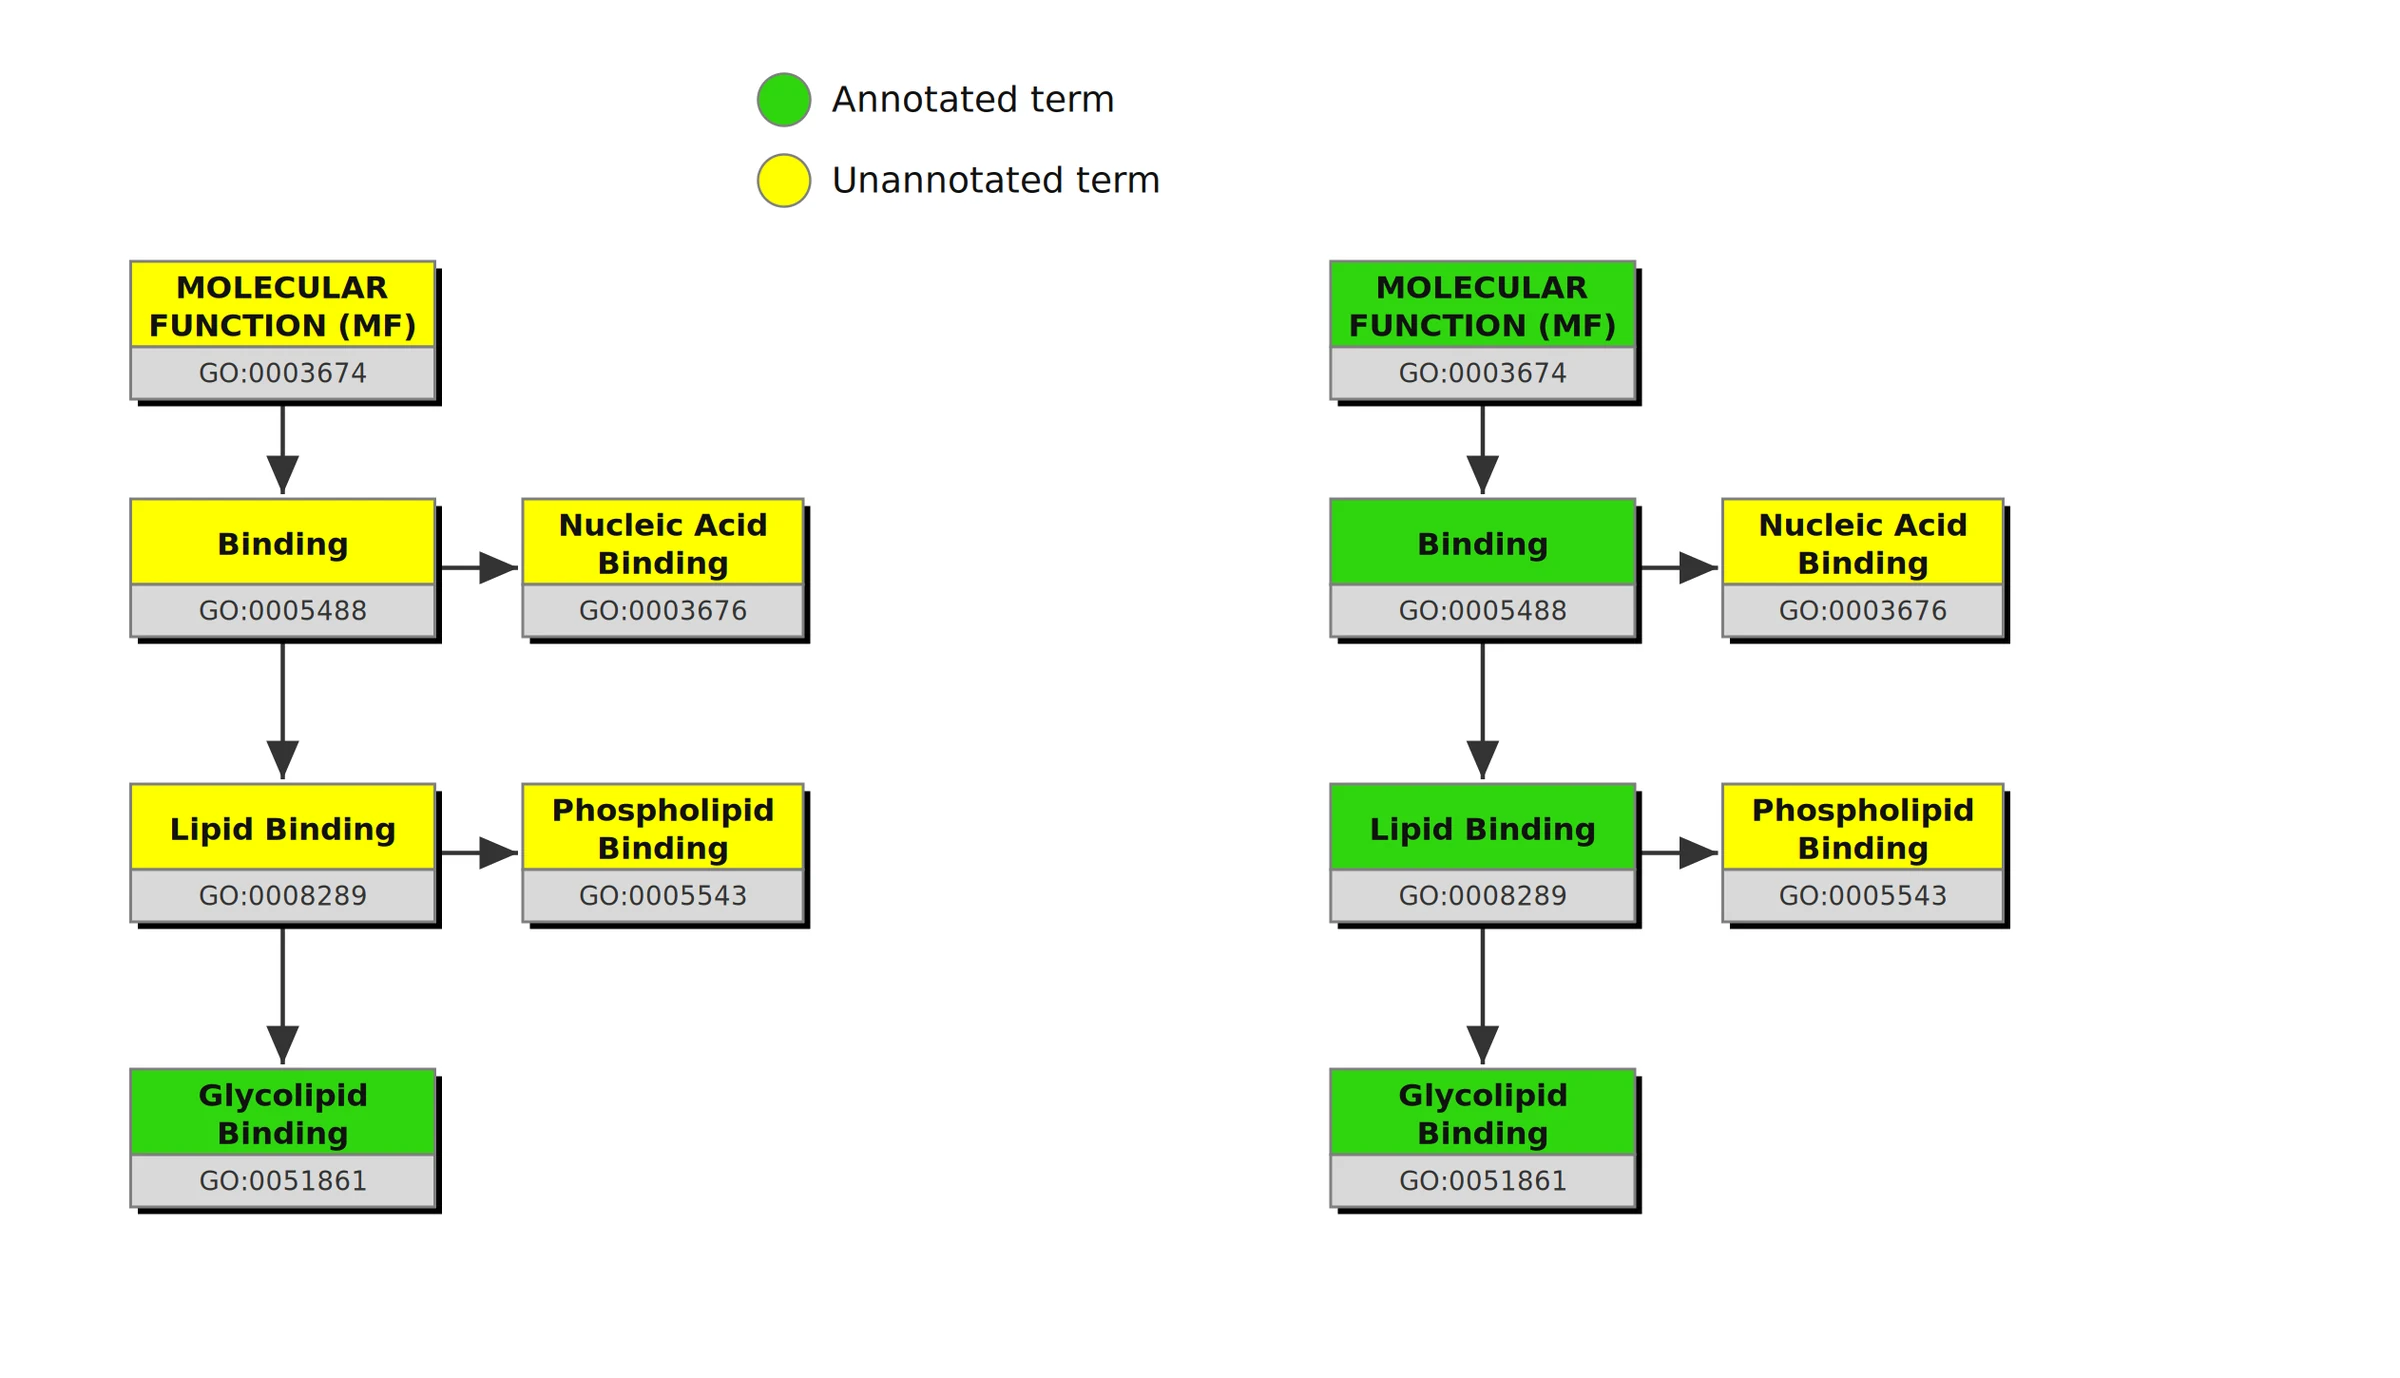
\includegraphics[width=775.3\px,height=445.2\px]{figures/fig_2_1.png}};
\fill<3>[plate] (1103.3,235) rectangle ++(387.7,445.2);
\node[tl] at (88,70) {\fmR\fz{16}{16}\color{inkii}\ls{2}\Ll{1 · Motivation}};
\node[tl] at (88,131) {\fdA\fz{54}{56.7}\color{ink}\ls{-1}\Ll{Function as a hierarchy of terms}};
\node<2-5>[tl] at (124,236) {\fbR\fz{30}{40.5}\color{ink}\Ll{Three ontologies: Biological Process\\(BP), Cellular Component (CC),\\Molecular Function (MF)}};
\node<3-5>[tl] at (124,379.5) {\fbR\fz{30}{40.5}\color{ink}\Ll{Each is a directed acyclic graph of terms\\({\fmR\fz{25.8}{31}{}is\_a}, {\fmR\fz{25.8}{31}{}part\_of})}};
\node<4-5>[tl] at (124,482.5) {\fbR\fz{30}{40.5}\color{ink}\Ll{True Path Rule: a term implies all\\its ancestors}};
\node<5>[tl] at (124,585.5) {\fbR\fz{30}{40.5}\color{ink}\Ll{Task: hierarchical multi-\\label classification}};
\node<3-5>[tl] at (694.7,718.2) {\fmR\fz{15}{19.5}\color{muted}\Ll{Dissertation, Fig. 2.1 · left inconsistent, right consistent}};
\node[tr] at (1512,876) {\fmR\fz{16}{16}\color{muted}4 / 45};
\end{tikzpicture}
\note{A protein carries many terms at different levels of specificity. If a specific term is annotated, every ancestor must be too. 

Predictions are made hierarchy-consistent before any metric is computed.}
\end{frame}

\begin{frame}[plain]
\begin{tikzpicture}[deck]
\node<1>[box] at (0,0) {\includegraphics[page=3,width=1600\px]{build/layers}};
\node<2>[box] at (0,0) {\includegraphics[page=11,width=1600\px]{build/layers}};
\node<3>[box] at (0,0) {\includegraphics[page=12,width=1600\px]{build/layers}};
\node<4>[box] at (0,0) {\includegraphics[page=13,width=1600\px]{build/layers}};
\node<2-4>[box] at (715.7,235) {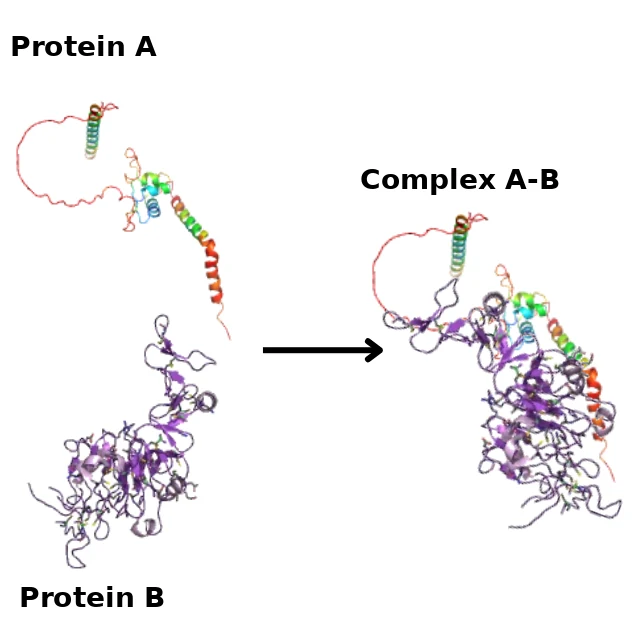
\includegraphics[width=223\px,height=223\px]{figures/fig_2_2.png}};
\node[tl] at (88,70) {\fmR\fz{16}{16}\color{inkii}\ls{2}\Ll{1 · Motivation}};
\node[tl] at (88,131) {\fdA\fz{54}{56.7}\color{ink}\ls{-1}\Ll{Function also depends on context}};
\node<2-4>[tl] at (124,236) {\fbR\fz{30}{40.5}\color{ink}\Ll{Proteins act in complexes and pathways}};
\node<2-4>[tl] at (124,298.5) {\fbR\fz{30}{40.5}\color{ink}\Ll{PPI networks: nodes are proteins, edges\\are associations}};
\node<3-4>[tl] at (124,401.5) {\fbR\fz{30}{40.5}\color{ink}\Ll{Guilt by association: connected proteins\\tend to share functions}};
\node<4>[tl] at (124,504.5) {\fbR\fz{30}{40.5}\color{ink}\Ll{But STRING mixes evidence of uneven\\reliability, and about one third of\\proteins have no edge}};
\node<2-4>[tl] at (694.7,496) {\fmR\fz{15}{19.5}\color{muted}\Ll{Dissertation, Fig. 2.2}};
\node[tr] at (1512,876) {\fmR\fz{16}{16}\color{muted}5 / 45};
\end{tikzpicture}
\note{Sequence-derived features are strong, but part of a protein's function is set by its cellular context. 

STRING aggregates experiments, curated databases, co-expression, genomic context and text mining into one confidence score. 

Coverage is uneven, which becomes the central limitation of a network-only model.}
\end{frame}

\begin{frame}[plain]
\begin{tikzpicture}[deck]
\node<1>[box] at (0,0) {\includegraphics[page=3,width=1600\px]{build/layers}};
\node<2>[box] at (0,0) {\includegraphics[page=14,width=1600\px]{build/layers}};
\node<3>[box] at (0,0) {\includegraphics[page=15,width=1600\px]{build/layers}};
\node<4>[box] at (0,0) {\includegraphics[page=16,width=1600\px]{build/layers}};
\node[tl] at (88,70) {\fmR\fz{16}{16}\color{inkii}\ls{2}\Ll{1 · Motivation}};
\node[tl] at (88,131) {\fdA\fz{54}{56.7}\color{ink}\ls{-1}\Ll{Seven research questions}};
\node<2-4>[tc] at (126,236) {\fmM\fz{20}{20}\color{ink}\Lc{RQ1}};
\node<2-4>[tl] at (184,236) {\fbR\fz{30}{39}\color{ink}\Ll{Which network representation works best?}};
\node<2-4>[tc] at (126,308) {\fmM\fz{20}{20}\color{ink}\Lc{RQ2}};
\node<2-4>[tl] at (184,308) {\fbR\fz{30}{39}\color{ink}\Ll{How much does propagating ProtT5 over\\STRING add?}};
\node<2-4>[tc] at (126,416) {\fmM\fz{20}{20}\color{ink}\Lc{RQ3}};
\node<2-4>[tl] at (184,416) {\fbR\fz{30}{39}\color{ink}\Ll{Fixed vs learned aggregation, vector vs\\image heads}};
\node<3-4>[tc] at (126,524) {\fmM\fz{20}{20}\color{ink}\Lc{RQ4}};
\node<3-4>[tl] at (184,524) {\fbR\fz{30}{39}\color{ink}\Ll{Do early and late fusion help?}};
\node<3-4>[tc] at (866,236) {\fmM\fz{20}{20}\color{ink}\Lc{RQ5}};
\node<3-4>[tl] at (924,236) {\fbR\fz{30}{39}\color{ink}\Ll{How deep, and how much retention?}};
\node<4>[tc] at (866,308) {\fmM\fz{20}{20}\color{ink}\Lc{RQ6}};
\node<4>[tl] at (924,308) {\fbR\fz{30}{39}\color{ink}\Ll{How does it compare with the literature?}};
\node<4>[tc] at (866,416) {\fmM\fz{20}{20}\color{ink}\Lc{RQ7}};
\node<4>[tl] at (924,416) {\fbR\fz{30}{39}\color{ink}\Ll{Does it work on one global, aggregated\\network?}};
\node[tr] at (1512,876) {\fmR\fz{16}{16}\color{muted}6 / 45};
\end{tikzpicture}
\note{Read the full questions from Section 1.3 only if asked. Each one is answered on the conclusions slide.}
\end{frame}

\begin{frame}[plain]
\begin{tikzpicture}[deck]
\node<1>[box] at (0,0) {\includegraphics[page=3,width=1600\px]{build/layers}};
\node<2>[box] at (0,0) {\includegraphics[page=17,width=1600\px]{build/layers}};
\node<3>[box] at (0,0) {\includegraphics[page=18,width=1600\px]{build/layers}};
\node<4>[box] at (0,0) {\includegraphics[page=19,width=1600\px]{build/layers}};
\node[tl] at (88,70) {\fmR\fz{16}{16}\color{inkii}\ls{2}\Ll{1 · Motivation}};
\node[tl] at (88,131) {\fdA\fz{54}{56.7}\color{ink}\ls{-1}\Ll{Contributions}};
\node<2-4>[tl] at (144,237) {\fbR\fz{32}{41.6}\color{ink}\Ll{NEXUS-GO: non-parametric multi-hop propagation of ProtT5 embeddings over STRING}};
\node<2-4>[tl] at (144,304.6) {\fbR\fz{32}{41.6}\color{ink}\Ll{Controlled comparison of fixed vs learned (GCN, GAT) aggregation}};
\node<2-4>[tl] at (144,372.2) {\fbR\fz{32}{41.6}\color{ink}\Ll{Vector vs image classification heads over the same embeddings}};
\node<3-4>[tl] at (144,439.8) {\fbR\fz{32}{41.6}\color{ink}\Ll{Early and late fusion of fixed and learned routes}};
\node<3-4>[tl] at (144,507.4) {\fbR\fz{32}{41.6}\color{ink}\Ll{Benchmark against five reimplemented methods, same splits and setting}};
\node<4>[tl] at (88,768.7) {\fmM\fz{18}{21.6}\color{ink}\Ll{VISAPP 2026 · published, pp. 157–166}};
\node<4>[tl] at (88,800.3) {\fbR\fz{21}{28.4}\color{inkii}\Ll{{\fbI\color{ink}{}From Graphs to Images: Non-Parametric PPI Context Integration for}\\{\fbI\color{ink}{}Vision-Based Protein Function Prediction}}};
\node<4>[tl] at (824,768.7) {\fmM\fz{18}{21.6}\color{ink}\Ll{CCIS · accepted, expected December 2026}};
\node<4>[tl] at (824,800.3) {\fbR\fz{21}{28.4}\color{inkii}\Ll{{\fbI\color{ink}{}Beyond Learnable Graphs: Fixed Multi-Hop PPI Diffusion of Sequence}\\{\fbI\color{ink}{}Embeddings for Robust Protein Function Prediction} · extended version}};
\node[tr] at (1512,876) {\fmR\fz{16}{16}\color{muted}7 / 45};
\end{tikzpicture}
\note{Five contributions, each answered with a result at the end. 

The first paper reported the first, sum-deduplicated campaign; the extended version continues the fixed route and adds a vector head next to the vision head. It was accepted in Communications in Computer and Information Science.}
\end{frame}

\section{2 · Background and related work}
\begin{frame}[plain]
\begin{tikzpicture}[deck]
\node<1>[box] at (0,0) {\includegraphics[page=3,width=1600\px]{build/layers}};
\node<2>[box] at (0,0) {\includegraphics[page=20,width=1600\px]{build/layers}};
\node<3>[box] at (0,0) {\includegraphics[page=21,width=1600\px]{build/layers}};
\node<4>[box] at (0,0) {\includegraphics[page=22,width=1600\px]{build/layers}};
\node<5>[box] at (0,0) {\includegraphics[page=23,width=1600\px]{build/layers}};
\node<2-5>[box] at (123.6,235) {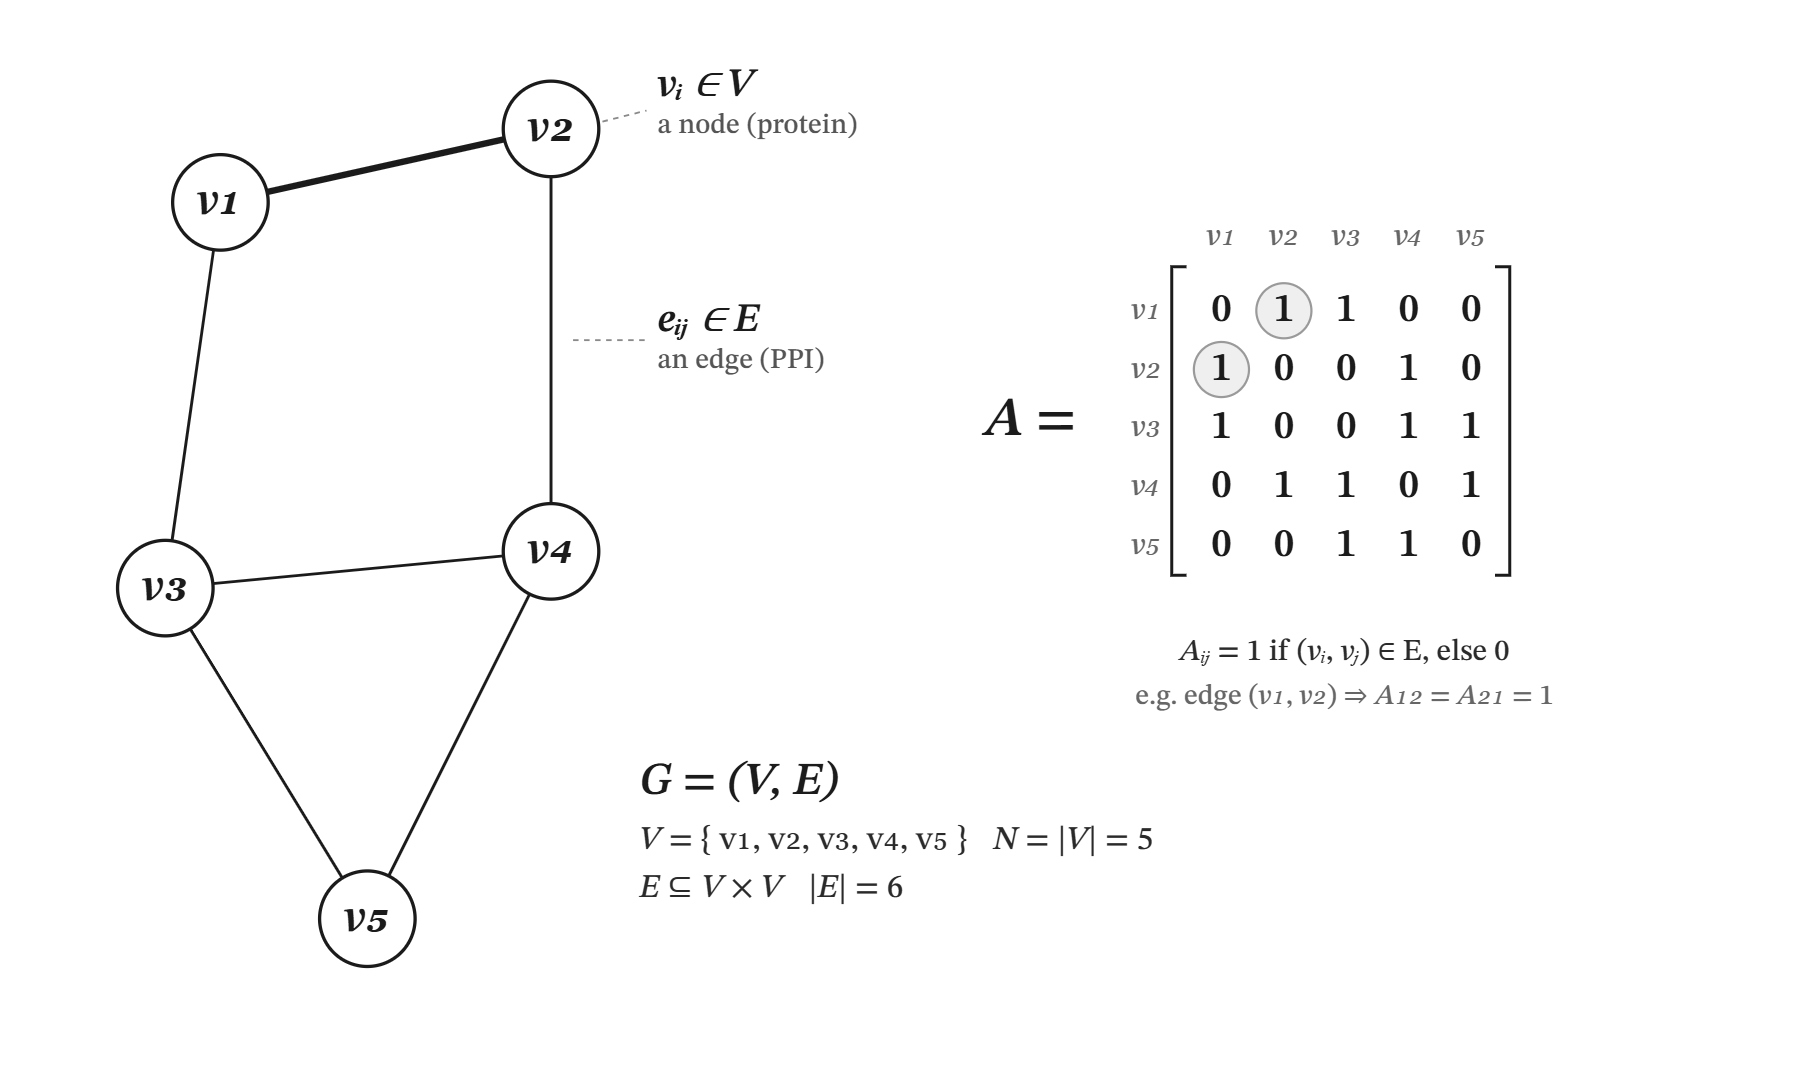
\includegraphics[width=624.8\px,height=370\px]{figures/fig_2_3.png}};
\node[tl] at (88,70) {\fmR\fz{16}{16}\color{inkii}\ls{2}\Ll{2 · Background and related work}};
\node[tl] at (88,131) {\fdA\fz{54}{56.7}\color{ink}\ls{-1}\Ll{Graphs, adjacency and message passing}};
\node<2-5>[tl] at (88,643) {\fmR\fz{15}{19.5}\color{muted}\Ll{Dissertation, Fig. 2.3}};
\node<2-5>[tl] at (124,689) {\fbR\fz{26}{35.1}\color{ink}\Ll{{\fz{29.2}{35}$G = (V, E, w)$}: proteins, associations,\\STRING confidence}};
\node<3-5>[tl] at (852,689) {\fbR\fz{26}{35.1}\color{ink}\Ll{Message passing: aggregate neighbours, update\\the node}};
\node<2-5>[tl] at (124,775.2) {\fbR\fz{26}{35.1}\color{ink}\Ll{Adjacency matrix {\fz{29.2}{35}$A$}; sparse storage {\fz{29.2}{35}$O(|E|)$}}};
\node<5>[tl] at (852,775.2) {\fbR\fz{26}{35.1}\color{ink}\Ll{{\fz{29.2}{35}$L$} layers reach {\fz{29.2}{35}$L$} hops; too many cause oversmoothing}};
\node[tr] at (1512,876) {\fmR\fz{16}{16}\color{muted}8 / 45};
\end{tikzpicture}
\note{GCN aggregates with a symmetrically normalized adjacency; GAT learns attention weights over neighbours. 

Each layer widens the receptive field by one hop, and too many layers make neighbouring representations indistinguishable.}
\end{frame}

\begin{frame}[plain]
\begin{tikzpicture}[deck]
\node<1>[box] at (0,0) {\includegraphics[page=3,width=1600\px]{build/layers}};
\node<2>[box] at (0,0) {\includegraphics[page=24,width=1600\px]{build/layers}};
\node<3>[box] at (0,0) {\includegraphics[page=25,width=1600\px]{build/layers}};
\node<4>[box] at (0,0) {\includegraphics[page=26,width=1600\px]{build/layers}};
\node<3-4>[box] at (594.3,440) {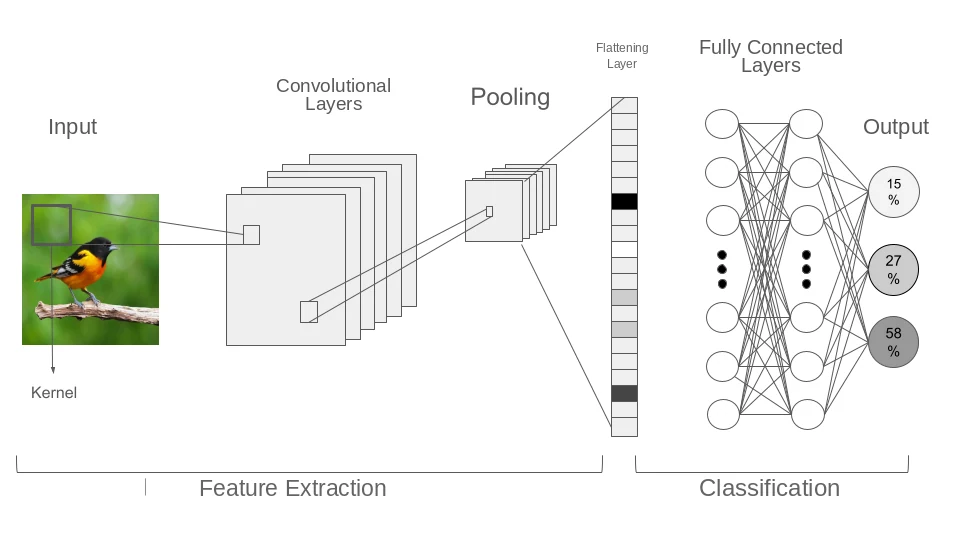
\includegraphics[width=411.3\px,height=231.4\px]{figures/fig_2_6.png}};
\node<4>[box] at (1079.7,435.7) {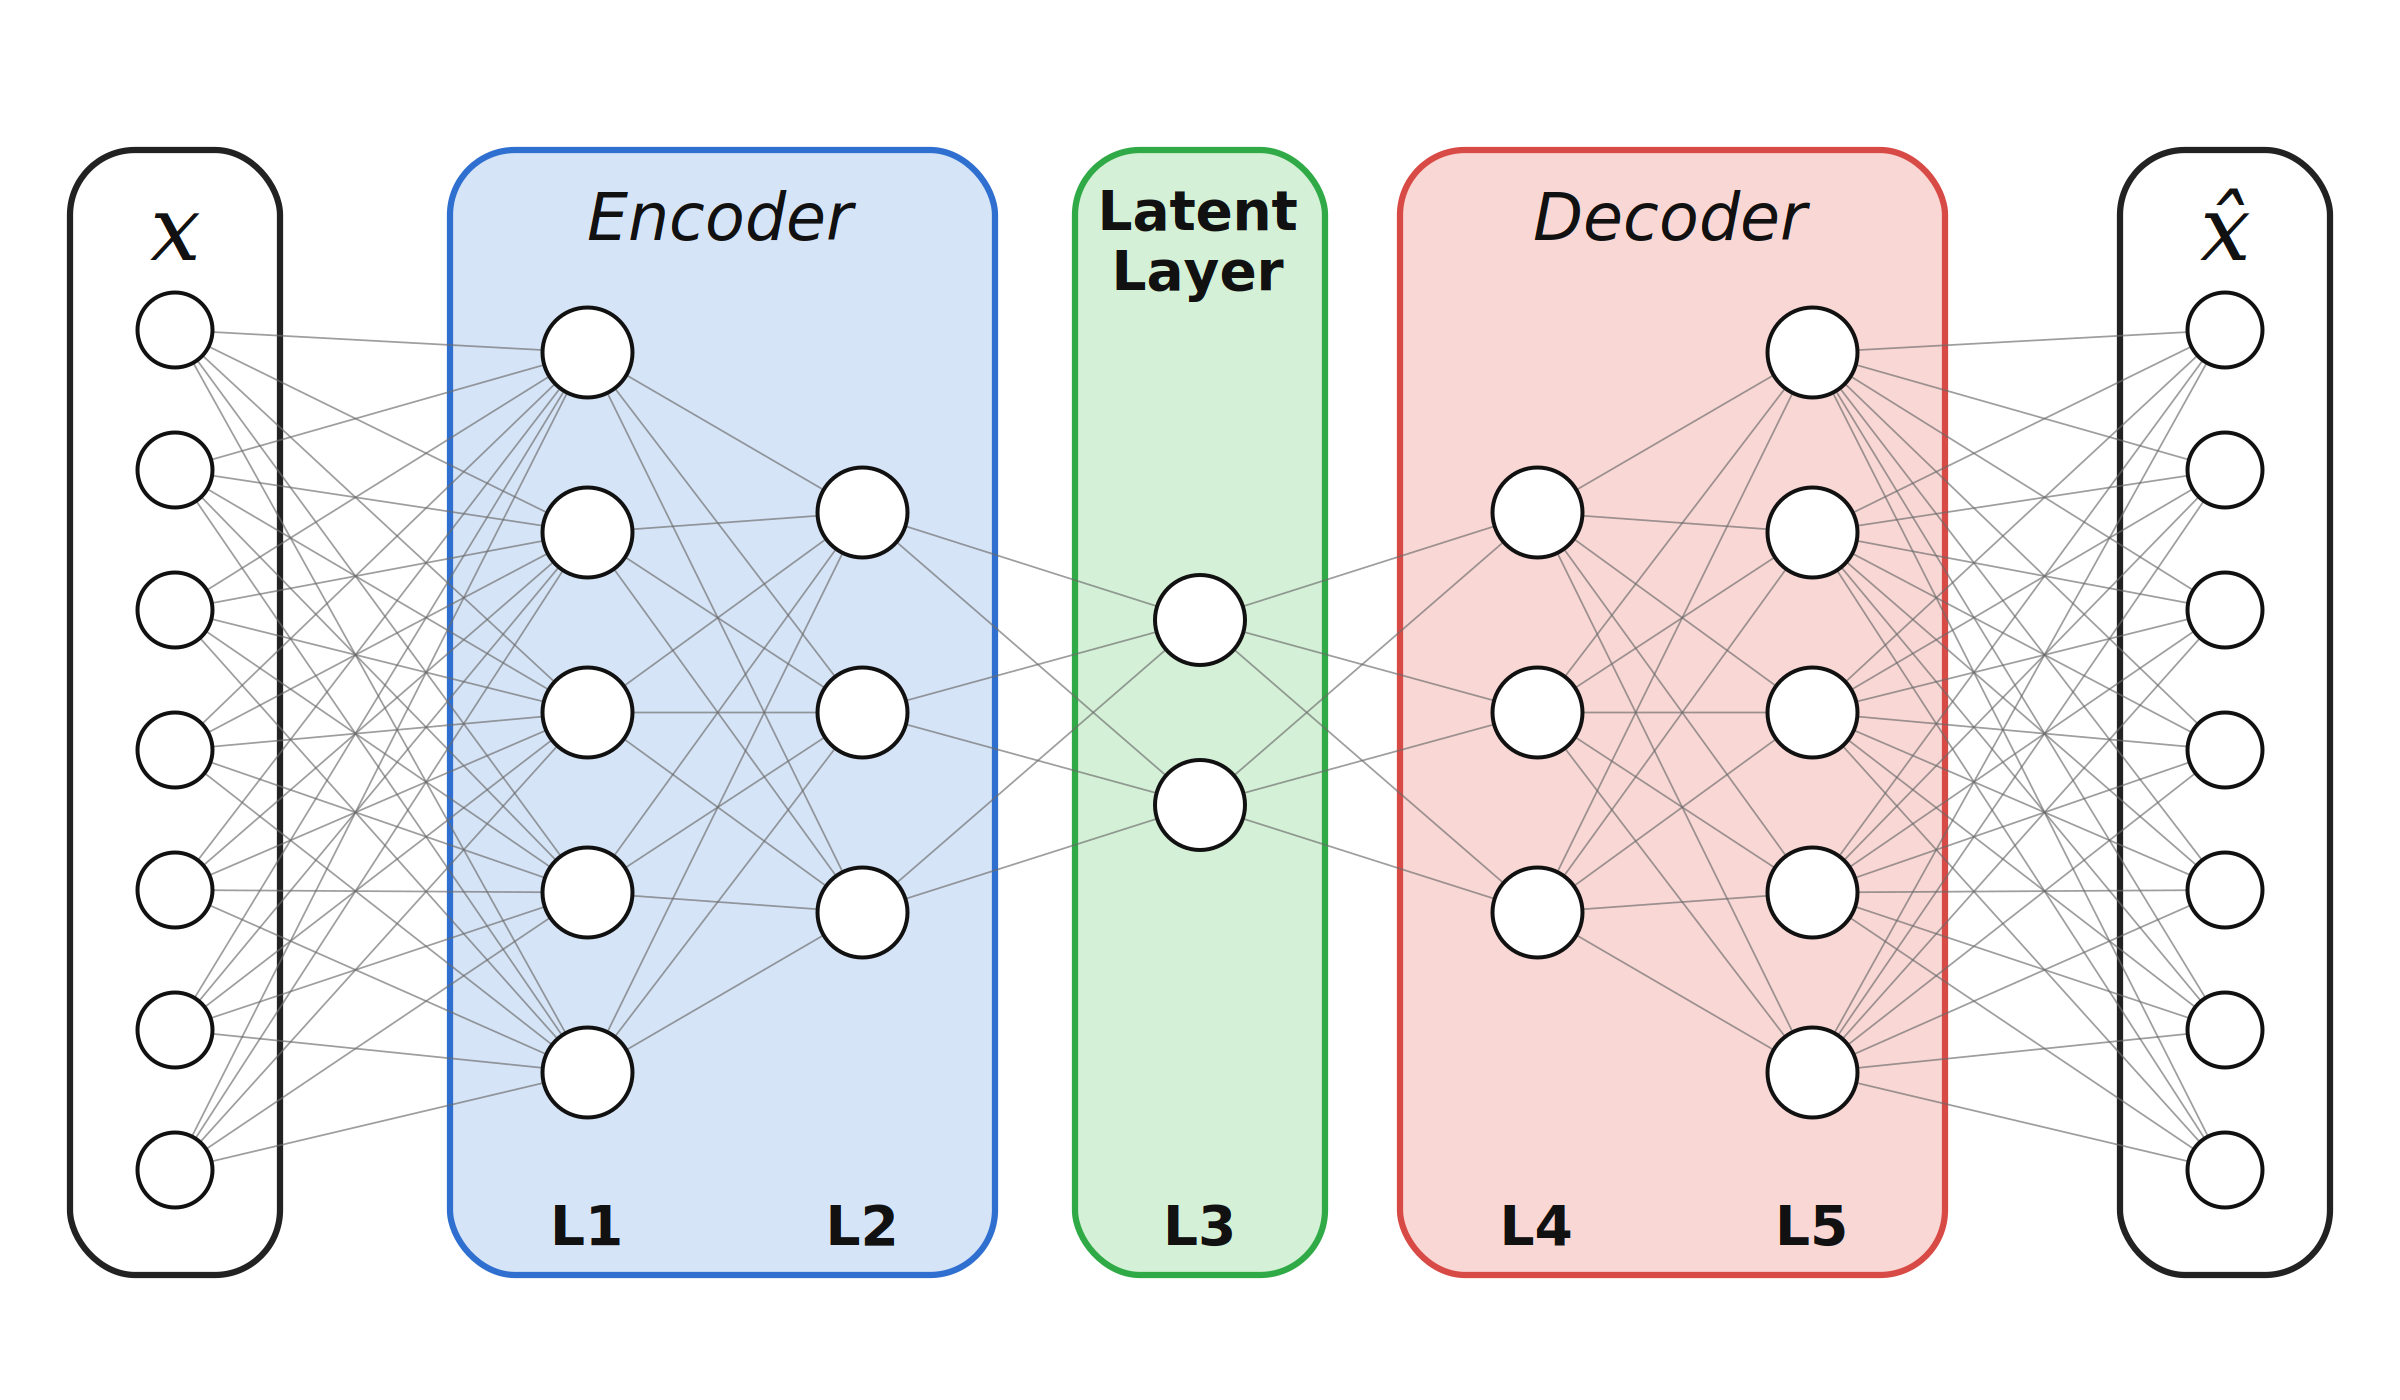
\includegraphics[width=411.3\px,height=239.9\px]{figures/fig_2_7.png}};
\node[tl] at (88,70) {\fmR\fz{16}{16}\color{inkii}\ls{2}\Ll{2 · Background and related work}};
\node[tl] at (88,131) {\fdA\fz{54}{56.7}\color{ink}\ls{-1}\Ll{Building blocks}};
\node<2-4>[tl] at (88,230) {\fbR\fz{24}{32.4}\color{ink}\Ll{{\fbB{}MLP}: the vector prediction head}};
\node<3-4>[tl] at (573.3,230) {\fbR\fz{24}{32.4}\color{ink}\Ll{{\fbB{}CNN}: the backbone of the image route\\(ResNet-50, ConvNeXt-Tiny)}};
\node<4>[tl] at (1058.7,230) {\fbR\fz{24}{32.4}\color{ink}\Ll{{\fbB{}Autoencoder}: the compression inside\\deepNF, one of the baselines}};
\node<2-4>[tl] at (88,854.9) {\fmR\fz{15}{19.5}\color{muted}\Ll{Dissertation, Figs. 2.4 and 2.5}};
\node<3-4>[tl] at (573.3,831.5) {\fmR\fz{15}{19.5}\color{muted}\Ll{Dissertation, Fig. 2.6}};
\node<4>[tl] at (1058.7,831.5) {\fmR\fz{15}{19.5}\color{muted}\Ll{Dissertation, Fig. 2.7}};
\node[tr] at (1512,876) {\fmR\fz{16}{16}\color{muted}9 / 45};
\end{tikzpicture}
\note{Only what the rest of the talk needs. 

The MLP is the vector head, the CNN is the vision head, and the autoencoder is how deepNF compresses diffusion states.}
\end{frame}

\begin{frame}[plain]
\begin{tikzpicture}[deck]
\node<1>[box] at (0,0) {\includegraphics[page=3,width=1600\px]{build/layers}};
\node<2>[box] at (0,0) {\includegraphics[page=27,width=1600\px]{build/layers}};
\node<3>[box] at (0,0) {\includegraphics[page=28,width=1600\px]{build/layers}};
\node<4>[box] at (0,0) {\includegraphics[page=29,width=1600\px]{build/layers}};
\node<5>[box] at (0,0) {\includegraphics[page=30,width=1600\px]{build/layers}};
\node[tl] at (88,70) {\fmR\fz{16}{16}\color{inkii}\ls{2}\Ll{2 · Background and related work}};
\node[tl] at (88,131) {\fdA\fz{54}{56.7}\color{ink}\ls{-1}\Ll{Protein language models}};
\node<2-5>[tl] at (124,236) {\fbR\fz{30}{40.5}\color{ink}\Ll{Self-supervised pretraining on hundreds\\of millions of sequences}};
\node<3-5>[tl] at (124,339) {\fbR\fz{30}{40.5}\color{ink}\Ll{Transformer encoder: every residue\\attends to every other}};
\node<4-5>[tl] at (124,442) {\fbR\fz{30}{40.5}\color{ink}\Ll{ProtT5-XL-U50: T5 encoder, BFD then\\UniRef50, 15\% residue masking}};
\node<5>[tl] at (124,545) {\fbR\fz{30}{40.5}\color{ink}\Ll{Used here as a frozen feature extractor}};
\node[tr] at (1512,876) {\fmR\fz{16}{16}\color{muted}10 / 45};
\end{tikzpicture}
\note{Language models turn function prediction into ordinary multi-label classification over a fixed-length vector. 

No gradient from our task reaches ProtT5; we read three encoder layers and keep them fixed.}
\end{frame}

\begin{frame}[plain]
\begin{tikzpicture}[deck]
\node<1>[box] at (0,0) {\includegraphics[page=3,width=1600\px]{build/layers}};
\node<2>[box] at (0,0) {\includegraphics[page=31,width=1600\px]{build/layers}};
\node<3>[box] at (0,0) {\includegraphics[page=32,width=1600\px]{build/layers}};
\node<4>[box] at (0,0) {\includegraphics[page=33,width=1600\px]{build/layers}};
\node[tl] at (88,70) {\fmR\fz{16}{16}\color{inkii}\ls{2}\Ll{2 · Background and related work}};
\node[tl] at (88,131) {\fdA\fz{54}{56.7}\color{ink}\ls{-1}\Ll{From neighbour voting to graph transformers}};
\node[tr] at (1512,876) {\fmR\fz{16}{16}\color{muted}11 / 45};
\end{tikzpicture}
\note{The field moved from fixed diffusion to learned attention, and each step added parameters. 

Decoupled methods such as SGC and APPNP move against that trend, and SEGT-GO's multi-hop aggregation is itself a plain matrix product.}
\end{frame}

\begin{frame}[plain]
\begin{tikzpicture}[deck]
\node<1-2>[box] at (0,0) {\includegraphics[page=3,width=1600\px]{build/layers}};
\node<3>[box] at (0,0) {\includegraphics[page=34,width=1600\px]{build/layers}};
\node<4>[box] at (0,0) {\includegraphics[page=35,width=1600\px]{build/layers}};
\node<5>[box] at (0,0) {\includegraphics[page=36,width=1600\px]{build/layers}};
\node[tl] at (88,70) {\fmR\fz{16}{16}\color{inkii}\ls{2}\Ll{2 · Background and related work}};
\node[tl] at (88,131) {\fdA\fz{54}{56.7}\color{ink}\ls{-1}\Ll{The open question}};
\node<2-5>[tl] at (88,262) {\fdA\fz{64}{69.1}\color{ink}\ls{-1.5}\Ll{Is a learned graph component still needed\\once the propagated object is informative?}};
\node<3-5>[tl] at (124,426.2) {\fbR\fz{30}{40.5}\color{ink}\Ll{Proposal: propagate ProtT5 embeddings with a fixed, finite-step operator, then use an\\ordinary head}};
\node<4-5>[tl] at (124,529.2) {\fbR\fz{30}{40.5}\color{ink}\Ll{A sequence representation exists for every protein, so the network adds instead\\of supplies}};
\node<5>[tl] at (124,632.2) {\fbR\fz{30}{40.5}\color{ink}\Ll{No prior visual route starts from a propagated language-model embedding}};
\node[tr] at (1512,876) {\fmR\fz{16}{16}\color{muted}12 / 45};
\end{tikzpicture}
\note{The contribution is an architectural placement, not a new propagation mechanism. 

To our knowledge no previous work propagates protein language model embeddings directly while simplifying what consumes them.}
\end{frame}

\section{3 · Data and evaluation}
\begin{frame}[plain]
\begin{tikzpicture}[deck]
\node<1>[box] at (0,0) {\includegraphics[page=3,width=1600\px]{build/layers}};
\node<2>[box] at (0,0) {\includegraphics[page=37,width=1600\px]{build/layers}};
\node<3>[box] at (0,0) {\includegraphics[page=38,width=1600\px]{build/layers}};
\node<4>[box] at (0,0) {\includegraphics[page=39,width=1600\px]{build/layers}};
\node[tl] at (88,70) {\fmR\fz{16}{16}\color{inkii}\ls{2}\Ll{3 · Data and evaluation}};
\node[tl] at (88,131) {\fdA\fz{54}{56.7}\color{ink}\ls{-1}\Ll{Data: a CAFA5-derived corpus}};
\node<2-4>[tl] at (106,237) {\fbB\fz{20}{24}\color{inkii}\Ll{Ontology}};
\node<2-4>[tr] at (547.6,237) {\fbB\fz{20}{24}\color{inkii}\Lr{Training}};
\node<2-4>[tr] at (677.8,237) {\fbB\fz{20}{24}\color{inkii}\Lr{Validation}};
\node<2-4>[tr] at (797.8,237) {\fbB\fz{20}{24}\color{inkii}\Lr{Test}};
\node<2-4>[tr] at (891.1,237) {\fbB\fz{20}{24}\color{inkii}\Lr{Terms}};
\node<2-4>[tl] at (106,295) {\fbR\fz{28}{33.6}\color{ink}\Ll{Biological Process (BP)}};
\node<2-4>[tr] at (547.6,296) {\fmR\fz{28}{33.6}\color{ink}\Lr{73,768}};
\node<2-4>[tr] at (677.8,296) {\fmR\fz{28}{33.6}\color{ink}\Lr{9,221}};
\node<2-4>[tr] at (797.8,296) {\fmR\fz{28}{33.6}\color{ink}\Lr{9,221}};
\node<2-4>[tr] at (891.1,296) {\fmR\fz{28}{33.6}\color{ink}\Lr{500}};
\node<2-4>[tl] at (106,357) {\fbR\fz{28}{33.6}\color{ink}\Ll{Cellular Component (CC)}};
\node<2-4>[tr] at (547.6,358) {\fmR\fz{28}{33.6}\color{ink}\Lr{74,328}};
\node<2-4>[tr] at (677.8,358) {\fmR\fz{28}{33.6}\color{ink}\Lr{9,292}};
\node<2-4>[tr] at (797.8,358) {\fmR\fz{28}{33.6}\color{ink}\Lr{9,292}};
\node<2-4>[tr] at (891.1,358) {\fmR\fz{28}{33.6}\color{ink}\Lr{498}};
\node<2-4>[tl] at (106,419) {\fbR\fz{28}{33.6}\color{ink}\Ll{Molecular Function (MF)}};
\node<2-4>[tr] at (547.6,420) {\fmR\fz{28}{33.6}\color{ink}\Lr{62,909}};
\node<2-4>[tr] at (677.8,420) {\fmR\fz{28}{33.6}\color{ink}\Lr{7,864}};
\node<2-4>[tr] at (797.8,420) {\fmR\fz{28}{33.6}\color{ink}\Lr{7,864}};
\node<2-4>[tr] at (891.1,420) {\fmR\fz{28}{33.6}\color{ink}\Lr{499}};
\node<2-4>[tl] at (88,466) {\fmR\fz{15}{19.5}\color{muted}\Ll{Dissertation, Table 4.1}};
\node<3-4>[tl] at (973.3,236) {\fbR\fz{30}{40.5}\color{ink}\Ll{80 / 10 / 10 split, disjoint at\\protein level, no temporal or\\homology constraint}};
\node<4>[tl] at (973.3,379.5) {\fbR\fz{30}{40.5}\color{ink}\Ll{Labels per protein (mean): 25.91 BP,\\12.48 CC, 7.55 MF}};
\node<4>[tl] at (973.3,482.5) {\fbR\fz{30}{40.5}\color{ink}\Ll{Label matrix density:}};
\node<4>[tl] at (973.3,526) {\fmR\fz{22}{29.7}\color{inkii}\Ll{BP}};
\node<4>[tl] at (1164,526) {\fmR\fz{22}{29.7}\color{ink}\Ll{5.18\%}};
\node<4>[tl] at (973.3,565.7) {\fmR\fz{22}{29.7}\color{inkii}\Ll{CC}};
\node<4>[tl] at (1094.6,565.7) {\fmR\fz{22}{29.7}\color{ink}\Ll{2.51\%}};
\node<4>[tl] at (973.3,605.4) {\fmR\fz{22}{29.7}\color{inkii}\Ll{MF}};
\node<4>[tl] at (1068.6,605.4) {\fmR\fz{22}{29.7}\color{ink}\Ll{1.51\%}};
\node[tr] at (1512,876) {\fmR\fz{16}{16}\color{muted}13 / 45};
\end{tikzpicture}
\note{The official CAFA5 test labels were not available, so the splits come from the training corpus. 

Only about five hundred most frequent terms per ontology are kept, which makes absolute values not comparable with CAFA numbers.}
\end{frame}

\begin{frame}[plain]
\begin{tikzpicture}[deck]
\node<1>[box] at (0,0) {\includegraphics[page=3,width=1600\px]{build/layers}};
\node<2>[box] at (0,0) {\includegraphics[page=40,width=1600\px]{build/layers}};
\node<3>[box] at (0,0) {\includegraphics[page=41,width=1600\px]{build/layers}};
\node<4>[box] at (0,0) {\includegraphics[page=42,width=1600\px]{build/layers}};
\node<2-4>[box] at (109,235) {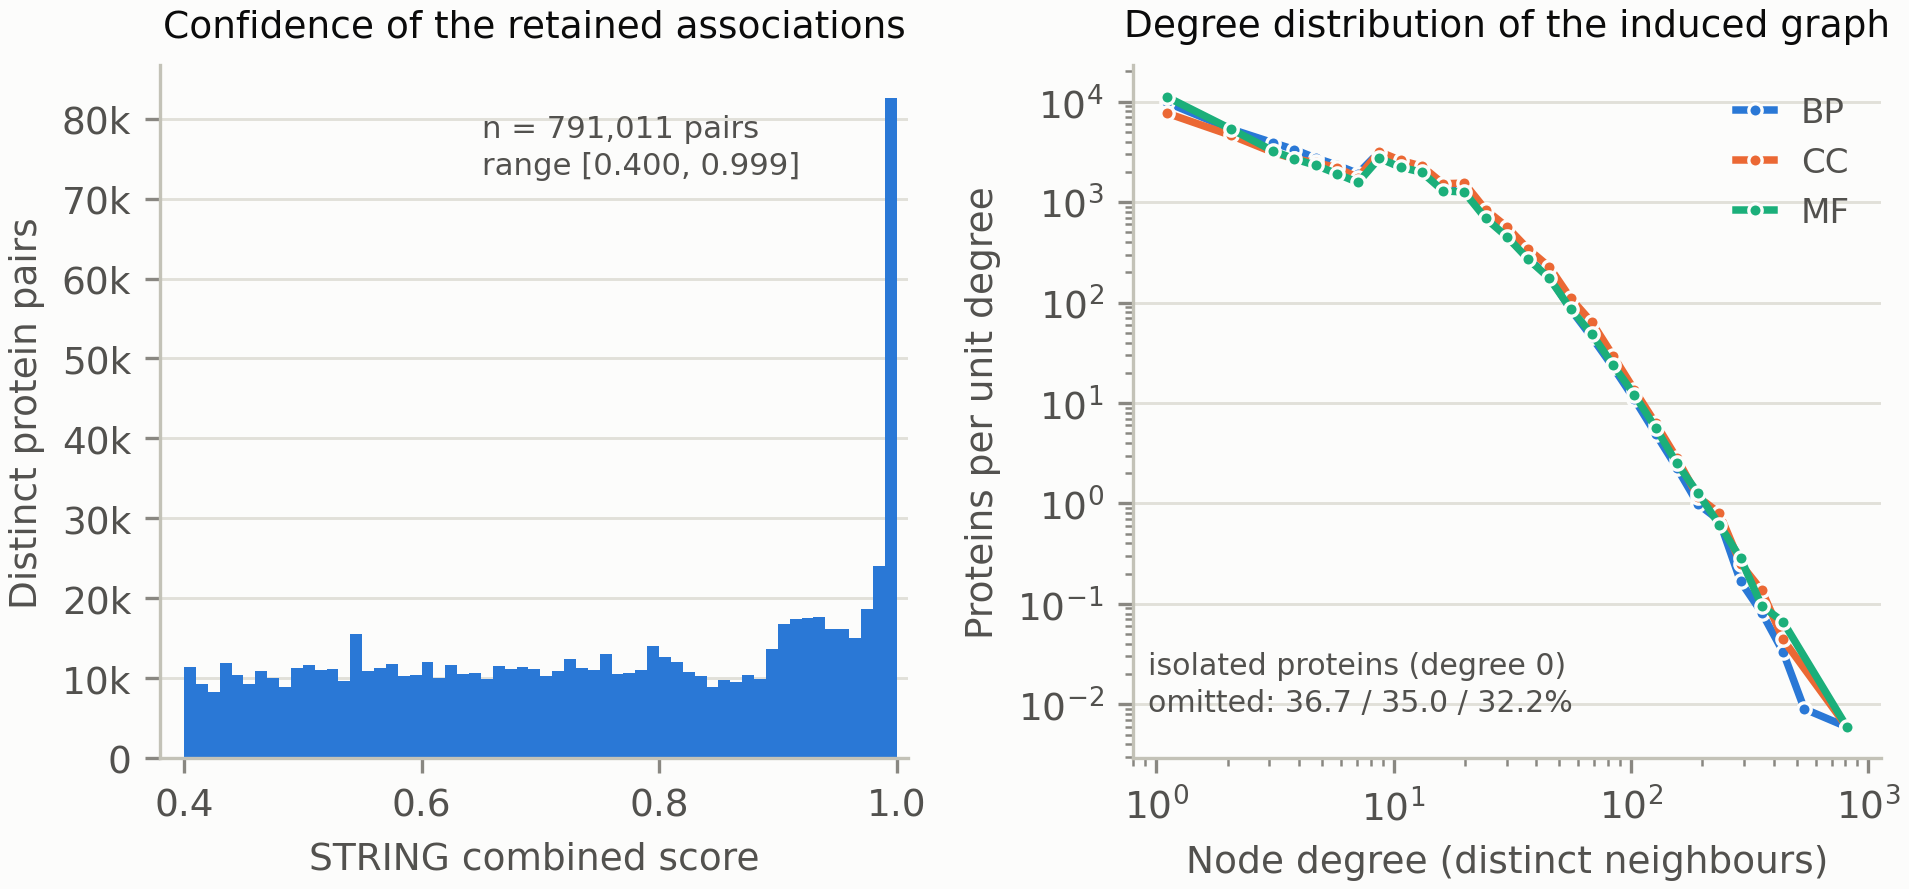
\includegraphics[width=775.3\px,height=361\px]{figures/fig_4_1.png}};
\fill<2-3>[plate] (496.7,235) rectangle ++(387.7,361);
\node[tl] at (88,70) {\fmR\fz{16}{16}\color{inkii}\ls{2}\Ll{3 · Data and evaluation}};
\node[tl] at (88,131) {\fdA\fz{54}{56.7}\color{ink}\ls{-1}\Ll{STRING v11.5: one aggregated network}};
\node<2-4>[tl] at (88,634) {\fmR\fz{15}{19.5}\color{muted}\Ll{Dissertation, Fig. 4.1 · left combined score, right degree}};
\node<2-4>[tl] at (973.3,232) {\fbR\fz{26}{35.1}\color{ink}\Ll{2,422,234 records, 791,011 distinct pairs,\\86,423 proteins}};
\node<2-4>[tl] at (973.3,318.2) {\fbR\fz{26}{35.1}\color{ink}\Ll{Combined score in [0.400, 0.999]; confidence,\\not binding strength}};
\node<3-4>[tl] at (973.3,404.4) {\fbR\fz{26}{35.1}\color{ink}\Ll{Each pair repeated 3.06 times on average (up\\to 170), always with the same score}};
\node<4>[tl] at (973.3,490.6) {\fbR\fz{26}{35.1}\color{ink}\Ll{Degree is heavy-tailed: median 5 to 7,\\maximum 763 to 805}};
\node[tr] at (1512,876) {\fmR\fz{16}{16}\color{muted}14 / 45};
\end{tikzpicture}
\note{The medium-confidence floor of 400 comes with the inherited file. 

Repeated records carry no extra score information, which later decides the deduplication rule. Some knowledge circularity with the annotations cannot be excluded.}
\end{frame}

\begin{frame}[plain]
\begin{tikzpicture}[deck]
\node<1>[box] at (0,0) {\includegraphics[page=3,width=1600\px]{build/layers}};
\node<2>[box] at (0,0) {\includegraphics[page=43,width=1600\px]{build/layers}};
\node<3>[box] at (0,0) {\includegraphics[page=44,width=1600\px]{build/layers}};
\node<2-3>[box] at (109,235.6) {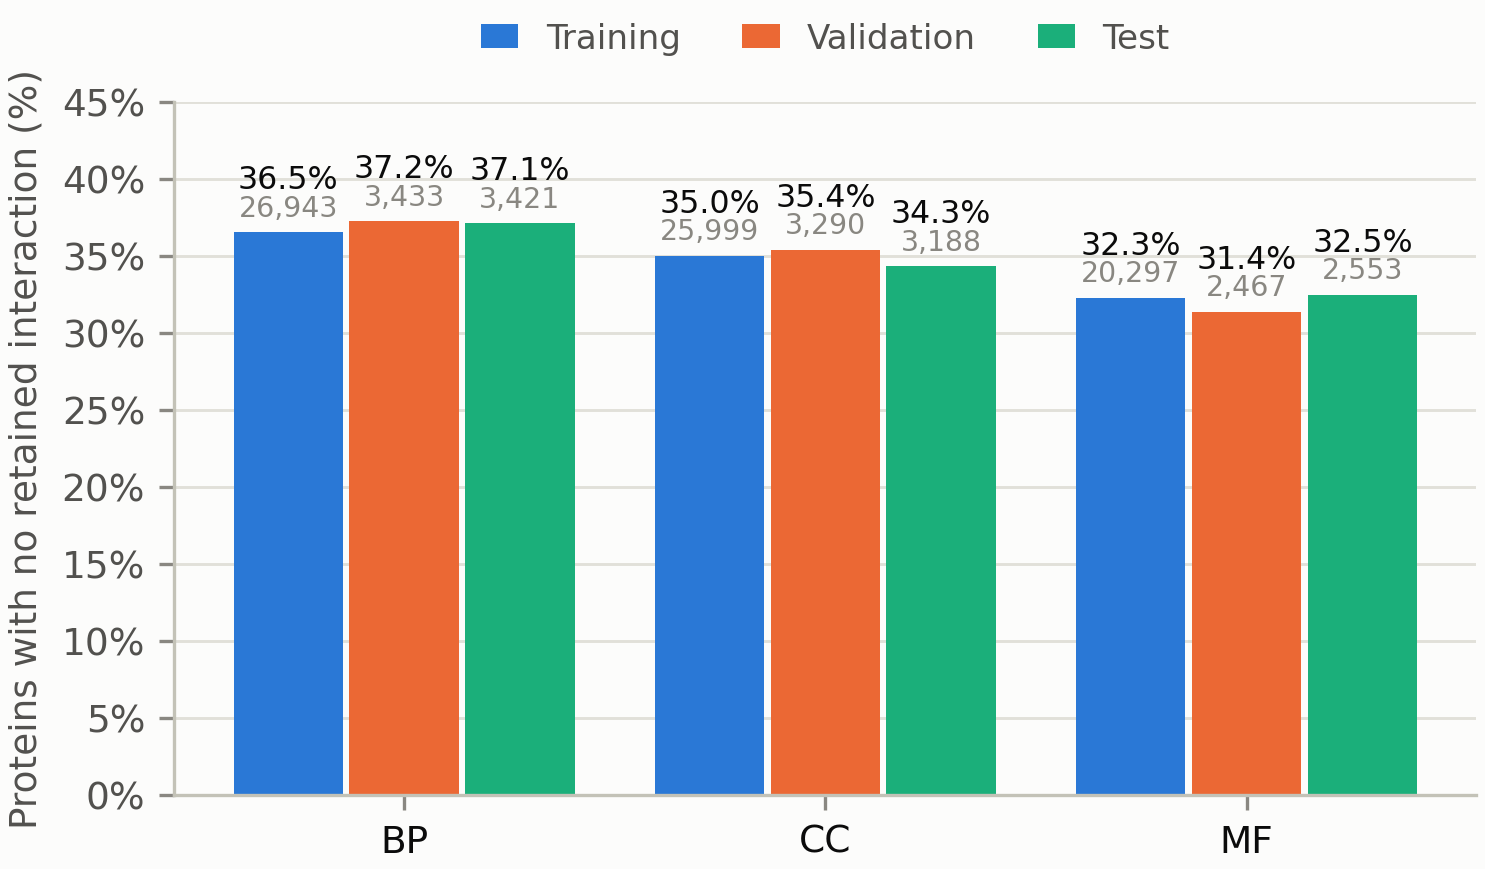
\includegraphics[width=654\px,height=382.7\px]{figures/fig_4_2.png}};
\node<3>[box] at (843.3,235) {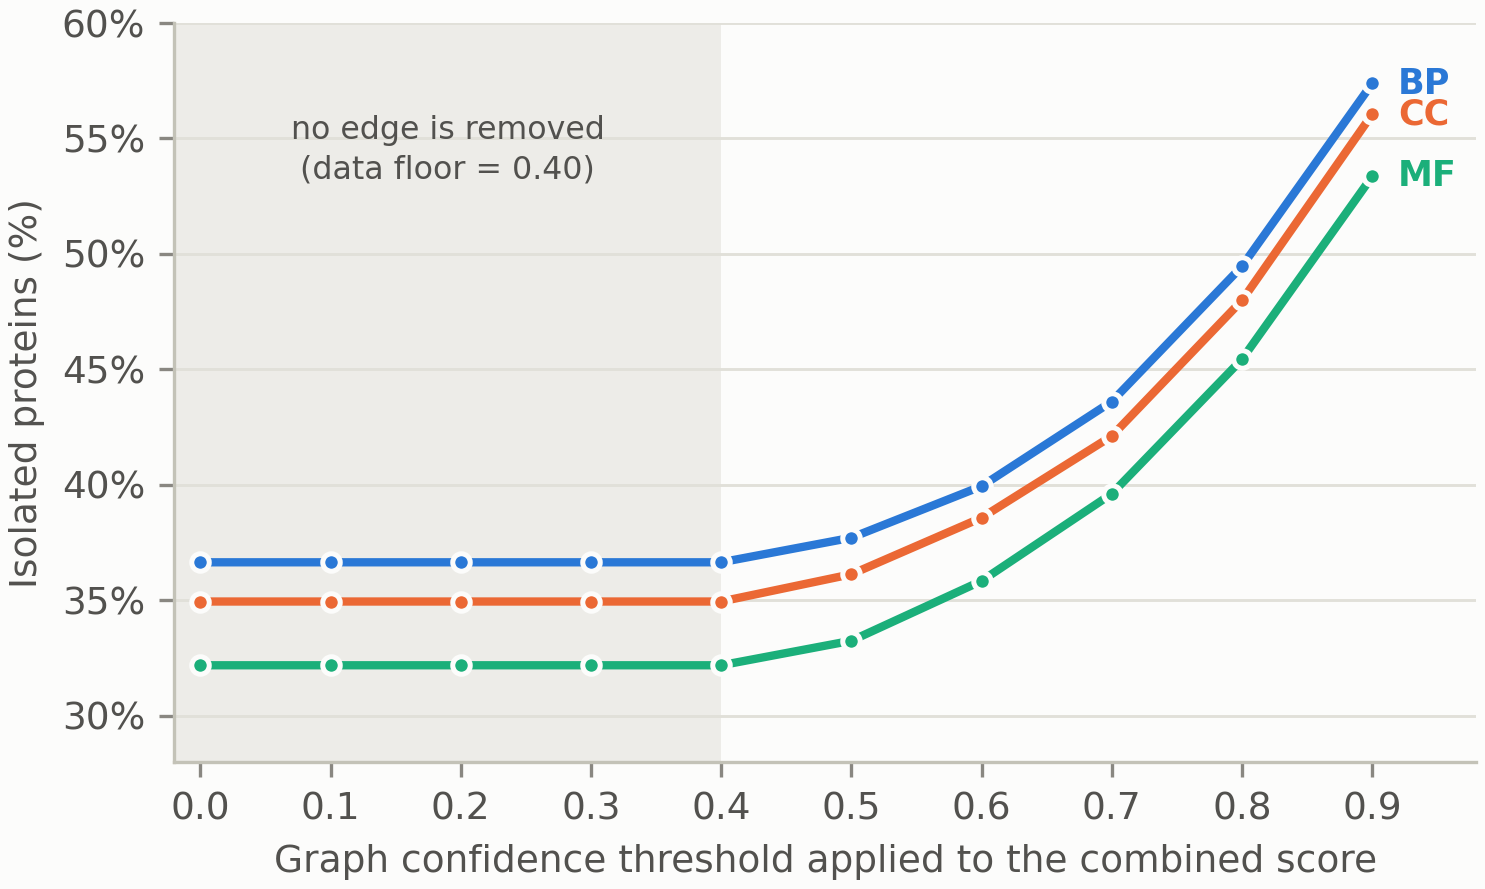
\includegraphics[width=641.4\px,height=384\px]{figures/fig_4_3.png}};
\node[tl] at (88,70) {\fmR\fz{16}{16}\color{inkii}\ls{2}\Ll{3 · Data and evaluation}};
\node[tl] at (88,131) {\fdA\fz{54}{56.7}\color{ink}\ls{-1}\Ll{One third of the proteins have no edge}};
\node<2-3>[tl] at (88,657) {\fmR\fz{15}{19.5}\color{muted}\Ll{Dissertation, Fig. 4.2}};
\node<2-3>[tl] at (124,719.5) {\fbR\fz{30}{40.5}\color{ink}\Ll{Isolated: 36.65\% BP, 34.95\% CC, 32.19\% MF}};
\node<2-3>[tl] at (124,782) {\fbR\fz{30}{40.5}\color{ink}\Ll{Stable across training, validation and test}};
\node<3>[tl] at (816,657) {\fmR\fz{15}{19.5}\color{muted}\Ll{Dissertation, Fig. 4.3}};
\node<3>[tl] at (852,719.5) {\fbR\fz{30}{40.5}\color{ink}\Ll{Thresholds up to 0.40 are inert; at 0.90 more\\than half the proteins are isolated}};
\node[tr] at (1512,876) {\fmR\fz{16}{16}\color{muted}15 / 45};
\end{tikzpicture}
\note{Isolated proteins were kept as nodes so that every protein is scored. For a model that sees only the network, these proteins have no input at all. 

This is the limitation the second generation is built to remove.}
\end{frame}

\begin{frame}[plain]
\begin{tikzpicture}[deck]
\node<1>[box] at (0,0) {\includegraphics[page=3,width=1600\px]{build/layers}};
\node<2>[box] at (0,0) {\includegraphics[page=7,width=1600\px]{build/layers}};
\node<3>[box] at (0,0) {\includegraphics[page=45,width=1600\px]{build/layers}};
\node<4>[box] at (0,0) {\includegraphics[page=46,width=1600\px]{build/layers}};
\node[tl] at (88,70) {\fmR\fz{16}{16}\color{inkii}\ls{2}\Ll{3 · Data and evaluation}};
\node[tl] at (88,131) {\fdA\fz{54}{56.7}\color{ink}\ls{-1}\Ll{Six protein-centric metrics}};
\node<2-4>[tl] at (124,236) {\fbR\fz{30}{40.5}\color{ink}\Ll{Primary criterion: wF\textsubscript{max}, information-\\content weighted}};
\node<3-4>[tl] at (124,339) {\fbR\fz{30}{40.5}\color{ink}\Ll{Also F\textsubscript{max}, F*\textsubscript{max} (root excluded), S\textsubscript{min}\\(bits, lower is better), AuPRC, IAuPRC}};
\node<4>[tl] at (124,442) {\fbR\fz{30}{40.5}\color{ink}\Ll{Predictions made hierarchy-consistent\\before scoring}};
\node<4>[tl] at (124,545) {\fbR\fz{30}{40.5}\color{ink}\Ll{101 thresholds; full evaluation mode\\(unpredicted proteins count as\\zero recall)}};
\node<2-4>[tl] at (694.7,261.7) {\fbR\fz{34}{40.8}\color{ink}\Ll{{\fz{38.2}{45.8}$\displaystyle wF_{\max} = \max_{\tau}\, \frac{2 \cdot wpr(\tau) \cdot wrc(\tau)}{wpr(\tau) + wrc(\tau)}$}}};
\node<2-4>[tl] at (694.7,341.4) {\fbR\fz{24}{32.4}\color{inkii}\Ll{each term weighted by its information content, {\fz{26.9}{32.3}$\mathrm{IC}(v) = -\log_2 \widehat{P}\bigl(v \mid \mathrm{pa}(v)\bigr)$}}};
\node<4>[tl] at (694.7,409.5) {\fbR\fz{34}{40.8}\color{ink}\Ll{{\fz{38.2}{45.8}$\displaystyle \tilde{s}_{iv} = \max_{u \in \mathcal{D}(v)} s_{iu}$}}};
\node[tr] at (1512,876) {\fmR\fz{16}{16}\color{muted}16 / 45};
\end{tikzpicture}
\note{wF\textsubscript{max} weights each term by information content, so frequent terms near the root count little. It is the selection criterion everywhere. 

The ancestor closure of predictions uses \texttt{is\_a} only, which matters most for CC.}
\end{frame}

\begin{frame}[plain]
\begin{tikzpicture}[deck]
\node<1>[box] at (0,0) {\includegraphics[page=3,width=1600\px]{build/layers}};
\node<2>[box] at (0,0) {\includegraphics[page=47,width=1600\px]{build/layers}};
\node<3>[box] at (0,0) {\includegraphics[page=48,width=1600\px]{build/layers}};
\node<4>[box] at (0,0) {\includegraphics[page=49,width=1600\px]{build/layers}};
\node<2-4>[box] at (109,235) {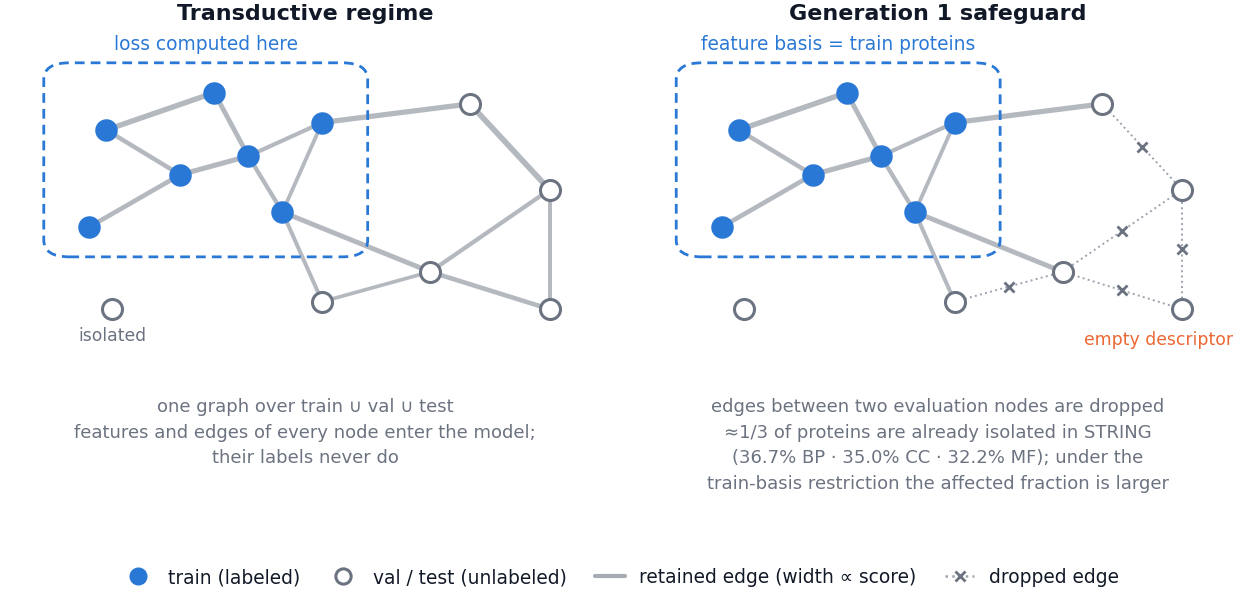
\includegraphics[width=775.3\px,height=373.3\px]{figures/fig_5_2.png}};
\node[tl] at (88,70) {\fmR\fz{16}{16}\color{inkii}\ls{2}\Ll{3 · Data and evaluation}};
\node[tl] at (88,131) {\fdA\fz{54}{56.7}\color{ink}\ls{-1}\Ll{Learning regime and protocol}};
\node<2-4>[tl] at (88,646.3) {\fmR\fz{15}{19.5}\color{muted}\Ll{Dissertation, Fig. 5.2}};
\node<2-4>[tl] at (973.3,232) {\fbR\fz{26}{35.1}\color{ink}\Ll{One graph over train $\cup$ validation $\cup$ test; labels\\read only for training proteins}};
\node<3-4>[tl] at (973.3,318.2) {\fbR\fz{26}{35.1}\color{ink}\Ll{Every design decision on validation; test\\read once}};
\node<4>[tl] at (973.3,404.4) {\fbR\fz{26}{35.1}\color{ink}\Ll{Single seed: differences below 0.5 pp are ties\\(interpretability floor)}};
\node[tr] at (1512,876) {\fmR\fz{16}{16}\color{muted}17 / 45};
\end{tikzpicture}
\note{Validation and test proteins contribute features and edges but never labels. The first generation uses a stricter train-basis construction. 

With a single seed, the talk treats sub-0.5 pp gaps as ties.}
\end{frame}

\section{4 · Method}
\begin{frame}[plain]
\begin{tikzpicture}[deck]
\node<1>[box] at (0,0) {\includegraphics[page=3,width=1600\px]{build/layers}};
\node<2>[box] at (0,0) {\includegraphics[page=50,width=1600\px]{build/layers}};
\node<3-4>[box] at (0,0) {\includegraphics[page=51,width=1600\px]{build/layers}};
\node<5>[box] at (0,0) {\includegraphics[page=52,width=1600\px]{build/layers}};
\node<2-5>[box] at (109,235) {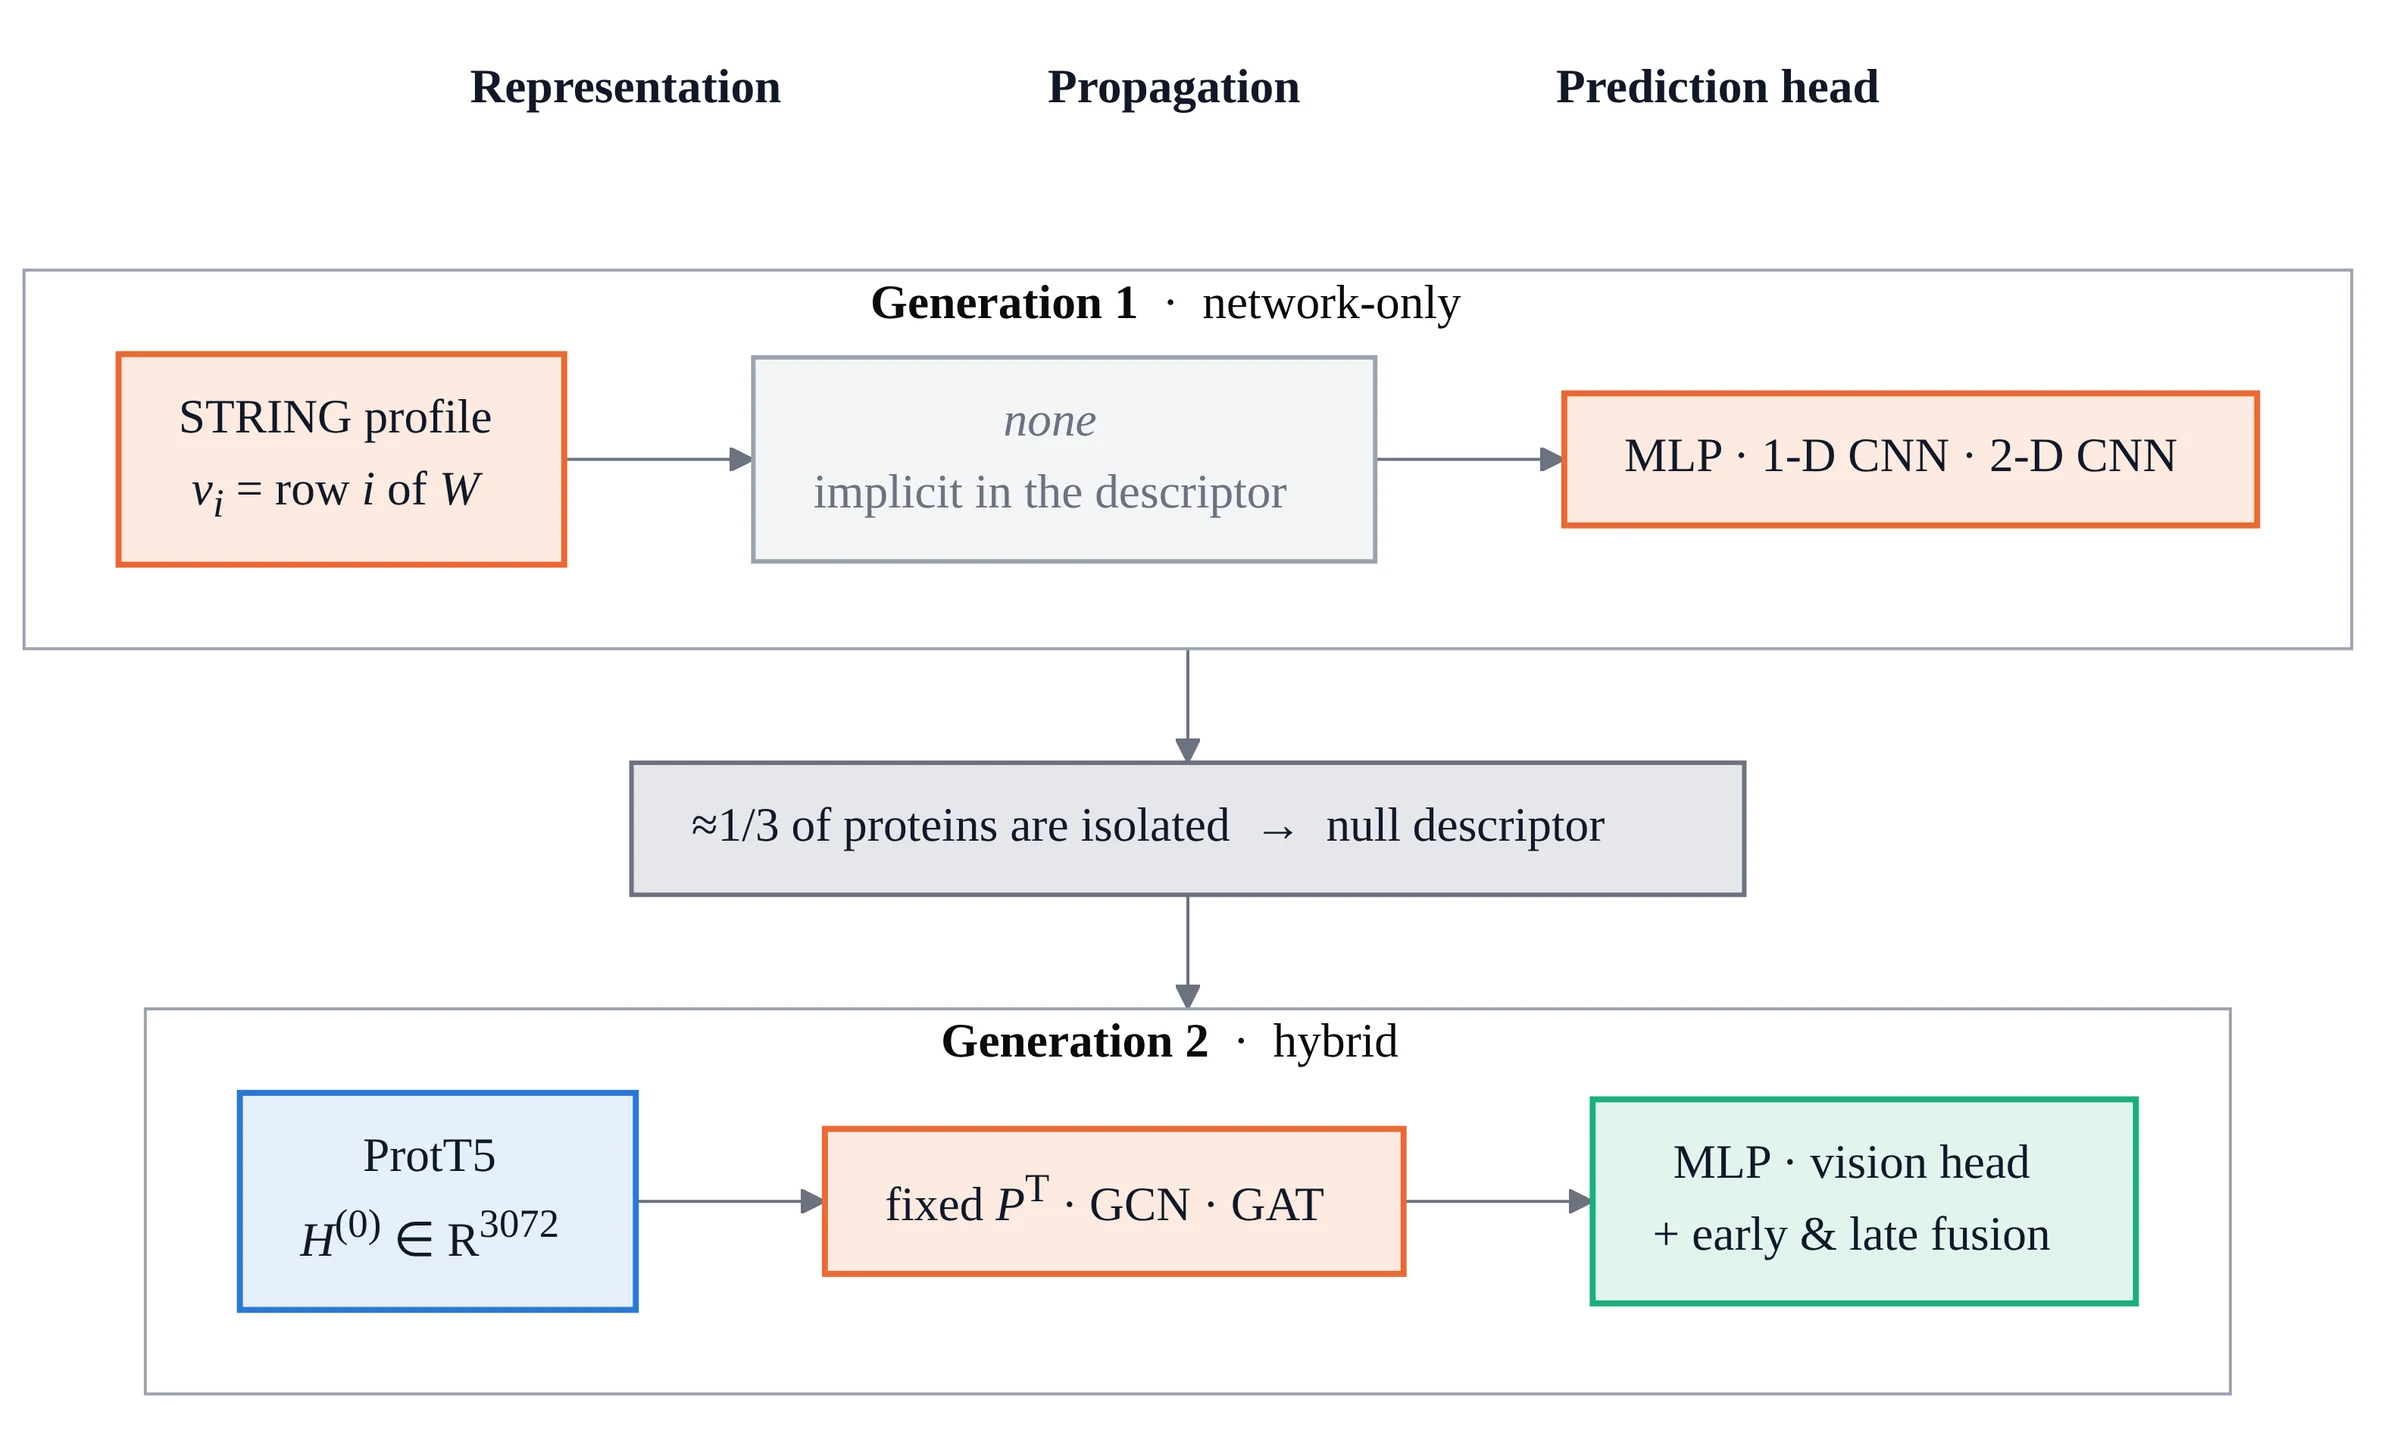
\includegraphics[width=896.7\px,height=535.4\px]{figures/fig_5_1.png}};
\fill<2>[plate] (109,315.3) rectangle ++(896.7,182);
\fill<2-3>[plate] (109,497.3) rectangle ++(896.7,91);
\fill<2-4>[plate] (109,588.3) rectangle ++(896.7,182);
\node[tl] at (88,70) {\fmR\fz{16}{16}\color{inkii}\ls{2}\Ll{4 · Method}};
\node[tl] at (88,131) {\fdA\fz{54}{56.7}\color{ink}\ls{-1}\Ll{Two generations, three decisions}};
\node<2-5>[tl] at (88,808.4) {\fmR\fz{15}{19.5}\color{muted}\Ll{Dissertation, Fig. 5.1}};
\node<2-5>[tl] at (1094.7,236) {\fbR\fz{30}{40.5}\color{ink}\Ll{Representation $\rightarrow$ Propagation\\$\rightarrow$ Prediction head}};
\node<3-5>[tl] at (1094.7,339) {\fbR\fz{30}{40.5}\color{ink}\Ll{Generation 1: network only}};
\node<5>[tl] at (1094.7,401.5) {\fbR\fz{30}{40.5}\color{ink}\Ll{Generation 2 (NEXUS-GO):\\ProtT5 + network}};
\node[tr] at (1512,876) {\fmR\fz{16}{16}\color{muted}18 / 45};
\end{tikzpicture}
\note{Every model decomposes into the same three decisions: representation, propagation and prediction head. 

The limitation of the first generation is a property of its input, about one third of the proteins get a null descriptor, and it motivates the second.}
\end{frame}

\begin{frame}[plain]
\begin{tikzpicture}[deck]
\node<1>[box] at (0,0) {\includegraphics[page=3,width=1600\px]{build/layers}};
\node<2>[box] at (0,0) {\includegraphics[page=53,width=1600\px]{build/layers}};
\node<3>[box] at (0,0) {\includegraphics[page=54,width=1600\px]{build/layers}};
\node<4>[box] at (0,0) {\includegraphics[page=55,width=1600\px]{build/layers}};
\node<2-4>[box] at (109,235) {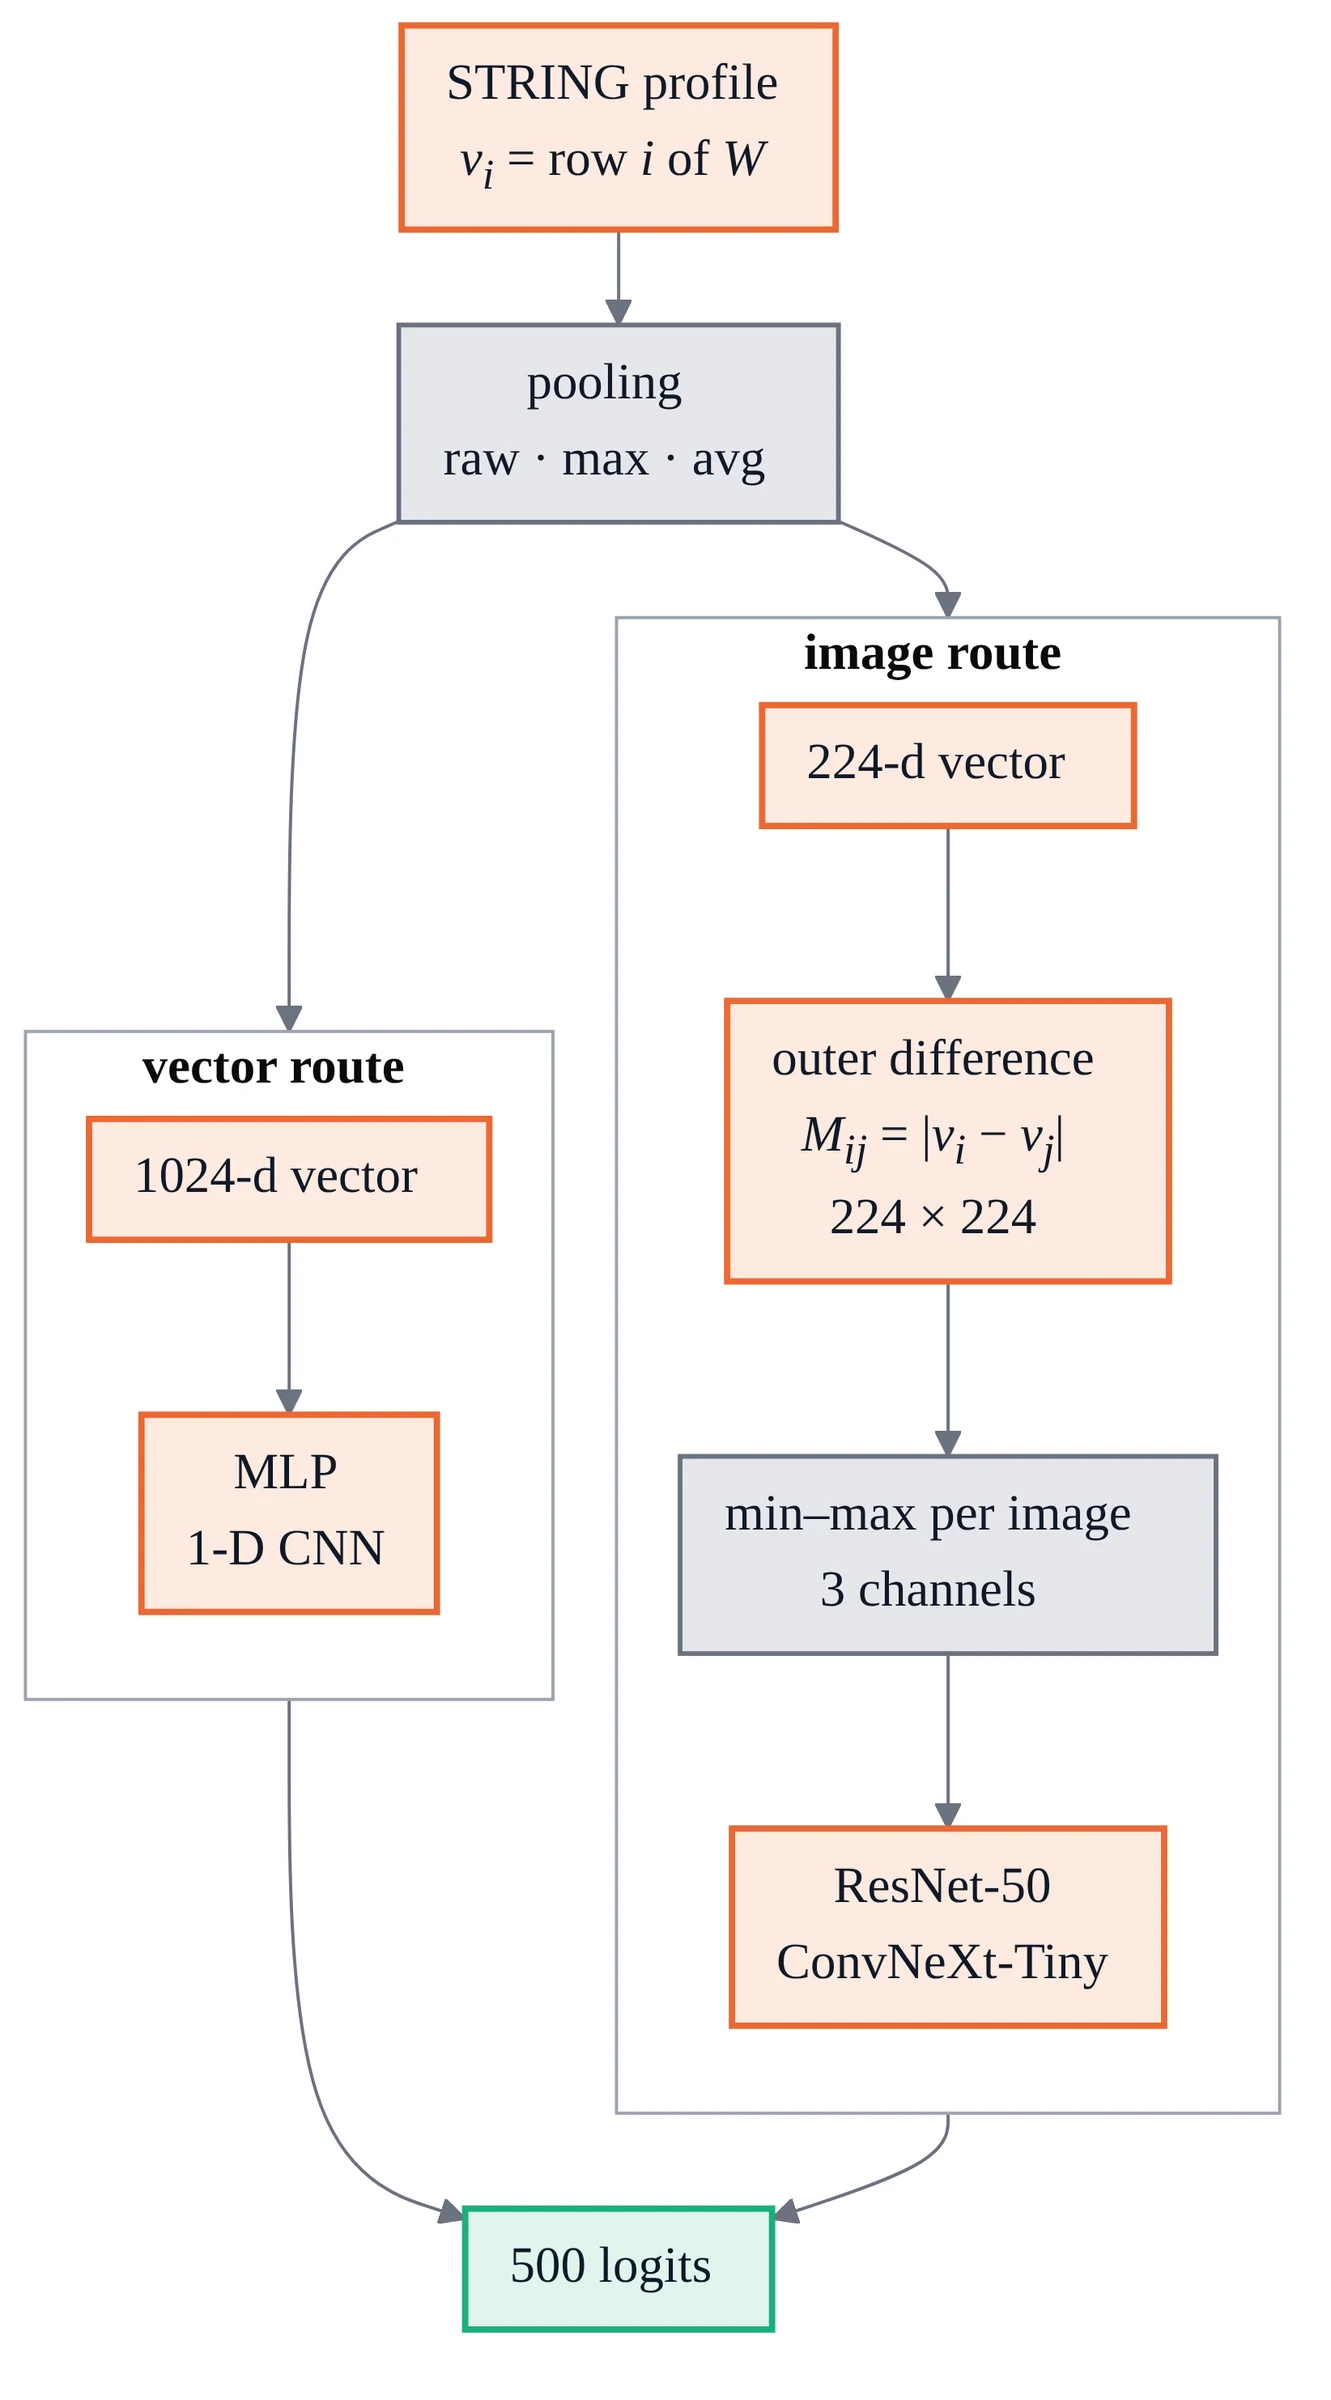
\includegraphics[width=299.5\px,height=540\px]{figures/fig_5_3.png}};
\node<4>[box] at (473,512.5) {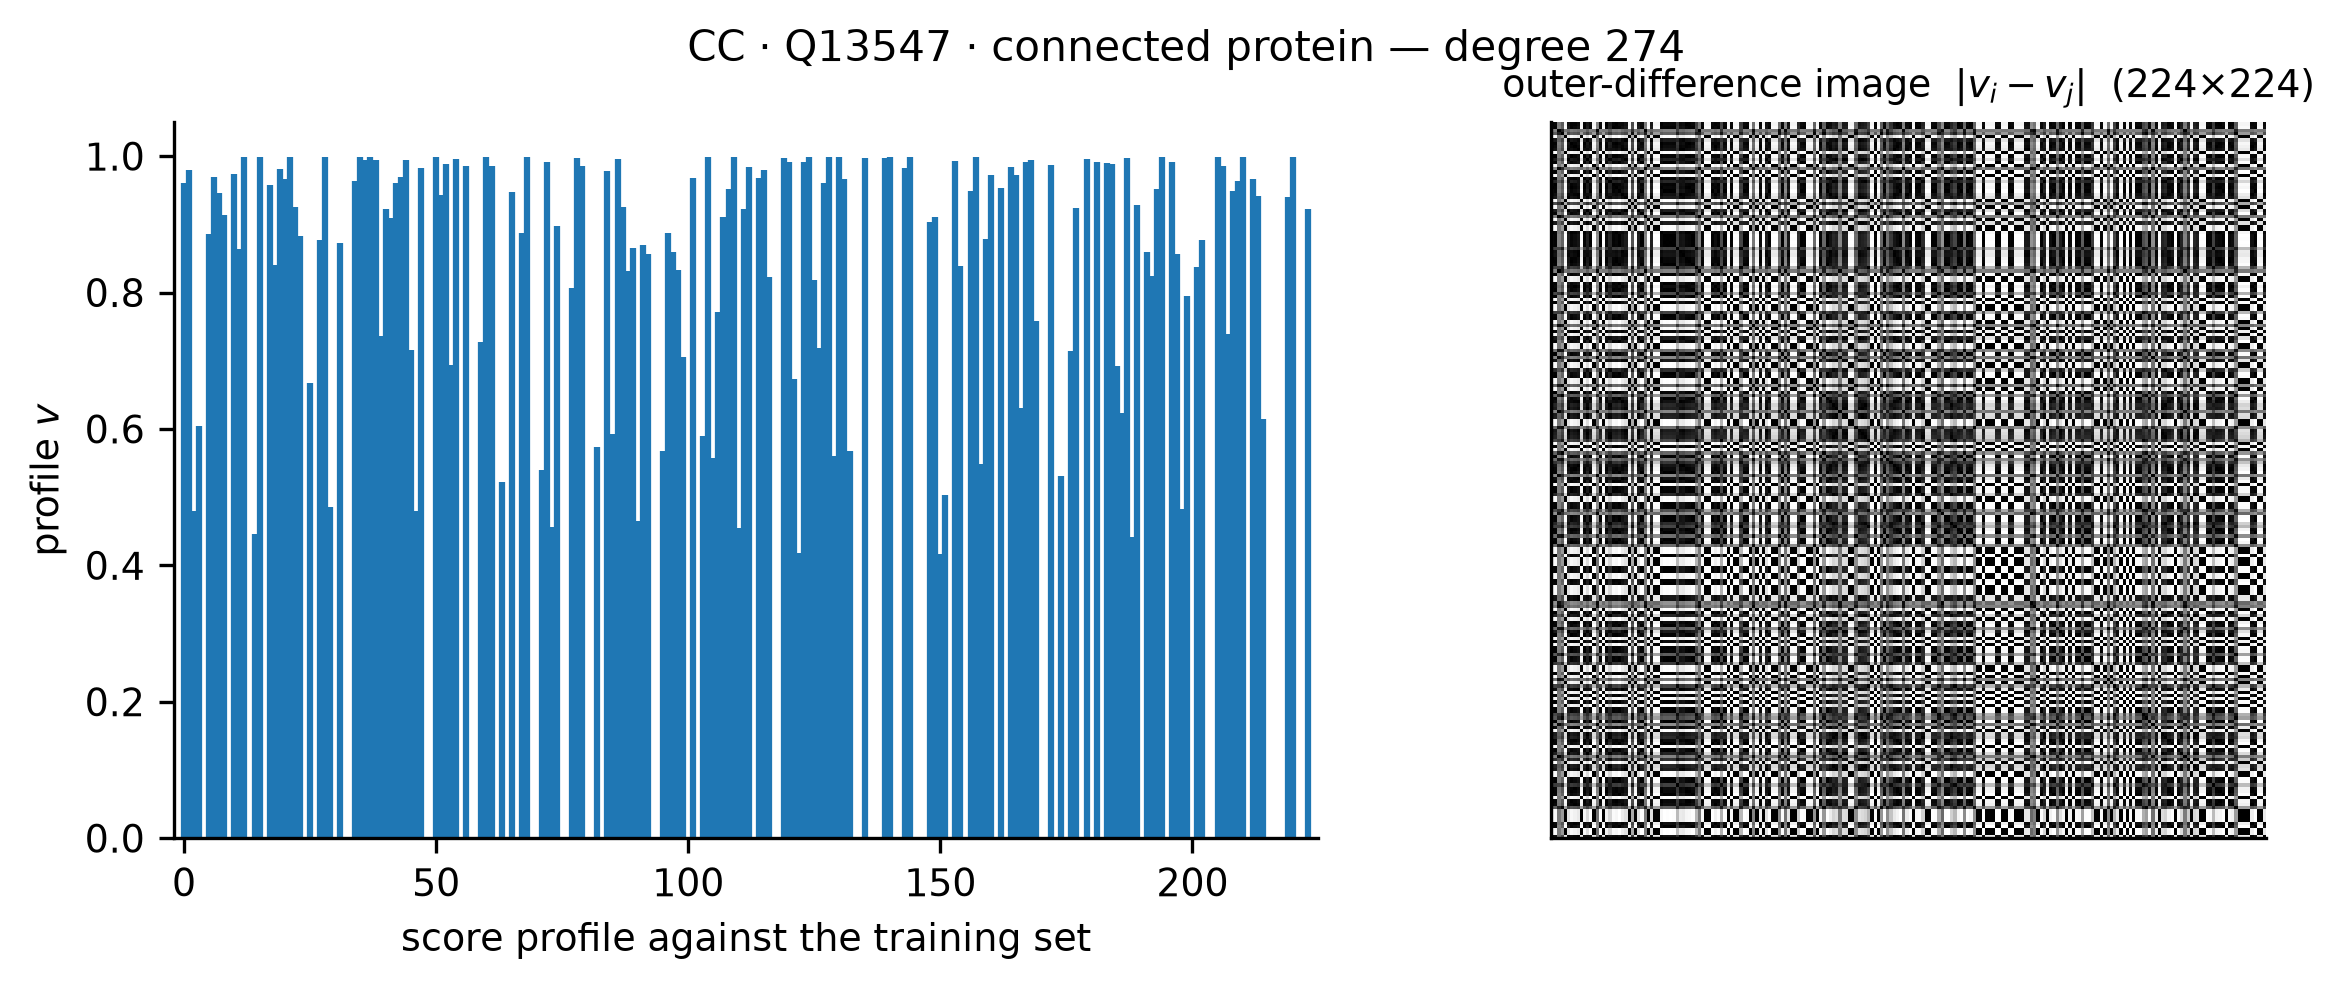
\includegraphics[width=592.2\px,height=250\px]{figures/fig_5_4.png}};
\node[tl] at (88,70) {\fmR\fz{16}{16}\color{inkii}\ls{2}\Ll{4 · Method}};
\node[tl] at (88,131) {\fdA\fz{54}{56.7}\color{ink}\ls{-1}\Ll{Generation 1: the network alone}};
\node<2-4>[tl] at (88,813) {\fmR\fz{15}{19.5}\color{muted}\Ll{Dissertation, Fig. 5.3}};
\node<2-4>[tl] at (488,232) {\fbR\fz{26}{35.1}\color{ink}\Ll{Input: row of the weighted adjacency, against training proteins}};
\node<2-4>[tl] at (488,283.1) {\fbR\fz{26}{35.1}\color{ink}\Ll{Pooling: raw, max, avg}};
\node<3-4>[tl] at (488,334.2) {\fbR\fz{26}{35.1}\color{ink}\Ll{Vector route: MLP or 1-D CNN}};
\node<4>[tl] at (488,385.3) {\fbR\fz{26}{35.1}\color{ink}\Ll{Image route: outer-difference matrix {\fz{29.2}{35}$|v_i - v_j|$}, 224 × 224, ResNet-50 or ConvNeXt-Tiny}};
\node<4>[tl] at (488,436.4) {\fbR\fz{26}{35.1}\color{ink}\Ll{Floor: a naive guilt-by-association baseline}};
\node<4>[tl] at (452,800.5) {\fmR\fz{15}{19.5}\color{muted}\Ll{Dissertation, Fig. 5.4}};
\node[tr] at (1512,876) {\fmR\fz{16}{16}\color{muted}19 / 45};
\end{tikzpicture}
\note{The descriptor is already a one-hop aggregation, so there is no separate propagation stage. 

The image route imports a convolutional bias into a non-visual vector, as SUPERMAGOv2 and DeepInsight did with isolated descriptors.}
\end{frame}

\begin{frame}[plain]
\begin{tikzpicture}[deck]
\node<1>[box] at (0,0) {\includegraphics[page=3,width=1600\px]{build/layers}};
\node<2>[box] at (0,0) {\includegraphics[page=56,width=1600\px]{build/layers}};
\node<3>[box] at (0,0) {\includegraphics[page=57,width=1600\px]{build/layers}};
\node<4>[box] at (0,0) {\includegraphics[page=58,width=1600\px]{build/layers}};
\node<2-4>[box] at (109,235) {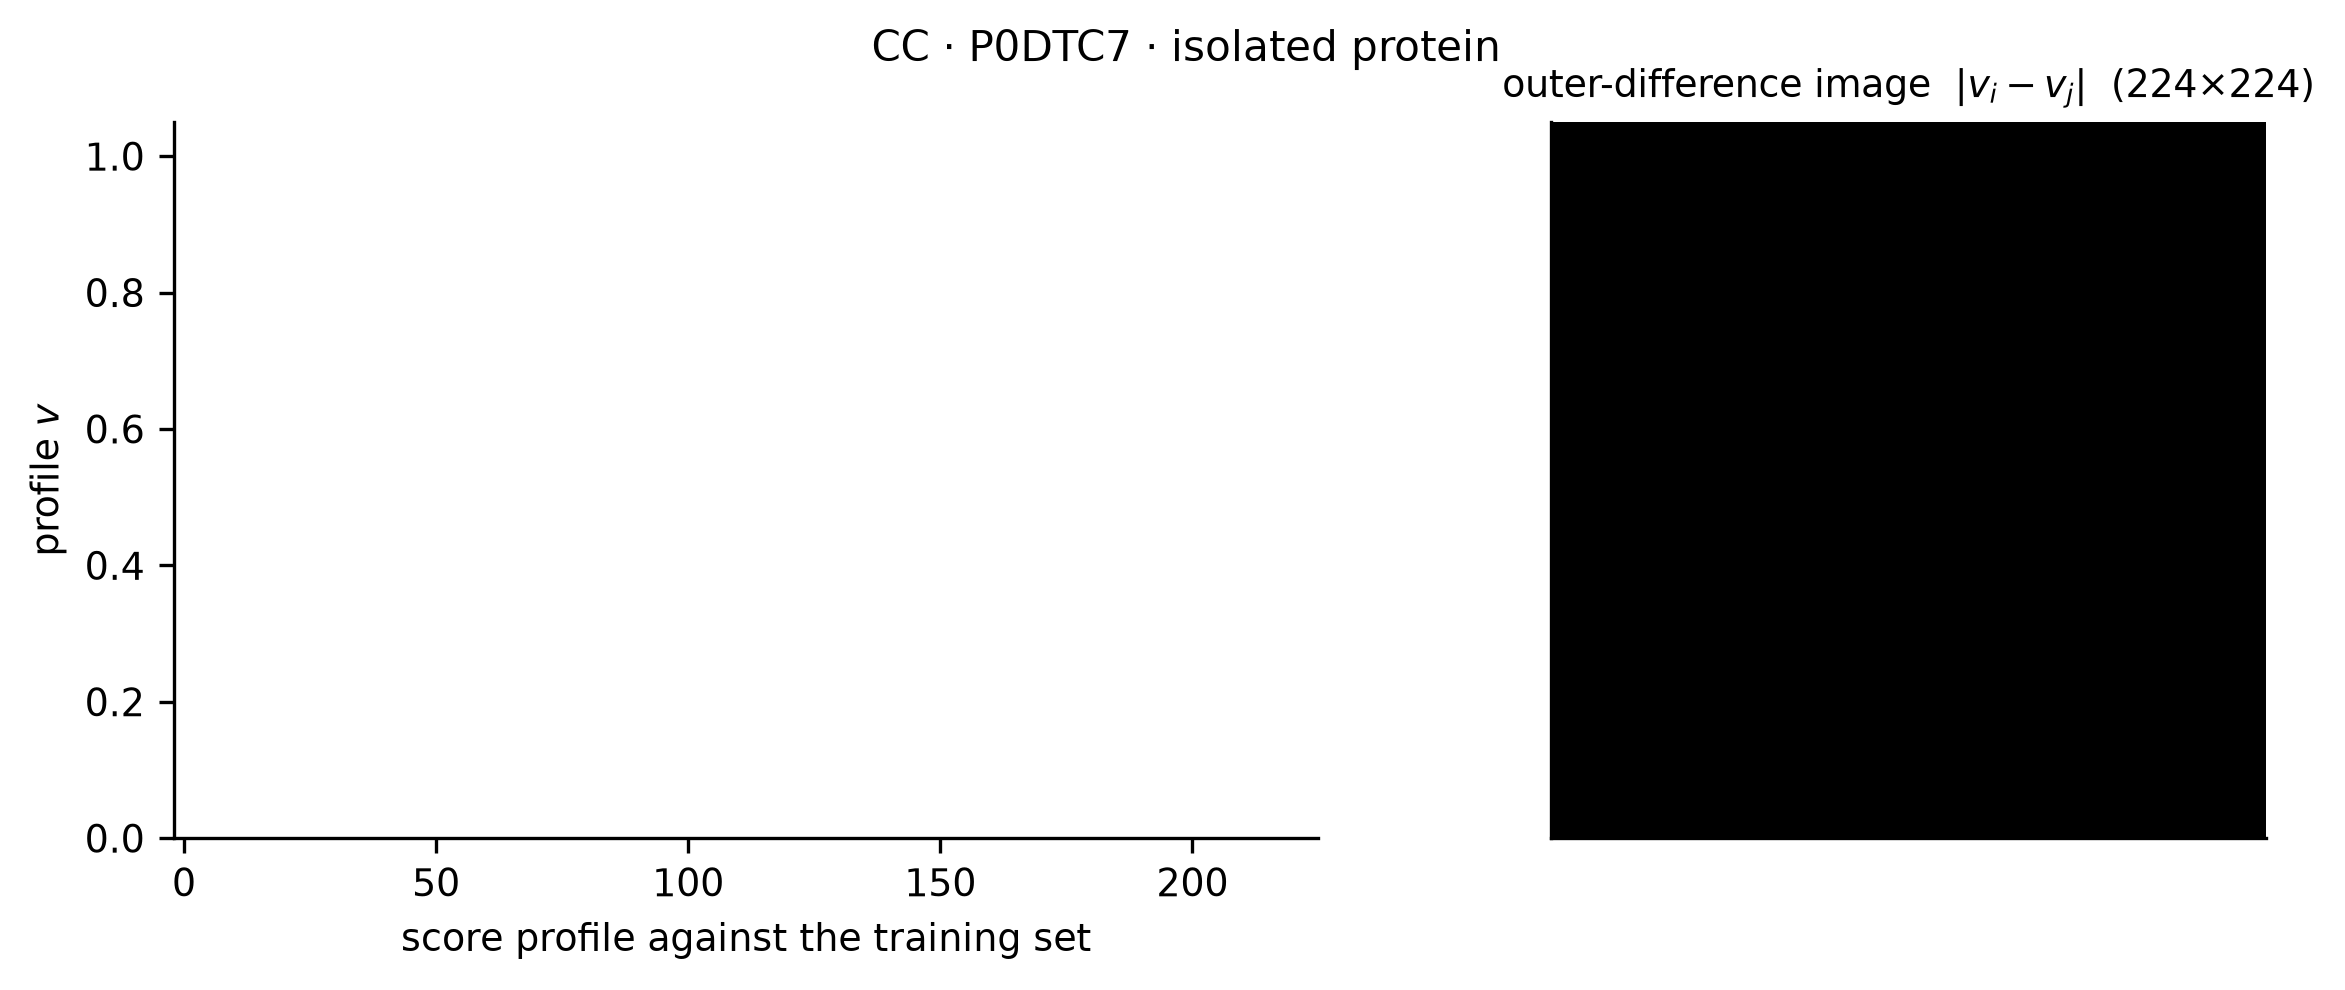
\includegraphics[width=654\px,height=276.1\px]{figures/fig_5_5.png}};
\node<2-4>[box] at (837,235) {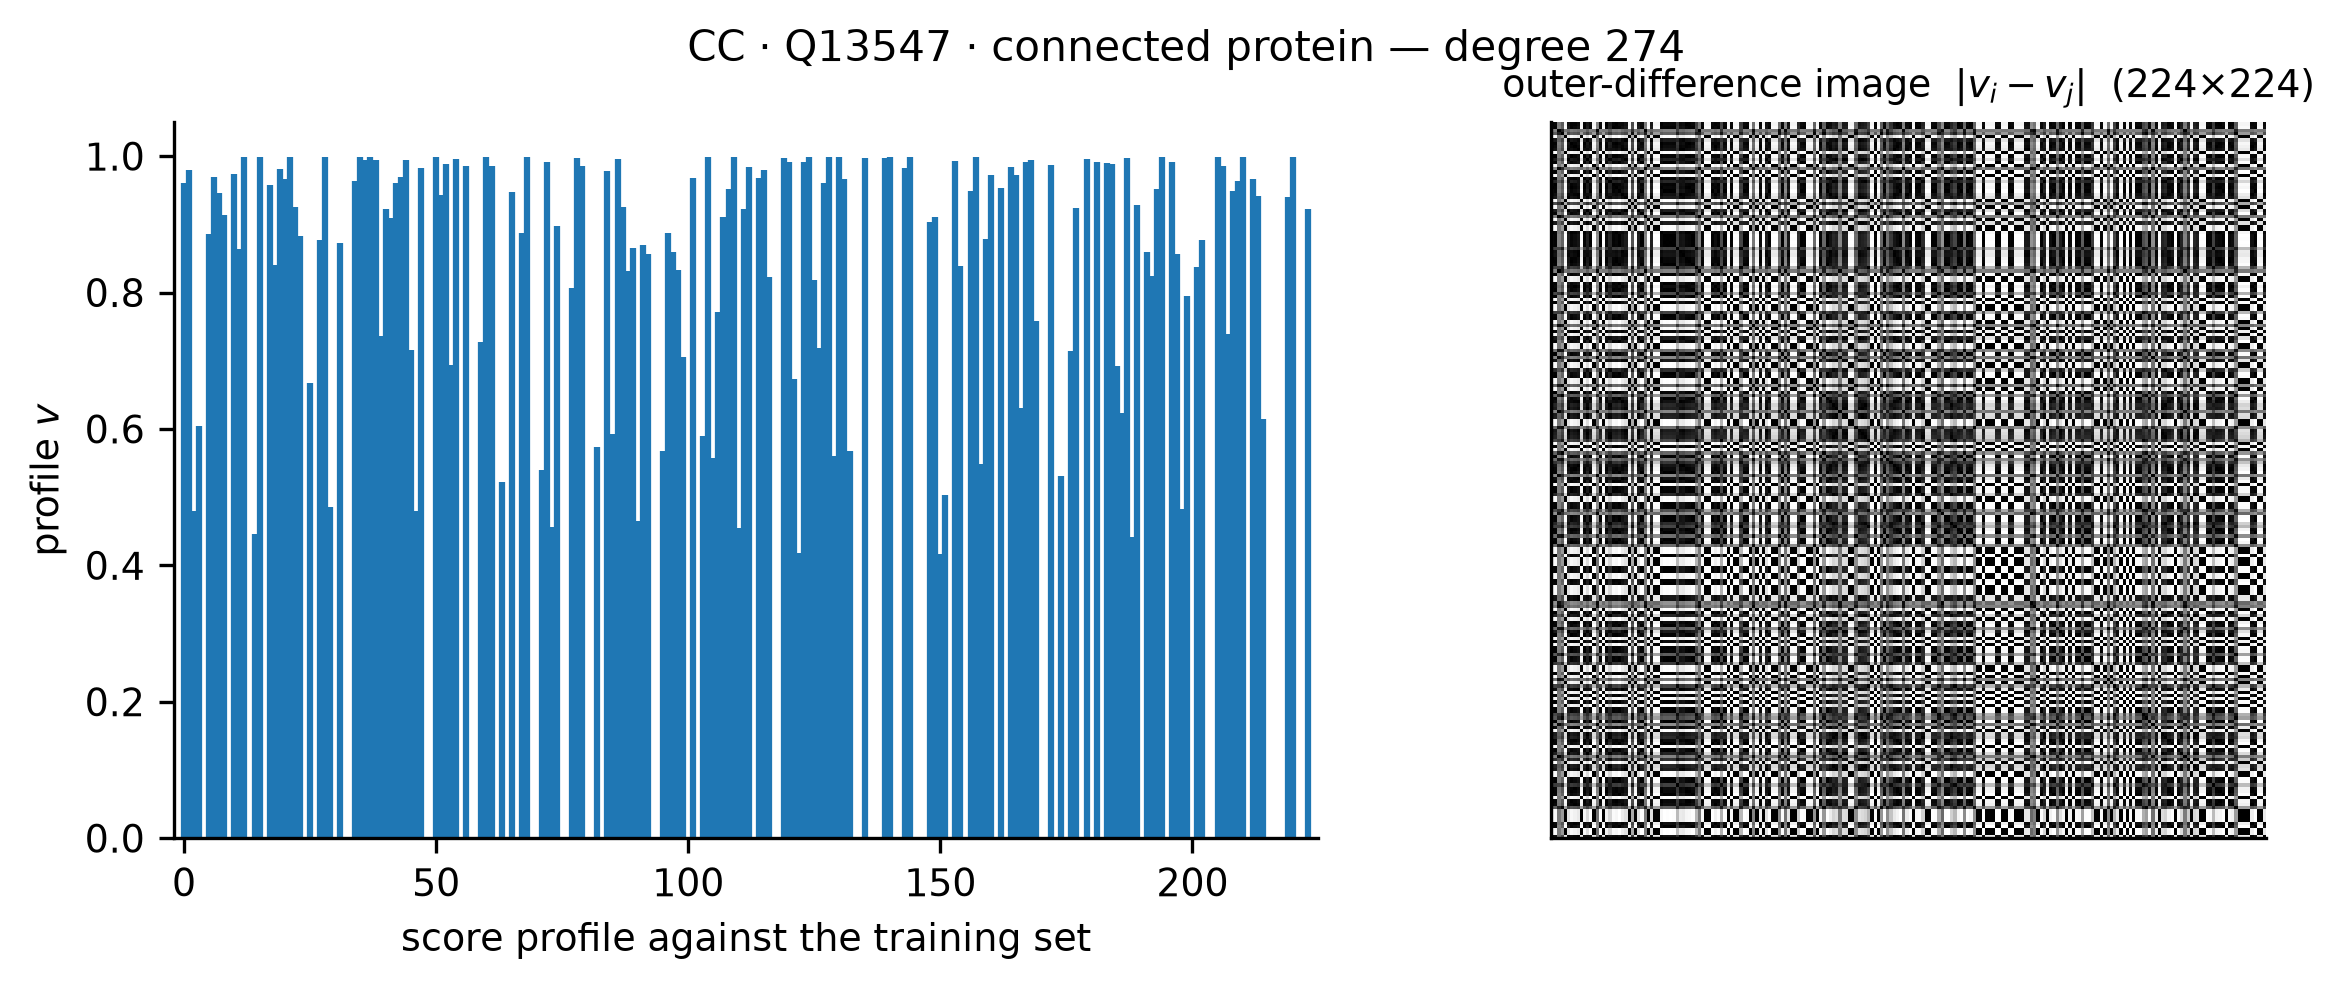
\includegraphics[width=654\px,height=276.1\px]{figures/fig_5_4.png}};
\node[tl] at (88,70) {\fmR\fz{16}{16}\color{inkii}\ls{2}\Ll{4 · Method}};
\node[tl] at (88,131) {\fdA\fz{54}{56.7}\color{ink}\ls{-1}\Ll{An isolated protein has no input}};
\node<2-4>[tl] at (88,549.1) {\fmR\fz{15}{19.5}\color{muted}\Ll{Dissertation, Fig. 5.5 · isolated vs connected}};
\node<2-4>[tl] at (816,549.1) {\fmR\fz{15}{19.5}\color{muted}\Ll{Dissertation, Fig. 5.4 · for contrast}};
\node<3-4>[tl] at (124,583.3) {\fbR\fz{30}{40.5}\color{ink}\Ll{Null profile $\rightarrow$ null matrix $\rightarrow$ uniform image}};
\node<3-4>[tl] at (124,645.8) {\fbR\fz{30}{40.5}\color{ink}\Ll{The head can only return the class prior}};
\node<3-4>[tl] at (124,708.3) {\fbR\fz{30}{40.5}\color{ink}\Ll{No architecture can recover what is absent}};
\node<4>[tl] at (846,779.8) {\fdA\fz{38}{45.6}\color{ink}\Ll{Requirement: a representation\\that exists for every protein}};
\node[tr] at (1512,876) {\fmR\fz{16}{16}\color{muted}20 / 45};
\end{tikzpicture}
\note{For a third of the corpus the first generation sees nothing. 

The amino-acid sequence satisfies the requirement by construction, and that is where the second generation starts.}
\end{frame}

\begin{frame}[plain]
\hypertarget<1>{s21.1}{}
\hypertarget<2>{s21.2}{}
\hypertarget<3>{s21.3}{}
\hypertarget<4>{s21.4}{}
\hypertarget<5>{s21.5}{}
\hypertarget<6>{s21.6}{}
\hypertarget<7>{s21.7}{}
\hypertarget<8>{s21.8}{}
\begin{tikzpicture}[deck]
\node<1>[box] at (0,0) {\includegraphics[page=59,width=1600\px]{build/layers}};
\node<2>[box] at (0,0) {\includegraphics[page=60,width=1600\px]{build/layers}};
\node<3>[box] at (0,0) {\includegraphics[page=61,width=1600\px]{build/layers}};
\node<4>[box] at (0,0) {\includegraphics[page=62,width=1600\px]{build/layers}};
\node<5>[box] at (0,0) {\includegraphics[page=63,width=1600\px]{build/layers}};
\node<6>[box] at (0,0) {\includegraphics[page=64,width=1600\px]{build/layers}};
\node<7>[box] at (0,0) {\includegraphics[page=65,width=1600\px]{build/layers}};
\node<8>[box] at (0,0) {\includegraphics[page=66,width=1600\px]{build/layers}};
\node<4-8>[box] at (207.4,206) {\hot{89.1}{42}{s21.4}};
\node<4-8>[box] at (295,206) {\hot{82.5}{42}{s21.5}};
\node<4-8>[box] at (376,206) {\hot{84.8}{42}{s21.6}};
\node<4-8>[box] at (459.4,206) {\hot{80}{42}{s21.7}};
\node<4-8>[box] at (152,206) {\hot{56.9}{42}{s21.8}};
\node<4-8>[box] at (1315.5,206) {\hot{196.5}{42}{s21fig}};
\fill<8>[slide] (86,204) rectangle ++(1428,544); \node<8>[box] at (88,206) {\animategraphics[autoplay,loop,width=1424\px]{10}{build/seq/pipe-anim}{}{}};
\node[tl] at (88,70) {\fmR\fz{16}{16}\color{inkii}\ls{2}\Ll{4 · Method}};
\node[tl] at (88,131) {\fdA\fz{54}{56.7}\color{ink}\ls{-1}\Ll{NEXUS-GO: four routes}};
\node<2-8>[tl] at (88,803.1) {\fbR\fz{24}{31.2}\color{ink}\Ll{Sequence $\rightarrow$ ProtT5 $\rightarrow$ {\fz{26.9}{32.3}$\mathbf{H}^{(0)} \in \mathbb{R}^{3072}$}}};
\node<3-8>[tl] at (573.3,802) {\fbR\fz{24}{31.2}\color{ink}\Ll{STRING $\rightarrow$ weighted graph {\fz{26.9}{32.3}$W$} $\rightarrow$\\{\fz{26.9}{32.3}$P = W D_c^{-1}$}}};
\node<4-8>[tl] at (1058.7,802) {\fbR\fz{24}{31.2}\color{ink}\Ll{Routes: /Fixed · /GNN · /Early · /Late}};
\node[tr] at (1512,876) {\fmR\fz{16}{16}\color{muted}21 / 45};
\end{tikzpicture}
\note{Two inputs, two propagation routes and two ways of combining them. 

The first generation is reported as a topology-only control and carries no route name.}
\end{frame}

\begin{frame}[plain]
\begin{tikzpicture}[deck]
\node<1>[box] at (0,0) {\includegraphics[page=3,width=1600\px]{build/layers}};
\node<2>[box] at (0,0) {\includegraphics[page=67,width=1600\px]{build/layers}};
\node<3>[box] at (0,0) {\includegraphics[page=68,width=1600\px]{build/layers}};
\node<4>[box] at (0,0) {\includegraphics[page=69,width=1600\px]{build/layers}};
\node<2-4>[box] at (109,235) {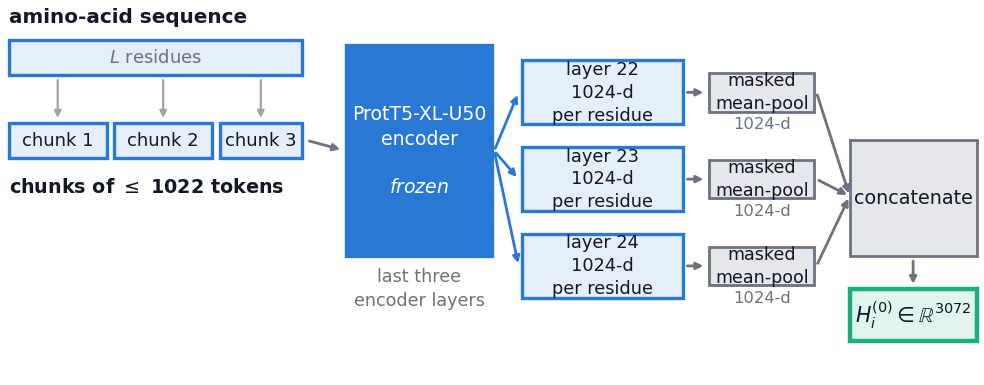
\includegraphics[width=1022.3\px,height=400\px]{figures/fig_5_7.png}};
\node[tl] at (88,70) {\fmR\fz{16}{16}\color{inkii}\ls{2}\Ll{4 · Method}};
\node[tl] at (88,131) {\fdA\fz{54}{56.7}\color{ink}\ls{-1}\Ll{ProtT5-XL-U50, three layers, frozen}};
\node<2-4>[tl] at (88,673) {\fmR\fz{15}{19.5}\color{muted}\Ll{Dissertation, Fig. 5.7}};
\node<2-4>[tl] at (124,729.5) {\fbR\fz{26}{35.1}\color{ink}\Ll{Chunks of at most 1,022 residues;\\masked mean-pool, then mean\\over chunks}};
\node<3-4>[tl] at (609.3,729.5) {\fbR\fz{26}{35.1}\color{ink}\Ll{Layers 24, 23, 22, concatenated: 3 ×\\1024 = 3072 dimensions}};
\node<4>[tl] at (1094.7,729.5) {\fbR\fz{26}{35.1}\color{ink}\Ll{Exists for every protein, isolated\\or not}};
\node[tr] at (1512,876) {\fmR\fz{16}{16}\color{muted}22 / 45};
\end{tikzpicture}
\note{Reading three adjacent layers avoids committing to one point between the pretraining objective and structural signal, at no tuning cost. 

Extraction is inherited from SUPERMAGOv2.}
\end{frame}

\begin{frame}[plain]
\hypertarget<1>{s23.1}{}
\hypertarget<2>{s23.2}{}
\hypertarget<3>{s23.3}{}
\hypertarget<4>{s23.4}{}
\hypertarget<5>{s23.5}{}
\begin{tikzpicture}[deck]
\node<1>[box] at (0,0) {\includegraphics[page=3,width=1600\px]{build/layers}};
\node<2>[box] at (0,0) {\includegraphics[page=70,width=1600\px]{build/layers}};
\node<3>[box] at (0,0) {\includegraphics[page=71,width=1600\px]{build/layers}};
\node<4>[box] at (0,0) {\includegraphics[page=72,width=1600\px]{build/layers}};
\node<5>[box] at (0,0) {\includegraphics[page=73,width=1600\px]{build/layers}};
\node<3-5>[box] at (749.1,206) {\hot{71.1}{42}{s23.4}};
\node<3-5>[box] at (818.7,206) {\hot{71}{42}{s23.5}};
\node[tl] at (88,70) {\fmR\fz{16}{16}\color{inkii}\ls{2}\Ll{4 · Method}};
\node[tl] at (88,131) {\fdA\fz{54}{56.7}\color{ink}\ls{-1}\Ll{From records to an operator}};
\node<2-5>[tl] at (124,236) {\fbR\fz{30}{40.5}\color{ink}\Ll{Symmetric, no self-loops, sparse COO: at\\most 1,133,132 stored entries (dense: 25\\to 35 GB)}};
\node<3-5>[tl] at (124,379.5) {\fbR\fz{30}{40.5}\color{ink}\Ll{Deduplication: max keeps the score;\\sum multiplies it by the record count}};
\node<4-5>[tl] at (124,482.5) {\fbR\fz{30}{40.5}\color{ink}\Ll{Column-stochastic {\fz{33.7}{40.4}$P = W D_c^{-1}$}: weights\\are relative to each protein's neighbours}};
\node[tr] at (1512,876) {\fmR\fz{16}{16}\color{muted}23 / 45};
\end{tikzpicture}
\note{Repeated records carry no extra score, so summing rewards how often a pair was written down. The maximum keeps the STRING score on its own scale. 

Normalization does not undo the reordering.}
\end{frame}

\begin{frame}[plain]
\hypertarget<1>{s24.1}{}
\hypertarget<2>{s24.2}{}
\hypertarget<3>{s24.3}{}
\hypertarget<4>{s24.4}{}
\hypertarget<5>{s24.5}{}
\hypertarget<6>{s24.6}{}
\hypertarget<7>{s24.7}{}
\hypertarget<8>{s24.8}{}
\begin{tikzpicture}[deck]
\node<1-2>[box] at (0,0) {\includegraphics[page=3,width=1600\px]{build/layers}};
\node<3>[box] at (0,0) {\includegraphics[page=74,width=1600\px]{build/layers}};
\node<4>[box] at (0,0) {\includegraphics[page=75,width=1600\px]{build/layers}};
\node<5,8>[box] at (0,0) {\includegraphics[page=76,width=1600\px]{build/layers}};
\node<6>[box] at (0,0) {\includegraphics[page=77,width=1600\px]{build/layers}};
\node<7>[box] at (0,0) {\includegraphics[page=78,width=1600\px]{build/layers}};
\node<3>[box] at (800.2,211) {\hot{13.6}{32}{s24.6}};
\node<3>[box] at (813.9,211) {\hot{11.2}{32}{s24x.46}};
\node<3>[box] at (825,211) {\hot{11.2}{32}{s24.5}};
\node<3>[box] at (836.2,211) {\hot{11.2}{32}{s24x.48}};
\node<3>[box] at (847.5,211) {\hot{11.2}{32}{s24x.49}};
\node<3>[box] at (858.6,211) {\hot{11.2}{32}{s24x.50}};
\node<3>[box] at (869.9,211) {\hot{11.2}{32}{s24.7}};
\node<3>[box] at (881,211) {\hot{11.2}{32}{s24x.52}};
\node<3>[box] at (892.2,211) {\hot{11.2}{32}{s24x.53}};
\node<3>[box] at (903.5,211) {\hot{11.2}{32}{s24x.54}};
\node<3>[box] at (914.6,211) {\hot{13.6}{32}{s24x.55}};
\node<3>[box] at (1139.7,211) {\hot{15}{32}{s24x.3}};
\node<3>[box] at (1154.7,211) {\hot{14}{32}{s24x.14}};
\node<3>[box] at (1168.7,211) {\hot{14}{32}{s24x.25}};
\node<3>[box] at (1182.7,211) {\hot{14}{32}{s24x.36}};
\node<3>[box] at (1196.7,211) {\hot{14}{32}{s24.5}};
\node<3>[box] at (1210.7,211) {\hot{14}{32}{s24x.58}};
\node<3>[box] at (1224.7,211) {\hot{14}{32}{s24x.69}};
\node<3>[box] at (1238.7,211) {\hot{14}{32}{s24x.80}};
\node<3>[box] at (1252.7,211) {\hot{15}{32}{s24x.91}};
\node<3>[box] at (1337.3,206) {\hot{70.2}{42}{s24.8}};
\node<4>[box] at (800.2,211) {\hot{13.6}{32}{s24.6}};
\node<4>[box] at (813.9,211) {\hot{11.2}{32}{s24x.46}};
\node<4>[box] at (825,211) {\hot{11.2}{32}{s24.5}};
\node<4>[box] at (836.2,211) {\hot{11.2}{32}{s24x.48}};
\node<4>[box] at (847.5,211) {\hot{11.2}{32}{s24x.49}};
\node<4>[box] at (858.6,211) {\hot{11.2}{32}{s24x.50}};
\node<4>[box] at (869.9,211) {\hot{11.2}{32}{s24.7}};
\node<4>[box] at (881,211) {\hot{11.2}{32}{s24x.52}};
\node<4>[box] at (892.2,211) {\hot{11.2}{32}{s24x.53}};
\node<4>[box] at (903.5,211) {\hot{11.2}{32}{s24x.54}};
\node<4>[box] at (914.6,211) {\hot{13.6}{32}{s24x.55}};
\node<4>[box] at (1139.7,211) {\hot{15}{32}{s24x.3}};
\node<4>[box] at (1154.7,211) {\hot{14}{32}{s24x.14}};
\node<4>[box] at (1168.7,211) {\hot{14}{32}{s24x.25}};
\node<4>[box] at (1182.7,211) {\hot{14}{32}{s24x.36}};
\node<4>[box] at (1196.7,211) {\hot{14}{32}{s24.5}};
\node<4>[box] at (1210.7,211) {\hot{14}{32}{s24x.58}};
\node<4>[box] at (1224.7,211) {\hot{14}{32}{s24x.69}};
\node<4>[box] at (1238.7,211) {\hot{14}{32}{s24x.80}};
\node<4>[box] at (1252.7,211) {\hot{15}{32}{s24x.91}};
\node<4>[box] at (1337.3,206) {\hot{70.2}{42}{s24.8}};
\node<5>[box] at (800.2,211) {\hot{13.6}{32}{s24.6}};
\node<5>[box] at (813.9,211) {\hot{11.2}{32}{s24x.46}};
\node<5>[box] at (825,211) {\hot{11.2}{32}{s24.5}};
\node<5>[box] at (836.2,211) {\hot{11.2}{32}{s24x.48}};
\node<5>[box] at (847.5,211) {\hot{11.2}{32}{s24x.49}};
\node<5>[box] at (858.6,211) {\hot{11.2}{32}{s24x.50}};
\node<5>[box] at (869.9,211) {\hot{11.2}{32}{s24.7}};
\node<5>[box] at (881,211) {\hot{11.2}{32}{s24x.52}};
\node<5>[box] at (892.2,211) {\hot{11.2}{32}{s24x.53}};
\node<5>[box] at (903.5,211) {\hot{11.2}{32}{s24x.54}};
\node<5>[box] at (914.6,211) {\hot{13.6}{32}{s24x.55}};
\node<5>[box] at (1139.7,211) {\hot{15}{32}{s24x.3}};
\node<5>[box] at (1154.7,211) {\hot{14}{32}{s24x.14}};
\node<5>[box] at (1168.7,211) {\hot{14}{32}{s24x.25}};
\node<5>[box] at (1182.7,211) {\hot{14}{32}{s24x.36}};
\node<5>[box] at (1196.7,211) {\hot{14}{32}{s24.5}};
\node<5>[box] at (1210.7,211) {\hot{14}{32}{s24x.58}};
\node<5>[box] at (1224.7,211) {\hot{14}{32}{s24x.69}};
\node<5>[box] at (1238.7,211) {\hot{14}{32}{s24x.80}};
\node<5>[box] at (1252.7,211) {\hot{15}{32}{s24x.91}};
\node<5>[box] at (1337.3,206) {\hot{70.2}{42}{s24.8}};
\node<6>[box] at (800.2,211) {\hot{13.6}{32}{s24.6}};
\node<6>[box] at (813.9,211) {\hot{11.2}{32}{s24x.46}};
\node<6>[box] at (825,211) {\hot{11.2}{32}{s24.5}};
\node<6>[box] at (836.2,211) {\hot{11.2}{32}{s24x.48}};
\node<6>[box] at (847.5,211) {\hot{11.2}{32}{s24x.49}};
\node<6>[box] at (858.6,211) {\hot{11.2}{32}{s24x.50}};
\node<6>[box] at (869.9,211) {\hot{11.2}{32}{s24.7}};
\node<6>[box] at (881,211) {\hot{11.2}{32}{s24x.52}};
\node<6>[box] at (892.2,211) {\hot{11.2}{32}{s24x.53}};
\node<6>[box] at (903.5,211) {\hot{11.2}{32}{s24x.54}};
\node<6>[box] at (914.6,211) {\hot{13.6}{32}{s24x.55}};
\node<6>[box] at (1139.7,211) {\hot{15}{32}{s24x.1}};
\node<6>[box] at (1154.7,211) {\hot{14}{32}{s24x.12}};
\node<6>[box] at (1168.7,211) {\hot{14}{32}{s24x.23}};
\node<6>[box] at (1182.7,211) {\hot{14}{32}{s24x.34}};
\node<6>[box] at (1196.7,211) {\hot{14}{32}{s24.6}};
\node<6>[box] at (1210.7,211) {\hot{14}{32}{s24x.56}};
\node<6>[box] at (1224.7,211) {\hot{14}{32}{s24x.67}};
\node<6>[box] at (1238.7,211) {\hot{14}{32}{s24x.78}};
\node<6>[box] at (1252.7,211) {\hot{15}{32}{s24x.89}};
\node<6>[box] at (1337.3,206) {\hot{70.2}{42}{s24.8}};
\node<7>[box] at (800.2,211) {\hot{13.6}{32}{s24.6}};
\node<7>[box] at (813.9,211) {\hot{11.2}{32}{s24x.46}};
\node<7>[box] at (825,211) {\hot{11.2}{32}{s24.5}};
\node<7>[box] at (836.2,211) {\hot{11.2}{32}{s24x.48}};
\node<7>[box] at (847.5,211) {\hot{11.2}{32}{s24x.49}};
\node<7>[box] at (858.6,211) {\hot{11.2}{32}{s24x.50}};
\node<7>[box] at (869.9,211) {\hot{11.2}{32}{s24.7}};
\node<7>[box] at (881,211) {\hot{11.2}{32}{s24x.52}};
\node<7>[box] at (892.2,211) {\hot{11.2}{32}{s24x.53}};
\node<7>[box] at (903.5,211) {\hot{11.2}{32}{s24x.54}};
\node<7>[box] at (914.6,211) {\hot{13.6}{32}{s24x.55}};
\node<7>[box] at (1139.7,211) {\hot{15}{32}{s24x.7}};
\node<7>[box] at (1154.7,211) {\hot{14}{32}{s24x.18}};
\node<7>[box] at (1168.7,211) {\hot{14}{32}{s24x.29}};
\node<7>[box] at (1182.7,211) {\hot{14}{32}{s24x.40}};
\node<7>[box] at (1196.7,211) {\hot{14}{32}{s24.7}};
\node<7>[box] at (1210.7,211) {\hot{14}{32}{s24x.62}};
\node<7>[box] at (1224.7,211) {\hot{14}{32}{s24x.73}};
\node<7>[box] at (1238.7,211) {\hot{14}{32}{s24x.84}};
\node<7>[box] at (1252.7,211) {\hot{15}{32}{s24x.95}};
\node<7>[box] at (1337.3,206) {\hot{70.2}{42}{s24.8}};
\node<8>[box] at (800.2,211) {\hot{13.6}{32}{s24.6}};
\node<8>[box] at (813.9,211) {\hot{11.2}{32}{s24x.46}};
\node<8>[box] at (825,211) {\hot{11.2}{32}{s24.5}};
\node<8>[box] at (836.2,211) {\hot{11.2}{32}{s24x.48}};
\node<8>[box] at (847.5,211) {\hot{11.2}{32}{s24x.49}};
\node<8>[box] at (858.6,211) {\hot{11.2}{32}{s24x.50}};
\node<8>[box] at (869.9,211) {\hot{11.2}{32}{s24.7}};
\node<8>[box] at (881,211) {\hot{11.2}{32}{s24x.52}};
\node<8>[box] at (892.2,211) {\hot{11.2}{32}{s24x.53}};
\node<8>[box] at (903.5,211) {\hot{11.2}{32}{s24x.54}};
\node<8>[box] at (914.6,211) {\hot{13.6}{32}{s24x.55}};
\node<8>[box] at (1139.7,211) {\hot{15}{32}{s24x.3}};
\node<8>[box] at (1154.7,211) {\hot{14}{32}{s24x.14}};
\node<8>[box] at (1168.7,211) {\hot{14}{32}{s24x.25}};
\node<8>[box] at (1182.7,211) {\hot{14}{32}{s24x.36}};
\node<8>[box] at (1196.7,211) {\hot{14}{32}{s24.5}};
\node<8>[box] at (1210.7,211) {\hot{14}{32}{s24x.58}};
\node<8>[box] at (1224.7,211) {\hot{14}{32}{s24x.69}};
\node<8>[box] at (1238.7,211) {\hot{14}{32}{s24x.80}};
\node<8>[box] at (1252.7,211) {\hot{15}{32}{s24x.91}};
\node<8>[box] at (1337.3,206) {\hot{70.2}{42}{s24.8}};
\fill<8>[slide] (692.7,204) rectangle ++(821.3,634); \node<8>[box] at (694.7,206) {\animategraphics[autoplay,loop,width=817.3\px]{2}{build/seq/prop-anim}{}{}};
\node[tl] at (88,70) {\fmR\fz{16}{16}\color{inkii}\ls{2}\Ll{4 · Method}};
\node[tl] at (88,131) {\fdA\fz{54}{56.7}\color{ink}\ls{-1}\Ll{Fixed propagation: no parameters}};
\node<2-8>[tl] at (88,237.7) {\fbR\fz{30}{36}\color{ink}\Ll{{\fz{33.7}{40.4}$\displaystyle \mathbf{H}^{(h)} = \alpha\, \mathbf{H}^{(h-1)} + (1-\alpha)\, P^{\top} \mathbf{H}^{(h-1)}$}}};
\node<2-8>[tl] at (88,278.2) {\fbR\fz{24}{32.4}\color{inkii}\Ll{{\fz{26.9}{32.3}$h = 1, \dots, T$}}};
\node<4-8>[tl] at (124,346.6) {\fbR\fz{26}{35.1}\color{ink}\Ll{Closed form: hop {\fz{29.2}{35}$k$} gets weight\\[0.9\px]{\fz{29.2}{35}$\binom{T}{k}\, \alpha^{T-k} (1-\alpha)^{k}$}}};
\node<4-8>[tl] at (124,434.9) {\fbR\fz{26}{35.1}\color{ink}\Ll{Computed once, cached, reused every epoch}};
\node<5-8>[tl] at (124,486) {\fbR\fz{26}{35.1}\color{ink}\Ll{{\fz{29.2}{35}$T = 0$} or {\fz{29.2}{35}$\alpha = 1$}: the graph is switched off\\(internal control)}};
\node[tr] at (1512,876) {\fmR\fz{16}{16}\color{muted}24 / 45};
\end{tikzpicture}
\note{$\alpha$ retains part of the previous step, not of the original, so it slows mixing instead of re-injecting the input. 

The weights over hop counts are binomial with mean T(1 − $\alpha$). Unlike personalized PageRank, the initial state is never reintroduced.}
\end{frame}

\begin{frame}[plain]
\begin{tikzpicture}[deck]
\node<1>[box] at (0,0) {\includegraphics[page=3,width=1600\px]{build/layers}};
\node<2>[box] at (0,0) {\includegraphics[page=79,width=1600\px]{build/layers}};
\node<3>[box] at (0,0) {\includegraphics[page=80,width=1600\px]{build/layers}};
\node<4>[box] at (0,0) {\includegraphics[page=81,width=1600\px]{build/layers}};
\node<2-4>[box] at (109,235) {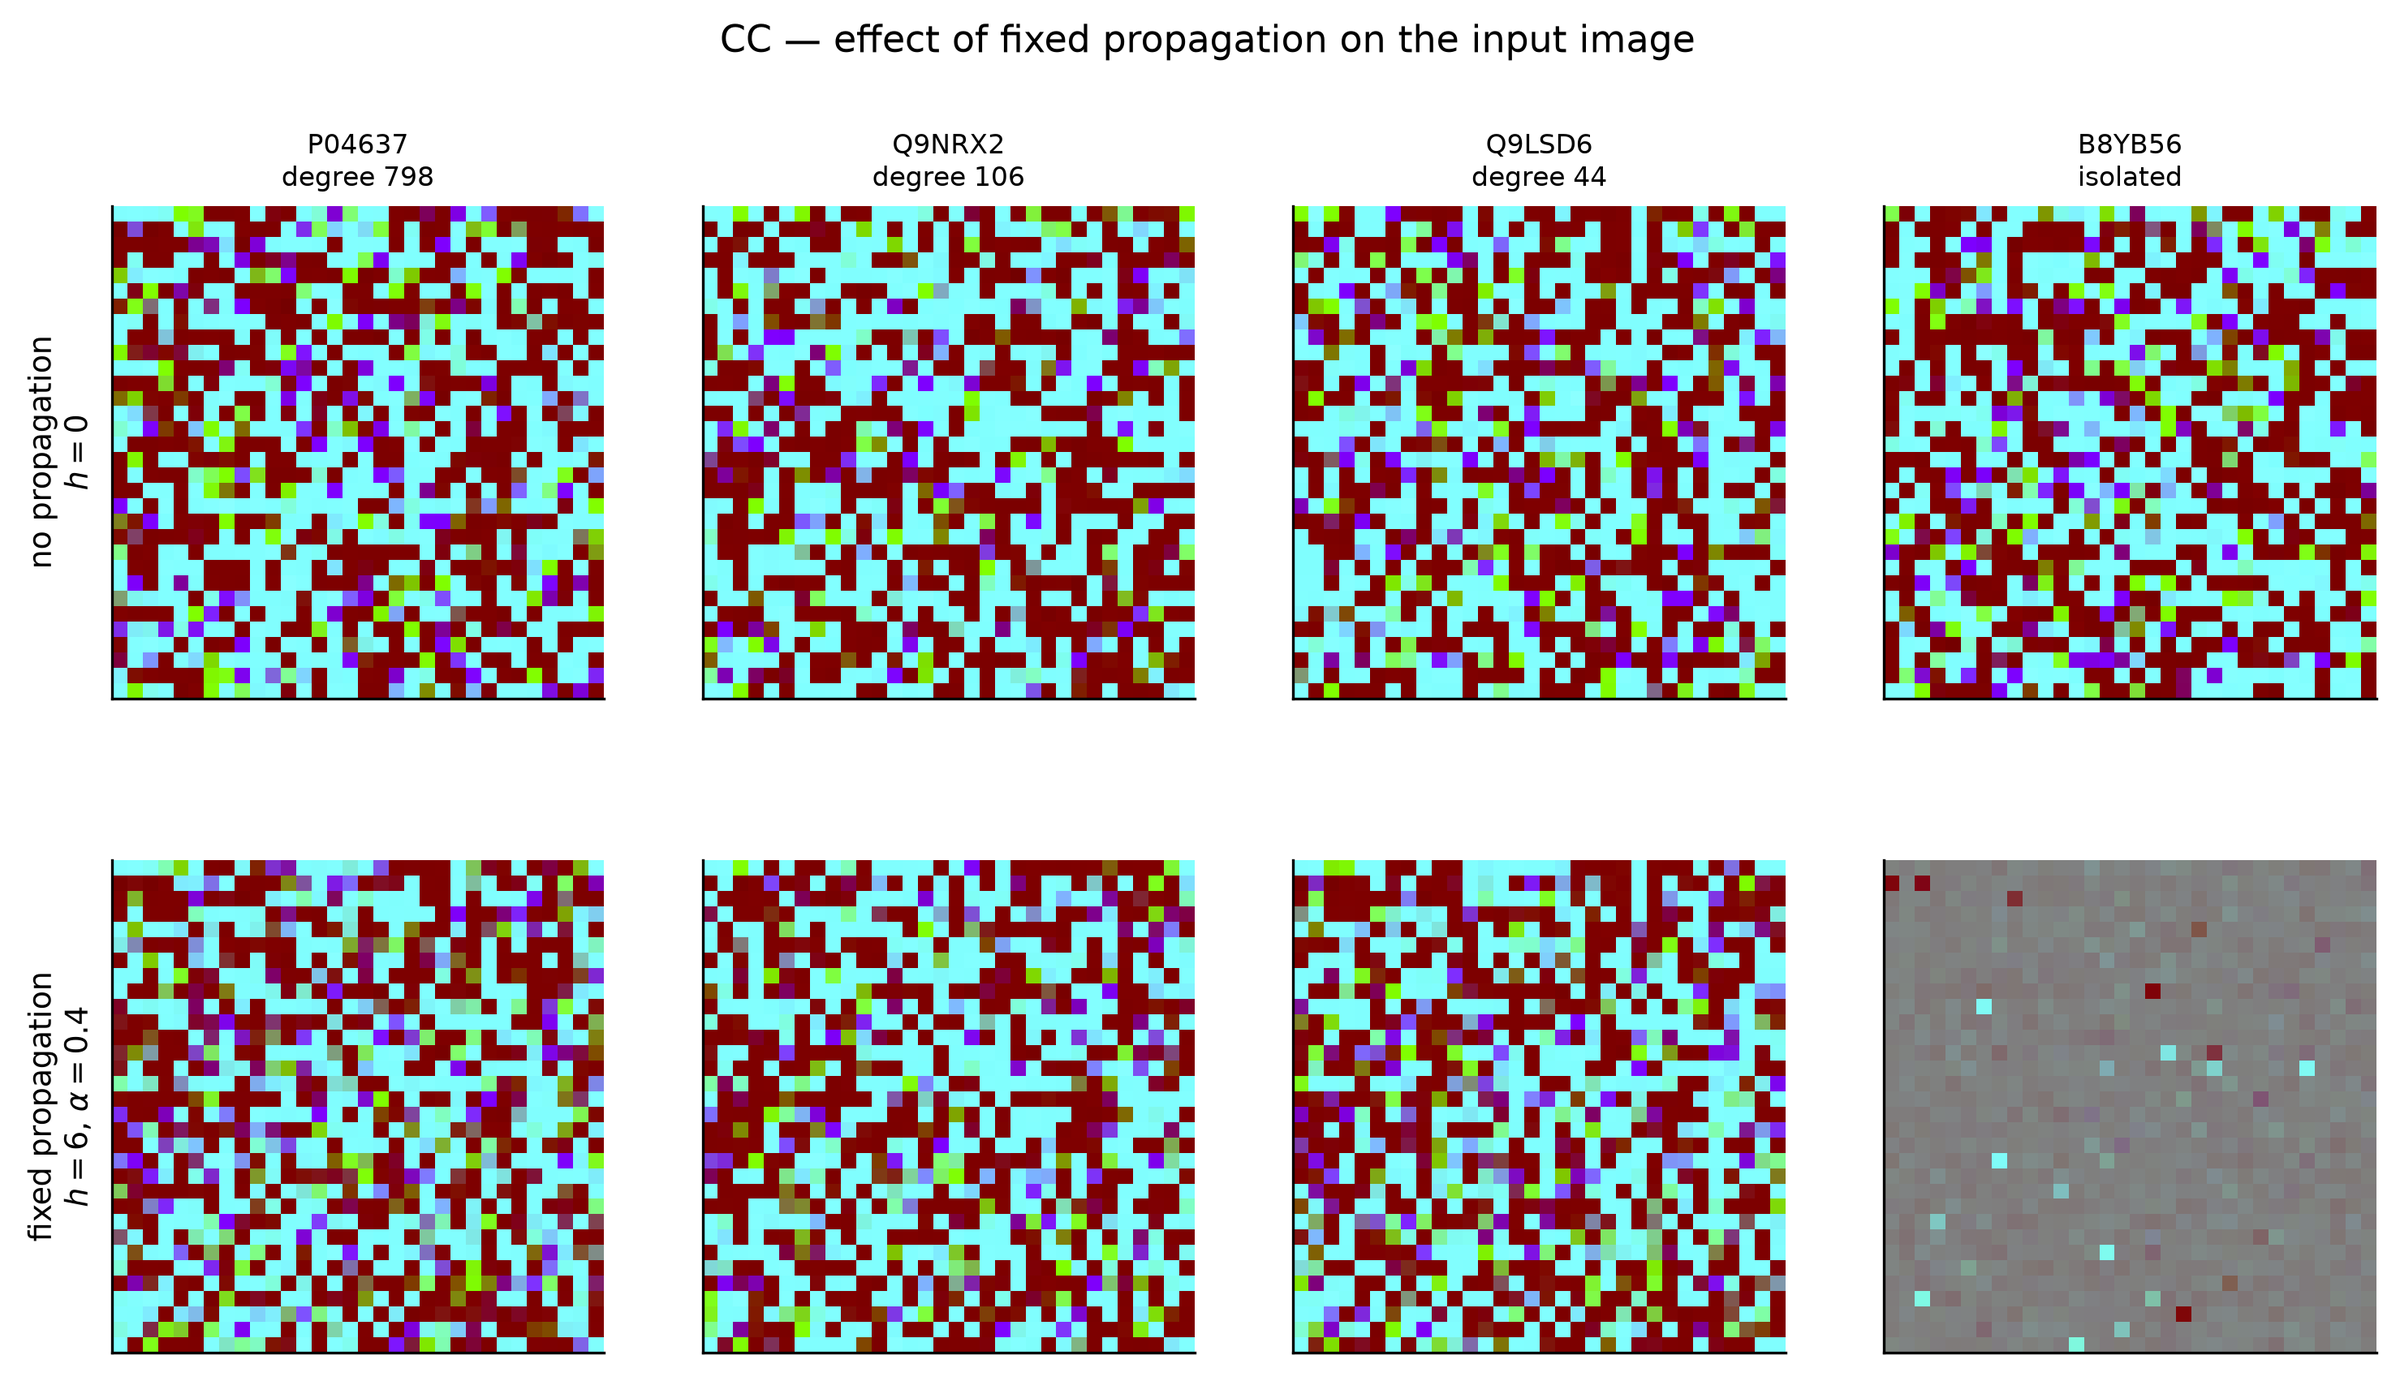
\includegraphics[width=896.7\px,height=514.5\px]{figures/fig_5_8.png}};
\node[tl] at (88,70) {\fmR\fz{16}{16}\color{inkii}\ls{2}\Ll{4 · Method}};
\node[tl] at (88,131) {\fdA\fz{54}{56.7}\color{ink}\ls{-1}\Ll{Propagation on four real proteins}};
\node<2-4>[tl] at (88,787.5) {\fmR\fz{15}{19.5}\color{muted}\Ll{Dissertation, Fig. 5.8 · CC, top {\fz{17.5}{21}$T = 0$}, bottom {\fz{17.5}{21}$T = 6,\ \alpha = 0.4$}}};
\node<3-4>[tl] at (1094.7,232) {\fbR\fz{26}{35.1}\color{ink}\Ll{Connected proteins keep their\\structure and absorb their\\neighbourhood}};
\node<4>[tl] at (1094.7,353.3) {\fbR\fz{26}{35.1}\color{ink}\Ll{An isolated protein becomes\\{\fz{29.2}{35}$\alpha^{T} \mathbf{H}^{(0)}$}: same direction,\\smaller scale}};
\node<4>[tl] at (1094.7,474.6) {\fbR\fz{26}{35.1}\color{ink}\Ll{So degree-zero gains cannot come\\from neighbourhood information}};
\node[tr] at (1512,876) {\fmR\fz{16}{16}\color{muted}25 / 45};
\end{tikzpicture}
\note{The rescaling is a structural property of the operator, not a tuned setting. 

The learned route adds self-loops and never mixes an isolated node with others.}
\end{frame}

\begin{frame}[plain]
\begin{tikzpicture}[deck]
\node<1>[box] at (0,0) {\includegraphics[page=3,width=1600\px]{build/layers}};
\node<2>[box] at (0,0) {\includegraphics[page=70,width=1600\px]{build/layers}};
\node<3>[box] at (0,0) {\includegraphics[page=82,width=1600\px]{build/layers}};
\node<4>[box] at (0,0) {\includegraphics[page=83,width=1600\px]{build/layers}};
\node<5>[box] at (0,0) {\includegraphics[page=84,width=1600\px]{build/layers}};
\node[tl] at (88,70) {\fmR\fz{16}{16}\color{inkii}\ls{2}\Ll{4 · Method}};
\node[tl] at (88,131) {\fdA\fz{54}{56.7}\color{ink}\ls{-1}\Ll{Learned propagation: GCN and GAT}};
\node<2-5>[tl] at (124,236) {\fbR\fz{30}{40.5}\color{ink}\Ll{GCN: symmetric normalization of\\{\fz{33.7}{40.4}$W + I$}, then a trained transform}};
\node<3-5>[tl] at (124,339) {\fbR\fz{30}{40.5}\color{ink}\Ll{GAT: attention over neighbours, 4 heads,\\edge score as attribute}};
\node<4-5>[tl] at (124,442) {\fbR\fz{30}{40.5}\color{ink}\Ll{2 layers, width 1024, output {\fz{33.7}{40.4}$\mathbf{g} \in \mathbb{R}^{1024}$}\\for the head}};
\node<5>[tl] at (124,545) {\fbR\fz{30}{40.5}\color{ink}\Ll{Full-graph forward on every step: about\\289 propagations per epoch}};
\node<2-5>[tl] at (694.7,220) {\fmR\fz{16}{16}\color{inkii}\Ll{GCN}};
\node<2-5>[tl] at (694.7,268.1) {\fbR\fz{28}{33.6}\color{ink}\Ll{{\fz{31.4}{37.7}$\displaystyle \mathbf{H}^{(\ell+1)} = \phi\!\left( \tilde{D}^{-1/2}\,\tilde{W}\,\tilde{D}^{-1/2}\,\mathbf{H}^{(\ell)}\,\Theta^{(\ell)} \right), \quad \tilde{W} = W + I$}}};
\node<3-5>[tl] at (694.7,336.5) {\fmR\fz{16}{16}\color{inkii}\Ll{GAT}};
\node<3-5>[tl] at (694.7,376.3) {\fbR\fz{28}{33.6}\color{ink}\Ll{{\fz{31.4}{37.7}$\displaystyle e_{ij} = \operatorname{LeakyReLU}\!\left( \mathbf{q}^{\top} \left[\, \Theta \mathbf{h}_i \,\|\, \Theta \mathbf{h}_j \,\|\, \Theta_e\, w_{ij} \,\right] \right)$}}};
\node<3-5>[tl] at (694.7,446.6) {\fbR\fz{28}{33.6}\color{ink}\Ll{{\fz{31.4}{37.7}$\displaystyle a_{ij} = \frac{\exp(e_{ij})}{\sum_{k \in \mathcal{N}(i) \cup \{i\}} \exp(e_{ik})}$}}};
\node<5>[tl] at (694.7,539.4) {\fbR\fz{22}{26.4}\color{inkii}\Ll{fixed}};
\node<5>[tl] at (862.7,570.4) {\fbR\fz{20}{27}\color{inkii}\Ll{computed once}};
\node<5>[tl] at (694.7,609.4) {\fbR\fz{22}{26.4}\color{inkii}\Ll{learned}};
\node<5>[tl] at (862.7,640.4) {\fbR\fz{20}{27}\color{inkii}\Ll{recomputed every optimization step}};
\node[tr] at (1512,876) {\fmR\fz{16}{16}\color{muted}26 / 45};
\end{tikzpicture}
\note{The GCN takes the STRING confidence as an edge weight; the GAT re-estimates it. 

Exact propagation with a mini-batch loss forces a full-graph pass for every batch, which is where the cost comes from.}
\end{frame}

\begin{frame}[plain]
\begin{tikzpicture}[deck]
\node<1>[box] at (0,0) {\includegraphics[page=3,width=1600\px]{build/layers}};
\node<2>[box] at (0,0) {\includegraphics[page=85,width=1600\px]{build/layers}};
\node<3>[box] at (0,0) {\includegraphics[page=86,width=1600\px]{build/layers}};
\node<4>[box] at (0,0) {\includegraphics[page=87,width=1600\px]{build/layers}};
\node<5>[box] at (0,0) {\includegraphics[page=88,width=1600\px]{build/layers}};
\node<3-5>[box] at (109,235) {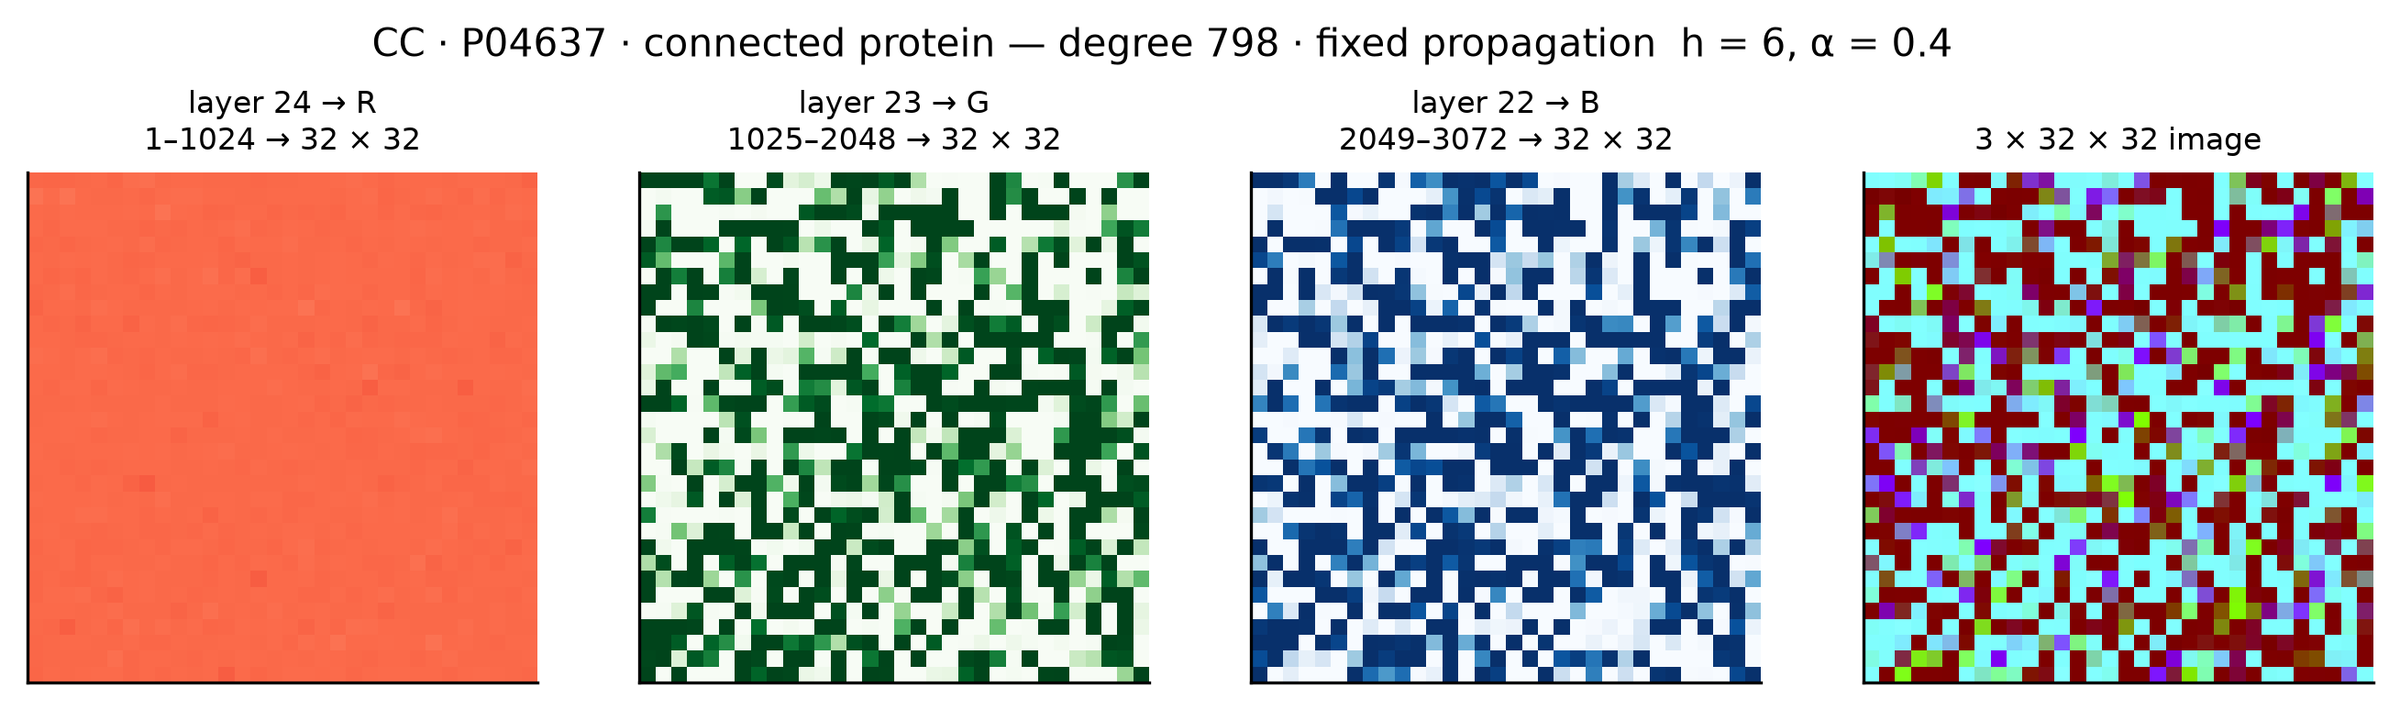
\includegraphics[width=1115.5\px,height=330\px]{figures/fig_5_9.png}};
\node[tl] at (88,70) {\fmR\fz{16}{16}\color{inkii}\ls{2}\Ll{4 · Method}};
\node[tl] at (88,131) {\fdA\fz{54}{56.7}\color{ink}\ls{-1}\Ll{Vector head and vision head}};
\node<3-5>[tl] at (88,603) {\fmR\fz{15}{19.5}\color{muted}\Ll{Dissertation, Fig. 5.9}};
\node<2-5>[tl] at (124,657.5) {\fbR\fz{26}{35.1}\color{ink}\Ll{Vector: MLP [1024, 512], batch norm, dropout 0.4}};
\node<4-5>[tl] at (856,657.5) {\fbR\fz{26}{35.1}\color{ink}\Ll{Backbones: ResNet-50 and ConvNeXt-Tiny (ImageNet),\\fully fine-tuned}};
\node<3-5>[tl] at (124,759.8) {\fbR\fz{26}{35.1}\color{ink}\Ll{Vision: {\fz{29.2}{35}$\sigma(\mathrm{clip}(z))$} split into three 32 × 32 channels, one\\per ProtT5 layer}};
\node<5>[tl] at (856,759.8) {\fbR\fz{26}{35.1}\color{ink}\Ll{Caution: pixel adjacency has no meaning here}};
\node[tr] at (1512,876) {\fmR\fz{16}{16}\color{muted}27 / 45};
\end{tikzpicture}
\note{The image is built inside the forward pass and never written to disk. 

Neighbouring pixels are neighbouring embedding coordinates only by storage order, a caveat that the results confirm.}
\end{frame}

\begin{frame}[plain]
\begin{tikzpicture}[deck]
\node<1-2>[box] at (0,0) {\includegraphics[page=3,width=1600\px]{build/layers}};
\node<3>[box] at (0,0) {\includegraphics[page=89,width=1600\px]{build/layers}};
\node<4>[box] at (0,0) {\includegraphics[page=90,width=1600\px]{build/layers}};
\node<5>[box] at (0,0) {\includegraphics[page=91,width=1600\px]{build/layers}};
\node[tl] at (88,70) {\fmR\fz{16}{16}\color{inkii}\ls{2}\Ll{4 · Method}};
\node[tl] at (88,131) {\fdA\fz{54}{56.7}\color{ink}\ls{-1}\Ll{Training objective: ProteinLoss}};
\node<2-5>[tl] at (88,251.7) {\fbR\fz{44}{52.8}\color{ink}\Ll{{\fz{49.4}{59.2}$\displaystyle \mathcal{L} = \mathcal{L}_{\text{ZLPR}} \cdot \bigl(1 - \mathrm{wF}_1^{\text{GO}}\bigr) \cdot \bigl(1 - \mathrm{wF}_1^{\text{prot}}\bigr)$}}};
\node<3-5>[tl] at (124,335) {\fbR\fz{30}{40.5}\color{ink}\Ll{ZLPR separates positive from negative\\terms at threshold zero}};
\node<4-5>[tl] at (124,438) {\fbR\fz{30}{40.5}\color{ink}\Ll{Two soft, IC-weighted {\fz{33.7}{40.4}$F_1$} factors: one\\across terms, one across proteins}};
\node<5>[tl] at (124,541) {\fbR\fz{30}{40.5}\color{ink}\Ll{Brings training closer to the\\evaluation criterion}};
\node[tr] at (1512,876) {\fmR\fz{16}{16}\color{muted}28 / 45};
\end{tikzpicture}
\note{Inherited from InterLabelGO+ through the group's sequence-only line. 

It beats binary cross-entropy by 5.47 pp on the first-generation mean, so every later run uses it.}
\end{frame}

\begin{frame}[plain]
\begin{tikzpicture}[deck]
\node<1>[box] at (0,0) {\includegraphics[page=3,width=1600\px]{build/layers}};
\node<2>[box] at (0,0) {\includegraphics[page=92,width=1600\px]{build/layers}};
\node<3>[box] at (0,0) {\includegraphics[page=93,width=1600\px]{build/layers}};
\node<4>[box] at (0,0) {\includegraphics[page=94,width=1600\px]{build/layers}};
\node<5>[box] at (0,0) {\includegraphics[page=95,width=1600\px]{build/layers}};
\node<6>[box] at (0,0) {\includegraphics[page=96,width=1600\px]{build/layers}};
\node<2-6>[box] at (109,235) {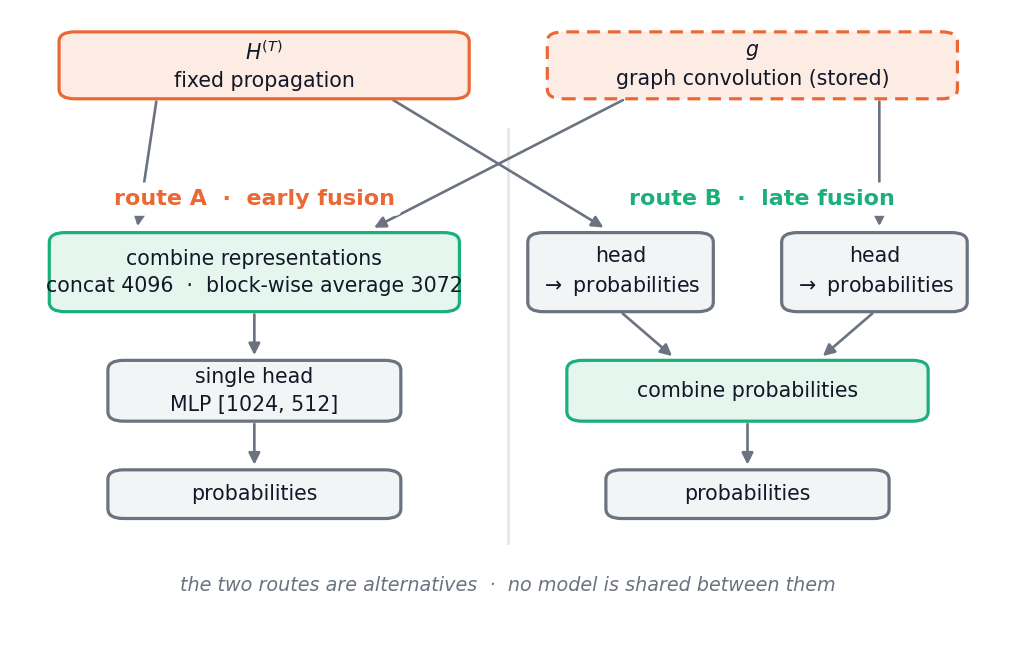
\includegraphics[width=654\px,height=417.1\px]{figures/fig_5_10.png}};
\node[tl] at (88,70) {\fmR\fz{16}{16}\color{inkii}\ls{2}\Ll{4 · Method}};
\node[tl] at (88,131) {\fdA\fz{54}{56.7}\color{ink}\ls{-1}\Ll{Combining the fixed and learned routes}};
\node<2-6>[tl] at (88,690.1) {\fmR\fz{15}{19.5}\color{muted}\Ll{Dissertation, Fig. 5.10}};
\node<3-6>[tl] at (852,232) {\fbR\fz{26}{35.1}\color{ink}\Ll{Early: join representations, train one head (concat 4096\\or block-wise add 3072)}};
\node<4-6>[tl] at (852,318.2) {\fbR\fz{26}{35.1}\color{ink}\Ll{Late: train each route, combine probabilities}};
\node<5-6>[tl] at (852,369.3) {\fbR\fz{26}{35.1}\color{ink}\Ll{Eleven late rules: linear {\fz{29.2}{35}$\gamma$}, max, min, IC sigmoid, degree\\sigmoid, master equation, five stacking meta-classifiers}};
\node<6>[tl] at (852,455.5) {\fbR\fz{26}{35.1}\color{ink}\Ll{Coefficients chosen on validation (71 configurations\\per ontology)}};
\node[tr] at (1512,876) {\fmR\fz{16}{16}\color{muted}29 / 45};
\end{tikzpicture}
\note{The two routes are alternatives, no model is shared. 

Early fusion lets one head learn how to weigh the sources; late fusion leaves each route to its own optimization and needs no training to combine.}
\end{frame}

\section{5 · Results}
\begin{frame}[plain]
\begin{tikzpicture}[deck]
\node<1>[box] at (0,0) {\includegraphics[page=3,width=1600\px]{build/layers}};
\node<2>[box] at (0,0) {\includegraphics[page=7,width=1600\px]{build/layers}};
\node<3>[box] at (0,0) {\includegraphics[page=97,width=1600\px]{build/layers}};
\node<4>[box] at (0,0) {\includegraphics[page=98,width=1600\px]{build/layers}};
\node[tl] at (88,70) {\fmR\fz{16}{16}\color{inkii}\ls{2}\Ll{5 · Results}};
\node[tl] at (88,131) {\fdA\fz{54}{56.7}\color{ink}\ls{-1}\Ll{170 runs, one funnel}};
\node<2-4>[tl] at (124,236) {\fbR\fz{30}{40.5}\color{ink}\Ll{170 runs, about 136.3 GPU-\\hours (147 on an RTX A5500)}};
\node<3-4>[tl] at (612,236) {\fbR\fz{30}{40.5}\color{ink}\Ll{Each stage picks its winner on\\validation and hands it on}};
\node<4>[tl] at (1100,236) {\fbR\fz{30}{40.5}\color{ink}\Ll{Test read once, at the end}};
\node[tr] at (1512,876) {\fmR\fz{16}{16}\color{muted}30 / 45};
\end{tikzpicture}
\note{The selection never touches the test partition. Every reported test number is a single evaluation of a frozen configuration. 

Two stations are not pure validation picks: max deduplication rests on an analytic argument (all 170 runs use it; the sum figures come from the earlier campaign), and ConvNeXt-Tiny is carried forward on a 0.57 pp margin plus the VISAPP campaign.}
\end{frame}

\begin{frame}[plain]
\begin{tikzpicture}[deck]
\node<1>[box] at (0,0) {\includegraphics[page=99,width=1600\px]{build/layers}};
\node<2>[box] at (0,0) {\includegraphics[page=100,width=1600\px]{build/layers}};
\node<3>[box] at (0,0) {\includegraphics[page=101,width=1600\px]{build/layers}};
\node<4>[box] at (0,0) {\includegraphics[page=102,width=1600\px]{build/layers}};
\node<5>[box] at (0,0) {\includegraphics[page=103,width=1600\px]{build/layers}};
\node[tl] at (88,70) {\fmR\fz{16}{16}\color{inkii}\ls{2}\Ll{5 · Results}};
\node[tl] at (88,131) {\fdA\fz{54}{56.7}\color{ink}\ls{-1}\Ll{Generation 1 settles three choices}};
\node<2-5>[tl] at (124,232) {\fbR\fz{26}{35.1}\color{ink}\Ll{Naive term-frequency baseline: 43.56\\mean wF\textsubscript{max}}};
\node<3-5>[tl] at (124,318.2) {\fbR\fz{26}{35.1}\color{ink}\Ll{ProteinLoss beats binary cross-entropy: +5.47\\pp mean (+8.87 in MF)}};
\node<4-5>[tl] at (124,404.4) {\fbR\fz{26}{35.1}\color{ink}\Ll{MLP on the raw profile wins: 44.51; best 1-D\\CNN 41.16}};
\node<5>[tl] at (124,490.6) {\fbR\fz{26}{35.1}\color{ink}\Ll{Vision backbones: 36.99 to 37.62}};
\node[tr] at (1512,876) {\fmR\fz{16}{16}\color{muted}31 / 45};
\end{tikzpicture}
\note{Topology alone barely clears a predictor that looks at nothing: 0.95 pp on the mean, and below it in BP. 

The vector route wins, and ConvNeXt-Tiny is carried forward on a 0.57 pp margin plus the earlier VISAPP campaign.}
\end{frame}

\begin{frame}[plain]
\begin{tikzpicture}[deck]
\node<1>[box] at (0,0) {\includegraphics[page=3,width=1600\px]{build/layers}};
\node<2>[box] at (0,0) {\includegraphics[page=104,width=1600\px]{build/layers}};
\node<3>[box] at (0,0) {\includegraphics[page=105,width=1600\px]{build/layers}};
\node<4>[box] at (0,0) {\includegraphics[page=106,width=1600\px]{build/layers}};
\node<2-4>[box] at (159.6,235) {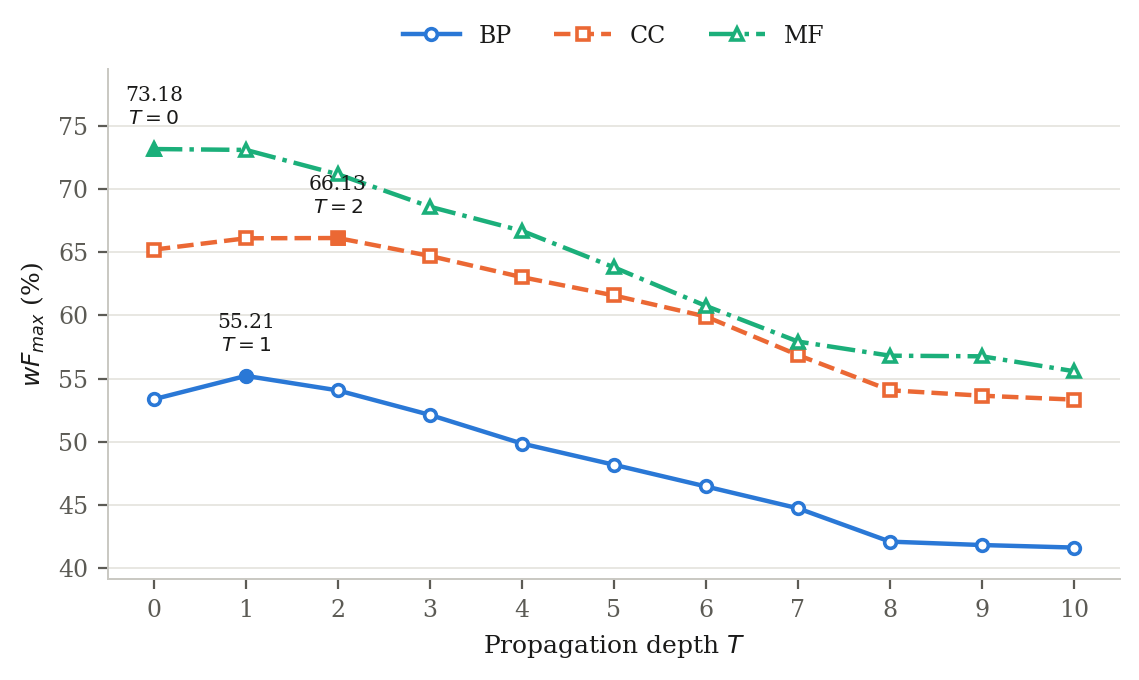
\includegraphics[width=552.8\px,height=330\px]{figures/fig_6_1.png}};
\node<3-4>[box] at (887.6,235) {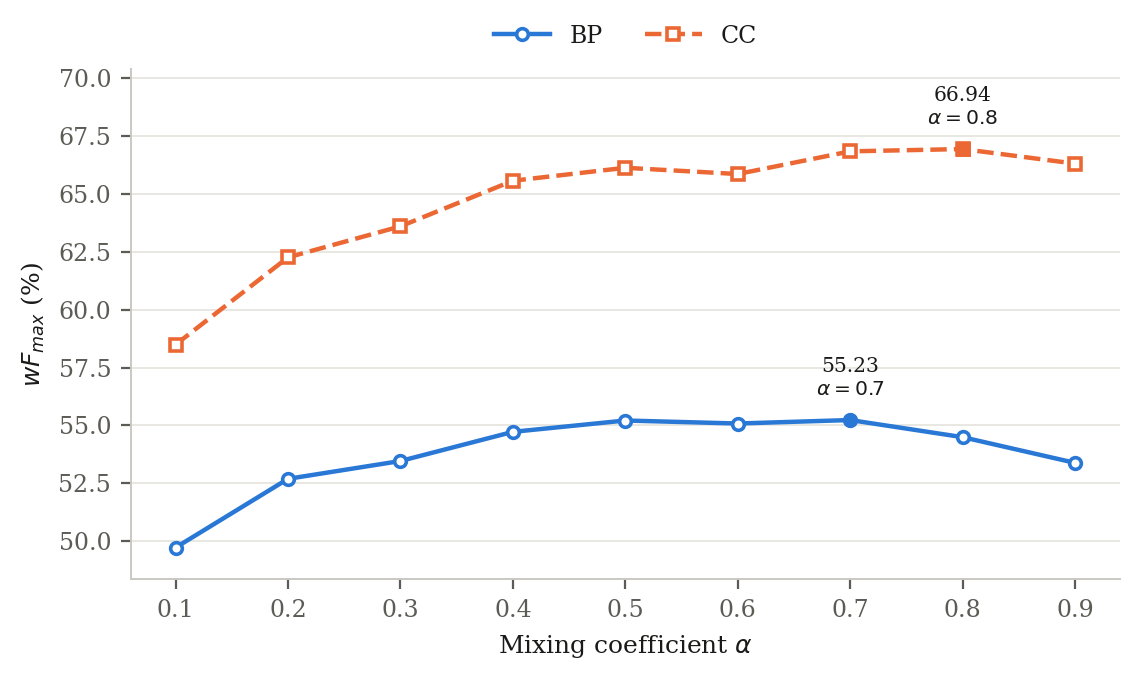
\includegraphics[width=552.8\px,height=330\px]{figures/fig_6_2.png}};
\node[tl] at (88,70) {\fmR\fz{16}{16}\color{inkii}\ls{2}\Ll{5 · Results}};
\node[tl] at (88,131) {\fdA\fz{54}{56.7}\color{ink}\ls{-1}\Ll{One or two hops, high retention}};
\node<2-4>[tl] at (88,603) {\fmR\fz{15}{19.5}\color{muted}\Ll{Dissertation, Fig. 6.1 · vector head, depth, validation}};
\node<3-4>[tl] at (816,603) {\fmR\fz{15}{19.5}\color{muted}\Ll{Dissertation, Fig. 6.2 · vector head, retention, validation}};
\node<2-4>[tl] at (124,655.5) {\fbR\fz{26}{35.1}\color{ink}\Ll{Peak depth: {\fz{29.2}{35}$T = 1$} BP, {\fz{29.2}{35}$T = 2$} CC, {\fz{29.2}{35}$T = 0$} MF}};
\node<3-4>[tl] at (852,655.5) {\fbR\fz{26}{35.1}\color{ink}\Ll{Best retention: {\fz{29.2}{35}$\alpha = 0.7$} BP, {\fz{29.2}{35}$\alpha = 0.8$} CC}};
\node<2-4>[tl] at (124,741.2) {\fbR\fz{26}{35.1}\color{ink}\Ll{Beyond the peak, performance falls 12.80 to 17.60 pp\\by {\fz{29.2}{35}$T = 10$}}};
\node<4>[tl] at (852,741.2) {\fbR\fz{26}{35.1}\color{ink}\Ll{The graph corrects the protein's own representation; it\\does not replace it}};
\node[tr] at (1512,876) {\fmR\fz{16}{16}\color{muted}32 / 45};
\end{tikzpicture}
\note{In MF no amount of propagation helps; the best configuration switches the graph off. 

In CC everything below $\alpha$ = 0.4 is worse than everything above it; in BP the single exception is $\alpha$ = 0.9.}
\end{frame}

\begin{frame}[plain]
\begin{tikzpicture}[deck]
\node<1>[box] at (0,0) {\includegraphics[page=3,width=1600\px]{build/layers}};
\node<2>[box] at (0,0) {\includegraphics[page=107,width=1600\px]{build/layers}};
\node<3>[box] at (0,0) {\includegraphics[page=108,width=1600\px]{build/layers}};
\node<4>[box] at (0,0) {\includegraphics[page=109,width=1600\px]{build/layers}};
\node<2-4>[box] at (159.6,235) {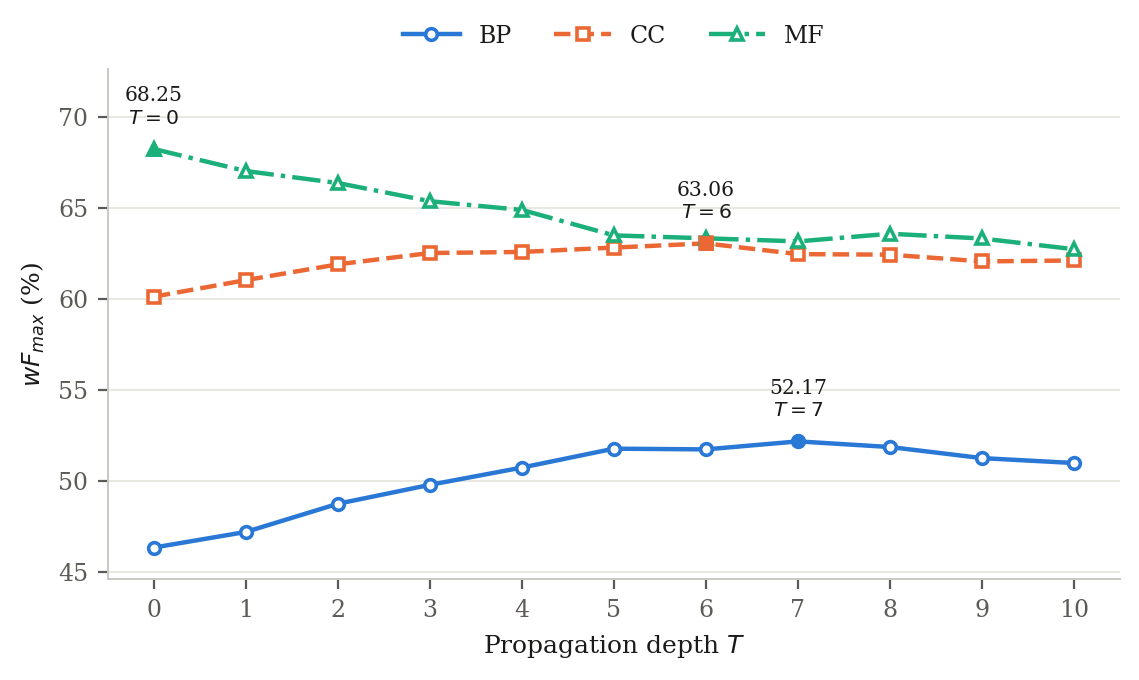
\includegraphics[width=552.8\px,height=330\px]{figures/fig_6_3.png}};
\node<3-4>[box] at (887.6,235) {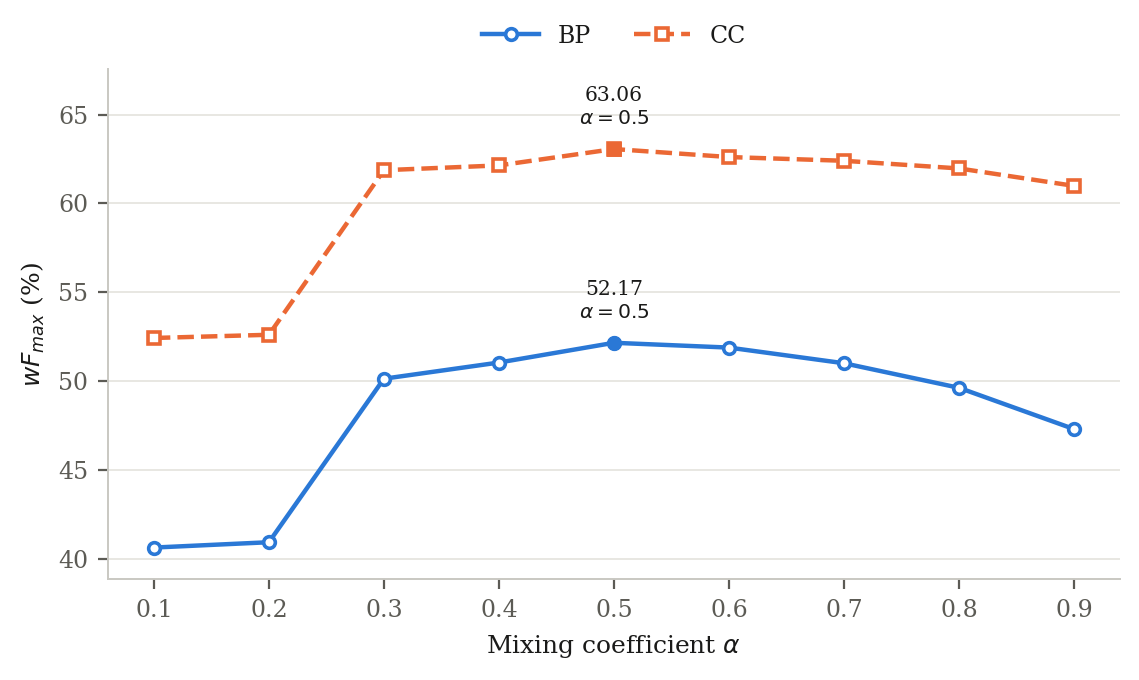
\includegraphics[width=552.8\px,height=330\px]{figures/fig_6_4.png}};
\node[tl] at (88,70) {\fmR\fz{16}{16}\color{inkii}\ls{2}\Ll{5 · Results}};
\node[tl] at (88,131) {\fdA\fz{54}{56.7}\color{ink}\ls{-1}\Ll{The vision head wants deep propagation}};
\node<2-4>[tl] at (88,603) {\fmR\fz{15}{19.5}\color{muted}\Ll{Dissertation, Fig. 6.3 · vision head, depth, validation}};
\node<3-4>[tl] at (816,603) {\fmR\fz{15}{19.5}\color{muted}\Ll{Dissertation, Fig. 6.4 · vision head, retention, validation}};
\node<2-4>[tl] at (124,655.5) {\fbR\fz{26}{35.1}\color{ink}\Ll{Peak depth: {\fz{29.2}{35}$T = 7$} BP, {\fz{29.2}{35}$T = 6$} CC, {\fz{29.2}{35}$T = 0$} MF; a plateau,\\not a peak}};
\node<3-4>[tl] at (852,655.5) {\fbR\fz{26}{35.1}\color{ink}\Ll{Collapse at {\fz{29.2}{35}$\alpha \le 0.2$}: isolated nodes shrink as {\fz{29.2}{35}$\alpha^{T}$} ({\fz{29.2}{35}$10^{-7}$}\\at {\fz{29.2}{35}$T = 7$})}};
\node<2-4>[tl] at (124,758.8) {\fbR\fz{26}{35.1}\color{ink}\Ll{Gains over {\fz{29.2}{35}$T = 0$}: +5.84 BP, +2.93 CC (vector head:\\+1.85, +0.92)}};
\node<4>[tl] at (852,758.8) {\fbR\fz{26}{35.1}\color{ink}\Ll{Its best BP value, 52.17, is still below the vector head's\\graph-free 53.36}};
\node[tr] at (1512,876) {\fmR\fz{16}{16}\color{muted}33 / 45};
\end{tikzpicture}
\note{The vision head extracts less from the node itself, so dilution costs it less and the neighbourhood average helps more. 

MF peaks at T = 0 in both heads, the strongest form of that observation.}
\end{frame}

\begin{frame}[plain]
\begin{tikzpicture}[deck]
\node<1>[box] at (0,0) {\includegraphics[page=110,width=1600\px]{build/layers}};
\node<2>[box] at (0,0) {\includegraphics[page=111,width=1600\px]{build/layers}};
\node<3>[box] at (0,0) {\includegraphics[page=112,width=1600\px]{build/layers}};
\node<4>[box] at (0,0) {\includegraphics[page=113,width=1600\px]{build/layers}};
\node<5>[box] at (0,0) {\includegraphics[page=114,width=1600\px]{build/layers}};
\node[tl] at (88,70) {\fmR\fz{16}{16}\color{inkii}\ls{2}\Ll{5 · Results}};
\node[tl] at (88,131) {\fdA\fz{54}{56.7}\color{ink}\ls{-1}\Ll{Learning the aggregation does not pay}};
\node<2-5>[tl] at (124,232) {\fbR\fz{26}{35.1}\color{ink}\Ll{GCN beats GAT in all 6 pairs (3.88 to 9.31 pp),\\and in 30 of 30 fusion pairs}};
\node<3-5>[tl] at (124,318.2) {\fbR\fz{26}{35.1}\color{ink}\Ll{Fixed 65.12 vs GCN 63.32 mean wF\textsubscript{max}}};
\node<4-5>[tl] at (124,369.3) {\fbR\fz{26}{35.1}\color{ink}\Ll{GCN ahead in BP by 0.55 (a tie); behind in CC\\by 0.59 and MF by 5.35}};
\node<5>[tl] at (124,455.5) {\fbR\fz{26}{35.1}\color{ink}\Ll{Deduplication: max never loses beyond noise;\\GAT gains most (+3.83 vision)}};
\node[tr] at (1512,876) {\fmR\fz{16}{16}\color{muted}34 / 45};
\end{tikzpicture}
\note{Attention does not recover a better weighting than the STRING score it was handed. 

A plausible reason: the loss is masked to training nodes, so attention parameters see gradient only through a two-hop receptive field.}
\end{frame}

\begin{frame}[plain]
\begin{tikzpicture}[deck]
\node<1>[box] at (0,0) {\includegraphics[page=115,width=1600\px]{build/layers}};
\node<2>[box] at (0,0) {\includegraphics[page=116,width=1600\px]{build/layers}};
\node<3>[box] at (0,0) {\includegraphics[page=117,width=1600\px]{build/layers}};
\node<4>[box] at (0,0) {\includegraphics[page=118,width=1600\px]{build/layers}};
\node<5>[box] at (0,0) {\includegraphics[page=119,width=1600\px]{build/layers}};
\node[tl] at (88,70) {\fmR\fz{16}{16}\color{inkii}\ls{2}\Ll{5 · Results}};
\node[tl] at (88,131) {\fdA\fz{54}{56.7}\color{ink}\ls{-1}\Ll{Fusion helps; combining predictions helps more}};
\node<2-5>[tl] at (124,232) {\fbR\fz{26}{35.1}\color{ink}\Ll{Early, one configuration (add, GCN, vector):\\65.80, +0.68 over fixed alone}};
\node<3-5>[tl] at (124,318.2) {\fbR\fz{26}{35.1}\color{ink}\Ll{Late, linear {\fz{29.2}{35}$\gamma$} (0.50 BP, 0.55 CC and MF):\\67.06, best in every ontology}};
\node<4-5>[tl] at (124,404.4) {\fbR\fz{26}{35.1}\color{ink}\Ll{Gains over the better component: +2.18 BP,\\+1.85 CC, +1.26 MF}};
\node<5>[tl] at (124,490.6) {\fbR\fz{26}{35.1}\color{ink}\Ll{Stacking importances: the two probabilities\\carry almost all the weight}};
\node[tr] at (1512,876) {\fmR\fz{16}{16}\color{muted}35 / 45};
\end{tikzpicture}
\note{A single scalar beats every elaborate rule, including gradient boosting. The auxiliary features do not predict which route is right, and the conditional rules converged to the flattest sigmoid in the grid. 

The ensemble fits one extra parameter on validation.}
\end{frame}

\begin{frame}[plain]
\begin{tikzpicture}[deck]
\node<1>[box] at (0,0) {\includegraphics[page=120,width=1600\px]{build/layers}};
\node<2>[box] at (0,0) {\includegraphics[page=121,width=1600\px]{build/layers}};
\node<3>[box] at (0,0) {\includegraphics[page=122,width=1600\px]{build/layers}};
\node<4>[box] at (0,0) {\includegraphics[page=123,width=1600\px]{build/layers}};
\node[tl] at (88,70) {\fmR\fz{16}{16}\color{inkii}\ls{2}\Ll{5 · Results}};
\node[tl] at (88,131) {\fdA\fz{54}{56.7}\color{ink}\ls{-1}\Ll{Vector head wins 12 of 12}};
\node<3-4>[tl] at (1094.7,232) {\fbR\fz{26}{35.1}\color{ink}\Ll{Margin on the mean: +6.62,\\+3.96, +2.69, +3.35 pp across the\\four stages}};
\node<3-4>[tl] at (1094.7,353.3) {\fbR\fz{26}{35.1}\color{ink}\Ll{No trend toward zero}};
\node<4>[tl] at (1094.7,404.4) {\fbR\fz{26}{35.1}\color{ink}\Ll{Neither image has the locality a\\convolution assumes}};
\node[tr] at (1512,876) {\fmR\fz{16}{16}\color{muted}36 / 45};
\end{tikzpicture}
\note{Generation 1 images index arbitrary training proteins; generation 2 images reshape embedding coordinates. 

Three independent pieces of evidence agree: pooling order, the 1-D CNN failure and this table.}
\end{frame}

\begin{frame}[plain]
\begin{tikzpicture}[deck]
\node<1>[box] at (0,0) {\includegraphics[page=124,width=1600\px]{build/layers}};
\node<2>[box] at (0,0) {\includegraphics[page=125,width=1600\px]{build/layers}};
\node<3>[box] at (0,0) {\includegraphics[page=126,width=1600\px]{build/layers}};
\node<4>[box] at (0,0) {\includegraphics[page=127,width=1600\px]{build/layers}};
\node<5>[box] at (0,0) {\includegraphics[page=128,width=1600\px]{build/layers}};
\node[tl] at (88,70) {\fmR\fz{16}{16}\color{inkii}\ls{2}\Ll{5 · Results}};
\node[tl] at (88,131) {\fdA\fz{54}{56.7}\color{ink}\ls{-1}\Ll{Where the gains come from}};
\node<4-5>[tl] at (124,688) {\fbR\fz{26}{35.1}\color{ink}\Ll{Mean validation wF\textsubscript{max}: Naive 43.56 $\rightarrow$ Generation 1 44.51 $\rightarrow$ ProtT5 alone 63.92 $\rightarrow$ Fixed 65.12 $\rightarrow$ Early 65.84 $\rightarrow$\\Late 67.06}};
\node<5>[tl] at (124,774.2) {\fbR\fz{26}{35.1}\color{ink}\Ll{Most of the jump is the language model; the graph adds the rest}};
\node[tr] at (1512,876) {\fmR\fz{16}{16}\color{muted}37 / 45};
\end{tikzpicture}
\note{This is the whole dissertation on one axis. The protein language model explains most of the distance, and the graph contributes a consistent remainder in BP and CC. 

Each value is a mean of per-ontology champions on validation; the learned GNN alone, 63.32, sits below the ProtT5 control because of MF, so it is not a step of the staircase.}
\end{frame}

\begin{frame}[plain]
\hypertarget<1>{s38.1}{}
\hypertarget<2>{s38.2}{}
\hypertarget<3>{s38.3}{}
\hypertarget<4>{s38.4}{}
\hypertarget<5>{s38.5}{}
\hypertarget<6>{s38.6}{}
\hypertarget<7>{s38.7}{}
\begin{tikzpicture}[deck]
\node<1>[box] at (0,0) {\includegraphics[page=129,width=1600\px]{build/layers}};
\node<2>[box] at (0,0) {\includegraphics[page=130,width=1600\px]{build/layers}};
\node<3>[box] at (0,0) {\includegraphics[page=131,width=1600\px]{build/layers}};
\node<4>[box] at (0,0) {\includegraphics[page=132,width=1600\px]{build/layers}};
\node<5>[box] at (0,0) {\includegraphics[page=133,width=1600\px]{build/layers}};
\node<6>[box] at (0,0) {\includegraphics[page=134,width=1600\px]{build/layers}};
\node<7>[box] at (0,0) {\includegraphics[page=135,width=1600\px]{build/layers}};
\node<5>[box] at (787.5,208) {\hot{58.1}{42}{s38.5}};
\node<5>[box] at (844.1,208) {\hot{59.4}{42}{s38.6}};
\node<5>[box] at (902,208) {\hot{61.5}{42}{s38.7}};
\node<5>[box] at (1049.1,206) {\hot{227}{46}{s38x.4}};
\node<6>[box] at (787.5,208) {\hot{58.1}{42}{s38.5}};
\node<6>[box] at (844.1,208) {\hot{59.4}{42}{s38.6}};
\node<6>[box] at (902,208) {\hot{61.5}{42}{s38.7}};
\node<6>[box] at (1049.1,206) {\hot{227}{46}{s38x.10}};
\node<7>[box] at (787.5,208) {\hot{58.1}{42}{s38.5}};
\node<7>[box] at (844.1,208) {\hot{59.4}{42}{s38.6}};
\node<7>[box] at (902,208) {\hot{61.5}{42}{s38.7}};
\node<7>[box] at (1049.1,206) {\hot{227}{46}{s38x.16}};
\node[tl] at (88,70) {\fmR\fz{16}{16}\color{inkii}\ls{2}\Ll{5 · Results}};
\node[tl] at (88,131) {\fdA\fz{54}{56.7}\color{ink}\ls{-1}\Ll{Test set: NEXUS-GO vs five methods}};
\node<2-7>[tl] at (124,232) {\fbR\fz{26}{35.1}\color{ink}\Ll{NEXUS-GO/Late best in every column of the\\three tables, except AuPRC in MF}};
\node<3-7>[tl] at (124,318.2) {\fbR\fz{26}{35.1}\color{ink}\Ll{wF\textsubscript{max} margin over the strongest baseline:\\+9.77 BP, +8.67 CC, +4.93 MF}};
\node<4-7>[tl] at (124,404.4) {\fbR\fz{26}{35.1}\color{ink}\Ll{S\textsubscript{min}: 17.12 vs 20.11 (BP), 8.22 vs 9.67 (CC), 5.14\\vs 5.67 (MF)}};
\node<5-7>[tl] at (124,490.6) {\fbR\fz{26}{35.1}\color{ink}\Ll{The ProtT5 baseline alone already beats every\\literature method on wF\textsubscript{max}}};
\node[tr] at (1512,876) {\fmR\fz{16}{16}\color{muted}38 / 45};
\end{tikzpicture}
\note{Every baseline was retrained on the same corpus and scored with the same code. 

Three of them lose their multi-network mechanism on a single aggregated graph, so the ordering describes these adapted configurations, not the original papers.}
\end{frame}

\begin{frame}[plain]
\begin{tikzpicture}[deck]
\node<1>[box] at (0,0) {\includegraphics[page=136,width=1600\px]{build/layers}};
\node<2>[box] at (0,0) {\includegraphics[page=137,width=1600\px]{build/layers}};
\node<3>[box] at (0,0) {\includegraphics[page=138,width=1600\px]{build/layers}};
\node[tl] at (88,70) {\fmR\fz{16}{16}\color{inkii}\ls{2}\Ll{5 · Results}};
\node[tl] at (88,131) {\fdA\fz{54}{56.7}\color{ink}\ls{-1}\Ll{Every protein gets a prediction}};
\node<2-3>[tl] at (124,236) {\fbR\fz{30}{40.5}\color{ink}\Ll{NEXUS-GO: 100\% of the test partition in\\BP, CC, MF}};
\node<3>[tl] at (124,339) {\fbR\fz{30}{40.5}\color{ink}\Ll{DeepGraphGO and SEGT-GO: 95.1–\\96.3\% (homology search)}};
\node<3>[tl] at (124,442) {\fbR\fz{30}{40.5}\color{ink}\Ll{Mashup, MELISSA, deepNF: 63.6–68.7\%\\(network members only)}};
\node[tr] at (1512,876) {\fmR\fz{16}{16}\color{muted}39 / 45};
\end{tikzpicture}
\note{Missing proteins count as misses in the comparison, so part of the distance to the network-only methods is reach, not ranking quality. 

The proteins they cannot reach are exactly the band where sequence-aware routes score highest.}
\end{frame}

\begin{frame}[plain]
\begin{tikzpicture}[deck]
\node<1>[box] at (0,0) {\includegraphics[page=3,width=1600\px]{build/layers}};
\node<2>[box] at (0,0) {\includegraphics[page=139,width=1600\px]{build/layers}};
\node<3>[box] at (0,0) {\includegraphics[page=140,width=1600\px]{build/layers}};
\node<4>[box] at (0,0) {\includegraphics[page=141,width=1600\px]{build/layers}};
\node<5>[box] at (0,0) {\includegraphics[page=142,width=1600\px]{build/layers}};
\node<2-5>[box] at (109,235) {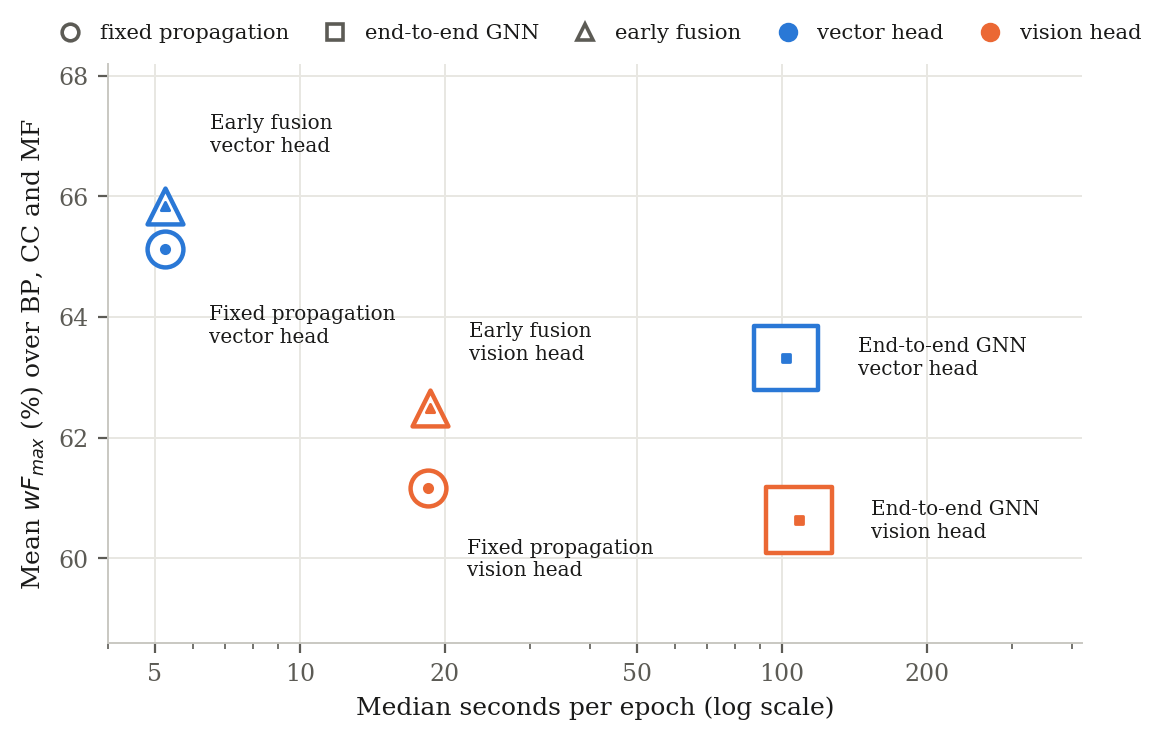
\includegraphics[width=654\px,height=415.4\px]{figures/fig_6_5.png}};
\node[tl] at (88,70) {\fmR\fz{16}{16}\color{inkii}\ls{2}\Ll{5 · Results}};
\node[tl] at (88,131) {\fdA\fz{54}{56.7}\color{ink}\ls{-1}\Ll{A thirteenth of the time per epoch}};
\node<2-5>[tl] at (88,688.4) {\fmR\fz{15}{19.5}\color{muted}\Ll{Dissertation, Fig. 6.5}};
\node<3-5>[tl] at (852,232) {\fbR\fz{26}{35.1}\color{ink}\Ll{Fixed + vector: 5.24 s/epoch, 6.4 GiB peak}};
\node<3-5>[tl] at (852,283.1) {\fbR\fz{26}{35.1}\color{ink}\Ll{GCN alone: 68.76 s/epoch, 14.1 GiB; GAT 161.41 s,\\20.7 GiB}};
\node<4-5>[tl] at (852,369.3) {\fbR\fz{26}{35.1}\color{ink}\Ll{{\fbB{}Matches or beats the GCN at about 1/13 of the time}\\{\fbB{}and under half the memory}}};
\node<5>[tl] at (852,455.5) {\fbR\fz{26}{35.1}\color{ink}\Ll{Early fusion costs the same as fixed propagation once {\fz{29.2}{35}$\mathbf{g}$}\\is stored}};
\node[tr] at (1512,876) {\fmR\fz{16}{16}\color{muted}40 / 45};
\end{tikzpicture}
\note{The fixed operator runs once per experiment; the learned ones recompute a full-graph propagation at every optimization step. 

Early-fusion cost excludes training the GCN checkpoint it consumes.}
\end{frame}

\begin{frame}[plain]
\begin{tikzpicture}[deck]
\node<1>[box] at (0,0) {\includegraphics[page=3,width=1600\px]{build/layers}};
\node<2>[box] at (0,0) {\includegraphics[page=143,width=1600\px]{build/layers}};
\node<3>[box] at (0,0) {\includegraphics[page=144,width=1600\px]{build/layers}};
\node<4>[box] at (0,0) {\includegraphics[page=145,width=1600\px]{build/layers}};
\node<2-4>[box] at (109,235) {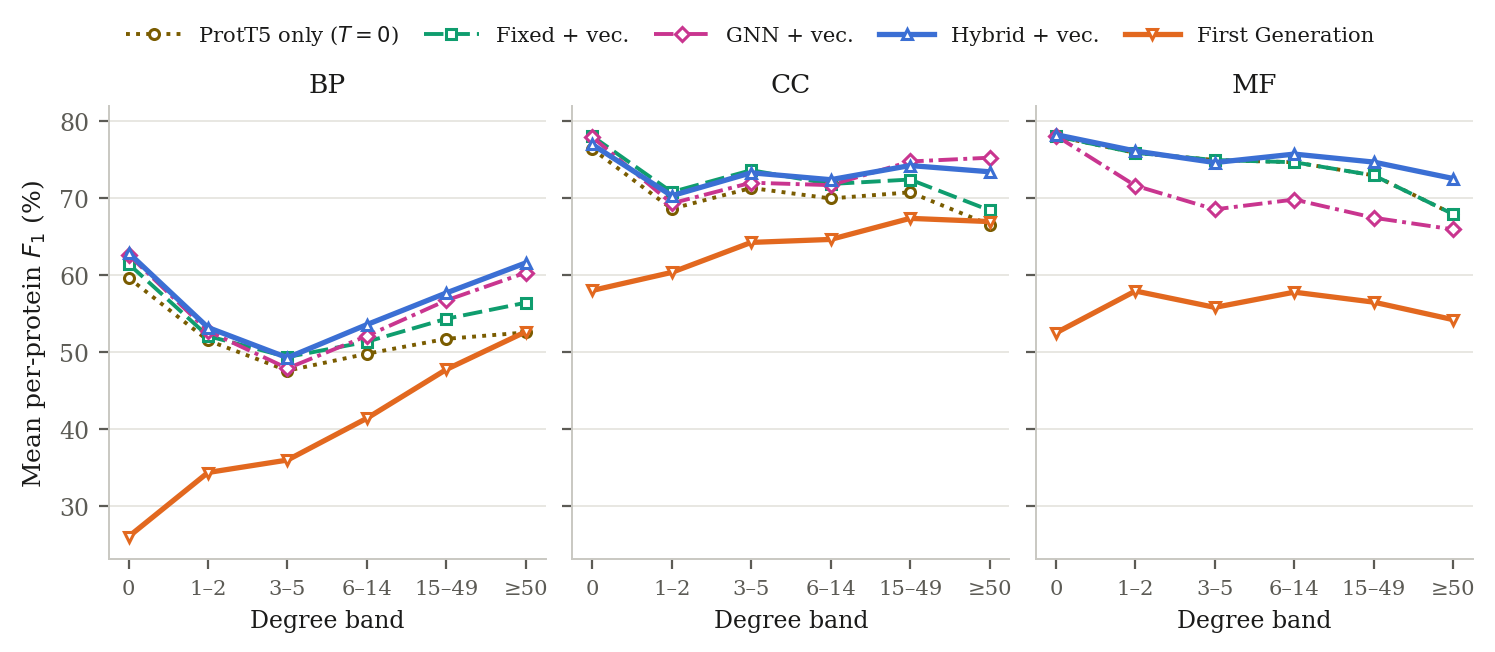
\includegraphics[width=802.5\px,height=350\px]{figures/fig_6_6.png}};
\node[tl] at (88,70) {\fmR\fz{16}{16}\color{inkii}\ls{2}\Ll{5 · Results}};
\node[tl] at (88,131) {\fdA\fz{54}{56.7}\color{ink}\ls{-1}\Ll{The graph helps where there is graph}};
\node<2-4>[tl] at (88,623) {\fmR\fz{15}{19.5}\color{muted}\Ll{Dissertation, Fig. 6.6 · test}};
\node<3-4>[tl] at (1094.7,232) {\fbR\fz{26}{35.1}\color{ink}\Ll{Every ProtT5 route scores worse on\\connected than on isolated proteins}};
\node<3-4>[tl] at (1094.7,318.2) {\fbR\fz{26}{35.1}\color{ink}\Ll{The graph-free control already\\shows it, so the graph does not\\cause it}};
\node<4>[tl] at (1094.7,439.5) {\fbR\fz{26}{35.1}\color{ink}\Ll{The graph's gain grows with degree:\\up to +9.05 BP, +8.71 CC, +4.64 MF\\at degree $\geq$ 50}};
\node[tr] at (1512,876) {\fmR\fz{16}{16}\color{muted}41 / 45};
\end{tikzpicture}
\note{Hubs tend to be multifunctional and harder for a sequence model. In BP the hardest proteins have degree 3 to 5, not zero. 

Degree-zero differences come from rescaling and refitting, so read topological gains from degree one upward.}
\end{frame}

\section{6 · Conclusions}
\begin{frame}[plain]
\begin{tikzpicture}[deck]
\node<1>[box] at (0,0) {\includegraphics[page=3,width=1600\px]{build/layers}};
\node<2>[box] at (0,0) {\includegraphics[page=146,width=1600\px]{build/layers}};
\node<3>[box] at (0,0) {\includegraphics[page=147,width=1600\px]{build/layers}};
\node<4>[box] at (0,0) {\includegraphics[page=148,width=1600\px]{build/layers}};
\node[tl] at (88,70) {\fmR\fz{16}{16}\color{inkii}\ls{2}\Ll{6 · Conclusions}};
\node[tl] at (88,131) {\fdA\fz{54}{56.7}\color{ink}\ls{-1}\Ll{Answers to the research questions}};
\node<2-4>[tc] at (126,232) {\fmM\fz{20}{20}\color{ink}\Lc{RQ1}};
\node<2-4>[tl] at (184,232) {\fbR\fz{20}{26}\color{inkii}\Ll{Which network representation works best?}};
\node<2-4>[tl] at (184,266) {\fbR\fz{27}{35.1}\color{ink}\Ll{The unreduced profile and an MLP; imposed locality hurts}};
\node<2-4>[tc] at (126,321.1) {\fmM\fz{20}{20}\color{ink}\Lc{RQ2}};
\node<2-4>[tl] at (184,321.1) {\fbR\fz{20}{26}\color{inkii}\Ll{How much does propagating ProtT5 over STRING add?}};
\node<2-4>[tl] at (184,355.1) {\fbR\fz{27}{35.1}\color{ink}\Ll{Large gain, mostly from ProtT5; propagation adds +1.87 BP, +2.15 CC, nothing in MF (test)}};
\node<2-4>[tc] at (126,410.2) {\fmM\fz{20}{20}\color{ink}\Lc{RQ3}};
\node<2-4>[tl] at (184,410.2) {\fbR\fz{20}{26}\color{inkii}\Ll{Fixed vs learned aggregation, vector vs image heads}};
\node<2-4>[tl] at (184,444.2) {\fbR\fz{27}{35.1}\color{ink}\Ll{Late 67.06 > Early 65.84 > Fixed 65.12 > GNN 63.32 (validation); vector head throughout}};
\node<3-4>[tc] at (126,499.3) {\fmM\fz{20}{20}\color{ink}\Lc{RQ4}};
\node<3-4>[tl] at (184,499.3) {\fbR\fz{20}{26}\color{inkii}\Ll{Do early and late fusion help?}};
\node<3-4>[tl] at (184,533.3) {\fbR\fz{27}{35.1}\color{ink}\Ll{Both help; late more (+1.26 to +2.18 pp, validation)}};
\node<3-4>[tc] at (126,588.4) {\fmM\fz{20}{20}\color{ink}\Lc{RQ5}};
\node<3-4>[tl] at (184,588.4) {\fbR\fz{20}{26}\color{inkii}\Ll{How deep, and how much retention?}};
\node<3-4>[tl] at (184,622.4) {\fbR\fz{27}{35.1}\color{ink}\Ll{One or two hops, {\fz{30.3}{36.3}$\alpha$} 0.7 to 0.8; MF prefers none}};
\node<4>[tc] at (126,677.5) {\fmM\fz{20}{20}\color{ink}\Lc{RQ6}};
\node<4>[tl] at (184,677.5) {\fbR\fz{20}{26}\color{inkii}\Ll{How does it compare with the literature?}};
\node<4>[tl] at (184,711.5) {\fbR\fz{27}{35.1}\color{ink}\Ll{Best in every column but one; +9.77 / +8.67 / +4.93 pp wF\textsubscript{max} (test)}};
\node<4>[tc] at (126,766.6) {\fmM\fz{20}{20}\color{ink}\Lc{RQ7}};
\node<4>[tl] at (184,766.6) {\fbR\fz{20}{26}\color{inkii}\Ll{Does it work on one global, aggregated network?}};
\node<4>[tl] at (184,800.6) {\fbR\fz{27}{35.1}\color{ink}\Ll{Works on one global aggregated network; partitioned graphs not tested}};
\node[tr] at (1512,876) {\fmR\fz{16}{16}\color{muted}42 / 45};
\end{tikzpicture}
\note{Use the conclusions chapter wording if asked for detail. 

RQ7 is applicability, not superiority over partitioned graphs.}
\end{frame}

\begin{frame}[plain]
\begin{tikzpicture}[deck]
\node<1>[box] at (0,0) {\includegraphics[page=3,width=1600\px]{build/layers}};
\node<2>[box] at (0,0) {\includegraphics[page=149,width=1600\px]{build/layers}};
\node<3>[box] at (0,0) {\includegraphics[page=150,width=1600\px]{build/layers}};
\node<4>[box] at (0,0) {\includegraphics[page=151,width=1600\px]{build/layers}};
\node[tl] at (88,70) {\fmR\fz{16}{16}\color{inkii}\ls{2}\Ll{6 · Conclusions}};
\node[tl] at (88,131) {\fdA\fz{54}{56.7}\color{ink}\ls{-1}\Ll{Limitations}};
\node<2-4>[tl] at (124,236) {\fbR\fz{30}{40.5}\color{ink}\Ll{Single seed; the 0.5 pp floor is a reading convention, not a confidence interval}};
\node<2-4>[tl] at (124,298.5) {\fbR\fz{30}{40.5}\color{ink}\Ll{Random protein-level split: transductive interpolation, possible homology leakage}};
\node<3-4>[tl] at (124,361) {\fbR\fz{30}{40.5}\color{ink}\Ll{STRING scores may encode annotation knowledge (circularity)}};
\node<4>[tl] at (124,423.5) {\fbR\fz{30}{40.5}\color{ink}\Ll{Fixed vs learned is not a single-factor ablation ({\fz{33.7}{40.4}$\alpha^{T}$} scaling, normalization)}};
\node<4>[tl] at (124,486) {\fbR\fz{30}{40.5}\color{ink}\Ll{Baselines adapted to one aggregated network and a reduced label space}};
\node[tr] at (1512,876) {\fmR\fz{16}{16}\color{muted}43 / 45};
\end{tikzpicture}
\note{State these before the committee does. 

Each one is documented in the dissertation with its consequence.}
\end{frame}

\begin{frame}[plain]
\begin{tikzpicture}[deck]
\node<1>[box] at (0,0) {\includegraphics[page=3,width=1600\px]{build/layers}};
\node<2>[box] at (0,0) {\includegraphics[page=152,width=1600\px]{build/layers}};
\node<3>[box] at (0,0) {\includegraphics[page=153,width=1600\px]{build/layers}};
\node[tl] at (88,70) {\fmR\fz{16}{16}\color{inkii}\ls{2}\Ll{6 · Conclusions}};
\node[tl] at (88,131) {\fdA\fz{54}{56.7}\color{ink}\ls{-1}\Ll{Next steps}};
\node<2-3>[tl] at (115,337) {\fbR\fz{27}{35.1}\color{ink}\Ll{Separate the graph by organism,\\or one model per organism}};
\node<2-3>[tl] at (599,337) {\fbR\fz{27}{35.1}\color{ink}\Ll{Keep STRING evidence channels\\apart (typed or parallel edges)}};
\node<2-3>[tl] at (1083,337) {\fbR\fz{27}{35.1}\color{ink}\Ll{Heterogeneous graphs (proteins,\\terms, evidence); compare with\\ProtHGT}};
\node<3>[tl] at (357,604.3) {\fbR\fz{27}{35.1}\color{ink}\Ll{Sampled aggregation\\(GraphSAGE) for a cheaper\\learned route}};
\node<3>[tl] at (841,604.3) {\fbR\fz{27}{35.1}\color{ink}\Ll{Richer node features: structure,\\domains, expression; most\\promising for MF}};
\node[tr] at (1512,876) {\fmR\fz{16}{16}\color{muted}44 / 45};
\end{tikzpicture}
\note{The two most immediate are taxonomic scope and evidence channels. 

MF is where the network contributed least, so new node features matter most there.}
\end{frame}

\begin{frame}[plain]
\begin{tikzpicture}[deck]
\node[box] at (0,0) {\includegraphics[page=154,width=1600\px]{build/layers}};
\node[tl] at (88,367) {\fdB\fz{104}{98.8}\color{ink}\ls{-2.5}\Ll{Thank you}};
\node[tl] at (124,412.8) {\fbR\fz{30}{40.5}\color{ink}\Ll{NEXUS-GO: fixed propagation of ProtT5 over STRING, fused with a GCN, best in every\\ontology at a fraction of the cost}};
\node[tl] at (124,515.8) {\fbR\fz{30}{40.5}\color{ink}\Ll{Code: {\fmR\fz{25.8}{31}{}github.com/ymauhn/nexus-go}}};
\node[tl] at (124,578.3) {\fbR\fz{30}{40.5}\color{ink}\Ll{Publications: VISAPP 2026; extended version accepted in CCIS (expected December 2026)}};
\node[tl] at (124,640.8) {\fbR\fz{30}{40.5}\color{ink}\Ll{Funding: CAPES, BTG Pactual · Computing resources: IC/Unicamp}};
\node[tl] at (88,829) {\fdA\fz{40}{40}\color{ink}\Ll{Questions}};
\end{tikzpicture}
\note{Thank the committee, the advisors and the funders. 

Open for questions.}
\end{frame}

\section{Backup}
\begin{frame}[plain]
\begin{tikzpicture}[deck]
\node[box] at (0,0) {\includegraphics[page=155,width=1600\px]{build/layers}};
\node[tl] at (88,70) {\fmR\fz{16}{16}\color{inkii}\ls{2}\Ll{Backup}};
\node[tl] at (88,131) {\fdA\fz{54}{56.7}\color{ink}\ls{-1}\Ll{Hyperparameters}};
\node[tl] at (100,230) {\fbB\fz{20}{24}\color{inkii}\Ll{Setting}};
\node[tl] at (320.5,230) {\fbB\fz{20}{24}\color{inkii}\Ll{Value}};
\node[tl] at (499,230) {\fbB\fz{20}{24}\color{inkii}\Ll{Scope}};
\node[tl] at (100,264) {\fbR\fz{18}{21.6}\color{ink}\Ll{Optimizer}};
\node[tl] at (320.5,264) {\fbR\fz{18}{21.6}\color{ink}\Ll{Adam}};
\node[tl] at (499,264) {\fbR\fz{18}{21.6}\color{ink}\Ll{all families}};
\node[tl] at (100,299) {\fbR\fz{18}{21.6}\color{ink}\Ll{Learning rate}};
\node[tl] at (320.5,299) {\fbR\fz{18}{21.6}\color{ink}\Ll{1 × 10\textsuperscript{-4}}};
\node[tl] at (499,299) {\fbR\fz{18}{21.6}\color{ink}\Ll{all families}};
\node[tl] at (100,334) {\fbR\fz{18}{21.6}\color{ink}\Ll{Weight decay}};
\node[tl] at (320.5,334) {\fbR\fz{18}{21.6}\color{ink}\Ll{none}};
\node[tl] at (499,334) {\fbR\fz{18}{21.6}\color{ink}\Ll{all families}};
\node[tl] at (100,369) {\fbR\fz{18}{21.6}\color{ink}\Ll{Learning-rate schedule}};
\node[tl] at (320.5,369) {\fbR\fz{18}{21.6}\color{ink}\Ll{none}};
\node[tl] at (499,369) {\fbR\fz{18}{21.6}\color{ink}\Ll{all families}};
\node[tl] at (100,404) {\fbR\fz{18}{21.6}\color{ink}\Ll{Batch size}};
\node[tl] at (320.5,404) {\fbR\fz{18}{21.6}\color{ink}\Ll{256}};
\node[tl] at (499,404) {\fbR\fz{18}{21.6}\color{ink}\Ll{all families}};
\node[tl] at (100,439) {\fbR\fz{18}{21.6}\color{ink}\Ll{Maximum epochs}};
\node[tl] at (320.5,439) {\fbR\fz{18}{21.6}\color{ink}\Ll{250}};
\node[tl] at (499,439) {\fbR\fz{18}{21.6}\color{ink}\Ll{all families}};
\node[tl] at (100,474) {\fbR\fz{18}{21.6}\color{ink}\Ll{Early-stopping patience}};
\node[tl] at (320.5,474) {\fbR\fz{18}{21.6}\color{ink}\Ll{20 epochs}};
\node[tl] at (499,474) {\fbR\fz{18}{21.6}\color{ink}\Ll{all families}};
\node[tl] at (100,509) {\fbR\fz{18}{21.6}\color{ink}\Ll{Monitored quantity}};
\node[tl] at (320.5,509) {\fbR\fz{18}{21.6}\color{ink}\Ll{validation loss}};
\node[tl] at (499,509) {\fbR\fz{18}{21.6}\color{ink}\Ll{all families}};
\node[tl] at (100,544) {\fbR\fz{18}{21.6}\color{ink}\Ll{Minimum improvement}};
\node[tl] at (320.5,544) {\fbR\fz{18}{21.6}\color{ink}\Ll{0}};
\node[tl] at (499,544) {\fbR\fz{18}{21.6}\color{ink}\Ll{all families}};
\node[tl] at (100,579) {\fbR\fz{18}{21.6}\color{ink}\Ll{Objective}};
\node[tl] at (320.5,579) {\fbR\fz{18}{21.6}\color{ink}\Ll{Eq. 5.20}};
\node[tl] at (499,579) {\fbR\fz{18}{21.6}\color{ink}\Ll{all families}};
\node[tl] at (100,614) {\fbR\fz{18}{21.6}\color{ink}\Ll{Class weighting}};
\node[tl] at (320.5,614) {\fbR\fz{18}{21.6}\color{ink}\Ll{information content}};
\node[tl] at (499,614) {\fbR\fz{18}{21.6}\color{ink}\Ll{all families}};
\node[tl] at (100,649) {\fbR\fz{18}{21.6}\color{ink}\Ll{Dropout, prediction head}};
\node[tl] at (320.5,649) {\fbR\fz{18}{21.6}\color{ink}\Ll{0.4}};
\node[tl] at (499,649) {\fbR\fz{18}{21.6}\color{ink}\Ll{all families}};
\node[tl] at (88,686) {\fmR\fz{15}{19.5}\color{muted}\Ll{Dissertation, Table A.2}};
\node[tl] at (828,230) {\fbB\fz{20}{24}\color{inkii}\Ll{Setting}};
\node[tl] at (1072.2,230) {\fbB\fz{20}{24}\color{inkii}\Ll{Value}};
\node[tl] at (1359,230) {\fbB\fz{20}{24}\color{inkii}\Ll{Scope}};
\node[tl] at (828,264) {\fbR\fz{18}{24}\color{ink}\Ll{Dropout, between\\convolutions}};
\node[tl] at (1072.2,264) {\fbR\fz{18}{21.6}\color{ink}\Ll{0.3}};
\node[tl] at (1359,264) {\fbR\fz{18}{24}\color{ink}\Ll{graph\\convolutions}};
\node[tl] at (828,323) {\fbR\fz{18}{21.6}\color{ink}\Ll{Hidden widths, head}};
\node[tl] at (1072.2,323) {\fbR\fz{18}{21.6}\color{ink}\Ll{[1024, 512]}};
\node[tl] at (1359,323) {\fbR\fz{18}{21.6}\color{ink}\Ll{all families}};
\node[tl] at (828,358) {\fbR\fz{18}{21.6}\color{ink}\Ll{Convolution hidden width}};
\node[tl] at (1072.2,358) {\fbR\fz{18}{21.6}\color{ink}\Ll{1024}};
\node[tl] at (1359,358) {\fbR\fz{18}{24}\color{ink}\Ll{graph\\convolutions}};
\node[tl] at (828,417) {\fbR\fz{18}{21.6}\color{ink}\Ll{Convolution layers}};
\node[tl] at (1072.2,417) {\fbR\fz{18}{21.6}\color{ink}\Ll{2}};
\node[tl] at (1359,417) {\fbR\fz{18}{24}\color{ink}\Ll{graph\\convolutions}};
\node[tl] at (828,476) {\fbR\fz{18}{21.6}\color{ink}\Ll{Attention heads}};
\node[tl] at (1072.2,476) {\fbR\fz{18}{21.6}\color{ink}\Ll{4 (hidden), 1 (output)}};
\node[tl] at (1359,476) {\fbR\fz{18}{21.6}\color{ink}\Ll{graph attention}};
\node[tl] at (828,511) {\fbR\fz{18}{21.6}\color{ink}\Ll{Random seed}};
\node[tl] at (1072.2,511) {\fbR\fz{18}{21.6}\color{ink}\Ll{1337}};
\node[tl] at (1359,511) {\fbR\fz{18}{21.6}\color{ink}\Ll{all families}};
\node[tl] at (828,546) {\fbR\fz{18}{21.6}\color{ink}\Ll{Data-loading workers}};
\node[tl] at (1072.2,546) {\fbR\fz{18}{21.6}\color{ink}\Ll{4}};
\node[tl] at (1359,546) {\fbR\fz{18}{21.6}\color{ink}\Ll{all families}};
\node[tl] at (828,581) {\fbR\fz{18}{21.6}\color{ink}\Ll{Configured edge threshold}};
\node[tl] at (1072.2,581) {\fbR\fz{18}{24}\color{ink}\Ll{0.10 (inert; source-data floor =\\0.400)}};
\node[tl] at (1359,581) {\fbR\fz{18}{21.6}\color{ink}\Ll{all families}};
\node[tl] at (828,640) {\fbR\fz{18}{21.6}\color{ink}\Ll{Propagation steps T}};
\node[tl] at (1072.2,640) {\fbR\fz{18}{21.6}\color{ink}\Ll{varies}};
\node[tl] at (1359,640) {\fbR\fz{18}{21.6}\color{ink}\Ll{fixed propagation}};
\node[tl] at (828,676) {\fbR\fz{18}{21.6}\color{ink}\Ll{Mixing coefficient $\alpha$}};
\node[tl] at (1072.2,675) {\fbR\fz{18}{21.6}\color{ink}\Ll{varies}};
\node[tl] at (1359,675) {\fbR\fz{18}{21.6}\color{ink}\Ll{fixed propagation}};
\node[tl] at (828,711) {\fbR\fz{18}{21.6}\color{ink}\Ll{Deduplication rule}};
\node[tl] at (1072.2,711) {\fbR\fz{18}{21.6}\color{ink}\Ll{varies}};
\node[tl] at (1359,711) {\fbR\fz{18}{21.6}\color{ink}\Ll{all families}};
\node[tl] at (816,748) {\fmR\fz{15}{19.5}\color{muted}\Ll{Dissertation, Table A.2}};
\node[tr] at (1512,876) {\fmR\fz{16}{16}\color{muted}B1};
\end{tikzpicture}
\note{Optimization settings of the final second-generation campaign (Table A.2). Values marked varies are part of the search space.}
\end{frame}

\begin{frame}[plain]
\begin{tikzpicture}[deck]
\node[box] at (0,0) {\includegraphics[page=156,width=1600\px]{build/layers}};
\node[tl] at (88,70) {\fmR\fz{16}{16}\color{inkii}\ls{2}\Ll{Backup}};
\node[tl] at (88,131) {\fdA\fz{54}{56.7}\color{ink}\ls{-1}\Ll{Late fusion: grid and selected coefficients}};
\node[tl] at (100,230) {\fbB\fz{20}{24}\color{inkii}\Ll{Rule}};
\node[tl] at (381.2,230) {\fbB\fz{20}{24}\color{inkii}\Ll{Grid}};
\node[tl] at (826.4,230) {\fbB\fz{20}{24}\color{inkii}\Ll{Config.}};
\node[tl] at (100,264) {\fbR\fz{18}{21.6}\color{ink}\Ll{Linear combination}};
\node[tl] at (381.2,265) {\fbR\fz{18}{21.6}\color{ink}\Ll{$\gamma$ from 0.00 to 1.00 in steps of 0.05}};
\node[tl] at (826.4,264) {\fbR\fz{18}{21.6}\color{ink}\Ll{21}};
\node[tl] at (100,300) {\fbR\fz{18}{24}\color{ink}\Ll{Pointwise maximum and\\minimum}};
\node[tl] at (381.2,300) {\fbR\fz{18}{21.6}\color{ink}\Ll{no parameter}};
\node[tl] at (826.4,300) {\fbR\fz{18}{21.6}\color{ink}\Ll{2}};
\node[tl] at (100,359) {\fbR\fz{18}{21.6}\color{ink}\Ll{Term-specific weighting}};
\node[tl] at (381.2,360) {\fbR\fz{18}{21.6}\color{ink}\Ll{IC\textsubscript{thr} $\in$ \{0.4, 1.1, 2.1, 3.4\} and $\kappa$\textsubscript{IC} $\in$ \{1, 2, 5\}}};
\node[tl] at (826.4,359) {\fbR\fz{18}{21.6}\color{ink}\Ll{12}};
\node[tl] at (100,395) {\fbR\fz{18}{21.6}\color{ink}\Ll{Protein-specific weighting}};
\node[tl] at (381.2,396) {\fbR\fz{18}{24}\color{ink}\Ll{d\textsubscript{thr} $\in$ \{1, 3, 5, 14, 28\} and $\kappa$\textsubscript{deg} $\in$ \{0.25, 0.50, 0.75,\\1.00\}}};
\node[tl] at (826.4,395) {\fbR\fz{18}{21.6}\color{ink}\Ll{20}};
\node[tl] at (100,455) {\fbR\fz{18}{21.6}\color{ink}\Ll{Combined weighting}};
\node[tl] at (381.2,456) {\fbR\fz{18}{21.6}\color{ink}\Ll{$\lambda$ from 0.0 to 1.0 in steps of 0.1}};
\node[tl] at (826.4,455) {\fbR\fz{18}{21.6}\color{ink}\Ll{11}};
\node[tl] at (100,491) {\fbR\fz{18}{21.6}\color{ink}\Ll{Stacking}};
\node[tl] at (381.2,491) {\fbR\fz{18}{21.6}\color{ink}\Ll{five meta-classifiers, no coefficient swept}};
\node[tl] at (826.4,491) {\fbR\fz{18}{21.6}\color{ink}\Ll{5}};
\node[tl] at (100,526) {\fbR\fz{18}{21.6}\color{ink}\Ll{Total}};
\node[tl] at (826.4,526) {\fbR\fz{18}{21.6}\color{ink}\Ll{71}};
\node[tl] at (88,563) {\fmR\fz{15}{19.5}\color{muted}\Ll{Dissertation, Table A.3}};
\node[tl] at (949.3,230) {\fbB\fz{20}{24}\color{inkii}\Ll{Rule}};
\node[tr] at (1281.6,230) {\fbB\fz{20}{24}\color{inkii}\Lr{Coefficient}};
\node[tr] at (1348.8,230) {\fbB\fz{20}{24}\color{inkii}\Lr{BP}};
\node[tr] at (1416,230) {\fbB\fz{20}{24}\color{inkii}\Lr{CC}};
\node[tr] at (1483.2,230) {\fbB\fz{20}{24}\color{inkii}\Lr{MF}};
\node[tl] at (949.3,264) {\fbR\fz{18}{21.6}\color{ink}\Ll{Linear combination}};
\node[tr] at (1281.6,264.5) {\fmR\fz{18}{21.6}\color{ink}\Lr{$\gamma$}};
\node[tr] at (1348.8,264.5) {\fmR\fz{18}{21.6}\color{ink}\Lr{0.50}};
\node[tr] at (1416,264.5) {\fmR\fz{18}{21.6}\color{ink}\Lr{0.55}};
\node[tr] at (1483.2,264.5) {\fmR\fz{18}{21.6}\color{ink}\Lr{0.55}};
\node[tl] at (949.3,299) {\fbR\fz{18}{21.6}\color{ink}\Ll{Term-specific weighting}};
\node[tr] at (1281.6,299.5) {\fmR\fz{18}{21.6}\color{ink}\Lr{IC\textsubscript{thr}}};
\node[tr] at (1348.8,299.5) {\fmR\fz{18}{21.6}\color{ink}\Lr{1.1}};
\node[tr] at (1416,299.5) {\fmR\fz{18}{21.6}\color{ink}\Lr{0.4}};
\node[tr] at (1483.2,299.5) {\fmR\fz{18}{21.6}\color{ink}\Lr{0.4}};
\node[tr] at (1281.6,334) {\fmR\fz{18}{21.6}\color{ink}\Lr{$\kappa$\textsubscript{IC}}};
\node[tr] at (1348.8,334) {\fmR\fz{18}{21.6}\color{ink}\Lr{1.0}};
\node[tr] at (1416,334) {\fmR\fz{18}{21.6}\color{ink}\Lr{1.0}};
\node[tr] at (1483.2,334) {\fmR\fz{18}{21.6}\color{ink}\Lr{1.0}};
\node[tl] at (949.3,368) {\fbR\fz{18}{21.6}\color{ink}\Ll{Protein-specific weighting}};
\node[tr] at (1281.6,368.5) {\fmR\fz{18}{21.6}\color{ink}\Lr{d\textsubscript{thr}}};
\node[tr] at (1348.8,368.5) {\fmR\fz{18}{21.6}\color{ink}\Lr{3}};
\node[tr] at (1416,368.5) {\fmR\fz{18}{21.6}\color{ink}\Lr{14}};
\node[tr] at (1483.2,368.5) {\fmR\fz{18}{21.6}\color{ink}\Lr{28}};
\node[tr] at (1281.6,403) {\fmR\fz{18}{21.6}\color{ink}\Lr{$\kappa$\textsubscript{deg}}};
\node[tr] at (1348.8,403) {\fmR\fz{18}{21.6}\color{ink}\Lr{0.25}};
\node[tr] at (1416,403) {\fmR\fz{18}{21.6}\color{ink}\Lr{0.25}};
\node[tr] at (1483.2,403) {\fmR\fz{18}{21.6}\color{ink}\Lr{0.25}};
\node[tl] at (949.3,437) {\fbR\fz{18}{21.6}\color{ink}\Ll{Combined weighting}};
\node[tr] at (1281.6,437.5) {\fmR\fz{18}{21.6}\color{ink}\Lr{$\lambda$}};
\node[tr] at (1348.8,437.5) {\fmR\fz{18}{21.6}\color{ink}\Lr{0.5}};
\node[tr] at (1416,437.5) {\fmR\fz{18}{21.6}\color{ink}\Lr{0.4}};
\node[tr] at (1483.2,437.5) {\fmR\fz{18}{21.6}\color{ink}\Lr{0.9}};
\node[tl] at (937.3,474) {\fmR\fz{15}{19.5}\color{muted}\Ll{Dissertation, Table A.4}};
\node[tr] at (1512,876) {\fmR\fz{16}{16}\color{muted}B2};
\end{tikzpicture}
\note{71 configurations per ontology, chosen on validation. Both conditional rules converged on the flattest sigmoid the grid offers.}
\end{frame}

\begin{frame}[plain]
\begin{tikzpicture}[deck]
\node[box] at (0,0) {\includegraphics[page=157,width=1600\px]{build/layers}};
\node[tl] at (88,70) {\fmR\fz{16}{16}\color{inkii}\ls{2}\Ll{Backup}};
\node[tl] at (88,131) {\fdA\fz{54}{56.7}\color{ink}\ls{-1}\Ll{Early fusion: provenance × source}};
\node[tl] at (100,230) {\fbB\fz{20}{24}\color{inkii}\Ll{Head}};
\node[tr] at (239.5,230) {\fbB\fz{20}{24}\color{inkii}\Lr{Fusion}};
\node[tr] at (371,230) {\fbB\fz{20}{24}\color{inkii}\Lr{Provenance}};
\node[tr] at (459.8,230) {\fbB\fz{20}{24}\color{inkii}\Lr{Source}};
\node[tr] at (537.8,230) {\fbB\fz{20}{24}\color{inkii}\Lr{BP}};
\node[tr] at (615.8,230) {\fbB\fz{20}{24}\color{inkii}\Lr{CC}};
\node[tr] at (693.8,230) {\fbB\fz{20}{24}\color{inkii}\Lr{MF}};
\node[tl] at (100,264) {\fbR\fz{18}{21.6}\color{ink}\Ll{Vector}};
\node[tr] at (239.5,264.5) {\fmR\fz{18}{21.6}\color{ink}\Lr{add}};
\node[tr] at (371,264.5) {\fmR\fz{18}{21.6}\color{ink}\Lr{vector}};
\node[tr] at (459.8,264.5) {\fmR\fz{18}{21.6}\color{ink}\Lr{vector}};
\node[tr] at (537.8,264.5) {\fmR\fz{18}{21.6}\color{ink}\Lr{56.52}};
\node[tr] at (615.8,264.5) {\fmR\fz{18}{21.6}\color{ink}\Lr{66.86}};
\node[tr] at (693.8,264.5) {\fmR\fz{18}{21.6}\color{ink}\Lr{73.81}};
\node[tr] at (239.5,299) {\fmR\fz{18}{21.6}\color{ink}\Lr{add}};
\node[tr] at (371,299) {\fmR\fz{18}{21.6}\color{ink}\Lr{vector}};
\node[tr] at (459.8,299) {\fmR\fz{18}{21.6}\color{ink}\Lr{vision}};
\node[tr] at (537.8,299) {\fmR\fz{18}{21.6}\color{ink}\Lr{55.73}};
\node[tr] at (615.8,299) {\fmR\fz{18}{21.6}\color{ink}\Lr{65.79}};
\node[tr] at (693.8,299) {\fmR\fz{18}{21.6}\color{ink}\Lr{n/a}};
\node[tr] at (239.5,333) {\fmR\fz{18}{21.6}\color{ink}\Lr{add}};
\node[tr] at (371,333) {\fmR\fz{18}{21.6}\color{ink}\Lr{vision}};
\node[tr] at (459.8,333) {\fmR\fz{18}{21.6}\color{ink}\Lr{vector}};
\node[tr] at (537.8,333) {\fmR\fz{18}{21.6}\color{ink}\Lr{53.98}};
\node[tr] at (615.8,333) {\fmR\fz{18}{21.6}\color{ink}\Lr{67.07}};
\node[tr] at (693.8,333) {\fmR\fz{18}{21.6}\color{ink}\Lr{73.42}};
\node[tr] at (239.5,367) {\fmR\fz{18}{21.6}\color{ink}\Lr{add}};
\node[tr] at (371,367) {\fmR\fz{18}{21.6}\color{ink}\Lr{vision}};
\node[tr] at (459.8,367) {\fmR\fz{18}{21.6}\color{ink}\Lr{vision}};
\node[tr] at (537.8,367) {\fmR\fz{18}{21.6}\color{ink}\Lr{52.96}};
\node[tr] at (615.8,367) {\fmR\fz{18}{21.6}\color{ink}\Lr{65.46}};
\node[tr] at (693.8,367) {\fmR\fz{18}{21.6}\color{ink}\Lr{n/a}};
\node[tr] at (239.5,401) {\fmR\fz{18}{21.6}\color{ink}\Lr{concat}};
\node[tr] at (371,401) {\fmR\fz{18}{21.6}\color{ink}\Lr{vector}};
\node[tr] at (459.8,401) {\fmR\fz{18}{21.6}\color{ink}\Lr{vector}};
\node[tr] at (537.8,401) {\fmR\fz{18}{21.6}\color{ink}\Lr{56.05}};
\node[tr] at (615.8,401) {\fmR\fz{18}{21.6}\color{ink}\Lr{67.12}};
\node[tr] at (693.8,401) {\fmR\fz{18}{21.6}\color{ink}\Lr{73.68}};
\node[tr] at (239.5,435) {\fmR\fz{18}{21.6}\color{ink}\Lr{concat}};
\node[tr] at (371,435) {\fmR\fz{18}{21.6}\color{ink}\Lr{vector}};
\node[tr] at (459.8,435) {\fmR\fz{18}{21.6}\color{ink}\Lr{vision}};
\node[tr] at (537.8,435) {\fmR\fz{18}{21.6}\color{ink}\Lr{55.52}};
\node[tr] at (615.8,435) {\fmR\fz{18}{21.6}\color{ink}\Lr{65.27}};
\node[tr] at (693.8,435) {\fmR\fz{18}{21.6}\color{ink}\Lr{n/a}};
\node[tr] at (239.5,469) {\fmR\fz{18}{21.6}\color{ink}\Lr{concat}};
\node[tr] at (371,469) {\fmR\fz{18}{21.6}\color{ink}\Lr{vision}};
\node[tr] at (459.8,469) {\fmR\fz{18}{21.6}\color{ink}\Lr{vector}};
\node[tr] at (537.8,469) {\fmR\fz{18}{21.6}\color{ink}\Lr{55.32}};
\node[tr] at (615.8,469) {\fmR\fz{18}{21.6}\color{ink}\Lr{67.20}};
\node[tr] at (693.8,469) {\fmR\fz{18}{21.6}\color{ink}\Lr{73.78}};
\node[tr] at (239.5,503) {\fmR\fz{18}{21.6}\color{ink}\Lr{concat}};
\node[tr] at (371,503) {\fmR\fz{18}{21.6}\color{ink}\Lr{vision}};
\node[tr] at (459.8,503) {\fmR\fz{18}{21.6}\color{ink}\Lr{vision}};
\node[tr] at (537.8,503) {\fmR\fz{18}{21.6}\color{ink}\Lr{53.23}};
\node[tr] at (615.8,503) {\fmR\fz{18}{21.6}\color{ink}\Lr{65.42}};
\node[tr] at (693.8,503) {\fmR\fz{18}{21.6}\color{ink}\Lr{n/a}};
\node[tl] at (100,537) {\fbR\fz{18}{21.6}\color{ink}\Ll{Vision}};
\node[tr] at (239.5,537.5) {\fmR\fz{18}{21.6}\color{ink}\Lr{add}};
\node[tr] at (371,537.5) {\fmR\fz{18}{21.6}\color{ink}\Lr{vector}};
\node[tr] at (459.8,537.5) {\fmR\fz{18}{21.6}\color{ink}\Lr{vector}};
\node[tr] at (537.8,537.5) {\fmR\fz{18}{21.6}\color{ink}\Lr{52.36}};
\node[tr] at (615.8,537.5) {\fmR\fz{18}{21.6}\color{ink}\Lr{64.77}};
\node[tr] at (693.8,537.5) {\fmR\fz{18}{21.6}\color{ink}\Lr{69.52}};
\node[tr] at (239.5,572) {\fmR\fz{18}{21.6}\color{ink}\Lr{add}};
\node[tr] at (371,572) {\fmR\fz{18}{21.6}\color{ink}\Lr{vector}};
\node[tr] at (459.8,572) {\fmR\fz{18}{21.6}\color{ink}\Lr{vision}};
\node[tr] at (537.8,572) {\fmR\fz{18}{21.6}\color{ink}\Lr{53.17}};
\node[tr] at (615.8,572) {\fmR\fz{18}{21.6}\color{ink}\Lr{64.71}};
\node[tr] at (693.8,572) {\fmR\fz{18}{21.6}\color{ink}\Lr{n/a}};
\node[tr] at (239.5,606) {\fmR\fz{18}{21.6}\color{ink}\Lr{add}};
\node[tr] at (371,606) {\fmR\fz{18}{21.6}\color{ink}\Lr{vision}};
\node[tr] at (459.8,606) {\fmR\fz{18}{21.6}\color{ink}\Lr{vector}};
\node[tr] at (537.8,606) {\fmR\fz{18}{21.6}\color{ink}\Lr{49.72}};
\node[tr] at (615.8,606) {\fmR\fz{18}{21.6}\color{ink}\Lr{62.66}};
\node[tr] at (693.8,606) {\fmR\fz{18}{21.6}\color{ink}\Lr{67.66}};
\node[tr] at (239.5,640) {\fmR\fz{18}{21.6}\color{ink}\Lr{add}};
\node[tr] at (371,640) {\fmR\fz{18}{21.6}\color{ink}\Lr{vision}};
\node[tr] at (459.8,640) {\fmR\fz{18}{21.6}\color{ink}\Lr{vision}};
\node[tr] at (537.8,640) {\fmR\fz{18}{21.6}\color{ink}\Lr{50.21}};
\node[tr] at (615.8,640) {\fmR\fz{18}{21.6}\color{ink}\Lr{62.64}};
\node[tr] at (693.8,640) {\fmR\fz{18}{21.6}\color{ink}\Lr{n/a}};
\node[tl] at (88,676) {\fmR\fz{15}{19.5}\color{muted}\Ll{Dissertation, Table 6.13}};
\node[tr] at (1512,876) {\fmR\fz{16}{16}\color{muted}B3};
\end{tikzpicture}
\note{Provenance is the head with which the consumed GNN embedding was trained; source is the head whose depth and retention were used for the fixed branch. Validation set.}
\end{frame}

\begin{frame}[plain]
\begin{tikzpicture}[deck]
\node[box] at (0,0) {\includegraphics[page=158,width=1600\px]{build/layers}};
\node[tl] at (88,70) {\fmR\fz{16}{16}\color{inkii}\ls{2}\Ll{Backup}};
\node[tl] at (88,131) {\fdA\fz{54}{56.7}\color{ink}\ls{-1}\Ll{Isolated vs connected proteins}};
\node[tl] at (100,230) {\fbB\fz{20}{24}\color{inkii}\Ll{Route}};
\node[tr] at (601.1,230) {\fbB\fz{20}{24}\color{inkii}\Lr{BP}};
\node[tr] at (845.9,230) {\fbB\fz{20}{24}\color{inkii}\Lr{CC}};
\node[tr] at (1090.7,230) {\fbB\fz{20}{24}\color{inkii}\Lr{MF}};
\node[tr] at (434.3,265) {\fbB\fz{20}{24}\color{inkii}\Lr{Isol.}};
\node[tr] at (512.3,265) {\fbB\fz{20}{24}\color{inkii}\Lr{Conn.}};
\node[tr] at (601.1,265) {\fbB\fz{20}{24}\color{inkii}\Lr{$\Delta$}};
\node[tr] at (679.1,265) {\fbB\fz{20}{24}\color{inkii}\Lr{Isol.}};
\node[tr] at (757.1,265) {\fbB\fz{20}{24}\color{inkii}\Lr{Conn.}};
\node[tr] at (845.9,265) {\fbB\fz{20}{24}\color{inkii}\Lr{$\Delta$}};
\node[tr] at (923.9,265) {\fbB\fz{20}{24}\color{inkii}\Lr{Isol.}};
\node[tr] at (1001.9,265) {\fbB\fz{20}{24}\color{inkii}\Lr{Conn.}};
\node[tr] at (1090.7,265) {\fbB\fz{20}{24}\color{inkii}\Lr{$\Delta$}};
\node[tl] at (100,299) {\fbR\fz{18}{21.6}\color{ink}\Ll{ProtT5 only (T=0)}};
\node[tr] at (434.3,299.5) {\fmR\fz{18}{21.6}\color{ink}\Lr{59.89}};
\node[tr] at (512.3,299.5) {\fmR\fz{18}{21.6}\color{ink}\Lr{50.23}};
\node[tr] at (601.1,299.5) {\fmR\fz{18}{21.6}\color{ink}\Lr{−9.66}};
\node[tr] at (679.1,299.5) {\fmR\fz{18}{21.6}\color{ink}\Lr{69.30}};
\node[tr] at (757.1,299.5) {\fmR\fz{18}{21.6}\color{ink}\Lr{62.38}};
\node[tr] at (845.9,299.5) {\fmR\fz{18}{21.6}\color{ink}\Lr{−6.92}};
\node[tr] at (923.9,299.5) {\fmR\fz{18}{21.6}\color{ink}\Lr{75.68}};
\node[tr] at (1001.9,299.5) {\fmR\fz{18}{21.6}\color{ink}\Lr{71.23}};
\node[tr] at (1090.7,299.5) {\fmR\fz{18}{21.6}\color{ink}\Lr{−4.45}};
\node[tl] at (100,334) {\fbR\fz{18}{21.6}\color{ink}\Ll{Fixed propagation + vector head}};
\node[tr] at (434.3,334.5) {\fmR\fz{18}{21.6}\color{ink}\Lr{61.30}};
\node[tr] at (512.3,334.5) {\fmR\fz{18}{21.6}\color{ink}\Lr{52.39}};
\node[tr] at (601.1,334.5) {\fmR\fz{18}{21.6}\color{ink}\Lr{−8.91}};
\node[tr] at (679.1,334.5) {\fmR\fz{18}{21.6}\color{ink}\Lr{71.12}};
\node[tr] at (757.1,334.5) {\fmR\fz{18}{21.6}\color{ink}\Lr{64.77}};
\node[tr] at (845.9,334.5) {\fmR\fz{18}{21.6}\color{ink}\Lr{−6.35}};
\node[tr] at (923.9,334.5) {\fmR\fz{18}{21.6}\color{ink}\Lr{75.68}};
\node[tr] at (1001.9,334.5) {\fmR\fz{18}{21.6}\color{ink}\Lr{71.23}};
\node[tr] at (1090.7,334.5) {\fmR\fz{18}{21.6}\color{ink}\Lr{−4.45}};
\node[tl] at (100,369) {\fbR\fz{18}{21.6}\color{ink}\Ll{End-to-end GNN + vector head}};
\node[tr] at (434.3,369.5) {\fmR\fz{18}{21.6}\color{ink}\Lr{62.26}};
\node[tr] at (512.3,369.5) {\fmR\fz{18}{21.6}\color{ink}\Lr{53.97}};
\node[tr] at (601.1,369.5) {\fmR\fz{18}{21.6}\color{ink}\Lr{−8.29}};
\node[tr] at (679.1,369.5) {\fmR\fz{18}{21.6}\color{ink}\Lr{70.44}};
\node[tr] at (757.1,369.5) {\fmR\fz{18}{21.6}\color{ink}\Lr{64.76}};
\node[tr] at (845.9,369.5) {\fmR\fz{18}{21.6}\color{ink}\Lr{−5.68}};
\node[tr] at (923.9,369.5) {\fmR\fz{18}{21.6}\color{ink}\Lr{74.99}};
\node[tr] at (1001.9,369.5) {\fmR\fz{18}{21.6}\color{ink}\Lr{64.30}};
\node[tr] at (1090.7,369.5) {\fmR\fz{18}{21.6}\color{ink}\Lr{−10.69}};
\node[tl] at (100,404) {\fbR\fz{18}{21.6}\color{ink}\Ll{Early fusion + vector head}};
\node[tr] at (434.3,404.5) {\fmR\fz{18}{21.6}\color{ink}\Lr{62.46}};
\node[tr] at (512.3,404.5) {\fmR\fz{18}{21.6}\color{ink}\Lr{54.58}};
\node[tr] at (601.1,404.5) {\fmR\fz{18}{21.6}\color{ink}\Lr{−7.88}};
\node[tr] at (679.1,404.5) {\fmR\fz{18}{21.6}\color{ink}\Lr{69.41}};
\node[tr] at (757.1,404.5) {\fmR\fz{18}{21.6}\color{ink}\Lr{66.08}};
\node[tr] at (845.9,404.5) {\fmR\fz{18}{21.6}\color{ink}\Lr{−3.33}};
\node[tr] at (923.9,404.5) {\fmR\fz{18}{21.6}\color{ink}\Lr{74.85}};
\node[tr] at (1001.9,404.5) {\fmR\fz{18}{21.6}\color{ink}\Lr{72.05}};
\node[tr] at (1090.7,404.5) {\fmR\fz{18}{21.6}\color{ink}\Lr{−2.80}};
\node[tl] at (100,439) {\fbR\fz{18}{21.6}\color{ink}\Ll{First Generation}};
\node[tr] at (434.3,439.5) {\fmR\fz{18}{21.6}\color{ink}\Lr{24.86}};
\node[tr] at (512.3,439.5) {\fmR\fz{18}{21.6}\color{ink}\Lr{43.88}};
\node[tr] at (601.1,439.5) {\fmR\fz{18}{21.6}\color{ink}\Lr{+19.02}};
\node[tr] at (679.1,439.5) {\fmR\fz{18}{21.6}\color{ink}\Lr{33.97}};
\node[tr] at (757.1,439.5) {\fmR\fz{18}{21.6}\color{ink}\Lr{53.74}};
\node[tr] at (845.9,439.5) {\fmR\fz{18}{21.6}\color{ink}\Lr{+19.77}};
\node[tr] at (923.9,439.5) {\fmR\fz{18}{21.6}\color{ink}\Lr{35.68}};
\node[tr] at (1001.9,439.5) {\fmR\fz{18}{21.6}\color{ink}\Lr{51.95}};
\node[tr] at (1090.7,439.5) {\fmR\fz{18}{21.6}\color{ink}\Lr{+16.27}};
\node[tl] at (88,476) {\fmR\fz{15}{19.5}\color{muted}\Ll{Dissertation, Table 6.22}};
\node[tr] at (1512,876) {\fmR\fz{16}{16}\color{muted}B4};
\end{tikzpicture}
\note{wF\textsubscript{max} on the test set. Every ProtT5 route scores worse on connected proteins; the First Generation is the only route that improves with connectivity.}
\end{frame}

\begin{frame}[plain]
\begin{tikzpicture}[deck]
\node[box] at (0,0) {\includegraphics[page=159,width=1600\px]{build/layers}};
\node[tl] at (88,70) {\fmR\fz{16}{16}\color{inkii}\ls{2}\Ll{Backup}};
\node[tl] at (88,131) {\fdA\fz{54}{56.7}\color{ink}\ls{-1}\Ll{Degree and per-protein F\textsubscript{{\ls{-1.5}{}1}}}};
\node[tl] at (100,230) {\fbB\fz{20}{24}\color{inkii}\Ll{Route}};
\node[tr] at (590.3,230) {\fbB\fz{20}{24}\color{inkii}\Lr{BP}};
\node[tr] at (824.3,230) {\fbB\fz{20}{24}\color{inkii}\Lr{CC}};
\node[tr] at (1058.3,230) {\fbB\fz{20}{24}\color{inkii}\Lr{MF}};
\node[tr] at (423.5,265) {\fbB\fz{20}{24}\color{inkii}\Lr{$\tau$}};
\node[tr] at (512.3,265) {\fbB\fz{20}{24}\color{inkii}\Lr{$\rho$}};
\node[tr] at (590.3,265) {\fbB\fz{20}{24}\color{inkii}\Lr{F\textsubscript{1}}};
\node[tr] at (657.5,265) {\fbB\fz{20}{24}\color{inkii}\Lr{$\tau$}};
\node[tr] at (746.3,265) {\fbB\fz{20}{24}\color{inkii}\Lr{$\rho$}};
\node[tr] at (824.3,265) {\fbB\fz{20}{24}\color{inkii}\Lr{F\textsubscript{1}}};
\node[tr] at (891.5,265) {\fbB\fz{20}{24}\color{inkii}\Lr{$\tau$}};
\node[tr] at (980.3,265) {\fbB\fz{20}{24}\color{inkii}\Lr{$\rho$}};
\node[tr] at (1058.3,265) {\fbB\fz{20}{24}\color{inkii}\Lr{F\textsubscript{1}}};
\node[tl] at (100,299) {\fbR\fz{18}{21.6}\color{ink}\Ll{ProtT5 only (T=0)}};
\node[tr] at (423.5,299.5) {\fmR\fz{18}{21.6}\color{ink}\Lr{0.51}};
\node[tr] at (512.3,299.5) {\fmR\fz{18}{21.6}\color{ink}\Lr{−0.109}};
\node[tr] at (590.3,299.5) {\fmR\fz{18}{21.6}\color{ink}\Lr{53.84}};
\node[tr] at (657.5,299.5) {\fmR\fz{18}{21.6}\color{ink}\Lr{0.58}};
\node[tr] at (746.3,299.5) {\fmR\fz{18}{21.6}\color{ink}\Lr{−0.129}};
\node[tr] at (824.3,299.5) {\fmR\fz{18}{21.6}\color{ink}\Lr{72.29}};
\node[tr] at (891.5,299.5) {\fmR\fz{18}{21.6}\color{ink}\Lr{0.50}};
\node[tr] at (980.3,299.5) {\fmR\fz{18}{21.6}\color{ink}\Lr{−0.128}};
\node[tr] at (1058.3,299.5) {\fmR\fz{18}{21.6}\color{ink}\Lr{75.19}};
\node[tl] at (100,334) {\fbR\fz{18}{21.6}\color{ink}\Ll{Fixed propagation + vector head}};
\node[tr] at (423.5,334.5) {\fmR\fz{18}{21.6}\color{ink}\Lr{0.50}};
\node[tr] at (512.3,334.5) {\fmR\fz{18}{21.6}\color{ink}\Lr{−0.105}};
\node[tr] at (590.3,334.5) {\fmR\fz{18}{21.6}\color{ink}\Lr{55.77}};
\node[tr] at (657.5,334.5) {\fmR\fz{18}{21.6}\color{ink}\Lr{0.63}};
\node[tr] at (746.3,334.5) {\fmR\fz{18}{21.6}\color{ink}\Lr{−0.133}};
\node[tr] at (824.3,334.5) {\fmR\fz{18}{21.6}\color{ink}\Lr{74.07}};
\node[tr] at (891.5,334.5) {\fmR\fz{18}{21.6}\color{ink}\Lr{0.50}};
\node[tr] at (980.3,334.5) {\fmR\fz{18}{21.6}\color{ink}\Lr{−0.128}};
\node[tr] at (1058.3,334.5) {\fmR\fz{18}{21.6}\color{ink}\Lr{75.19}};
\node[tl] at (100,369) {\fbR\fz{18}{21.6}\color{ink}\Ll{End-to-end GNN + vector head}};
\node[tr] at (423.5,369.5) {\fmR\fz{18}{21.6}\color{ink}\Lr{0.39}};
\node[tr] at (512.3,369.5) {\fmR\fz{18}{21.6}\color{ink}\Lr{−0.083}};
\node[tr] at (590.3,369.5) {\fmR\fz{18}{21.6}\color{ink}\Lr{56.96}};
\node[tr] at (657.5,369.5) {\fmR\fz{18}{21.6}\color{ink}\Lr{0.51}};
\node[tr] at (746.3,369.5) {\fmR\fz{18}{21.6}\color{ink}\Lr{−0.087}};
\node[tr] at (824.3,369.5) {\fmR\fz{18}{21.6}\color{ink}\Lr{74.68}};
\node[tr] at (891.5,369.5) {\fmR\fz{18}{21.6}\color{ink}\Lr{0.51}};
\node[tr] at (980.3,369.5) {\fmR\fz{18}{21.6}\color{ink}\Lr{−0.185}};
\node[tr] at (1058.3,369.5) {\fmR\fz{18}{21.6}\color{ink}\Lr{71.79}};
\node[tl] at (100,404) {\fbR\fz{18}{21.6}\color{ink}\Ll{Early fusion + vector head}};
\node[tr] at (423.5,404.5) {\fmR\fz{18}{21.6}\color{ink}\Lr{0.46}};
\node[tr] at (512.3,404.5) {\fmR\fz{18}{21.6}\color{ink}\Lr{−0.077}};
\node[tr] at (590.3,404.5) {\fmR\fz{18}{21.6}\color{ink}\Lr{57.79}};
\node[tr] at (657.5,404.5) {\fmR\fz{18}{21.6}\color{ink}\Lr{0.59}};
\node[tr] at (746.3,404.5) {\fmR\fz{18}{21.6}\color{ink}\Lr{−0.076}};
\node[tr] at (824.3,404.5) {\fmR\fz{18}{21.6}\color{ink}\Lr{74.46}};
\node[tr] at (891.5,404.5) {\fmR\fz{18}{21.6}\color{ink}\Lr{0.42}};
\node[tr] at (980.3,404.5) {\fmR\fz{18}{21.6}\color{ink}\Lr{−0.110}};
\node[tr] at (1058.3,404.5) {\fmR\fz{18}{21.6}\color{ink}\Lr{76.11}};
\node[tl] at (100,439) {\fbR\fz{18}{21.6}\color{ink}\Ll{First Generation}};
\node[tr] at (423.5,439.5) {\fmR\fz{18}{21.6}\color{ink}\Lr{0.41}};
\node[tr] at (512.3,439.5) {\fmR\fz{18}{21.6}\color{ink}\Lr{+0.415}};
\node[tr] at (590.3,439.5) {\fmR\fz{18}{21.6}\color{ink}\Lr{36.62}};
\node[tr] at (657.5,439.5) {\fmR\fz{18}{21.6}\color{ink}\Lr{0.46}};
\node[tr] at (746.3,439.5) {\fmR\fz{18}{21.6}\color{ink}\Lr{+0.161}};
\node[tr] at (824.3,439.5) {\fmR\fz{18}{21.6}\color{ink}\Lr{62.94}};
\node[tr] at (891.5,439.5) {\fmR\fz{18}{21.6}\color{ink}\Lr{0.49}};
\node[tr] at (980.3,439.5) {\fmR\fz{18}{21.6}\color{ink}\Lr{+0.083}};
\node[tr] at (1058.3,439.5) {\fmR\fz{18}{21.6}\color{ink}\Lr{55.44}};
\node[tl] at (88,476) {\fmR\fz{15}{19.5}\color{muted}\Ll{Dissertation, Table 6.27}};
\node[tr] at (1512,876) {\fmR\fz{16}{16}\color{muted}B5};
\end{tikzpicture}
\note{Rank correlation between degree and per-protein F\textsubscript{1}, test set. All sequence-aware routes have small negative correlations; the graph routes make them less negative.}
\end{frame}

\begin{frame}[plain]
\begin{tikzpicture}[deck]
\node[box] at (0,0) {\includegraphics[page=160,width=1600\px]{build/layers}};
\node[tl] at (88,70) {\fmR\fz{16}{16}\color{inkii}\ls{2}\Ll{Backup}};
\node[tl] at (88,131) {\fdA\fz{54}{56.7}\color{ink}\ls{-1}\Ll{Baselines: adaptations, cost and coverage}};
\node[tl] at (100,230) {\fbB\fz{20}{24}\color{inkii}\Ll{Configuration}};
\node[tl] at (425.6,230) {\fbB\fz{20}{24}\color{inkii}\Ll{Principal adaptations}};
\node[tl] at (100,264) {\fbR\fz{18}{24}\color{ink}\Ll{Mashup (embedding + weighted k-\\NN)}};
\node[tl] at (425.6,264) {\fbR\fz{18}{24}\color{ink}\Ll{Embedding of 500 dimensions; classification by weighted k-nearest-neighbor voting (k = 10) instead of the original support vector\\machine}};
\node[tl] at (100,323) {\fbR\fz{18}{24}\color{ink}\Ll{MELISSA (embedding + weighted k-\\NN with Mashup fallback)}};
\node[tl] at (425.6,323) {\fbR\fz{18}{24}\color{ink}\Ll{Randomized embedding mode, which requires a null cannot-link penalty; two clusters; falls back to the Mashup scores when its own\\neighborhood contains no annotated protein}};
\node[tl] at (100,382) {\fbR\fz{18}{24}\color{ink}\Ll{deepNF (single-network autoencoder\\+ MLP)}};
\node[tl] at (425.6,382) {\fbR\fz{18}{24}\color{ink}\Ll{Single autoencoder instead of the multimodal deep autoencoder; multilayer perceptron classification head instead of the original\\support vector machine; binary cross-entropy objective; method-specific edge-weight construction}};
\node[tl] at (100,441) {\fbR\fz{18}{21.6}\color{ink}\Ll{DeepGraphGO (two-model ensemble)}};
\node[tl] at (425.6,441) {\fbR\fz{18}{24}\color{ink}\Ll{Ported from the graph library version targeted by the original release, whose sampling API no longer exists, to the current one;\\homology search rewritten against the current BLAST interface; InterPro features regenerated; ensemble reduced from three models to\\two}};
\node[tl] at (100,524) {\fbR\fz{18}{24}\color{ink}\Ll{SEGT-GO (no SHAP filtering, two-\\model ensemble)}};
\node[tl] at (425.6,524) {\fbR\fz{18}{24}\color{ink}\Ll{Multi-hop feature construction implemented, since the released pipeline does not include it; SHAP feature filter disabled; batch size\\reduced for the available device}};
\node[tl] at (88,585) {\fmR\fz{15}{19.5}\color{muted}\Ll{Dissertation, Table B.1}};
\node[tl] at (100,631.5) {\fbB\fz{20}{24}\color{inkii}\Ll{Configuration}};
\node[tl] at (251.4,631.5) {\fbB\fz{20}{24}\color{inkii}\Ll{Cost}};
\node[tl] at (1288.6,631.5) {\fbB\fz{20}{24}\color{inkii}\Ll{BP}};
\node[tl] at (1367.1,631.5) {\fbB\fz{20}{24}\color{inkii}\Ll{CC}};
\node[tl] at (1445.5,631.5) {\fbB\fz{20}{24}\color{inkii}\Ll{MF}};
\node[tl] at (100,665.5) {\fbR\fz{18}{21.6}\color{ink}\Ll{Mashup}};
\node[tl] at (251.4,665.5) {\fbR\fz{18}{21.6}\color{ink}\Ll{10.0 h for the embedding, computed once and reused by the three ontologies; minutes per ontology thereafter}};
\node[tl] at (1288.6,665.5) {\fbR\fz{18}{21.6}\color{ink}\Ll{63.6\%}};
\node[tl] at (1367.1,665.5) {\fbR\fz{18}{21.6}\color{ink}\Ll{66.6\%}};
\node[tl] at (1445.5,665.5) {\fbR\fz{18}{21.6}\color{ink}\Ll{68.7\%}};
\node[tl] at (100,700.5) {\fbR\fz{18}{21.6}\color{ink}\Ll{MELISSA}};
\node[tl] at (251.4,701.5) {\fbR\fz{18}{21.6}\color{ink}\Ll{$\approx$ 10.1 h per ontology, since the augmented graph depends on the biclustering of that ontology's annotations; $\approx$ 30.3 h in total}};
\node[tl] at (1288.6,700.5) {\fbR\fz{18}{21.6}\color{ink}\Ll{63.6\%}};
\node[tl] at (1367.1,700.5) {\fbR\fz{18}{21.6}\color{ink}\Ll{66.6\%}};
\node[tl] at (1445.5,700.5) {\fbR\fz{18}{21.6}\color{ink}\Ll{68.7\%}};
\node[tl] at (100,736.5) {\fbR\fz{18}{21.6}\color{ink}\Ll{deepNF}};
\node[tl] at (251.4,736.5) {\fbR\fz{18}{21.6}\color{ink}\Ll{not measured}};
\node[tl] at (1288.6,736.5) {\fbR\fz{18}{21.6}\color{ink}\Ll{63.6\%}};
\node[tl] at (1367.1,736.5) {\fbR\fz{18}{21.6}\color{ink}\Ll{66.6\%}};
\node[tl] at (1445.5,736.5) {\fbR\fz{18}{21.6}\color{ink}\Ll{68.7\%}};
\node[tl] at (100,771.5) {\fbR\fz{18}{21.6}\color{ink}\Ll{DeepGraphGO}};
\node[tl] at (251.4,772.5) {\fbR\fz{18}{24}\color{ink}\Ll{$\approx$ 1 h to train the six models and run inference; the homology search dominates, at approximately three hours per ontology and\\partition}};
\node[tl] at (1288.6,771.5) {\fbR\fz{18}{21.6}\color{ink}\Ll{96.3\%}};
\node[tl] at (1367.1,771.5) {\fbR\fz{18}{21.6}\color{ink}\Ll{95.1\%}};
\node[tl] at (1445.5,771.5) {\fbR\fz{18}{21.6}\color{ink}\Ll{95.7\%}};
\node[tl] at (100,831.5) {\fbR\fz{18}{21.6}\color{ink}\Ll{SEGT-GO}};
\node[tl] at (251.4,831.5) {\fbR\fz{18}{21.6}\color{ink}\Ll{34.6 h for the complete pipeline: six models, inference and metrics}};
\node[tl] at (1288.6,831.5) {\fbR\fz{18}{21.6}\color{ink}\Ll{96.3\%}};
\node[tl] at (1367.1,831.5) {\fbR\fz{18}{21.6}\color{ink}\Ll{95.1\%}};
\node[tl] at (1445.5,831.5) {\fbR\fz{18}{21.6}\color{ink}\Ll{95.7\%}};
\node[tl] at (88,868.5) {\fmR\fz{15}{19.5}\color{muted}\Ll{Dissertation, Table B.2}};
\node[tr] at (1512,876) {\fmR\fz{16}{16}\color{muted}B6};
\end{tikzpicture}
\note{Hyperparameters were taken from each method's reference configuration; changes are hardware constraints, not a search. Coverage is the fraction of test proteins that receive a prediction.}
\end{frame}

\begin{frame}[plain]
\begin{tikzpicture}[deck]
\node[box] at (0,0) {\includegraphics[page=161,width=1600\px]{build/layers}};
\node[tl] at (88,70) {\fmR\fz{16}{16}\color{inkii}\ls{2}\Ll{Backup}};
\node[tl] at (88,131) {\fdA\fz{54}{56.7}\color{ink}\ls{-1}\Ll{Hierarchy closure uses {\fmM\fz{46.4}{55.7}\ls{-1.2}{}is\_a} only}};
\node[tl] at (124,236) {\fbR\fz{30}{40.5}\color{ink}\Ll{Ancestors reachable only through {\fmR\fz{25.8}{31}{}part\_of} do not receive their descendants' scores}};
\node[tl] at (124,298.5) {\fbR\fz{30}{40.5}\color{ink}\Ll{Affects 387 of 3,507 ancestor-descendant pairs in BP (11.0\%), 2,056 of 4,405 in CC (46.7\%), a single\\pair in MF}};
\node[tl] at (124,401.5) {\fbR\fz{30}{40.5}\color{ink}\Ll{Applied identically to every method; the ground truth closes over {\fmR\fz{25.8}{31}{}is\_a} and {\fmR\fz{25.8}{31}{}part\_of}}};
\node[tr] at (1512,876) {\fmR\fz{16}{16}\color{muted}B7};
\end{tikzpicture}
\note{This follows the DeepGO evaluation convention. The direction of its effect on the metrics is not guaranteed, and it matters most for Cellular Component.}
\end{frame}

\begin{frame}[plain]
\begin{tikzpicture}[deck]
\node[box] at (0,0) {\includegraphics[page=162,width=1600\px]{build/layers}};
\node[tl] at (88,70) {\fmR\fz{16}{16}\color{inkii}\ls{2}\Ll{Backup}};
\node[tl] at (88,131) {\fdA\fz{54}{56.7}\color{ink}\ls{-1}\Ll{Computational environments}};
\node[tl] at (100,230) {\fbB\fz{20}{24}\color{inkii}\Ll{Environment}};
\node[tl] at (301.2,230) {\fbB\fz{20}{24}\color{inkii}\Ll{Accelerator}};
\node[tl] at (533,230) {\fbB\fz{20}{24}\color{inkii}\Ll{Video memory}};
\node[tl] at (692.9,230) {\fbB\fz{20}{24}\color{inkii}\Ll{Role}};
\node[tl] at (100,264) {\fbR\fz{18}{21.6}\color{ink}\Ll{Server, shared node}};
\node[tl] at (301.2,264) {\fbR\fz{18}{21.6}\color{ink}\Ll{NVIDIA RTX A5500}};
\node[tl] at (533,264) {\fbR\fz{18}{21.6}\color{ink}\Ll{23.55 GiB}};
\node[tl] at (692.9,264) {\fbR\fz{18}{21.6}\color{ink}\Ll{Second generation: fixed propagation with both heads, graph convolutions, fusion}};
\node[tl] at (100,299) {\fbR\fz{18}{21.6}\color{ink}\Ll{Server, same node}};
\node[tl] at (301.2,299) {\fbR\fz{18}{21.6}\color{ink}\Ll{NVIDIA GTX 1080 Ti}};
\node[tl] at (533,299) {\fbR\fz{18}{21.6}\color{ink}\Ll{10.90 GiB}};
\node[tl] at (692.9,299) {\fbR\fz{18}{21.6}\color{ink}\Ll{Second generation: part of the fixed-propagation runs with the vision head}};
\node[tl] at (100,334) {\fbR\fz{18}{21.6}\color{ink}\Ll{Local laptop}};
\node[tl] at (301.2,334) {\fbR\fz{18}{21.6}\color{ink}\Ll{NVIDIA RTX 5060 Laptop}};
\node[tl] at (533,334) {\fbR\fz{18}{21.6}\color{ink}\Ll{7.96 GiB}};
\node[tl] at (692.9,334) {\fbR\fz{18}{21.6}\color{ink}\Ll{First generation: vector routes}};
\node[tl] at (100,369) {\fbR\fz{18}{21.6}\color{ink}\Ll{Hosted, Google Colab}};
\node[tl] at (301.2,369) {\fbR\fz{18}{21.6}\color{ink}\Ll{not recorded}};
\node[tl] at (533,369) {\fbR\fz{18}{21.6}\color{ink}\Ll{not recorded}};
\node[tl] at (692.9,369) {\fbR\fz{18}{21.6}\color{ink}\Ll{First generation: image routes; deepNF-derived configuration}};
\node[tl] at (100,404) {\fbR\fz{18}{21.6}\color{ink}\Ll{Development machine}};
\node[tl] at (301.2,404) {\fbR\fz{18}{21.6}\color{ink}\Ll{NVIDIA GTX 1050 Ti}};
\node[tl] at (533,404) {\fbR\fz{18}{21.6}\color{ink}\Ll{3.94 GiB}};
\node[tl] at (692.9,404) {\fbR\fz{18}{21.6}\color{ink}\Ll{Adapted comparative configurations}};
\node[tl] at (88,441) {\fmR\fz{15}{19.5}\color{muted}\Ll{Dissertation, Table A.1}};
\node[tr] at (1512,876) {\fmR\fz{16}{16}\color{muted}B8};
\end{tikzpicture}
\note{The two server accelerators belong to the same physical node. 23 vision runs on the GTX 1080 Ti are excluded from timing comparisons.}
\end{frame}

\section{Interactive states}

\begin{frame}[plain]
\hypertarget{s21fig}{}
\begin{tikzpicture}[deck]
\node[box] at (0,0) {\includegraphics[page=66,width=1600\px]{build/layers}};
\node[box] at (207.4,206) {\hot{89.1}{42}{s21.4}};
\node[box] at (295,206) {\hot{82.5}{42}{s21.5}};
\node[box] at (376,206) {\hot{84.8}{42}{s21.6}};
\node[box] at (459.4,206) {\hot{80}{42}{s21.7}};
\node[box] at (152,206) {\hot{56.9}{42}{s21.8}};
\node[box] at (1315.5,206) {\hot{196.5}{42}{s21.8}};
\node[box] at (82,75) {\hot{537.6}{77}{s21.8}};
\fill[slide] (86,204) rectangle ++(1428,544); \node[box] at (88,206) {\includegraphics[page=1,width=1424\px]{build/seq/pipe-fig}};
\node[tl] at (88,70) {\fmR\fz{16}{16}\color{inkii}\ls{2}\Ll{4 · Method}};
\node[tl] at (88,131) {\fdA\fz{54}{56.7}\color{ink}\ls{-1}\Ll{NEXUS-GO: four routes}};
\node[tl] at (88,803.1) {\fbR\fz{24}{31.2}\color{ink}\Ll{Sequence $\rightarrow$ ProtT5 $\rightarrow$ {\fz{26.9}{32.3}$\mathbf{H}^{(0)} \in \mathbb{R}^{3072}$}}};
\node[tl] at (573.3,802) {\fbR\fz{24}{31.2}\color{ink}\Ll{STRING $\rightarrow$ weighted graph {\fz{26.9}{32.3}$W$} $\rightarrow$\\{\fz{26.9}{32.3}$P = W D_c^{-1}$}}};
\node[tl] at (1058.7,802) {\fbR\fz{24}{31.2}\color{ink}\Ll{Routes: /Fixed · /GNN · /Early · /Late}};
\node[tr] at (1512,876) {\fmR\fz{16}{16}\color{muted}21 / 45};
\end{tikzpicture}
\end{frame}
\begin{frame}[plain]
\hypertarget<1>{s24x.1}{}
\hypertarget<2>{s24x.2}{}
\hypertarget<3>{s24x.3}{}
\hypertarget<4>{s24x.4}{}
\hypertarget<5>{s24x.5}{}
\hypertarget<6>{s24x.6}{}
\hypertarget<7>{s24x.7}{}
\hypertarget<8>{s24x.8}{}
\hypertarget<9>{s24x.9}{}
\hypertarget<10>{s24x.10}{}
\hypertarget<11>{s24x.11}{}
\hypertarget<12>{s24x.12}{}
\hypertarget<13>{s24x.13}{}
\hypertarget<14>{s24x.14}{}
\hypertarget<15>{s24x.15}{}
\hypertarget<16>{s24x.16}{}
\hypertarget<17>{s24x.17}{}
\hypertarget<18>{s24x.18}{}
\hypertarget<19>{s24x.19}{}
\hypertarget<20>{s24x.20}{}
\hypertarget<21>{s24x.21}{}
\hypertarget<22>{s24x.22}{}
\hypertarget<23>{s24x.23}{}
\hypertarget<24>{s24x.24}{}
\hypertarget<25>{s24x.25}{}
\hypertarget<26>{s24x.26}{}
\hypertarget<27>{s24x.27}{}
\hypertarget<28>{s24x.28}{}
\hypertarget<29>{s24x.29}{}
\hypertarget<30>{s24x.30}{}
\hypertarget<31>{s24x.31}{}
\hypertarget<32>{s24x.32}{}
\hypertarget<33>{s24x.33}{}
\hypertarget<34>{s24x.34}{}
\hypertarget<35>{s24x.35}{}
\hypertarget<36>{s24x.36}{}
\hypertarget<37>{s24x.37}{}
\hypertarget<38>{s24x.38}{}
\hypertarget<39>{s24x.39}{}
\hypertarget<40>{s24x.40}{}
\hypertarget<41>{s24x.41}{}
\hypertarget<42>{s24x.42}{}
\hypertarget<43>{s24x.43}{}
\hypertarget<44>{s24x.44}{}
\hypertarget<45>{s24x.45}{}
\hypertarget<46>{s24x.46}{}
\hypertarget<47>{s24x.47}{}
\hypertarget<48>{s24x.48}{}
\hypertarget<49>{s24x.49}{}
\hypertarget<50>{s24x.50}{}
\hypertarget<51>{s24x.51}{}
\hypertarget<52>{s24x.52}{}
\hypertarget<53>{s24x.53}{}
\hypertarget<54>{s24x.54}{}
\hypertarget<55>{s24x.55}{}
\hypertarget<56>{s24x.56}{}
\hypertarget<57>{s24x.57}{}
\hypertarget<58>{s24x.58}{}
\hypertarget<59>{s24x.59}{}
\hypertarget<60>{s24x.60}{}
\hypertarget<61>{s24x.61}{}
\hypertarget<62>{s24x.62}{}
\hypertarget<63>{s24x.63}{}
\hypertarget<64>{s24x.64}{}
\hypertarget<65>{s24x.65}{}
\hypertarget<66>{s24x.66}{}
\hypertarget<67>{s24x.67}{}
\hypertarget<68>{s24x.68}{}
\hypertarget<69>{s24x.69}{}
\hypertarget<70>{s24x.70}{}
\hypertarget<71>{s24x.71}{}
\hypertarget<72>{s24x.72}{}
\hypertarget<73>{s24x.73}{}
\hypertarget<74>{s24x.74}{}
\hypertarget<75>{s24x.75}{}
\hypertarget<76>{s24x.76}{}
\hypertarget<77>{s24x.77}{}
\hypertarget<78>{s24x.78}{}
\hypertarget<79>{s24x.79}{}
\hypertarget<80>{s24x.80}{}
\hypertarget<81>{s24x.81}{}
\hypertarget<82>{s24x.82}{}
\hypertarget<83>{s24x.83}{}
\hypertarget<84>{s24x.84}{}
\hypertarget<85>{s24x.85}{}
\hypertarget<86>{s24x.86}{}
\hypertarget<87>{s24x.87}{}
\hypertarget<88>{s24x.88}{}
\hypertarget<89>{s24x.89}{}
\hypertarget<90>{s24x.90}{}
\hypertarget<91>{s24x.91}{}
\hypertarget<92>{s24x.92}{}
\hypertarget<93>{s24x.93}{}
\hypertarget<94>{s24x.94}{}
\hypertarget<95>{s24x.95}{}
\hypertarget<96>{s24x.96}{}
\hypertarget<97>{s24x.97}{}
\hypertarget<98>{s24x.98}{}
\hypertarget<99>{s24x.99}{}
\begin{tikzpicture}[deck]
\node[box] at (0,0) {\includegraphics[page=76,width=1600\px]{build/layers}};
\fill<1>[slide] (692.7,204) rectangle ++(821.3,634); \node<1>[box] at (694.7,206) {\includegraphics[page=1,width=817.3\px]{build/seq/prop-grid}};
\fill<2>[slide] (692.7,204) rectangle ++(821.3,634); \node<2>[box] at (694.7,206) {\includegraphics[page=2,width=817.3\px]{build/seq/prop-grid}};
\fill<3>[slide] (692.7,204) rectangle ++(821.3,634); \node<3>[box] at (694.7,206) {\includegraphics[page=3,width=817.3\px]{build/seq/prop-grid}};
\fill<4>[slide] (692.7,204) rectangle ++(821.3,634); \node<4>[box] at (694.7,206) {\includegraphics[page=4,width=817.3\px]{build/seq/prop-grid}};
\fill<5>[slide] (692.7,204) rectangle ++(821.3,634); \node<5>[box] at (694.7,206) {\includegraphics[page=5,width=817.3\px]{build/seq/prop-grid}};
\fill<6>[slide] (692.7,204) rectangle ++(821.3,634); \node<6>[box] at (694.7,206) {\includegraphics[page=6,width=817.3\px]{build/seq/prop-grid}};
\fill<7>[slide] (692.7,204) rectangle ++(821.3,634); \node<7>[box] at (694.7,206) {\includegraphics[page=7,width=817.3\px]{build/seq/prop-grid}};
\fill<8>[slide] (692.7,204) rectangle ++(821.3,634); \node<8>[box] at (694.7,206) {\includegraphics[page=8,width=817.3\px]{build/seq/prop-grid}};
\fill<9>[slide] (692.7,204) rectangle ++(821.3,634); \node<9>[box] at (694.7,206) {\includegraphics[page=9,width=817.3\px]{build/seq/prop-grid}};
\fill<10>[slide] (692.7,204) rectangle ++(821.3,634); \node<10>[box] at (694.7,206) {\includegraphics[page=10,width=817.3\px]{build/seq/prop-grid}};
\fill<11>[slide] (692.7,204) rectangle ++(821.3,634); \node<11>[box] at (694.7,206) {\includegraphics[page=11,width=817.3\px]{build/seq/prop-grid}};
\fill<12>[slide] (692.7,204) rectangle ++(821.3,634); \node<12>[box] at (694.7,206) {\includegraphics[page=12,width=817.3\px]{build/seq/prop-grid}};
\fill<13>[slide] (692.7,204) rectangle ++(821.3,634); \node<13>[box] at (694.7,206) {\includegraphics[page=13,width=817.3\px]{build/seq/prop-grid}};
\fill<14>[slide] (692.7,204) rectangle ++(821.3,634); \node<14>[box] at (694.7,206) {\includegraphics[page=14,width=817.3\px]{build/seq/prop-grid}};
\fill<15>[slide] (692.7,204) rectangle ++(821.3,634); \node<15>[box] at (694.7,206) {\includegraphics[page=15,width=817.3\px]{build/seq/prop-grid}};
\fill<16>[slide] (692.7,204) rectangle ++(821.3,634); \node<16>[box] at (694.7,206) {\includegraphics[page=16,width=817.3\px]{build/seq/prop-grid}};
\fill<17>[slide] (692.7,204) rectangle ++(821.3,634); \node<17>[box] at (694.7,206) {\includegraphics[page=17,width=817.3\px]{build/seq/prop-grid}};
\fill<18>[slide] (692.7,204) rectangle ++(821.3,634); \node<18>[box] at (694.7,206) {\includegraphics[page=18,width=817.3\px]{build/seq/prop-grid}};
\fill<19>[slide] (692.7,204) rectangle ++(821.3,634); \node<19>[box] at (694.7,206) {\includegraphics[page=19,width=817.3\px]{build/seq/prop-grid}};
\fill<20>[slide] (692.7,204) rectangle ++(821.3,634); \node<20>[box] at (694.7,206) {\includegraphics[page=20,width=817.3\px]{build/seq/prop-grid}};
\fill<21>[slide] (692.7,204) rectangle ++(821.3,634); \node<21>[box] at (694.7,206) {\includegraphics[page=21,width=817.3\px]{build/seq/prop-grid}};
\fill<22>[slide] (692.7,204) rectangle ++(821.3,634); \node<22>[box] at (694.7,206) {\includegraphics[page=22,width=817.3\px]{build/seq/prop-grid}};
\fill<23>[slide] (692.7,204) rectangle ++(821.3,634); \node<23>[box] at (694.7,206) {\includegraphics[page=23,width=817.3\px]{build/seq/prop-grid}};
\fill<24>[slide] (692.7,204) rectangle ++(821.3,634); \node<24>[box] at (694.7,206) {\includegraphics[page=24,width=817.3\px]{build/seq/prop-grid}};
\fill<25>[slide] (692.7,204) rectangle ++(821.3,634); \node<25>[box] at (694.7,206) {\includegraphics[page=25,width=817.3\px]{build/seq/prop-grid}};
\fill<26>[slide] (692.7,204) rectangle ++(821.3,634); \node<26>[box] at (694.7,206) {\includegraphics[page=26,width=817.3\px]{build/seq/prop-grid}};
\fill<27>[slide] (692.7,204) rectangle ++(821.3,634); \node<27>[box] at (694.7,206) {\includegraphics[page=27,width=817.3\px]{build/seq/prop-grid}};
\fill<28>[slide] (692.7,204) rectangle ++(821.3,634); \node<28>[box] at (694.7,206) {\includegraphics[page=28,width=817.3\px]{build/seq/prop-grid}};
\fill<29>[slide] (692.7,204) rectangle ++(821.3,634); \node<29>[box] at (694.7,206) {\includegraphics[page=29,width=817.3\px]{build/seq/prop-grid}};
\fill<30>[slide] (692.7,204) rectangle ++(821.3,634); \node<30>[box] at (694.7,206) {\includegraphics[page=30,width=817.3\px]{build/seq/prop-grid}};
\fill<31>[slide] (692.7,204) rectangle ++(821.3,634); \node<31>[box] at (694.7,206) {\includegraphics[page=31,width=817.3\px]{build/seq/prop-grid}};
\fill<32>[slide] (692.7,204) rectangle ++(821.3,634); \node<32>[box] at (694.7,206) {\includegraphics[page=32,width=817.3\px]{build/seq/prop-grid}};
\fill<33>[slide] (692.7,204) rectangle ++(821.3,634); \node<33>[box] at (694.7,206) {\includegraphics[page=33,width=817.3\px]{build/seq/prop-grid}};
\fill<34>[slide] (692.7,204) rectangle ++(821.3,634); \node<34>[box] at (694.7,206) {\includegraphics[page=34,width=817.3\px]{build/seq/prop-grid}};
\fill<35>[slide] (692.7,204) rectangle ++(821.3,634); \node<35>[box] at (694.7,206) {\includegraphics[page=35,width=817.3\px]{build/seq/prop-grid}};
\fill<36>[slide] (692.7,204) rectangle ++(821.3,634); \node<36>[box] at (694.7,206) {\includegraphics[page=36,width=817.3\px]{build/seq/prop-grid}};
\fill<37>[slide] (692.7,204) rectangle ++(821.3,634); \node<37>[box] at (694.7,206) {\includegraphics[page=37,width=817.3\px]{build/seq/prop-grid}};
\fill<38>[slide] (692.7,204) rectangle ++(821.3,634); \node<38>[box] at (694.7,206) {\includegraphics[page=38,width=817.3\px]{build/seq/prop-grid}};
\fill<39>[slide] (692.7,204) rectangle ++(821.3,634); \node<39>[box] at (694.7,206) {\includegraphics[page=39,width=817.3\px]{build/seq/prop-grid}};
\fill<40>[slide] (692.7,204) rectangle ++(821.3,634); \node<40>[box] at (694.7,206) {\includegraphics[page=40,width=817.3\px]{build/seq/prop-grid}};
\fill<41>[slide] (692.7,204) rectangle ++(821.3,634); \node<41>[box] at (694.7,206) {\includegraphics[page=41,width=817.3\px]{build/seq/prop-grid}};
\fill<42>[slide] (692.7,204) rectangle ++(821.3,634); \node<42>[box] at (694.7,206) {\includegraphics[page=42,width=817.3\px]{build/seq/prop-grid}};
\fill<43>[slide] (692.7,204) rectangle ++(821.3,634); \node<43>[box] at (694.7,206) {\includegraphics[page=43,width=817.3\px]{build/seq/prop-grid}};
\fill<44>[slide] (692.7,204) rectangle ++(821.3,634); \node<44>[box] at (694.7,206) {\includegraphics[page=44,width=817.3\px]{build/seq/prop-grid}};
\fill<45>[slide] (692.7,204) rectangle ++(821.3,634); \node<45>[box] at (694.7,206) {\includegraphics[page=45,width=817.3\px]{build/seq/prop-grid}};
\fill<46>[slide] (692.7,204) rectangle ++(821.3,634); \node<46>[box] at (694.7,206) {\includegraphics[page=46,width=817.3\px]{build/seq/prop-grid}};
\fill<47>[slide] (692.7,204) rectangle ++(821.3,634); \node<47>[box] at (694.7,206) {\includegraphics[page=47,width=817.3\px]{build/seq/prop-grid}};
\fill<48>[slide] (692.7,204) rectangle ++(821.3,634); \node<48>[box] at (694.7,206) {\includegraphics[page=48,width=817.3\px]{build/seq/prop-grid}};
\fill<49>[slide] (692.7,204) rectangle ++(821.3,634); \node<49>[box] at (694.7,206) {\includegraphics[page=49,width=817.3\px]{build/seq/prop-grid}};
\fill<50>[slide] (692.7,204) rectangle ++(821.3,634); \node<50>[box] at (694.7,206) {\includegraphics[page=50,width=817.3\px]{build/seq/prop-grid}};
\fill<51>[slide] (692.7,204) rectangle ++(821.3,634); \node<51>[box] at (694.7,206) {\includegraphics[page=51,width=817.3\px]{build/seq/prop-grid}};
\fill<52>[slide] (692.7,204) rectangle ++(821.3,634); \node<52>[box] at (694.7,206) {\includegraphics[page=52,width=817.3\px]{build/seq/prop-grid}};
\fill<53>[slide] (692.7,204) rectangle ++(821.3,634); \node<53>[box] at (694.7,206) {\includegraphics[page=53,width=817.3\px]{build/seq/prop-grid}};
\fill<54>[slide] (692.7,204) rectangle ++(821.3,634); \node<54>[box] at (694.7,206) {\includegraphics[page=54,width=817.3\px]{build/seq/prop-grid}};
\fill<55>[slide] (692.7,204) rectangle ++(821.3,634); \node<55>[box] at (694.7,206) {\includegraphics[page=55,width=817.3\px]{build/seq/prop-grid}};
\fill<56>[slide] (692.7,204) rectangle ++(821.3,634); \node<56>[box] at (694.7,206) {\includegraphics[page=56,width=817.3\px]{build/seq/prop-grid}};
\fill<57>[slide] (692.7,204) rectangle ++(821.3,634); \node<57>[box] at (694.7,206) {\includegraphics[page=57,width=817.3\px]{build/seq/prop-grid}};
\fill<58>[slide] (692.7,204) rectangle ++(821.3,634); \node<58>[box] at (694.7,206) {\includegraphics[page=58,width=817.3\px]{build/seq/prop-grid}};
\fill<59>[slide] (692.7,204) rectangle ++(821.3,634); \node<59>[box] at (694.7,206) {\includegraphics[page=59,width=817.3\px]{build/seq/prop-grid}};
\fill<60>[slide] (692.7,204) rectangle ++(821.3,634); \node<60>[box] at (694.7,206) {\includegraphics[page=60,width=817.3\px]{build/seq/prop-grid}};
\fill<61>[slide] (692.7,204) rectangle ++(821.3,634); \node<61>[box] at (694.7,206) {\includegraphics[page=61,width=817.3\px]{build/seq/prop-grid}};
\fill<62>[slide] (692.7,204) rectangle ++(821.3,634); \node<62>[box] at (694.7,206) {\includegraphics[page=62,width=817.3\px]{build/seq/prop-grid}};
\fill<63>[slide] (692.7,204) rectangle ++(821.3,634); \node<63>[box] at (694.7,206) {\includegraphics[page=63,width=817.3\px]{build/seq/prop-grid}};
\fill<64>[slide] (692.7,204) rectangle ++(821.3,634); \node<64>[box] at (694.7,206) {\includegraphics[page=64,width=817.3\px]{build/seq/prop-grid}};
\fill<65>[slide] (692.7,204) rectangle ++(821.3,634); \node<65>[box] at (694.7,206) {\includegraphics[page=65,width=817.3\px]{build/seq/prop-grid}};
\fill<66>[slide] (692.7,204) rectangle ++(821.3,634); \node<66>[box] at (694.7,206) {\includegraphics[page=66,width=817.3\px]{build/seq/prop-grid}};
\fill<67>[slide] (692.7,204) rectangle ++(821.3,634); \node<67>[box] at (694.7,206) {\includegraphics[page=67,width=817.3\px]{build/seq/prop-grid}};
\fill<68>[slide] (692.7,204) rectangle ++(821.3,634); \node<68>[box] at (694.7,206) {\includegraphics[page=68,width=817.3\px]{build/seq/prop-grid}};
\fill<69>[slide] (692.7,204) rectangle ++(821.3,634); \node<69>[box] at (694.7,206) {\includegraphics[page=69,width=817.3\px]{build/seq/prop-grid}};
\fill<70>[slide] (692.7,204) rectangle ++(821.3,634); \node<70>[box] at (694.7,206) {\includegraphics[page=70,width=817.3\px]{build/seq/prop-grid}};
\fill<71>[slide] (692.7,204) rectangle ++(821.3,634); \node<71>[box] at (694.7,206) {\includegraphics[page=71,width=817.3\px]{build/seq/prop-grid}};
\fill<72>[slide] (692.7,204) rectangle ++(821.3,634); \node<72>[box] at (694.7,206) {\includegraphics[page=72,width=817.3\px]{build/seq/prop-grid}};
\fill<73>[slide] (692.7,204) rectangle ++(821.3,634); \node<73>[box] at (694.7,206) {\includegraphics[page=73,width=817.3\px]{build/seq/prop-grid}};
\fill<74>[slide] (692.7,204) rectangle ++(821.3,634); \node<74>[box] at (694.7,206) {\includegraphics[page=74,width=817.3\px]{build/seq/prop-grid}};
\fill<75>[slide] (692.7,204) rectangle ++(821.3,634); \node<75>[box] at (694.7,206) {\includegraphics[page=75,width=817.3\px]{build/seq/prop-grid}};
\fill<76>[slide] (692.7,204) rectangle ++(821.3,634); \node<76>[box] at (694.7,206) {\includegraphics[page=76,width=817.3\px]{build/seq/prop-grid}};
\fill<77>[slide] (692.7,204) rectangle ++(821.3,634); \node<77>[box] at (694.7,206) {\includegraphics[page=77,width=817.3\px]{build/seq/prop-grid}};
\fill<78>[slide] (692.7,204) rectangle ++(821.3,634); \node<78>[box] at (694.7,206) {\includegraphics[page=78,width=817.3\px]{build/seq/prop-grid}};
\fill<79>[slide] (692.7,204) rectangle ++(821.3,634); \node<79>[box] at (694.7,206) {\includegraphics[page=79,width=817.3\px]{build/seq/prop-grid}};
\fill<80>[slide] (692.7,204) rectangle ++(821.3,634); \node<80>[box] at (694.7,206) {\includegraphics[page=80,width=817.3\px]{build/seq/prop-grid}};
\fill<81>[slide] (692.7,204) rectangle ++(821.3,634); \node<81>[box] at (694.7,206) {\includegraphics[page=81,width=817.3\px]{build/seq/prop-grid}};
\fill<82>[slide] (692.7,204) rectangle ++(821.3,634); \node<82>[box] at (694.7,206) {\includegraphics[page=82,width=817.3\px]{build/seq/prop-grid}};
\fill<83>[slide] (692.7,204) rectangle ++(821.3,634); \node<83>[box] at (694.7,206) {\includegraphics[page=83,width=817.3\px]{build/seq/prop-grid}};
\fill<84>[slide] (692.7,204) rectangle ++(821.3,634); \node<84>[box] at (694.7,206) {\includegraphics[page=84,width=817.3\px]{build/seq/prop-grid}};
\fill<85>[slide] (692.7,204) rectangle ++(821.3,634); \node<85>[box] at (694.7,206) {\includegraphics[page=85,width=817.3\px]{build/seq/prop-grid}};
\fill<86>[slide] (692.7,204) rectangle ++(821.3,634); \node<86>[box] at (694.7,206) {\includegraphics[page=86,width=817.3\px]{build/seq/prop-grid}};
\fill<87>[slide] (692.7,204) rectangle ++(821.3,634); \node<87>[box] at (694.7,206) {\includegraphics[page=87,width=817.3\px]{build/seq/prop-grid}};
\fill<88>[slide] (692.7,204) rectangle ++(821.3,634); \node<88>[box] at (694.7,206) {\includegraphics[page=88,width=817.3\px]{build/seq/prop-grid}};
\fill<89>[slide] (692.7,204) rectangle ++(821.3,634); \node<89>[box] at (694.7,206) {\includegraphics[page=89,width=817.3\px]{build/seq/prop-grid}};
\fill<90>[slide] (692.7,204) rectangle ++(821.3,634); \node<90>[box] at (694.7,206) {\includegraphics[page=90,width=817.3\px]{build/seq/prop-grid}};
\fill<91>[slide] (692.7,204) rectangle ++(821.3,634); \node<91>[box] at (694.7,206) {\includegraphics[page=91,width=817.3\px]{build/seq/prop-grid}};
\fill<92>[slide] (692.7,204) rectangle ++(821.3,634); \node<92>[box] at (694.7,206) {\includegraphics[page=92,width=817.3\px]{build/seq/prop-grid}};
\fill<93>[slide] (692.7,204) rectangle ++(821.3,634); \node<93>[box] at (694.7,206) {\includegraphics[page=93,width=817.3\px]{build/seq/prop-grid}};
\fill<94>[slide] (692.7,204) rectangle ++(821.3,634); \node<94>[box] at (694.7,206) {\includegraphics[page=94,width=817.3\px]{build/seq/prop-grid}};
\fill<95>[slide] (692.7,204) rectangle ++(821.3,634); \node<95>[box] at (694.7,206) {\includegraphics[page=95,width=817.3\px]{build/seq/prop-grid}};
\fill<96>[slide] (692.7,204) rectangle ++(821.3,634); \node<96>[box] at (694.7,206) {\includegraphics[page=96,width=817.3\px]{build/seq/prop-grid}};
\fill<97>[slide] (692.7,204) rectangle ++(821.3,634); \node<97>[box] at (694.7,206) {\includegraphics[page=97,width=817.3\px]{build/seq/prop-grid}};
\fill<98>[slide] (692.7,204) rectangle ++(821.3,634); \node<98>[box] at (694.7,206) {\includegraphics[page=98,width=817.3\px]{build/seq/prop-grid}};
\fill<99>[slide] (692.7,204) rectangle ++(821.3,634); \node<99>[box] at (694.7,206) {\includegraphics[page=99,width=817.3\px]{build/seq/prop-grid}};
\node<1>[box] at (800.2,211) {\hot{13.6}{32}{s24x.1}};
\node<1>[box] at (813.9,211) {\hot{11.2}{32}{s24x.2}};
\node<1>[box] at (825,211) {\hot{11.2}{32}{s24x.3}};
\node<1>[box] at (836.2,211) {\hot{11.2}{32}{s24x.4}};
\node<1>[box] at (847.5,211) {\hot{11.2}{32}{s24x.5}};
\node<1>[box] at (858.6,211) {\hot{11.2}{32}{s24x.6}};
\node<1>[box] at (869.9,211) {\hot{11.2}{32}{s24x.7}};
\node<1>[box] at (881,211) {\hot{11.2}{32}{s24x.8}};
\node<1>[box] at (892.2,211) {\hot{11.2}{32}{s24x.9}};
\node<1>[box] at (903.5,211) {\hot{11.2}{32}{s24x.10}};
\node<1>[box] at (914.6,211) {\hot{13.6}{32}{s24x.11}};
\node<1>[box] at (1139.7,211) {\hot{15}{32}{s24x.1}};
\node<1>[box] at (1154.7,211) {\hot{14}{32}{s24x.12}};
\node<1>[box] at (1168.7,211) {\hot{14}{32}{s24x.23}};
\node<1>[box] at (1182.7,211) {\hot{14}{32}{s24x.34}};
\node<1>[box] at (1196.7,211) {\hot{14}{32}{s24.6}};
\node<1>[box] at (1210.7,211) {\hot{14}{32}{s24x.56}};
\node<1>[box] at (1224.7,211) {\hot{14}{32}{s24x.67}};
\node<1>[box] at (1238.7,211) {\hot{14}{32}{s24x.78}};
\node<1>[box] at (1252.7,211) {\hot{15}{32}{s24x.89}};
\node<1>[box] at (1337.3,206) {\hot{70.2}{42}{s24.8}};
\node<2>[box] at (800.2,211) {\hot{13.6}{32}{s24x.1}};
\node<2>[box] at (813.9,211) {\hot{11.2}{32}{s24x.2}};
\node<2>[box] at (825,211) {\hot{11.2}{32}{s24x.3}};
\node<2>[box] at (836.2,211) {\hot{11.2}{32}{s24x.4}};
\node<2>[box] at (847.5,211) {\hot{11.2}{32}{s24x.5}};
\node<2>[box] at (858.6,211) {\hot{11.2}{32}{s24x.6}};
\node<2>[box] at (869.9,211) {\hot{11.2}{32}{s24x.7}};
\node<2>[box] at (881,211) {\hot{11.2}{32}{s24x.8}};
\node<2>[box] at (892.2,211) {\hot{11.2}{32}{s24x.9}};
\node<2>[box] at (903.5,211) {\hot{11.2}{32}{s24x.10}};
\node<2>[box] at (914.6,211) {\hot{13.6}{32}{s24x.11}};
\node<2>[box] at (1139.7,211) {\hot{15}{32}{s24x.2}};
\node<2>[box] at (1154.7,211) {\hot{14}{32}{s24x.13}};
\node<2>[box] at (1168.7,211) {\hot{14}{32}{s24x.24}};
\node<2>[box] at (1182.7,211) {\hot{14}{32}{s24x.35}};
\node<2>[box] at (1196.7,211) {\hot{14}{32}{s24x.46}};
\node<2>[box] at (1210.7,211) {\hot{14}{32}{s24x.57}};
\node<2>[box] at (1224.7,211) {\hot{14}{32}{s24x.68}};
\node<2>[box] at (1238.7,211) {\hot{14}{32}{s24x.79}};
\node<2>[box] at (1252.7,211) {\hot{15}{32}{s24x.90}};
\node<2>[box] at (1337.3,206) {\hot{70.2}{42}{s24.8}};
\node<3>[box] at (800.2,211) {\hot{13.6}{32}{s24x.1}};
\node<3>[box] at (813.9,211) {\hot{11.2}{32}{s24x.2}};
\node<3>[box] at (825,211) {\hot{11.2}{32}{s24x.3}};
\node<3>[box] at (836.2,211) {\hot{11.2}{32}{s24x.4}};
\node<3>[box] at (847.5,211) {\hot{11.2}{32}{s24x.5}};
\node<3>[box] at (858.6,211) {\hot{11.2}{32}{s24x.6}};
\node<3>[box] at (869.9,211) {\hot{11.2}{32}{s24x.7}};
\node<3>[box] at (881,211) {\hot{11.2}{32}{s24x.8}};
\node<3>[box] at (892.2,211) {\hot{11.2}{32}{s24x.9}};
\node<3>[box] at (903.5,211) {\hot{11.2}{32}{s24x.10}};
\node<3>[box] at (914.6,211) {\hot{13.6}{32}{s24x.11}};
\node<3>[box] at (1139.7,211) {\hot{15}{32}{s24x.3}};
\node<3>[box] at (1154.7,211) {\hot{14}{32}{s24x.14}};
\node<3>[box] at (1168.7,211) {\hot{14}{32}{s24x.25}};
\node<3>[box] at (1182.7,211) {\hot{14}{32}{s24x.36}};
\node<3>[box] at (1196.7,211) {\hot{14}{32}{s24.5}};
\node<3>[box] at (1210.7,211) {\hot{14}{32}{s24x.58}};
\node<3>[box] at (1224.7,211) {\hot{14}{32}{s24x.69}};
\node<3>[box] at (1238.7,211) {\hot{14}{32}{s24x.80}};
\node<3>[box] at (1252.7,211) {\hot{15}{32}{s24x.91}};
\node<3>[box] at (1337.3,206) {\hot{70.2}{42}{s24.8}};
\node<4>[box] at (800.2,211) {\hot{13.6}{32}{s24x.1}};
\node<4>[box] at (813.9,211) {\hot{11.2}{32}{s24x.2}};
\node<4>[box] at (825,211) {\hot{11.2}{32}{s24x.3}};
\node<4>[box] at (836.2,211) {\hot{11.2}{32}{s24x.4}};
\node<4>[box] at (847.5,211) {\hot{11.2}{32}{s24x.5}};
\node<4>[box] at (858.6,211) {\hot{11.2}{32}{s24x.6}};
\node<4>[box] at (869.9,211) {\hot{11.2}{32}{s24x.7}};
\node<4>[box] at (881,211) {\hot{11.2}{32}{s24x.8}};
\node<4>[box] at (892.2,211) {\hot{11.2}{32}{s24x.9}};
\node<4>[box] at (903.5,211) {\hot{11.2}{32}{s24x.10}};
\node<4>[box] at (914.6,211) {\hot{13.6}{32}{s24x.11}};
\node<4>[box] at (1139.7,211) {\hot{15}{32}{s24x.4}};
\node<4>[box] at (1154.7,211) {\hot{14}{32}{s24x.15}};
\node<4>[box] at (1168.7,211) {\hot{14}{32}{s24x.26}};
\node<4>[box] at (1182.7,211) {\hot{14}{32}{s24x.37}};
\node<4>[box] at (1196.7,211) {\hot{14}{32}{s24x.48}};
\node<4>[box] at (1210.7,211) {\hot{14}{32}{s24x.59}};
\node<4>[box] at (1224.7,211) {\hot{14}{32}{s24x.70}};
\node<4>[box] at (1238.7,211) {\hot{14}{32}{s24x.81}};
\node<4>[box] at (1252.7,211) {\hot{15}{32}{s24x.92}};
\node<4>[box] at (1337.3,206) {\hot{70.2}{42}{s24.8}};
\node<5>[box] at (800.2,211) {\hot{13.6}{32}{s24x.1}};
\node<5>[box] at (813.9,211) {\hot{11.2}{32}{s24x.2}};
\node<5>[box] at (825,211) {\hot{11.2}{32}{s24x.3}};
\node<5>[box] at (836.2,211) {\hot{11.2}{32}{s24x.4}};
\node<5>[box] at (847.5,211) {\hot{11.2}{32}{s24x.5}};
\node<5>[box] at (858.6,211) {\hot{11.2}{32}{s24x.6}};
\node<5>[box] at (869.9,211) {\hot{11.2}{32}{s24x.7}};
\node<5>[box] at (881,211) {\hot{11.2}{32}{s24x.8}};
\node<5>[box] at (892.2,211) {\hot{11.2}{32}{s24x.9}};
\node<5>[box] at (903.5,211) {\hot{11.2}{32}{s24x.10}};
\node<5>[box] at (914.6,211) {\hot{13.6}{32}{s24x.11}};
\node<5>[box] at (1139.7,211) {\hot{15}{32}{s24x.5}};
\node<5>[box] at (1154.7,211) {\hot{14}{32}{s24x.16}};
\node<5>[box] at (1168.7,211) {\hot{14}{32}{s24x.27}};
\node<5>[box] at (1182.7,211) {\hot{14}{32}{s24x.38}};
\node<5>[box] at (1196.7,211) {\hot{14}{32}{s24x.49}};
\node<5>[box] at (1210.7,211) {\hot{14}{32}{s24x.60}};
\node<5>[box] at (1224.7,211) {\hot{14}{32}{s24x.71}};
\node<5>[box] at (1238.7,211) {\hot{14}{32}{s24x.82}};
\node<5>[box] at (1252.7,211) {\hot{15}{32}{s24x.93}};
\node<5>[box] at (1337.3,206) {\hot{70.2}{42}{s24.8}};
\node<6>[box] at (800.2,211) {\hot{13.6}{32}{s24x.1}};
\node<6>[box] at (813.9,211) {\hot{11.2}{32}{s24x.2}};
\node<6>[box] at (825,211) {\hot{11.2}{32}{s24x.3}};
\node<6>[box] at (836.2,211) {\hot{11.2}{32}{s24x.4}};
\node<6>[box] at (847.5,211) {\hot{11.2}{32}{s24x.5}};
\node<6>[box] at (858.6,211) {\hot{11.2}{32}{s24x.6}};
\node<6>[box] at (869.9,211) {\hot{11.2}{32}{s24x.7}};
\node<6>[box] at (881,211) {\hot{11.2}{32}{s24x.8}};
\node<6>[box] at (892.2,211) {\hot{11.2}{32}{s24x.9}};
\node<6>[box] at (903.5,211) {\hot{11.2}{32}{s24x.10}};
\node<6>[box] at (914.6,211) {\hot{13.6}{32}{s24x.11}};
\node<6>[box] at (1139.7,211) {\hot{15}{32}{s24x.6}};
\node<6>[box] at (1154.7,211) {\hot{14}{32}{s24x.17}};
\node<6>[box] at (1168.7,211) {\hot{14}{32}{s24x.28}};
\node<6>[box] at (1182.7,211) {\hot{14}{32}{s24x.39}};
\node<6>[box] at (1196.7,211) {\hot{14}{32}{s24x.50}};
\node<6>[box] at (1210.7,211) {\hot{14}{32}{s24x.61}};
\node<6>[box] at (1224.7,211) {\hot{14}{32}{s24x.72}};
\node<6>[box] at (1238.7,211) {\hot{14}{32}{s24x.83}};
\node<6>[box] at (1252.7,211) {\hot{15}{32}{s24x.94}};
\node<6>[box] at (1337.3,206) {\hot{70.2}{42}{s24.8}};
\node<7>[box] at (800.2,211) {\hot{13.6}{32}{s24x.1}};
\node<7>[box] at (813.9,211) {\hot{11.2}{32}{s24x.2}};
\node<7>[box] at (825,211) {\hot{11.2}{32}{s24x.3}};
\node<7>[box] at (836.2,211) {\hot{11.2}{32}{s24x.4}};
\node<7>[box] at (847.5,211) {\hot{11.2}{32}{s24x.5}};
\node<7>[box] at (858.6,211) {\hot{11.2}{32}{s24x.6}};
\node<7>[box] at (869.9,211) {\hot{11.2}{32}{s24x.7}};
\node<7>[box] at (881,211) {\hot{11.2}{32}{s24x.8}};
\node<7>[box] at (892.2,211) {\hot{11.2}{32}{s24x.9}};
\node<7>[box] at (903.5,211) {\hot{11.2}{32}{s24x.10}};
\node<7>[box] at (914.6,211) {\hot{13.6}{32}{s24x.11}};
\node<7>[box] at (1139.7,211) {\hot{15}{32}{s24x.7}};
\node<7>[box] at (1154.7,211) {\hot{14}{32}{s24x.18}};
\node<7>[box] at (1168.7,211) {\hot{14}{32}{s24x.29}};
\node<7>[box] at (1182.7,211) {\hot{14}{32}{s24x.40}};
\node<7>[box] at (1196.7,211) {\hot{14}{32}{s24.7}};
\node<7>[box] at (1210.7,211) {\hot{14}{32}{s24x.62}};
\node<7>[box] at (1224.7,211) {\hot{14}{32}{s24x.73}};
\node<7>[box] at (1238.7,211) {\hot{14}{32}{s24x.84}};
\node<7>[box] at (1252.7,211) {\hot{15}{32}{s24x.95}};
\node<7>[box] at (1337.3,206) {\hot{70.2}{42}{s24.8}};
\node<8>[box] at (800.2,211) {\hot{13.6}{32}{s24x.1}};
\node<8>[box] at (813.9,211) {\hot{11.2}{32}{s24x.2}};
\node<8>[box] at (825,211) {\hot{11.2}{32}{s24x.3}};
\node<8>[box] at (836.2,211) {\hot{11.2}{32}{s24x.4}};
\node<8>[box] at (847.5,211) {\hot{11.2}{32}{s24x.5}};
\node<8>[box] at (858.6,211) {\hot{11.2}{32}{s24x.6}};
\node<8>[box] at (869.9,211) {\hot{11.2}{32}{s24x.7}};
\node<8>[box] at (881,211) {\hot{11.2}{32}{s24x.8}};
\node<8>[box] at (892.2,211) {\hot{11.2}{32}{s24x.9}};
\node<8>[box] at (903.5,211) {\hot{11.2}{32}{s24x.10}};
\node<8>[box] at (914.6,211) {\hot{13.6}{32}{s24x.11}};
\node<8>[box] at (1139.7,211) {\hot{15}{32}{s24x.8}};
\node<8>[box] at (1154.7,211) {\hot{14}{32}{s24x.19}};
\node<8>[box] at (1168.7,211) {\hot{14}{32}{s24x.30}};
\node<8>[box] at (1182.7,211) {\hot{14}{32}{s24x.41}};
\node<8>[box] at (1196.7,211) {\hot{14}{32}{s24x.52}};
\node<8>[box] at (1210.7,211) {\hot{14}{32}{s24x.63}};
\node<8>[box] at (1224.7,211) {\hot{14}{32}{s24x.74}};
\node<8>[box] at (1238.7,211) {\hot{14}{32}{s24x.85}};
\node<8>[box] at (1252.7,211) {\hot{15}{32}{s24x.96}};
\node<8>[box] at (1337.3,206) {\hot{70.2}{42}{s24.8}};
\node<9>[box] at (800.2,211) {\hot{13.6}{32}{s24x.1}};
\node<9>[box] at (813.9,211) {\hot{11.2}{32}{s24x.2}};
\node<9>[box] at (825,211) {\hot{11.2}{32}{s24x.3}};
\node<9>[box] at (836.2,211) {\hot{11.2}{32}{s24x.4}};
\node<9>[box] at (847.5,211) {\hot{11.2}{32}{s24x.5}};
\node<9>[box] at (858.6,211) {\hot{11.2}{32}{s24x.6}};
\node<9>[box] at (869.9,211) {\hot{11.2}{32}{s24x.7}};
\node<9>[box] at (881,211) {\hot{11.2}{32}{s24x.8}};
\node<9>[box] at (892.2,211) {\hot{11.2}{32}{s24x.9}};
\node<9>[box] at (903.5,211) {\hot{11.2}{32}{s24x.10}};
\node<9>[box] at (914.6,211) {\hot{13.6}{32}{s24x.11}};
\node<9>[box] at (1139.7,211) {\hot{15}{32}{s24x.9}};
\node<9>[box] at (1154.7,211) {\hot{14}{32}{s24x.20}};
\node<9>[box] at (1168.7,211) {\hot{14}{32}{s24x.31}};
\node<9>[box] at (1182.7,211) {\hot{14}{32}{s24x.42}};
\node<9>[box] at (1196.7,211) {\hot{14}{32}{s24x.53}};
\node<9>[box] at (1210.7,211) {\hot{14}{32}{s24x.64}};
\node<9>[box] at (1224.7,211) {\hot{14}{32}{s24x.75}};
\node<9>[box] at (1238.7,211) {\hot{14}{32}{s24x.86}};
\node<9>[box] at (1252.7,211) {\hot{15}{32}{s24x.97}};
\node<9>[box] at (1337.3,206) {\hot{70.2}{42}{s24.8}};
\node<10>[box] at (800.2,211) {\hot{13.6}{32}{s24x.1}};
\node<10>[box] at (813.9,211) {\hot{11.2}{32}{s24x.2}};
\node<10>[box] at (825,211) {\hot{11.2}{32}{s24x.3}};
\node<10>[box] at (836.2,211) {\hot{11.2}{32}{s24x.4}};
\node<10>[box] at (847.5,211) {\hot{11.2}{32}{s24x.5}};
\node<10>[box] at (858.6,211) {\hot{11.2}{32}{s24x.6}};
\node<10>[box] at (869.9,211) {\hot{11.2}{32}{s24x.7}};
\node<10>[box] at (881,211) {\hot{11.2}{32}{s24x.8}};
\node<10>[box] at (892.2,211) {\hot{11.2}{32}{s24x.9}};
\node<10>[box] at (903.5,211) {\hot{11.2}{32}{s24x.10}};
\node<10>[box] at (914.6,211) {\hot{13.6}{32}{s24x.11}};
\node<10>[box] at (1139.7,211) {\hot{15}{32}{s24x.10}};
\node<10>[box] at (1154.7,211) {\hot{14}{32}{s24x.21}};
\node<10>[box] at (1168.7,211) {\hot{14}{32}{s24x.32}};
\node<10>[box] at (1182.7,211) {\hot{14}{32}{s24x.43}};
\node<10>[box] at (1196.7,211) {\hot{14}{32}{s24x.54}};
\node<10>[box] at (1210.7,211) {\hot{14}{32}{s24x.65}};
\node<10>[box] at (1224.7,211) {\hot{14}{32}{s24x.76}};
\node<10>[box] at (1238.7,211) {\hot{14}{32}{s24x.87}};
\node<10>[box] at (1252.7,211) {\hot{15}{32}{s24x.98}};
\node<10>[box] at (1337.3,206) {\hot{70.2}{42}{s24.8}};
\node<11>[box] at (800.2,211) {\hot{13.6}{32}{s24x.1}};
\node<11>[box] at (813.9,211) {\hot{11.2}{32}{s24x.2}};
\node<11>[box] at (825,211) {\hot{11.2}{32}{s24x.3}};
\node<11>[box] at (836.2,211) {\hot{11.2}{32}{s24x.4}};
\node<11>[box] at (847.5,211) {\hot{11.2}{32}{s24x.5}};
\node<11>[box] at (858.6,211) {\hot{11.2}{32}{s24x.6}};
\node<11>[box] at (869.9,211) {\hot{11.2}{32}{s24x.7}};
\node<11>[box] at (881,211) {\hot{11.2}{32}{s24x.8}};
\node<11>[box] at (892.2,211) {\hot{11.2}{32}{s24x.9}};
\node<11>[box] at (903.5,211) {\hot{11.2}{32}{s24x.10}};
\node<11>[box] at (914.6,211) {\hot{13.6}{32}{s24x.11}};
\node<11>[box] at (1139.7,211) {\hot{15}{32}{s24x.11}};
\node<11>[box] at (1154.7,211) {\hot{14}{32}{s24x.22}};
\node<11>[box] at (1168.7,211) {\hot{14}{32}{s24x.33}};
\node<11>[box] at (1182.7,211) {\hot{14}{32}{s24x.44}};
\node<11>[box] at (1196.7,211) {\hot{14}{32}{s24x.55}};
\node<11>[box] at (1210.7,211) {\hot{14}{32}{s24x.66}};
\node<11>[box] at (1224.7,211) {\hot{14}{32}{s24x.77}};
\node<11>[box] at (1238.7,211) {\hot{14}{32}{s24x.88}};
\node<11>[box] at (1252.7,211) {\hot{15}{32}{s24x.99}};
\node<11>[box] at (1337.3,206) {\hot{70.2}{42}{s24.8}};
\node<12>[box] at (800.2,211) {\hot{13.6}{32}{s24x.12}};
\node<12>[box] at (813.9,211) {\hot{11.2}{32}{s24x.13}};
\node<12>[box] at (825,211) {\hot{11.2}{32}{s24x.14}};
\node<12>[box] at (836.2,211) {\hot{11.2}{32}{s24x.15}};
\node<12>[box] at (847.5,211) {\hot{11.2}{32}{s24x.16}};
\node<12>[box] at (858.6,211) {\hot{11.2}{32}{s24x.17}};
\node<12>[box] at (869.9,211) {\hot{11.2}{32}{s24x.18}};
\node<12>[box] at (881,211) {\hot{11.2}{32}{s24x.19}};
\node<12>[box] at (892.2,211) {\hot{11.2}{32}{s24x.20}};
\node<12>[box] at (903.5,211) {\hot{11.2}{32}{s24x.21}};
\node<12>[box] at (914.6,211) {\hot{13.6}{32}{s24x.22}};
\node<12>[box] at (1139.7,211) {\hot{15}{32}{s24x.1}};
\node<12>[box] at (1154.7,211) {\hot{14}{32}{s24x.12}};
\node<12>[box] at (1168.7,211) {\hot{14}{32}{s24x.23}};
\node<12>[box] at (1182.7,211) {\hot{14}{32}{s24x.34}};
\node<12>[box] at (1196.7,211) {\hot{14}{32}{s24.6}};
\node<12>[box] at (1210.7,211) {\hot{14}{32}{s24x.56}};
\node<12>[box] at (1224.7,211) {\hot{14}{32}{s24x.67}};
\node<12>[box] at (1238.7,211) {\hot{14}{32}{s24x.78}};
\node<12>[box] at (1252.7,211) {\hot{15}{32}{s24x.89}};
\node<12>[box] at (1337.3,206) {\hot{70.2}{42}{s24.8}};
\node<13>[box] at (800.2,211) {\hot{13.6}{32}{s24x.12}};
\node<13>[box] at (813.9,211) {\hot{11.2}{32}{s24x.13}};
\node<13>[box] at (825,211) {\hot{11.2}{32}{s24x.14}};
\node<13>[box] at (836.2,211) {\hot{11.2}{32}{s24x.15}};
\node<13>[box] at (847.5,211) {\hot{11.2}{32}{s24x.16}};
\node<13>[box] at (858.6,211) {\hot{11.2}{32}{s24x.17}};
\node<13>[box] at (869.9,211) {\hot{11.2}{32}{s24x.18}};
\node<13>[box] at (881,211) {\hot{11.2}{32}{s24x.19}};
\node<13>[box] at (892.2,211) {\hot{11.2}{32}{s24x.20}};
\node<13>[box] at (903.5,211) {\hot{11.2}{32}{s24x.21}};
\node<13>[box] at (914.6,211) {\hot{13.6}{32}{s24x.22}};
\node<13>[box] at (1139.7,211) {\hot{15}{32}{s24x.2}};
\node<13>[box] at (1154.7,211) {\hot{14}{32}{s24x.13}};
\node<13>[box] at (1168.7,211) {\hot{14}{32}{s24x.24}};
\node<13>[box] at (1182.7,211) {\hot{14}{32}{s24x.35}};
\node<13>[box] at (1196.7,211) {\hot{14}{32}{s24x.46}};
\node<13>[box] at (1210.7,211) {\hot{14}{32}{s24x.57}};
\node<13>[box] at (1224.7,211) {\hot{14}{32}{s24x.68}};
\node<13>[box] at (1238.7,211) {\hot{14}{32}{s24x.79}};
\node<13>[box] at (1252.7,211) {\hot{15}{32}{s24x.90}};
\node<13>[box] at (1337.3,206) {\hot{70.2}{42}{s24.8}};
\node<14>[box] at (800.2,211) {\hot{13.6}{32}{s24x.12}};
\node<14>[box] at (813.9,211) {\hot{11.2}{32}{s24x.13}};
\node<14>[box] at (825,211) {\hot{11.2}{32}{s24x.14}};
\node<14>[box] at (836.2,211) {\hot{11.2}{32}{s24x.15}};
\node<14>[box] at (847.5,211) {\hot{11.2}{32}{s24x.16}};
\node<14>[box] at (858.6,211) {\hot{11.2}{32}{s24x.17}};
\node<14>[box] at (869.9,211) {\hot{11.2}{32}{s24x.18}};
\node<14>[box] at (881,211) {\hot{11.2}{32}{s24x.19}};
\node<14>[box] at (892.2,211) {\hot{11.2}{32}{s24x.20}};
\node<14>[box] at (903.5,211) {\hot{11.2}{32}{s24x.21}};
\node<14>[box] at (914.6,211) {\hot{13.6}{32}{s24x.22}};
\node<14>[box] at (1139.7,211) {\hot{15}{32}{s24x.3}};
\node<14>[box] at (1154.7,211) {\hot{14}{32}{s24x.14}};
\node<14>[box] at (1168.7,211) {\hot{14}{32}{s24x.25}};
\node<14>[box] at (1182.7,211) {\hot{14}{32}{s24x.36}};
\node<14>[box] at (1196.7,211) {\hot{14}{32}{s24.5}};
\node<14>[box] at (1210.7,211) {\hot{14}{32}{s24x.58}};
\node<14>[box] at (1224.7,211) {\hot{14}{32}{s24x.69}};
\node<14>[box] at (1238.7,211) {\hot{14}{32}{s24x.80}};
\node<14>[box] at (1252.7,211) {\hot{15}{32}{s24x.91}};
\node<14>[box] at (1337.3,206) {\hot{70.2}{42}{s24.8}};
\node<15>[box] at (800.2,211) {\hot{13.6}{32}{s24x.12}};
\node<15>[box] at (813.9,211) {\hot{11.2}{32}{s24x.13}};
\node<15>[box] at (825,211) {\hot{11.2}{32}{s24x.14}};
\node<15>[box] at (836.2,211) {\hot{11.2}{32}{s24x.15}};
\node<15>[box] at (847.5,211) {\hot{11.2}{32}{s24x.16}};
\node<15>[box] at (858.6,211) {\hot{11.2}{32}{s24x.17}};
\node<15>[box] at (869.9,211) {\hot{11.2}{32}{s24x.18}};
\node<15>[box] at (881,211) {\hot{11.2}{32}{s24x.19}};
\node<15>[box] at (892.2,211) {\hot{11.2}{32}{s24x.20}};
\node<15>[box] at (903.5,211) {\hot{11.2}{32}{s24x.21}};
\node<15>[box] at (914.6,211) {\hot{13.6}{32}{s24x.22}};
\node<15>[box] at (1139.7,211) {\hot{15}{32}{s24x.4}};
\node<15>[box] at (1154.7,211) {\hot{14}{32}{s24x.15}};
\node<15>[box] at (1168.7,211) {\hot{14}{32}{s24x.26}};
\node<15>[box] at (1182.7,211) {\hot{14}{32}{s24x.37}};
\node<15>[box] at (1196.7,211) {\hot{14}{32}{s24x.48}};
\node<15>[box] at (1210.7,211) {\hot{14}{32}{s24x.59}};
\node<15>[box] at (1224.7,211) {\hot{14}{32}{s24x.70}};
\node<15>[box] at (1238.7,211) {\hot{14}{32}{s24x.81}};
\node<15>[box] at (1252.7,211) {\hot{15}{32}{s24x.92}};
\node<15>[box] at (1337.3,206) {\hot{70.2}{42}{s24.8}};
\node<16>[box] at (800.2,211) {\hot{13.6}{32}{s24x.12}};
\node<16>[box] at (813.9,211) {\hot{11.2}{32}{s24x.13}};
\node<16>[box] at (825,211) {\hot{11.2}{32}{s24x.14}};
\node<16>[box] at (836.2,211) {\hot{11.2}{32}{s24x.15}};
\node<16>[box] at (847.5,211) {\hot{11.2}{32}{s24x.16}};
\node<16>[box] at (858.6,211) {\hot{11.2}{32}{s24x.17}};
\node<16>[box] at (869.9,211) {\hot{11.2}{32}{s24x.18}};
\node<16>[box] at (881,211) {\hot{11.2}{32}{s24x.19}};
\node<16>[box] at (892.2,211) {\hot{11.2}{32}{s24x.20}};
\node<16>[box] at (903.5,211) {\hot{11.2}{32}{s24x.21}};
\node<16>[box] at (914.6,211) {\hot{13.6}{32}{s24x.22}};
\node<16>[box] at (1139.7,211) {\hot{15}{32}{s24x.5}};
\node<16>[box] at (1154.7,211) {\hot{14}{32}{s24x.16}};
\node<16>[box] at (1168.7,211) {\hot{14}{32}{s24x.27}};
\node<16>[box] at (1182.7,211) {\hot{14}{32}{s24x.38}};
\node<16>[box] at (1196.7,211) {\hot{14}{32}{s24x.49}};
\node<16>[box] at (1210.7,211) {\hot{14}{32}{s24x.60}};
\node<16>[box] at (1224.7,211) {\hot{14}{32}{s24x.71}};
\node<16>[box] at (1238.7,211) {\hot{14}{32}{s24x.82}};
\node<16>[box] at (1252.7,211) {\hot{15}{32}{s24x.93}};
\node<16>[box] at (1337.3,206) {\hot{70.2}{42}{s24.8}};
\node<17>[box] at (800.2,211) {\hot{13.6}{32}{s24x.12}};
\node<17>[box] at (813.9,211) {\hot{11.2}{32}{s24x.13}};
\node<17>[box] at (825,211) {\hot{11.2}{32}{s24x.14}};
\node<17>[box] at (836.2,211) {\hot{11.2}{32}{s24x.15}};
\node<17>[box] at (847.5,211) {\hot{11.2}{32}{s24x.16}};
\node<17>[box] at (858.6,211) {\hot{11.2}{32}{s24x.17}};
\node<17>[box] at (869.9,211) {\hot{11.2}{32}{s24x.18}};
\node<17>[box] at (881,211) {\hot{11.2}{32}{s24x.19}};
\node<17>[box] at (892.2,211) {\hot{11.2}{32}{s24x.20}};
\node<17>[box] at (903.5,211) {\hot{11.2}{32}{s24x.21}};
\node<17>[box] at (914.6,211) {\hot{13.6}{32}{s24x.22}};
\node<17>[box] at (1139.7,211) {\hot{15}{32}{s24x.6}};
\node<17>[box] at (1154.7,211) {\hot{14}{32}{s24x.17}};
\node<17>[box] at (1168.7,211) {\hot{14}{32}{s24x.28}};
\node<17>[box] at (1182.7,211) {\hot{14}{32}{s24x.39}};
\node<17>[box] at (1196.7,211) {\hot{14}{32}{s24x.50}};
\node<17>[box] at (1210.7,211) {\hot{14}{32}{s24x.61}};
\node<17>[box] at (1224.7,211) {\hot{14}{32}{s24x.72}};
\node<17>[box] at (1238.7,211) {\hot{14}{32}{s24x.83}};
\node<17>[box] at (1252.7,211) {\hot{15}{32}{s24x.94}};
\node<17>[box] at (1337.3,206) {\hot{70.2}{42}{s24.8}};
\node<18>[box] at (800.2,211) {\hot{13.6}{32}{s24x.12}};
\node<18>[box] at (813.9,211) {\hot{11.2}{32}{s24x.13}};
\node<18>[box] at (825,211) {\hot{11.2}{32}{s24x.14}};
\node<18>[box] at (836.2,211) {\hot{11.2}{32}{s24x.15}};
\node<18>[box] at (847.5,211) {\hot{11.2}{32}{s24x.16}};
\node<18>[box] at (858.6,211) {\hot{11.2}{32}{s24x.17}};
\node<18>[box] at (869.9,211) {\hot{11.2}{32}{s24x.18}};
\node<18>[box] at (881,211) {\hot{11.2}{32}{s24x.19}};
\node<18>[box] at (892.2,211) {\hot{11.2}{32}{s24x.20}};
\node<18>[box] at (903.5,211) {\hot{11.2}{32}{s24x.21}};
\node<18>[box] at (914.6,211) {\hot{13.6}{32}{s24x.22}};
\node<18>[box] at (1139.7,211) {\hot{15}{32}{s24x.7}};
\node<18>[box] at (1154.7,211) {\hot{14}{32}{s24x.18}};
\node<18>[box] at (1168.7,211) {\hot{14}{32}{s24x.29}};
\node<18>[box] at (1182.7,211) {\hot{14}{32}{s24x.40}};
\node<18>[box] at (1196.7,211) {\hot{14}{32}{s24.7}};
\node<18>[box] at (1210.7,211) {\hot{14}{32}{s24x.62}};
\node<18>[box] at (1224.7,211) {\hot{14}{32}{s24x.73}};
\node<18>[box] at (1238.7,211) {\hot{14}{32}{s24x.84}};
\node<18>[box] at (1252.7,211) {\hot{15}{32}{s24x.95}};
\node<18>[box] at (1337.3,206) {\hot{70.2}{42}{s24.8}};
\node<19>[box] at (800.2,211) {\hot{13.6}{32}{s24x.12}};
\node<19>[box] at (813.9,211) {\hot{11.2}{32}{s24x.13}};
\node<19>[box] at (825,211) {\hot{11.2}{32}{s24x.14}};
\node<19>[box] at (836.2,211) {\hot{11.2}{32}{s24x.15}};
\node<19>[box] at (847.5,211) {\hot{11.2}{32}{s24x.16}};
\node<19>[box] at (858.6,211) {\hot{11.2}{32}{s24x.17}};
\node<19>[box] at (869.9,211) {\hot{11.2}{32}{s24x.18}};
\node<19>[box] at (881,211) {\hot{11.2}{32}{s24x.19}};
\node<19>[box] at (892.2,211) {\hot{11.2}{32}{s24x.20}};
\node<19>[box] at (903.5,211) {\hot{11.2}{32}{s24x.21}};
\node<19>[box] at (914.6,211) {\hot{13.6}{32}{s24x.22}};
\node<19>[box] at (1139.7,211) {\hot{15}{32}{s24x.8}};
\node<19>[box] at (1154.7,211) {\hot{14}{32}{s24x.19}};
\node<19>[box] at (1168.7,211) {\hot{14}{32}{s24x.30}};
\node<19>[box] at (1182.7,211) {\hot{14}{32}{s24x.41}};
\node<19>[box] at (1196.7,211) {\hot{14}{32}{s24x.52}};
\node<19>[box] at (1210.7,211) {\hot{14}{32}{s24x.63}};
\node<19>[box] at (1224.7,211) {\hot{14}{32}{s24x.74}};
\node<19>[box] at (1238.7,211) {\hot{14}{32}{s24x.85}};
\node<19>[box] at (1252.7,211) {\hot{15}{32}{s24x.96}};
\node<19>[box] at (1337.3,206) {\hot{70.2}{42}{s24.8}};
\node<20>[box] at (800.2,211) {\hot{13.6}{32}{s24x.12}};
\node<20>[box] at (813.9,211) {\hot{11.2}{32}{s24x.13}};
\node<20>[box] at (825,211) {\hot{11.2}{32}{s24x.14}};
\node<20>[box] at (836.2,211) {\hot{11.2}{32}{s24x.15}};
\node<20>[box] at (847.5,211) {\hot{11.2}{32}{s24x.16}};
\node<20>[box] at (858.6,211) {\hot{11.2}{32}{s24x.17}};
\node<20>[box] at (869.9,211) {\hot{11.2}{32}{s24x.18}};
\node<20>[box] at (881,211) {\hot{11.2}{32}{s24x.19}};
\node<20>[box] at (892.2,211) {\hot{11.2}{32}{s24x.20}};
\node<20>[box] at (903.5,211) {\hot{11.2}{32}{s24x.21}};
\node<20>[box] at (914.6,211) {\hot{13.6}{32}{s24x.22}};
\node<20>[box] at (1139.7,211) {\hot{15}{32}{s24x.9}};
\node<20>[box] at (1154.7,211) {\hot{14}{32}{s24x.20}};
\node<20>[box] at (1168.7,211) {\hot{14}{32}{s24x.31}};
\node<20>[box] at (1182.7,211) {\hot{14}{32}{s24x.42}};
\node<20>[box] at (1196.7,211) {\hot{14}{32}{s24x.53}};
\node<20>[box] at (1210.7,211) {\hot{14}{32}{s24x.64}};
\node<20>[box] at (1224.7,211) {\hot{14}{32}{s24x.75}};
\node<20>[box] at (1238.7,211) {\hot{14}{32}{s24x.86}};
\node<20>[box] at (1252.7,211) {\hot{15}{32}{s24x.97}};
\node<20>[box] at (1337.3,206) {\hot{70.2}{42}{s24.8}};
\node<21>[box] at (800.2,211) {\hot{13.6}{32}{s24x.12}};
\node<21>[box] at (813.9,211) {\hot{11.2}{32}{s24x.13}};
\node<21>[box] at (825,211) {\hot{11.2}{32}{s24x.14}};
\node<21>[box] at (836.2,211) {\hot{11.2}{32}{s24x.15}};
\node<21>[box] at (847.5,211) {\hot{11.2}{32}{s24x.16}};
\node<21>[box] at (858.6,211) {\hot{11.2}{32}{s24x.17}};
\node<21>[box] at (869.9,211) {\hot{11.2}{32}{s24x.18}};
\node<21>[box] at (881,211) {\hot{11.2}{32}{s24x.19}};
\node<21>[box] at (892.2,211) {\hot{11.2}{32}{s24x.20}};
\node<21>[box] at (903.5,211) {\hot{11.2}{32}{s24x.21}};
\node<21>[box] at (914.6,211) {\hot{13.6}{32}{s24x.22}};
\node<21>[box] at (1139.7,211) {\hot{15}{32}{s24x.10}};
\node<21>[box] at (1154.7,211) {\hot{14}{32}{s24x.21}};
\node<21>[box] at (1168.7,211) {\hot{14}{32}{s24x.32}};
\node<21>[box] at (1182.7,211) {\hot{14}{32}{s24x.43}};
\node<21>[box] at (1196.7,211) {\hot{14}{32}{s24x.54}};
\node<21>[box] at (1210.7,211) {\hot{14}{32}{s24x.65}};
\node<21>[box] at (1224.7,211) {\hot{14}{32}{s24x.76}};
\node<21>[box] at (1238.7,211) {\hot{14}{32}{s24x.87}};
\node<21>[box] at (1252.7,211) {\hot{15}{32}{s24x.98}};
\node<21>[box] at (1337.3,206) {\hot{70.2}{42}{s24.8}};
\node<22>[box] at (800.2,211) {\hot{13.6}{32}{s24x.12}};
\node<22>[box] at (813.9,211) {\hot{11.2}{32}{s24x.13}};
\node<22>[box] at (825,211) {\hot{11.2}{32}{s24x.14}};
\node<22>[box] at (836.2,211) {\hot{11.2}{32}{s24x.15}};
\node<22>[box] at (847.5,211) {\hot{11.2}{32}{s24x.16}};
\node<22>[box] at (858.6,211) {\hot{11.2}{32}{s24x.17}};
\node<22>[box] at (869.9,211) {\hot{11.2}{32}{s24x.18}};
\node<22>[box] at (881,211) {\hot{11.2}{32}{s24x.19}};
\node<22>[box] at (892.2,211) {\hot{11.2}{32}{s24x.20}};
\node<22>[box] at (903.5,211) {\hot{11.2}{32}{s24x.21}};
\node<22>[box] at (914.6,211) {\hot{13.6}{32}{s24x.22}};
\node<22>[box] at (1139.7,211) {\hot{15}{32}{s24x.11}};
\node<22>[box] at (1154.7,211) {\hot{14}{32}{s24x.22}};
\node<22>[box] at (1168.7,211) {\hot{14}{32}{s24x.33}};
\node<22>[box] at (1182.7,211) {\hot{14}{32}{s24x.44}};
\node<22>[box] at (1196.7,211) {\hot{14}{32}{s24x.55}};
\node<22>[box] at (1210.7,211) {\hot{14}{32}{s24x.66}};
\node<22>[box] at (1224.7,211) {\hot{14}{32}{s24x.77}};
\node<22>[box] at (1238.7,211) {\hot{14}{32}{s24x.88}};
\node<22>[box] at (1252.7,211) {\hot{15}{32}{s24x.99}};
\node<22>[box] at (1337.3,206) {\hot{70.2}{42}{s24.8}};
\node<23>[box] at (800.2,211) {\hot{13.6}{32}{s24x.23}};
\node<23>[box] at (813.9,211) {\hot{11.2}{32}{s24x.24}};
\node<23>[box] at (825,211) {\hot{11.2}{32}{s24x.25}};
\node<23>[box] at (836.2,211) {\hot{11.2}{32}{s24x.26}};
\node<23>[box] at (847.5,211) {\hot{11.2}{32}{s24x.27}};
\node<23>[box] at (858.6,211) {\hot{11.2}{32}{s24x.28}};
\node<23>[box] at (869.9,211) {\hot{11.2}{32}{s24x.29}};
\node<23>[box] at (881,211) {\hot{11.2}{32}{s24x.30}};
\node<23>[box] at (892.2,211) {\hot{11.2}{32}{s24x.31}};
\node<23>[box] at (903.5,211) {\hot{11.2}{32}{s24x.32}};
\node<23>[box] at (914.6,211) {\hot{13.6}{32}{s24x.33}};
\node<23>[box] at (1139.7,211) {\hot{15}{32}{s24x.1}};
\node<23>[box] at (1154.7,211) {\hot{14}{32}{s24x.12}};
\node<23>[box] at (1168.7,211) {\hot{14}{32}{s24x.23}};
\node<23>[box] at (1182.7,211) {\hot{14}{32}{s24x.34}};
\node<23>[box] at (1196.7,211) {\hot{14}{32}{s24.6}};
\node<23>[box] at (1210.7,211) {\hot{14}{32}{s24x.56}};
\node<23>[box] at (1224.7,211) {\hot{14}{32}{s24x.67}};
\node<23>[box] at (1238.7,211) {\hot{14}{32}{s24x.78}};
\node<23>[box] at (1252.7,211) {\hot{15}{32}{s24x.89}};
\node<23>[box] at (1337.3,206) {\hot{70.2}{42}{s24.8}};
\node<24>[box] at (800.2,211) {\hot{13.6}{32}{s24x.23}};
\node<24>[box] at (813.9,211) {\hot{11.2}{32}{s24x.24}};
\node<24>[box] at (825,211) {\hot{11.2}{32}{s24x.25}};
\node<24>[box] at (836.2,211) {\hot{11.2}{32}{s24x.26}};
\node<24>[box] at (847.5,211) {\hot{11.2}{32}{s24x.27}};
\node<24>[box] at (858.6,211) {\hot{11.2}{32}{s24x.28}};
\node<24>[box] at (869.9,211) {\hot{11.2}{32}{s24x.29}};
\node<24>[box] at (881,211) {\hot{11.2}{32}{s24x.30}};
\node<24>[box] at (892.2,211) {\hot{11.2}{32}{s24x.31}};
\node<24>[box] at (903.5,211) {\hot{11.2}{32}{s24x.32}};
\node<24>[box] at (914.6,211) {\hot{13.6}{32}{s24x.33}};
\node<24>[box] at (1139.7,211) {\hot{15}{32}{s24x.2}};
\node<24>[box] at (1154.7,211) {\hot{14}{32}{s24x.13}};
\node<24>[box] at (1168.7,211) {\hot{14}{32}{s24x.24}};
\node<24>[box] at (1182.7,211) {\hot{14}{32}{s24x.35}};
\node<24>[box] at (1196.7,211) {\hot{14}{32}{s24x.46}};
\node<24>[box] at (1210.7,211) {\hot{14}{32}{s24x.57}};
\node<24>[box] at (1224.7,211) {\hot{14}{32}{s24x.68}};
\node<24>[box] at (1238.7,211) {\hot{14}{32}{s24x.79}};
\node<24>[box] at (1252.7,211) {\hot{15}{32}{s24x.90}};
\node<24>[box] at (1337.3,206) {\hot{70.2}{42}{s24.8}};
\node<25>[box] at (800.2,211) {\hot{13.6}{32}{s24x.23}};
\node<25>[box] at (813.9,211) {\hot{11.2}{32}{s24x.24}};
\node<25>[box] at (825,211) {\hot{11.2}{32}{s24x.25}};
\node<25>[box] at (836.2,211) {\hot{11.2}{32}{s24x.26}};
\node<25>[box] at (847.5,211) {\hot{11.2}{32}{s24x.27}};
\node<25>[box] at (858.6,211) {\hot{11.2}{32}{s24x.28}};
\node<25>[box] at (869.9,211) {\hot{11.2}{32}{s24x.29}};
\node<25>[box] at (881,211) {\hot{11.2}{32}{s24x.30}};
\node<25>[box] at (892.2,211) {\hot{11.2}{32}{s24x.31}};
\node<25>[box] at (903.5,211) {\hot{11.2}{32}{s24x.32}};
\node<25>[box] at (914.6,211) {\hot{13.6}{32}{s24x.33}};
\node<25>[box] at (1139.7,211) {\hot{15}{32}{s24x.3}};
\node<25>[box] at (1154.7,211) {\hot{14}{32}{s24x.14}};
\node<25>[box] at (1168.7,211) {\hot{14}{32}{s24x.25}};
\node<25>[box] at (1182.7,211) {\hot{14}{32}{s24x.36}};
\node<25>[box] at (1196.7,211) {\hot{14}{32}{s24.5}};
\node<25>[box] at (1210.7,211) {\hot{14}{32}{s24x.58}};
\node<25>[box] at (1224.7,211) {\hot{14}{32}{s24x.69}};
\node<25>[box] at (1238.7,211) {\hot{14}{32}{s24x.80}};
\node<25>[box] at (1252.7,211) {\hot{15}{32}{s24x.91}};
\node<25>[box] at (1337.3,206) {\hot{70.2}{42}{s24.8}};
\node<26>[box] at (800.2,211) {\hot{13.6}{32}{s24x.23}};
\node<26>[box] at (813.9,211) {\hot{11.2}{32}{s24x.24}};
\node<26>[box] at (825,211) {\hot{11.2}{32}{s24x.25}};
\node<26>[box] at (836.2,211) {\hot{11.2}{32}{s24x.26}};
\node<26>[box] at (847.5,211) {\hot{11.2}{32}{s24x.27}};
\node<26>[box] at (858.6,211) {\hot{11.2}{32}{s24x.28}};
\node<26>[box] at (869.9,211) {\hot{11.2}{32}{s24x.29}};
\node<26>[box] at (881,211) {\hot{11.2}{32}{s24x.30}};
\node<26>[box] at (892.2,211) {\hot{11.2}{32}{s24x.31}};
\node<26>[box] at (903.5,211) {\hot{11.2}{32}{s24x.32}};
\node<26>[box] at (914.6,211) {\hot{13.6}{32}{s24x.33}};
\node<26>[box] at (1139.7,211) {\hot{15}{32}{s24x.4}};
\node<26>[box] at (1154.7,211) {\hot{14}{32}{s24x.15}};
\node<26>[box] at (1168.7,211) {\hot{14}{32}{s24x.26}};
\node<26>[box] at (1182.7,211) {\hot{14}{32}{s24x.37}};
\node<26>[box] at (1196.7,211) {\hot{14}{32}{s24x.48}};
\node<26>[box] at (1210.7,211) {\hot{14}{32}{s24x.59}};
\node<26>[box] at (1224.7,211) {\hot{14}{32}{s24x.70}};
\node<26>[box] at (1238.7,211) {\hot{14}{32}{s24x.81}};
\node<26>[box] at (1252.7,211) {\hot{15}{32}{s24x.92}};
\node<26>[box] at (1337.3,206) {\hot{70.2}{42}{s24.8}};
\node<27>[box] at (800.2,211) {\hot{13.6}{32}{s24x.23}};
\node<27>[box] at (813.9,211) {\hot{11.2}{32}{s24x.24}};
\node<27>[box] at (825,211) {\hot{11.2}{32}{s24x.25}};
\node<27>[box] at (836.2,211) {\hot{11.2}{32}{s24x.26}};
\node<27>[box] at (847.5,211) {\hot{11.2}{32}{s24x.27}};
\node<27>[box] at (858.6,211) {\hot{11.2}{32}{s24x.28}};
\node<27>[box] at (869.9,211) {\hot{11.2}{32}{s24x.29}};
\node<27>[box] at (881,211) {\hot{11.2}{32}{s24x.30}};
\node<27>[box] at (892.2,211) {\hot{11.2}{32}{s24x.31}};
\node<27>[box] at (903.5,211) {\hot{11.2}{32}{s24x.32}};
\node<27>[box] at (914.6,211) {\hot{13.6}{32}{s24x.33}};
\node<27>[box] at (1139.7,211) {\hot{15}{32}{s24x.5}};
\node<27>[box] at (1154.7,211) {\hot{14}{32}{s24x.16}};
\node<27>[box] at (1168.7,211) {\hot{14}{32}{s24x.27}};
\node<27>[box] at (1182.7,211) {\hot{14}{32}{s24x.38}};
\node<27>[box] at (1196.7,211) {\hot{14}{32}{s24x.49}};
\node<27>[box] at (1210.7,211) {\hot{14}{32}{s24x.60}};
\node<27>[box] at (1224.7,211) {\hot{14}{32}{s24x.71}};
\node<27>[box] at (1238.7,211) {\hot{14}{32}{s24x.82}};
\node<27>[box] at (1252.7,211) {\hot{15}{32}{s24x.93}};
\node<27>[box] at (1337.3,206) {\hot{70.2}{42}{s24.8}};
\node<28>[box] at (800.2,211) {\hot{13.6}{32}{s24x.23}};
\node<28>[box] at (813.9,211) {\hot{11.2}{32}{s24x.24}};
\node<28>[box] at (825,211) {\hot{11.2}{32}{s24x.25}};
\node<28>[box] at (836.2,211) {\hot{11.2}{32}{s24x.26}};
\node<28>[box] at (847.5,211) {\hot{11.2}{32}{s24x.27}};
\node<28>[box] at (858.6,211) {\hot{11.2}{32}{s24x.28}};
\node<28>[box] at (869.9,211) {\hot{11.2}{32}{s24x.29}};
\node<28>[box] at (881,211) {\hot{11.2}{32}{s24x.30}};
\node<28>[box] at (892.2,211) {\hot{11.2}{32}{s24x.31}};
\node<28>[box] at (903.5,211) {\hot{11.2}{32}{s24x.32}};
\node<28>[box] at (914.6,211) {\hot{13.6}{32}{s24x.33}};
\node<28>[box] at (1139.7,211) {\hot{15}{32}{s24x.6}};
\node<28>[box] at (1154.7,211) {\hot{14}{32}{s24x.17}};
\node<28>[box] at (1168.7,211) {\hot{14}{32}{s24x.28}};
\node<28>[box] at (1182.7,211) {\hot{14}{32}{s24x.39}};
\node<28>[box] at (1196.7,211) {\hot{14}{32}{s24x.50}};
\node<28>[box] at (1210.7,211) {\hot{14}{32}{s24x.61}};
\node<28>[box] at (1224.7,211) {\hot{14}{32}{s24x.72}};
\node<28>[box] at (1238.7,211) {\hot{14}{32}{s24x.83}};
\node<28>[box] at (1252.7,211) {\hot{15}{32}{s24x.94}};
\node<28>[box] at (1337.3,206) {\hot{70.2}{42}{s24.8}};
\node<29>[box] at (800.2,211) {\hot{13.6}{32}{s24x.23}};
\node<29>[box] at (813.9,211) {\hot{11.2}{32}{s24x.24}};
\node<29>[box] at (825,211) {\hot{11.2}{32}{s24x.25}};
\node<29>[box] at (836.2,211) {\hot{11.2}{32}{s24x.26}};
\node<29>[box] at (847.5,211) {\hot{11.2}{32}{s24x.27}};
\node<29>[box] at (858.6,211) {\hot{11.2}{32}{s24x.28}};
\node<29>[box] at (869.9,211) {\hot{11.2}{32}{s24x.29}};
\node<29>[box] at (881,211) {\hot{11.2}{32}{s24x.30}};
\node<29>[box] at (892.2,211) {\hot{11.2}{32}{s24x.31}};
\node<29>[box] at (903.5,211) {\hot{11.2}{32}{s24x.32}};
\node<29>[box] at (914.6,211) {\hot{13.6}{32}{s24x.33}};
\node<29>[box] at (1139.7,211) {\hot{15}{32}{s24x.7}};
\node<29>[box] at (1154.7,211) {\hot{14}{32}{s24x.18}};
\node<29>[box] at (1168.7,211) {\hot{14}{32}{s24x.29}};
\node<29>[box] at (1182.7,211) {\hot{14}{32}{s24x.40}};
\node<29>[box] at (1196.7,211) {\hot{14}{32}{s24.7}};
\node<29>[box] at (1210.7,211) {\hot{14}{32}{s24x.62}};
\node<29>[box] at (1224.7,211) {\hot{14}{32}{s24x.73}};
\node<29>[box] at (1238.7,211) {\hot{14}{32}{s24x.84}};
\node<29>[box] at (1252.7,211) {\hot{15}{32}{s24x.95}};
\node<29>[box] at (1337.3,206) {\hot{70.2}{42}{s24.8}};
\node<30>[box] at (800.2,211) {\hot{13.6}{32}{s24x.23}};
\node<30>[box] at (813.9,211) {\hot{11.2}{32}{s24x.24}};
\node<30>[box] at (825,211) {\hot{11.2}{32}{s24x.25}};
\node<30>[box] at (836.2,211) {\hot{11.2}{32}{s24x.26}};
\node<30>[box] at (847.5,211) {\hot{11.2}{32}{s24x.27}};
\node<30>[box] at (858.6,211) {\hot{11.2}{32}{s24x.28}};
\node<30>[box] at (869.9,211) {\hot{11.2}{32}{s24x.29}};
\node<30>[box] at (881,211) {\hot{11.2}{32}{s24x.30}};
\node<30>[box] at (892.2,211) {\hot{11.2}{32}{s24x.31}};
\node<30>[box] at (903.5,211) {\hot{11.2}{32}{s24x.32}};
\node<30>[box] at (914.6,211) {\hot{13.6}{32}{s24x.33}};
\node<30>[box] at (1139.7,211) {\hot{15}{32}{s24x.8}};
\node<30>[box] at (1154.7,211) {\hot{14}{32}{s24x.19}};
\node<30>[box] at (1168.7,211) {\hot{14}{32}{s24x.30}};
\node<30>[box] at (1182.7,211) {\hot{14}{32}{s24x.41}};
\node<30>[box] at (1196.7,211) {\hot{14}{32}{s24x.52}};
\node<30>[box] at (1210.7,211) {\hot{14}{32}{s24x.63}};
\node<30>[box] at (1224.7,211) {\hot{14}{32}{s24x.74}};
\node<30>[box] at (1238.7,211) {\hot{14}{32}{s24x.85}};
\node<30>[box] at (1252.7,211) {\hot{15}{32}{s24x.96}};
\node<30>[box] at (1337.3,206) {\hot{70.2}{42}{s24.8}};
\node<31>[box] at (800.2,211) {\hot{13.6}{32}{s24x.23}};
\node<31>[box] at (813.9,211) {\hot{11.2}{32}{s24x.24}};
\node<31>[box] at (825,211) {\hot{11.2}{32}{s24x.25}};
\node<31>[box] at (836.2,211) {\hot{11.2}{32}{s24x.26}};
\node<31>[box] at (847.5,211) {\hot{11.2}{32}{s24x.27}};
\node<31>[box] at (858.6,211) {\hot{11.2}{32}{s24x.28}};
\node<31>[box] at (869.9,211) {\hot{11.2}{32}{s24x.29}};
\node<31>[box] at (881,211) {\hot{11.2}{32}{s24x.30}};
\node<31>[box] at (892.2,211) {\hot{11.2}{32}{s24x.31}};
\node<31>[box] at (903.5,211) {\hot{11.2}{32}{s24x.32}};
\node<31>[box] at (914.6,211) {\hot{13.6}{32}{s24x.33}};
\node<31>[box] at (1139.7,211) {\hot{15}{32}{s24x.9}};
\node<31>[box] at (1154.7,211) {\hot{14}{32}{s24x.20}};
\node<31>[box] at (1168.7,211) {\hot{14}{32}{s24x.31}};
\node<31>[box] at (1182.7,211) {\hot{14}{32}{s24x.42}};
\node<31>[box] at (1196.7,211) {\hot{14}{32}{s24x.53}};
\node<31>[box] at (1210.7,211) {\hot{14}{32}{s24x.64}};
\node<31>[box] at (1224.7,211) {\hot{14}{32}{s24x.75}};
\node<31>[box] at (1238.7,211) {\hot{14}{32}{s24x.86}};
\node<31>[box] at (1252.7,211) {\hot{15}{32}{s24x.97}};
\node<31>[box] at (1337.3,206) {\hot{70.2}{42}{s24.8}};
\node<32>[box] at (800.2,211) {\hot{13.6}{32}{s24x.23}};
\node<32>[box] at (813.9,211) {\hot{11.2}{32}{s24x.24}};
\node<32>[box] at (825,211) {\hot{11.2}{32}{s24x.25}};
\node<32>[box] at (836.2,211) {\hot{11.2}{32}{s24x.26}};
\node<32>[box] at (847.5,211) {\hot{11.2}{32}{s24x.27}};
\node<32>[box] at (858.6,211) {\hot{11.2}{32}{s24x.28}};
\node<32>[box] at (869.9,211) {\hot{11.2}{32}{s24x.29}};
\node<32>[box] at (881,211) {\hot{11.2}{32}{s24x.30}};
\node<32>[box] at (892.2,211) {\hot{11.2}{32}{s24x.31}};
\node<32>[box] at (903.5,211) {\hot{11.2}{32}{s24x.32}};
\node<32>[box] at (914.6,211) {\hot{13.6}{32}{s24x.33}};
\node<32>[box] at (1139.7,211) {\hot{15}{32}{s24x.10}};
\node<32>[box] at (1154.7,211) {\hot{14}{32}{s24x.21}};
\node<32>[box] at (1168.7,211) {\hot{14}{32}{s24x.32}};
\node<32>[box] at (1182.7,211) {\hot{14}{32}{s24x.43}};
\node<32>[box] at (1196.7,211) {\hot{14}{32}{s24x.54}};
\node<32>[box] at (1210.7,211) {\hot{14}{32}{s24x.65}};
\node<32>[box] at (1224.7,211) {\hot{14}{32}{s24x.76}};
\node<32>[box] at (1238.7,211) {\hot{14}{32}{s24x.87}};
\node<32>[box] at (1252.7,211) {\hot{15}{32}{s24x.98}};
\node<32>[box] at (1337.3,206) {\hot{70.2}{42}{s24.8}};
\node<33>[box] at (800.2,211) {\hot{13.6}{32}{s24x.23}};
\node<33>[box] at (813.9,211) {\hot{11.2}{32}{s24x.24}};
\node<33>[box] at (825,211) {\hot{11.2}{32}{s24x.25}};
\node<33>[box] at (836.2,211) {\hot{11.2}{32}{s24x.26}};
\node<33>[box] at (847.5,211) {\hot{11.2}{32}{s24x.27}};
\node<33>[box] at (858.6,211) {\hot{11.2}{32}{s24x.28}};
\node<33>[box] at (869.9,211) {\hot{11.2}{32}{s24x.29}};
\node<33>[box] at (881,211) {\hot{11.2}{32}{s24x.30}};
\node<33>[box] at (892.2,211) {\hot{11.2}{32}{s24x.31}};
\node<33>[box] at (903.5,211) {\hot{11.2}{32}{s24x.32}};
\node<33>[box] at (914.6,211) {\hot{13.6}{32}{s24x.33}};
\node<33>[box] at (1139.7,211) {\hot{15}{32}{s24x.11}};
\node<33>[box] at (1154.7,211) {\hot{14}{32}{s24x.22}};
\node<33>[box] at (1168.7,211) {\hot{14}{32}{s24x.33}};
\node<33>[box] at (1182.7,211) {\hot{14}{32}{s24x.44}};
\node<33>[box] at (1196.7,211) {\hot{14}{32}{s24x.55}};
\node<33>[box] at (1210.7,211) {\hot{14}{32}{s24x.66}};
\node<33>[box] at (1224.7,211) {\hot{14}{32}{s24x.77}};
\node<33>[box] at (1238.7,211) {\hot{14}{32}{s24x.88}};
\node<33>[box] at (1252.7,211) {\hot{15}{32}{s24x.99}};
\node<33>[box] at (1337.3,206) {\hot{70.2}{42}{s24.8}};
\node<34>[box] at (800.2,211) {\hot{13.6}{32}{s24x.34}};
\node<34>[box] at (813.9,211) {\hot{11.2}{32}{s24x.35}};
\node<34>[box] at (825,211) {\hot{11.2}{32}{s24x.36}};
\node<34>[box] at (836.2,211) {\hot{11.2}{32}{s24x.37}};
\node<34>[box] at (847.5,211) {\hot{11.2}{32}{s24x.38}};
\node<34>[box] at (858.6,211) {\hot{11.2}{32}{s24x.39}};
\node<34>[box] at (869.9,211) {\hot{11.2}{32}{s24x.40}};
\node<34>[box] at (881,211) {\hot{11.2}{32}{s24x.41}};
\node<34>[box] at (892.2,211) {\hot{11.2}{32}{s24x.42}};
\node<34>[box] at (903.5,211) {\hot{11.2}{32}{s24x.43}};
\node<34>[box] at (914.6,211) {\hot{13.6}{32}{s24x.44}};
\node<34>[box] at (1139.7,211) {\hot{15}{32}{s24x.1}};
\node<34>[box] at (1154.7,211) {\hot{14}{32}{s24x.12}};
\node<34>[box] at (1168.7,211) {\hot{14}{32}{s24x.23}};
\node<34>[box] at (1182.7,211) {\hot{14}{32}{s24x.34}};
\node<34>[box] at (1196.7,211) {\hot{14}{32}{s24.6}};
\node<34>[box] at (1210.7,211) {\hot{14}{32}{s24x.56}};
\node<34>[box] at (1224.7,211) {\hot{14}{32}{s24x.67}};
\node<34>[box] at (1238.7,211) {\hot{14}{32}{s24x.78}};
\node<34>[box] at (1252.7,211) {\hot{15}{32}{s24x.89}};
\node<34>[box] at (1337.3,206) {\hot{70.2}{42}{s24.8}};
\node<35>[box] at (800.2,211) {\hot{13.6}{32}{s24x.34}};
\node<35>[box] at (813.9,211) {\hot{11.2}{32}{s24x.35}};
\node<35>[box] at (825,211) {\hot{11.2}{32}{s24x.36}};
\node<35>[box] at (836.2,211) {\hot{11.2}{32}{s24x.37}};
\node<35>[box] at (847.5,211) {\hot{11.2}{32}{s24x.38}};
\node<35>[box] at (858.6,211) {\hot{11.2}{32}{s24x.39}};
\node<35>[box] at (869.9,211) {\hot{11.2}{32}{s24x.40}};
\node<35>[box] at (881,211) {\hot{11.2}{32}{s24x.41}};
\node<35>[box] at (892.2,211) {\hot{11.2}{32}{s24x.42}};
\node<35>[box] at (903.5,211) {\hot{11.2}{32}{s24x.43}};
\node<35>[box] at (914.6,211) {\hot{13.6}{32}{s24x.44}};
\node<35>[box] at (1139.7,211) {\hot{15}{32}{s24x.2}};
\node<35>[box] at (1154.7,211) {\hot{14}{32}{s24x.13}};
\node<35>[box] at (1168.7,211) {\hot{14}{32}{s24x.24}};
\node<35>[box] at (1182.7,211) {\hot{14}{32}{s24x.35}};
\node<35>[box] at (1196.7,211) {\hot{14}{32}{s24x.46}};
\node<35>[box] at (1210.7,211) {\hot{14}{32}{s24x.57}};
\node<35>[box] at (1224.7,211) {\hot{14}{32}{s24x.68}};
\node<35>[box] at (1238.7,211) {\hot{14}{32}{s24x.79}};
\node<35>[box] at (1252.7,211) {\hot{15}{32}{s24x.90}};
\node<35>[box] at (1337.3,206) {\hot{70.2}{42}{s24.8}};
\node<36>[box] at (800.2,211) {\hot{13.6}{32}{s24x.34}};
\node<36>[box] at (813.9,211) {\hot{11.2}{32}{s24x.35}};
\node<36>[box] at (825,211) {\hot{11.2}{32}{s24x.36}};
\node<36>[box] at (836.2,211) {\hot{11.2}{32}{s24x.37}};
\node<36>[box] at (847.5,211) {\hot{11.2}{32}{s24x.38}};
\node<36>[box] at (858.6,211) {\hot{11.2}{32}{s24x.39}};
\node<36>[box] at (869.9,211) {\hot{11.2}{32}{s24x.40}};
\node<36>[box] at (881,211) {\hot{11.2}{32}{s24x.41}};
\node<36>[box] at (892.2,211) {\hot{11.2}{32}{s24x.42}};
\node<36>[box] at (903.5,211) {\hot{11.2}{32}{s24x.43}};
\node<36>[box] at (914.6,211) {\hot{13.6}{32}{s24x.44}};
\node<36>[box] at (1139.7,211) {\hot{15}{32}{s24x.3}};
\node<36>[box] at (1154.7,211) {\hot{14}{32}{s24x.14}};
\node<36>[box] at (1168.7,211) {\hot{14}{32}{s24x.25}};
\node<36>[box] at (1182.7,211) {\hot{14}{32}{s24x.36}};
\node<36>[box] at (1196.7,211) {\hot{14}{32}{s24.5}};
\node<36>[box] at (1210.7,211) {\hot{14}{32}{s24x.58}};
\node<36>[box] at (1224.7,211) {\hot{14}{32}{s24x.69}};
\node<36>[box] at (1238.7,211) {\hot{14}{32}{s24x.80}};
\node<36>[box] at (1252.7,211) {\hot{15}{32}{s24x.91}};
\node<36>[box] at (1337.3,206) {\hot{70.2}{42}{s24.8}};
\node<37>[box] at (800.2,211) {\hot{13.6}{32}{s24x.34}};
\node<37>[box] at (813.9,211) {\hot{11.2}{32}{s24x.35}};
\node<37>[box] at (825,211) {\hot{11.2}{32}{s24x.36}};
\node<37>[box] at (836.2,211) {\hot{11.2}{32}{s24x.37}};
\node<37>[box] at (847.5,211) {\hot{11.2}{32}{s24x.38}};
\node<37>[box] at (858.6,211) {\hot{11.2}{32}{s24x.39}};
\node<37>[box] at (869.9,211) {\hot{11.2}{32}{s24x.40}};
\node<37>[box] at (881,211) {\hot{11.2}{32}{s24x.41}};
\node<37>[box] at (892.2,211) {\hot{11.2}{32}{s24x.42}};
\node<37>[box] at (903.5,211) {\hot{11.2}{32}{s24x.43}};
\node<37>[box] at (914.6,211) {\hot{13.6}{32}{s24x.44}};
\node<37>[box] at (1139.7,211) {\hot{15}{32}{s24x.4}};
\node<37>[box] at (1154.7,211) {\hot{14}{32}{s24x.15}};
\node<37>[box] at (1168.7,211) {\hot{14}{32}{s24x.26}};
\node<37>[box] at (1182.7,211) {\hot{14}{32}{s24x.37}};
\node<37>[box] at (1196.7,211) {\hot{14}{32}{s24x.48}};
\node<37>[box] at (1210.7,211) {\hot{14}{32}{s24x.59}};
\node<37>[box] at (1224.7,211) {\hot{14}{32}{s24x.70}};
\node<37>[box] at (1238.7,211) {\hot{14}{32}{s24x.81}};
\node<37>[box] at (1252.7,211) {\hot{15}{32}{s24x.92}};
\node<37>[box] at (1337.3,206) {\hot{70.2}{42}{s24.8}};
\node<38>[box] at (800.2,211) {\hot{13.6}{32}{s24x.34}};
\node<38>[box] at (813.9,211) {\hot{11.2}{32}{s24x.35}};
\node<38>[box] at (825,211) {\hot{11.2}{32}{s24x.36}};
\node<38>[box] at (836.2,211) {\hot{11.2}{32}{s24x.37}};
\node<38>[box] at (847.5,211) {\hot{11.2}{32}{s24x.38}};
\node<38>[box] at (858.6,211) {\hot{11.2}{32}{s24x.39}};
\node<38>[box] at (869.9,211) {\hot{11.2}{32}{s24x.40}};
\node<38>[box] at (881,211) {\hot{11.2}{32}{s24x.41}};
\node<38>[box] at (892.2,211) {\hot{11.2}{32}{s24x.42}};
\node<38>[box] at (903.5,211) {\hot{11.2}{32}{s24x.43}};
\node<38>[box] at (914.6,211) {\hot{13.6}{32}{s24x.44}};
\node<38>[box] at (1139.7,211) {\hot{15}{32}{s24x.5}};
\node<38>[box] at (1154.7,211) {\hot{14}{32}{s24x.16}};
\node<38>[box] at (1168.7,211) {\hot{14}{32}{s24x.27}};
\node<38>[box] at (1182.7,211) {\hot{14}{32}{s24x.38}};
\node<38>[box] at (1196.7,211) {\hot{14}{32}{s24x.49}};
\node<38>[box] at (1210.7,211) {\hot{14}{32}{s24x.60}};
\node<38>[box] at (1224.7,211) {\hot{14}{32}{s24x.71}};
\node<38>[box] at (1238.7,211) {\hot{14}{32}{s24x.82}};
\node<38>[box] at (1252.7,211) {\hot{15}{32}{s24x.93}};
\node<38>[box] at (1337.3,206) {\hot{70.2}{42}{s24.8}};
\node<39>[box] at (800.2,211) {\hot{13.6}{32}{s24x.34}};
\node<39>[box] at (813.9,211) {\hot{11.2}{32}{s24x.35}};
\node<39>[box] at (825,211) {\hot{11.2}{32}{s24x.36}};
\node<39>[box] at (836.2,211) {\hot{11.2}{32}{s24x.37}};
\node<39>[box] at (847.5,211) {\hot{11.2}{32}{s24x.38}};
\node<39>[box] at (858.6,211) {\hot{11.2}{32}{s24x.39}};
\node<39>[box] at (869.9,211) {\hot{11.2}{32}{s24x.40}};
\node<39>[box] at (881,211) {\hot{11.2}{32}{s24x.41}};
\node<39>[box] at (892.2,211) {\hot{11.2}{32}{s24x.42}};
\node<39>[box] at (903.5,211) {\hot{11.2}{32}{s24x.43}};
\node<39>[box] at (914.6,211) {\hot{13.6}{32}{s24x.44}};
\node<39>[box] at (1139.7,211) {\hot{15}{32}{s24x.6}};
\node<39>[box] at (1154.7,211) {\hot{14}{32}{s24x.17}};
\node<39>[box] at (1168.7,211) {\hot{14}{32}{s24x.28}};
\node<39>[box] at (1182.7,211) {\hot{14}{32}{s24x.39}};
\node<39>[box] at (1196.7,211) {\hot{14}{32}{s24x.50}};
\node<39>[box] at (1210.7,211) {\hot{14}{32}{s24x.61}};
\node<39>[box] at (1224.7,211) {\hot{14}{32}{s24x.72}};
\node<39>[box] at (1238.7,211) {\hot{14}{32}{s24x.83}};
\node<39>[box] at (1252.7,211) {\hot{15}{32}{s24x.94}};
\node<39>[box] at (1337.3,206) {\hot{70.2}{42}{s24.8}};
\node<40>[box] at (800.2,211) {\hot{13.6}{32}{s24x.34}};
\node<40>[box] at (813.9,211) {\hot{11.2}{32}{s24x.35}};
\node<40>[box] at (825,211) {\hot{11.2}{32}{s24x.36}};
\node<40>[box] at (836.2,211) {\hot{11.2}{32}{s24x.37}};
\node<40>[box] at (847.5,211) {\hot{11.2}{32}{s24x.38}};
\node<40>[box] at (858.6,211) {\hot{11.2}{32}{s24x.39}};
\node<40>[box] at (869.9,211) {\hot{11.2}{32}{s24x.40}};
\node<40>[box] at (881,211) {\hot{11.2}{32}{s24x.41}};
\node<40>[box] at (892.2,211) {\hot{11.2}{32}{s24x.42}};
\node<40>[box] at (903.5,211) {\hot{11.2}{32}{s24x.43}};
\node<40>[box] at (914.6,211) {\hot{13.6}{32}{s24x.44}};
\node<40>[box] at (1139.7,211) {\hot{15}{32}{s24x.7}};
\node<40>[box] at (1154.7,211) {\hot{14}{32}{s24x.18}};
\node<40>[box] at (1168.7,211) {\hot{14}{32}{s24x.29}};
\node<40>[box] at (1182.7,211) {\hot{14}{32}{s24x.40}};
\node<40>[box] at (1196.7,211) {\hot{14}{32}{s24.7}};
\node<40>[box] at (1210.7,211) {\hot{14}{32}{s24x.62}};
\node<40>[box] at (1224.7,211) {\hot{14}{32}{s24x.73}};
\node<40>[box] at (1238.7,211) {\hot{14}{32}{s24x.84}};
\node<40>[box] at (1252.7,211) {\hot{15}{32}{s24x.95}};
\node<40>[box] at (1337.3,206) {\hot{70.2}{42}{s24.8}};
\node<41>[box] at (800.2,211) {\hot{13.6}{32}{s24x.34}};
\node<41>[box] at (813.9,211) {\hot{11.2}{32}{s24x.35}};
\node<41>[box] at (825,211) {\hot{11.2}{32}{s24x.36}};
\node<41>[box] at (836.2,211) {\hot{11.2}{32}{s24x.37}};
\node<41>[box] at (847.5,211) {\hot{11.2}{32}{s24x.38}};
\node<41>[box] at (858.6,211) {\hot{11.2}{32}{s24x.39}};
\node<41>[box] at (869.9,211) {\hot{11.2}{32}{s24x.40}};
\node<41>[box] at (881,211) {\hot{11.2}{32}{s24x.41}};
\node<41>[box] at (892.2,211) {\hot{11.2}{32}{s24x.42}};
\node<41>[box] at (903.5,211) {\hot{11.2}{32}{s24x.43}};
\node<41>[box] at (914.6,211) {\hot{13.6}{32}{s24x.44}};
\node<41>[box] at (1139.7,211) {\hot{15}{32}{s24x.8}};
\node<41>[box] at (1154.7,211) {\hot{14}{32}{s24x.19}};
\node<41>[box] at (1168.7,211) {\hot{14}{32}{s24x.30}};
\node<41>[box] at (1182.7,211) {\hot{14}{32}{s24x.41}};
\node<41>[box] at (1196.7,211) {\hot{14}{32}{s24x.52}};
\node<41>[box] at (1210.7,211) {\hot{14}{32}{s24x.63}};
\node<41>[box] at (1224.7,211) {\hot{14}{32}{s24x.74}};
\node<41>[box] at (1238.7,211) {\hot{14}{32}{s24x.85}};
\node<41>[box] at (1252.7,211) {\hot{15}{32}{s24x.96}};
\node<41>[box] at (1337.3,206) {\hot{70.2}{42}{s24.8}};
\node<42>[box] at (800.2,211) {\hot{13.6}{32}{s24x.34}};
\node<42>[box] at (813.9,211) {\hot{11.2}{32}{s24x.35}};
\node<42>[box] at (825,211) {\hot{11.2}{32}{s24x.36}};
\node<42>[box] at (836.2,211) {\hot{11.2}{32}{s24x.37}};
\node<42>[box] at (847.5,211) {\hot{11.2}{32}{s24x.38}};
\node<42>[box] at (858.6,211) {\hot{11.2}{32}{s24x.39}};
\node<42>[box] at (869.9,211) {\hot{11.2}{32}{s24x.40}};
\node<42>[box] at (881,211) {\hot{11.2}{32}{s24x.41}};
\node<42>[box] at (892.2,211) {\hot{11.2}{32}{s24x.42}};
\node<42>[box] at (903.5,211) {\hot{11.2}{32}{s24x.43}};
\node<42>[box] at (914.6,211) {\hot{13.6}{32}{s24x.44}};
\node<42>[box] at (1139.7,211) {\hot{15}{32}{s24x.9}};
\node<42>[box] at (1154.7,211) {\hot{14}{32}{s24x.20}};
\node<42>[box] at (1168.7,211) {\hot{14}{32}{s24x.31}};
\node<42>[box] at (1182.7,211) {\hot{14}{32}{s24x.42}};
\node<42>[box] at (1196.7,211) {\hot{14}{32}{s24x.53}};
\node<42>[box] at (1210.7,211) {\hot{14}{32}{s24x.64}};
\node<42>[box] at (1224.7,211) {\hot{14}{32}{s24x.75}};
\node<42>[box] at (1238.7,211) {\hot{14}{32}{s24x.86}};
\node<42>[box] at (1252.7,211) {\hot{15}{32}{s24x.97}};
\node<42>[box] at (1337.3,206) {\hot{70.2}{42}{s24.8}};
\node<43>[box] at (800.2,211) {\hot{13.6}{32}{s24x.34}};
\node<43>[box] at (813.9,211) {\hot{11.2}{32}{s24x.35}};
\node<43>[box] at (825,211) {\hot{11.2}{32}{s24x.36}};
\node<43>[box] at (836.2,211) {\hot{11.2}{32}{s24x.37}};
\node<43>[box] at (847.5,211) {\hot{11.2}{32}{s24x.38}};
\node<43>[box] at (858.6,211) {\hot{11.2}{32}{s24x.39}};
\node<43>[box] at (869.9,211) {\hot{11.2}{32}{s24x.40}};
\node<43>[box] at (881,211) {\hot{11.2}{32}{s24x.41}};
\node<43>[box] at (892.2,211) {\hot{11.2}{32}{s24x.42}};
\node<43>[box] at (903.5,211) {\hot{11.2}{32}{s24x.43}};
\node<43>[box] at (914.6,211) {\hot{13.6}{32}{s24x.44}};
\node<43>[box] at (1139.7,211) {\hot{15}{32}{s24x.10}};
\node<43>[box] at (1154.7,211) {\hot{14}{32}{s24x.21}};
\node<43>[box] at (1168.7,211) {\hot{14}{32}{s24x.32}};
\node<43>[box] at (1182.7,211) {\hot{14}{32}{s24x.43}};
\node<43>[box] at (1196.7,211) {\hot{14}{32}{s24x.54}};
\node<43>[box] at (1210.7,211) {\hot{14}{32}{s24x.65}};
\node<43>[box] at (1224.7,211) {\hot{14}{32}{s24x.76}};
\node<43>[box] at (1238.7,211) {\hot{14}{32}{s24x.87}};
\node<43>[box] at (1252.7,211) {\hot{15}{32}{s24x.98}};
\node<43>[box] at (1337.3,206) {\hot{70.2}{42}{s24.8}};
\node<44>[box] at (800.2,211) {\hot{13.6}{32}{s24x.34}};
\node<44>[box] at (813.9,211) {\hot{11.2}{32}{s24x.35}};
\node<44>[box] at (825,211) {\hot{11.2}{32}{s24x.36}};
\node<44>[box] at (836.2,211) {\hot{11.2}{32}{s24x.37}};
\node<44>[box] at (847.5,211) {\hot{11.2}{32}{s24x.38}};
\node<44>[box] at (858.6,211) {\hot{11.2}{32}{s24x.39}};
\node<44>[box] at (869.9,211) {\hot{11.2}{32}{s24x.40}};
\node<44>[box] at (881,211) {\hot{11.2}{32}{s24x.41}};
\node<44>[box] at (892.2,211) {\hot{11.2}{32}{s24x.42}};
\node<44>[box] at (903.5,211) {\hot{11.2}{32}{s24x.43}};
\node<44>[box] at (914.6,211) {\hot{13.6}{32}{s24x.44}};
\node<44>[box] at (1139.7,211) {\hot{15}{32}{s24x.11}};
\node<44>[box] at (1154.7,211) {\hot{14}{32}{s24x.22}};
\node<44>[box] at (1168.7,211) {\hot{14}{32}{s24x.33}};
\node<44>[box] at (1182.7,211) {\hot{14}{32}{s24x.44}};
\node<44>[box] at (1196.7,211) {\hot{14}{32}{s24x.55}};
\node<44>[box] at (1210.7,211) {\hot{14}{32}{s24x.66}};
\node<44>[box] at (1224.7,211) {\hot{14}{32}{s24x.77}};
\node<44>[box] at (1238.7,211) {\hot{14}{32}{s24x.88}};
\node<44>[box] at (1252.7,211) {\hot{15}{32}{s24x.99}};
\node<44>[box] at (1337.3,206) {\hot{70.2}{42}{s24.8}};
\node<45>[box] at (800.2,211) {\hot{13.6}{32}{s24.6}};
\node<45>[box] at (813.9,211) {\hot{11.2}{32}{s24x.46}};
\node<45>[box] at (825,211) {\hot{11.2}{32}{s24.5}};
\node<45>[box] at (836.2,211) {\hot{11.2}{32}{s24x.48}};
\node<45>[box] at (847.5,211) {\hot{11.2}{32}{s24x.49}};
\node<45>[box] at (858.6,211) {\hot{11.2}{32}{s24x.50}};
\node<45>[box] at (869.9,211) {\hot{11.2}{32}{s24.7}};
\node<45>[box] at (881,211) {\hot{11.2}{32}{s24x.52}};
\node<45>[box] at (892.2,211) {\hot{11.2}{32}{s24x.53}};
\node<45>[box] at (903.5,211) {\hot{11.2}{32}{s24x.54}};
\node<45>[box] at (914.6,211) {\hot{13.6}{32}{s24x.55}};
\node<45>[box] at (1139.7,211) {\hot{15}{32}{s24x.1}};
\node<45>[box] at (1154.7,211) {\hot{14}{32}{s24x.12}};
\node<45>[box] at (1168.7,211) {\hot{14}{32}{s24x.23}};
\node<45>[box] at (1182.7,211) {\hot{14}{32}{s24x.34}};
\node<45>[box] at (1196.7,211) {\hot{14}{32}{s24.6}};
\node<45>[box] at (1210.7,211) {\hot{14}{32}{s24x.56}};
\node<45>[box] at (1224.7,211) {\hot{14}{32}{s24x.67}};
\node<45>[box] at (1238.7,211) {\hot{14}{32}{s24x.78}};
\node<45>[box] at (1252.7,211) {\hot{15}{32}{s24x.89}};
\node<45>[box] at (1337.3,206) {\hot{70.2}{42}{s24.8}};
\node<46>[box] at (800.2,211) {\hot{13.6}{32}{s24.6}};
\node<46>[box] at (813.9,211) {\hot{11.2}{32}{s24x.46}};
\node<46>[box] at (825,211) {\hot{11.2}{32}{s24.5}};
\node<46>[box] at (836.2,211) {\hot{11.2}{32}{s24x.48}};
\node<46>[box] at (847.5,211) {\hot{11.2}{32}{s24x.49}};
\node<46>[box] at (858.6,211) {\hot{11.2}{32}{s24x.50}};
\node<46>[box] at (869.9,211) {\hot{11.2}{32}{s24.7}};
\node<46>[box] at (881,211) {\hot{11.2}{32}{s24x.52}};
\node<46>[box] at (892.2,211) {\hot{11.2}{32}{s24x.53}};
\node<46>[box] at (903.5,211) {\hot{11.2}{32}{s24x.54}};
\node<46>[box] at (914.6,211) {\hot{13.6}{32}{s24x.55}};
\node<46>[box] at (1139.7,211) {\hot{15}{32}{s24x.2}};
\node<46>[box] at (1154.7,211) {\hot{14}{32}{s24x.13}};
\node<46>[box] at (1168.7,211) {\hot{14}{32}{s24x.24}};
\node<46>[box] at (1182.7,211) {\hot{14}{32}{s24x.35}};
\node<46>[box] at (1196.7,211) {\hot{14}{32}{s24x.46}};
\node<46>[box] at (1210.7,211) {\hot{14}{32}{s24x.57}};
\node<46>[box] at (1224.7,211) {\hot{14}{32}{s24x.68}};
\node<46>[box] at (1238.7,211) {\hot{14}{32}{s24x.79}};
\node<46>[box] at (1252.7,211) {\hot{15}{32}{s24x.90}};
\node<46>[box] at (1337.3,206) {\hot{70.2}{42}{s24.8}};
\node<47>[box] at (800.2,211) {\hot{13.6}{32}{s24.6}};
\node<47>[box] at (813.9,211) {\hot{11.2}{32}{s24x.46}};
\node<47>[box] at (825,211) {\hot{11.2}{32}{s24.5}};
\node<47>[box] at (836.2,211) {\hot{11.2}{32}{s24x.48}};
\node<47>[box] at (847.5,211) {\hot{11.2}{32}{s24x.49}};
\node<47>[box] at (858.6,211) {\hot{11.2}{32}{s24x.50}};
\node<47>[box] at (869.9,211) {\hot{11.2}{32}{s24.7}};
\node<47>[box] at (881,211) {\hot{11.2}{32}{s24x.52}};
\node<47>[box] at (892.2,211) {\hot{11.2}{32}{s24x.53}};
\node<47>[box] at (903.5,211) {\hot{11.2}{32}{s24x.54}};
\node<47>[box] at (914.6,211) {\hot{13.6}{32}{s24x.55}};
\node<47>[box] at (1139.7,211) {\hot{15}{32}{s24x.3}};
\node<47>[box] at (1154.7,211) {\hot{14}{32}{s24x.14}};
\node<47>[box] at (1168.7,211) {\hot{14}{32}{s24x.25}};
\node<47>[box] at (1182.7,211) {\hot{14}{32}{s24x.36}};
\node<47>[box] at (1196.7,211) {\hot{14}{32}{s24.5}};
\node<47>[box] at (1210.7,211) {\hot{14}{32}{s24x.58}};
\node<47>[box] at (1224.7,211) {\hot{14}{32}{s24x.69}};
\node<47>[box] at (1238.7,211) {\hot{14}{32}{s24x.80}};
\node<47>[box] at (1252.7,211) {\hot{15}{32}{s24x.91}};
\node<47>[box] at (1337.3,206) {\hot{70.2}{42}{s24.8}};
\node<48>[box] at (800.2,211) {\hot{13.6}{32}{s24.6}};
\node<48>[box] at (813.9,211) {\hot{11.2}{32}{s24x.46}};
\node<48>[box] at (825,211) {\hot{11.2}{32}{s24.5}};
\node<48>[box] at (836.2,211) {\hot{11.2}{32}{s24x.48}};
\node<48>[box] at (847.5,211) {\hot{11.2}{32}{s24x.49}};
\node<48>[box] at (858.6,211) {\hot{11.2}{32}{s24x.50}};
\node<48>[box] at (869.9,211) {\hot{11.2}{32}{s24.7}};
\node<48>[box] at (881,211) {\hot{11.2}{32}{s24x.52}};
\node<48>[box] at (892.2,211) {\hot{11.2}{32}{s24x.53}};
\node<48>[box] at (903.5,211) {\hot{11.2}{32}{s24x.54}};
\node<48>[box] at (914.6,211) {\hot{13.6}{32}{s24x.55}};
\node<48>[box] at (1139.7,211) {\hot{15}{32}{s24x.4}};
\node<48>[box] at (1154.7,211) {\hot{14}{32}{s24x.15}};
\node<48>[box] at (1168.7,211) {\hot{14}{32}{s24x.26}};
\node<48>[box] at (1182.7,211) {\hot{14}{32}{s24x.37}};
\node<48>[box] at (1196.7,211) {\hot{14}{32}{s24x.48}};
\node<48>[box] at (1210.7,211) {\hot{14}{32}{s24x.59}};
\node<48>[box] at (1224.7,211) {\hot{14}{32}{s24x.70}};
\node<48>[box] at (1238.7,211) {\hot{14}{32}{s24x.81}};
\node<48>[box] at (1252.7,211) {\hot{15}{32}{s24x.92}};
\node<48>[box] at (1337.3,206) {\hot{70.2}{42}{s24.8}};
\node<49>[box] at (800.2,211) {\hot{13.6}{32}{s24.6}};
\node<49>[box] at (813.9,211) {\hot{11.2}{32}{s24x.46}};
\node<49>[box] at (825,211) {\hot{11.2}{32}{s24.5}};
\node<49>[box] at (836.2,211) {\hot{11.2}{32}{s24x.48}};
\node<49>[box] at (847.5,211) {\hot{11.2}{32}{s24x.49}};
\node<49>[box] at (858.6,211) {\hot{11.2}{32}{s24x.50}};
\node<49>[box] at (869.9,211) {\hot{11.2}{32}{s24.7}};
\node<49>[box] at (881,211) {\hot{11.2}{32}{s24x.52}};
\node<49>[box] at (892.2,211) {\hot{11.2}{32}{s24x.53}};
\node<49>[box] at (903.5,211) {\hot{11.2}{32}{s24x.54}};
\node<49>[box] at (914.6,211) {\hot{13.6}{32}{s24x.55}};
\node<49>[box] at (1139.7,211) {\hot{15}{32}{s24x.5}};
\node<49>[box] at (1154.7,211) {\hot{14}{32}{s24x.16}};
\node<49>[box] at (1168.7,211) {\hot{14}{32}{s24x.27}};
\node<49>[box] at (1182.7,211) {\hot{14}{32}{s24x.38}};
\node<49>[box] at (1196.7,211) {\hot{14}{32}{s24x.49}};
\node<49>[box] at (1210.7,211) {\hot{14}{32}{s24x.60}};
\node<49>[box] at (1224.7,211) {\hot{14}{32}{s24x.71}};
\node<49>[box] at (1238.7,211) {\hot{14}{32}{s24x.82}};
\node<49>[box] at (1252.7,211) {\hot{15}{32}{s24x.93}};
\node<49>[box] at (1337.3,206) {\hot{70.2}{42}{s24.8}};
\node<50>[box] at (800.2,211) {\hot{13.6}{32}{s24.6}};
\node<50>[box] at (813.9,211) {\hot{11.2}{32}{s24x.46}};
\node<50>[box] at (825,211) {\hot{11.2}{32}{s24.5}};
\node<50>[box] at (836.2,211) {\hot{11.2}{32}{s24x.48}};
\node<50>[box] at (847.5,211) {\hot{11.2}{32}{s24x.49}};
\node<50>[box] at (858.6,211) {\hot{11.2}{32}{s24x.50}};
\node<50>[box] at (869.9,211) {\hot{11.2}{32}{s24.7}};
\node<50>[box] at (881,211) {\hot{11.2}{32}{s24x.52}};
\node<50>[box] at (892.2,211) {\hot{11.2}{32}{s24x.53}};
\node<50>[box] at (903.5,211) {\hot{11.2}{32}{s24x.54}};
\node<50>[box] at (914.6,211) {\hot{13.6}{32}{s24x.55}};
\node<50>[box] at (1139.7,211) {\hot{15}{32}{s24x.6}};
\node<50>[box] at (1154.7,211) {\hot{14}{32}{s24x.17}};
\node<50>[box] at (1168.7,211) {\hot{14}{32}{s24x.28}};
\node<50>[box] at (1182.7,211) {\hot{14}{32}{s24x.39}};
\node<50>[box] at (1196.7,211) {\hot{14}{32}{s24x.50}};
\node<50>[box] at (1210.7,211) {\hot{14}{32}{s24x.61}};
\node<50>[box] at (1224.7,211) {\hot{14}{32}{s24x.72}};
\node<50>[box] at (1238.7,211) {\hot{14}{32}{s24x.83}};
\node<50>[box] at (1252.7,211) {\hot{15}{32}{s24x.94}};
\node<50>[box] at (1337.3,206) {\hot{70.2}{42}{s24.8}};
\node<51>[box] at (800.2,211) {\hot{13.6}{32}{s24.6}};
\node<51>[box] at (813.9,211) {\hot{11.2}{32}{s24x.46}};
\node<51>[box] at (825,211) {\hot{11.2}{32}{s24.5}};
\node<51>[box] at (836.2,211) {\hot{11.2}{32}{s24x.48}};
\node<51>[box] at (847.5,211) {\hot{11.2}{32}{s24x.49}};
\node<51>[box] at (858.6,211) {\hot{11.2}{32}{s24x.50}};
\node<51>[box] at (869.9,211) {\hot{11.2}{32}{s24.7}};
\node<51>[box] at (881,211) {\hot{11.2}{32}{s24x.52}};
\node<51>[box] at (892.2,211) {\hot{11.2}{32}{s24x.53}};
\node<51>[box] at (903.5,211) {\hot{11.2}{32}{s24x.54}};
\node<51>[box] at (914.6,211) {\hot{13.6}{32}{s24x.55}};
\node<51>[box] at (1139.7,211) {\hot{15}{32}{s24x.7}};
\node<51>[box] at (1154.7,211) {\hot{14}{32}{s24x.18}};
\node<51>[box] at (1168.7,211) {\hot{14}{32}{s24x.29}};
\node<51>[box] at (1182.7,211) {\hot{14}{32}{s24x.40}};
\node<51>[box] at (1196.7,211) {\hot{14}{32}{s24.7}};
\node<51>[box] at (1210.7,211) {\hot{14}{32}{s24x.62}};
\node<51>[box] at (1224.7,211) {\hot{14}{32}{s24x.73}};
\node<51>[box] at (1238.7,211) {\hot{14}{32}{s24x.84}};
\node<51>[box] at (1252.7,211) {\hot{15}{32}{s24x.95}};
\node<51>[box] at (1337.3,206) {\hot{70.2}{42}{s24.8}};
\node<52>[box] at (800.2,211) {\hot{13.6}{32}{s24.6}};
\node<52>[box] at (813.9,211) {\hot{11.2}{32}{s24x.46}};
\node<52>[box] at (825,211) {\hot{11.2}{32}{s24.5}};
\node<52>[box] at (836.2,211) {\hot{11.2}{32}{s24x.48}};
\node<52>[box] at (847.5,211) {\hot{11.2}{32}{s24x.49}};
\node<52>[box] at (858.6,211) {\hot{11.2}{32}{s24x.50}};
\node<52>[box] at (869.9,211) {\hot{11.2}{32}{s24.7}};
\node<52>[box] at (881,211) {\hot{11.2}{32}{s24x.52}};
\node<52>[box] at (892.2,211) {\hot{11.2}{32}{s24x.53}};
\node<52>[box] at (903.5,211) {\hot{11.2}{32}{s24x.54}};
\node<52>[box] at (914.6,211) {\hot{13.6}{32}{s24x.55}};
\node<52>[box] at (1139.7,211) {\hot{15}{32}{s24x.8}};
\node<52>[box] at (1154.7,211) {\hot{14}{32}{s24x.19}};
\node<52>[box] at (1168.7,211) {\hot{14}{32}{s24x.30}};
\node<52>[box] at (1182.7,211) {\hot{14}{32}{s24x.41}};
\node<52>[box] at (1196.7,211) {\hot{14}{32}{s24x.52}};
\node<52>[box] at (1210.7,211) {\hot{14}{32}{s24x.63}};
\node<52>[box] at (1224.7,211) {\hot{14}{32}{s24x.74}};
\node<52>[box] at (1238.7,211) {\hot{14}{32}{s24x.85}};
\node<52>[box] at (1252.7,211) {\hot{15}{32}{s24x.96}};
\node<52>[box] at (1337.3,206) {\hot{70.2}{42}{s24.8}};
\node<53>[box] at (800.2,211) {\hot{13.6}{32}{s24.6}};
\node<53>[box] at (813.9,211) {\hot{11.2}{32}{s24x.46}};
\node<53>[box] at (825,211) {\hot{11.2}{32}{s24.5}};
\node<53>[box] at (836.2,211) {\hot{11.2}{32}{s24x.48}};
\node<53>[box] at (847.5,211) {\hot{11.2}{32}{s24x.49}};
\node<53>[box] at (858.6,211) {\hot{11.2}{32}{s24x.50}};
\node<53>[box] at (869.9,211) {\hot{11.2}{32}{s24.7}};
\node<53>[box] at (881,211) {\hot{11.2}{32}{s24x.52}};
\node<53>[box] at (892.2,211) {\hot{11.2}{32}{s24x.53}};
\node<53>[box] at (903.5,211) {\hot{11.2}{32}{s24x.54}};
\node<53>[box] at (914.6,211) {\hot{13.6}{32}{s24x.55}};
\node<53>[box] at (1139.7,211) {\hot{15}{32}{s24x.9}};
\node<53>[box] at (1154.7,211) {\hot{14}{32}{s24x.20}};
\node<53>[box] at (1168.7,211) {\hot{14}{32}{s24x.31}};
\node<53>[box] at (1182.7,211) {\hot{14}{32}{s24x.42}};
\node<53>[box] at (1196.7,211) {\hot{14}{32}{s24x.53}};
\node<53>[box] at (1210.7,211) {\hot{14}{32}{s24x.64}};
\node<53>[box] at (1224.7,211) {\hot{14}{32}{s24x.75}};
\node<53>[box] at (1238.7,211) {\hot{14}{32}{s24x.86}};
\node<53>[box] at (1252.7,211) {\hot{15}{32}{s24x.97}};
\node<53>[box] at (1337.3,206) {\hot{70.2}{42}{s24.8}};
\node<54>[box] at (800.2,211) {\hot{13.6}{32}{s24.6}};
\node<54>[box] at (813.9,211) {\hot{11.2}{32}{s24x.46}};
\node<54>[box] at (825,211) {\hot{11.2}{32}{s24.5}};
\node<54>[box] at (836.2,211) {\hot{11.2}{32}{s24x.48}};
\node<54>[box] at (847.5,211) {\hot{11.2}{32}{s24x.49}};
\node<54>[box] at (858.6,211) {\hot{11.2}{32}{s24x.50}};
\node<54>[box] at (869.9,211) {\hot{11.2}{32}{s24.7}};
\node<54>[box] at (881,211) {\hot{11.2}{32}{s24x.52}};
\node<54>[box] at (892.2,211) {\hot{11.2}{32}{s24x.53}};
\node<54>[box] at (903.5,211) {\hot{11.2}{32}{s24x.54}};
\node<54>[box] at (914.6,211) {\hot{13.6}{32}{s24x.55}};
\node<54>[box] at (1139.7,211) {\hot{15}{32}{s24x.10}};
\node<54>[box] at (1154.7,211) {\hot{14}{32}{s24x.21}};
\node<54>[box] at (1168.7,211) {\hot{14}{32}{s24x.32}};
\node<54>[box] at (1182.7,211) {\hot{14}{32}{s24x.43}};
\node<54>[box] at (1196.7,211) {\hot{14}{32}{s24x.54}};
\node<54>[box] at (1210.7,211) {\hot{14}{32}{s24x.65}};
\node<54>[box] at (1224.7,211) {\hot{14}{32}{s24x.76}};
\node<54>[box] at (1238.7,211) {\hot{14}{32}{s24x.87}};
\node<54>[box] at (1252.7,211) {\hot{15}{32}{s24x.98}};
\node<54>[box] at (1337.3,206) {\hot{70.2}{42}{s24.8}};
\node<55>[box] at (800.2,211) {\hot{13.6}{32}{s24.6}};
\node<55>[box] at (813.9,211) {\hot{11.2}{32}{s24x.46}};
\node<55>[box] at (825,211) {\hot{11.2}{32}{s24.5}};
\node<55>[box] at (836.2,211) {\hot{11.2}{32}{s24x.48}};
\node<55>[box] at (847.5,211) {\hot{11.2}{32}{s24x.49}};
\node<55>[box] at (858.6,211) {\hot{11.2}{32}{s24x.50}};
\node<55>[box] at (869.9,211) {\hot{11.2}{32}{s24.7}};
\node<55>[box] at (881,211) {\hot{11.2}{32}{s24x.52}};
\node<55>[box] at (892.2,211) {\hot{11.2}{32}{s24x.53}};
\node<55>[box] at (903.5,211) {\hot{11.2}{32}{s24x.54}};
\node<55>[box] at (914.6,211) {\hot{13.6}{32}{s24x.55}};
\node<55>[box] at (1139.7,211) {\hot{15}{32}{s24x.11}};
\node<55>[box] at (1154.7,211) {\hot{14}{32}{s24x.22}};
\node<55>[box] at (1168.7,211) {\hot{14}{32}{s24x.33}};
\node<55>[box] at (1182.7,211) {\hot{14}{32}{s24x.44}};
\node<55>[box] at (1196.7,211) {\hot{14}{32}{s24x.55}};
\node<55>[box] at (1210.7,211) {\hot{14}{32}{s24x.66}};
\node<55>[box] at (1224.7,211) {\hot{14}{32}{s24x.77}};
\node<55>[box] at (1238.7,211) {\hot{14}{32}{s24x.88}};
\node<55>[box] at (1252.7,211) {\hot{15}{32}{s24x.99}};
\node<55>[box] at (1337.3,206) {\hot{70.2}{42}{s24.8}};
\node<56>[box] at (800.2,211) {\hot{13.6}{32}{s24x.56}};
\node<56>[box] at (813.9,211) {\hot{11.2}{32}{s24x.57}};
\node<56>[box] at (825,211) {\hot{11.2}{32}{s24x.58}};
\node<56>[box] at (836.2,211) {\hot{11.2}{32}{s24x.59}};
\node<56>[box] at (847.5,211) {\hot{11.2}{32}{s24x.60}};
\node<56>[box] at (858.6,211) {\hot{11.2}{32}{s24x.61}};
\node<56>[box] at (869.9,211) {\hot{11.2}{32}{s24x.62}};
\node<56>[box] at (881,211) {\hot{11.2}{32}{s24x.63}};
\node<56>[box] at (892.2,211) {\hot{11.2}{32}{s24x.64}};
\node<56>[box] at (903.5,211) {\hot{11.2}{32}{s24x.65}};
\node<56>[box] at (914.6,211) {\hot{13.6}{32}{s24x.66}};
\node<56>[box] at (1139.7,211) {\hot{15}{32}{s24x.1}};
\node<56>[box] at (1154.7,211) {\hot{14}{32}{s24x.12}};
\node<56>[box] at (1168.7,211) {\hot{14}{32}{s24x.23}};
\node<56>[box] at (1182.7,211) {\hot{14}{32}{s24x.34}};
\node<56>[box] at (1196.7,211) {\hot{14}{32}{s24.6}};
\node<56>[box] at (1210.7,211) {\hot{14}{32}{s24x.56}};
\node<56>[box] at (1224.7,211) {\hot{14}{32}{s24x.67}};
\node<56>[box] at (1238.7,211) {\hot{14}{32}{s24x.78}};
\node<56>[box] at (1252.7,211) {\hot{15}{32}{s24x.89}};
\node<56>[box] at (1337.3,206) {\hot{70.2}{42}{s24.8}};
\node<57>[box] at (800.2,211) {\hot{13.6}{32}{s24x.56}};
\node<57>[box] at (813.9,211) {\hot{11.2}{32}{s24x.57}};
\node<57>[box] at (825,211) {\hot{11.2}{32}{s24x.58}};
\node<57>[box] at (836.2,211) {\hot{11.2}{32}{s24x.59}};
\node<57>[box] at (847.5,211) {\hot{11.2}{32}{s24x.60}};
\node<57>[box] at (858.6,211) {\hot{11.2}{32}{s24x.61}};
\node<57>[box] at (869.9,211) {\hot{11.2}{32}{s24x.62}};
\node<57>[box] at (881,211) {\hot{11.2}{32}{s24x.63}};
\node<57>[box] at (892.2,211) {\hot{11.2}{32}{s24x.64}};
\node<57>[box] at (903.5,211) {\hot{11.2}{32}{s24x.65}};
\node<57>[box] at (914.6,211) {\hot{13.6}{32}{s24x.66}};
\node<57>[box] at (1139.7,211) {\hot{15}{32}{s24x.2}};
\node<57>[box] at (1154.7,211) {\hot{14}{32}{s24x.13}};
\node<57>[box] at (1168.7,211) {\hot{14}{32}{s24x.24}};
\node<57>[box] at (1182.7,211) {\hot{14}{32}{s24x.35}};
\node<57>[box] at (1196.7,211) {\hot{14}{32}{s24x.46}};
\node<57>[box] at (1210.7,211) {\hot{14}{32}{s24x.57}};
\node<57>[box] at (1224.7,211) {\hot{14}{32}{s24x.68}};
\node<57>[box] at (1238.7,211) {\hot{14}{32}{s24x.79}};
\node<57>[box] at (1252.7,211) {\hot{15}{32}{s24x.90}};
\node<57>[box] at (1337.3,206) {\hot{70.2}{42}{s24.8}};
\node<58>[box] at (800.2,211) {\hot{13.6}{32}{s24x.56}};
\node<58>[box] at (813.9,211) {\hot{11.2}{32}{s24x.57}};
\node<58>[box] at (825,211) {\hot{11.2}{32}{s24x.58}};
\node<58>[box] at (836.2,211) {\hot{11.2}{32}{s24x.59}};
\node<58>[box] at (847.5,211) {\hot{11.2}{32}{s24x.60}};
\node<58>[box] at (858.6,211) {\hot{11.2}{32}{s24x.61}};
\node<58>[box] at (869.9,211) {\hot{11.2}{32}{s24x.62}};
\node<58>[box] at (881,211) {\hot{11.2}{32}{s24x.63}};
\node<58>[box] at (892.2,211) {\hot{11.2}{32}{s24x.64}};
\node<58>[box] at (903.5,211) {\hot{11.2}{32}{s24x.65}};
\node<58>[box] at (914.6,211) {\hot{13.6}{32}{s24x.66}};
\node<58>[box] at (1139.7,211) {\hot{15}{32}{s24x.3}};
\node<58>[box] at (1154.7,211) {\hot{14}{32}{s24x.14}};
\node<58>[box] at (1168.7,211) {\hot{14}{32}{s24x.25}};
\node<58>[box] at (1182.7,211) {\hot{14}{32}{s24x.36}};
\node<58>[box] at (1196.7,211) {\hot{14}{32}{s24.5}};
\node<58>[box] at (1210.7,211) {\hot{14}{32}{s24x.58}};
\node<58>[box] at (1224.7,211) {\hot{14}{32}{s24x.69}};
\node<58>[box] at (1238.7,211) {\hot{14}{32}{s24x.80}};
\node<58>[box] at (1252.7,211) {\hot{15}{32}{s24x.91}};
\node<58>[box] at (1337.3,206) {\hot{70.2}{42}{s24.8}};
\node<59>[box] at (800.2,211) {\hot{13.6}{32}{s24x.56}};
\node<59>[box] at (813.9,211) {\hot{11.2}{32}{s24x.57}};
\node<59>[box] at (825,211) {\hot{11.2}{32}{s24x.58}};
\node<59>[box] at (836.2,211) {\hot{11.2}{32}{s24x.59}};
\node<59>[box] at (847.5,211) {\hot{11.2}{32}{s24x.60}};
\node<59>[box] at (858.6,211) {\hot{11.2}{32}{s24x.61}};
\node<59>[box] at (869.9,211) {\hot{11.2}{32}{s24x.62}};
\node<59>[box] at (881,211) {\hot{11.2}{32}{s24x.63}};
\node<59>[box] at (892.2,211) {\hot{11.2}{32}{s24x.64}};
\node<59>[box] at (903.5,211) {\hot{11.2}{32}{s24x.65}};
\node<59>[box] at (914.6,211) {\hot{13.6}{32}{s24x.66}};
\node<59>[box] at (1139.7,211) {\hot{15}{32}{s24x.4}};
\node<59>[box] at (1154.7,211) {\hot{14}{32}{s24x.15}};
\node<59>[box] at (1168.7,211) {\hot{14}{32}{s24x.26}};
\node<59>[box] at (1182.7,211) {\hot{14}{32}{s24x.37}};
\node<59>[box] at (1196.7,211) {\hot{14}{32}{s24x.48}};
\node<59>[box] at (1210.7,211) {\hot{14}{32}{s24x.59}};
\node<59>[box] at (1224.7,211) {\hot{14}{32}{s24x.70}};
\node<59>[box] at (1238.7,211) {\hot{14}{32}{s24x.81}};
\node<59>[box] at (1252.7,211) {\hot{15}{32}{s24x.92}};
\node<59>[box] at (1337.3,206) {\hot{70.2}{42}{s24.8}};
\node<60>[box] at (800.2,211) {\hot{13.6}{32}{s24x.56}};
\node<60>[box] at (813.9,211) {\hot{11.2}{32}{s24x.57}};
\node<60>[box] at (825,211) {\hot{11.2}{32}{s24x.58}};
\node<60>[box] at (836.2,211) {\hot{11.2}{32}{s24x.59}};
\node<60>[box] at (847.5,211) {\hot{11.2}{32}{s24x.60}};
\node<60>[box] at (858.6,211) {\hot{11.2}{32}{s24x.61}};
\node<60>[box] at (869.9,211) {\hot{11.2}{32}{s24x.62}};
\node<60>[box] at (881,211) {\hot{11.2}{32}{s24x.63}};
\node<60>[box] at (892.2,211) {\hot{11.2}{32}{s24x.64}};
\node<60>[box] at (903.5,211) {\hot{11.2}{32}{s24x.65}};
\node<60>[box] at (914.6,211) {\hot{13.6}{32}{s24x.66}};
\node<60>[box] at (1139.7,211) {\hot{15}{32}{s24x.5}};
\node<60>[box] at (1154.7,211) {\hot{14}{32}{s24x.16}};
\node<60>[box] at (1168.7,211) {\hot{14}{32}{s24x.27}};
\node<60>[box] at (1182.7,211) {\hot{14}{32}{s24x.38}};
\node<60>[box] at (1196.7,211) {\hot{14}{32}{s24x.49}};
\node<60>[box] at (1210.7,211) {\hot{14}{32}{s24x.60}};
\node<60>[box] at (1224.7,211) {\hot{14}{32}{s24x.71}};
\node<60>[box] at (1238.7,211) {\hot{14}{32}{s24x.82}};
\node<60>[box] at (1252.7,211) {\hot{15}{32}{s24x.93}};
\node<60>[box] at (1337.3,206) {\hot{70.2}{42}{s24.8}};
\node<61>[box] at (800.2,211) {\hot{13.6}{32}{s24x.56}};
\node<61>[box] at (813.9,211) {\hot{11.2}{32}{s24x.57}};
\node<61>[box] at (825,211) {\hot{11.2}{32}{s24x.58}};
\node<61>[box] at (836.2,211) {\hot{11.2}{32}{s24x.59}};
\node<61>[box] at (847.5,211) {\hot{11.2}{32}{s24x.60}};
\node<61>[box] at (858.6,211) {\hot{11.2}{32}{s24x.61}};
\node<61>[box] at (869.9,211) {\hot{11.2}{32}{s24x.62}};
\node<61>[box] at (881,211) {\hot{11.2}{32}{s24x.63}};
\node<61>[box] at (892.2,211) {\hot{11.2}{32}{s24x.64}};
\node<61>[box] at (903.5,211) {\hot{11.2}{32}{s24x.65}};
\node<61>[box] at (914.6,211) {\hot{13.6}{32}{s24x.66}};
\node<61>[box] at (1139.7,211) {\hot{15}{32}{s24x.6}};
\node<61>[box] at (1154.7,211) {\hot{14}{32}{s24x.17}};
\node<61>[box] at (1168.7,211) {\hot{14}{32}{s24x.28}};
\node<61>[box] at (1182.7,211) {\hot{14}{32}{s24x.39}};
\node<61>[box] at (1196.7,211) {\hot{14}{32}{s24x.50}};
\node<61>[box] at (1210.7,211) {\hot{14}{32}{s24x.61}};
\node<61>[box] at (1224.7,211) {\hot{14}{32}{s24x.72}};
\node<61>[box] at (1238.7,211) {\hot{14}{32}{s24x.83}};
\node<61>[box] at (1252.7,211) {\hot{15}{32}{s24x.94}};
\node<61>[box] at (1337.3,206) {\hot{70.2}{42}{s24.8}};
\node<62>[box] at (800.2,211) {\hot{13.6}{32}{s24x.56}};
\node<62>[box] at (813.9,211) {\hot{11.2}{32}{s24x.57}};
\node<62>[box] at (825,211) {\hot{11.2}{32}{s24x.58}};
\node<62>[box] at (836.2,211) {\hot{11.2}{32}{s24x.59}};
\node<62>[box] at (847.5,211) {\hot{11.2}{32}{s24x.60}};
\node<62>[box] at (858.6,211) {\hot{11.2}{32}{s24x.61}};
\node<62>[box] at (869.9,211) {\hot{11.2}{32}{s24x.62}};
\node<62>[box] at (881,211) {\hot{11.2}{32}{s24x.63}};
\node<62>[box] at (892.2,211) {\hot{11.2}{32}{s24x.64}};
\node<62>[box] at (903.5,211) {\hot{11.2}{32}{s24x.65}};
\node<62>[box] at (914.6,211) {\hot{13.6}{32}{s24x.66}};
\node<62>[box] at (1139.7,211) {\hot{15}{32}{s24x.7}};
\node<62>[box] at (1154.7,211) {\hot{14}{32}{s24x.18}};
\node<62>[box] at (1168.7,211) {\hot{14}{32}{s24x.29}};
\node<62>[box] at (1182.7,211) {\hot{14}{32}{s24x.40}};
\node<62>[box] at (1196.7,211) {\hot{14}{32}{s24.7}};
\node<62>[box] at (1210.7,211) {\hot{14}{32}{s24x.62}};
\node<62>[box] at (1224.7,211) {\hot{14}{32}{s24x.73}};
\node<62>[box] at (1238.7,211) {\hot{14}{32}{s24x.84}};
\node<62>[box] at (1252.7,211) {\hot{15}{32}{s24x.95}};
\node<62>[box] at (1337.3,206) {\hot{70.2}{42}{s24.8}};
\node<63>[box] at (800.2,211) {\hot{13.6}{32}{s24x.56}};
\node<63>[box] at (813.9,211) {\hot{11.2}{32}{s24x.57}};
\node<63>[box] at (825,211) {\hot{11.2}{32}{s24x.58}};
\node<63>[box] at (836.2,211) {\hot{11.2}{32}{s24x.59}};
\node<63>[box] at (847.5,211) {\hot{11.2}{32}{s24x.60}};
\node<63>[box] at (858.6,211) {\hot{11.2}{32}{s24x.61}};
\node<63>[box] at (869.9,211) {\hot{11.2}{32}{s24x.62}};
\node<63>[box] at (881,211) {\hot{11.2}{32}{s24x.63}};
\node<63>[box] at (892.2,211) {\hot{11.2}{32}{s24x.64}};
\node<63>[box] at (903.5,211) {\hot{11.2}{32}{s24x.65}};
\node<63>[box] at (914.6,211) {\hot{13.6}{32}{s24x.66}};
\node<63>[box] at (1139.7,211) {\hot{15}{32}{s24x.8}};
\node<63>[box] at (1154.7,211) {\hot{14}{32}{s24x.19}};
\node<63>[box] at (1168.7,211) {\hot{14}{32}{s24x.30}};
\node<63>[box] at (1182.7,211) {\hot{14}{32}{s24x.41}};
\node<63>[box] at (1196.7,211) {\hot{14}{32}{s24x.52}};
\node<63>[box] at (1210.7,211) {\hot{14}{32}{s24x.63}};
\node<63>[box] at (1224.7,211) {\hot{14}{32}{s24x.74}};
\node<63>[box] at (1238.7,211) {\hot{14}{32}{s24x.85}};
\node<63>[box] at (1252.7,211) {\hot{15}{32}{s24x.96}};
\node<63>[box] at (1337.3,206) {\hot{70.2}{42}{s24.8}};
\node<64>[box] at (800.2,211) {\hot{13.6}{32}{s24x.56}};
\node<64>[box] at (813.9,211) {\hot{11.2}{32}{s24x.57}};
\node<64>[box] at (825,211) {\hot{11.2}{32}{s24x.58}};
\node<64>[box] at (836.2,211) {\hot{11.2}{32}{s24x.59}};
\node<64>[box] at (847.5,211) {\hot{11.2}{32}{s24x.60}};
\node<64>[box] at (858.6,211) {\hot{11.2}{32}{s24x.61}};
\node<64>[box] at (869.9,211) {\hot{11.2}{32}{s24x.62}};
\node<64>[box] at (881,211) {\hot{11.2}{32}{s24x.63}};
\node<64>[box] at (892.2,211) {\hot{11.2}{32}{s24x.64}};
\node<64>[box] at (903.5,211) {\hot{11.2}{32}{s24x.65}};
\node<64>[box] at (914.6,211) {\hot{13.6}{32}{s24x.66}};
\node<64>[box] at (1139.7,211) {\hot{15}{32}{s24x.9}};
\node<64>[box] at (1154.7,211) {\hot{14}{32}{s24x.20}};
\node<64>[box] at (1168.7,211) {\hot{14}{32}{s24x.31}};
\node<64>[box] at (1182.7,211) {\hot{14}{32}{s24x.42}};
\node<64>[box] at (1196.7,211) {\hot{14}{32}{s24x.53}};
\node<64>[box] at (1210.7,211) {\hot{14}{32}{s24x.64}};
\node<64>[box] at (1224.7,211) {\hot{14}{32}{s24x.75}};
\node<64>[box] at (1238.7,211) {\hot{14}{32}{s24x.86}};
\node<64>[box] at (1252.7,211) {\hot{15}{32}{s24x.97}};
\node<64>[box] at (1337.3,206) {\hot{70.2}{42}{s24.8}};
\node<65>[box] at (800.2,211) {\hot{13.6}{32}{s24x.56}};
\node<65>[box] at (813.9,211) {\hot{11.2}{32}{s24x.57}};
\node<65>[box] at (825,211) {\hot{11.2}{32}{s24x.58}};
\node<65>[box] at (836.2,211) {\hot{11.2}{32}{s24x.59}};
\node<65>[box] at (847.5,211) {\hot{11.2}{32}{s24x.60}};
\node<65>[box] at (858.6,211) {\hot{11.2}{32}{s24x.61}};
\node<65>[box] at (869.9,211) {\hot{11.2}{32}{s24x.62}};
\node<65>[box] at (881,211) {\hot{11.2}{32}{s24x.63}};
\node<65>[box] at (892.2,211) {\hot{11.2}{32}{s24x.64}};
\node<65>[box] at (903.5,211) {\hot{11.2}{32}{s24x.65}};
\node<65>[box] at (914.6,211) {\hot{13.6}{32}{s24x.66}};
\node<65>[box] at (1139.7,211) {\hot{15}{32}{s24x.10}};
\node<65>[box] at (1154.7,211) {\hot{14}{32}{s24x.21}};
\node<65>[box] at (1168.7,211) {\hot{14}{32}{s24x.32}};
\node<65>[box] at (1182.7,211) {\hot{14}{32}{s24x.43}};
\node<65>[box] at (1196.7,211) {\hot{14}{32}{s24x.54}};
\node<65>[box] at (1210.7,211) {\hot{14}{32}{s24x.65}};
\node<65>[box] at (1224.7,211) {\hot{14}{32}{s24x.76}};
\node<65>[box] at (1238.7,211) {\hot{14}{32}{s24x.87}};
\node<65>[box] at (1252.7,211) {\hot{15}{32}{s24x.98}};
\node<65>[box] at (1337.3,206) {\hot{70.2}{42}{s24.8}};
\node<66>[box] at (800.2,211) {\hot{13.6}{32}{s24x.56}};
\node<66>[box] at (813.9,211) {\hot{11.2}{32}{s24x.57}};
\node<66>[box] at (825,211) {\hot{11.2}{32}{s24x.58}};
\node<66>[box] at (836.2,211) {\hot{11.2}{32}{s24x.59}};
\node<66>[box] at (847.5,211) {\hot{11.2}{32}{s24x.60}};
\node<66>[box] at (858.6,211) {\hot{11.2}{32}{s24x.61}};
\node<66>[box] at (869.9,211) {\hot{11.2}{32}{s24x.62}};
\node<66>[box] at (881,211) {\hot{11.2}{32}{s24x.63}};
\node<66>[box] at (892.2,211) {\hot{11.2}{32}{s24x.64}};
\node<66>[box] at (903.5,211) {\hot{11.2}{32}{s24x.65}};
\node<66>[box] at (914.6,211) {\hot{13.6}{32}{s24x.66}};
\node<66>[box] at (1139.7,211) {\hot{15}{32}{s24x.11}};
\node<66>[box] at (1154.7,211) {\hot{14}{32}{s24x.22}};
\node<66>[box] at (1168.7,211) {\hot{14}{32}{s24x.33}};
\node<66>[box] at (1182.7,211) {\hot{14}{32}{s24x.44}};
\node<66>[box] at (1196.7,211) {\hot{14}{32}{s24x.55}};
\node<66>[box] at (1210.7,211) {\hot{14}{32}{s24x.66}};
\node<66>[box] at (1224.7,211) {\hot{14}{32}{s24x.77}};
\node<66>[box] at (1238.7,211) {\hot{14}{32}{s24x.88}};
\node<66>[box] at (1252.7,211) {\hot{15}{32}{s24x.99}};
\node<66>[box] at (1337.3,206) {\hot{70.2}{42}{s24.8}};
\node<67>[box] at (800.2,211) {\hot{13.6}{32}{s24x.67}};
\node<67>[box] at (813.9,211) {\hot{11.2}{32}{s24x.68}};
\node<67>[box] at (825,211) {\hot{11.2}{32}{s24x.69}};
\node<67>[box] at (836.2,211) {\hot{11.2}{32}{s24x.70}};
\node<67>[box] at (847.5,211) {\hot{11.2}{32}{s24x.71}};
\node<67>[box] at (858.6,211) {\hot{11.2}{32}{s24x.72}};
\node<67>[box] at (869.9,211) {\hot{11.2}{32}{s24x.73}};
\node<67>[box] at (881,211) {\hot{11.2}{32}{s24x.74}};
\node<67>[box] at (892.2,211) {\hot{11.2}{32}{s24x.75}};
\node<67>[box] at (903.5,211) {\hot{11.2}{32}{s24x.76}};
\node<67>[box] at (914.6,211) {\hot{13.6}{32}{s24x.77}};
\node<67>[box] at (1139.7,211) {\hot{15}{32}{s24x.1}};
\node<67>[box] at (1154.7,211) {\hot{14}{32}{s24x.12}};
\node<67>[box] at (1168.7,211) {\hot{14}{32}{s24x.23}};
\node<67>[box] at (1182.7,211) {\hot{14}{32}{s24x.34}};
\node<67>[box] at (1196.7,211) {\hot{14}{32}{s24.6}};
\node<67>[box] at (1210.7,211) {\hot{14}{32}{s24x.56}};
\node<67>[box] at (1224.7,211) {\hot{14}{32}{s24x.67}};
\node<67>[box] at (1238.7,211) {\hot{14}{32}{s24x.78}};
\node<67>[box] at (1252.7,211) {\hot{15}{32}{s24x.89}};
\node<67>[box] at (1337.3,206) {\hot{70.2}{42}{s24.8}};
\node<68>[box] at (800.2,211) {\hot{13.6}{32}{s24x.67}};
\node<68>[box] at (813.9,211) {\hot{11.2}{32}{s24x.68}};
\node<68>[box] at (825,211) {\hot{11.2}{32}{s24x.69}};
\node<68>[box] at (836.2,211) {\hot{11.2}{32}{s24x.70}};
\node<68>[box] at (847.5,211) {\hot{11.2}{32}{s24x.71}};
\node<68>[box] at (858.6,211) {\hot{11.2}{32}{s24x.72}};
\node<68>[box] at (869.9,211) {\hot{11.2}{32}{s24x.73}};
\node<68>[box] at (881,211) {\hot{11.2}{32}{s24x.74}};
\node<68>[box] at (892.2,211) {\hot{11.2}{32}{s24x.75}};
\node<68>[box] at (903.5,211) {\hot{11.2}{32}{s24x.76}};
\node<68>[box] at (914.6,211) {\hot{13.6}{32}{s24x.77}};
\node<68>[box] at (1139.7,211) {\hot{15}{32}{s24x.2}};
\node<68>[box] at (1154.7,211) {\hot{14}{32}{s24x.13}};
\node<68>[box] at (1168.7,211) {\hot{14}{32}{s24x.24}};
\node<68>[box] at (1182.7,211) {\hot{14}{32}{s24x.35}};
\node<68>[box] at (1196.7,211) {\hot{14}{32}{s24x.46}};
\node<68>[box] at (1210.7,211) {\hot{14}{32}{s24x.57}};
\node<68>[box] at (1224.7,211) {\hot{14}{32}{s24x.68}};
\node<68>[box] at (1238.7,211) {\hot{14}{32}{s24x.79}};
\node<68>[box] at (1252.7,211) {\hot{15}{32}{s24x.90}};
\node<68>[box] at (1337.3,206) {\hot{70.2}{42}{s24.8}};
\node<69>[box] at (800.2,211) {\hot{13.6}{32}{s24x.67}};
\node<69>[box] at (813.9,211) {\hot{11.2}{32}{s24x.68}};
\node<69>[box] at (825,211) {\hot{11.2}{32}{s24x.69}};
\node<69>[box] at (836.2,211) {\hot{11.2}{32}{s24x.70}};
\node<69>[box] at (847.5,211) {\hot{11.2}{32}{s24x.71}};
\node<69>[box] at (858.6,211) {\hot{11.2}{32}{s24x.72}};
\node<69>[box] at (869.9,211) {\hot{11.2}{32}{s24x.73}};
\node<69>[box] at (881,211) {\hot{11.2}{32}{s24x.74}};
\node<69>[box] at (892.2,211) {\hot{11.2}{32}{s24x.75}};
\node<69>[box] at (903.5,211) {\hot{11.2}{32}{s24x.76}};
\node<69>[box] at (914.6,211) {\hot{13.6}{32}{s24x.77}};
\node<69>[box] at (1139.7,211) {\hot{15}{32}{s24x.3}};
\node<69>[box] at (1154.7,211) {\hot{14}{32}{s24x.14}};
\node<69>[box] at (1168.7,211) {\hot{14}{32}{s24x.25}};
\node<69>[box] at (1182.7,211) {\hot{14}{32}{s24x.36}};
\node<69>[box] at (1196.7,211) {\hot{14}{32}{s24.5}};
\node<69>[box] at (1210.7,211) {\hot{14}{32}{s24x.58}};
\node<69>[box] at (1224.7,211) {\hot{14}{32}{s24x.69}};
\node<69>[box] at (1238.7,211) {\hot{14}{32}{s24x.80}};
\node<69>[box] at (1252.7,211) {\hot{15}{32}{s24x.91}};
\node<69>[box] at (1337.3,206) {\hot{70.2}{42}{s24.8}};
\node<70>[box] at (800.2,211) {\hot{13.6}{32}{s24x.67}};
\node<70>[box] at (813.9,211) {\hot{11.2}{32}{s24x.68}};
\node<70>[box] at (825,211) {\hot{11.2}{32}{s24x.69}};
\node<70>[box] at (836.2,211) {\hot{11.2}{32}{s24x.70}};
\node<70>[box] at (847.5,211) {\hot{11.2}{32}{s24x.71}};
\node<70>[box] at (858.6,211) {\hot{11.2}{32}{s24x.72}};
\node<70>[box] at (869.9,211) {\hot{11.2}{32}{s24x.73}};
\node<70>[box] at (881,211) {\hot{11.2}{32}{s24x.74}};
\node<70>[box] at (892.2,211) {\hot{11.2}{32}{s24x.75}};
\node<70>[box] at (903.5,211) {\hot{11.2}{32}{s24x.76}};
\node<70>[box] at (914.6,211) {\hot{13.6}{32}{s24x.77}};
\node<70>[box] at (1139.7,211) {\hot{15}{32}{s24x.4}};
\node<70>[box] at (1154.7,211) {\hot{14}{32}{s24x.15}};
\node<70>[box] at (1168.7,211) {\hot{14}{32}{s24x.26}};
\node<70>[box] at (1182.7,211) {\hot{14}{32}{s24x.37}};
\node<70>[box] at (1196.7,211) {\hot{14}{32}{s24x.48}};
\node<70>[box] at (1210.7,211) {\hot{14}{32}{s24x.59}};
\node<70>[box] at (1224.7,211) {\hot{14}{32}{s24x.70}};
\node<70>[box] at (1238.7,211) {\hot{14}{32}{s24x.81}};
\node<70>[box] at (1252.7,211) {\hot{15}{32}{s24x.92}};
\node<70>[box] at (1337.3,206) {\hot{70.2}{42}{s24.8}};
\node<71>[box] at (800.2,211) {\hot{13.6}{32}{s24x.67}};
\node<71>[box] at (813.9,211) {\hot{11.2}{32}{s24x.68}};
\node<71>[box] at (825,211) {\hot{11.2}{32}{s24x.69}};
\node<71>[box] at (836.2,211) {\hot{11.2}{32}{s24x.70}};
\node<71>[box] at (847.5,211) {\hot{11.2}{32}{s24x.71}};
\node<71>[box] at (858.6,211) {\hot{11.2}{32}{s24x.72}};
\node<71>[box] at (869.9,211) {\hot{11.2}{32}{s24x.73}};
\node<71>[box] at (881,211) {\hot{11.2}{32}{s24x.74}};
\node<71>[box] at (892.2,211) {\hot{11.2}{32}{s24x.75}};
\node<71>[box] at (903.5,211) {\hot{11.2}{32}{s24x.76}};
\node<71>[box] at (914.6,211) {\hot{13.6}{32}{s24x.77}};
\node<71>[box] at (1139.7,211) {\hot{15}{32}{s24x.5}};
\node<71>[box] at (1154.7,211) {\hot{14}{32}{s24x.16}};
\node<71>[box] at (1168.7,211) {\hot{14}{32}{s24x.27}};
\node<71>[box] at (1182.7,211) {\hot{14}{32}{s24x.38}};
\node<71>[box] at (1196.7,211) {\hot{14}{32}{s24x.49}};
\node<71>[box] at (1210.7,211) {\hot{14}{32}{s24x.60}};
\node<71>[box] at (1224.7,211) {\hot{14}{32}{s24x.71}};
\node<71>[box] at (1238.7,211) {\hot{14}{32}{s24x.82}};
\node<71>[box] at (1252.7,211) {\hot{15}{32}{s24x.93}};
\node<71>[box] at (1337.3,206) {\hot{70.2}{42}{s24.8}};
\node<72>[box] at (800.2,211) {\hot{13.6}{32}{s24x.67}};
\node<72>[box] at (813.9,211) {\hot{11.2}{32}{s24x.68}};
\node<72>[box] at (825,211) {\hot{11.2}{32}{s24x.69}};
\node<72>[box] at (836.2,211) {\hot{11.2}{32}{s24x.70}};
\node<72>[box] at (847.5,211) {\hot{11.2}{32}{s24x.71}};
\node<72>[box] at (858.6,211) {\hot{11.2}{32}{s24x.72}};
\node<72>[box] at (869.9,211) {\hot{11.2}{32}{s24x.73}};
\node<72>[box] at (881,211) {\hot{11.2}{32}{s24x.74}};
\node<72>[box] at (892.2,211) {\hot{11.2}{32}{s24x.75}};
\node<72>[box] at (903.5,211) {\hot{11.2}{32}{s24x.76}};
\node<72>[box] at (914.6,211) {\hot{13.6}{32}{s24x.77}};
\node<72>[box] at (1139.7,211) {\hot{15}{32}{s24x.6}};
\node<72>[box] at (1154.7,211) {\hot{14}{32}{s24x.17}};
\node<72>[box] at (1168.7,211) {\hot{14}{32}{s24x.28}};
\node<72>[box] at (1182.7,211) {\hot{14}{32}{s24x.39}};
\node<72>[box] at (1196.7,211) {\hot{14}{32}{s24x.50}};
\node<72>[box] at (1210.7,211) {\hot{14}{32}{s24x.61}};
\node<72>[box] at (1224.7,211) {\hot{14}{32}{s24x.72}};
\node<72>[box] at (1238.7,211) {\hot{14}{32}{s24x.83}};
\node<72>[box] at (1252.7,211) {\hot{15}{32}{s24x.94}};
\node<72>[box] at (1337.3,206) {\hot{70.2}{42}{s24.8}};
\node<73>[box] at (800.2,211) {\hot{13.6}{32}{s24x.67}};
\node<73>[box] at (813.9,211) {\hot{11.2}{32}{s24x.68}};
\node<73>[box] at (825,211) {\hot{11.2}{32}{s24x.69}};
\node<73>[box] at (836.2,211) {\hot{11.2}{32}{s24x.70}};
\node<73>[box] at (847.5,211) {\hot{11.2}{32}{s24x.71}};
\node<73>[box] at (858.6,211) {\hot{11.2}{32}{s24x.72}};
\node<73>[box] at (869.9,211) {\hot{11.2}{32}{s24x.73}};
\node<73>[box] at (881,211) {\hot{11.2}{32}{s24x.74}};
\node<73>[box] at (892.2,211) {\hot{11.2}{32}{s24x.75}};
\node<73>[box] at (903.5,211) {\hot{11.2}{32}{s24x.76}};
\node<73>[box] at (914.6,211) {\hot{13.6}{32}{s24x.77}};
\node<73>[box] at (1139.7,211) {\hot{15}{32}{s24x.7}};
\node<73>[box] at (1154.7,211) {\hot{14}{32}{s24x.18}};
\node<73>[box] at (1168.7,211) {\hot{14}{32}{s24x.29}};
\node<73>[box] at (1182.7,211) {\hot{14}{32}{s24x.40}};
\node<73>[box] at (1196.7,211) {\hot{14}{32}{s24.7}};
\node<73>[box] at (1210.7,211) {\hot{14}{32}{s24x.62}};
\node<73>[box] at (1224.7,211) {\hot{14}{32}{s24x.73}};
\node<73>[box] at (1238.7,211) {\hot{14}{32}{s24x.84}};
\node<73>[box] at (1252.7,211) {\hot{15}{32}{s24x.95}};
\node<73>[box] at (1337.3,206) {\hot{70.2}{42}{s24.8}};
\node<74>[box] at (800.2,211) {\hot{13.6}{32}{s24x.67}};
\node<74>[box] at (813.9,211) {\hot{11.2}{32}{s24x.68}};
\node<74>[box] at (825,211) {\hot{11.2}{32}{s24x.69}};
\node<74>[box] at (836.2,211) {\hot{11.2}{32}{s24x.70}};
\node<74>[box] at (847.5,211) {\hot{11.2}{32}{s24x.71}};
\node<74>[box] at (858.6,211) {\hot{11.2}{32}{s24x.72}};
\node<74>[box] at (869.9,211) {\hot{11.2}{32}{s24x.73}};
\node<74>[box] at (881,211) {\hot{11.2}{32}{s24x.74}};
\node<74>[box] at (892.2,211) {\hot{11.2}{32}{s24x.75}};
\node<74>[box] at (903.5,211) {\hot{11.2}{32}{s24x.76}};
\node<74>[box] at (914.6,211) {\hot{13.6}{32}{s24x.77}};
\node<74>[box] at (1139.7,211) {\hot{15}{32}{s24x.8}};
\node<74>[box] at (1154.7,211) {\hot{14}{32}{s24x.19}};
\node<74>[box] at (1168.7,211) {\hot{14}{32}{s24x.30}};
\node<74>[box] at (1182.7,211) {\hot{14}{32}{s24x.41}};
\node<74>[box] at (1196.7,211) {\hot{14}{32}{s24x.52}};
\node<74>[box] at (1210.7,211) {\hot{14}{32}{s24x.63}};
\node<74>[box] at (1224.7,211) {\hot{14}{32}{s24x.74}};
\node<74>[box] at (1238.7,211) {\hot{14}{32}{s24x.85}};
\node<74>[box] at (1252.7,211) {\hot{15}{32}{s24x.96}};
\node<74>[box] at (1337.3,206) {\hot{70.2}{42}{s24.8}};
\node<75>[box] at (800.2,211) {\hot{13.6}{32}{s24x.67}};
\node<75>[box] at (813.9,211) {\hot{11.2}{32}{s24x.68}};
\node<75>[box] at (825,211) {\hot{11.2}{32}{s24x.69}};
\node<75>[box] at (836.2,211) {\hot{11.2}{32}{s24x.70}};
\node<75>[box] at (847.5,211) {\hot{11.2}{32}{s24x.71}};
\node<75>[box] at (858.6,211) {\hot{11.2}{32}{s24x.72}};
\node<75>[box] at (869.9,211) {\hot{11.2}{32}{s24x.73}};
\node<75>[box] at (881,211) {\hot{11.2}{32}{s24x.74}};
\node<75>[box] at (892.2,211) {\hot{11.2}{32}{s24x.75}};
\node<75>[box] at (903.5,211) {\hot{11.2}{32}{s24x.76}};
\node<75>[box] at (914.6,211) {\hot{13.6}{32}{s24x.77}};
\node<75>[box] at (1139.7,211) {\hot{15}{32}{s24x.9}};
\node<75>[box] at (1154.7,211) {\hot{14}{32}{s24x.20}};
\node<75>[box] at (1168.7,211) {\hot{14}{32}{s24x.31}};
\node<75>[box] at (1182.7,211) {\hot{14}{32}{s24x.42}};
\node<75>[box] at (1196.7,211) {\hot{14}{32}{s24x.53}};
\node<75>[box] at (1210.7,211) {\hot{14}{32}{s24x.64}};
\node<75>[box] at (1224.7,211) {\hot{14}{32}{s24x.75}};
\node<75>[box] at (1238.7,211) {\hot{14}{32}{s24x.86}};
\node<75>[box] at (1252.7,211) {\hot{15}{32}{s24x.97}};
\node<75>[box] at (1337.3,206) {\hot{70.2}{42}{s24.8}};
\node<76>[box] at (800.2,211) {\hot{13.6}{32}{s24x.67}};
\node<76>[box] at (813.9,211) {\hot{11.2}{32}{s24x.68}};
\node<76>[box] at (825,211) {\hot{11.2}{32}{s24x.69}};
\node<76>[box] at (836.2,211) {\hot{11.2}{32}{s24x.70}};
\node<76>[box] at (847.5,211) {\hot{11.2}{32}{s24x.71}};
\node<76>[box] at (858.6,211) {\hot{11.2}{32}{s24x.72}};
\node<76>[box] at (869.9,211) {\hot{11.2}{32}{s24x.73}};
\node<76>[box] at (881,211) {\hot{11.2}{32}{s24x.74}};
\node<76>[box] at (892.2,211) {\hot{11.2}{32}{s24x.75}};
\node<76>[box] at (903.5,211) {\hot{11.2}{32}{s24x.76}};
\node<76>[box] at (914.6,211) {\hot{13.6}{32}{s24x.77}};
\node<76>[box] at (1139.7,211) {\hot{15}{32}{s24x.10}};
\node<76>[box] at (1154.7,211) {\hot{14}{32}{s24x.21}};
\node<76>[box] at (1168.7,211) {\hot{14}{32}{s24x.32}};
\node<76>[box] at (1182.7,211) {\hot{14}{32}{s24x.43}};
\node<76>[box] at (1196.7,211) {\hot{14}{32}{s24x.54}};
\node<76>[box] at (1210.7,211) {\hot{14}{32}{s24x.65}};
\node<76>[box] at (1224.7,211) {\hot{14}{32}{s24x.76}};
\node<76>[box] at (1238.7,211) {\hot{14}{32}{s24x.87}};
\node<76>[box] at (1252.7,211) {\hot{15}{32}{s24x.98}};
\node<76>[box] at (1337.3,206) {\hot{70.2}{42}{s24.8}};
\node<77>[box] at (800.2,211) {\hot{13.6}{32}{s24x.67}};
\node<77>[box] at (813.9,211) {\hot{11.2}{32}{s24x.68}};
\node<77>[box] at (825,211) {\hot{11.2}{32}{s24x.69}};
\node<77>[box] at (836.2,211) {\hot{11.2}{32}{s24x.70}};
\node<77>[box] at (847.5,211) {\hot{11.2}{32}{s24x.71}};
\node<77>[box] at (858.6,211) {\hot{11.2}{32}{s24x.72}};
\node<77>[box] at (869.9,211) {\hot{11.2}{32}{s24x.73}};
\node<77>[box] at (881,211) {\hot{11.2}{32}{s24x.74}};
\node<77>[box] at (892.2,211) {\hot{11.2}{32}{s24x.75}};
\node<77>[box] at (903.5,211) {\hot{11.2}{32}{s24x.76}};
\node<77>[box] at (914.6,211) {\hot{13.6}{32}{s24x.77}};
\node<77>[box] at (1139.7,211) {\hot{15}{32}{s24x.11}};
\node<77>[box] at (1154.7,211) {\hot{14}{32}{s24x.22}};
\node<77>[box] at (1168.7,211) {\hot{14}{32}{s24x.33}};
\node<77>[box] at (1182.7,211) {\hot{14}{32}{s24x.44}};
\node<77>[box] at (1196.7,211) {\hot{14}{32}{s24x.55}};
\node<77>[box] at (1210.7,211) {\hot{14}{32}{s24x.66}};
\node<77>[box] at (1224.7,211) {\hot{14}{32}{s24x.77}};
\node<77>[box] at (1238.7,211) {\hot{14}{32}{s24x.88}};
\node<77>[box] at (1252.7,211) {\hot{15}{32}{s24x.99}};
\node<77>[box] at (1337.3,206) {\hot{70.2}{42}{s24.8}};
\node<78>[box] at (800.2,211) {\hot{13.6}{32}{s24x.78}};
\node<78>[box] at (813.9,211) {\hot{11.2}{32}{s24x.79}};
\node<78>[box] at (825,211) {\hot{11.2}{32}{s24x.80}};
\node<78>[box] at (836.2,211) {\hot{11.2}{32}{s24x.81}};
\node<78>[box] at (847.5,211) {\hot{11.2}{32}{s24x.82}};
\node<78>[box] at (858.6,211) {\hot{11.2}{32}{s24x.83}};
\node<78>[box] at (869.9,211) {\hot{11.2}{32}{s24x.84}};
\node<78>[box] at (881,211) {\hot{11.2}{32}{s24x.85}};
\node<78>[box] at (892.2,211) {\hot{11.2}{32}{s24x.86}};
\node<78>[box] at (903.5,211) {\hot{11.2}{32}{s24x.87}};
\node<78>[box] at (914.6,211) {\hot{13.6}{32}{s24x.88}};
\node<78>[box] at (1139.7,211) {\hot{15}{32}{s24x.1}};
\node<78>[box] at (1154.7,211) {\hot{14}{32}{s24x.12}};
\node<78>[box] at (1168.7,211) {\hot{14}{32}{s24x.23}};
\node<78>[box] at (1182.7,211) {\hot{14}{32}{s24x.34}};
\node<78>[box] at (1196.7,211) {\hot{14}{32}{s24.6}};
\node<78>[box] at (1210.7,211) {\hot{14}{32}{s24x.56}};
\node<78>[box] at (1224.7,211) {\hot{14}{32}{s24x.67}};
\node<78>[box] at (1238.7,211) {\hot{14}{32}{s24x.78}};
\node<78>[box] at (1252.7,211) {\hot{15}{32}{s24x.89}};
\node<78>[box] at (1337.3,206) {\hot{70.2}{42}{s24.8}};
\node<79>[box] at (800.2,211) {\hot{13.6}{32}{s24x.78}};
\node<79>[box] at (813.9,211) {\hot{11.2}{32}{s24x.79}};
\node<79>[box] at (825,211) {\hot{11.2}{32}{s24x.80}};
\node<79>[box] at (836.2,211) {\hot{11.2}{32}{s24x.81}};
\node<79>[box] at (847.5,211) {\hot{11.2}{32}{s24x.82}};
\node<79>[box] at (858.6,211) {\hot{11.2}{32}{s24x.83}};
\node<79>[box] at (869.9,211) {\hot{11.2}{32}{s24x.84}};
\node<79>[box] at (881,211) {\hot{11.2}{32}{s24x.85}};
\node<79>[box] at (892.2,211) {\hot{11.2}{32}{s24x.86}};
\node<79>[box] at (903.5,211) {\hot{11.2}{32}{s24x.87}};
\node<79>[box] at (914.6,211) {\hot{13.6}{32}{s24x.88}};
\node<79>[box] at (1139.7,211) {\hot{15}{32}{s24x.2}};
\node<79>[box] at (1154.7,211) {\hot{14}{32}{s24x.13}};
\node<79>[box] at (1168.7,211) {\hot{14}{32}{s24x.24}};
\node<79>[box] at (1182.7,211) {\hot{14}{32}{s24x.35}};
\node<79>[box] at (1196.7,211) {\hot{14}{32}{s24x.46}};
\node<79>[box] at (1210.7,211) {\hot{14}{32}{s24x.57}};
\node<79>[box] at (1224.7,211) {\hot{14}{32}{s24x.68}};
\node<79>[box] at (1238.7,211) {\hot{14}{32}{s24x.79}};
\node<79>[box] at (1252.7,211) {\hot{15}{32}{s24x.90}};
\node<79>[box] at (1337.3,206) {\hot{70.2}{42}{s24.8}};
\node<80>[box] at (800.2,211) {\hot{13.6}{32}{s24x.78}};
\node<80>[box] at (813.9,211) {\hot{11.2}{32}{s24x.79}};
\node<80>[box] at (825,211) {\hot{11.2}{32}{s24x.80}};
\node<80>[box] at (836.2,211) {\hot{11.2}{32}{s24x.81}};
\node<80>[box] at (847.5,211) {\hot{11.2}{32}{s24x.82}};
\node<80>[box] at (858.6,211) {\hot{11.2}{32}{s24x.83}};
\node<80>[box] at (869.9,211) {\hot{11.2}{32}{s24x.84}};
\node<80>[box] at (881,211) {\hot{11.2}{32}{s24x.85}};
\node<80>[box] at (892.2,211) {\hot{11.2}{32}{s24x.86}};
\node<80>[box] at (903.5,211) {\hot{11.2}{32}{s24x.87}};
\node<80>[box] at (914.6,211) {\hot{13.6}{32}{s24x.88}};
\node<80>[box] at (1139.7,211) {\hot{15}{32}{s24x.3}};
\node<80>[box] at (1154.7,211) {\hot{14}{32}{s24x.14}};
\node<80>[box] at (1168.7,211) {\hot{14}{32}{s24x.25}};
\node<80>[box] at (1182.7,211) {\hot{14}{32}{s24x.36}};
\node<80>[box] at (1196.7,211) {\hot{14}{32}{s24.5}};
\node<80>[box] at (1210.7,211) {\hot{14}{32}{s24x.58}};
\node<80>[box] at (1224.7,211) {\hot{14}{32}{s24x.69}};
\node<80>[box] at (1238.7,211) {\hot{14}{32}{s24x.80}};
\node<80>[box] at (1252.7,211) {\hot{15}{32}{s24x.91}};
\node<80>[box] at (1337.3,206) {\hot{70.2}{42}{s24.8}};
\node<81>[box] at (800.2,211) {\hot{13.6}{32}{s24x.78}};
\node<81>[box] at (813.9,211) {\hot{11.2}{32}{s24x.79}};
\node<81>[box] at (825,211) {\hot{11.2}{32}{s24x.80}};
\node<81>[box] at (836.2,211) {\hot{11.2}{32}{s24x.81}};
\node<81>[box] at (847.5,211) {\hot{11.2}{32}{s24x.82}};
\node<81>[box] at (858.6,211) {\hot{11.2}{32}{s24x.83}};
\node<81>[box] at (869.9,211) {\hot{11.2}{32}{s24x.84}};
\node<81>[box] at (881,211) {\hot{11.2}{32}{s24x.85}};
\node<81>[box] at (892.2,211) {\hot{11.2}{32}{s24x.86}};
\node<81>[box] at (903.5,211) {\hot{11.2}{32}{s24x.87}};
\node<81>[box] at (914.6,211) {\hot{13.6}{32}{s24x.88}};
\node<81>[box] at (1139.7,211) {\hot{15}{32}{s24x.4}};
\node<81>[box] at (1154.7,211) {\hot{14}{32}{s24x.15}};
\node<81>[box] at (1168.7,211) {\hot{14}{32}{s24x.26}};
\node<81>[box] at (1182.7,211) {\hot{14}{32}{s24x.37}};
\node<81>[box] at (1196.7,211) {\hot{14}{32}{s24x.48}};
\node<81>[box] at (1210.7,211) {\hot{14}{32}{s24x.59}};
\node<81>[box] at (1224.7,211) {\hot{14}{32}{s24x.70}};
\node<81>[box] at (1238.7,211) {\hot{14}{32}{s24x.81}};
\node<81>[box] at (1252.7,211) {\hot{15}{32}{s24x.92}};
\node<81>[box] at (1337.3,206) {\hot{70.2}{42}{s24.8}};
\node<82>[box] at (800.2,211) {\hot{13.6}{32}{s24x.78}};
\node<82>[box] at (813.9,211) {\hot{11.2}{32}{s24x.79}};
\node<82>[box] at (825,211) {\hot{11.2}{32}{s24x.80}};
\node<82>[box] at (836.2,211) {\hot{11.2}{32}{s24x.81}};
\node<82>[box] at (847.5,211) {\hot{11.2}{32}{s24x.82}};
\node<82>[box] at (858.6,211) {\hot{11.2}{32}{s24x.83}};
\node<82>[box] at (869.9,211) {\hot{11.2}{32}{s24x.84}};
\node<82>[box] at (881,211) {\hot{11.2}{32}{s24x.85}};
\node<82>[box] at (892.2,211) {\hot{11.2}{32}{s24x.86}};
\node<82>[box] at (903.5,211) {\hot{11.2}{32}{s24x.87}};
\node<82>[box] at (914.6,211) {\hot{13.6}{32}{s24x.88}};
\node<82>[box] at (1139.7,211) {\hot{15}{32}{s24x.5}};
\node<82>[box] at (1154.7,211) {\hot{14}{32}{s24x.16}};
\node<82>[box] at (1168.7,211) {\hot{14}{32}{s24x.27}};
\node<82>[box] at (1182.7,211) {\hot{14}{32}{s24x.38}};
\node<82>[box] at (1196.7,211) {\hot{14}{32}{s24x.49}};
\node<82>[box] at (1210.7,211) {\hot{14}{32}{s24x.60}};
\node<82>[box] at (1224.7,211) {\hot{14}{32}{s24x.71}};
\node<82>[box] at (1238.7,211) {\hot{14}{32}{s24x.82}};
\node<82>[box] at (1252.7,211) {\hot{15}{32}{s24x.93}};
\node<82>[box] at (1337.3,206) {\hot{70.2}{42}{s24.8}};
\node<83>[box] at (800.2,211) {\hot{13.6}{32}{s24x.78}};
\node<83>[box] at (813.9,211) {\hot{11.2}{32}{s24x.79}};
\node<83>[box] at (825,211) {\hot{11.2}{32}{s24x.80}};
\node<83>[box] at (836.2,211) {\hot{11.2}{32}{s24x.81}};
\node<83>[box] at (847.5,211) {\hot{11.2}{32}{s24x.82}};
\node<83>[box] at (858.6,211) {\hot{11.2}{32}{s24x.83}};
\node<83>[box] at (869.9,211) {\hot{11.2}{32}{s24x.84}};
\node<83>[box] at (881,211) {\hot{11.2}{32}{s24x.85}};
\node<83>[box] at (892.2,211) {\hot{11.2}{32}{s24x.86}};
\node<83>[box] at (903.5,211) {\hot{11.2}{32}{s24x.87}};
\node<83>[box] at (914.6,211) {\hot{13.6}{32}{s24x.88}};
\node<83>[box] at (1139.7,211) {\hot{15}{32}{s24x.6}};
\node<83>[box] at (1154.7,211) {\hot{14}{32}{s24x.17}};
\node<83>[box] at (1168.7,211) {\hot{14}{32}{s24x.28}};
\node<83>[box] at (1182.7,211) {\hot{14}{32}{s24x.39}};
\node<83>[box] at (1196.7,211) {\hot{14}{32}{s24x.50}};
\node<83>[box] at (1210.7,211) {\hot{14}{32}{s24x.61}};
\node<83>[box] at (1224.7,211) {\hot{14}{32}{s24x.72}};
\node<83>[box] at (1238.7,211) {\hot{14}{32}{s24x.83}};
\node<83>[box] at (1252.7,211) {\hot{15}{32}{s24x.94}};
\node<83>[box] at (1337.3,206) {\hot{70.2}{42}{s24.8}};
\node<84>[box] at (800.2,211) {\hot{13.6}{32}{s24x.78}};
\node<84>[box] at (813.9,211) {\hot{11.2}{32}{s24x.79}};
\node<84>[box] at (825,211) {\hot{11.2}{32}{s24x.80}};
\node<84>[box] at (836.2,211) {\hot{11.2}{32}{s24x.81}};
\node<84>[box] at (847.5,211) {\hot{11.2}{32}{s24x.82}};
\node<84>[box] at (858.6,211) {\hot{11.2}{32}{s24x.83}};
\node<84>[box] at (869.9,211) {\hot{11.2}{32}{s24x.84}};
\node<84>[box] at (881,211) {\hot{11.2}{32}{s24x.85}};
\node<84>[box] at (892.2,211) {\hot{11.2}{32}{s24x.86}};
\node<84>[box] at (903.5,211) {\hot{11.2}{32}{s24x.87}};
\node<84>[box] at (914.6,211) {\hot{13.6}{32}{s24x.88}};
\node<84>[box] at (1139.7,211) {\hot{15}{32}{s24x.7}};
\node<84>[box] at (1154.7,211) {\hot{14}{32}{s24x.18}};
\node<84>[box] at (1168.7,211) {\hot{14}{32}{s24x.29}};
\node<84>[box] at (1182.7,211) {\hot{14}{32}{s24x.40}};
\node<84>[box] at (1196.7,211) {\hot{14}{32}{s24.7}};
\node<84>[box] at (1210.7,211) {\hot{14}{32}{s24x.62}};
\node<84>[box] at (1224.7,211) {\hot{14}{32}{s24x.73}};
\node<84>[box] at (1238.7,211) {\hot{14}{32}{s24x.84}};
\node<84>[box] at (1252.7,211) {\hot{15}{32}{s24x.95}};
\node<84>[box] at (1337.3,206) {\hot{70.2}{42}{s24.8}};
\node<85>[box] at (800.2,211) {\hot{13.6}{32}{s24x.78}};
\node<85>[box] at (813.9,211) {\hot{11.2}{32}{s24x.79}};
\node<85>[box] at (825,211) {\hot{11.2}{32}{s24x.80}};
\node<85>[box] at (836.2,211) {\hot{11.2}{32}{s24x.81}};
\node<85>[box] at (847.5,211) {\hot{11.2}{32}{s24x.82}};
\node<85>[box] at (858.6,211) {\hot{11.2}{32}{s24x.83}};
\node<85>[box] at (869.9,211) {\hot{11.2}{32}{s24x.84}};
\node<85>[box] at (881,211) {\hot{11.2}{32}{s24x.85}};
\node<85>[box] at (892.2,211) {\hot{11.2}{32}{s24x.86}};
\node<85>[box] at (903.5,211) {\hot{11.2}{32}{s24x.87}};
\node<85>[box] at (914.6,211) {\hot{13.6}{32}{s24x.88}};
\node<85>[box] at (1139.7,211) {\hot{15}{32}{s24x.8}};
\node<85>[box] at (1154.7,211) {\hot{14}{32}{s24x.19}};
\node<85>[box] at (1168.7,211) {\hot{14}{32}{s24x.30}};
\node<85>[box] at (1182.7,211) {\hot{14}{32}{s24x.41}};
\node<85>[box] at (1196.7,211) {\hot{14}{32}{s24x.52}};
\node<85>[box] at (1210.7,211) {\hot{14}{32}{s24x.63}};
\node<85>[box] at (1224.7,211) {\hot{14}{32}{s24x.74}};
\node<85>[box] at (1238.7,211) {\hot{14}{32}{s24x.85}};
\node<85>[box] at (1252.7,211) {\hot{15}{32}{s24x.96}};
\node<85>[box] at (1337.3,206) {\hot{70.2}{42}{s24.8}};
\node<86>[box] at (800.2,211) {\hot{13.6}{32}{s24x.78}};
\node<86>[box] at (813.9,211) {\hot{11.2}{32}{s24x.79}};
\node<86>[box] at (825,211) {\hot{11.2}{32}{s24x.80}};
\node<86>[box] at (836.2,211) {\hot{11.2}{32}{s24x.81}};
\node<86>[box] at (847.5,211) {\hot{11.2}{32}{s24x.82}};
\node<86>[box] at (858.6,211) {\hot{11.2}{32}{s24x.83}};
\node<86>[box] at (869.9,211) {\hot{11.2}{32}{s24x.84}};
\node<86>[box] at (881,211) {\hot{11.2}{32}{s24x.85}};
\node<86>[box] at (892.2,211) {\hot{11.2}{32}{s24x.86}};
\node<86>[box] at (903.5,211) {\hot{11.2}{32}{s24x.87}};
\node<86>[box] at (914.6,211) {\hot{13.6}{32}{s24x.88}};
\node<86>[box] at (1139.7,211) {\hot{15}{32}{s24x.9}};
\node<86>[box] at (1154.7,211) {\hot{14}{32}{s24x.20}};
\node<86>[box] at (1168.7,211) {\hot{14}{32}{s24x.31}};
\node<86>[box] at (1182.7,211) {\hot{14}{32}{s24x.42}};
\node<86>[box] at (1196.7,211) {\hot{14}{32}{s24x.53}};
\node<86>[box] at (1210.7,211) {\hot{14}{32}{s24x.64}};
\node<86>[box] at (1224.7,211) {\hot{14}{32}{s24x.75}};
\node<86>[box] at (1238.7,211) {\hot{14}{32}{s24x.86}};
\node<86>[box] at (1252.7,211) {\hot{15}{32}{s24x.97}};
\node<86>[box] at (1337.3,206) {\hot{70.2}{42}{s24.8}};
\node<87>[box] at (800.2,211) {\hot{13.6}{32}{s24x.78}};
\node<87>[box] at (813.9,211) {\hot{11.2}{32}{s24x.79}};
\node<87>[box] at (825,211) {\hot{11.2}{32}{s24x.80}};
\node<87>[box] at (836.2,211) {\hot{11.2}{32}{s24x.81}};
\node<87>[box] at (847.5,211) {\hot{11.2}{32}{s24x.82}};
\node<87>[box] at (858.6,211) {\hot{11.2}{32}{s24x.83}};
\node<87>[box] at (869.9,211) {\hot{11.2}{32}{s24x.84}};
\node<87>[box] at (881,211) {\hot{11.2}{32}{s24x.85}};
\node<87>[box] at (892.2,211) {\hot{11.2}{32}{s24x.86}};
\node<87>[box] at (903.5,211) {\hot{11.2}{32}{s24x.87}};
\node<87>[box] at (914.6,211) {\hot{13.6}{32}{s24x.88}};
\node<87>[box] at (1139.7,211) {\hot{15}{32}{s24x.10}};
\node<87>[box] at (1154.7,211) {\hot{14}{32}{s24x.21}};
\node<87>[box] at (1168.7,211) {\hot{14}{32}{s24x.32}};
\node<87>[box] at (1182.7,211) {\hot{14}{32}{s24x.43}};
\node<87>[box] at (1196.7,211) {\hot{14}{32}{s24x.54}};
\node<87>[box] at (1210.7,211) {\hot{14}{32}{s24x.65}};
\node<87>[box] at (1224.7,211) {\hot{14}{32}{s24x.76}};
\node<87>[box] at (1238.7,211) {\hot{14}{32}{s24x.87}};
\node<87>[box] at (1252.7,211) {\hot{15}{32}{s24x.98}};
\node<87>[box] at (1337.3,206) {\hot{70.2}{42}{s24.8}};
\node<88>[box] at (800.2,211) {\hot{13.6}{32}{s24x.78}};
\node<88>[box] at (813.9,211) {\hot{11.2}{32}{s24x.79}};
\node<88>[box] at (825,211) {\hot{11.2}{32}{s24x.80}};
\node<88>[box] at (836.2,211) {\hot{11.2}{32}{s24x.81}};
\node<88>[box] at (847.5,211) {\hot{11.2}{32}{s24x.82}};
\node<88>[box] at (858.6,211) {\hot{11.2}{32}{s24x.83}};
\node<88>[box] at (869.9,211) {\hot{11.2}{32}{s24x.84}};
\node<88>[box] at (881,211) {\hot{11.2}{32}{s24x.85}};
\node<88>[box] at (892.2,211) {\hot{11.2}{32}{s24x.86}};
\node<88>[box] at (903.5,211) {\hot{11.2}{32}{s24x.87}};
\node<88>[box] at (914.6,211) {\hot{13.6}{32}{s24x.88}};
\node<88>[box] at (1139.7,211) {\hot{15}{32}{s24x.11}};
\node<88>[box] at (1154.7,211) {\hot{14}{32}{s24x.22}};
\node<88>[box] at (1168.7,211) {\hot{14}{32}{s24x.33}};
\node<88>[box] at (1182.7,211) {\hot{14}{32}{s24x.44}};
\node<88>[box] at (1196.7,211) {\hot{14}{32}{s24x.55}};
\node<88>[box] at (1210.7,211) {\hot{14}{32}{s24x.66}};
\node<88>[box] at (1224.7,211) {\hot{14}{32}{s24x.77}};
\node<88>[box] at (1238.7,211) {\hot{14}{32}{s24x.88}};
\node<88>[box] at (1252.7,211) {\hot{15}{32}{s24x.99}};
\node<88>[box] at (1337.3,206) {\hot{70.2}{42}{s24.8}};
\node<89>[box] at (800.2,211) {\hot{13.6}{32}{s24x.89}};
\node<89>[box] at (813.9,211) {\hot{11.2}{32}{s24x.90}};
\node<89>[box] at (825,211) {\hot{11.2}{32}{s24x.91}};
\node<89>[box] at (836.2,211) {\hot{11.2}{32}{s24x.92}};
\node<89>[box] at (847.5,211) {\hot{11.2}{32}{s24x.93}};
\node<89>[box] at (858.6,211) {\hot{11.2}{32}{s24x.94}};
\node<89>[box] at (869.9,211) {\hot{11.2}{32}{s24x.95}};
\node<89>[box] at (881,211) {\hot{11.2}{32}{s24x.96}};
\node<89>[box] at (892.2,211) {\hot{11.2}{32}{s24x.97}};
\node<89>[box] at (903.5,211) {\hot{11.2}{32}{s24x.98}};
\node<89>[box] at (914.6,211) {\hot{13.6}{32}{s24x.99}};
\node<89>[box] at (1139.7,211) {\hot{15}{32}{s24x.1}};
\node<89>[box] at (1154.7,211) {\hot{14}{32}{s24x.12}};
\node<89>[box] at (1168.7,211) {\hot{14}{32}{s24x.23}};
\node<89>[box] at (1182.7,211) {\hot{14}{32}{s24x.34}};
\node<89>[box] at (1196.7,211) {\hot{14}{32}{s24.6}};
\node<89>[box] at (1210.7,211) {\hot{14}{32}{s24x.56}};
\node<89>[box] at (1224.7,211) {\hot{14}{32}{s24x.67}};
\node<89>[box] at (1238.7,211) {\hot{14}{32}{s24x.78}};
\node<89>[box] at (1252.7,211) {\hot{15}{32}{s24x.89}};
\node<89>[box] at (1337.3,206) {\hot{70.2}{42}{s24.8}};
\node<90>[box] at (800.2,211) {\hot{13.6}{32}{s24x.89}};
\node<90>[box] at (813.9,211) {\hot{11.2}{32}{s24x.90}};
\node<90>[box] at (825,211) {\hot{11.2}{32}{s24x.91}};
\node<90>[box] at (836.2,211) {\hot{11.2}{32}{s24x.92}};
\node<90>[box] at (847.5,211) {\hot{11.2}{32}{s24x.93}};
\node<90>[box] at (858.6,211) {\hot{11.2}{32}{s24x.94}};
\node<90>[box] at (869.9,211) {\hot{11.2}{32}{s24x.95}};
\node<90>[box] at (881,211) {\hot{11.2}{32}{s24x.96}};
\node<90>[box] at (892.2,211) {\hot{11.2}{32}{s24x.97}};
\node<90>[box] at (903.5,211) {\hot{11.2}{32}{s24x.98}};
\node<90>[box] at (914.6,211) {\hot{13.6}{32}{s24x.99}};
\node<90>[box] at (1139.7,211) {\hot{15}{32}{s24x.2}};
\node<90>[box] at (1154.7,211) {\hot{14}{32}{s24x.13}};
\node<90>[box] at (1168.7,211) {\hot{14}{32}{s24x.24}};
\node<90>[box] at (1182.7,211) {\hot{14}{32}{s24x.35}};
\node<90>[box] at (1196.7,211) {\hot{14}{32}{s24x.46}};
\node<90>[box] at (1210.7,211) {\hot{14}{32}{s24x.57}};
\node<90>[box] at (1224.7,211) {\hot{14}{32}{s24x.68}};
\node<90>[box] at (1238.7,211) {\hot{14}{32}{s24x.79}};
\node<90>[box] at (1252.7,211) {\hot{15}{32}{s24x.90}};
\node<90>[box] at (1337.3,206) {\hot{70.2}{42}{s24.8}};
\node<91>[box] at (800.2,211) {\hot{13.6}{32}{s24x.89}};
\node<91>[box] at (813.9,211) {\hot{11.2}{32}{s24x.90}};
\node<91>[box] at (825,211) {\hot{11.2}{32}{s24x.91}};
\node<91>[box] at (836.2,211) {\hot{11.2}{32}{s24x.92}};
\node<91>[box] at (847.5,211) {\hot{11.2}{32}{s24x.93}};
\node<91>[box] at (858.6,211) {\hot{11.2}{32}{s24x.94}};
\node<91>[box] at (869.9,211) {\hot{11.2}{32}{s24x.95}};
\node<91>[box] at (881,211) {\hot{11.2}{32}{s24x.96}};
\node<91>[box] at (892.2,211) {\hot{11.2}{32}{s24x.97}};
\node<91>[box] at (903.5,211) {\hot{11.2}{32}{s24x.98}};
\node<91>[box] at (914.6,211) {\hot{13.6}{32}{s24x.99}};
\node<91>[box] at (1139.7,211) {\hot{15}{32}{s24x.3}};
\node<91>[box] at (1154.7,211) {\hot{14}{32}{s24x.14}};
\node<91>[box] at (1168.7,211) {\hot{14}{32}{s24x.25}};
\node<91>[box] at (1182.7,211) {\hot{14}{32}{s24x.36}};
\node<91>[box] at (1196.7,211) {\hot{14}{32}{s24.5}};
\node<91>[box] at (1210.7,211) {\hot{14}{32}{s24x.58}};
\node<91>[box] at (1224.7,211) {\hot{14}{32}{s24x.69}};
\node<91>[box] at (1238.7,211) {\hot{14}{32}{s24x.80}};
\node<91>[box] at (1252.7,211) {\hot{15}{32}{s24x.91}};
\node<91>[box] at (1337.3,206) {\hot{70.2}{42}{s24.8}};
\node<92>[box] at (800.2,211) {\hot{13.6}{32}{s24x.89}};
\node<92>[box] at (813.9,211) {\hot{11.2}{32}{s24x.90}};
\node<92>[box] at (825,211) {\hot{11.2}{32}{s24x.91}};
\node<92>[box] at (836.2,211) {\hot{11.2}{32}{s24x.92}};
\node<92>[box] at (847.5,211) {\hot{11.2}{32}{s24x.93}};
\node<92>[box] at (858.6,211) {\hot{11.2}{32}{s24x.94}};
\node<92>[box] at (869.9,211) {\hot{11.2}{32}{s24x.95}};
\node<92>[box] at (881,211) {\hot{11.2}{32}{s24x.96}};
\node<92>[box] at (892.2,211) {\hot{11.2}{32}{s24x.97}};
\node<92>[box] at (903.5,211) {\hot{11.2}{32}{s24x.98}};
\node<92>[box] at (914.6,211) {\hot{13.6}{32}{s24x.99}};
\node<92>[box] at (1139.7,211) {\hot{15}{32}{s24x.4}};
\node<92>[box] at (1154.7,211) {\hot{14}{32}{s24x.15}};
\node<92>[box] at (1168.7,211) {\hot{14}{32}{s24x.26}};
\node<92>[box] at (1182.7,211) {\hot{14}{32}{s24x.37}};
\node<92>[box] at (1196.7,211) {\hot{14}{32}{s24x.48}};
\node<92>[box] at (1210.7,211) {\hot{14}{32}{s24x.59}};
\node<92>[box] at (1224.7,211) {\hot{14}{32}{s24x.70}};
\node<92>[box] at (1238.7,211) {\hot{14}{32}{s24x.81}};
\node<92>[box] at (1252.7,211) {\hot{15}{32}{s24x.92}};
\node<92>[box] at (1337.3,206) {\hot{70.2}{42}{s24.8}};
\node<93>[box] at (800.2,211) {\hot{13.6}{32}{s24x.89}};
\node<93>[box] at (813.9,211) {\hot{11.2}{32}{s24x.90}};
\node<93>[box] at (825,211) {\hot{11.2}{32}{s24x.91}};
\node<93>[box] at (836.2,211) {\hot{11.2}{32}{s24x.92}};
\node<93>[box] at (847.5,211) {\hot{11.2}{32}{s24x.93}};
\node<93>[box] at (858.6,211) {\hot{11.2}{32}{s24x.94}};
\node<93>[box] at (869.9,211) {\hot{11.2}{32}{s24x.95}};
\node<93>[box] at (881,211) {\hot{11.2}{32}{s24x.96}};
\node<93>[box] at (892.2,211) {\hot{11.2}{32}{s24x.97}};
\node<93>[box] at (903.5,211) {\hot{11.2}{32}{s24x.98}};
\node<93>[box] at (914.6,211) {\hot{13.6}{32}{s24x.99}};
\node<93>[box] at (1139.7,211) {\hot{15}{32}{s24x.5}};
\node<93>[box] at (1154.7,211) {\hot{14}{32}{s24x.16}};
\node<93>[box] at (1168.7,211) {\hot{14}{32}{s24x.27}};
\node<93>[box] at (1182.7,211) {\hot{14}{32}{s24x.38}};
\node<93>[box] at (1196.7,211) {\hot{14}{32}{s24x.49}};
\node<93>[box] at (1210.7,211) {\hot{14}{32}{s24x.60}};
\node<93>[box] at (1224.7,211) {\hot{14}{32}{s24x.71}};
\node<93>[box] at (1238.7,211) {\hot{14}{32}{s24x.82}};
\node<93>[box] at (1252.7,211) {\hot{15}{32}{s24x.93}};
\node<93>[box] at (1337.3,206) {\hot{70.2}{42}{s24.8}};
\node<94>[box] at (800.2,211) {\hot{13.6}{32}{s24x.89}};
\node<94>[box] at (813.9,211) {\hot{11.2}{32}{s24x.90}};
\node<94>[box] at (825,211) {\hot{11.2}{32}{s24x.91}};
\node<94>[box] at (836.2,211) {\hot{11.2}{32}{s24x.92}};
\node<94>[box] at (847.5,211) {\hot{11.2}{32}{s24x.93}};
\node<94>[box] at (858.6,211) {\hot{11.2}{32}{s24x.94}};
\node<94>[box] at (869.9,211) {\hot{11.2}{32}{s24x.95}};
\node<94>[box] at (881,211) {\hot{11.2}{32}{s24x.96}};
\node<94>[box] at (892.2,211) {\hot{11.2}{32}{s24x.97}};
\node<94>[box] at (903.5,211) {\hot{11.2}{32}{s24x.98}};
\node<94>[box] at (914.6,211) {\hot{13.6}{32}{s24x.99}};
\node<94>[box] at (1139.7,211) {\hot{15}{32}{s24x.6}};
\node<94>[box] at (1154.7,211) {\hot{14}{32}{s24x.17}};
\node<94>[box] at (1168.7,211) {\hot{14}{32}{s24x.28}};
\node<94>[box] at (1182.7,211) {\hot{14}{32}{s24x.39}};
\node<94>[box] at (1196.7,211) {\hot{14}{32}{s24x.50}};
\node<94>[box] at (1210.7,211) {\hot{14}{32}{s24x.61}};
\node<94>[box] at (1224.7,211) {\hot{14}{32}{s24x.72}};
\node<94>[box] at (1238.7,211) {\hot{14}{32}{s24x.83}};
\node<94>[box] at (1252.7,211) {\hot{15}{32}{s24x.94}};
\node<94>[box] at (1337.3,206) {\hot{70.2}{42}{s24.8}};
\node<95>[box] at (800.2,211) {\hot{13.6}{32}{s24x.89}};
\node<95>[box] at (813.9,211) {\hot{11.2}{32}{s24x.90}};
\node<95>[box] at (825,211) {\hot{11.2}{32}{s24x.91}};
\node<95>[box] at (836.2,211) {\hot{11.2}{32}{s24x.92}};
\node<95>[box] at (847.5,211) {\hot{11.2}{32}{s24x.93}};
\node<95>[box] at (858.6,211) {\hot{11.2}{32}{s24x.94}};
\node<95>[box] at (869.9,211) {\hot{11.2}{32}{s24x.95}};
\node<95>[box] at (881,211) {\hot{11.2}{32}{s24x.96}};
\node<95>[box] at (892.2,211) {\hot{11.2}{32}{s24x.97}};
\node<95>[box] at (903.5,211) {\hot{11.2}{32}{s24x.98}};
\node<95>[box] at (914.6,211) {\hot{13.6}{32}{s24x.99}};
\node<95>[box] at (1139.7,211) {\hot{15}{32}{s24x.7}};
\node<95>[box] at (1154.7,211) {\hot{14}{32}{s24x.18}};
\node<95>[box] at (1168.7,211) {\hot{14}{32}{s24x.29}};
\node<95>[box] at (1182.7,211) {\hot{14}{32}{s24x.40}};
\node<95>[box] at (1196.7,211) {\hot{14}{32}{s24.7}};
\node<95>[box] at (1210.7,211) {\hot{14}{32}{s24x.62}};
\node<95>[box] at (1224.7,211) {\hot{14}{32}{s24x.73}};
\node<95>[box] at (1238.7,211) {\hot{14}{32}{s24x.84}};
\node<95>[box] at (1252.7,211) {\hot{15}{32}{s24x.95}};
\node<95>[box] at (1337.3,206) {\hot{70.2}{42}{s24.8}};
\node<96>[box] at (800.2,211) {\hot{13.6}{32}{s24x.89}};
\node<96>[box] at (813.9,211) {\hot{11.2}{32}{s24x.90}};
\node<96>[box] at (825,211) {\hot{11.2}{32}{s24x.91}};
\node<96>[box] at (836.2,211) {\hot{11.2}{32}{s24x.92}};
\node<96>[box] at (847.5,211) {\hot{11.2}{32}{s24x.93}};
\node<96>[box] at (858.6,211) {\hot{11.2}{32}{s24x.94}};
\node<96>[box] at (869.9,211) {\hot{11.2}{32}{s24x.95}};
\node<96>[box] at (881,211) {\hot{11.2}{32}{s24x.96}};
\node<96>[box] at (892.2,211) {\hot{11.2}{32}{s24x.97}};
\node<96>[box] at (903.5,211) {\hot{11.2}{32}{s24x.98}};
\node<96>[box] at (914.6,211) {\hot{13.6}{32}{s24x.99}};
\node<96>[box] at (1139.7,211) {\hot{15}{32}{s24x.8}};
\node<96>[box] at (1154.7,211) {\hot{14}{32}{s24x.19}};
\node<96>[box] at (1168.7,211) {\hot{14}{32}{s24x.30}};
\node<96>[box] at (1182.7,211) {\hot{14}{32}{s24x.41}};
\node<96>[box] at (1196.7,211) {\hot{14}{32}{s24x.52}};
\node<96>[box] at (1210.7,211) {\hot{14}{32}{s24x.63}};
\node<96>[box] at (1224.7,211) {\hot{14}{32}{s24x.74}};
\node<96>[box] at (1238.7,211) {\hot{14}{32}{s24x.85}};
\node<96>[box] at (1252.7,211) {\hot{15}{32}{s24x.96}};
\node<96>[box] at (1337.3,206) {\hot{70.2}{42}{s24.8}};
\node<97>[box] at (800.2,211) {\hot{13.6}{32}{s24x.89}};
\node<97>[box] at (813.9,211) {\hot{11.2}{32}{s24x.90}};
\node<97>[box] at (825,211) {\hot{11.2}{32}{s24x.91}};
\node<97>[box] at (836.2,211) {\hot{11.2}{32}{s24x.92}};
\node<97>[box] at (847.5,211) {\hot{11.2}{32}{s24x.93}};
\node<97>[box] at (858.6,211) {\hot{11.2}{32}{s24x.94}};
\node<97>[box] at (869.9,211) {\hot{11.2}{32}{s24x.95}};
\node<97>[box] at (881,211) {\hot{11.2}{32}{s24x.96}};
\node<97>[box] at (892.2,211) {\hot{11.2}{32}{s24x.97}};
\node<97>[box] at (903.5,211) {\hot{11.2}{32}{s24x.98}};
\node<97>[box] at (914.6,211) {\hot{13.6}{32}{s24x.99}};
\node<97>[box] at (1139.7,211) {\hot{15}{32}{s24x.9}};
\node<97>[box] at (1154.7,211) {\hot{14}{32}{s24x.20}};
\node<97>[box] at (1168.7,211) {\hot{14}{32}{s24x.31}};
\node<97>[box] at (1182.7,211) {\hot{14}{32}{s24x.42}};
\node<97>[box] at (1196.7,211) {\hot{14}{32}{s24x.53}};
\node<97>[box] at (1210.7,211) {\hot{14}{32}{s24x.64}};
\node<97>[box] at (1224.7,211) {\hot{14}{32}{s24x.75}};
\node<97>[box] at (1238.7,211) {\hot{14}{32}{s24x.86}};
\node<97>[box] at (1252.7,211) {\hot{15}{32}{s24x.97}};
\node<97>[box] at (1337.3,206) {\hot{70.2}{42}{s24.8}};
\node<98>[box] at (800.2,211) {\hot{13.6}{32}{s24x.89}};
\node<98>[box] at (813.9,211) {\hot{11.2}{32}{s24x.90}};
\node<98>[box] at (825,211) {\hot{11.2}{32}{s24x.91}};
\node<98>[box] at (836.2,211) {\hot{11.2}{32}{s24x.92}};
\node<98>[box] at (847.5,211) {\hot{11.2}{32}{s24x.93}};
\node<98>[box] at (858.6,211) {\hot{11.2}{32}{s24x.94}};
\node<98>[box] at (869.9,211) {\hot{11.2}{32}{s24x.95}};
\node<98>[box] at (881,211) {\hot{11.2}{32}{s24x.96}};
\node<98>[box] at (892.2,211) {\hot{11.2}{32}{s24x.97}};
\node<98>[box] at (903.5,211) {\hot{11.2}{32}{s24x.98}};
\node<98>[box] at (914.6,211) {\hot{13.6}{32}{s24x.99}};
\node<98>[box] at (1139.7,211) {\hot{15}{32}{s24x.10}};
\node<98>[box] at (1154.7,211) {\hot{14}{32}{s24x.21}};
\node<98>[box] at (1168.7,211) {\hot{14}{32}{s24x.32}};
\node<98>[box] at (1182.7,211) {\hot{14}{32}{s24x.43}};
\node<98>[box] at (1196.7,211) {\hot{14}{32}{s24x.54}};
\node<98>[box] at (1210.7,211) {\hot{14}{32}{s24x.65}};
\node<98>[box] at (1224.7,211) {\hot{14}{32}{s24x.76}};
\node<98>[box] at (1238.7,211) {\hot{14}{32}{s24x.87}};
\node<98>[box] at (1252.7,211) {\hot{15}{32}{s24x.98}};
\node<98>[box] at (1337.3,206) {\hot{70.2}{42}{s24.8}};
\node<99>[box] at (800.2,211) {\hot{13.6}{32}{s24x.89}};
\node<99>[box] at (813.9,211) {\hot{11.2}{32}{s24x.90}};
\node<99>[box] at (825,211) {\hot{11.2}{32}{s24x.91}};
\node<99>[box] at (836.2,211) {\hot{11.2}{32}{s24x.92}};
\node<99>[box] at (847.5,211) {\hot{11.2}{32}{s24x.93}};
\node<99>[box] at (858.6,211) {\hot{11.2}{32}{s24x.94}};
\node<99>[box] at (869.9,211) {\hot{11.2}{32}{s24x.95}};
\node<99>[box] at (881,211) {\hot{11.2}{32}{s24x.96}};
\node<99>[box] at (892.2,211) {\hot{11.2}{32}{s24x.97}};
\node<99>[box] at (903.5,211) {\hot{11.2}{32}{s24x.98}};
\node<99>[box] at (914.6,211) {\hot{13.6}{32}{s24x.99}};
\node<99>[box] at (1139.7,211) {\hot{15}{32}{s24x.11}};
\node<99>[box] at (1154.7,211) {\hot{14}{32}{s24x.22}};
\node<99>[box] at (1168.7,211) {\hot{14}{32}{s24x.33}};
\node<99>[box] at (1182.7,211) {\hot{14}{32}{s24x.44}};
\node<99>[box] at (1196.7,211) {\hot{14}{32}{s24x.55}};
\node<99>[box] at (1210.7,211) {\hot{14}{32}{s24x.66}};
\node<99>[box] at (1224.7,211) {\hot{14}{32}{s24x.77}};
\node<99>[box] at (1238.7,211) {\hot{14}{32}{s24x.88}};
\node<99>[box] at (1252.7,211) {\hot{15}{32}{s24x.99}};
\node<99>[box] at (1337.3,206) {\hot{70.2}{42}{s24.8}};
\node[box] at (82,75) {\hot{786.2}{77}{s24.5}};
\node[tl] at (88,70) {\fmR\fz{16}{16}\color{inkii}\ls{2}\Ll{4 · Method}};
\node[tl] at (88,131) {\fdA\fz{54}{56.7}\color{ink}\ls{-1}\Ll{Fixed propagation: no parameters}};
\node[tl] at (88,237.7) {\fbR\fz{30}{36}\color{ink}\Ll{{\fz{33.7}{40.4}$\displaystyle \mathbf{H}^{(h)} = \alpha\, \mathbf{H}^{(h-1)} + (1-\alpha)\, P^{\top} \mathbf{H}^{(h-1)}$}}};
\node[tl] at (88,278.2) {\fbR\fz{24}{32.4}\color{inkii}\Ll{{\fz{26.9}{32.3}$h = 1, \dots, T$}}};
\node[tl] at (124,346.6) {\fbR\fz{26}{35.1}\color{ink}\Ll{Closed form: hop {\fz{29.2}{35}$k$} gets weight\\[0.9\px]{\fz{29.2}{35}$\binom{T}{k}\, \alpha^{T-k} (1-\alpha)^{k}$}}};
\node[tl] at (124,434.9) {\fbR\fz{26}{35.1}\color{ink}\Ll{Computed once, cached, reused every epoch}};
\node[tl] at (124,486) {\fbR\fz{26}{35.1}\color{ink}\Ll{{\fz{29.2}{35}$T = 0$} or {\fz{29.2}{35}$\alpha = 1$}: the graph is switched off\\(internal control)}};
\node[tr] at (1512,876) {\fmR\fz{16}{16}\color{muted}24 / 45};
\end{tikzpicture}
\end{frame}
\begin{frame}[plain]
\hypertarget<1>{s38x.1}{}
\hypertarget<2>{s38x.2}{}
\hypertarget<3>{s38x.3}{}
\hypertarget<4>{s38x.4}{}
\hypertarget<5>{s38x.5}{}
\hypertarget<6>{s38x.6}{}
\hypertarget<7>{s38x.7}{}
\hypertarget<8>{s38x.8}{}
\hypertarget<9>{s38x.9}{}
\hypertarget<10>{s38x.10}{}
\hypertarget<11>{s38x.11}{}
\hypertarget<12>{s38x.12}{}
\hypertarget<13>{s38x.13}{}
\hypertarget<14>{s38x.14}{}
\hypertarget<15>{s38x.15}{}
\hypertarget<16>{s38x.16}{}
\hypertarget<17>{s38x.17}{}
\hypertarget<18>{s38x.18}{}
\begin{tikzpicture}[deck]
\node[box] at (0,0) {\includegraphics[page=133,width=1600\px]{build/layers}};
\fill<1>[slide] (692.7,204) rectangle ++(821.3,634); \node<1>[box] at (694.7,206) {\includegraphics[page=1,width=817.3\px]{build/seq/test-grid}};
\fill<2>[slide] (692.7,204) rectangle ++(821.3,634); \node<2>[box] at (694.7,206) {\includegraphics[page=2,width=817.3\px]{build/seq/test-grid}};
\fill<3>[slide] (692.7,204) rectangle ++(821.3,634); \node<3>[box] at (694.7,206) {\includegraphics[page=3,width=817.3\px]{build/seq/test-grid}};
\fill<4>[slide] (692.7,204) rectangle ++(821.3,634); \node<4>[box] at (694.7,206) {\includegraphics[page=4,width=817.3\px]{build/seq/test-grid}};
\fill<5>[slide] (692.7,204) rectangle ++(821.3,634); \node<5>[box] at (694.7,206) {\includegraphics[page=5,width=817.3\px]{build/seq/test-grid}};
\fill<6>[slide] (692.7,204) rectangle ++(821.3,634); \node<6>[box] at (694.7,206) {\includegraphics[page=6,width=817.3\px]{build/seq/test-grid}};
\fill<7>[slide] (692.7,204) rectangle ++(821.3,634); \node<7>[box] at (694.7,206) {\includegraphics[page=7,width=817.3\px]{build/seq/test-grid}};
\fill<8>[slide] (692.7,204) rectangle ++(821.3,634); \node<8>[box] at (694.7,206) {\includegraphics[page=8,width=817.3\px]{build/seq/test-grid}};
\fill<9>[slide] (692.7,204) rectangle ++(821.3,634); \node<9>[box] at (694.7,206) {\includegraphics[page=9,width=817.3\px]{build/seq/test-grid}};
\fill<10>[slide] (692.7,204) rectangle ++(821.3,634); \node<10>[box] at (694.7,206) {\includegraphics[page=10,width=817.3\px]{build/seq/test-grid}};
\fill<11>[slide] (692.7,204) rectangle ++(821.3,634); \node<11>[box] at (694.7,206) {\includegraphics[page=11,width=817.3\px]{build/seq/test-grid}};
\fill<12>[slide] (692.7,204) rectangle ++(821.3,634); \node<12>[box] at (694.7,206) {\includegraphics[page=12,width=817.3\px]{build/seq/test-grid}};
\fill<13>[slide] (692.7,204) rectangle ++(821.3,634); \node<13>[box] at (694.7,206) {\includegraphics[page=13,width=817.3\px]{build/seq/test-grid}};
\fill<14>[slide] (692.7,204) rectangle ++(821.3,634); \node<14>[box] at (694.7,206) {\includegraphics[page=14,width=817.3\px]{build/seq/test-grid}};
\fill<15>[slide] (692.7,204) rectangle ++(821.3,634); \node<15>[box] at (694.7,206) {\includegraphics[page=15,width=817.3\px]{build/seq/test-grid}};
\fill<16>[slide] (692.7,204) rectangle ++(821.3,634); \node<16>[box] at (694.7,206) {\includegraphics[page=16,width=817.3\px]{build/seq/test-grid}};
\fill<17>[slide] (692.7,204) rectangle ++(821.3,634); \node<17>[box] at (694.7,206) {\includegraphics[page=17,width=817.3\px]{build/seq/test-grid}};
\fill<18>[slide] (692.7,204) rectangle ++(821.3,634); \node<18>[box] at (694.7,206) {\includegraphics[page=18,width=817.3\px]{build/seq/test-grid}};
\node<1>[box] at (787.5,208) {\hot{58.1}{42}{s38x.1}};
\node<1>[box] at (844.1,208) {\hot{59.4}{42}{s38x.7}};
\node<1>[box] at (902,208) {\hot{61.5}{42}{s38x.13}};
\node<1>[box] at (1049.1,206) {\hot{227}{46}{s38x.2}};
\node<2>[box] at (787.5,208) {\hot{58.1}{42}{s38x.2}};
\node<2>[box] at (844.1,208) {\hot{59.4}{42}{s38x.8}};
\node<2>[box] at (902,208) {\hot{61.5}{42}{s38x.14}};
\node<2>[box] at (1049.1,206) {\hot{227}{46}{s38.5}};
\node<3>[box] at (787.5,208) {\hot{58.1}{42}{s38.5}};
\node<3>[box] at (844.1,208) {\hot{59.4}{42}{s38.6}};
\node<3>[box] at (902,208) {\hot{61.5}{42}{s38.7}};
\node<3>[box] at (1049.1,206) {\hot{227}{46}{s38x.4}};
\node<4>[box] at (787.5,208) {\hot{58.1}{42}{s38x.4}};
\node<4>[box] at (844.1,208) {\hot{59.4}{42}{s38x.10}};
\node<4>[box] at (902,208) {\hot{61.5}{42}{s38x.16}};
\node<4>[box] at (1049.1,206) {\hot{227}{46}{s38x.5}};
\node<5>[box] at (787.5,208) {\hot{58.1}{42}{s38x.5}};
\node<5>[box] at (844.1,208) {\hot{59.4}{42}{s38x.11}};
\node<5>[box] at (902,208) {\hot{61.5}{42}{s38x.17}};
\node<5>[box] at (1049.1,206) {\hot{227}{46}{s38x.6}};
\node<6>[box] at (787.5,208) {\hot{58.1}{42}{s38x.6}};
\node<6>[box] at (844.1,208) {\hot{59.4}{42}{s38x.12}};
\node<6>[box] at (902,208) {\hot{61.5}{42}{s38x.18}};
\node<6>[box] at (1049.1,206) {\hot{227}{46}{s38x.1}};
\node<7>[box] at (787.5,208) {\hot{58.1}{42}{s38x.1}};
\node<7>[box] at (844.1,208) {\hot{59.4}{42}{s38x.7}};
\node<7>[box] at (902,208) {\hot{61.5}{42}{s38x.13}};
\node<7>[box] at (1049.1,206) {\hot{227}{46}{s38x.8}};
\node<8>[box] at (787.5,208) {\hot{58.1}{42}{s38x.2}};
\node<8>[box] at (844.1,208) {\hot{59.4}{42}{s38x.8}};
\node<8>[box] at (902,208) {\hot{61.5}{42}{s38x.14}};
\node<8>[box] at (1049.1,206) {\hot{227}{46}{s38.6}};
\node<9>[box] at (787.5,208) {\hot{58.1}{42}{s38.5}};
\node<9>[box] at (844.1,208) {\hot{59.4}{42}{s38.6}};
\node<9>[box] at (902,208) {\hot{61.5}{42}{s38.7}};
\node<9>[box] at (1049.1,206) {\hot{227}{46}{s38x.10}};
\node<10>[box] at (787.5,208) {\hot{58.1}{42}{s38x.4}};
\node<10>[box] at (844.1,208) {\hot{59.4}{42}{s38x.10}};
\node<10>[box] at (902,208) {\hot{61.5}{42}{s38x.16}};
\node<10>[box] at (1049.1,206) {\hot{227}{46}{s38x.11}};
\node<11>[box] at (787.5,208) {\hot{58.1}{42}{s38x.5}};
\node<11>[box] at (844.1,208) {\hot{59.4}{42}{s38x.11}};
\node<11>[box] at (902,208) {\hot{61.5}{42}{s38x.17}};
\node<11>[box] at (1049.1,206) {\hot{227}{46}{s38x.12}};
\node<12>[box] at (787.5,208) {\hot{58.1}{42}{s38x.6}};
\node<12>[box] at (844.1,208) {\hot{59.4}{42}{s38x.12}};
\node<12>[box] at (902,208) {\hot{61.5}{42}{s38x.18}};
\node<12>[box] at (1049.1,206) {\hot{227}{46}{s38x.7}};
\node<13>[box] at (787.5,208) {\hot{58.1}{42}{s38x.1}};
\node<13>[box] at (844.1,208) {\hot{59.4}{42}{s38x.7}};
\node<13>[box] at (902,208) {\hot{61.5}{42}{s38x.13}};
\node<13>[box] at (1049.1,206) {\hot{227}{46}{s38x.14}};
\node<14>[box] at (787.5,208) {\hot{58.1}{42}{s38x.2}};
\node<14>[box] at (844.1,208) {\hot{59.4}{42}{s38x.8}};
\node<14>[box] at (902,208) {\hot{61.5}{42}{s38x.14}};
\node<14>[box] at (1049.1,206) {\hot{227}{46}{s38.7}};
\node<15>[box] at (787.5,208) {\hot{58.1}{42}{s38.5}};
\node<15>[box] at (844.1,208) {\hot{59.4}{42}{s38.6}};
\node<15>[box] at (902,208) {\hot{61.5}{42}{s38.7}};
\node<15>[box] at (1049.1,206) {\hot{227}{46}{s38x.16}};
\node<16>[box] at (787.5,208) {\hot{58.1}{42}{s38x.4}};
\node<16>[box] at (844.1,208) {\hot{59.4}{42}{s38x.10}};
\node<16>[box] at (902,208) {\hot{61.5}{42}{s38x.16}};
\node<16>[box] at (1049.1,206) {\hot{227}{46}{s38x.17}};
\node<17>[box] at (787.5,208) {\hot{58.1}{42}{s38x.5}};
\node<17>[box] at (844.1,208) {\hot{59.4}{42}{s38x.11}};
\node<17>[box] at (902,208) {\hot{61.5}{42}{s38x.17}};
\node<17>[box] at (1049.1,206) {\hot{227}{46}{s38x.18}};
\node<18>[box] at (787.5,208) {\hot{58.1}{42}{s38x.6}};
\node<18>[box] at (844.1,208) {\hot{59.4}{42}{s38x.12}};
\node<18>[box] at (902,208) {\hot{61.5}{42}{s38x.18}};
\node<18>[box] at (1049.1,206) {\hot{227}{46}{s38x.13}};
\node[box] at (82,75) {\hot{836.9}{77}{s38.5}};
\node[tl] at (88,70) {\fmR\fz{16}{16}\color{inkii}\ls{2}\Ll{5 · Results}};
\node[tl] at (88,131) {\fdA\fz{54}{56.7}\color{ink}\ls{-1}\Ll{Test set: NEXUS-GO vs five methods}};
\node[tl] at (124,232) {\fbR\fz{26}{35.1}\color{ink}\Ll{NEXUS-GO/Late best in every column of the\\three tables, except AuPRC in MF}};
\node[tl] at (124,318.2) {\fbR\fz{26}{35.1}\color{ink}\Ll{wF\textsubscript{max} margin over the strongest baseline:\\+9.77 BP, +8.67 CC, +4.93 MF}};
\node[tl] at (124,404.4) {\fbR\fz{26}{35.1}\color{ink}\Ll{S\textsubscript{min}: 17.12 vs 20.11 (BP), 8.22 vs 9.67 (CC), 5.14\\vs 5.67 (MF)}};
\node[tl] at (124,490.6) {\fbR\fz{26}{35.1}\color{ink}\Ll{The ProtT5 baseline alone already beats every\\literature method on wF\textsubscript{max}}};
\node[tr] at (1512,876) {\fmR\fz{16}{16}\color{muted}38 / 45};
\end{tikzpicture}
\end{frame}

\end{document}
"
% slides.tex is generated from the HTML deck by beamer/tools/make_tex.py.
\documentclass[aspectratio=169,11pt]{beamer}
\ifdefined\withnotes\setbeameroption{show notes on second screen=right}\fi
\usepackage{lmodern}% scalable Computer Modern shapes for math at the deck's sizes
\usepackage[no-math]{fontspec}
\usefonttheme[onlymath]{serif}
\usepackage{amsmath,amssymb}
\usepackage{tikz}
\usepackage{animate}
\hypersetup{pdftitle={NEXUS-GO: Master's dissertation defense}, pdfauthor={Yeonatan Mauhnoom}, hidelinks}
\date{November 16, 2026}% shown on the notes pages
\setbeamertemplate{navigation symbols}{}

% fonts of the HTML deck (latin subsets, see beamer/tools/fonts.py)
\defaultfontfeatures{Path=fonts/}
\newfontfamily\fbR{AtkinsonNext-Regular.ttf}
\newfontfamily\fbB{AtkinsonNext-Bold.ttf}
\newfontfamily\fbI{AtkinsonNext-Regular.ttf}[FakeSlant=0.18]
\newfontfamily\fbBI{AtkinsonNext-Bold.ttf}[FakeSlant=0.18]
\newfontfamily\fmR{PlexMono-Regular.ttf}
\newfontfamily\fmM{PlexMono-Medium.ttf}
\newfontfamily\fdA{Bricolage-w650-o96.ttf}
\newfontfamily\fdB{Bricolage-w700-o96.ttf}
\setsansfont{AtkinsonNext-Regular.ttf}[BoldFont=AtkinsonNext-Bold.ttf, ItalicFont=AtkinsonNext-Regular.ttf, ItalicFeatures={FakeSlant=0.18}]
\setmonofont{PlexMono-Regular.ttf}

% colour tokens (docs/DESIGN.md, light theme)
\definecolor{ink}{HTML}{0F1D29}
\definecolor{inkii}{HTML}{43525F}
\definecolor{muted}{HTML}{74828F}
\definecolor{hair}{HTML}{D9E0E6}
\definecolor{plate}{HTML}{FFFFFF}
\definecolor{plateedge}{HTML}{D9E0E6}
\definecolor{slide}{HTML}{FBFCFD}
\definecolor{seq}{HTML}{2A78D6}
\definecolor{net}{HTML}{EB6834}
\definecolor{fuse}{HTML}{1BAF7A}
\definecolor{warn}{HTML}{C2410C}
\setbeamercolor{background canvas}{bg=slide}
\setbeamercolor{normal text}{fg=ink}

% the 1600 x 900 px canvas of the HTML deck: 1 px = 0.1 mm
\newlength\px \setlength\px{0.1mm}
\newcommand\fz[2]{\fontsize{#1\px}{#2\px}\selectfont}
\newcommand\ls[1]{\addfontfeatures{LetterSpace=#1}}
\newcommand\Ll[1]{\begin{tabular}[t]{@{}l@{}}#1\end{tabular}}
\newcommand\Lc[1]{\begin{tabular}[t]{@{}c@{}}#1\end{tabular}}
\newcommand\Lr[1]{\begin{tabular}[t]{@{}r@{}}#1\end{tabular}}
% invisible link box of #1 x #2 px to destination #3 (\hyperlink drops boxes with nothing drawn in them)
\newcommand\hot[3]{\hbox to #1\px{\special{pdf:ann width \the\dimexpr#1\px\relax\space height \the\dimexpr#2\px\relax\space depth 0pt
  <</Type/Annot/Subtype/Link/Border[0 0 0]/A<</S/GoTo/D(#3)>>>>}\vrule width 0pt height #2\px\hfil}}
\tikzset{
  deck/.style={remember picture, overlay, shift={(current page.north west)}, x=\px, y=-\px},
  box/.style={anchor=north west, inner sep=0pt, outer sep=0pt},
  tl/.style={anchor=base west, inner sep=0pt, outer sep=0pt},
  tc/.style={anchor=base, inner sep=0pt, outer sep=0pt},
  tr/.style={anchor=base east, inner sep=0pt, outer sep=0pt},
}

\begin{document}
% Generated by beamer/tools/make_tex.py from the HTML deck. Edit the HTML and regenerate,
% or edit this file directly once the HTML is final.

\section{Opening}
\begin{frame}[plain]
\begin{tikzpicture}[deck]
\node[box] at (0,0) {\includegraphics[page=1,width=1600\px]{build/layers}};
\node[tl] at (88,478) {\fdB\fz{132}{125.4}\color{ink}\ls{-2.5}\Ll{NEXUS-GO}};
\node[tl] at (88,549.4) {\fbR\fz{34}{42.5}\color{ink}\Ll{Network-Extended Unified Sequence Embeddings\\for Gene Ontology Function Annotation}};
\node[tl] at (88,753.5) {\fbB\fz{30}{37.5}\color{ink}\Ll{Yeonatan Mauhnoom}};
\node[tl] at (88,794) {\fbR\fz{22}{33}\color{inkii}\Ll{Advisor: Prof. Dr. Zanoni Dias · Co-advisors: Prof. Dr. Hélio Pedrini and Dr. Gabriel Bianchin de Oliveira}};
\node[tl] at (88,827) {\fbR\fz{22}{33}\color{inkii}\Ll{Master's dissertation defense · Institute of Computing, University of Campinas (Unicamp) · November 16, 2026}};
\end{tikzpicture}
\note{Good morning. My dissertation asks how far a protein interaction network can go toward predicting Gene Ontology annotations, alone and combined with a protein language model. 

The answer is NEXUS-GO, a framework that propagates ProtT5 embeddings over STRING.}
\end{frame}

\begin{frame}[plain]
\begin{tikzpicture}[deck]
\node[box] at (0,0) {\includegraphics[page=2,width=1600\px]{build/layers}};
\node[tl] at (88,70) {\fmR\fz{16}{16}\color{inkii}\ls{2}\Ll{Opening}};
\node[tl] at (88,131) {\fdA\fz{54}{56.7}\color{ink}\ls{-1}\Ll{Roadmap}};
\node[tl] at (88,350) {\fmM\fz{20}{20}\color{inkii}\Ll{{\fz{24}{28.8}{}1}}};
\node[tl] at (88,392.2) {\fdA\fz{32}{35.2}\color{ink}\Ll{{\fz{24}{28.8}\color{inkii}{}Motivation}}};
\node[tl] at (88,435.4) {\fbR\fz{24}{31.2}\color{inkii}\Ll{the sequence-\\function gap}};
\node[tl] at (330,350) {\fmM\fz{20}{20}\color{inkii}\Ll{{\fz{24}{28.8}{}2}}};
\node[tl] at (330,392.2) {\fdA\fz{32}{35.2}\color{ink}\Ll{{\fz{24}{28.8}\color{inkii}{}Background and}\\[-4\px]{\fz{24}{28.8}\color{inkii}{}related work}}};
\node[tl] at (330,466.6) {\fbR\fz{24}{31.2}\color{inkii}\Ll{graphs, networks,\\language models}};
\node[tl] at (572,350) {\fmM\fz{20}{20}\color{inkii}\Ll{{\fz{24}{28.8}{}3}}};
\node[tl] at (572,392.2) {\fdA\fz{32}{35.2}\color{ink}\Ll{{\fz{24}{28.8}\color{inkii}{}Data and evaluation}}};
\node[tl] at (572,435.4) {\fbR\fz{24}{31.2}\color{inkii}\Ll{corpus, STRING,\\metrics}};
\node[tl] at (814,350) {\fmM\fz{20}{20}\color{inkii}\Ll{{\fz{24}{28.8}{}4}}};
\node[tl] at (814,392.2) {\fdA\fz{32}{35.2}\color{ink}\Ll{{\fz{24}{28.8}\color{inkii}{}Method}}};
\node[tl] at (814,435.4) {\fbR\fz{24}{31.2}\color{inkii}\Ll{two generations,\\four NEXUS-GO\\routes}};
\node[tl] at (1056,350) {\fmM\fz{20}{20}\color{inkii}\Ll{{\fz{24}{28.8}{}5}}};
\node[tl] at (1056,392.2) {\fdA\fz{32}{35.2}\color{ink}\Ll{{\fz{24}{28.8}\color{inkii}{}Results}}};
\node[tl] at (1056,435.4) {\fbR\fz{24}{31.2}\color{inkii}\Ll{ablations, literature,\\cost, connectivity}};
\node[tl] at (1298,350) {\fmM\fz{20}{20}\color{inkii}\Ll{{\fz{24}{28.8}{}6}}};
\node[tl] at (1298,392.2) {\fdA\fz{32}{35.2}\color{ink}\Ll{{\fz{24}{28.8}\color{inkii}{}Conclusions}}};
\node[tl] at (1298,435.4) {\fbR\fz{24}{31.2}\color{inkii}\Ll{answers, limits, next\\steps}};
\node[tr] at (1512,876) {\fmR\fz{16}{16}\color{muted}2 / 45};
\end{tikzpicture}
\note{Six parts. The method part follows the same three decisions for every model: representation, propagation and prediction head.}
\end{frame}

\section{1 · Motivation}
\begin{frame}[plain]
\begin{tikzpicture}[deck]
\node<1>[box] at (0,0) {\includegraphics[page=3,width=1600\px]{build/layers}};
\node<2>[box] at (0,0) {\includegraphics[page=4,width=1600\px]{build/layers}};
\node<3>[box] at (0,0) {\includegraphics[page=5,width=1600\px]{build/layers}};
\node<4>[box] at (0,0) {\includegraphics[page=6,width=1600\px]{build/layers}};
\node[tl] at (88,70) {\fmR\fz{16}{16}\color{inkii}\ls{2}\Ll{1 · Motivation}};
\node[tl] at (88,131) {\fdA\fz{54}{56.7}\color{ink}\ls{-1}\Ll{Millions of sequences, few known functions}};
\node<2-4>[tl] at (124,236) {\fbR\fz{30}{40.5}\color{ink}\Ll{Proteins take part in almost every\\cellular process}};
\node<3-4>[tl] at (124,339) {\fbR\fz{30}{40.5}\color{ink}\Ll{Sequencing is fast; experimental\\characterization is slow and expensive}};
\node<3-4>[tl] at (124,442) {\fbR\fz{30}{40.5}\color{ink}\Ll{Few records carry experimentally\\supported annotations}};
\node<4>[tl] at (124,545) {\fbR\fz{30}{40.5}\color{ink}\Ll{Automated prediction tries to close the\\gap (CAFA benchmark)}};
\node[tr] at (1512,876) {\fmR\fz{16}{16}\color{muted}3 / 45};
\end{tikzpicture}
\note{Proteins catalyze reactions, signal, transport and give structure. 

Sequence databases grow far faster than experimental annotation, so most proteins have no experimentally supported function. 

CAFA measures automated predictors on proteins whose function was not yet public.}
\end{frame}

\begin{frame}[plain]
\begin{tikzpicture}[deck]
\node<1>[box] at (0,0) {\includegraphics[page=3,width=1600\px]{build/layers}};
\node<2>[box] at (0,0) {\includegraphics[page=7,width=1600\px]{build/layers}};
\node<3>[box] at (0,0) {\includegraphics[page=8,width=1600\px]{build/layers}};
\node<4>[box] at (0,0) {\includegraphics[page=9,width=1600\px]{build/layers}};
\node<5>[box] at (0,0) {\includegraphics[page=10,width=1600\px]{build/layers}};
\node<3-5>[box] at (715.7,235) {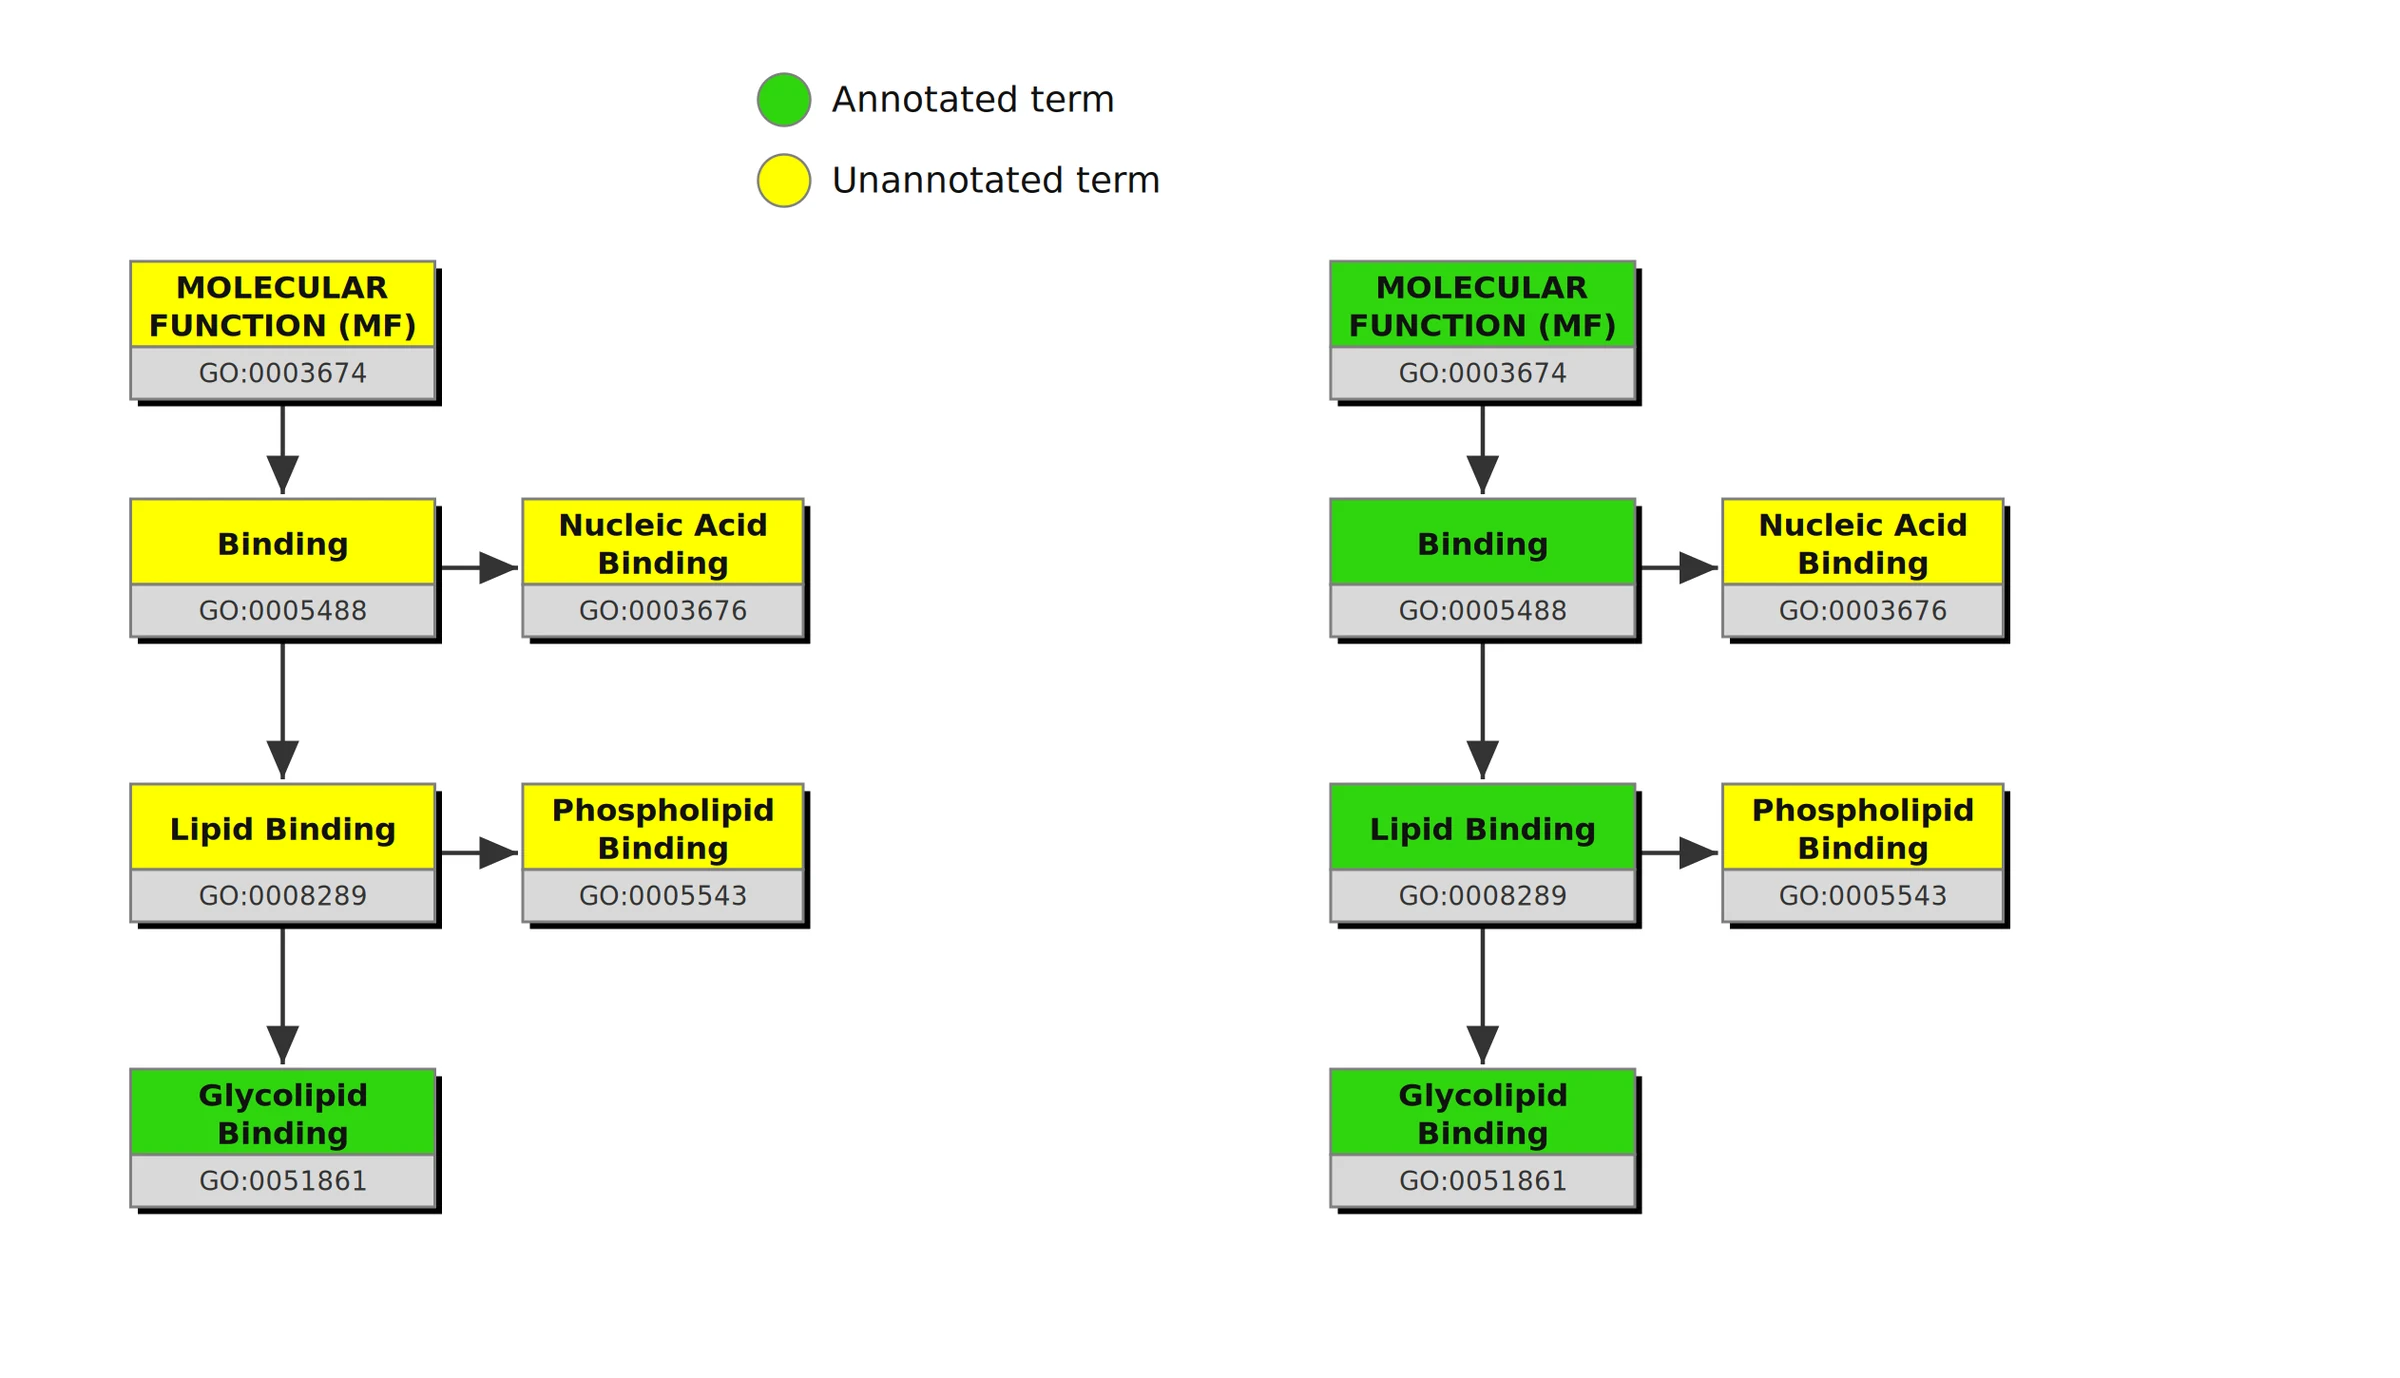
\includegraphics[width=775.3\px,height=445.2\px]{figures/fig_2_1.png}};
\fill<3>[plate] (1103.3,235) rectangle ++(387.7,445.2);
\node[tl] at (88,70) {\fmR\fz{16}{16}\color{inkii}\ls{2}\Ll{1 · Motivation}};
\node[tl] at (88,131) {\fdA\fz{54}{56.7}\color{ink}\ls{-1}\Ll{Function as a hierarchy of terms}};
\node<2-5>[tl] at (124,236) {\fbR\fz{30}{40.5}\color{ink}\Ll{Three ontologies: Biological Process\\(BP), Cellular Component (CC),\\Molecular Function (MF)}};
\node<3-5>[tl] at (124,379.5) {\fbR\fz{30}{40.5}\color{ink}\Ll{Each is a directed acyclic graph of terms\\({\fmR\fz{25.8}{31}{}is\_a}, {\fmR\fz{25.8}{31}{}part\_of})}};
\node<4-5>[tl] at (124,482.5) {\fbR\fz{30}{40.5}\color{ink}\Ll{True Path Rule: a term implies all\\its ancestors}};
\node<5>[tl] at (124,585.5) {\fbR\fz{30}{40.5}\color{ink}\Ll{Task: hierarchical multi-\\label classification}};
\node<3-5>[tl] at (694.7,718.2) {\fmR\fz{15}{19.5}\color{muted}\Ll{Dissertation, Fig. 2.1 · left inconsistent, right consistent}};
\node[tr] at (1512,876) {\fmR\fz{16}{16}\color{muted}4 / 45};
\end{tikzpicture}
\note{A protein carries many terms at different levels of specificity. If a specific term is annotated, every ancestor must be too. 

Predictions are made hierarchy-consistent before any metric is computed.}
\end{frame}

\begin{frame}[plain]
\begin{tikzpicture}[deck]
\node<1>[box] at (0,0) {\includegraphics[page=3,width=1600\px]{build/layers}};
\node<2>[box] at (0,0) {\includegraphics[page=11,width=1600\px]{build/layers}};
\node<3>[box] at (0,0) {\includegraphics[page=12,width=1600\px]{build/layers}};
\node<4>[box] at (0,0) {\includegraphics[page=13,width=1600\px]{build/layers}};
\node<2-4>[box] at (715.7,235) {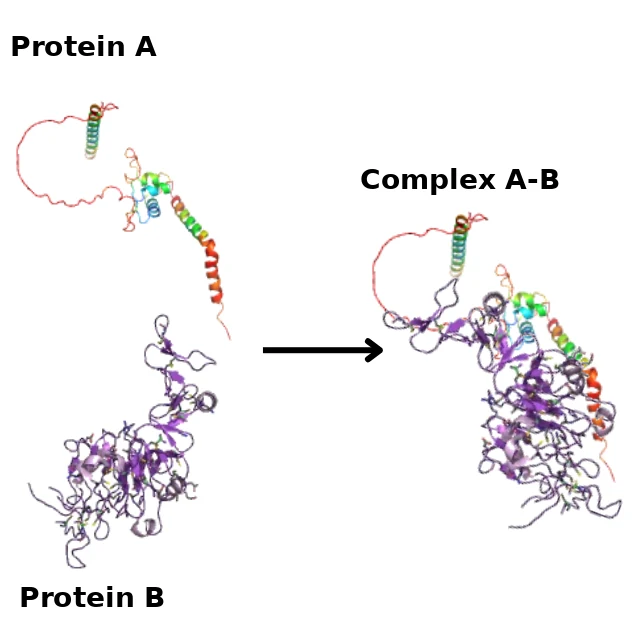
\includegraphics[width=223\px,height=223\px]{figures/fig_2_2.png}};
\node[tl] at (88,70) {\fmR\fz{16}{16}\color{inkii}\ls{2}\Ll{1 · Motivation}};
\node[tl] at (88,131) {\fdA\fz{54}{56.7}\color{ink}\ls{-1}\Ll{Function also depends on context}};
\node<2-4>[tl] at (124,236) {\fbR\fz{30}{40.5}\color{ink}\Ll{Proteins act in complexes and pathways}};
\node<2-4>[tl] at (124,298.5) {\fbR\fz{30}{40.5}\color{ink}\Ll{PPI networks: nodes are proteins, edges\\are associations}};
\node<3-4>[tl] at (124,401.5) {\fbR\fz{30}{40.5}\color{ink}\Ll{Guilt by association: connected proteins\\tend to share functions}};
\node<4>[tl] at (124,504.5) {\fbR\fz{30}{40.5}\color{ink}\Ll{But STRING mixes evidence of uneven\\reliability, and about one third of\\proteins have no edge}};
\node<2-4>[tl] at (694.7,496) {\fmR\fz{15}{19.5}\color{muted}\Ll{Dissertation, Fig. 2.2}};
\node[tr] at (1512,876) {\fmR\fz{16}{16}\color{muted}5 / 45};
\end{tikzpicture}
\note{Sequence-derived features are strong, but part of a protein's function is set by its cellular context. 

STRING aggregates experiments, curated databases, co-expression, genomic context and text mining into one confidence score. 

Coverage is uneven, which becomes the central limitation of a network-only model.}
\end{frame}

\begin{frame}[plain]
\begin{tikzpicture}[deck]
\node<1>[box] at (0,0) {\includegraphics[page=3,width=1600\px]{build/layers}};
\node<2>[box] at (0,0) {\includegraphics[page=14,width=1600\px]{build/layers}};
\node<3>[box] at (0,0) {\includegraphics[page=15,width=1600\px]{build/layers}};
\node<4>[box] at (0,0) {\includegraphics[page=16,width=1600\px]{build/layers}};
\node[tl] at (88,70) {\fmR\fz{16}{16}\color{inkii}\ls{2}\Ll{1 · Motivation}};
\node[tl] at (88,131) {\fdA\fz{54}{56.7}\color{ink}\ls{-1}\Ll{Seven research questions}};
\node<2-4>[tc] at (126,236) {\fmM\fz{20}{20}\color{ink}\Lc{RQ1}};
\node<2-4>[tl] at (184,236) {\fbR\fz{30}{39}\color{ink}\Ll{Which network representation works best?}};
\node<2-4>[tc] at (126,308) {\fmM\fz{20}{20}\color{ink}\Lc{RQ2}};
\node<2-4>[tl] at (184,308) {\fbR\fz{30}{39}\color{ink}\Ll{How much does propagating ProtT5 over\\STRING add?}};
\node<2-4>[tc] at (126,416) {\fmM\fz{20}{20}\color{ink}\Lc{RQ3}};
\node<2-4>[tl] at (184,416) {\fbR\fz{30}{39}\color{ink}\Ll{Fixed vs learned aggregation, vector vs\\image heads}};
\node<3-4>[tc] at (126,524) {\fmM\fz{20}{20}\color{ink}\Lc{RQ4}};
\node<3-4>[tl] at (184,524) {\fbR\fz{30}{39}\color{ink}\Ll{Do early and late fusion help?}};
\node<3-4>[tc] at (866,236) {\fmM\fz{20}{20}\color{ink}\Lc{RQ5}};
\node<3-4>[tl] at (924,236) {\fbR\fz{30}{39}\color{ink}\Ll{How deep, and how much retention?}};
\node<4>[tc] at (866,308) {\fmM\fz{20}{20}\color{ink}\Lc{RQ6}};
\node<4>[tl] at (924,308) {\fbR\fz{30}{39}\color{ink}\Ll{How does it compare with the literature?}};
\node<4>[tc] at (866,416) {\fmM\fz{20}{20}\color{ink}\Lc{RQ7}};
\node<4>[tl] at (924,416) {\fbR\fz{30}{39}\color{ink}\Ll{Does it work on one global, aggregated\\network?}};
\node[tr] at (1512,876) {\fmR\fz{16}{16}\color{muted}6 / 45};
\end{tikzpicture}
\note{Read the full questions from Section 1.3 only if asked. Each one is answered on the conclusions slide.}
\end{frame}

\begin{frame}[plain]
\begin{tikzpicture}[deck]
\node<1>[box] at (0,0) {\includegraphics[page=3,width=1600\px]{build/layers}};
\node<2>[box] at (0,0) {\includegraphics[page=17,width=1600\px]{build/layers}};
\node<3>[box] at (0,0) {\includegraphics[page=18,width=1600\px]{build/layers}};
\node<4>[box] at (0,0) {\includegraphics[page=19,width=1600\px]{build/layers}};
\node[tl] at (88,70) {\fmR\fz{16}{16}\color{inkii}\ls{2}\Ll{1 · Motivation}};
\node[tl] at (88,131) {\fdA\fz{54}{56.7}\color{ink}\ls{-1}\Ll{Contributions}};
\node<2-4>[tl] at (144,237) {\fbR\fz{32}{41.6}\color{ink}\Ll{NEXUS-GO: non-parametric multi-hop propagation of ProtT5 embeddings over STRING}};
\node<2-4>[tl] at (144,304.6) {\fbR\fz{32}{41.6}\color{ink}\Ll{Controlled comparison of fixed vs learned (GCN, GAT) aggregation}};
\node<2-4>[tl] at (144,372.2) {\fbR\fz{32}{41.6}\color{ink}\Ll{Vector vs image classification heads over the same embeddings}};
\node<3-4>[tl] at (144,439.8) {\fbR\fz{32}{41.6}\color{ink}\Ll{Early and late fusion of fixed and learned routes}};
\node<3-4>[tl] at (144,507.4) {\fbR\fz{32}{41.6}\color{ink}\Ll{Benchmark against five reimplemented methods, same splits and setting}};
\node<4>[tl] at (88,768.7) {\fmM\fz{18}{21.6}\color{ink}\Ll{VISAPP 2026 · published, pp. 157–166}};
\node<4>[tl] at (88,800.3) {\fbR\fz{21}{28.4}\color{inkii}\Ll{{\fbI\color{ink}{}From Graphs to Images: Non-Parametric PPI Context Integration for}\\{\fbI\color{ink}{}Vision-Based Protein Function Prediction}}};
\node<4>[tl] at (824,768.7) {\fmM\fz{18}{21.6}\color{ink}\Ll{CCIS · accepted, expected December 2026}};
\node<4>[tl] at (824,800.3) {\fbR\fz{21}{28.4}\color{inkii}\Ll{{\fbI\color{ink}{}Beyond Learnable Graphs: Fixed Multi-Hop PPI Diffusion of Sequence}\\{\fbI\color{ink}{}Embeddings for Robust Protein Function Prediction} · extended version}};
\node[tr] at (1512,876) {\fmR\fz{16}{16}\color{muted}7 / 45};
\end{tikzpicture}
\note{Five contributions, each answered with a result at the end. 

The first paper reported the first, sum-deduplicated campaign; the extended version continues the fixed route and adds a vector head next to the vision head. It was accepted in Communications in Computer and Information Science.}
\end{frame}

\section{2 · Background and related work}
\begin{frame}[plain]
\begin{tikzpicture}[deck]
\node<1>[box] at (0,0) {\includegraphics[page=3,width=1600\px]{build/layers}};
\node<2>[box] at (0,0) {\includegraphics[page=20,width=1600\px]{build/layers}};
\node<3>[box] at (0,0) {\includegraphics[page=21,width=1600\px]{build/layers}};
\node<4>[box] at (0,0) {\includegraphics[page=22,width=1600\px]{build/layers}};
\node<5>[box] at (0,0) {\includegraphics[page=23,width=1600\px]{build/layers}};
\node<2-5>[box] at (123.6,235) {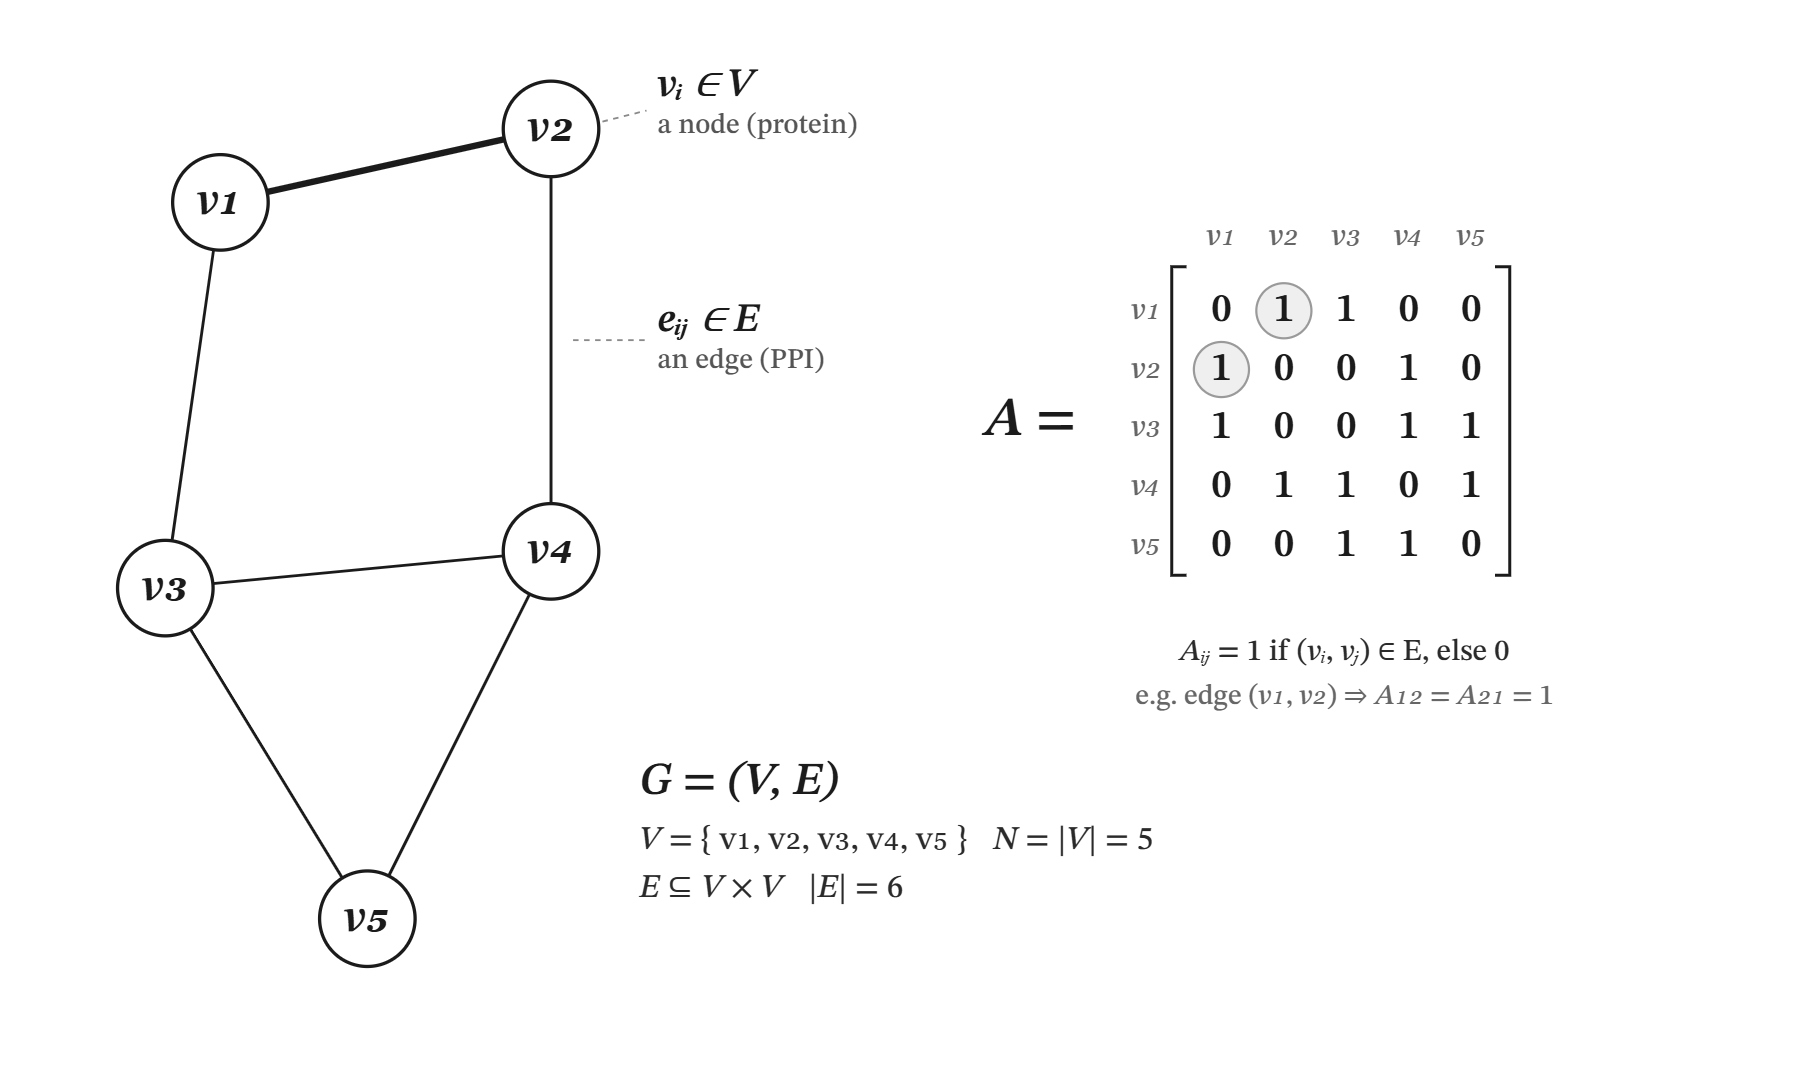
\includegraphics[width=624.8\px,height=370\px]{figures/fig_2_3.png}};
\node[tl] at (88,70) {\fmR\fz{16}{16}\color{inkii}\ls{2}\Ll{2 · Background and related work}};
\node[tl] at (88,131) {\fdA\fz{54}{56.7}\color{ink}\ls{-1}\Ll{Graphs, adjacency and message passing}};
\node<2-5>[tl] at (88,643) {\fmR\fz{15}{19.5}\color{muted}\Ll{Dissertation, Fig. 2.3}};
\node<2-5>[tl] at (124,689) {\fbR\fz{26}{35.1}\color{ink}\Ll{{\fz{29.2}{35}$G = (V, E, w)$}: proteins, associations,\\STRING confidence}};
\node<3-5>[tl] at (852,689) {\fbR\fz{26}{35.1}\color{ink}\Ll{Message passing: aggregate neighbours, update\\the node}};
\node<2-5>[tl] at (124,775.2) {\fbR\fz{26}{35.1}\color{ink}\Ll{Adjacency matrix {\fz{29.2}{35}$A$}; sparse storage {\fz{29.2}{35}$O(|E|)$}}};
\node<5>[tl] at (852,775.2) {\fbR\fz{26}{35.1}\color{ink}\Ll{{\fz{29.2}{35}$L$} layers reach {\fz{29.2}{35}$L$} hops; too many cause oversmoothing}};
\node[tr] at (1512,876) {\fmR\fz{16}{16}\color{muted}8 / 45};
\end{tikzpicture}
\note{GCN aggregates with a symmetrically normalized adjacency; GAT learns attention weights over neighbours. 

Each layer widens the receptive field by one hop, and too many layers make neighbouring representations indistinguishable.}
\end{frame}

\begin{frame}[plain]
\begin{tikzpicture}[deck]
\node<1>[box] at (0,0) {\includegraphics[page=3,width=1600\px]{build/layers}};
\node<2>[box] at (0,0) {\includegraphics[page=24,width=1600\px]{build/layers}};
\node<3>[box] at (0,0) {\includegraphics[page=25,width=1600\px]{build/layers}};
\node<4>[box] at (0,0) {\includegraphics[page=26,width=1600\px]{build/layers}};
\node<3-4>[box] at (594.3,440) {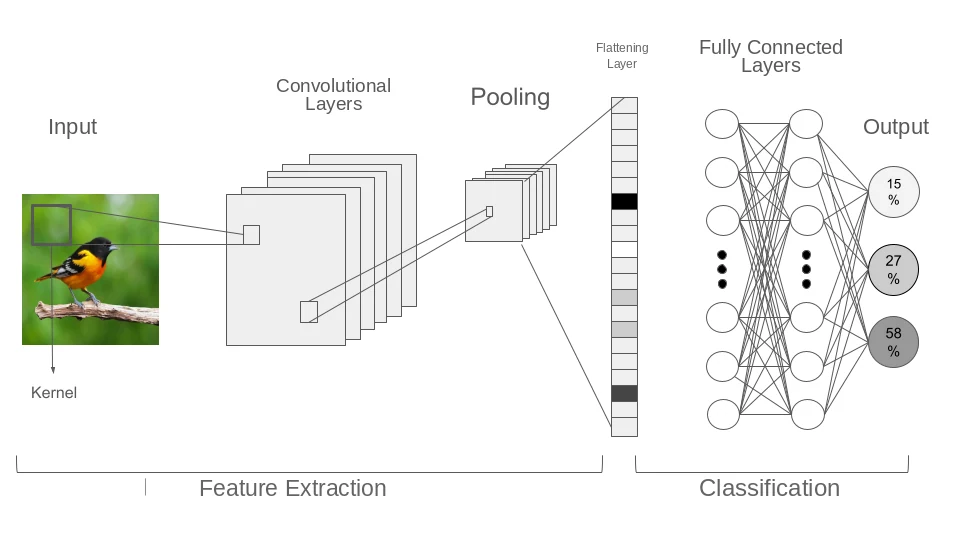
\includegraphics[width=411.3\px,height=231.4\px]{figures/fig_2_6.png}};
\node<4>[box] at (1079.7,435.7) {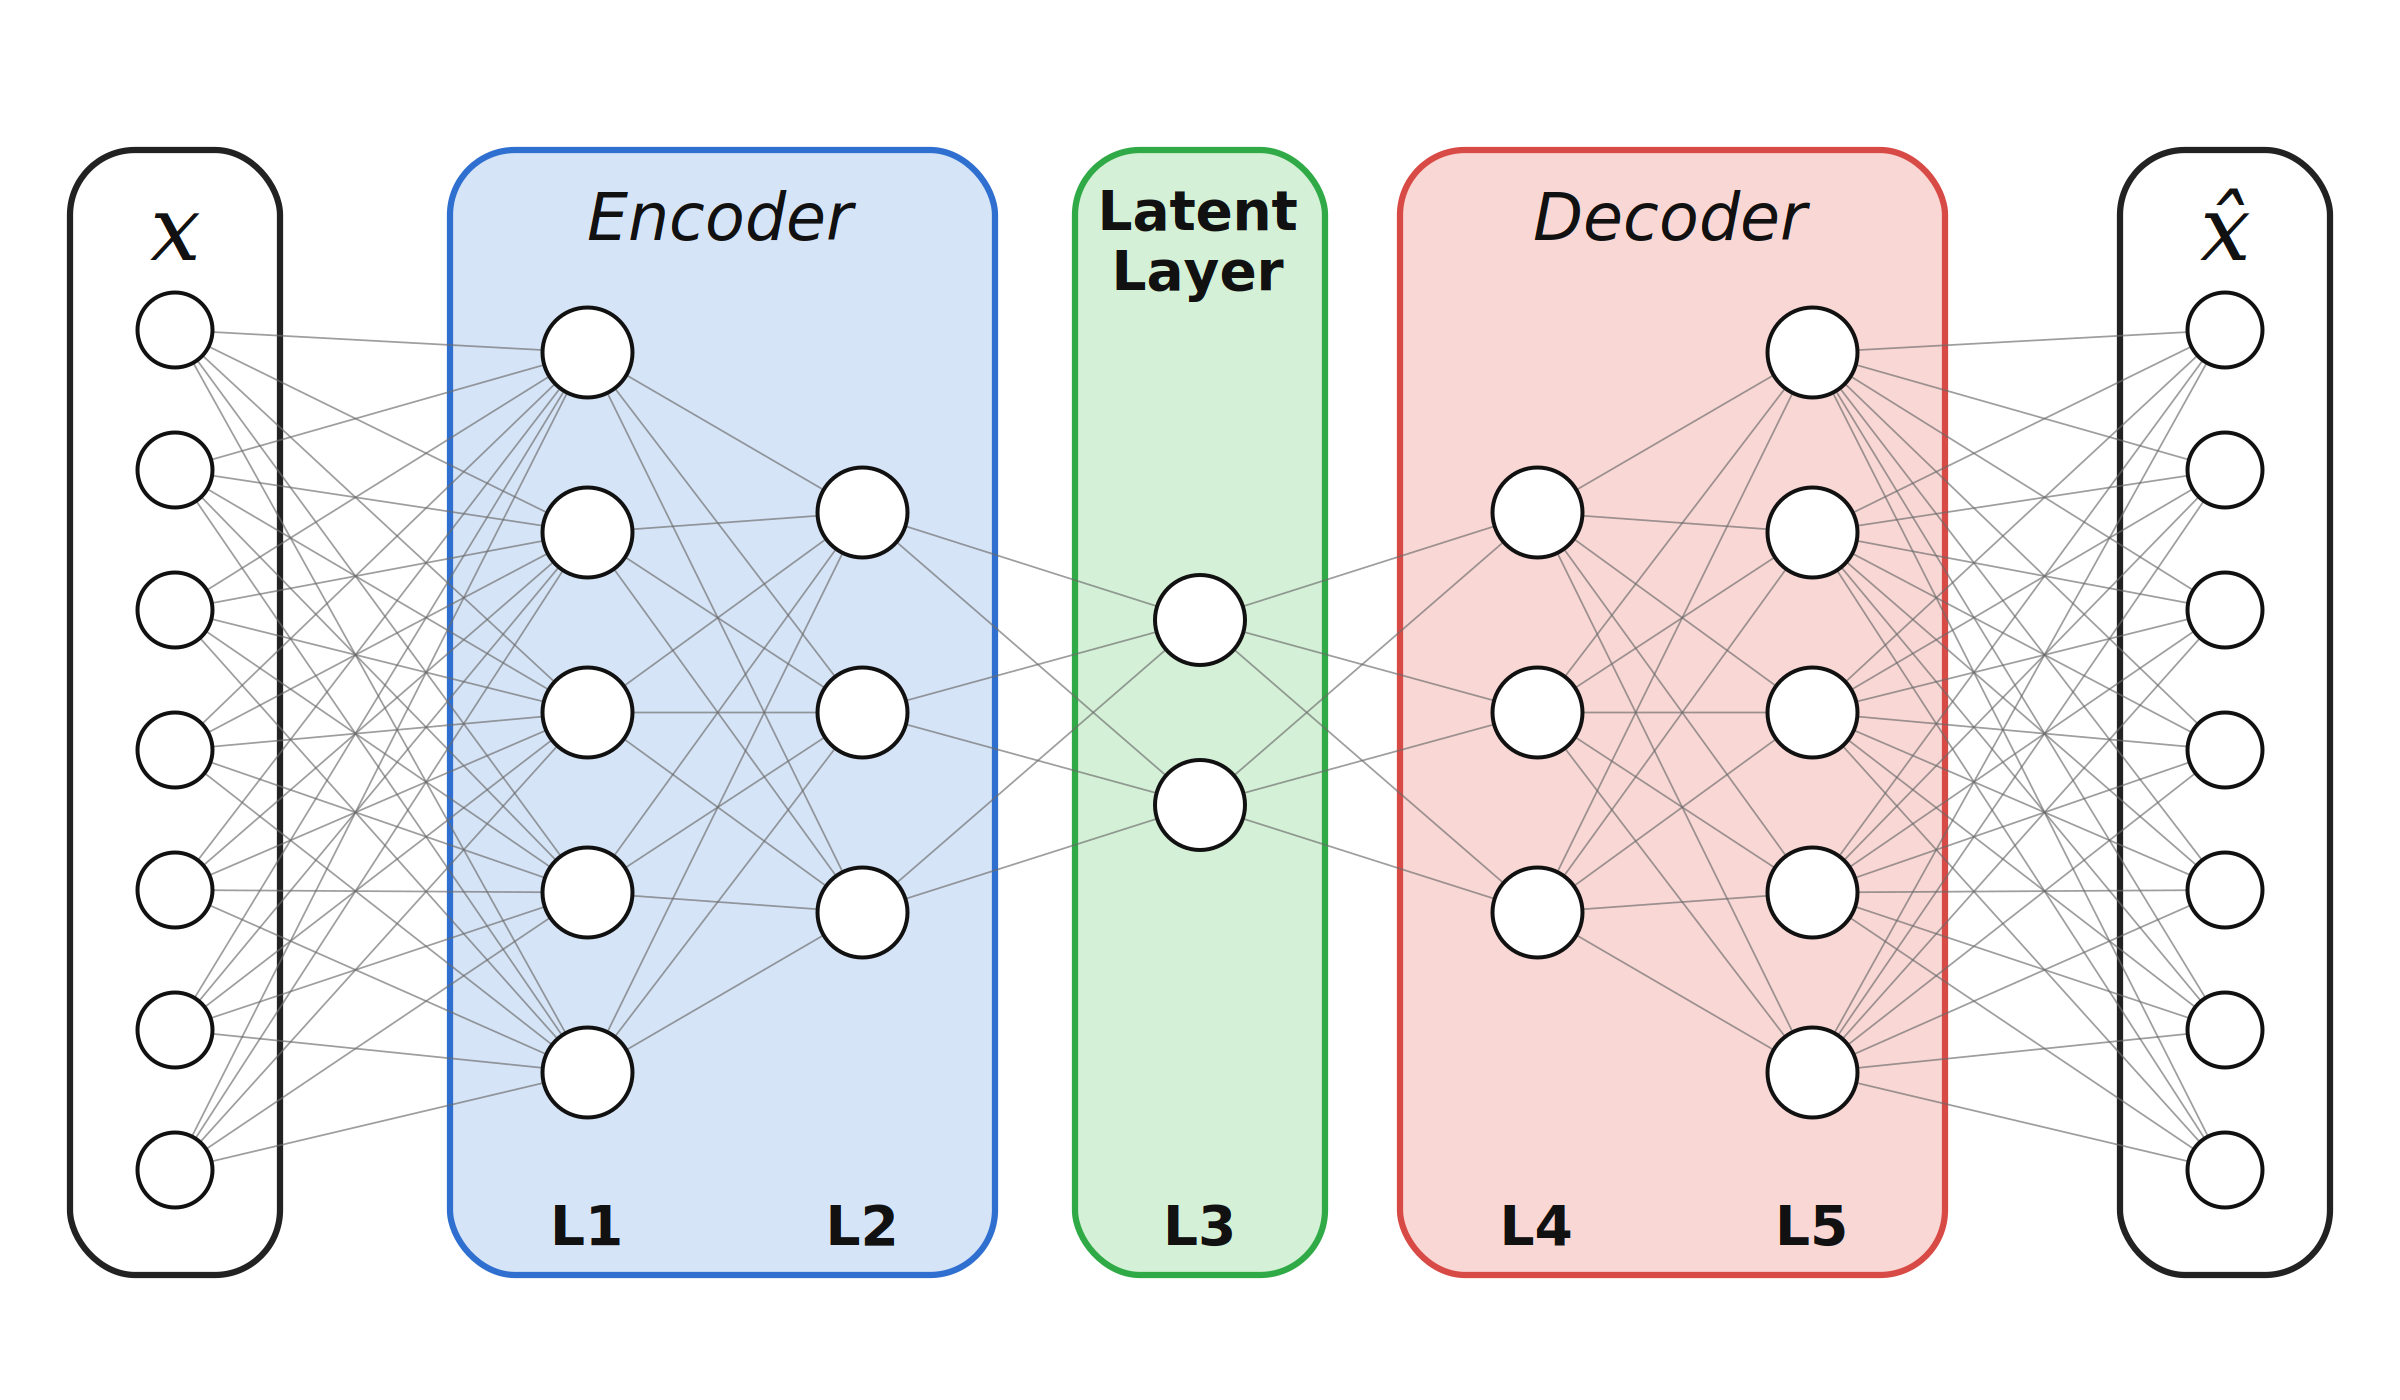
\includegraphics[width=411.3\px,height=239.9\px]{figures/fig_2_7.png}};
\node[tl] at (88,70) {\fmR\fz{16}{16}\color{inkii}\ls{2}\Ll{2 · Background and related work}};
\node[tl] at (88,131) {\fdA\fz{54}{56.7}\color{ink}\ls{-1}\Ll{Building blocks}};
\node<2-4>[tl] at (88,230) {\fbR\fz{24}{32.4}\color{ink}\Ll{{\fbB{}MLP}: the vector prediction head}};
\node<3-4>[tl] at (573.3,230) {\fbR\fz{24}{32.4}\color{ink}\Ll{{\fbB{}CNN}: the backbone of the image route\\(ResNet-50, ConvNeXt-Tiny)}};
\node<4>[tl] at (1058.7,230) {\fbR\fz{24}{32.4}\color{ink}\Ll{{\fbB{}Autoencoder}: the compression inside\\deepNF, one of the baselines}};
\node<2-4>[tl] at (88,854.9) {\fmR\fz{15}{19.5}\color{muted}\Ll{Dissertation, Figs. 2.4 and 2.5}};
\node<3-4>[tl] at (573.3,831.5) {\fmR\fz{15}{19.5}\color{muted}\Ll{Dissertation, Fig. 2.6}};
\node<4>[tl] at (1058.7,831.5) {\fmR\fz{15}{19.5}\color{muted}\Ll{Dissertation, Fig. 2.7}};
\node[tr] at (1512,876) {\fmR\fz{16}{16}\color{muted}9 / 45};
\end{tikzpicture}
\note{Only what the rest of the talk needs. 

The MLP is the vector head, the CNN is the vision head, and the autoencoder is how deepNF compresses diffusion states.}
\end{frame}

\begin{frame}[plain]
\begin{tikzpicture}[deck]
\node<1>[box] at (0,0) {\includegraphics[page=3,width=1600\px]{build/layers}};
\node<2>[box] at (0,0) {\includegraphics[page=27,width=1600\px]{build/layers}};
\node<3>[box] at (0,0) {\includegraphics[page=28,width=1600\px]{build/layers}};
\node<4>[box] at (0,0) {\includegraphics[page=29,width=1600\px]{build/layers}};
\node<5>[box] at (0,0) {\includegraphics[page=30,width=1600\px]{build/layers}};
\node[tl] at (88,70) {\fmR\fz{16}{16}\color{inkii}\ls{2}\Ll{2 · Background and related work}};
\node[tl] at (88,131) {\fdA\fz{54}{56.7}\color{ink}\ls{-1}\Ll{Protein language models}};
\node<2-5>[tl] at (124,236) {\fbR\fz{30}{40.5}\color{ink}\Ll{Self-supervised pretraining on hundreds\\of millions of sequences}};
\node<3-5>[tl] at (124,339) {\fbR\fz{30}{40.5}\color{ink}\Ll{Transformer encoder: every residue\\attends to every other}};
\node<4-5>[tl] at (124,442) {\fbR\fz{30}{40.5}\color{ink}\Ll{ProtT5-XL-U50: T5 encoder, BFD then\\UniRef50, 15\% residue masking}};
\node<5>[tl] at (124,545) {\fbR\fz{30}{40.5}\color{ink}\Ll{Used here as a frozen feature extractor}};
\node[tr] at (1512,876) {\fmR\fz{16}{16}\color{muted}10 / 45};
\end{tikzpicture}
\note{Language models turn function prediction into ordinary multi-label classification over a fixed-length vector. 

No gradient from our task reaches ProtT5; we read three encoder layers and keep them fixed.}
\end{frame}

\begin{frame}[plain]
\begin{tikzpicture}[deck]
\node<1>[box] at (0,0) {\includegraphics[page=3,width=1600\px]{build/layers}};
\node<2>[box] at (0,0) {\includegraphics[page=31,width=1600\px]{build/layers}};
\node<3>[box] at (0,0) {\includegraphics[page=32,width=1600\px]{build/layers}};
\node<4>[box] at (0,0) {\includegraphics[page=33,width=1600\px]{build/layers}};
\node[tl] at (88,70) {\fmR\fz{16}{16}\color{inkii}\ls{2}\Ll{2 · Background and related work}};
\node[tl] at (88,131) {\fdA\fz{54}{56.7}\color{ink}\ls{-1}\Ll{From neighbour voting to graph transformers}};
\node[tr] at (1512,876) {\fmR\fz{16}{16}\color{muted}11 / 45};
\end{tikzpicture}
\note{The field moved from fixed diffusion to learned attention, and each step added parameters. 

Decoupled methods such as SGC and APPNP move against that trend, and SEGT-GO's multi-hop aggregation is itself a plain matrix product.}
\end{frame}

\begin{frame}[plain]
\begin{tikzpicture}[deck]
\node<1-2>[box] at (0,0) {\includegraphics[page=3,width=1600\px]{build/layers}};
\node<3>[box] at (0,0) {\includegraphics[page=34,width=1600\px]{build/layers}};
\node<4>[box] at (0,0) {\includegraphics[page=35,width=1600\px]{build/layers}};
\node<5>[box] at (0,0) {\includegraphics[page=36,width=1600\px]{build/layers}};
\node[tl] at (88,70) {\fmR\fz{16}{16}\color{inkii}\ls{2}\Ll{2 · Background and related work}};
\node[tl] at (88,131) {\fdA\fz{54}{56.7}\color{ink}\ls{-1}\Ll{The open question}};
\node<2-5>[tl] at (88,262) {\fdA\fz{64}{69.1}\color{ink}\ls{-1.5}\Ll{Is a learned graph component still needed\\once the propagated object is informative?}};
\node<3-5>[tl] at (124,426.2) {\fbR\fz{30}{40.5}\color{ink}\Ll{Proposal: propagate ProtT5 embeddings with a fixed, finite-step operator, then use an\\ordinary head}};
\node<4-5>[tl] at (124,529.2) {\fbR\fz{30}{40.5}\color{ink}\Ll{A sequence representation exists for every protein, so the network adds instead\\of supplies}};
\node<5>[tl] at (124,632.2) {\fbR\fz{30}{40.5}\color{ink}\Ll{No prior visual route starts from a propagated language-model embedding}};
\node[tr] at (1512,876) {\fmR\fz{16}{16}\color{muted}12 / 45};
\end{tikzpicture}
\note{The contribution is an architectural placement, not a new propagation mechanism. 

To our knowledge no previous work propagates protein language model embeddings directly while simplifying what consumes them.}
\end{frame}

\section{3 · Data and evaluation}
\begin{frame}[plain]
\begin{tikzpicture}[deck]
\node<1>[box] at (0,0) {\includegraphics[page=3,width=1600\px]{build/layers}};
\node<2>[box] at (0,0) {\includegraphics[page=37,width=1600\px]{build/layers}};
\node<3>[box] at (0,0) {\includegraphics[page=38,width=1600\px]{build/layers}};
\node<4>[box] at (0,0) {\includegraphics[page=39,width=1600\px]{build/layers}};
\node[tl] at (88,70) {\fmR\fz{16}{16}\color{inkii}\ls{2}\Ll{3 · Data and evaluation}};
\node[tl] at (88,131) {\fdA\fz{54}{56.7}\color{ink}\ls{-1}\Ll{Data: a CAFA5-derived corpus}};
\node<2-4>[tl] at (106,237) {\fbB\fz{20}{24}\color{inkii}\Ll{Ontology}};
\node<2-4>[tr] at (547.6,237) {\fbB\fz{20}{24}\color{inkii}\Lr{Training}};
\node<2-4>[tr] at (677.8,237) {\fbB\fz{20}{24}\color{inkii}\Lr{Validation}};
\node<2-4>[tr] at (797.8,237) {\fbB\fz{20}{24}\color{inkii}\Lr{Test}};
\node<2-4>[tr] at (891.1,237) {\fbB\fz{20}{24}\color{inkii}\Lr{Terms}};
\node<2-4>[tl] at (106,295) {\fbR\fz{28}{33.6}\color{ink}\Ll{Biological Process (BP)}};
\node<2-4>[tr] at (547.6,296) {\fmR\fz{28}{33.6}\color{ink}\Lr{73,768}};
\node<2-4>[tr] at (677.8,296) {\fmR\fz{28}{33.6}\color{ink}\Lr{9,221}};
\node<2-4>[tr] at (797.8,296) {\fmR\fz{28}{33.6}\color{ink}\Lr{9,221}};
\node<2-4>[tr] at (891.1,296) {\fmR\fz{28}{33.6}\color{ink}\Lr{500}};
\node<2-4>[tl] at (106,357) {\fbR\fz{28}{33.6}\color{ink}\Ll{Cellular Component (CC)}};
\node<2-4>[tr] at (547.6,358) {\fmR\fz{28}{33.6}\color{ink}\Lr{74,328}};
\node<2-4>[tr] at (677.8,358) {\fmR\fz{28}{33.6}\color{ink}\Lr{9,292}};
\node<2-4>[tr] at (797.8,358) {\fmR\fz{28}{33.6}\color{ink}\Lr{9,292}};
\node<2-4>[tr] at (891.1,358) {\fmR\fz{28}{33.6}\color{ink}\Lr{498}};
\node<2-4>[tl] at (106,419) {\fbR\fz{28}{33.6}\color{ink}\Ll{Molecular Function (MF)}};
\node<2-4>[tr] at (547.6,420) {\fmR\fz{28}{33.6}\color{ink}\Lr{62,909}};
\node<2-4>[tr] at (677.8,420) {\fmR\fz{28}{33.6}\color{ink}\Lr{7,864}};
\node<2-4>[tr] at (797.8,420) {\fmR\fz{28}{33.6}\color{ink}\Lr{7,864}};
\node<2-4>[tr] at (891.1,420) {\fmR\fz{28}{33.6}\color{ink}\Lr{499}};
\node<2-4>[tl] at (88,466) {\fmR\fz{15}{19.5}\color{muted}\Ll{Dissertation, Table 4.1}};
\node<3-4>[tl] at (973.3,236) {\fbR\fz{30}{40.5}\color{ink}\Ll{80 / 10 / 10 split, disjoint at\\protein level, no temporal or\\homology constraint}};
\node<4>[tl] at (973.3,379.5) {\fbR\fz{30}{40.5}\color{ink}\Ll{Labels per protein (mean): 25.91 BP,\\12.48 CC, 7.55 MF}};
\node<4>[tl] at (973.3,482.5) {\fbR\fz{30}{40.5}\color{ink}\Ll{Label matrix density:}};
\node<4>[tl] at (973.3,526) {\fmR\fz{22}{29.7}\color{inkii}\Ll{BP}};
\node<4>[tl] at (1164,526) {\fmR\fz{22}{29.7}\color{ink}\Ll{5.18\%}};
\node<4>[tl] at (973.3,565.7) {\fmR\fz{22}{29.7}\color{inkii}\Ll{CC}};
\node<4>[tl] at (1094.6,565.7) {\fmR\fz{22}{29.7}\color{ink}\Ll{2.51\%}};
\node<4>[tl] at (973.3,605.4) {\fmR\fz{22}{29.7}\color{inkii}\Ll{MF}};
\node<4>[tl] at (1068.6,605.4) {\fmR\fz{22}{29.7}\color{ink}\Ll{1.51\%}};
\node[tr] at (1512,876) {\fmR\fz{16}{16}\color{muted}13 / 45};
\end{tikzpicture}
\note{The official CAFA5 test labels were not available, so the splits come from the training corpus. 

Only about five hundred most frequent terms per ontology are kept, which makes absolute values not comparable with CAFA numbers.}
\end{frame}

\begin{frame}[plain]
\begin{tikzpicture}[deck]
\node<1>[box] at (0,0) {\includegraphics[page=3,width=1600\px]{build/layers}};
\node<2>[box] at (0,0) {\includegraphics[page=40,width=1600\px]{build/layers}};
\node<3>[box] at (0,0) {\includegraphics[page=41,width=1600\px]{build/layers}};
\node<4>[box] at (0,0) {\includegraphics[page=42,width=1600\px]{build/layers}};
\node<2-4>[box] at (109,235) {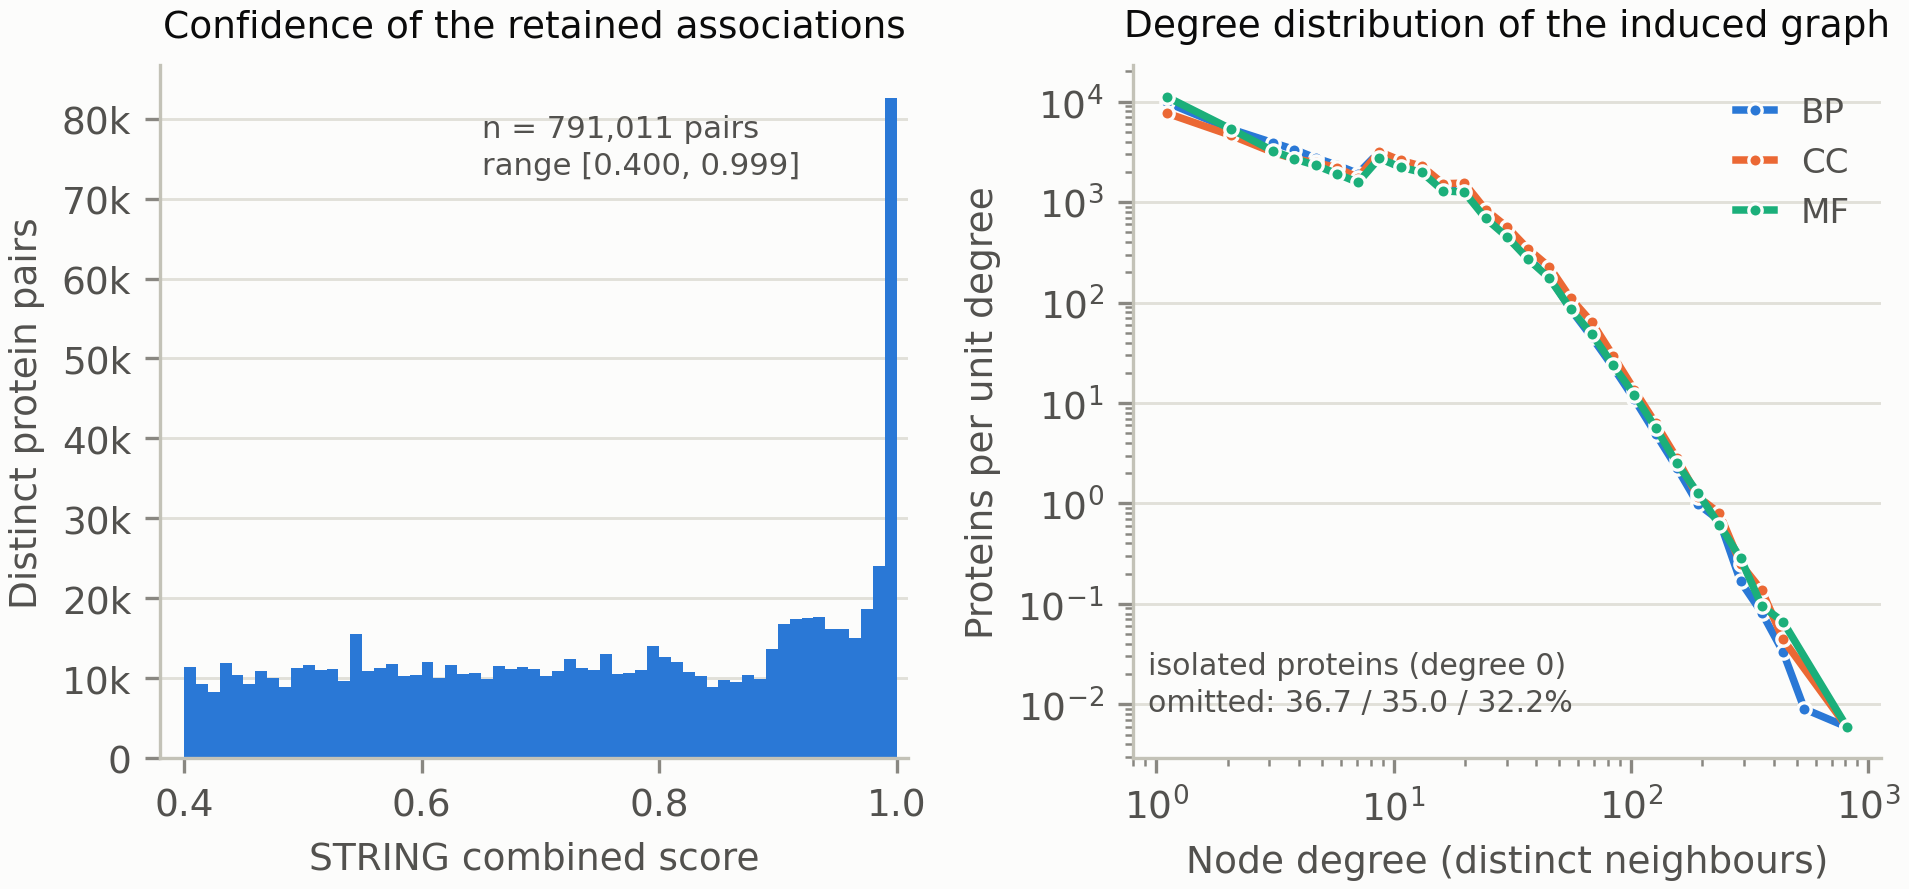
\includegraphics[width=775.3\px,height=361\px]{figures/fig_4_1.png}};
\fill<2-3>[plate] (496.7,235) rectangle ++(387.7,361);
\node[tl] at (88,70) {\fmR\fz{16}{16}\color{inkii}\ls{2}\Ll{3 · Data and evaluation}};
\node[tl] at (88,131) {\fdA\fz{54}{56.7}\color{ink}\ls{-1}\Ll{STRING v11.5: one aggregated network}};
\node<2-4>[tl] at (88,634) {\fmR\fz{15}{19.5}\color{muted}\Ll{Dissertation, Fig. 4.1 · left combined score, right degree}};
\node<2-4>[tl] at (973.3,232) {\fbR\fz{26}{35.1}\color{ink}\Ll{2,422,234 records, 791,011 distinct pairs,\\86,423 proteins}};
\node<2-4>[tl] at (973.3,318.2) {\fbR\fz{26}{35.1}\color{ink}\Ll{Combined score in [0.400, 0.999]; confidence,\\not binding strength}};
\node<3-4>[tl] at (973.3,404.4) {\fbR\fz{26}{35.1}\color{ink}\Ll{Each pair repeated 3.06 times on average (up\\to 170), always with the same score}};
\node<4>[tl] at (973.3,490.6) {\fbR\fz{26}{35.1}\color{ink}\Ll{Degree is heavy-tailed: median 5 to 7,\\maximum 763 to 805}};
\node[tr] at (1512,876) {\fmR\fz{16}{16}\color{muted}14 / 45};
\end{tikzpicture}
\note{The medium-confidence floor of 400 comes with the inherited file. 

Repeated records carry no extra score information, which later decides the deduplication rule. Some knowledge circularity with the annotations cannot be excluded.}
\end{frame}

\begin{frame}[plain]
\begin{tikzpicture}[deck]
\node<1>[box] at (0,0) {\includegraphics[page=3,width=1600\px]{build/layers}};
\node<2>[box] at (0,0) {\includegraphics[page=43,width=1600\px]{build/layers}};
\node<3>[box] at (0,0) {\includegraphics[page=44,width=1600\px]{build/layers}};
\node<2-3>[box] at (109,235.6) {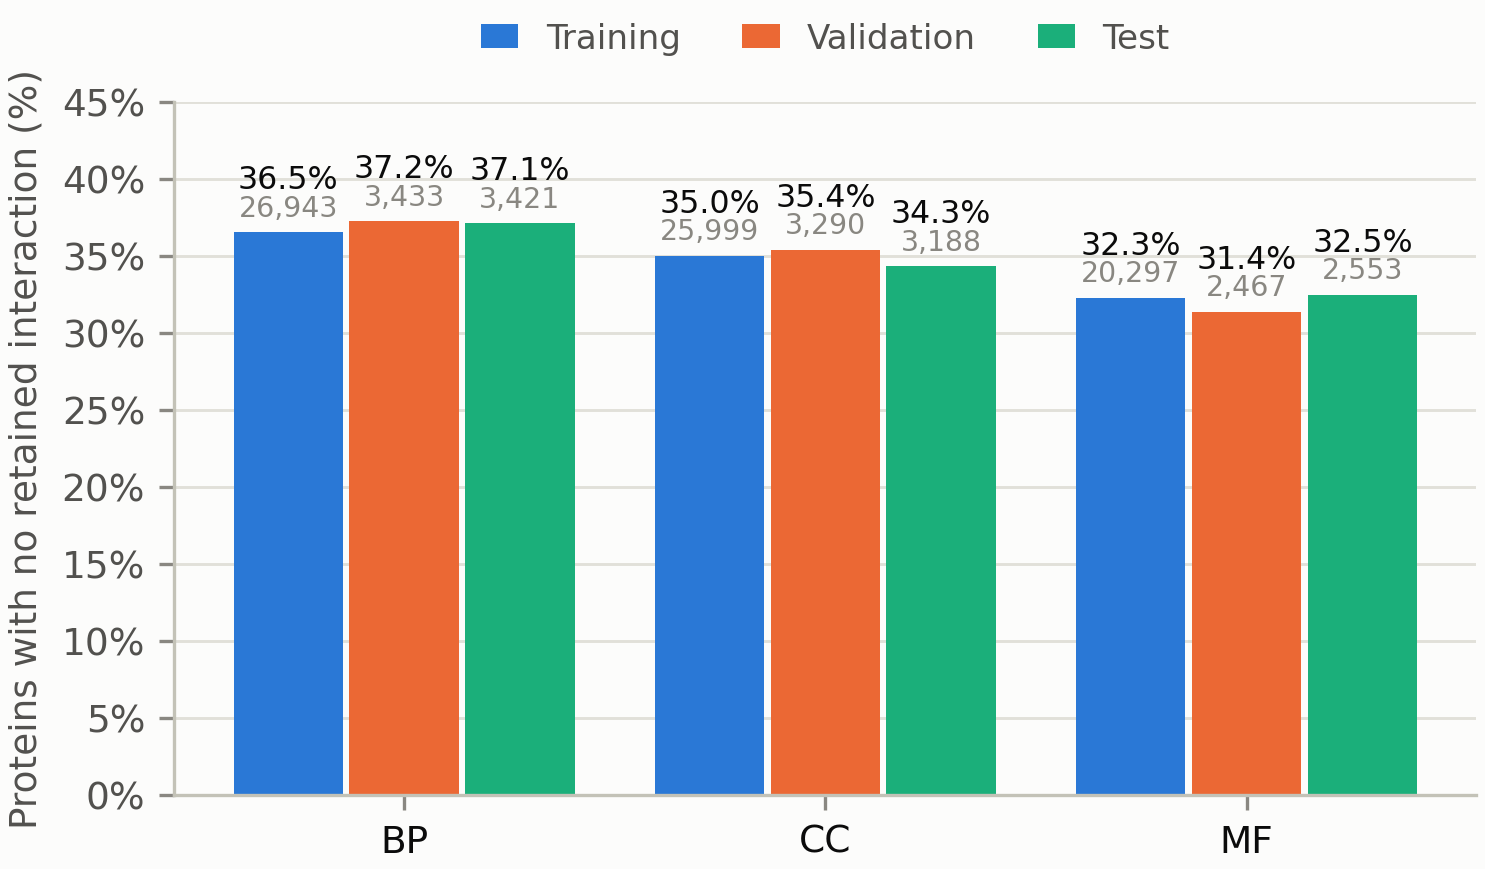
\includegraphics[width=654\px,height=382.7\px]{figures/fig_4_2.png}};
\node<3>[box] at (843.3,235) {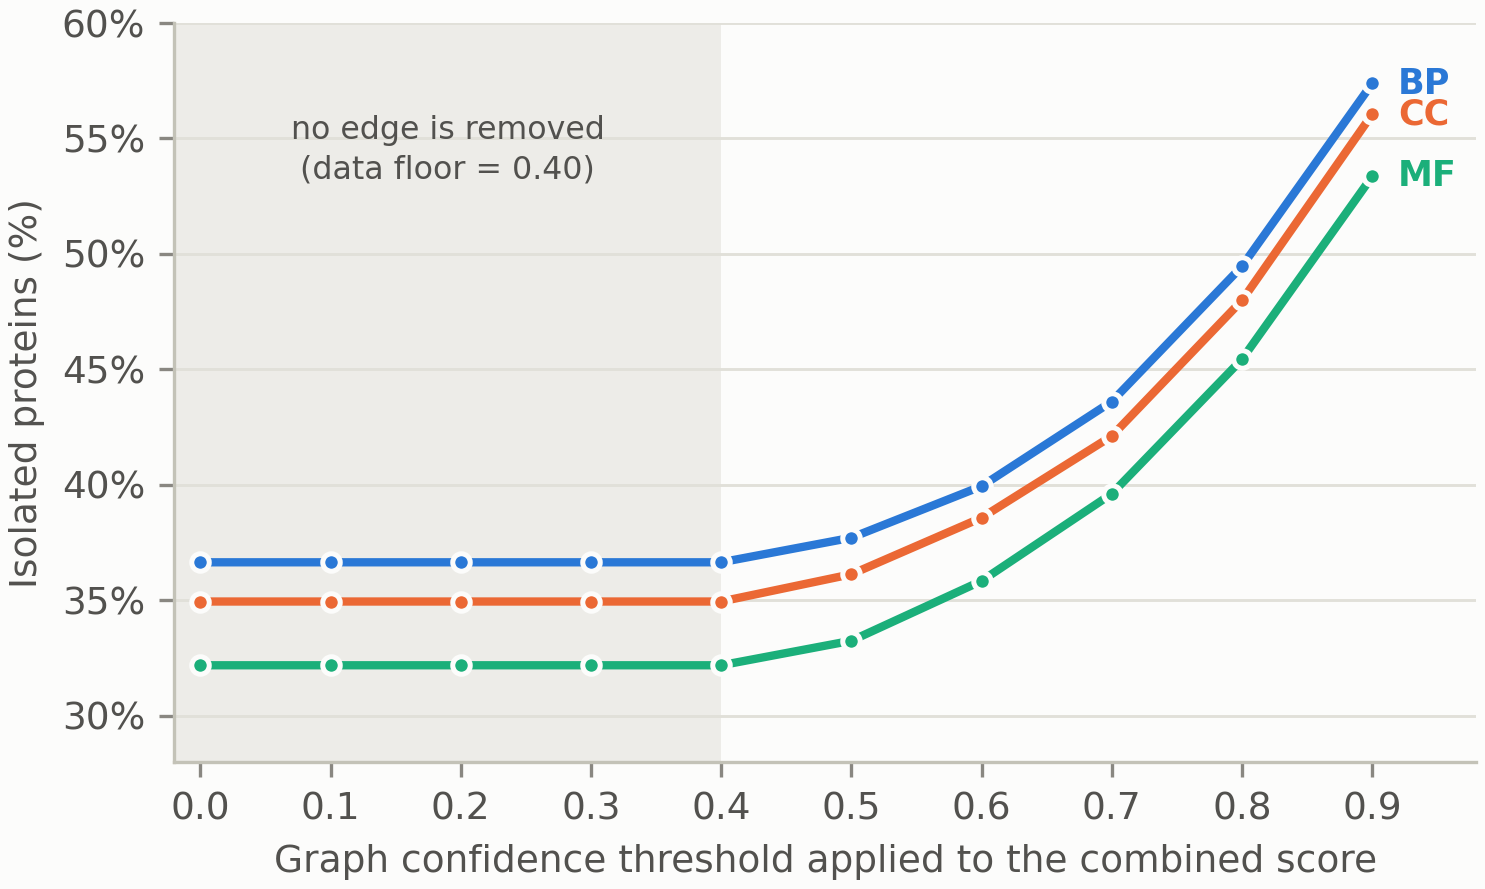
\includegraphics[width=641.4\px,height=384\px]{figures/fig_4_3.png}};
\node[tl] at (88,70) {\fmR\fz{16}{16}\color{inkii}\ls{2}\Ll{3 · Data and evaluation}};
\node[tl] at (88,131) {\fdA\fz{54}{56.7}\color{ink}\ls{-1}\Ll{One third of the proteins have no edge}};
\node<2-3>[tl] at (88,657) {\fmR\fz{15}{19.5}\color{muted}\Ll{Dissertation, Fig. 4.2}};
\node<2-3>[tl] at (124,719.5) {\fbR\fz{30}{40.5}\color{ink}\Ll{Isolated: 36.65\% BP, 34.95\% CC, 32.19\% MF}};
\node<2-3>[tl] at (124,782) {\fbR\fz{30}{40.5}\color{ink}\Ll{Stable across training, validation and test}};
\node<3>[tl] at (816,657) {\fmR\fz{15}{19.5}\color{muted}\Ll{Dissertation, Fig. 4.3}};
\node<3>[tl] at (852,719.5) {\fbR\fz{30}{40.5}\color{ink}\Ll{Thresholds up to 0.40 are inert; at 0.90 more\\than half the proteins are isolated}};
\node[tr] at (1512,876) {\fmR\fz{16}{16}\color{muted}15 / 45};
\end{tikzpicture}
\note{Isolated proteins were kept as nodes so that every protein is scored. For a model that sees only the network, these proteins have no input at all. 

This is the limitation the second generation is built to remove.}
\end{frame}

\begin{frame}[plain]
\begin{tikzpicture}[deck]
\node<1>[box] at (0,0) {\includegraphics[page=3,width=1600\px]{build/layers}};
\node<2>[box] at (0,0) {\includegraphics[page=7,width=1600\px]{build/layers}};
\node<3>[box] at (0,0) {\includegraphics[page=45,width=1600\px]{build/layers}};
\node<4>[box] at (0,0) {\includegraphics[page=46,width=1600\px]{build/layers}};
\node[tl] at (88,70) {\fmR\fz{16}{16}\color{inkii}\ls{2}\Ll{3 · Data and evaluation}};
\node[tl] at (88,131) {\fdA\fz{54}{56.7}\color{ink}\ls{-1}\Ll{Six protein-centric metrics}};
\node<2-4>[tl] at (124,236) {\fbR\fz{30}{40.5}\color{ink}\Ll{Primary criterion: wF\textsubscript{max}, information-\\content weighted}};
\node<3-4>[tl] at (124,339) {\fbR\fz{30}{40.5}\color{ink}\Ll{Also F\textsubscript{max}, F*\textsubscript{max} (root excluded), S\textsubscript{min}\\(bits, lower is better), AuPRC, IAuPRC}};
\node<4>[tl] at (124,442) {\fbR\fz{30}{40.5}\color{ink}\Ll{Predictions made hierarchy-consistent\\before scoring}};
\node<4>[tl] at (124,545) {\fbR\fz{30}{40.5}\color{ink}\Ll{101 thresholds; full evaluation mode\\(unpredicted proteins count as\\zero recall)}};
\node<2-4>[tl] at (694.7,261.7) {\fbR\fz{34}{40.8}\color{ink}\Ll{{\fz{38.2}{45.8}$\displaystyle wF_{\max} = \max_{\tau}\, \frac{2 \cdot wpr(\tau) \cdot wrc(\tau)}{wpr(\tau) + wrc(\tau)}$}}};
\node<2-4>[tl] at (694.7,341.4) {\fbR\fz{24}{32.4}\color{inkii}\Ll{each term weighted by its information content, {\fz{26.9}{32.3}$\mathrm{IC}(v) = -\log_2 \widehat{P}\bigl(v \mid \mathrm{pa}(v)\bigr)$}}};
\node<4>[tl] at (694.7,409.5) {\fbR\fz{34}{40.8}\color{ink}\Ll{{\fz{38.2}{45.8}$\displaystyle \tilde{s}_{iv} = \max_{u \in \mathcal{D}(v)} s_{iu}$}}};
\node[tr] at (1512,876) {\fmR\fz{16}{16}\color{muted}16 / 45};
\end{tikzpicture}
\note{wF\textsubscript{max} weights each term by information content, so frequent terms near the root count little. It is the selection criterion everywhere. 

The ancestor closure of predictions uses \texttt{is\_a} only, which matters most for CC.}
\end{frame}

\begin{frame}[plain]
\begin{tikzpicture}[deck]
\node<1>[box] at (0,0) {\includegraphics[page=3,width=1600\px]{build/layers}};
\node<2>[box] at (0,0) {\includegraphics[page=47,width=1600\px]{build/layers}};
\node<3>[box] at (0,0) {\includegraphics[page=48,width=1600\px]{build/layers}};
\node<4>[box] at (0,0) {\includegraphics[page=49,width=1600\px]{build/layers}};
\node<2-4>[box] at (109,235) {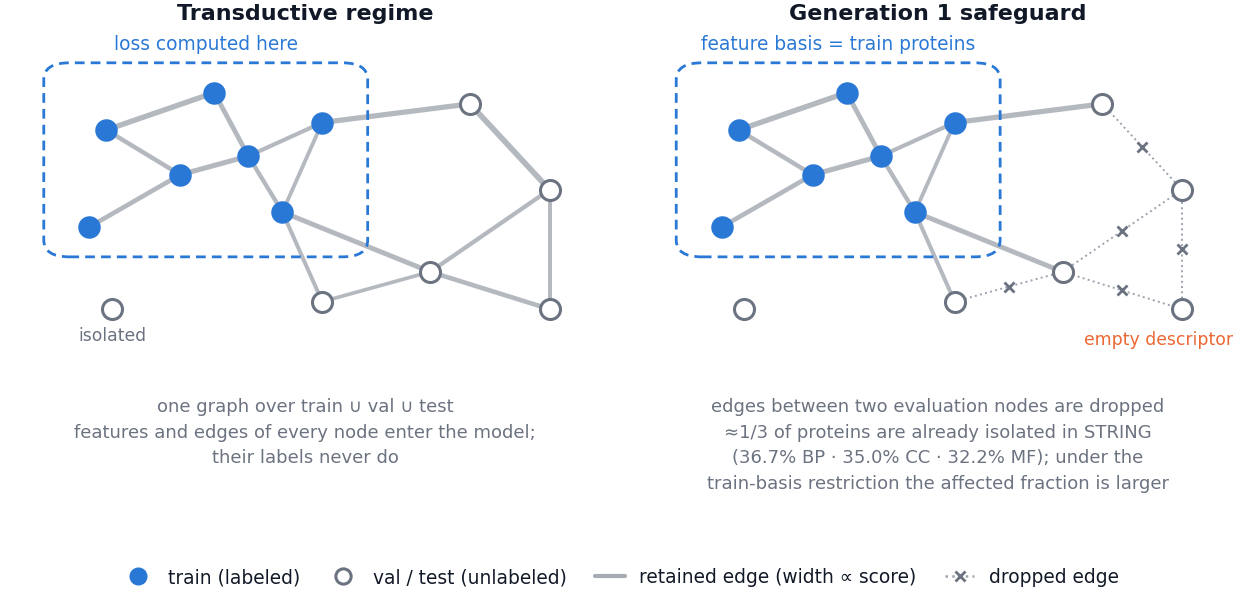
\includegraphics[width=775.3\px,height=373.3\px]{figures/fig_5_2.png}};
\node[tl] at (88,70) {\fmR\fz{16}{16}\color{inkii}\ls{2}\Ll{3 · Data and evaluation}};
\node[tl] at (88,131) {\fdA\fz{54}{56.7}\color{ink}\ls{-1}\Ll{Learning regime and protocol}};
\node<2-4>[tl] at (88,646.3) {\fmR\fz{15}{19.5}\color{muted}\Ll{Dissertation, Fig. 5.2}};
\node<2-4>[tl] at (973.3,232) {\fbR\fz{26}{35.1}\color{ink}\Ll{One graph over train $\cup$ validation $\cup$ test; labels\\read only for training proteins}};
\node<3-4>[tl] at (973.3,318.2) {\fbR\fz{26}{35.1}\color{ink}\Ll{Every design decision on validation; test\\read once}};
\node<4>[tl] at (973.3,404.4) {\fbR\fz{26}{35.1}\color{ink}\Ll{Single seed: differences below 0.5 pp are ties\\(interpretability floor)}};
\node[tr] at (1512,876) {\fmR\fz{16}{16}\color{muted}17 / 45};
\end{tikzpicture}
\note{Validation and test proteins contribute features and edges but never labels. The first generation uses a stricter train-basis construction. 

With a single seed, the talk treats sub-0.5 pp gaps as ties.}
\end{frame}

\section{4 · Method}
\begin{frame}[plain]
\begin{tikzpicture}[deck]
\node<1>[box] at (0,0) {\includegraphics[page=3,width=1600\px]{build/layers}};
\node<2>[box] at (0,0) {\includegraphics[page=50,width=1600\px]{build/layers}};
\node<3-4>[box] at (0,0) {\includegraphics[page=51,width=1600\px]{build/layers}};
\node<5>[box] at (0,0) {\includegraphics[page=52,width=1600\px]{build/layers}};
\node<2-5>[box] at (109,235) {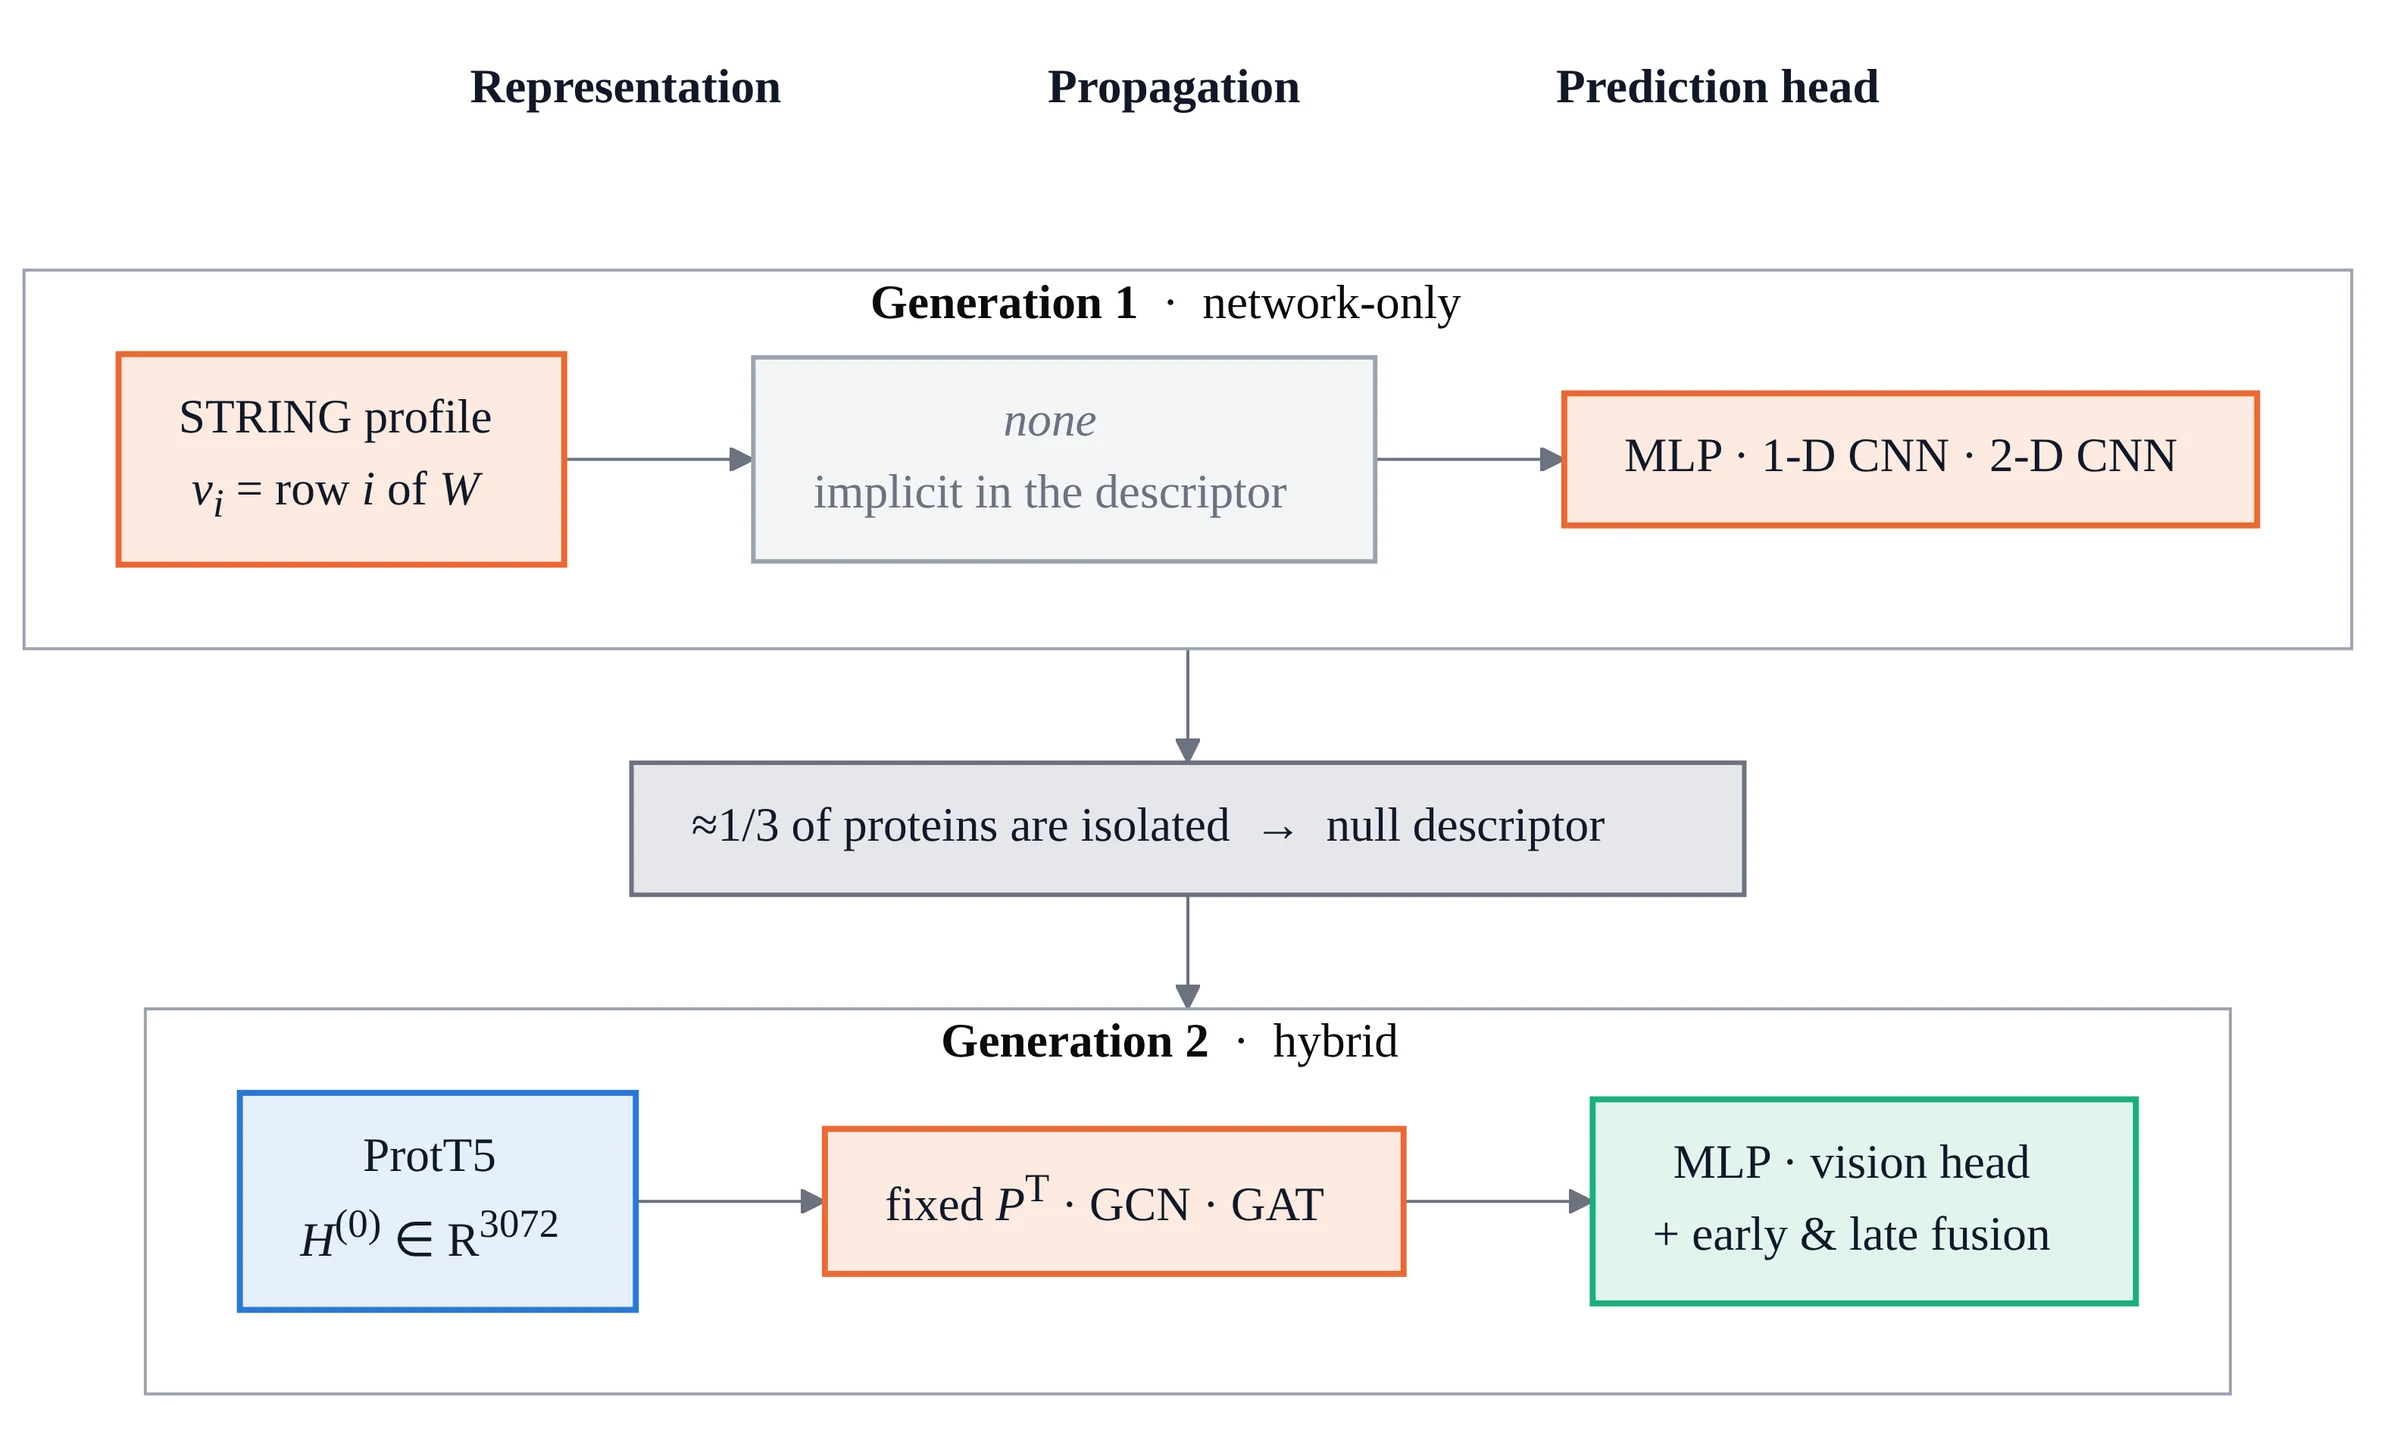
\includegraphics[width=896.7\px,height=535.4\px]{figures/fig_5_1.png}};
\fill<2>[plate] (109,315.3) rectangle ++(896.7,182);
\fill<2-3>[plate] (109,497.3) rectangle ++(896.7,91);
\fill<2-4>[plate] (109,588.3) rectangle ++(896.7,182);
\node[tl] at (88,70) {\fmR\fz{16}{16}\color{inkii}\ls{2}\Ll{4 · Method}};
\node[tl] at (88,131) {\fdA\fz{54}{56.7}\color{ink}\ls{-1}\Ll{Two generations, three decisions}};
\node<2-5>[tl] at (88,808.4) {\fmR\fz{15}{19.5}\color{muted}\Ll{Dissertation, Fig. 5.1}};
\node<2-5>[tl] at (1094.7,236) {\fbR\fz{30}{40.5}\color{ink}\Ll{Representation $\rightarrow$ Propagation\\$\rightarrow$ Prediction head}};
\node<3-5>[tl] at (1094.7,339) {\fbR\fz{30}{40.5}\color{ink}\Ll{Generation 1: network only}};
\node<5>[tl] at (1094.7,401.5) {\fbR\fz{30}{40.5}\color{ink}\Ll{Generation 2 (NEXUS-GO):\\ProtT5 + network}};
\node[tr] at (1512,876) {\fmR\fz{16}{16}\color{muted}18 / 45};
\end{tikzpicture}
\note{Every model decomposes into the same three decisions: representation, propagation and prediction head. 

The limitation of the first generation is a property of its input, about one third of the proteins get a null descriptor, and it motivates the second.}
\end{frame}

\begin{frame}[plain]
\begin{tikzpicture}[deck]
\node<1>[box] at (0,0) {\includegraphics[page=3,width=1600\px]{build/layers}};
\node<2>[box] at (0,0) {\includegraphics[page=53,width=1600\px]{build/layers}};
\node<3>[box] at (0,0) {\includegraphics[page=54,width=1600\px]{build/layers}};
\node<4>[box] at (0,0) {\includegraphics[page=55,width=1600\px]{build/layers}};
\node<2-4>[box] at (109,235) {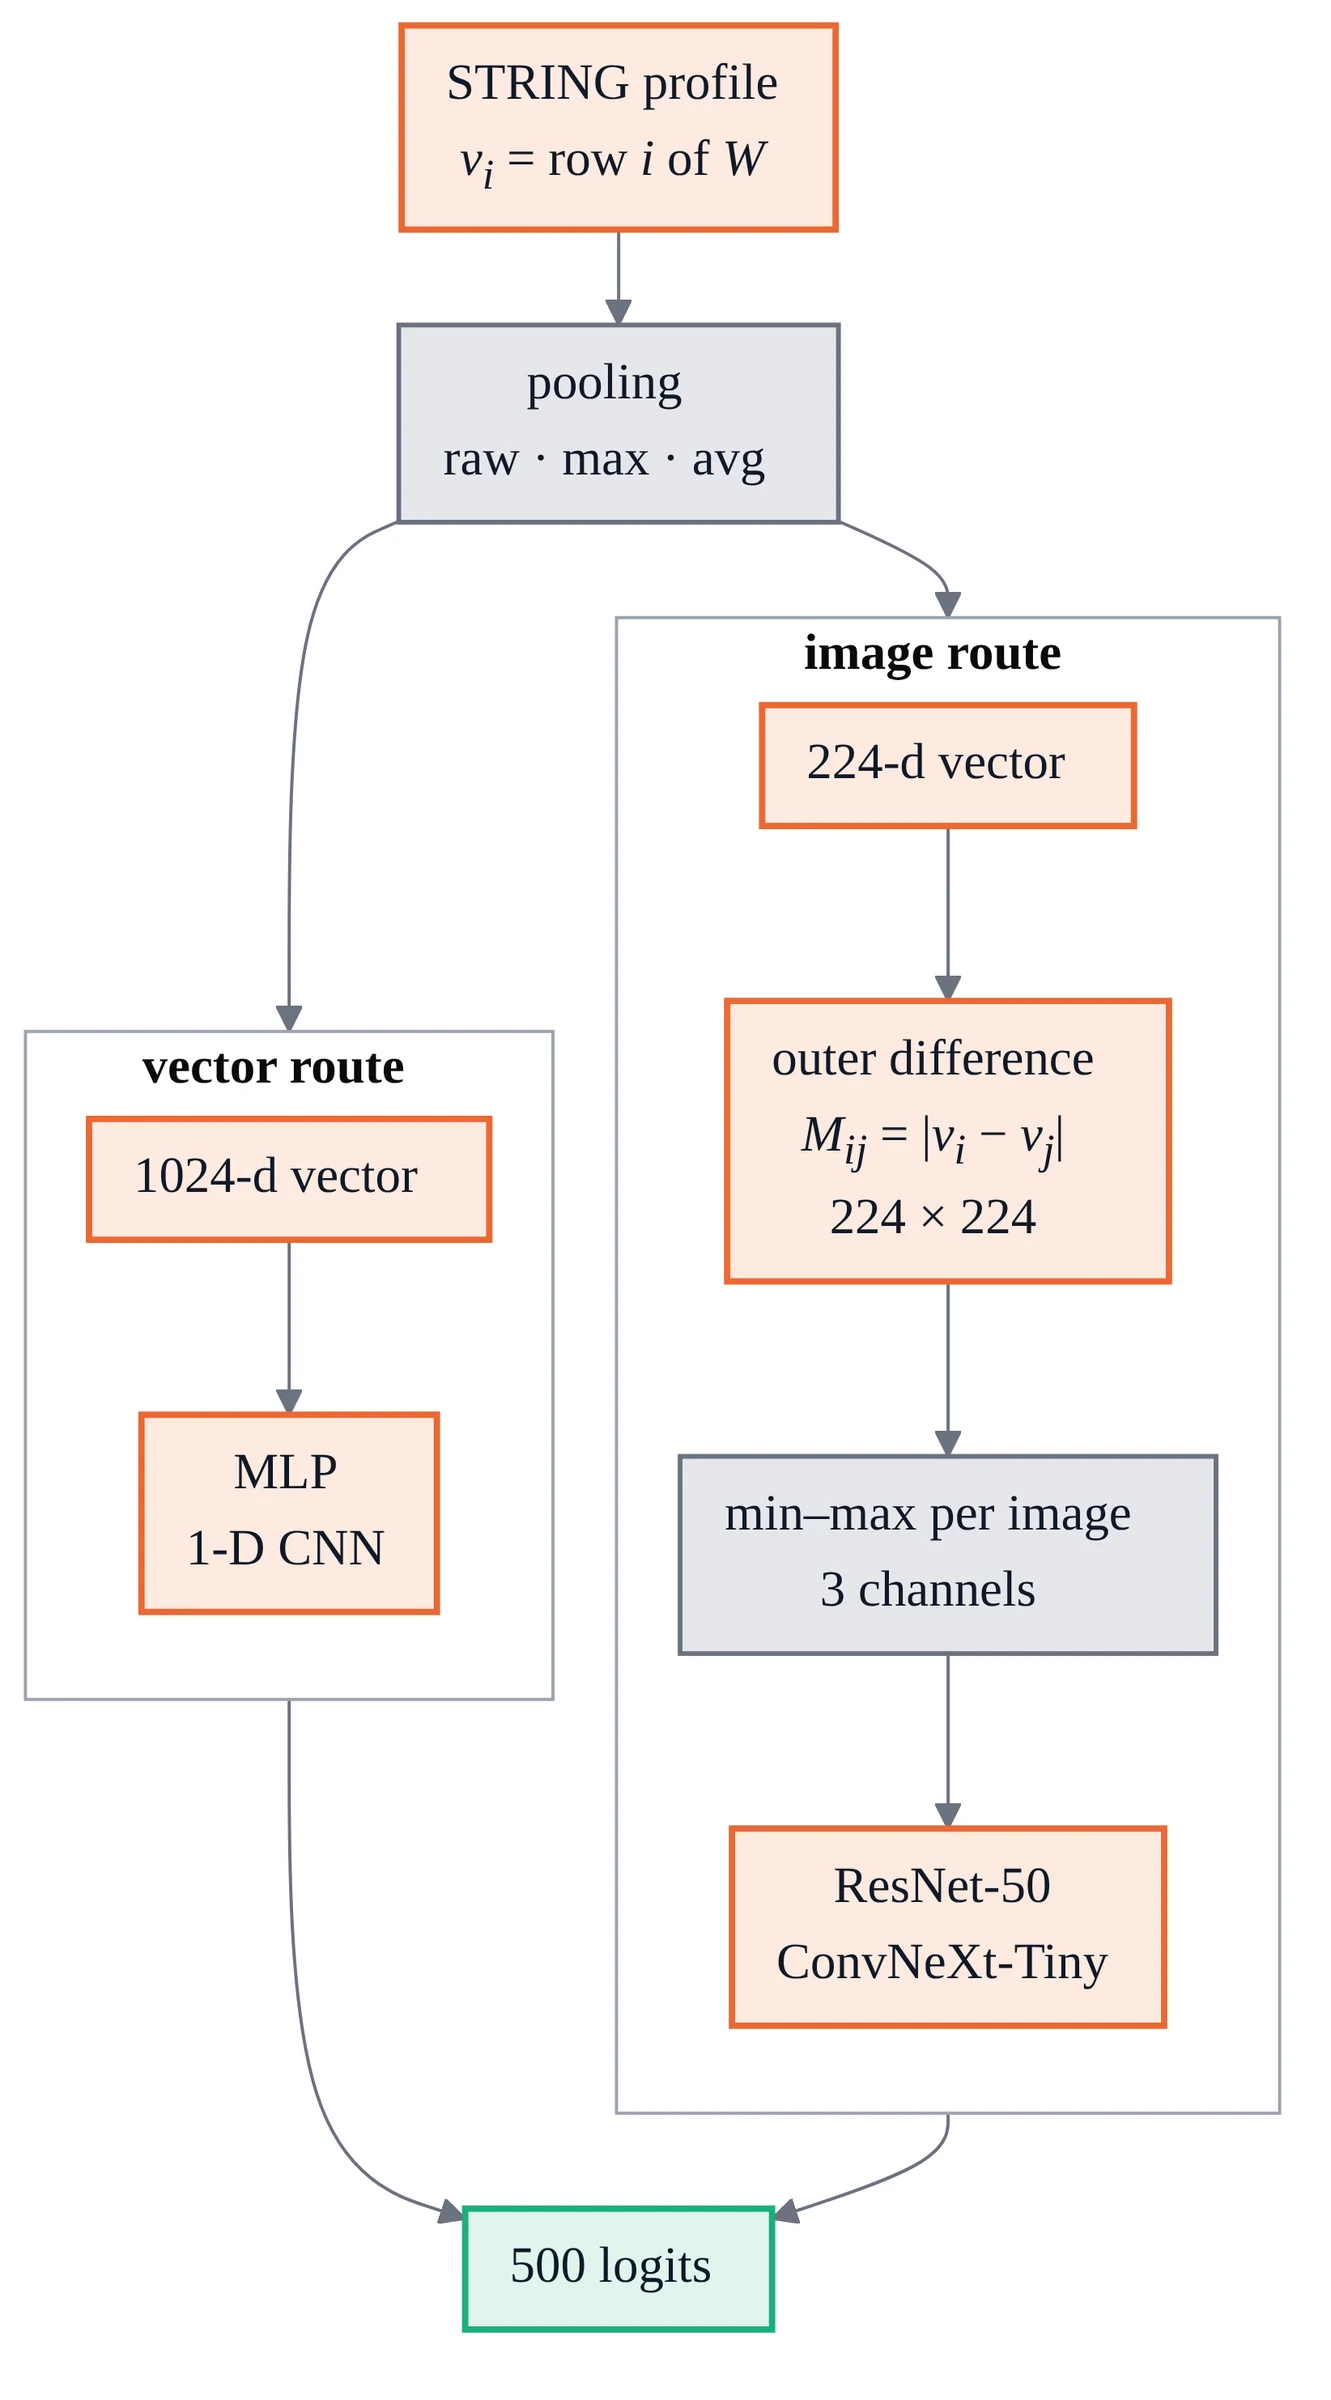
\includegraphics[width=299.5\px,height=540\px]{figures/fig_5_3.png}};
\node<4>[box] at (473,512.5) {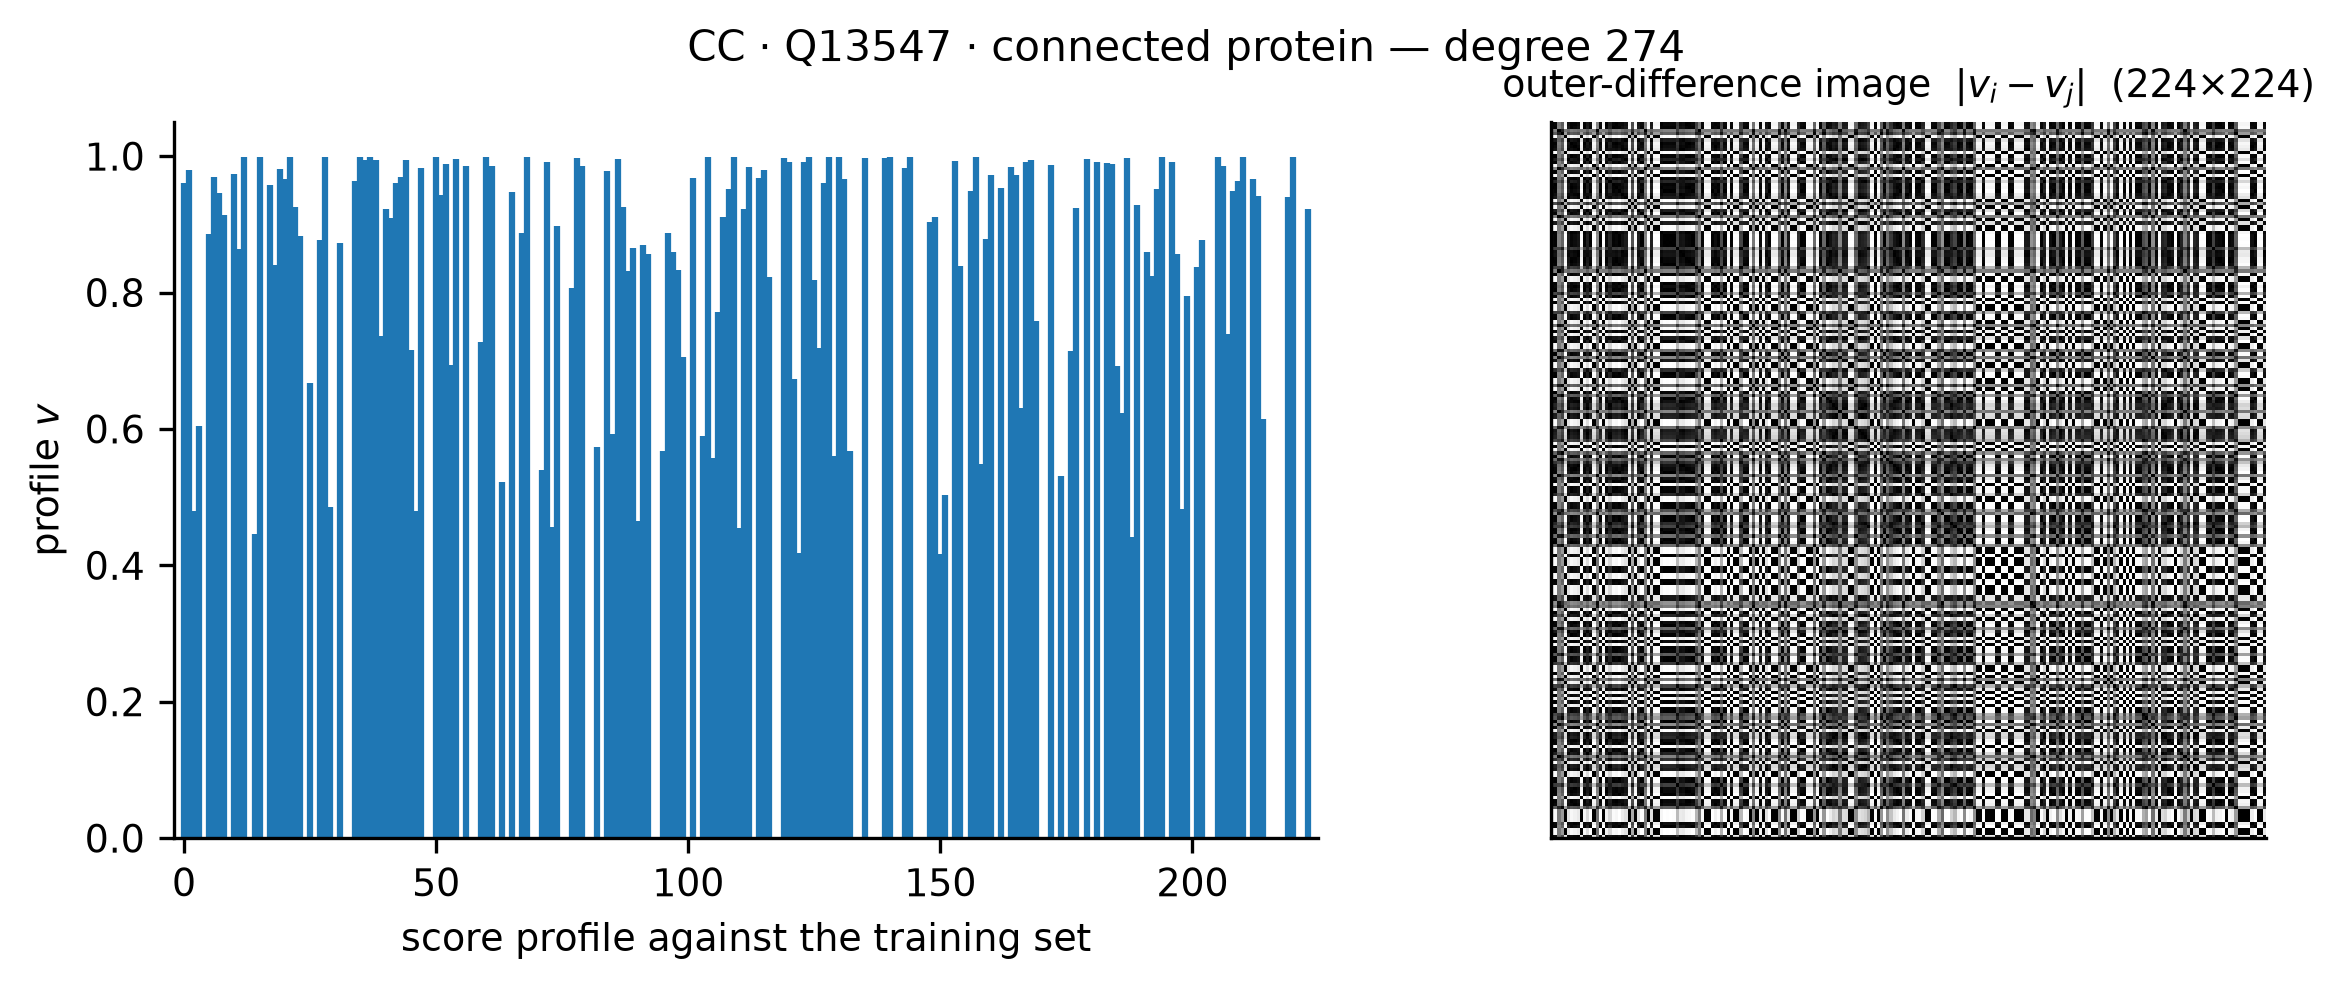
\includegraphics[width=592.2\px,height=250\px]{figures/fig_5_4.png}};
\node[tl] at (88,70) {\fmR\fz{16}{16}\color{inkii}\ls{2}\Ll{4 · Method}};
\node[tl] at (88,131) {\fdA\fz{54}{56.7}\color{ink}\ls{-1}\Ll{Generation 1: the network alone}};
\node<2-4>[tl] at (88,813) {\fmR\fz{15}{19.5}\color{muted}\Ll{Dissertation, Fig. 5.3}};
\node<2-4>[tl] at (488,232) {\fbR\fz{26}{35.1}\color{ink}\Ll{Input: row of the weighted adjacency, against training proteins}};
\node<2-4>[tl] at (488,283.1) {\fbR\fz{26}{35.1}\color{ink}\Ll{Pooling: raw, max, avg}};
\node<3-4>[tl] at (488,334.2) {\fbR\fz{26}{35.1}\color{ink}\Ll{Vector route: MLP or 1-D CNN}};
\node<4>[tl] at (488,385.3) {\fbR\fz{26}{35.1}\color{ink}\Ll{Image route: outer-difference matrix {\fz{29.2}{35}$|v_i - v_j|$}, 224 × 224, ResNet-50 or ConvNeXt-Tiny}};
\node<4>[tl] at (488,436.4) {\fbR\fz{26}{35.1}\color{ink}\Ll{Floor: a naive guilt-by-association baseline}};
\node<4>[tl] at (452,800.5) {\fmR\fz{15}{19.5}\color{muted}\Ll{Dissertation, Fig. 5.4}};
\node[tr] at (1512,876) {\fmR\fz{16}{16}\color{muted}19 / 45};
\end{tikzpicture}
\note{The descriptor is already a one-hop aggregation, so there is no separate propagation stage. 

The image route imports a convolutional bias into a non-visual vector, as SUPERMAGOv2 and DeepInsight did with isolated descriptors.}
\end{frame}

\begin{frame}[plain]
\begin{tikzpicture}[deck]
\node<1>[box] at (0,0) {\includegraphics[page=3,width=1600\px]{build/layers}};
\node<2>[box] at (0,0) {\includegraphics[page=56,width=1600\px]{build/layers}};
\node<3>[box] at (0,0) {\includegraphics[page=57,width=1600\px]{build/layers}};
\node<4>[box] at (0,0) {\includegraphics[page=58,width=1600\px]{build/layers}};
\node<2-4>[box] at (109,235) {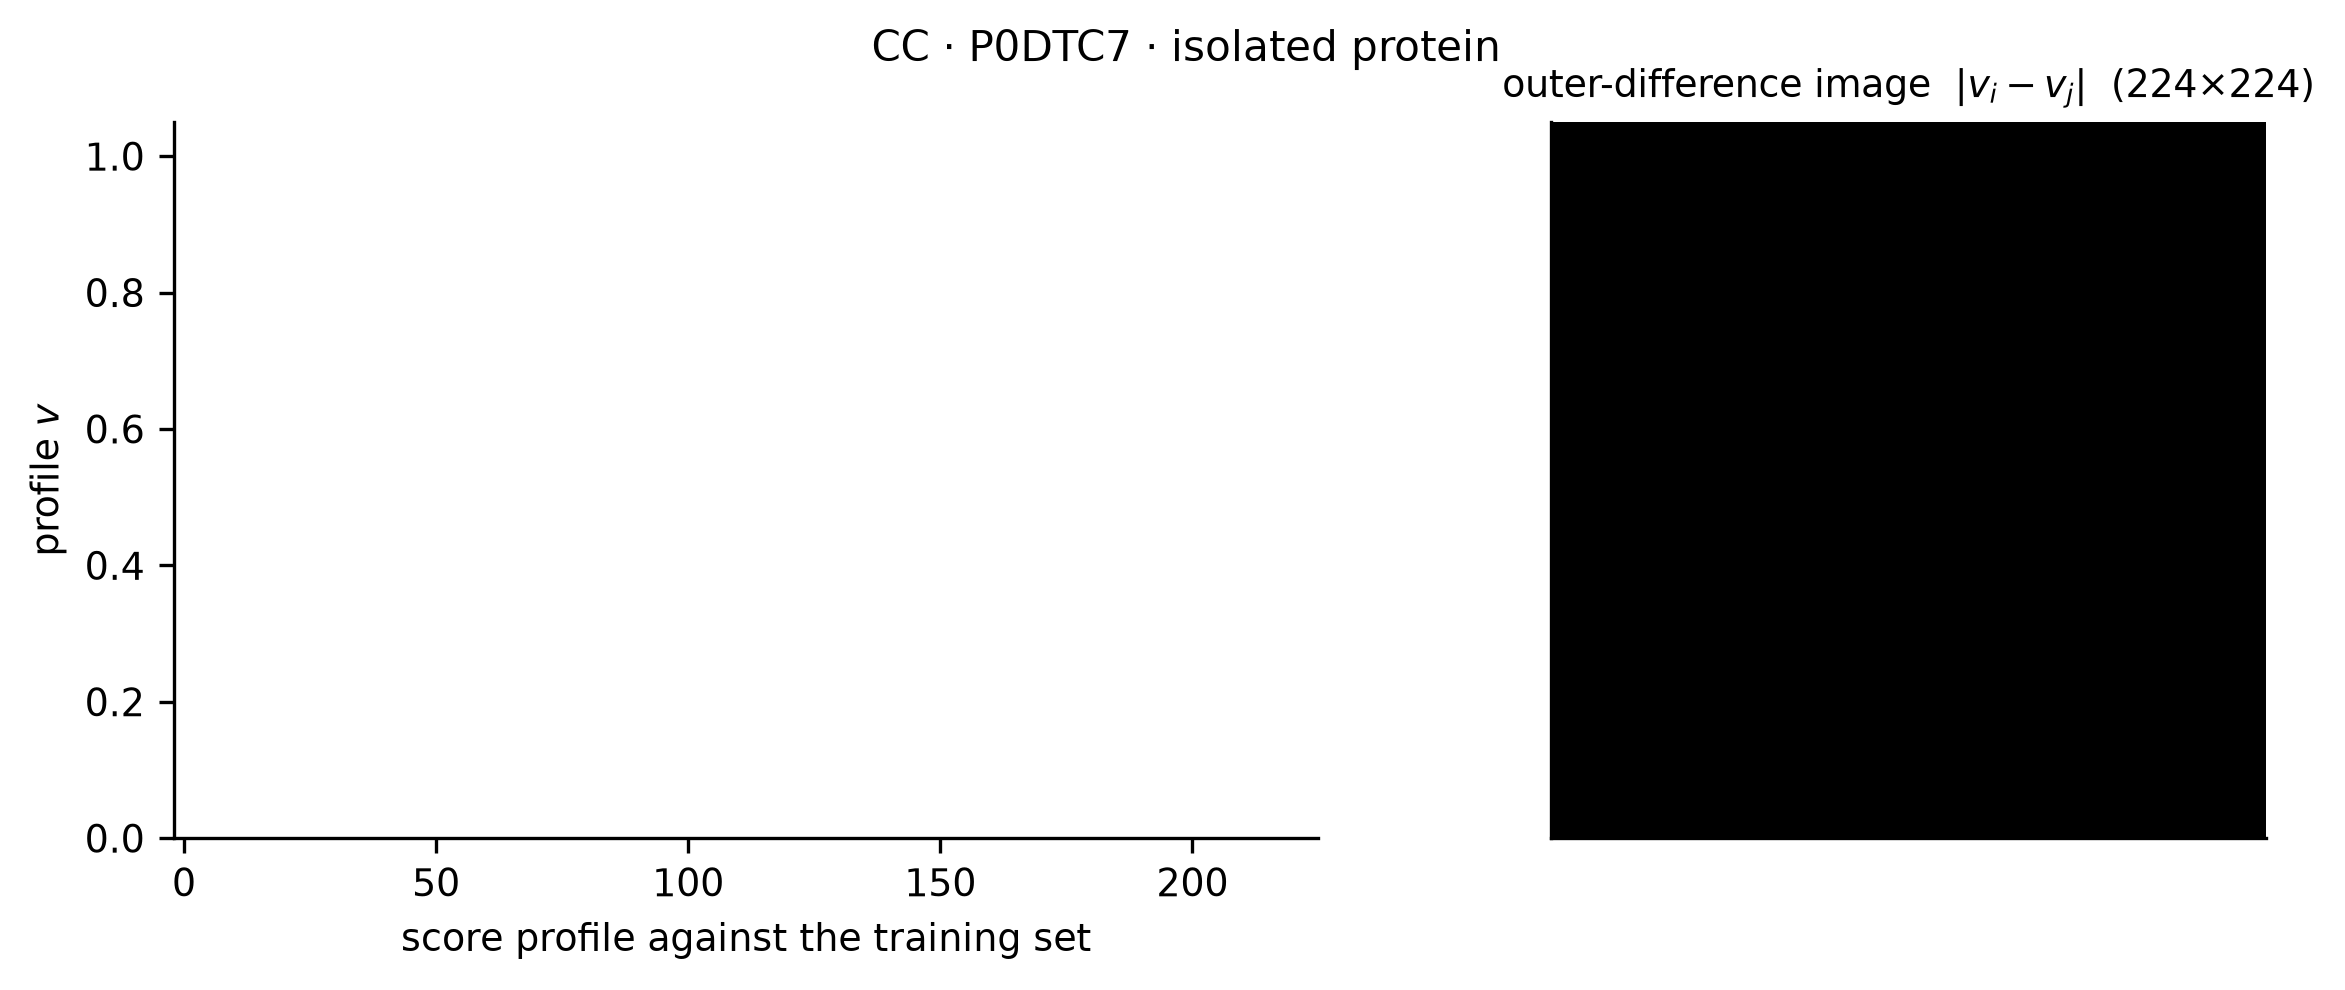
\includegraphics[width=654\px,height=276.1\px]{figures/fig_5_5.png}};
\node<2-4>[box] at (837,235) {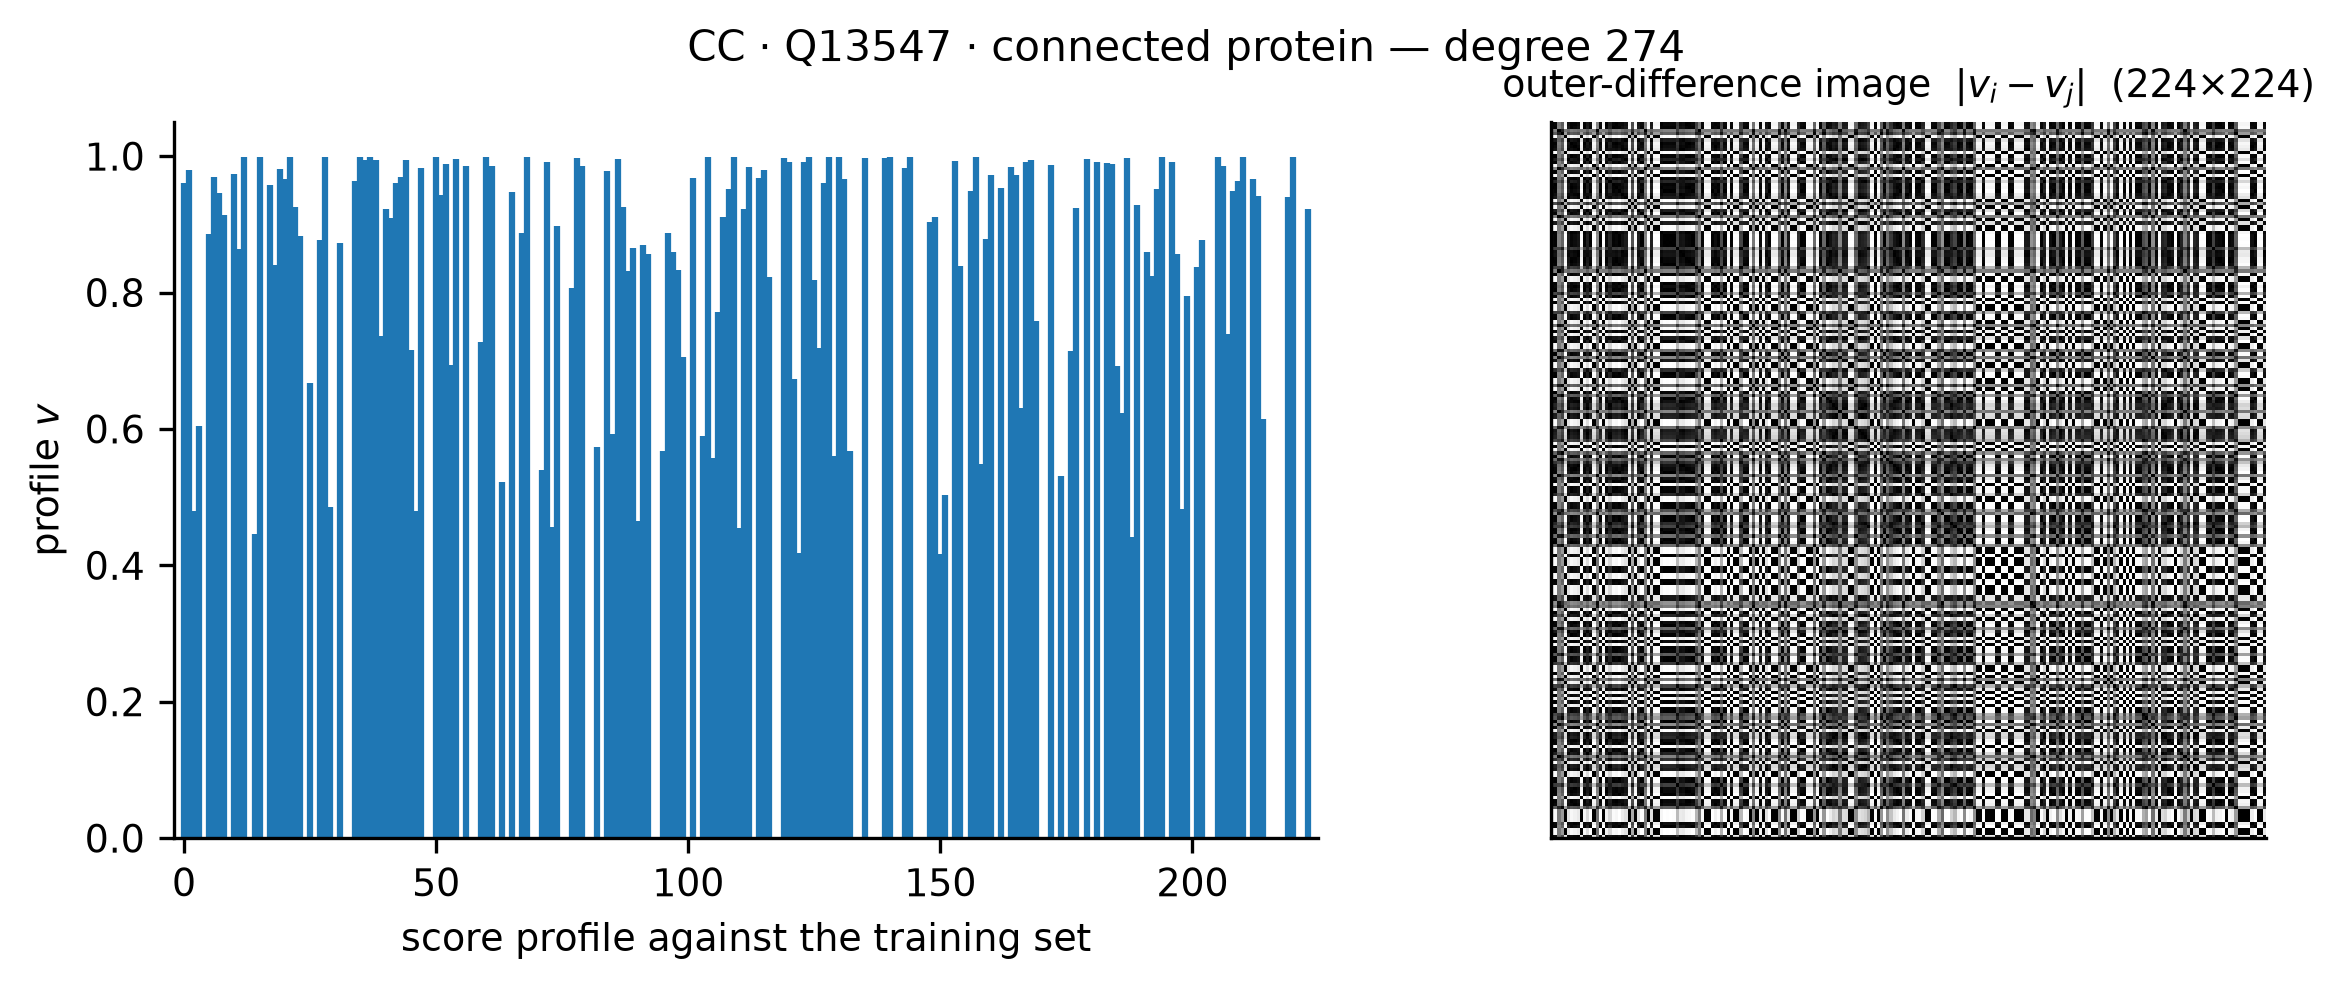
\includegraphics[width=654\px,height=276.1\px]{figures/fig_5_4.png}};
\node[tl] at (88,70) {\fmR\fz{16}{16}\color{inkii}\ls{2}\Ll{4 · Method}};
\node[tl] at (88,131) {\fdA\fz{54}{56.7}\color{ink}\ls{-1}\Ll{An isolated protein has no input}};
\node<2-4>[tl] at (88,549.1) {\fmR\fz{15}{19.5}\color{muted}\Ll{Dissertation, Fig. 5.5 · isolated vs connected}};
\node<2-4>[tl] at (816,549.1) {\fmR\fz{15}{19.5}\color{muted}\Ll{Dissertation, Fig. 5.4 · for contrast}};
\node<3-4>[tl] at (124,583.3) {\fbR\fz{30}{40.5}\color{ink}\Ll{Null profile $\rightarrow$ null matrix $\rightarrow$ uniform image}};
\node<3-4>[tl] at (124,645.8) {\fbR\fz{30}{40.5}\color{ink}\Ll{The head can only return the class prior}};
\node<3-4>[tl] at (124,708.3) {\fbR\fz{30}{40.5}\color{ink}\Ll{No architecture can recover what is absent}};
\node<4>[tl] at (846,779.8) {\fdA\fz{38}{45.6}\color{ink}\Ll{Requirement: a representation\\that exists for every protein}};
\node[tr] at (1512,876) {\fmR\fz{16}{16}\color{muted}20 / 45};
\end{tikzpicture}
\note{For a third of the corpus the first generation sees nothing. 

The amino-acid sequence satisfies the requirement by construction, and that is where the second generation starts.}
\end{frame}

\begin{frame}[plain]
\hypertarget<1>{s21.1}{}
\hypertarget<2>{s21.2}{}
\hypertarget<3>{s21.3}{}
\hypertarget<4>{s21.4}{}
\hypertarget<5>{s21.5}{}
\hypertarget<6>{s21.6}{}
\hypertarget<7>{s21.7}{}
\hypertarget<8>{s21.8}{}
\begin{tikzpicture}[deck]
\node<1>[box] at (0,0) {\includegraphics[page=59,width=1600\px]{build/layers}};
\node<2>[box] at (0,0) {\includegraphics[page=60,width=1600\px]{build/layers}};
\node<3>[box] at (0,0) {\includegraphics[page=61,width=1600\px]{build/layers}};
\node<4>[box] at (0,0) {\includegraphics[page=62,width=1600\px]{build/layers}};
\node<5>[box] at (0,0) {\includegraphics[page=63,width=1600\px]{build/layers}};
\node<6>[box] at (0,0) {\includegraphics[page=64,width=1600\px]{build/layers}};
\node<7>[box] at (0,0) {\includegraphics[page=65,width=1600\px]{build/layers}};
\node<8>[box] at (0,0) {\includegraphics[page=66,width=1600\px]{build/layers}};
\node<4-8>[box] at (207.4,206) {\hot{89.1}{42}{s21.4}};
\node<4-8>[box] at (295,206) {\hot{82.5}{42}{s21.5}};
\node<4-8>[box] at (376,206) {\hot{84.8}{42}{s21.6}};
\node<4-8>[box] at (459.4,206) {\hot{80}{42}{s21.7}};
\node<4-8>[box] at (152,206) {\hot{56.9}{42}{s21.8}};
\node<4-8>[box] at (1315.5,206) {\hot{196.5}{42}{s21fig}};
\fill<8>[slide] (86,204) rectangle ++(1428,544); \node<8>[box] at (88,206) {\animategraphics[autoplay,loop,width=1424\px]{10}{build/seq/pipe-anim}{}{}};
\node[tl] at (88,70) {\fmR\fz{16}{16}\color{inkii}\ls{2}\Ll{4 · Method}};
\node[tl] at (88,131) {\fdA\fz{54}{56.7}\color{ink}\ls{-1}\Ll{NEXUS-GO: four routes}};
\node<2-8>[tl] at (88,803.1) {\fbR\fz{24}{31.2}\color{ink}\Ll{Sequence $\rightarrow$ ProtT5 $\rightarrow$ {\fz{26.9}{32.3}$\mathbf{H}^{(0)} \in \mathbb{R}^{3072}$}}};
\node<3-8>[tl] at (573.3,802) {\fbR\fz{24}{31.2}\color{ink}\Ll{STRING $\rightarrow$ weighted graph {\fz{26.9}{32.3}$W$} $\rightarrow$\\{\fz{26.9}{32.3}$P = W D_c^{-1}$}}};
\node<4-8>[tl] at (1058.7,802) {\fbR\fz{24}{31.2}\color{ink}\Ll{Routes: /Fixed · /GNN · /Early · /Late}};
\node[tr] at (1512,876) {\fmR\fz{16}{16}\color{muted}21 / 45};
\end{tikzpicture}
\note{Two inputs, two propagation routes and two ways of combining them. 

The first generation is reported as a topology-only control and carries no route name.}
\end{frame}

\begin{frame}[plain]
\begin{tikzpicture}[deck]
\node<1>[box] at (0,0) {\includegraphics[page=3,width=1600\px]{build/layers}};
\node<2>[box] at (0,0) {\includegraphics[page=67,width=1600\px]{build/layers}};
\node<3>[box] at (0,0) {\includegraphics[page=68,width=1600\px]{build/layers}};
\node<4>[box] at (0,0) {\includegraphics[page=69,width=1600\px]{build/layers}};
\node<2-4>[box] at (109,235) {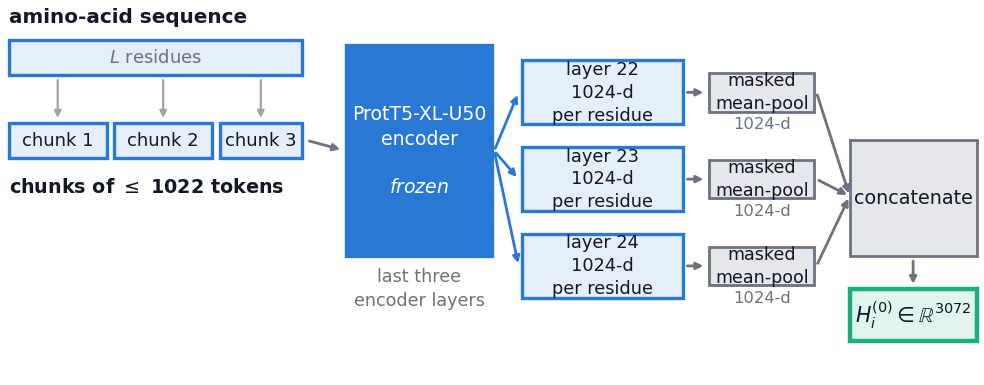
\includegraphics[width=1022.3\px,height=400\px]{figures/fig_5_7.png}};
\node[tl] at (88,70) {\fmR\fz{16}{16}\color{inkii}\ls{2}\Ll{4 · Method}};
\node[tl] at (88,131) {\fdA\fz{54}{56.7}\color{ink}\ls{-1}\Ll{ProtT5-XL-U50, three layers, frozen}};
\node<2-4>[tl] at (88,673) {\fmR\fz{15}{19.5}\color{muted}\Ll{Dissertation, Fig. 5.7}};
\node<2-4>[tl] at (124,729.5) {\fbR\fz{26}{35.1}\color{ink}\Ll{Chunks of at most 1,022 residues;\\masked mean-pool, then mean\\over chunks}};
\node<3-4>[tl] at (609.3,729.5) {\fbR\fz{26}{35.1}\color{ink}\Ll{Layers 24, 23, 22, concatenated: 3 ×\\1024 = 3072 dimensions}};
\node<4>[tl] at (1094.7,729.5) {\fbR\fz{26}{35.1}\color{ink}\Ll{Exists for every protein, isolated\\or not}};
\node[tr] at (1512,876) {\fmR\fz{16}{16}\color{muted}22 / 45};
\end{tikzpicture}
\note{Reading three adjacent layers avoids committing to one point between the pretraining objective and structural signal, at no tuning cost. 

Extraction is inherited from SUPERMAGOv2.}
\end{frame}

\begin{frame}[plain]
\hypertarget<1>{s23.1}{}
\hypertarget<2>{s23.2}{}
\hypertarget<3>{s23.3}{}
\hypertarget<4>{s23.4}{}
\hypertarget<5>{s23.5}{}
\begin{tikzpicture}[deck]
\node<1>[box] at (0,0) {\includegraphics[page=3,width=1600\px]{build/layers}};
\node<2>[box] at (0,0) {\includegraphics[page=70,width=1600\px]{build/layers}};
\node<3>[box] at (0,0) {\includegraphics[page=71,width=1600\px]{build/layers}};
\node<4>[box] at (0,0) {\includegraphics[page=72,width=1600\px]{build/layers}};
\node<5>[box] at (0,0) {\includegraphics[page=73,width=1600\px]{build/layers}};
\node<3-5>[box] at (749.1,206) {\hot{71.1}{42}{s23.4}};
\node<3-5>[box] at (818.7,206) {\hot{71}{42}{s23.5}};
\node[tl] at (88,70) {\fmR\fz{16}{16}\color{inkii}\ls{2}\Ll{4 · Method}};
\node[tl] at (88,131) {\fdA\fz{54}{56.7}\color{ink}\ls{-1}\Ll{From records to an operator}};
\node<2-5>[tl] at (124,236) {\fbR\fz{30}{40.5}\color{ink}\Ll{Symmetric, no self-loops, sparse COO: at\\most 1,133,132 stored entries (dense: 25\\to 35 GB)}};
\node<3-5>[tl] at (124,379.5) {\fbR\fz{30}{40.5}\color{ink}\Ll{Deduplication: max keeps the score;\\sum multiplies it by the record count}};
\node<4-5>[tl] at (124,482.5) {\fbR\fz{30}{40.5}\color{ink}\Ll{Column-stochastic {\fz{33.7}{40.4}$P = W D_c^{-1}$}: weights\\are relative to each protein's neighbours}};
\node[tr] at (1512,876) {\fmR\fz{16}{16}\color{muted}23 / 45};
\end{tikzpicture}
\note{Repeated records carry no extra score, so summing rewards how often a pair was written down. The maximum keeps the STRING score on its own scale. 

Normalization does not undo the reordering.}
\end{frame}

\begin{frame}[plain]
\hypertarget<1>{s24.1}{}
\hypertarget<2>{s24.2}{}
\hypertarget<3>{s24.3}{}
\hypertarget<4>{s24.4}{}
\hypertarget<5>{s24.5}{}
\hypertarget<6>{s24.6}{}
\hypertarget<7>{s24.7}{}
\hypertarget<8>{s24.8}{}
\begin{tikzpicture}[deck]
\node<1-2>[box] at (0,0) {\includegraphics[page=3,width=1600\px]{build/layers}};
\node<3>[box] at (0,0) {\includegraphics[page=74,width=1600\px]{build/layers}};
\node<4>[box] at (0,0) {\includegraphics[page=75,width=1600\px]{build/layers}};
\node<5,8>[box] at (0,0) {\includegraphics[page=76,width=1600\px]{build/layers}};
\node<6>[box] at (0,0) {\includegraphics[page=77,width=1600\px]{build/layers}};
\node<7>[box] at (0,0) {\includegraphics[page=78,width=1600\px]{build/layers}};
\node<3>[box] at (800.2,211) {\hot{13.6}{32}{s24.6}};
\node<3>[box] at (813.9,211) {\hot{11.2}{32}{s24x.46}};
\node<3>[box] at (825,211) {\hot{11.2}{32}{s24.5}};
\node<3>[box] at (836.2,211) {\hot{11.2}{32}{s24x.48}};
\node<3>[box] at (847.5,211) {\hot{11.2}{32}{s24x.49}};
\node<3>[box] at (858.6,211) {\hot{11.2}{32}{s24x.50}};
\node<3>[box] at (869.9,211) {\hot{11.2}{32}{s24.7}};
\node<3>[box] at (881,211) {\hot{11.2}{32}{s24x.52}};
\node<3>[box] at (892.2,211) {\hot{11.2}{32}{s24x.53}};
\node<3>[box] at (903.5,211) {\hot{11.2}{32}{s24x.54}};
\node<3>[box] at (914.6,211) {\hot{13.6}{32}{s24x.55}};
\node<3>[box] at (1139.7,211) {\hot{15}{32}{s24x.3}};
\node<3>[box] at (1154.7,211) {\hot{14}{32}{s24x.14}};
\node<3>[box] at (1168.7,211) {\hot{14}{32}{s24x.25}};
\node<3>[box] at (1182.7,211) {\hot{14}{32}{s24x.36}};
\node<3>[box] at (1196.7,211) {\hot{14}{32}{s24.5}};
\node<3>[box] at (1210.7,211) {\hot{14}{32}{s24x.58}};
\node<3>[box] at (1224.7,211) {\hot{14}{32}{s24x.69}};
\node<3>[box] at (1238.7,211) {\hot{14}{32}{s24x.80}};
\node<3>[box] at (1252.7,211) {\hot{15}{32}{s24x.91}};
\node<3>[box] at (1337.3,206) {\hot{70.2}{42}{s24.8}};
\node<4>[box] at (800.2,211) {\hot{13.6}{32}{s24.6}};
\node<4>[box] at (813.9,211) {\hot{11.2}{32}{s24x.46}};
\node<4>[box] at (825,211) {\hot{11.2}{32}{s24.5}};
\node<4>[box] at (836.2,211) {\hot{11.2}{32}{s24x.48}};
\node<4>[box] at (847.5,211) {\hot{11.2}{32}{s24x.49}};
\node<4>[box] at (858.6,211) {\hot{11.2}{32}{s24x.50}};
\node<4>[box] at (869.9,211) {\hot{11.2}{32}{s24.7}};
\node<4>[box] at (881,211) {\hot{11.2}{32}{s24x.52}};
\node<4>[box] at (892.2,211) {\hot{11.2}{32}{s24x.53}};
\node<4>[box] at (903.5,211) {\hot{11.2}{32}{s24x.54}};
\node<4>[box] at (914.6,211) {\hot{13.6}{32}{s24x.55}};
\node<4>[box] at (1139.7,211) {\hot{15}{32}{s24x.3}};
\node<4>[box] at (1154.7,211) {\hot{14}{32}{s24x.14}};
\node<4>[box] at (1168.7,211) {\hot{14}{32}{s24x.25}};
\node<4>[box] at (1182.7,211) {\hot{14}{32}{s24x.36}};
\node<4>[box] at (1196.7,211) {\hot{14}{32}{s24.5}};
\node<4>[box] at (1210.7,211) {\hot{14}{32}{s24x.58}};
\node<4>[box] at (1224.7,211) {\hot{14}{32}{s24x.69}};
\node<4>[box] at (1238.7,211) {\hot{14}{32}{s24x.80}};
\node<4>[box] at (1252.7,211) {\hot{15}{32}{s24x.91}};
\node<4>[box] at (1337.3,206) {\hot{70.2}{42}{s24.8}};
\node<5>[box] at (800.2,211) {\hot{13.6}{32}{s24.6}};
\node<5>[box] at (813.9,211) {\hot{11.2}{32}{s24x.46}};
\node<5>[box] at (825,211) {\hot{11.2}{32}{s24.5}};
\node<5>[box] at (836.2,211) {\hot{11.2}{32}{s24x.48}};
\node<5>[box] at (847.5,211) {\hot{11.2}{32}{s24x.49}};
\node<5>[box] at (858.6,211) {\hot{11.2}{32}{s24x.50}};
\node<5>[box] at (869.9,211) {\hot{11.2}{32}{s24.7}};
\node<5>[box] at (881,211) {\hot{11.2}{32}{s24x.52}};
\node<5>[box] at (892.2,211) {\hot{11.2}{32}{s24x.53}};
\node<5>[box] at (903.5,211) {\hot{11.2}{32}{s24x.54}};
\node<5>[box] at (914.6,211) {\hot{13.6}{32}{s24x.55}};
\node<5>[box] at (1139.7,211) {\hot{15}{32}{s24x.3}};
\node<5>[box] at (1154.7,211) {\hot{14}{32}{s24x.14}};
\node<5>[box] at (1168.7,211) {\hot{14}{32}{s24x.25}};
\node<5>[box] at (1182.7,211) {\hot{14}{32}{s24x.36}};
\node<5>[box] at (1196.7,211) {\hot{14}{32}{s24.5}};
\node<5>[box] at (1210.7,211) {\hot{14}{32}{s24x.58}};
\node<5>[box] at (1224.7,211) {\hot{14}{32}{s24x.69}};
\node<5>[box] at (1238.7,211) {\hot{14}{32}{s24x.80}};
\node<5>[box] at (1252.7,211) {\hot{15}{32}{s24x.91}};
\node<5>[box] at (1337.3,206) {\hot{70.2}{42}{s24.8}};
\node<6>[box] at (800.2,211) {\hot{13.6}{32}{s24.6}};
\node<6>[box] at (813.9,211) {\hot{11.2}{32}{s24x.46}};
\node<6>[box] at (825,211) {\hot{11.2}{32}{s24.5}};
\node<6>[box] at (836.2,211) {\hot{11.2}{32}{s24x.48}};
\node<6>[box] at (847.5,211) {\hot{11.2}{32}{s24x.49}};
\node<6>[box] at (858.6,211) {\hot{11.2}{32}{s24x.50}};
\node<6>[box] at (869.9,211) {\hot{11.2}{32}{s24.7}};
\node<6>[box] at (881,211) {\hot{11.2}{32}{s24x.52}};
\node<6>[box] at (892.2,211) {\hot{11.2}{32}{s24x.53}};
\node<6>[box] at (903.5,211) {\hot{11.2}{32}{s24x.54}};
\node<6>[box] at (914.6,211) {\hot{13.6}{32}{s24x.55}};
\node<6>[box] at (1139.7,211) {\hot{15}{32}{s24x.1}};
\node<6>[box] at (1154.7,211) {\hot{14}{32}{s24x.12}};
\node<6>[box] at (1168.7,211) {\hot{14}{32}{s24x.23}};
\node<6>[box] at (1182.7,211) {\hot{14}{32}{s24x.34}};
\node<6>[box] at (1196.7,211) {\hot{14}{32}{s24.6}};
\node<6>[box] at (1210.7,211) {\hot{14}{32}{s24x.56}};
\node<6>[box] at (1224.7,211) {\hot{14}{32}{s24x.67}};
\node<6>[box] at (1238.7,211) {\hot{14}{32}{s24x.78}};
\node<6>[box] at (1252.7,211) {\hot{15}{32}{s24x.89}};
\node<6>[box] at (1337.3,206) {\hot{70.2}{42}{s24.8}};
\node<7>[box] at (800.2,211) {\hot{13.6}{32}{s24.6}};
\node<7>[box] at (813.9,211) {\hot{11.2}{32}{s24x.46}};
\node<7>[box] at (825,211) {\hot{11.2}{32}{s24.5}};
\node<7>[box] at (836.2,211) {\hot{11.2}{32}{s24x.48}};
\node<7>[box] at (847.5,211) {\hot{11.2}{32}{s24x.49}};
\node<7>[box] at (858.6,211) {\hot{11.2}{32}{s24x.50}};
\node<7>[box] at (869.9,211) {\hot{11.2}{32}{s24.7}};
\node<7>[box] at (881,211) {\hot{11.2}{32}{s24x.52}};
\node<7>[box] at (892.2,211) {\hot{11.2}{32}{s24x.53}};
\node<7>[box] at (903.5,211) {\hot{11.2}{32}{s24x.54}};
\node<7>[box] at (914.6,211) {\hot{13.6}{32}{s24x.55}};
\node<7>[box] at (1139.7,211) {\hot{15}{32}{s24x.7}};
\node<7>[box] at (1154.7,211) {\hot{14}{32}{s24x.18}};
\node<7>[box] at (1168.7,211) {\hot{14}{32}{s24x.29}};
\node<7>[box] at (1182.7,211) {\hot{14}{32}{s24x.40}};
\node<7>[box] at (1196.7,211) {\hot{14}{32}{s24.7}};
\node<7>[box] at (1210.7,211) {\hot{14}{32}{s24x.62}};
\node<7>[box] at (1224.7,211) {\hot{14}{32}{s24x.73}};
\node<7>[box] at (1238.7,211) {\hot{14}{32}{s24x.84}};
\node<7>[box] at (1252.7,211) {\hot{15}{32}{s24x.95}};
\node<7>[box] at (1337.3,206) {\hot{70.2}{42}{s24.8}};
\node<8>[box] at (800.2,211) {\hot{13.6}{32}{s24.6}};
\node<8>[box] at (813.9,211) {\hot{11.2}{32}{s24x.46}};
\node<8>[box] at (825,211) {\hot{11.2}{32}{s24.5}};
\node<8>[box] at (836.2,211) {\hot{11.2}{32}{s24x.48}};
\node<8>[box] at (847.5,211) {\hot{11.2}{32}{s24x.49}};
\node<8>[box] at (858.6,211) {\hot{11.2}{32}{s24x.50}};
\node<8>[box] at (869.9,211) {\hot{11.2}{32}{s24.7}};
\node<8>[box] at (881,211) {\hot{11.2}{32}{s24x.52}};
\node<8>[box] at (892.2,211) {\hot{11.2}{32}{s24x.53}};
\node<8>[box] at (903.5,211) {\hot{11.2}{32}{s24x.54}};
\node<8>[box] at (914.6,211) {\hot{13.6}{32}{s24x.55}};
\node<8>[box] at (1139.7,211) {\hot{15}{32}{s24x.3}};
\node<8>[box] at (1154.7,211) {\hot{14}{32}{s24x.14}};
\node<8>[box] at (1168.7,211) {\hot{14}{32}{s24x.25}};
\node<8>[box] at (1182.7,211) {\hot{14}{32}{s24x.36}};
\node<8>[box] at (1196.7,211) {\hot{14}{32}{s24.5}};
\node<8>[box] at (1210.7,211) {\hot{14}{32}{s24x.58}};
\node<8>[box] at (1224.7,211) {\hot{14}{32}{s24x.69}};
\node<8>[box] at (1238.7,211) {\hot{14}{32}{s24x.80}};
\node<8>[box] at (1252.7,211) {\hot{15}{32}{s24x.91}};
\node<8>[box] at (1337.3,206) {\hot{70.2}{42}{s24.8}};
\fill<8>[slide] (692.7,204) rectangle ++(821.3,634); \node<8>[box] at (694.7,206) {\animategraphics[autoplay,loop,width=817.3\px]{2}{build/seq/prop-anim}{}{}};
\node[tl] at (88,70) {\fmR\fz{16}{16}\color{inkii}\ls{2}\Ll{4 · Method}};
\node[tl] at (88,131) {\fdA\fz{54}{56.7}\color{ink}\ls{-1}\Ll{Fixed propagation: no parameters}};
\node<2-8>[tl] at (88,237.7) {\fbR\fz{30}{36}\color{ink}\Ll{{\fz{33.7}{40.4}$\displaystyle \mathbf{H}^{(h)} = \alpha\, \mathbf{H}^{(h-1)} + (1-\alpha)\, P^{\top} \mathbf{H}^{(h-1)}$}}};
\node<2-8>[tl] at (88,278.2) {\fbR\fz{24}{32.4}\color{inkii}\Ll{{\fz{26.9}{32.3}$h = 1, \dots, T$}}};
\node<4-8>[tl] at (124,346.6) {\fbR\fz{26}{35.1}\color{ink}\Ll{Closed form: hop {\fz{29.2}{35}$k$} gets weight\\[0.9\px]{\fz{29.2}{35}$\binom{T}{k}\, \alpha^{T-k} (1-\alpha)^{k}$}}};
\node<4-8>[tl] at (124,434.9) {\fbR\fz{26}{35.1}\color{ink}\Ll{Computed once, cached, reused every epoch}};
\node<5-8>[tl] at (124,486) {\fbR\fz{26}{35.1}\color{ink}\Ll{{\fz{29.2}{35}$T = 0$} or {\fz{29.2}{35}$\alpha = 1$}: the graph is switched off\\(internal control)}};
\node[tr] at (1512,876) {\fmR\fz{16}{16}\color{muted}24 / 45};
\end{tikzpicture}
\note{$\alpha$ retains part of the previous step, not of the original, so it slows mixing instead of re-injecting the input. 

The weights over hop counts are binomial with mean T(1 − $\alpha$). Unlike personalized PageRank, the initial state is never reintroduced.}
\end{frame}

\begin{frame}[plain]
\begin{tikzpicture}[deck]
\node<1>[box] at (0,0) {\includegraphics[page=3,width=1600\px]{build/layers}};
\node<2>[box] at (0,0) {\includegraphics[page=79,width=1600\px]{build/layers}};
\node<3>[box] at (0,0) {\includegraphics[page=80,width=1600\px]{build/layers}};
\node<4>[box] at (0,0) {\includegraphics[page=81,width=1600\px]{build/layers}};
\node<2-4>[box] at (109,235) {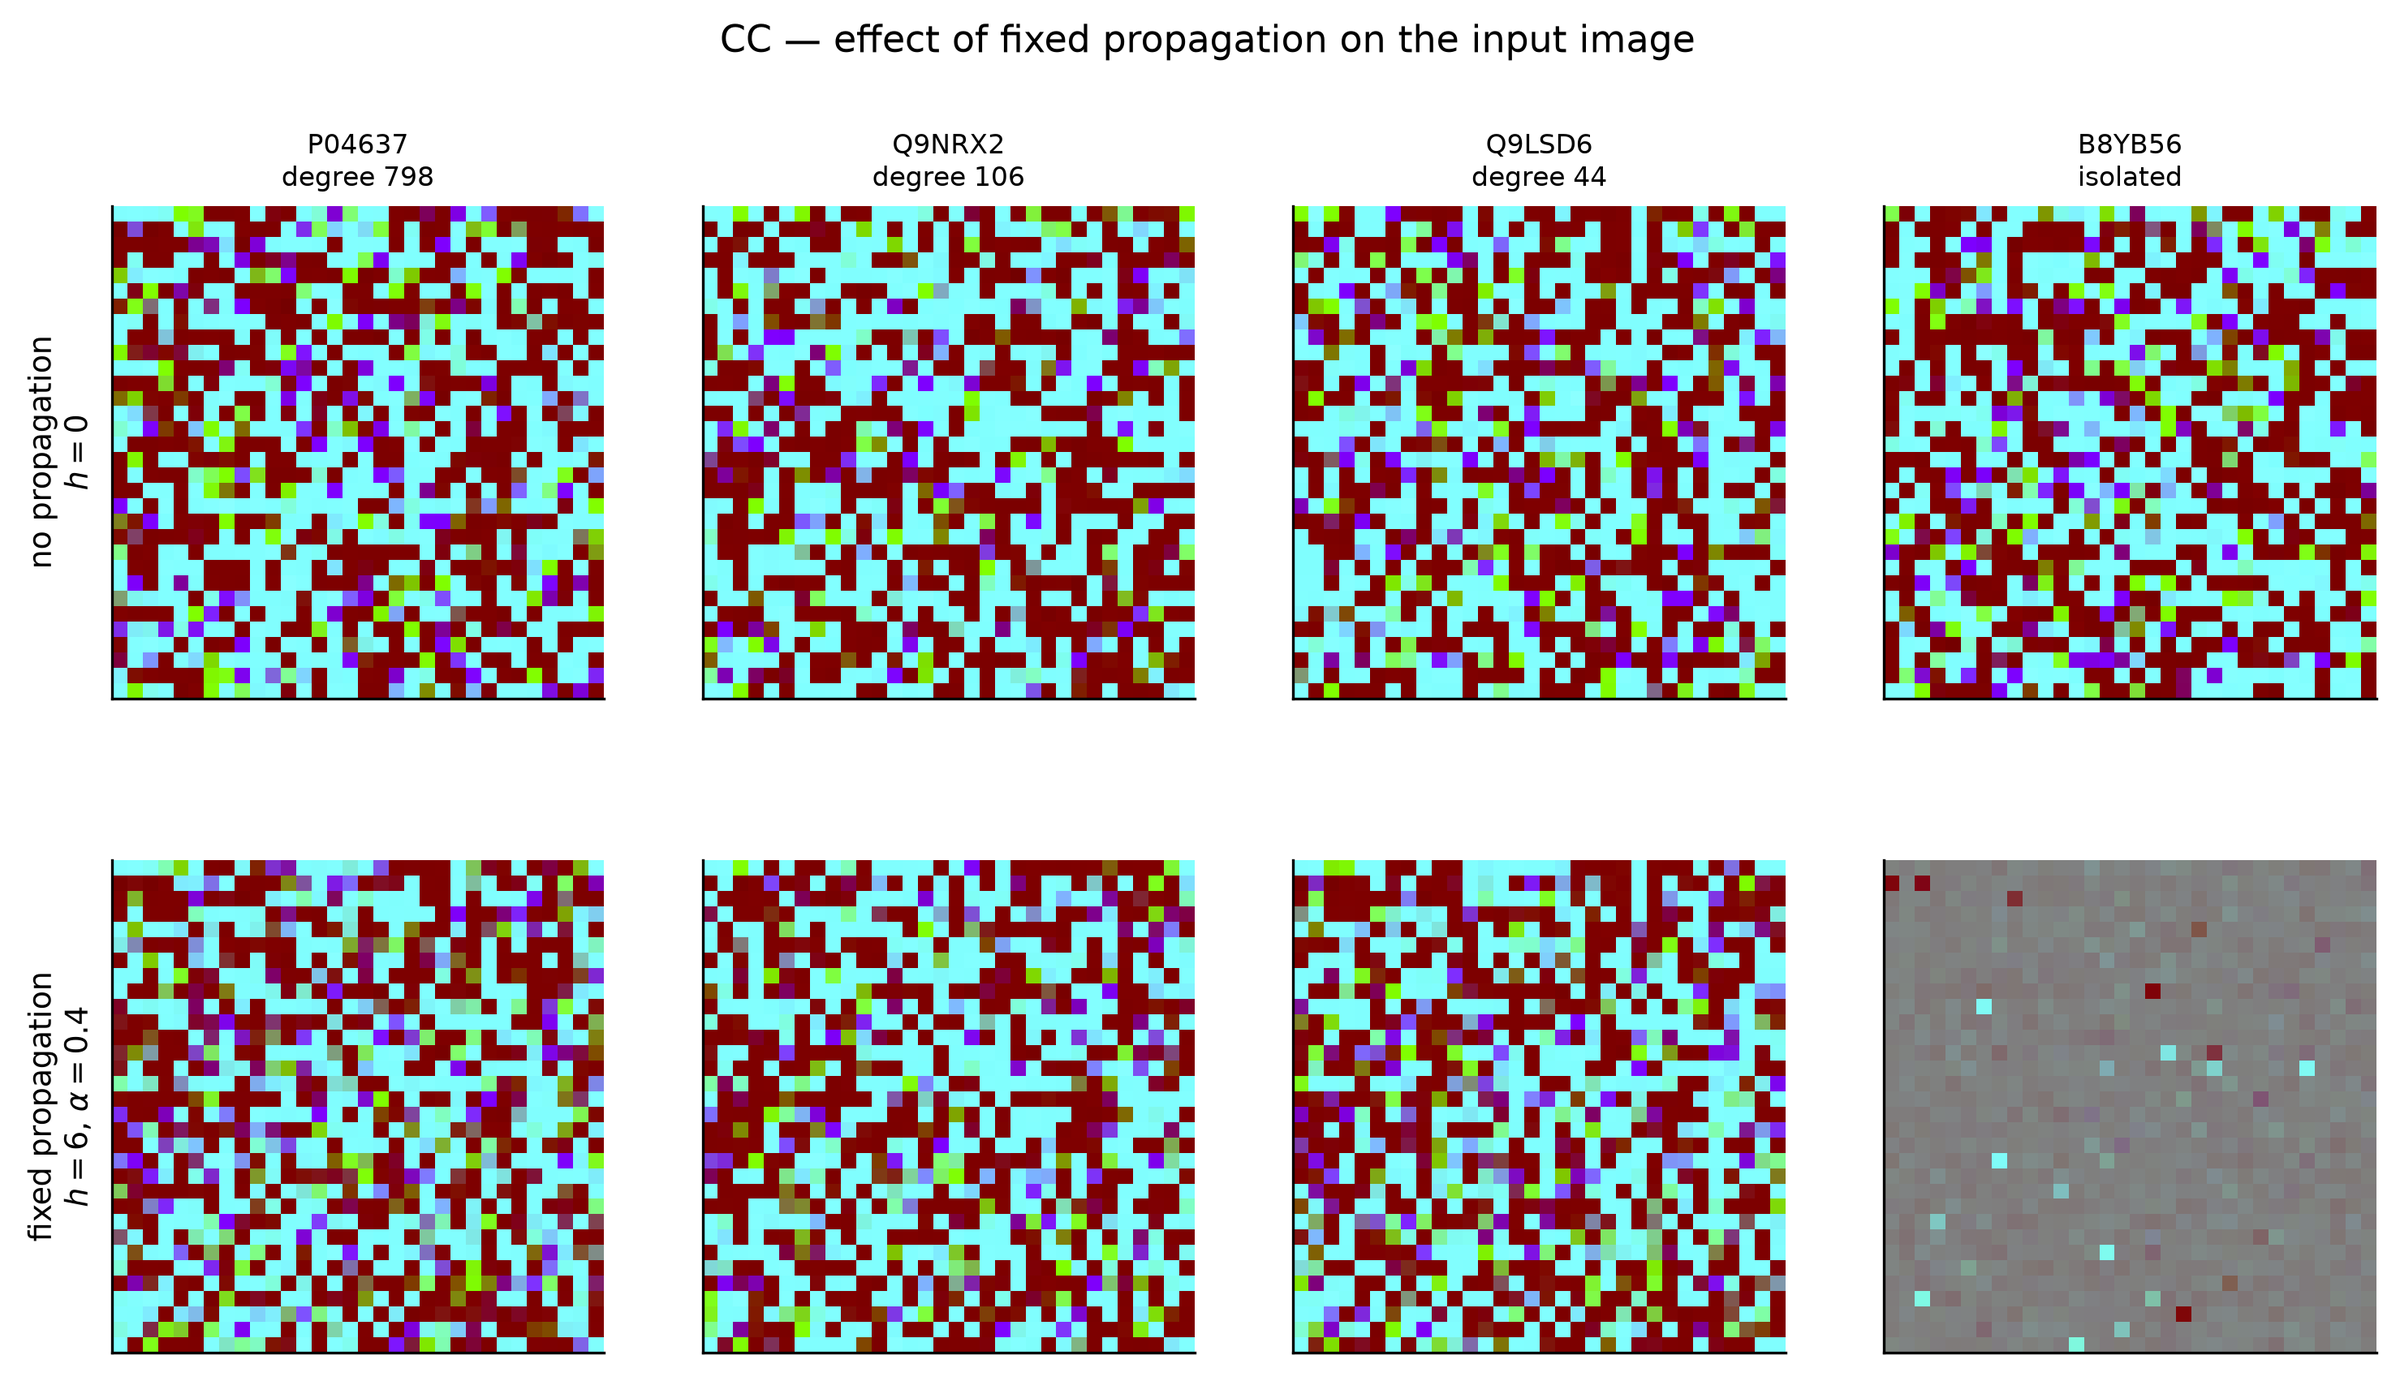
\includegraphics[width=896.7\px,height=514.5\px]{figures/fig_5_8.png}};
\node[tl] at (88,70) {\fmR\fz{16}{16}\color{inkii}\ls{2}\Ll{4 · Method}};
\node[tl] at (88,131) {\fdA\fz{54}{56.7}\color{ink}\ls{-1}\Ll{Propagation on four real proteins}};
\node<2-4>[tl] at (88,787.5) {\fmR\fz{15}{19.5}\color{muted}\Ll{Dissertation, Fig. 5.8 · CC, top {\fz{17.5}{21}$T = 0$}, bottom {\fz{17.5}{21}$T = 6,\ \alpha = 0.4$}}};
\node<3-4>[tl] at (1094.7,232) {\fbR\fz{26}{35.1}\color{ink}\Ll{Connected proteins keep their\\structure and absorb their\\neighbourhood}};
\node<4>[tl] at (1094.7,353.3) {\fbR\fz{26}{35.1}\color{ink}\Ll{An isolated protein becomes\\{\fz{29.2}{35}$\alpha^{T} \mathbf{H}^{(0)}$}: same direction,\\smaller scale}};
\node<4>[tl] at (1094.7,474.6) {\fbR\fz{26}{35.1}\color{ink}\Ll{So degree-zero gains cannot come\\from neighbourhood information}};
\node[tr] at (1512,876) {\fmR\fz{16}{16}\color{muted}25 / 45};
\end{tikzpicture}
\note{The rescaling is a structural property of the operator, not a tuned setting. 

The learned route adds self-loops and never mixes an isolated node with others.}
\end{frame}

\begin{frame}[plain]
\begin{tikzpicture}[deck]
\node<1>[box] at (0,0) {\includegraphics[page=3,width=1600\px]{build/layers}};
\node<2>[box] at (0,0) {\includegraphics[page=70,width=1600\px]{build/layers}};
\node<3>[box] at (0,0) {\includegraphics[page=82,width=1600\px]{build/layers}};
\node<4>[box] at (0,0) {\includegraphics[page=83,width=1600\px]{build/layers}};
\node<5>[box] at (0,0) {\includegraphics[page=84,width=1600\px]{build/layers}};
\node[tl] at (88,70) {\fmR\fz{16}{16}\color{inkii}\ls{2}\Ll{4 · Method}};
\node[tl] at (88,131) {\fdA\fz{54}{56.7}\color{ink}\ls{-1}\Ll{Learned propagation: GCN and GAT}};
\node<2-5>[tl] at (124,236) {\fbR\fz{30}{40.5}\color{ink}\Ll{GCN: symmetric normalization of\\{\fz{33.7}{40.4}$W + I$}, then a trained transform}};
\node<3-5>[tl] at (124,339) {\fbR\fz{30}{40.5}\color{ink}\Ll{GAT: attention over neighbours, 4 heads,\\edge score as attribute}};
\node<4-5>[tl] at (124,442) {\fbR\fz{30}{40.5}\color{ink}\Ll{2 layers, width 1024, output {\fz{33.7}{40.4}$\mathbf{g} \in \mathbb{R}^{1024}$}\\for the head}};
\node<5>[tl] at (124,545) {\fbR\fz{30}{40.5}\color{ink}\Ll{Full-graph forward on every step: about\\289 propagations per epoch}};
\node<2-5>[tl] at (694.7,220) {\fmR\fz{16}{16}\color{inkii}\Ll{GCN}};
\node<2-5>[tl] at (694.7,268.1) {\fbR\fz{28}{33.6}\color{ink}\Ll{{\fz{31.4}{37.7}$\displaystyle \mathbf{H}^{(\ell+1)} = \phi\!\left( \tilde{D}^{-1/2}\,\tilde{W}\,\tilde{D}^{-1/2}\,\mathbf{H}^{(\ell)}\,\Theta^{(\ell)} \right), \quad \tilde{W} = W + I$}}};
\node<3-5>[tl] at (694.7,336.5) {\fmR\fz{16}{16}\color{inkii}\Ll{GAT}};
\node<3-5>[tl] at (694.7,376.3) {\fbR\fz{28}{33.6}\color{ink}\Ll{{\fz{31.4}{37.7}$\displaystyle e_{ij} = \operatorname{LeakyReLU}\!\left( \mathbf{q}^{\top} \left[\, \Theta \mathbf{h}_i \,\|\, \Theta \mathbf{h}_j \,\|\, \Theta_e\, w_{ij} \,\right] \right)$}}};
\node<3-5>[tl] at (694.7,446.6) {\fbR\fz{28}{33.6}\color{ink}\Ll{{\fz{31.4}{37.7}$\displaystyle a_{ij} = \frac{\exp(e_{ij})}{\sum_{k \in \mathcal{N}(i) \cup \{i\}} \exp(e_{ik})}$}}};
\node<5>[tl] at (694.7,539.4) {\fbR\fz{22}{26.4}\color{inkii}\Ll{fixed}};
\node<5>[tl] at (862.7,570.4) {\fbR\fz{20}{27}\color{inkii}\Ll{computed once}};
\node<5>[tl] at (694.7,609.4) {\fbR\fz{22}{26.4}\color{inkii}\Ll{learned}};
\node<5>[tl] at (862.7,640.4) {\fbR\fz{20}{27}\color{inkii}\Ll{recomputed every optimization step}};
\node[tr] at (1512,876) {\fmR\fz{16}{16}\color{muted}26 / 45};
\end{tikzpicture}
\note{The GCN takes the STRING confidence as an edge weight; the GAT re-estimates it. 

Exact propagation with a mini-batch loss forces a full-graph pass for every batch, which is where the cost comes from.}
\end{frame}

\begin{frame}[plain]
\begin{tikzpicture}[deck]
\node<1>[box] at (0,0) {\includegraphics[page=3,width=1600\px]{build/layers}};
\node<2>[box] at (0,0) {\includegraphics[page=85,width=1600\px]{build/layers}};
\node<3>[box] at (0,0) {\includegraphics[page=86,width=1600\px]{build/layers}};
\node<4>[box] at (0,0) {\includegraphics[page=87,width=1600\px]{build/layers}};
\node<5>[box] at (0,0) {\includegraphics[page=88,width=1600\px]{build/layers}};
\node<3-5>[box] at (109,235) {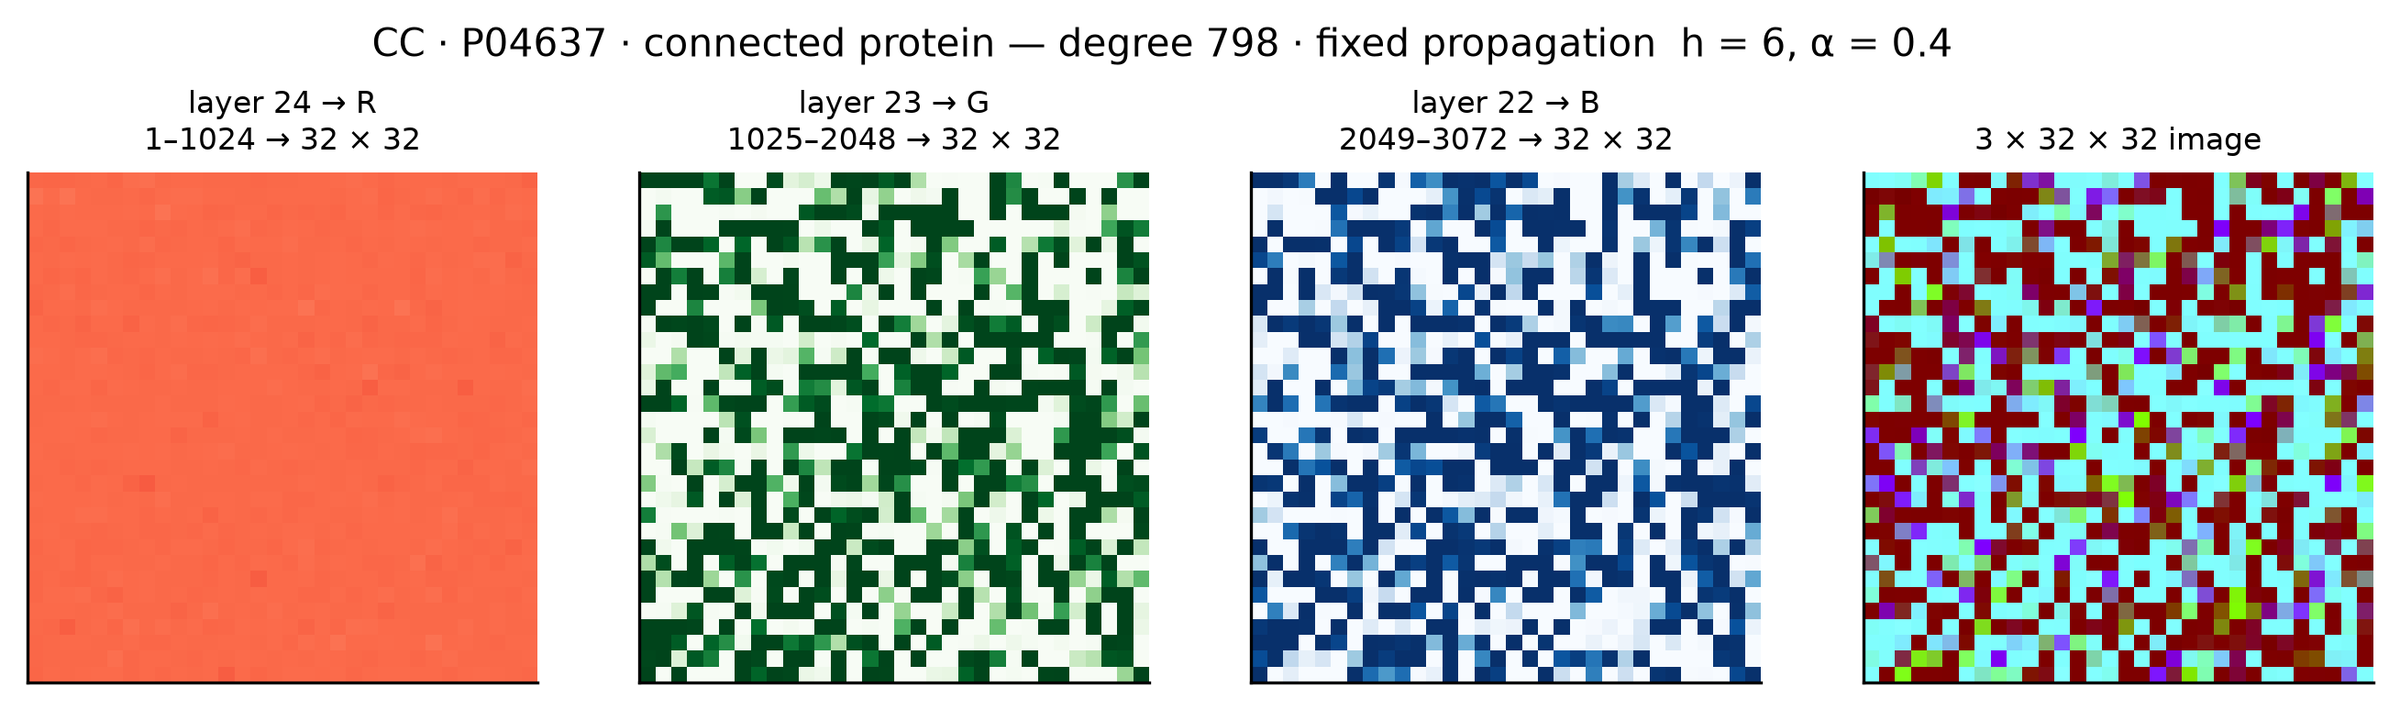
\includegraphics[width=1115.5\px,height=330\px]{figures/fig_5_9.png}};
\node[tl] at (88,70) {\fmR\fz{16}{16}\color{inkii}\ls{2}\Ll{4 · Method}};
\node[tl] at (88,131) {\fdA\fz{54}{56.7}\color{ink}\ls{-1}\Ll{Vector head and vision head}};
\node<3-5>[tl] at (88,603) {\fmR\fz{15}{19.5}\color{muted}\Ll{Dissertation, Fig. 5.9}};
\node<2-5>[tl] at (124,657.5) {\fbR\fz{26}{35.1}\color{ink}\Ll{Vector: MLP [1024, 512], batch norm, dropout 0.4}};
\node<4-5>[tl] at (856,657.5) {\fbR\fz{26}{35.1}\color{ink}\Ll{Backbones: ResNet-50 and ConvNeXt-Tiny (ImageNet),\\fully fine-tuned}};
\node<3-5>[tl] at (124,759.8) {\fbR\fz{26}{35.1}\color{ink}\Ll{Vision: {\fz{29.2}{35}$\sigma(\mathrm{clip}(z))$} split into three 32 × 32 channels, one\\per ProtT5 layer}};
\node<5>[tl] at (856,759.8) {\fbR\fz{26}{35.1}\color{ink}\Ll{Caution: pixel adjacency has no meaning here}};
\node[tr] at (1512,876) {\fmR\fz{16}{16}\color{muted}27 / 45};
\end{tikzpicture}
\note{The image is built inside the forward pass and never written to disk. 

Neighbouring pixels are neighbouring embedding coordinates only by storage order, a caveat that the results confirm.}
\end{frame}

\begin{frame}[plain]
\begin{tikzpicture}[deck]
\node<1-2>[box] at (0,0) {\includegraphics[page=3,width=1600\px]{build/layers}};
\node<3>[box] at (0,0) {\includegraphics[page=89,width=1600\px]{build/layers}};
\node<4>[box] at (0,0) {\includegraphics[page=90,width=1600\px]{build/layers}};
\node<5>[box] at (0,0) {\includegraphics[page=91,width=1600\px]{build/layers}};
\node[tl] at (88,70) {\fmR\fz{16}{16}\color{inkii}\ls{2}\Ll{4 · Method}};
\node[tl] at (88,131) {\fdA\fz{54}{56.7}\color{ink}\ls{-1}\Ll{Training objective: ProteinLoss}};
\node<2-5>[tl] at (88,251.7) {\fbR\fz{44}{52.8}\color{ink}\Ll{{\fz{49.4}{59.2}$\displaystyle \mathcal{L} = \mathcal{L}_{\text{ZLPR}} \cdot \bigl(1 - \mathrm{wF}_1^{\text{GO}}\bigr) \cdot \bigl(1 - \mathrm{wF}_1^{\text{prot}}\bigr)$}}};
\node<3-5>[tl] at (124,335) {\fbR\fz{30}{40.5}\color{ink}\Ll{ZLPR separates positive from negative\\terms at threshold zero}};
\node<4-5>[tl] at (124,438) {\fbR\fz{30}{40.5}\color{ink}\Ll{Two soft, IC-weighted {\fz{33.7}{40.4}$F_1$} factors: one\\across terms, one across proteins}};
\node<5>[tl] at (124,541) {\fbR\fz{30}{40.5}\color{ink}\Ll{Brings training closer to the\\evaluation criterion}};
\node[tr] at (1512,876) {\fmR\fz{16}{16}\color{muted}28 / 45};
\end{tikzpicture}
\note{Inherited from InterLabelGO+ through the group's sequence-only line. 

It beats binary cross-entropy by 5.47 pp on the first-generation mean, so every later run uses it.}
\end{frame}

\begin{frame}[plain]
\begin{tikzpicture}[deck]
\node<1>[box] at (0,0) {\includegraphics[page=3,width=1600\px]{build/layers}};
\node<2>[box] at (0,0) {\includegraphics[page=92,width=1600\px]{build/layers}};
\node<3>[box] at (0,0) {\includegraphics[page=93,width=1600\px]{build/layers}};
\node<4>[box] at (0,0) {\includegraphics[page=94,width=1600\px]{build/layers}};
\node<5>[box] at (0,0) {\includegraphics[page=95,width=1600\px]{build/layers}};
\node<6>[box] at (0,0) {\includegraphics[page=96,width=1600\px]{build/layers}};
\node<2-6>[box] at (109,235) {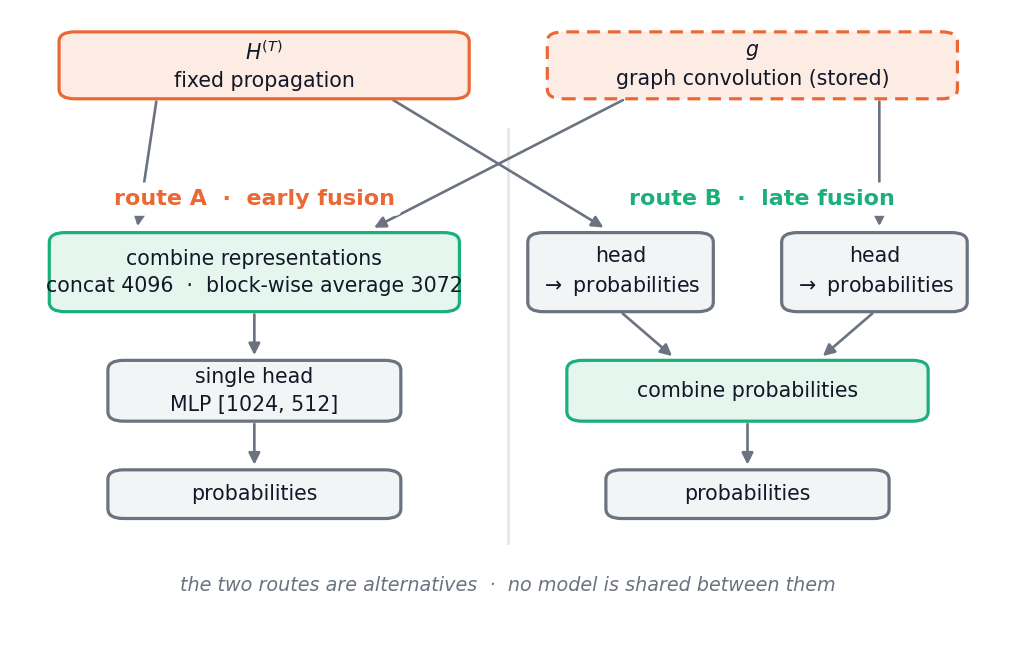
\includegraphics[width=654\px,height=417.1\px]{figures/fig_5_10.png}};
\node[tl] at (88,70) {\fmR\fz{16}{16}\color{inkii}\ls{2}\Ll{4 · Method}};
\node[tl] at (88,131) {\fdA\fz{54}{56.7}\color{ink}\ls{-1}\Ll{Combining the fixed and learned routes}};
\node<2-6>[tl] at (88,690.1) {\fmR\fz{15}{19.5}\color{muted}\Ll{Dissertation, Fig. 5.10}};
\node<3-6>[tl] at (852,232) {\fbR\fz{26}{35.1}\color{ink}\Ll{Early: join representations, train one head (concat 4096\\or block-wise add 3072)}};
\node<4-6>[tl] at (852,318.2) {\fbR\fz{26}{35.1}\color{ink}\Ll{Late: train each route, combine probabilities}};
\node<5-6>[tl] at (852,369.3) {\fbR\fz{26}{35.1}\color{ink}\Ll{Eleven late rules: linear {\fz{29.2}{35}$\gamma$}, max, min, IC sigmoid, degree\\sigmoid, master equation, five stacking meta-classifiers}};
\node<6>[tl] at (852,455.5) {\fbR\fz{26}{35.1}\color{ink}\Ll{Coefficients chosen on validation (71 configurations\\per ontology)}};
\node[tr] at (1512,876) {\fmR\fz{16}{16}\color{muted}29 / 45};
\end{tikzpicture}
\note{The two routes are alternatives, no model is shared. 

Early fusion lets one head learn how to weigh the sources; late fusion leaves each route to its own optimization and needs no training to combine.}
\end{frame}

\section{5 · Results}
\begin{frame}[plain]
\begin{tikzpicture}[deck]
\node<1>[box] at (0,0) {\includegraphics[page=3,width=1600\px]{build/layers}};
\node<2>[box] at (0,0) {\includegraphics[page=7,width=1600\px]{build/layers}};
\node<3>[box] at (0,0) {\includegraphics[page=97,width=1600\px]{build/layers}};
\node<4>[box] at (0,0) {\includegraphics[page=98,width=1600\px]{build/layers}};
\node[tl] at (88,70) {\fmR\fz{16}{16}\color{inkii}\ls{2}\Ll{5 · Results}};
\node[tl] at (88,131) {\fdA\fz{54}{56.7}\color{ink}\ls{-1}\Ll{170 runs, one funnel}};
\node<2-4>[tl] at (124,236) {\fbR\fz{30}{40.5}\color{ink}\Ll{170 runs, about 136.3 GPU-\\hours (147 on an RTX A5500)}};
\node<3-4>[tl] at (612,236) {\fbR\fz{30}{40.5}\color{ink}\Ll{Each stage picks its winner on\\validation and hands it on}};
\node<4>[tl] at (1100,236) {\fbR\fz{30}{40.5}\color{ink}\Ll{Test read once, at the end}};
\node[tr] at (1512,876) {\fmR\fz{16}{16}\color{muted}30 / 45};
\end{tikzpicture}
\note{The selection never touches the test partition. Every reported test number is a single evaluation of a frozen configuration. 

Two stations are not pure validation picks: max deduplication rests on an analytic argument (all 170 runs use it; the sum figures come from the earlier campaign), and ConvNeXt-Tiny is carried forward on a 0.57 pp margin plus the VISAPP campaign.}
\end{frame}

\begin{frame}[plain]
\begin{tikzpicture}[deck]
\node<1>[box] at (0,0) {\includegraphics[page=99,width=1600\px]{build/layers}};
\node<2>[box] at (0,0) {\includegraphics[page=100,width=1600\px]{build/layers}};
\node<3>[box] at (0,0) {\includegraphics[page=101,width=1600\px]{build/layers}};
\node<4>[box] at (0,0) {\includegraphics[page=102,width=1600\px]{build/layers}};
\node<5>[box] at (0,0) {\includegraphics[page=103,width=1600\px]{build/layers}};
\node[tl] at (88,70) {\fmR\fz{16}{16}\color{inkii}\ls{2}\Ll{5 · Results}};
\node[tl] at (88,131) {\fdA\fz{54}{56.7}\color{ink}\ls{-1}\Ll{Generation 1 settles three choices}};
\node<2-5>[tl] at (124,232) {\fbR\fz{26}{35.1}\color{ink}\Ll{Naive term-frequency baseline: 43.56\\mean wF\textsubscript{max}}};
\node<3-5>[tl] at (124,318.2) {\fbR\fz{26}{35.1}\color{ink}\Ll{ProteinLoss beats binary cross-entropy: +5.47\\pp mean (+8.87 in MF)}};
\node<4-5>[tl] at (124,404.4) {\fbR\fz{26}{35.1}\color{ink}\Ll{MLP on the raw profile wins: 44.51; best 1-D\\CNN 41.16}};
\node<5>[tl] at (124,490.6) {\fbR\fz{26}{35.1}\color{ink}\Ll{Vision backbones: 36.99 to 37.62}};
\node[tr] at (1512,876) {\fmR\fz{16}{16}\color{muted}31 / 45};
\end{tikzpicture}
\note{Topology alone barely clears a predictor that looks at nothing: 0.95 pp on the mean, and below it in BP. 

The vector route wins, and ConvNeXt-Tiny is carried forward on a 0.57 pp margin plus the earlier VISAPP campaign.}
\end{frame}

\begin{frame}[plain]
\begin{tikzpicture}[deck]
\node<1>[box] at (0,0) {\includegraphics[page=3,width=1600\px]{build/layers}};
\node<2>[box] at (0,0) {\includegraphics[page=104,width=1600\px]{build/layers}};
\node<3>[box] at (0,0) {\includegraphics[page=105,width=1600\px]{build/layers}};
\node<4>[box] at (0,0) {\includegraphics[page=106,width=1600\px]{build/layers}};
\node<2-4>[box] at (159.6,235) {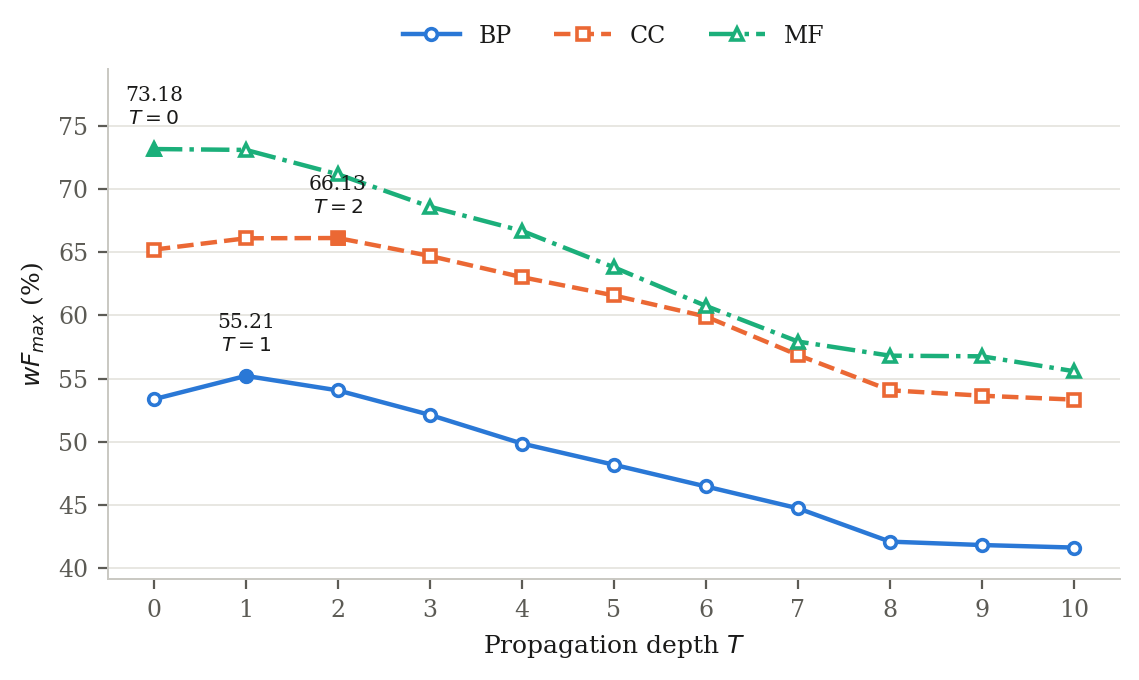
\includegraphics[width=552.8\px,height=330\px]{figures/fig_6_1.png}};
\node<3-4>[box] at (887.6,235) {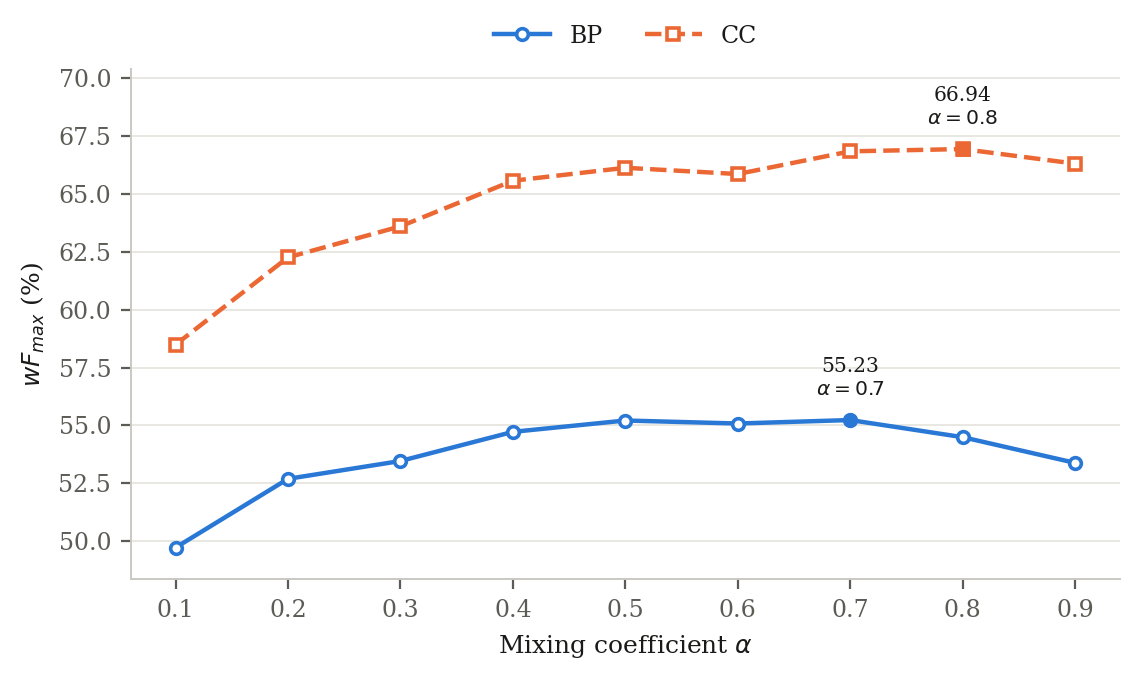
\includegraphics[width=552.8\px,height=330\px]{figures/fig_6_2.png}};
\node[tl] at (88,70) {\fmR\fz{16}{16}\color{inkii}\ls{2}\Ll{5 · Results}};
\node[tl] at (88,131) {\fdA\fz{54}{56.7}\color{ink}\ls{-1}\Ll{One or two hops, high retention}};
\node<2-4>[tl] at (88,603) {\fmR\fz{15}{19.5}\color{muted}\Ll{Dissertation, Fig. 6.1 · vector head, depth, validation}};
\node<3-4>[tl] at (816,603) {\fmR\fz{15}{19.5}\color{muted}\Ll{Dissertation, Fig. 6.2 · vector head, retention, validation}};
\node<2-4>[tl] at (124,655.5) {\fbR\fz{26}{35.1}\color{ink}\Ll{Peak depth: {\fz{29.2}{35}$T = 1$} BP, {\fz{29.2}{35}$T = 2$} CC, {\fz{29.2}{35}$T = 0$} MF}};
\node<3-4>[tl] at (852,655.5) {\fbR\fz{26}{35.1}\color{ink}\Ll{Best retention: {\fz{29.2}{35}$\alpha = 0.7$} BP, {\fz{29.2}{35}$\alpha = 0.8$} CC}};
\node<2-4>[tl] at (124,741.2) {\fbR\fz{26}{35.1}\color{ink}\Ll{Beyond the peak, performance falls 12.80 to 17.60 pp\\by {\fz{29.2}{35}$T = 10$}}};
\node<4>[tl] at (852,741.2) {\fbR\fz{26}{35.1}\color{ink}\Ll{The graph corrects the protein's own representation; it\\does not replace it}};
\node[tr] at (1512,876) {\fmR\fz{16}{16}\color{muted}32 / 45};
\end{tikzpicture}
\note{In MF no amount of propagation helps; the best configuration switches the graph off. 

In CC everything below $\alpha$ = 0.4 is worse than everything above it; in BP the single exception is $\alpha$ = 0.9.}
\end{frame}

\begin{frame}[plain]
\begin{tikzpicture}[deck]
\node<1>[box] at (0,0) {\includegraphics[page=3,width=1600\px]{build/layers}};
\node<2>[box] at (0,0) {\includegraphics[page=107,width=1600\px]{build/layers}};
\node<3>[box] at (0,0) {\includegraphics[page=108,width=1600\px]{build/layers}};
\node<4>[box] at (0,0) {\includegraphics[page=109,width=1600\px]{build/layers}};
\node<2-4>[box] at (159.6,235) {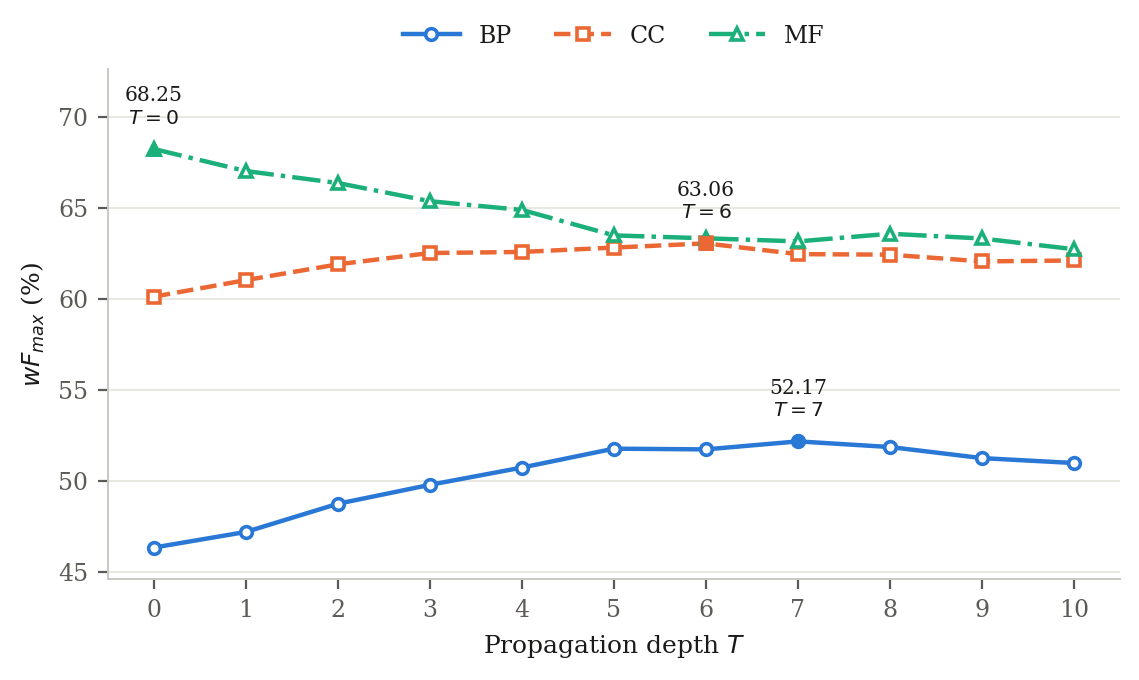
\includegraphics[width=552.8\px,height=330\px]{figures/fig_6_3.png}};
\node<3-4>[box] at (887.6,235) {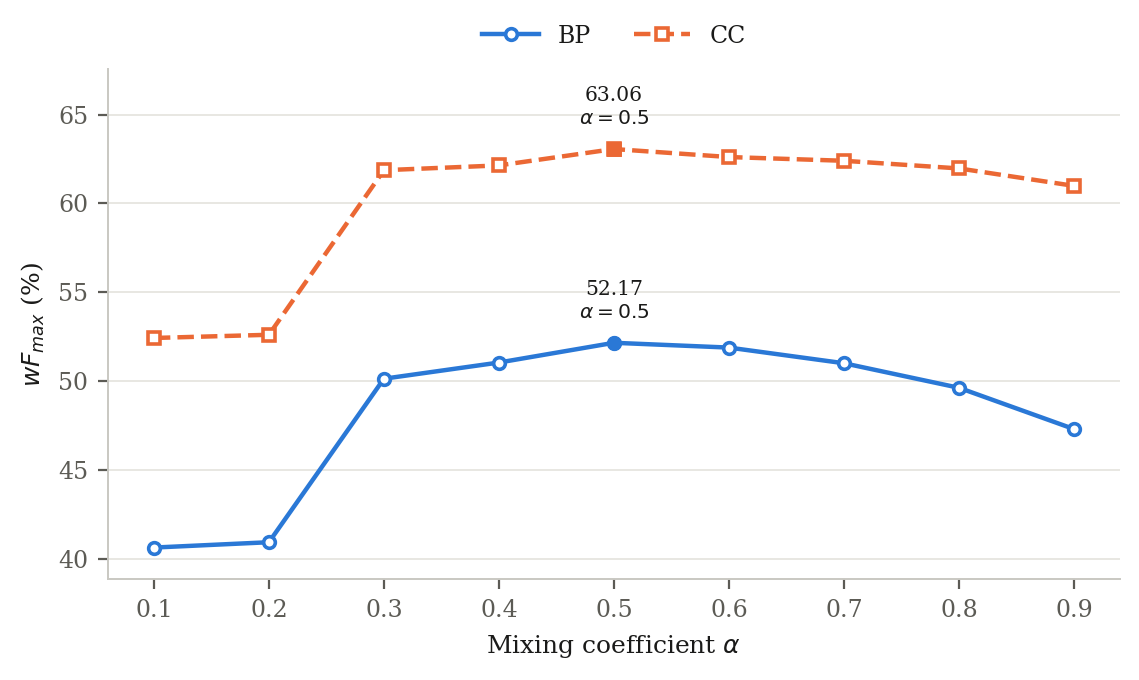
\includegraphics[width=552.8\px,height=330\px]{figures/fig_6_4.png}};
\node[tl] at (88,70) {\fmR\fz{16}{16}\color{inkii}\ls{2}\Ll{5 · Results}};
\node[tl] at (88,131) {\fdA\fz{54}{56.7}\color{ink}\ls{-1}\Ll{The vision head wants deep propagation}};
\node<2-4>[tl] at (88,603) {\fmR\fz{15}{19.5}\color{muted}\Ll{Dissertation, Fig. 6.3 · vision head, depth, validation}};
\node<3-4>[tl] at (816,603) {\fmR\fz{15}{19.5}\color{muted}\Ll{Dissertation, Fig. 6.4 · vision head, retention, validation}};
\node<2-4>[tl] at (124,655.5) {\fbR\fz{26}{35.1}\color{ink}\Ll{Peak depth: {\fz{29.2}{35}$T = 7$} BP, {\fz{29.2}{35}$T = 6$} CC, {\fz{29.2}{35}$T = 0$} MF; a plateau,\\not a peak}};
\node<3-4>[tl] at (852,655.5) {\fbR\fz{26}{35.1}\color{ink}\Ll{Collapse at {\fz{29.2}{35}$\alpha \le 0.2$}: isolated nodes shrink as {\fz{29.2}{35}$\alpha^{T}$} ({\fz{29.2}{35}$10^{-7}$}\\at {\fz{29.2}{35}$T = 7$})}};
\node<2-4>[tl] at (124,758.8) {\fbR\fz{26}{35.1}\color{ink}\Ll{Gains over {\fz{29.2}{35}$T = 0$}: +5.84 BP, +2.93 CC (vector head:\\+1.85, +0.92)}};
\node<4>[tl] at (852,758.8) {\fbR\fz{26}{35.1}\color{ink}\Ll{Its best BP value, 52.17, is still below the vector head's\\graph-free 53.36}};
\node[tr] at (1512,876) {\fmR\fz{16}{16}\color{muted}33 / 45};
\end{tikzpicture}
\note{The vision head extracts less from the node itself, so dilution costs it less and the neighbourhood average helps more. 

MF peaks at T = 0 in both heads, the strongest form of that observation.}
\end{frame}

\begin{frame}[plain]
\begin{tikzpicture}[deck]
\node<1>[box] at (0,0) {\includegraphics[page=110,width=1600\px]{build/layers}};
\node<2>[box] at (0,0) {\includegraphics[page=111,width=1600\px]{build/layers}};
\node<3>[box] at (0,0) {\includegraphics[page=112,width=1600\px]{build/layers}};
\node<4>[box] at (0,0) {\includegraphics[page=113,width=1600\px]{build/layers}};
\node<5>[box] at (0,0) {\includegraphics[page=114,width=1600\px]{build/layers}};
\node[tl] at (88,70) {\fmR\fz{16}{16}\color{inkii}\ls{2}\Ll{5 · Results}};
\node[tl] at (88,131) {\fdA\fz{54}{56.7}\color{ink}\ls{-1}\Ll{Learning the aggregation does not pay}};
\node<2-5>[tl] at (124,232) {\fbR\fz{26}{35.1}\color{ink}\Ll{GCN beats GAT in all 6 pairs (3.88 to 9.31 pp),\\and in 30 of 30 fusion pairs}};
\node<3-5>[tl] at (124,318.2) {\fbR\fz{26}{35.1}\color{ink}\Ll{Fixed 65.12 vs GCN 63.32 mean wF\textsubscript{max}}};
\node<4-5>[tl] at (124,369.3) {\fbR\fz{26}{35.1}\color{ink}\Ll{GCN ahead in BP by 0.55 (a tie); behind in CC\\by 0.59 and MF by 5.35}};
\node<5>[tl] at (124,455.5) {\fbR\fz{26}{35.1}\color{ink}\Ll{Deduplication: max never loses beyond noise;\\GAT gains most (+3.83 vision)}};
\node[tr] at (1512,876) {\fmR\fz{16}{16}\color{muted}34 / 45};
\end{tikzpicture}
\note{Attention does not recover a better weighting than the STRING score it was handed. 

A plausible reason: the loss is masked to training nodes, so attention parameters see gradient only through a two-hop receptive field.}
\end{frame}

\begin{frame}[plain]
\begin{tikzpicture}[deck]
\node<1>[box] at (0,0) {\includegraphics[page=115,width=1600\px]{build/layers}};
\node<2>[box] at (0,0) {\includegraphics[page=116,width=1600\px]{build/layers}};
\node<3>[box] at (0,0) {\includegraphics[page=117,width=1600\px]{build/layers}};
\node<4>[box] at (0,0) {\includegraphics[page=118,width=1600\px]{build/layers}};
\node<5>[box] at (0,0) {\includegraphics[page=119,width=1600\px]{build/layers}};
\node[tl] at (88,70) {\fmR\fz{16}{16}\color{inkii}\ls{2}\Ll{5 · Results}};
\node[tl] at (88,131) {\fdA\fz{54}{56.7}\color{ink}\ls{-1}\Ll{Fusion helps; combining predictions helps more}};
\node<2-5>[tl] at (124,232) {\fbR\fz{26}{35.1}\color{ink}\Ll{Early, one configuration (add, GCN, vector):\\65.80, +0.68 over fixed alone}};
\node<3-5>[tl] at (124,318.2) {\fbR\fz{26}{35.1}\color{ink}\Ll{Late, linear {\fz{29.2}{35}$\gamma$} (0.50 BP, 0.55 CC and MF):\\67.06, best in every ontology}};
\node<4-5>[tl] at (124,404.4) {\fbR\fz{26}{35.1}\color{ink}\Ll{Gains over the better component: +2.18 BP,\\+1.85 CC, +1.26 MF}};
\node<5>[tl] at (124,490.6) {\fbR\fz{26}{35.1}\color{ink}\Ll{Stacking importances: the two probabilities\\carry almost all the weight}};
\node[tr] at (1512,876) {\fmR\fz{16}{16}\color{muted}35 / 45};
\end{tikzpicture}
\note{A single scalar beats every elaborate rule, including gradient boosting. The auxiliary features do not predict which route is right, and the conditional rules converged to the flattest sigmoid in the grid. 

The ensemble fits one extra parameter on validation.}
\end{frame}

\begin{frame}[plain]
\begin{tikzpicture}[deck]
\node<1>[box] at (0,0) {\includegraphics[page=120,width=1600\px]{build/layers}};
\node<2>[box] at (0,0) {\includegraphics[page=121,width=1600\px]{build/layers}};
\node<3>[box] at (0,0) {\includegraphics[page=122,width=1600\px]{build/layers}};
\node<4>[box] at (0,0) {\includegraphics[page=123,width=1600\px]{build/layers}};
\node[tl] at (88,70) {\fmR\fz{16}{16}\color{inkii}\ls{2}\Ll{5 · Results}};
\node[tl] at (88,131) {\fdA\fz{54}{56.7}\color{ink}\ls{-1}\Ll{Vector head wins 12 of 12}};
\node<3-4>[tl] at (1094.7,232) {\fbR\fz{26}{35.1}\color{ink}\Ll{Margin on the mean: +6.62,\\+3.96, +2.69, +3.35 pp across the\\four stages}};
\node<3-4>[tl] at (1094.7,353.3) {\fbR\fz{26}{35.1}\color{ink}\Ll{No trend toward zero}};
\node<4>[tl] at (1094.7,404.4) {\fbR\fz{26}{35.1}\color{ink}\Ll{Neither image has the locality a\\convolution assumes}};
\node[tr] at (1512,876) {\fmR\fz{16}{16}\color{muted}36 / 45};
\end{tikzpicture}
\note{Generation 1 images index arbitrary training proteins; generation 2 images reshape embedding coordinates. 

Three independent pieces of evidence agree: pooling order, the 1-D CNN failure and this table.}
\end{frame}

\begin{frame}[plain]
\begin{tikzpicture}[deck]
\node<1>[box] at (0,0) {\includegraphics[page=124,width=1600\px]{build/layers}};
\node<2>[box] at (0,0) {\includegraphics[page=125,width=1600\px]{build/layers}};
\node<3>[box] at (0,0) {\includegraphics[page=126,width=1600\px]{build/layers}};
\node<4>[box] at (0,0) {\includegraphics[page=127,width=1600\px]{build/layers}};
\node<5>[box] at (0,0) {\includegraphics[page=128,width=1600\px]{build/layers}};
\node[tl] at (88,70) {\fmR\fz{16}{16}\color{inkii}\ls{2}\Ll{5 · Results}};
\node[tl] at (88,131) {\fdA\fz{54}{56.7}\color{ink}\ls{-1}\Ll{Where the gains come from}};
\node<4-5>[tl] at (124,688) {\fbR\fz{26}{35.1}\color{ink}\Ll{Mean validation wF\textsubscript{max}: Naive 43.56 $\rightarrow$ Generation 1 44.51 $\rightarrow$ ProtT5 alone 63.92 $\rightarrow$ Fixed 65.12 $\rightarrow$ Early 65.84 $\rightarrow$\\Late 67.06}};
\node<5>[tl] at (124,774.2) {\fbR\fz{26}{35.1}\color{ink}\Ll{Most of the jump is the language model; the graph adds the rest}};
\node[tr] at (1512,876) {\fmR\fz{16}{16}\color{muted}37 / 45};
\end{tikzpicture}
\note{This is the whole dissertation on one axis. The protein language model explains most of the distance, and the graph contributes a consistent remainder in BP and CC. 

Each value is a mean of per-ontology champions on validation; the learned GNN alone, 63.32, sits below the ProtT5 control because of MF, so it is not a step of the staircase.}
\end{frame}

\begin{frame}[plain]
\hypertarget<1>{s38.1}{}
\hypertarget<2>{s38.2}{}
\hypertarget<3>{s38.3}{}
\hypertarget<4>{s38.4}{}
\hypertarget<5>{s38.5}{}
\hypertarget<6>{s38.6}{}
\hypertarget<7>{s38.7}{}
\begin{tikzpicture}[deck]
\node<1>[box] at (0,0) {\includegraphics[page=129,width=1600\px]{build/layers}};
\node<2>[box] at (0,0) {\includegraphics[page=130,width=1600\px]{build/layers}};
\node<3>[box] at (0,0) {\includegraphics[page=131,width=1600\px]{build/layers}};
\node<4>[box] at (0,0) {\includegraphics[page=132,width=1600\px]{build/layers}};
\node<5>[box] at (0,0) {\includegraphics[page=133,width=1600\px]{build/layers}};
\node<6>[box] at (0,0) {\includegraphics[page=134,width=1600\px]{build/layers}};
\node<7>[box] at (0,0) {\includegraphics[page=135,width=1600\px]{build/layers}};
\node<5>[box] at (787.5,208) {\hot{58.1}{42}{s38.5}};
\node<5>[box] at (844.1,208) {\hot{59.4}{42}{s38.6}};
\node<5>[box] at (902,208) {\hot{61.5}{42}{s38.7}};
\node<5>[box] at (1049.1,206) {\hot{227}{46}{s38x.4}};
\node<6>[box] at (787.5,208) {\hot{58.1}{42}{s38.5}};
\node<6>[box] at (844.1,208) {\hot{59.4}{42}{s38.6}};
\node<6>[box] at (902,208) {\hot{61.5}{42}{s38.7}};
\node<6>[box] at (1049.1,206) {\hot{227}{46}{s38x.10}};
\node<7>[box] at (787.5,208) {\hot{58.1}{42}{s38.5}};
\node<7>[box] at (844.1,208) {\hot{59.4}{42}{s38.6}};
\node<7>[box] at (902,208) {\hot{61.5}{42}{s38.7}};
\node<7>[box] at (1049.1,206) {\hot{227}{46}{s38x.16}};
\node[tl] at (88,70) {\fmR\fz{16}{16}\color{inkii}\ls{2}\Ll{5 · Results}};
\node[tl] at (88,131) {\fdA\fz{54}{56.7}\color{ink}\ls{-1}\Ll{Test set: NEXUS-GO vs five methods}};
\node<2-7>[tl] at (124,232) {\fbR\fz{26}{35.1}\color{ink}\Ll{NEXUS-GO/Late best in every column of the\\three tables, except AuPRC in MF}};
\node<3-7>[tl] at (124,318.2) {\fbR\fz{26}{35.1}\color{ink}\Ll{wF\textsubscript{max} margin over the strongest baseline:\\+9.77 BP, +8.67 CC, +4.93 MF}};
\node<4-7>[tl] at (124,404.4) {\fbR\fz{26}{35.1}\color{ink}\Ll{S\textsubscript{min}: 17.12 vs 20.11 (BP), 8.22 vs 9.67 (CC), 5.14\\vs 5.67 (MF)}};
\node<5-7>[tl] at (124,490.6) {\fbR\fz{26}{35.1}\color{ink}\Ll{The ProtT5 baseline alone already beats every\\literature method on wF\textsubscript{max}}};
\node[tr] at (1512,876) {\fmR\fz{16}{16}\color{muted}38 / 45};
\end{tikzpicture}
\note{Every baseline was retrained on the same corpus and scored with the same code. 

Three of them lose their multi-network mechanism on a single aggregated graph, so the ordering describes these adapted configurations, not the original papers.}
\end{frame}

\begin{frame}[plain]
\begin{tikzpicture}[deck]
\node<1>[box] at (0,0) {\includegraphics[page=136,width=1600\px]{build/layers}};
\node<2>[box] at (0,0) {\includegraphics[page=137,width=1600\px]{build/layers}};
\node<3>[box] at (0,0) {\includegraphics[page=138,width=1600\px]{build/layers}};
\node[tl] at (88,70) {\fmR\fz{16}{16}\color{inkii}\ls{2}\Ll{5 · Results}};
\node[tl] at (88,131) {\fdA\fz{54}{56.7}\color{ink}\ls{-1}\Ll{Every protein gets a prediction}};
\node<2-3>[tl] at (124,236) {\fbR\fz{30}{40.5}\color{ink}\Ll{NEXUS-GO: 100\% of the test partition in\\BP, CC, MF}};
\node<3>[tl] at (124,339) {\fbR\fz{30}{40.5}\color{ink}\Ll{DeepGraphGO and SEGT-GO: 95.1–\\96.3\% (homology search)}};
\node<3>[tl] at (124,442) {\fbR\fz{30}{40.5}\color{ink}\Ll{Mashup, MELISSA, deepNF: 63.6–68.7\%\\(network members only)}};
\node[tr] at (1512,876) {\fmR\fz{16}{16}\color{muted}39 / 45};
\end{tikzpicture}
\note{Missing proteins count as misses in the comparison, so part of the distance to the network-only methods is reach, not ranking quality. 

The proteins they cannot reach are exactly the band where sequence-aware routes score highest.}
\end{frame}

\begin{frame}[plain]
\begin{tikzpicture}[deck]
\node<1>[box] at (0,0) {\includegraphics[page=3,width=1600\px]{build/layers}};
\node<2>[box] at (0,0) {\includegraphics[page=139,width=1600\px]{build/layers}};
\node<3>[box] at (0,0) {\includegraphics[page=140,width=1600\px]{build/layers}};
\node<4>[box] at (0,0) {\includegraphics[page=141,width=1600\px]{build/layers}};
\node<5>[box] at (0,0) {\includegraphics[page=142,width=1600\px]{build/layers}};
\node<2-5>[box] at (109,235) {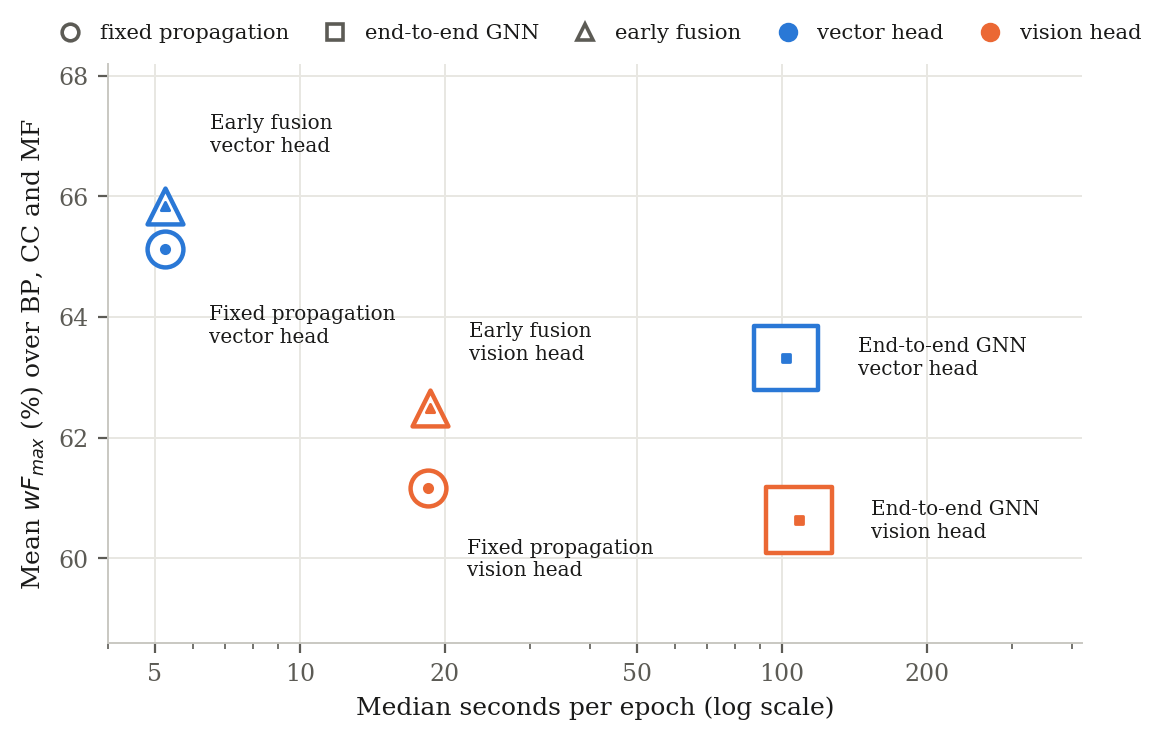
\includegraphics[width=654\px,height=415.4\px]{figures/fig_6_5.png}};
\node[tl] at (88,70) {\fmR\fz{16}{16}\color{inkii}\ls{2}\Ll{5 · Results}};
\node[tl] at (88,131) {\fdA\fz{54}{56.7}\color{ink}\ls{-1}\Ll{A thirteenth of the time per epoch}};
\node<2-5>[tl] at (88,688.4) {\fmR\fz{15}{19.5}\color{muted}\Ll{Dissertation, Fig. 6.5}};
\node<3-5>[tl] at (852,232) {\fbR\fz{26}{35.1}\color{ink}\Ll{Fixed + vector: 5.24 s/epoch, 6.4 GiB peak}};
\node<3-5>[tl] at (852,283.1) {\fbR\fz{26}{35.1}\color{ink}\Ll{GCN alone: 68.76 s/epoch, 14.1 GiB; GAT 161.41 s,\\20.7 GiB}};
\node<4-5>[tl] at (852,369.3) {\fbR\fz{26}{35.1}\color{ink}\Ll{{\fbB{}Matches or beats the GCN at about 1/13 of the time}\\{\fbB{}and under half the memory}}};
\node<5>[tl] at (852,455.5) {\fbR\fz{26}{35.1}\color{ink}\Ll{Early fusion costs the same as fixed propagation once {\fz{29.2}{35}$\mathbf{g}$}\\is stored}};
\node[tr] at (1512,876) {\fmR\fz{16}{16}\color{muted}40 / 45};
\end{tikzpicture}
\note{The fixed operator runs once per experiment; the learned ones recompute a full-graph propagation at every optimization step. 

Early-fusion cost excludes training the GCN checkpoint it consumes.}
\end{frame}

\begin{frame}[plain]
\begin{tikzpicture}[deck]
\node<1>[box] at (0,0) {\includegraphics[page=3,width=1600\px]{build/layers}};
\node<2>[box] at (0,0) {\includegraphics[page=143,width=1600\px]{build/layers}};
\node<3>[box] at (0,0) {\includegraphics[page=144,width=1600\px]{build/layers}};
\node<4>[box] at (0,0) {\includegraphics[page=145,width=1600\px]{build/layers}};
\node<2-4>[box] at (109,235) {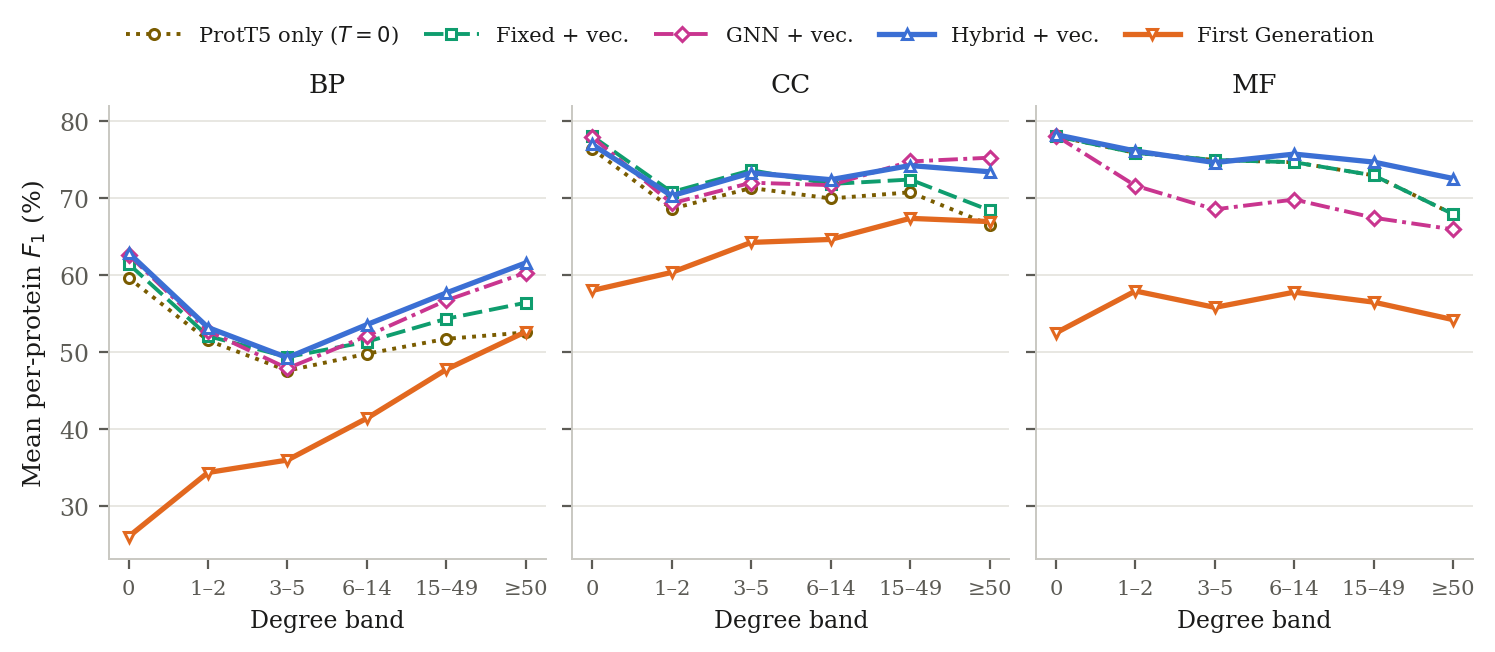
\includegraphics[width=802.5\px,height=350\px]{figures/fig_6_6.png}};
\node[tl] at (88,70) {\fmR\fz{16}{16}\color{inkii}\ls{2}\Ll{5 · Results}};
\node[tl] at (88,131) {\fdA\fz{54}{56.7}\color{ink}\ls{-1}\Ll{The graph helps where there is graph}};
\node<2-4>[tl] at (88,623) {\fmR\fz{15}{19.5}\color{muted}\Ll{Dissertation, Fig. 6.6 · test}};
\node<3-4>[tl] at (1094.7,232) {\fbR\fz{26}{35.1}\color{ink}\Ll{Every ProtT5 route scores worse on\\connected than on isolated proteins}};
\node<3-4>[tl] at (1094.7,318.2) {\fbR\fz{26}{35.1}\color{ink}\Ll{The graph-free control already\\shows it, so the graph does not\\cause it}};
\node<4>[tl] at (1094.7,439.5) {\fbR\fz{26}{35.1}\color{ink}\Ll{The graph's gain grows with degree:\\up to +9.05 BP, +8.71 CC, +4.64 MF\\at degree $\geq$ 50}};
\node[tr] at (1512,876) {\fmR\fz{16}{16}\color{muted}41 / 45};
\end{tikzpicture}
\note{Hubs tend to be multifunctional and harder for a sequence model. In BP the hardest proteins have degree 3 to 5, not zero. 

Degree-zero differences come from rescaling and refitting, so read topological gains from degree one upward.}
\end{frame}

\section{6 · Conclusions}
\begin{frame}[plain]
\begin{tikzpicture}[deck]
\node<1>[box] at (0,0) {\includegraphics[page=3,width=1600\px]{build/layers}};
\node<2>[box] at (0,0) {\includegraphics[page=146,width=1600\px]{build/layers}};
\node<3>[box] at (0,0) {\includegraphics[page=147,width=1600\px]{build/layers}};
\node<4>[box] at (0,0) {\includegraphics[page=148,width=1600\px]{build/layers}};
\node[tl] at (88,70) {\fmR\fz{16}{16}\color{inkii}\ls{2}\Ll{6 · Conclusions}};
\node[tl] at (88,131) {\fdA\fz{54}{56.7}\color{ink}\ls{-1}\Ll{Answers to the research questions}};
\node<2-4>[tc] at (126,232) {\fmM\fz{20}{20}\color{ink}\Lc{RQ1}};
\node<2-4>[tl] at (184,232) {\fbR\fz{20}{26}\color{inkii}\Ll{Which network representation works best?}};
\node<2-4>[tl] at (184,266) {\fbR\fz{27}{35.1}\color{ink}\Ll{The unreduced profile and an MLP; imposed locality hurts}};
\node<2-4>[tc] at (126,321.1) {\fmM\fz{20}{20}\color{ink}\Lc{RQ2}};
\node<2-4>[tl] at (184,321.1) {\fbR\fz{20}{26}\color{inkii}\Ll{How much does propagating ProtT5 over STRING add?}};
\node<2-4>[tl] at (184,355.1) {\fbR\fz{27}{35.1}\color{ink}\Ll{Large gain, mostly from ProtT5; propagation adds +1.87 BP, +2.15 CC, nothing in MF (test)}};
\node<2-4>[tc] at (126,410.2) {\fmM\fz{20}{20}\color{ink}\Lc{RQ3}};
\node<2-4>[tl] at (184,410.2) {\fbR\fz{20}{26}\color{inkii}\Ll{Fixed vs learned aggregation, vector vs image heads}};
\node<2-4>[tl] at (184,444.2) {\fbR\fz{27}{35.1}\color{ink}\Ll{Late 67.06 > Early 65.84 > Fixed 65.12 > GNN 63.32 (validation); vector head throughout}};
\node<3-4>[tc] at (126,499.3) {\fmM\fz{20}{20}\color{ink}\Lc{RQ4}};
\node<3-4>[tl] at (184,499.3) {\fbR\fz{20}{26}\color{inkii}\Ll{Do early and late fusion help?}};
\node<3-4>[tl] at (184,533.3) {\fbR\fz{27}{35.1}\color{ink}\Ll{Both help; late more (+1.26 to +2.18 pp, validation)}};
\node<3-4>[tc] at (126,588.4) {\fmM\fz{20}{20}\color{ink}\Lc{RQ5}};
\node<3-4>[tl] at (184,588.4) {\fbR\fz{20}{26}\color{inkii}\Ll{How deep, and how much retention?}};
\node<3-4>[tl] at (184,622.4) {\fbR\fz{27}{35.1}\color{ink}\Ll{One or two hops, {\fz{30.3}{36.3}$\alpha$} 0.7 to 0.8; MF prefers none}};
\node<4>[tc] at (126,677.5) {\fmM\fz{20}{20}\color{ink}\Lc{RQ6}};
\node<4>[tl] at (184,677.5) {\fbR\fz{20}{26}\color{inkii}\Ll{How does it compare with the literature?}};
\node<4>[tl] at (184,711.5) {\fbR\fz{27}{35.1}\color{ink}\Ll{Best in every column but one; +9.77 / +8.67 / +4.93 pp wF\textsubscript{max} (test)}};
\node<4>[tc] at (126,766.6) {\fmM\fz{20}{20}\color{ink}\Lc{RQ7}};
\node<4>[tl] at (184,766.6) {\fbR\fz{20}{26}\color{inkii}\Ll{Does it work on one global, aggregated network?}};
\node<4>[tl] at (184,800.6) {\fbR\fz{27}{35.1}\color{ink}\Ll{Works on one global aggregated network; partitioned graphs not tested}};
\node[tr] at (1512,876) {\fmR\fz{16}{16}\color{muted}42 / 45};
\end{tikzpicture}
\note{Use the conclusions chapter wording if asked for detail. 

RQ7 is applicability, not superiority over partitioned graphs.}
\end{frame}

\begin{frame}[plain]
\begin{tikzpicture}[deck]
\node<1>[box] at (0,0) {\includegraphics[page=3,width=1600\px]{build/layers}};
\node<2>[box] at (0,0) {\includegraphics[page=149,width=1600\px]{build/layers}};
\node<3>[box] at (0,0) {\includegraphics[page=150,width=1600\px]{build/layers}};
\node<4>[box] at (0,0) {\includegraphics[page=151,width=1600\px]{build/layers}};
\node[tl] at (88,70) {\fmR\fz{16}{16}\color{inkii}\ls{2}\Ll{6 · Conclusions}};
\node[tl] at (88,131) {\fdA\fz{54}{56.7}\color{ink}\ls{-1}\Ll{Limitations}};
\node<2-4>[tl] at (124,236) {\fbR\fz{30}{40.5}\color{ink}\Ll{Single seed; the 0.5 pp floor is a reading convention, not a confidence interval}};
\node<2-4>[tl] at (124,298.5) {\fbR\fz{30}{40.5}\color{ink}\Ll{Random protein-level split: transductive interpolation, possible homology leakage}};
\node<3-4>[tl] at (124,361) {\fbR\fz{30}{40.5}\color{ink}\Ll{STRING scores may encode annotation knowledge (circularity)}};
\node<4>[tl] at (124,423.5) {\fbR\fz{30}{40.5}\color{ink}\Ll{Fixed vs learned is not a single-factor ablation ({\fz{33.7}{40.4}$\alpha^{T}$} scaling, normalization)}};
\node<4>[tl] at (124,486) {\fbR\fz{30}{40.5}\color{ink}\Ll{Baselines adapted to one aggregated network and a reduced label space}};
\node[tr] at (1512,876) {\fmR\fz{16}{16}\color{muted}43 / 45};
\end{tikzpicture}
\note{State these before the committee does. 

Each one is documented in the dissertation with its consequence.}
\end{frame}

\begin{frame}[plain]
\begin{tikzpicture}[deck]
\node<1>[box] at (0,0) {\includegraphics[page=3,width=1600\px]{build/layers}};
\node<2>[box] at (0,0) {\includegraphics[page=152,width=1600\px]{build/layers}};
\node<3>[box] at (0,0) {\includegraphics[page=153,width=1600\px]{build/layers}};
\node[tl] at (88,70) {\fmR\fz{16}{16}\color{inkii}\ls{2}\Ll{6 · Conclusions}};
\node[tl] at (88,131) {\fdA\fz{54}{56.7}\color{ink}\ls{-1}\Ll{Next steps}};
\node<2-3>[tl] at (115,337) {\fbR\fz{27}{35.1}\color{ink}\Ll{Separate the graph by organism,\\or one model per organism}};
\node<2-3>[tl] at (599,337) {\fbR\fz{27}{35.1}\color{ink}\Ll{Keep STRING evidence channels\\apart (typed or parallel edges)}};
\node<2-3>[tl] at (1083,337) {\fbR\fz{27}{35.1}\color{ink}\Ll{Heterogeneous graphs (proteins,\\terms, evidence); compare with\\ProtHGT}};
\node<3>[tl] at (357,604.3) {\fbR\fz{27}{35.1}\color{ink}\Ll{Sampled aggregation\\(GraphSAGE) for a cheaper\\learned route}};
\node<3>[tl] at (841,604.3) {\fbR\fz{27}{35.1}\color{ink}\Ll{Richer node features: structure,\\domains, expression; most\\promising for MF}};
\node[tr] at (1512,876) {\fmR\fz{16}{16}\color{muted}44 / 45};
\end{tikzpicture}
\note{The two most immediate are taxonomic scope and evidence channels. 

MF is where the network contributed least, so new node features matter most there.}
\end{frame}

\begin{frame}[plain]
\begin{tikzpicture}[deck]
\node[box] at (0,0) {\includegraphics[page=154,width=1600\px]{build/layers}};
\node[tl] at (88,367) {\fdB\fz{104}{98.8}\color{ink}\ls{-2.5}\Ll{Thank you}};
\node[tl] at (124,412.8) {\fbR\fz{30}{40.5}\color{ink}\Ll{NEXUS-GO: fixed propagation of ProtT5 over STRING, fused with a GCN, best in every\\ontology at a fraction of the cost}};
\node[tl] at (124,515.8) {\fbR\fz{30}{40.5}\color{ink}\Ll{Code: {\fmR\fz{25.8}{31}{}github.com/ymauhn/nexus-go}}};
\node[tl] at (124,578.3) {\fbR\fz{30}{40.5}\color{ink}\Ll{Publications: VISAPP 2026; extended version accepted in CCIS (expected December 2026)}};
\node[tl] at (124,640.8) {\fbR\fz{30}{40.5}\color{ink}\Ll{Funding: CAPES, BTG Pactual · Computing resources: IC/Unicamp}};
\node[tl] at (88,829) {\fdA\fz{40}{40}\color{ink}\Ll{Questions}};
\end{tikzpicture}
\note{Thank the committee, the advisors and the funders. 

Open for questions.}
\end{frame}

\section{Backup}
\begin{frame}[plain]
\begin{tikzpicture}[deck]
\node[box] at (0,0) {\includegraphics[page=155,width=1600\px]{build/layers}};
\node[tl] at (88,70) {\fmR\fz{16}{16}\color{inkii}\ls{2}\Ll{Backup}};
\node[tl] at (88,131) {\fdA\fz{54}{56.7}\color{ink}\ls{-1}\Ll{Hyperparameters}};
\node[tl] at (100,230) {\fbB\fz{20}{24}\color{inkii}\Ll{Setting}};
\node[tl] at (320.5,230) {\fbB\fz{20}{24}\color{inkii}\Ll{Value}};
\node[tl] at (499,230) {\fbB\fz{20}{24}\color{inkii}\Ll{Scope}};
\node[tl] at (100,264) {\fbR\fz{18}{21.6}\color{ink}\Ll{Optimizer}};
\node[tl] at (320.5,264) {\fbR\fz{18}{21.6}\color{ink}\Ll{Adam}};
\node[tl] at (499,264) {\fbR\fz{18}{21.6}\color{ink}\Ll{all families}};
\node[tl] at (100,299) {\fbR\fz{18}{21.6}\color{ink}\Ll{Learning rate}};
\node[tl] at (320.5,299) {\fbR\fz{18}{21.6}\color{ink}\Ll{1 × 10\textsuperscript{-4}}};
\node[tl] at (499,299) {\fbR\fz{18}{21.6}\color{ink}\Ll{all families}};
\node[tl] at (100,334) {\fbR\fz{18}{21.6}\color{ink}\Ll{Weight decay}};
\node[tl] at (320.5,334) {\fbR\fz{18}{21.6}\color{ink}\Ll{none}};
\node[tl] at (499,334) {\fbR\fz{18}{21.6}\color{ink}\Ll{all families}};
\node[tl] at (100,369) {\fbR\fz{18}{21.6}\color{ink}\Ll{Learning-rate schedule}};
\node[tl] at (320.5,369) {\fbR\fz{18}{21.6}\color{ink}\Ll{none}};
\node[tl] at (499,369) {\fbR\fz{18}{21.6}\color{ink}\Ll{all families}};
\node[tl] at (100,404) {\fbR\fz{18}{21.6}\color{ink}\Ll{Batch size}};
\node[tl] at (320.5,404) {\fbR\fz{18}{21.6}\color{ink}\Ll{256}};
\node[tl] at (499,404) {\fbR\fz{18}{21.6}\color{ink}\Ll{all families}};
\node[tl] at (100,439) {\fbR\fz{18}{21.6}\color{ink}\Ll{Maximum epochs}};
\node[tl] at (320.5,439) {\fbR\fz{18}{21.6}\color{ink}\Ll{250}};
\node[tl] at (499,439) {\fbR\fz{18}{21.6}\color{ink}\Ll{all families}};
\node[tl] at (100,474) {\fbR\fz{18}{21.6}\color{ink}\Ll{Early-stopping patience}};
\node[tl] at (320.5,474) {\fbR\fz{18}{21.6}\color{ink}\Ll{20 epochs}};
\node[tl] at (499,474) {\fbR\fz{18}{21.6}\color{ink}\Ll{all families}};
\node[tl] at (100,509) {\fbR\fz{18}{21.6}\color{ink}\Ll{Monitored quantity}};
\node[tl] at (320.5,509) {\fbR\fz{18}{21.6}\color{ink}\Ll{validation loss}};
\node[tl] at (499,509) {\fbR\fz{18}{21.6}\color{ink}\Ll{all families}};
\node[tl] at (100,544) {\fbR\fz{18}{21.6}\color{ink}\Ll{Minimum improvement}};
\node[tl] at (320.5,544) {\fbR\fz{18}{21.6}\color{ink}\Ll{0}};
\node[tl] at (499,544) {\fbR\fz{18}{21.6}\color{ink}\Ll{all families}};
\node[tl] at (100,579) {\fbR\fz{18}{21.6}\color{ink}\Ll{Objective}};
\node[tl] at (320.5,579) {\fbR\fz{18}{21.6}\color{ink}\Ll{Eq. 5.20}};
\node[tl] at (499,579) {\fbR\fz{18}{21.6}\color{ink}\Ll{all families}};
\node[tl] at (100,614) {\fbR\fz{18}{21.6}\color{ink}\Ll{Class weighting}};
\node[tl] at (320.5,614) {\fbR\fz{18}{21.6}\color{ink}\Ll{information content}};
\node[tl] at (499,614) {\fbR\fz{18}{21.6}\color{ink}\Ll{all families}};
\node[tl] at (100,649) {\fbR\fz{18}{21.6}\color{ink}\Ll{Dropout, prediction head}};
\node[tl] at (320.5,649) {\fbR\fz{18}{21.6}\color{ink}\Ll{0.4}};
\node[tl] at (499,649) {\fbR\fz{18}{21.6}\color{ink}\Ll{all families}};
\node[tl] at (88,686) {\fmR\fz{15}{19.5}\color{muted}\Ll{Dissertation, Table A.2}};
\node[tl] at (828,230) {\fbB\fz{20}{24}\color{inkii}\Ll{Setting}};
\node[tl] at (1072.2,230) {\fbB\fz{20}{24}\color{inkii}\Ll{Value}};
\node[tl] at (1359,230) {\fbB\fz{20}{24}\color{inkii}\Ll{Scope}};
\node[tl] at (828,264) {\fbR\fz{18}{24}\color{ink}\Ll{Dropout, between\\convolutions}};
\node[tl] at (1072.2,264) {\fbR\fz{18}{21.6}\color{ink}\Ll{0.3}};
\node[tl] at (1359,264) {\fbR\fz{18}{24}\color{ink}\Ll{graph\\convolutions}};
\node[tl] at (828,323) {\fbR\fz{18}{21.6}\color{ink}\Ll{Hidden widths, head}};
\node[tl] at (1072.2,323) {\fbR\fz{18}{21.6}\color{ink}\Ll{[1024, 512]}};
\node[tl] at (1359,323) {\fbR\fz{18}{21.6}\color{ink}\Ll{all families}};
\node[tl] at (828,358) {\fbR\fz{18}{21.6}\color{ink}\Ll{Convolution hidden width}};
\node[tl] at (1072.2,358) {\fbR\fz{18}{21.6}\color{ink}\Ll{1024}};
\node[tl] at (1359,358) {\fbR\fz{18}{24}\color{ink}\Ll{graph\\convolutions}};
\node[tl] at (828,417) {\fbR\fz{18}{21.6}\color{ink}\Ll{Convolution layers}};
\node[tl] at (1072.2,417) {\fbR\fz{18}{21.6}\color{ink}\Ll{2}};
\node[tl] at (1359,417) {\fbR\fz{18}{24}\color{ink}\Ll{graph\\convolutions}};
\node[tl] at (828,476) {\fbR\fz{18}{21.6}\color{ink}\Ll{Attention heads}};
\node[tl] at (1072.2,476) {\fbR\fz{18}{21.6}\color{ink}\Ll{4 (hidden), 1 (output)}};
\node[tl] at (1359,476) {\fbR\fz{18}{21.6}\color{ink}\Ll{graph attention}};
\node[tl] at (828,511) {\fbR\fz{18}{21.6}\color{ink}\Ll{Random seed}};
\node[tl] at (1072.2,511) {\fbR\fz{18}{21.6}\color{ink}\Ll{1337}};
\node[tl] at (1359,511) {\fbR\fz{18}{21.6}\color{ink}\Ll{all families}};
\node[tl] at (828,546) {\fbR\fz{18}{21.6}\color{ink}\Ll{Data-loading workers}};
\node[tl] at (1072.2,546) {\fbR\fz{18}{21.6}\color{ink}\Ll{4}};
\node[tl] at (1359,546) {\fbR\fz{18}{21.6}\color{ink}\Ll{all families}};
\node[tl] at (828,581) {\fbR\fz{18}{21.6}\color{ink}\Ll{Configured edge threshold}};
\node[tl] at (1072.2,581) {\fbR\fz{18}{24}\color{ink}\Ll{0.10 (inert; source-data floor =\\0.400)}};
\node[tl] at (1359,581) {\fbR\fz{18}{21.6}\color{ink}\Ll{all families}};
\node[tl] at (828,640) {\fbR\fz{18}{21.6}\color{ink}\Ll{Propagation steps T}};
\node[tl] at (1072.2,640) {\fbR\fz{18}{21.6}\color{ink}\Ll{varies}};
\node[tl] at (1359,640) {\fbR\fz{18}{21.6}\color{ink}\Ll{fixed propagation}};
\node[tl] at (828,676) {\fbR\fz{18}{21.6}\color{ink}\Ll{Mixing coefficient $\alpha$}};
\node[tl] at (1072.2,675) {\fbR\fz{18}{21.6}\color{ink}\Ll{varies}};
\node[tl] at (1359,675) {\fbR\fz{18}{21.6}\color{ink}\Ll{fixed propagation}};
\node[tl] at (828,711) {\fbR\fz{18}{21.6}\color{ink}\Ll{Deduplication rule}};
\node[tl] at (1072.2,711) {\fbR\fz{18}{21.6}\color{ink}\Ll{varies}};
\node[tl] at (1359,711) {\fbR\fz{18}{21.6}\color{ink}\Ll{all families}};
\node[tl] at (816,748) {\fmR\fz{15}{19.5}\color{muted}\Ll{Dissertation, Table A.2}};
\node[tr] at (1512,876) {\fmR\fz{16}{16}\color{muted}B1};
\end{tikzpicture}
\note{Optimization settings of the final second-generation campaign (Table A.2). Values marked varies are part of the search space.}
\end{frame}

\begin{frame}[plain]
\begin{tikzpicture}[deck]
\node[box] at (0,0) {\includegraphics[page=156,width=1600\px]{build/layers}};
\node[tl] at (88,70) {\fmR\fz{16}{16}\color{inkii}\ls{2}\Ll{Backup}};
\node[tl] at (88,131) {\fdA\fz{54}{56.7}\color{ink}\ls{-1}\Ll{Late fusion: grid and selected coefficients}};
\node[tl] at (100,230) {\fbB\fz{20}{24}\color{inkii}\Ll{Rule}};
\node[tl] at (381.2,230) {\fbB\fz{20}{24}\color{inkii}\Ll{Grid}};
\node[tl] at (826.4,230) {\fbB\fz{20}{24}\color{inkii}\Ll{Config.}};
\node[tl] at (100,264) {\fbR\fz{18}{21.6}\color{ink}\Ll{Linear combination}};
\node[tl] at (381.2,265) {\fbR\fz{18}{21.6}\color{ink}\Ll{$\gamma$ from 0.00 to 1.00 in steps of 0.05}};
\node[tl] at (826.4,264) {\fbR\fz{18}{21.6}\color{ink}\Ll{21}};
\node[tl] at (100,300) {\fbR\fz{18}{24}\color{ink}\Ll{Pointwise maximum and\\minimum}};
\node[tl] at (381.2,300) {\fbR\fz{18}{21.6}\color{ink}\Ll{no parameter}};
\node[tl] at (826.4,300) {\fbR\fz{18}{21.6}\color{ink}\Ll{2}};
\node[tl] at (100,359) {\fbR\fz{18}{21.6}\color{ink}\Ll{Term-specific weighting}};
\node[tl] at (381.2,360) {\fbR\fz{18}{21.6}\color{ink}\Ll{IC\textsubscript{thr} $\in$ \{0.4, 1.1, 2.1, 3.4\} and $\kappa$\textsubscript{IC} $\in$ \{1, 2, 5\}}};
\node[tl] at (826.4,359) {\fbR\fz{18}{21.6}\color{ink}\Ll{12}};
\node[tl] at (100,395) {\fbR\fz{18}{21.6}\color{ink}\Ll{Protein-specific weighting}};
\node[tl] at (381.2,396) {\fbR\fz{18}{24}\color{ink}\Ll{d\textsubscript{thr} $\in$ \{1, 3, 5, 14, 28\} and $\kappa$\textsubscript{deg} $\in$ \{0.25, 0.50, 0.75,\\1.00\}}};
\node[tl] at (826.4,395) {\fbR\fz{18}{21.6}\color{ink}\Ll{20}};
\node[tl] at (100,455) {\fbR\fz{18}{21.6}\color{ink}\Ll{Combined weighting}};
\node[tl] at (381.2,456) {\fbR\fz{18}{21.6}\color{ink}\Ll{$\lambda$ from 0.0 to 1.0 in steps of 0.1}};
\node[tl] at (826.4,455) {\fbR\fz{18}{21.6}\color{ink}\Ll{11}};
\node[tl] at (100,491) {\fbR\fz{18}{21.6}\color{ink}\Ll{Stacking}};
\node[tl] at (381.2,491) {\fbR\fz{18}{21.6}\color{ink}\Ll{five meta-classifiers, no coefficient swept}};
\node[tl] at (826.4,491) {\fbR\fz{18}{21.6}\color{ink}\Ll{5}};
\node[tl] at (100,526) {\fbR\fz{18}{21.6}\color{ink}\Ll{Total}};
\node[tl] at (826.4,526) {\fbR\fz{18}{21.6}\color{ink}\Ll{71}};
\node[tl] at (88,563) {\fmR\fz{15}{19.5}\color{muted}\Ll{Dissertation, Table A.3}};
\node[tl] at (949.3,230) {\fbB\fz{20}{24}\color{inkii}\Ll{Rule}};
\node[tr] at (1281.6,230) {\fbB\fz{20}{24}\color{inkii}\Lr{Coefficient}};
\node[tr] at (1348.8,230) {\fbB\fz{20}{24}\color{inkii}\Lr{BP}};
\node[tr] at (1416,230) {\fbB\fz{20}{24}\color{inkii}\Lr{CC}};
\node[tr] at (1483.2,230) {\fbB\fz{20}{24}\color{inkii}\Lr{MF}};
\node[tl] at (949.3,264) {\fbR\fz{18}{21.6}\color{ink}\Ll{Linear combination}};
\node[tr] at (1281.6,264.5) {\fmR\fz{18}{21.6}\color{ink}\Lr{$\gamma$}};
\node[tr] at (1348.8,264.5) {\fmR\fz{18}{21.6}\color{ink}\Lr{0.50}};
\node[tr] at (1416,264.5) {\fmR\fz{18}{21.6}\color{ink}\Lr{0.55}};
\node[tr] at (1483.2,264.5) {\fmR\fz{18}{21.6}\color{ink}\Lr{0.55}};
\node[tl] at (949.3,299) {\fbR\fz{18}{21.6}\color{ink}\Ll{Term-specific weighting}};
\node[tr] at (1281.6,299.5) {\fmR\fz{18}{21.6}\color{ink}\Lr{IC\textsubscript{thr}}};
\node[tr] at (1348.8,299.5) {\fmR\fz{18}{21.6}\color{ink}\Lr{1.1}};
\node[tr] at (1416,299.5) {\fmR\fz{18}{21.6}\color{ink}\Lr{0.4}};
\node[tr] at (1483.2,299.5) {\fmR\fz{18}{21.6}\color{ink}\Lr{0.4}};
\node[tr] at (1281.6,334) {\fmR\fz{18}{21.6}\color{ink}\Lr{$\kappa$\textsubscript{IC}}};
\node[tr] at (1348.8,334) {\fmR\fz{18}{21.6}\color{ink}\Lr{1.0}};
\node[tr] at (1416,334) {\fmR\fz{18}{21.6}\color{ink}\Lr{1.0}};
\node[tr] at (1483.2,334) {\fmR\fz{18}{21.6}\color{ink}\Lr{1.0}};
\node[tl] at (949.3,368) {\fbR\fz{18}{21.6}\color{ink}\Ll{Protein-specific weighting}};
\node[tr] at (1281.6,368.5) {\fmR\fz{18}{21.6}\color{ink}\Lr{d\textsubscript{thr}}};
\node[tr] at (1348.8,368.5) {\fmR\fz{18}{21.6}\color{ink}\Lr{3}};
\node[tr] at (1416,368.5) {\fmR\fz{18}{21.6}\color{ink}\Lr{14}};
\node[tr] at (1483.2,368.5) {\fmR\fz{18}{21.6}\color{ink}\Lr{28}};
\node[tr] at (1281.6,403) {\fmR\fz{18}{21.6}\color{ink}\Lr{$\kappa$\textsubscript{deg}}};
\node[tr] at (1348.8,403) {\fmR\fz{18}{21.6}\color{ink}\Lr{0.25}};
\node[tr] at (1416,403) {\fmR\fz{18}{21.6}\color{ink}\Lr{0.25}};
\node[tr] at (1483.2,403) {\fmR\fz{18}{21.6}\color{ink}\Lr{0.25}};
\node[tl] at (949.3,437) {\fbR\fz{18}{21.6}\color{ink}\Ll{Combined weighting}};
\node[tr] at (1281.6,437.5) {\fmR\fz{18}{21.6}\color{ink}\Lr{$\lambda$}};
\node[tr] at (1348.8,437.5) {\fmR\fz{18}{21.6}\color{ink}\Lr{0.5}};
\node[tr] at (1416,437.5) {\fmR\fz{18}{21.6}\color{ink}\Lr{0.4}};
\node[tr] at (1483.2,437.5) {\fmR\fz{18}{21.6}\color{ink}\Lr{0.9}};
\node[tl] at (937.3,474) {\fmR\fz{15}{19.5}\color{muted}\Ll{Dissertation, Table A.4}};
\node[tr] at (1512,876) {\fmR\fz{16}{16}\color{muted}B2};
\end{tikzpicture}
\note{71 configurations per ontology, chosen on validation. Both conditional rules converged on the flattest sigmoid the grid offers.}
\end{frame}

\begin{frame}[plain]
\begin{tikzpicture}[deck]
\node[box] at (0,0) {\includegraphics[page=157,width=1600\px]{build/layers}};
\node[tl] at (88,70) {\fmR\fz{16}{16}\color{inkii}\ls{2}\Ll{Backup}};
\node[tl] at (88,131) {\fdA\fz{54}{56.7}\color{ink}\ls{-1}\Ll{Early fusion: provenance × source}};
\node[tl] at (100,230) {\fbB\fz{20}{24}\color{inkii}\Ll{Head}};
\node[tr] at (239.5,230) {\fbB\fz{20}{24}\color{inkii}\Lr{Fusion}};
\node[tr] at (371,230) {\fbB\fz{20}{24}\color{inkii}\Lr{Provenance}};
\node[tr] at (459.8,230) {\fbB\fz{20}{24}\color{inkii}\Lr{Source}};
\node[tr] at (537.8,230) {\fbB\fz{20}{24}\color{inkii}\Lr{BP}};
\node[tr] at (615.8,230) {\fbB\fz{20}{24}\color{inkii}\Lr{CC}};
\node[tr] at (693.8,230) {\fbB\fz{20}{24}\color{inkii}\Lr{MF}};
\node[tl] at (100,264) {\fbR\fz{18}{21.6}\color{ink}\Ll{Vector}};
\node[tr] at (239.5,264.5) {\fmR\fz{18}{21.6}\color{ink}\Lr{add}};
\node[tr] at (371,264.5) {\fmR\fz{18}{21.6}\color{ink}\Lr{vector}};
\node[tr] at (459.8,264.5) {\fmR\fz{18}{21.6}\color{ink}\Lr{vector}};
\node[tr] at (537.8,264.5) {\fmR\fz{18}{21.6}\color{ink}\Lr{56.52}};
\node[tr] at (615.8,264.5) {\fmR\fz{18}{21.6}\color{ink}\Lr{66.86}};
\node[tr] at (693.8,264.5) {\fmR\fz{18}{21.6}\color{ink}\Lr{73.81}};
\node[tr] at (239.5,299) {\fmR\fz{18}{21.6}\color{ink}\Lr{add}};
\node[tr] at (371,299) {\fmR\fz{18}{21.6}\color{ink}\Lr{vector}};
\node[tr] at (459.8,299) {\fmR\fz{18}{21.6}\color{ink}\Lr{vision}};
\node[tr] at (537.8,299) {\fmR\fz{18}{21.6}\color{ink}\Lr{55.73}};
\node[tr] at (615.8,299) {\fmR\fz{18}{21.6}\color{ink}\Lr{65.79}};
\node[tr] at (693.8,299) {\fmR\fz{18}{21.6}\color{ink}\Lr{n/a}};
\node[tr] at (239.5,333) {\fmR\fz{18}{21.6}\color{ink}\Lr{add}};
\node[tr] at (371,333) {\fmR\fz{18}{21.6}\color{ink}\Lr{vision}};
\node[tr] at (459.8,333) {\fmR\fz{18}{21.6}\color{ink}\Lr{vector}};
\node[tr] at (537.8,333) {\fmR\fz{18}{21.6}\color{ink}\Lr{53.98}};
\node[tr] at (615.8,333) {\fmR\fz{18}{21.6}\color{ink}\Lr{67.07}};
\node[tr] at (693.8,333) {\fmR\fz{18}{21.6}\color{ink}\Lr{73.42}};
\node[tr] at (239.5,367) {\fmR\fz{18}{21.6}\color{ink}\Lr{add}};
\node[tr] at (371,367) {\fmR\fz{18}{21.6}\color{ink}\Lr{vision}};
\node[tr] at (459.8,367) {\fmR\fz{18}{21.6}\color{ink}\Lr{vision}};
\node[tr] at (537.8,367) {\fmR\fz{18}{21.6}\color{ink}\Lr{52.96}};
\node[tr] at (615.8,367) {\fmR\fz{18}{21.6}\color{ink}\Lr{65.46}};
\node[tr] at (693.8,367) {\fmR\fz{18}{21.6}\color{ink}\Lr{n/a}};
\node[tr] at (239.5,401) {\fmR\fz{18}{21.6}\color{ink}\Lr{concat}};
\node[tr] at (371,401) {\fmR\fz{18}{21.6}\color{ink}\Lr{vector}};
\node[tr] at (459.8,401) {\fmR\fz{18}{21.6}\color{ink}\Lr{vector}};
\node[tr] at (537.8,401) {\fmR\fz{18}{21.6}\color{ink}\Lr{56.05}};
\node[tr] at (615.8,401) {\fmR\fz{18}{21.6}\color{ink}\Lr{67.12}};
\node[tr] at (693.8,401) {\fmR\fz{18}{21.6}\color{ink}\Lr{73.68}};
\node[tr] at (239.5,435) {\fmR\fz{18}{21.6}\color{ink}\Lr{concat}};
\node[tr] at (371,435) {\fmR\fz{18}{21.6}\color{ink}\Lr{vector}};
\node[tr] at (459.8,435) {\fmR\fz{18}{21.6}\color{ink}\Lr{vision}};
\node[tr] at (537.8,435) {\fmR\fz{18}{21.6}\color{ink}\Lr{55.52}};
\node[tr] at (615.8,435) {\fmR\fz{18}{21.6}\color{ink}\Lr{65.27}};
\node[tr] at (693.8,435) {\fmR\fz{18}{21.6}\color{ink}\Lr{n/a}};
\node[tr] at (239.5,469) {\fmR\fz{18}{21.6}\color{ink}\Lr{concat}};
\node[tr] at (371,469) {\fmR\fz{18}{21.6}\color{ink}\Lr{vision}};
\node[tr] at (459.8,469) {\fmR\fz{18}{21.6}\color{ink}\Lr{vector}};
\node[tr] at (537.8,469) {\fmR\fz{18}{21.6}\color{ink}\Lr{55.32}};
\node[tr] at (615.8,469) {\fmR\fz{18}{21.6}\color{ink}\Lr{67.20}};
\node[tr] at (693.8,469) {\fmR\fz{18}{21.6}\color{ink}\Lr{73.78}};
\node[tr] at (239.5,503) {\fmR\fz{18}{21.6}\color{ink}\Lr{concat}};
\node[tr] at (371,503) {\fmR\fz{18}{21.6}\color{ink}\Lr{vision}};
\node[tr] at (459.8,503) {\fmR\fz{18}{21.6}\color{ink}\Lr{vision}};
\node[tr] at (537.8,503) {\fmR\fz{18}{21.6}\color{ink}\Lr{53.23}};
\node[tr] at (615.8,503) {\fmR\fz{18}{21.6}\color{ink}\Lr{65.42}};
\node[tr] at (693.8,503) {\fmR\fz{18}{21.6}\color{ink}\Lr{n/a}};
\node[tl] at (100,537) {\fbR\fz{18}{21.6}\color{ink}\Ll{Vision}};
\node[tr] at (239.5,537.5) {\fmR\fz{18}{21.6}\color{ink}\Lr{add}};
\node[tr] at (371,537.5) {\fmR\fz{18}{21.6}\color{ink}\Lr{vector}};
\node[tr] at (459.8,537.5) {\fmR\fz{18}{21.6}\color{ink}\Lr{vector}};
\node[tr] at (537.8,537.5) {\fmR\fz{18}{21.6}\color{ink}\Lr{52.36}};
\node[tr] at (615.8,537.5) {\fmR\fz{18}{21.6}\color{ink}\Lr{64.77}};
\node[tr] at (693.8,537.5) {\fmR\fz{18}{21.6}\color{ink}\Lr{69.52}};
\node[tr] at (239.5,572) {\fmR\fz{18}{21.6}\color{ink}\Lr{add}};
\node[tr] at (371,572) {\fmR\fz{18}{21.6}\color{ink}\Lr{vector}};
\node[tr] at (459.8,572) {\fmR\fz{18}{21.6}\color{ink}\Lr{vision}};
\node[tr] at (537.8,572) {\fmR\fz{18}{21.6}\color{ink}\Lr{53.17}};
\node[tr] at (615.8,572) {\fmR\fz{18}{21.6}\color{ink}\Lr{64.71}};
\node[tr] at (693.8,572) {\fmR\fz{18}{21.6}\color{ink}\Lr{n/a}};
\node[tr] at (239.5,606) {\fmR\fz{18}{21.6}\color{ink}\Lr{add}};
\node[tr] at (371,606) {\fmR\fz{18}{21.6}\color{ink}\Lr{vision}};
\node[tr] at (459.8,606) {\fmR\fz{18}{21.6}\color{ink}\Lr{vector}};
\node[tr] at (537.8,606) {\fmR\fz{18}{21.6}\color{ink}\Lr{49.72}};
\node[tr] at (615.8,606) {\fmR\fz{18}{21.6}\color{ink}\Lr{62.66}};
\node[tr] at (693.8,606) {\fmR\fz{18}{21.6}\color{ink}\Lr{67.66}};
\node[tr] at (239.5,640) {\fmR\fz{18}{21.6}\color{ink}\Lr{add}};
\node[tr] at (371,640) {\fmR\fz{18}{21.6}\color{ink}\Lr{vision}};
\node[tr] at (459.8,640) {\fmR\fz{18}{21.6}\color{ink}\Lr{vision}};
\node[tr] at (537.8,640) {\fmR\fz{18}{21.6}\color{ink}\Lr{50.21}};
\node[tr] at (615.8,640) {\fmR\fz{18}{21.6}\color{ink}\Lr{62.64}};
\node[tr] at (693.8,640) {\fmR\fz{18}{21.6}\color{ink}\Lr{n/a}};
\node[tl] at (88,676) {\fmR\fz{15}{19.5}\color{muted}\Ll{Dissertation, Table 6.13}};
\node[tr] at (1512,876) {\fmR\fz{16}{16}\color{muted}B3};
\end{tikzpicture}
\note{Provenance is the head with which the consumed GNN embedding was trained; source is the head whose depth and retention were used for the fixed branch. Validation set.}
\end{frame}

\begin{frame}[plain]
\begin{tikzpicture}[deck]
\node[box] at (0,0) {\includegraphics[page=158,width=1600\px]{build/layers}};
\node[tl] at (88,70) {\fmR\fz{16}{16}\color{inkii}\ls{2}\Ll{Backup}};
\node[tl] at (88,131) {\fdA\fz{54}{56.7}\color{ink}\ls{-1}\Ll{Isolated vs connected proteins}};
\node[tl] at (100,230) {\fbB\fz{20}{24}\color{inkii}\Ll{Route}};
\node[tr] at (601.1,230) {\fbB\fz{20}{24}\color{inkii}\Lr{BP}};
\node[tr] at (845.9,230) {\fbB\fz{20}{24}\color{inkii}\Lr{CC}};
\node[tr] at (1090.7,230) {\fbB\fz{20}{24}\color{inkii}\Lr{MF}};
\node[tr] at (434.3,265) {\fbB\fz{20}{24}\color{inkii}\Lr{Isol.}};
\node[tr] at (512.3,265) {\fbB\fz{20}{24}\color{inkii}\Lr{Conn.}};
\node[tr] at (601.1,265) {\fbB\fz{20}{24}\color{inkii}\Lr{$\Delta$}};
\node[tr] at (679.1,265) {\fbB\fz{20}{24}\color{inkii}\Lr{Isol.}};
\node[tr] at (757.1,265) {\fbB\fz{20}{24}\color{inkii}\Lr{Conn.}};
\node[tr] at (845.9,265) {\fbB\fz{20}{24}\color{inkii}\Lr{$\Delta$}};
\node[tr] at (923.9,265) {\fbB\fz{20}{24}\color{inkii}\Lr{Isol.}};
\node[tr] at (1001.9,265) {\fbB\fz{20}{24}\color{inkii}\Lr{Conn.}};
\node[tr] at (1090.7,265) {\fbB\fz{20}{24}\color{inkii}\Lr{$\Delta$}};
\node[tl] at (100,299) {\fbR\fz{18}{21.6}\color{ink}\Ll{ProtT5 only (T=0)}};
\node[tr] at (434.3,299.5) {\fmR\fz{18}{21.6}\color{ink}\Lr{59.89}};
\node[tr] at (512.3,299.5) {\fmR\fz{18}{21.6}\color{ink}\Lr{50.23}};
\node[tr] at (601.1,299.5) {\fmR\fz{18}{21.6}\color{ink}\Lr{−9.66}};
\node[tr] at (679.1,299.5) {\fmR\fz{18}{21.6}\color{ink}\Lr{69.30}};
\node[tr] at (757.1,299.5) {\fmR\fz{18}{21.6}\color{ink}\Lr{62.38}};
\node[tr] at (845.9,299.5) {\fmR\fz{18}{21.6}\color{ink}\Lr{−6.92}};
\node[tr] at (923.9,299.5) {\fmR\fz{18}{21.6}\color{ink}\Lr{75.68}};
\node[tr] at (1001.9,299.5) {\fmR\fz{18}{21.6}\color{ink}\Lr{71.23}};
\node[tr] at (1090.7,299.5) {\fmR\fz{18}{21.6}\color{ink}\Lr{−4.45}};
\node[tl] at (100,334) {\fbR\fz{18}{21.6}\color{ink}\Ll{Fixed propagation + vector head}};
\node[tr] at (434.3,334.5) {\fmR\fz{18}{21.6}\color{ink}\Lr{61.30}};
\node[tr] at (512.3,334.5) {\fmR\fz{18}{21.6}\color{ink}\Lr{52.39}};
\node[tr] at (601.1,334.5) {\fmR\fz{18}{21.6}\color{ink}\Lr{−8.91}};
\node[tr] at (679.1,334.5) {\fmR\fz{18}{21.6}\color{ink}\Lr{71.12}};
\node[tr] at (757.1,334.5) {\fmR\fz{18}{21.6}\color{ink}\Lr{64.77}};
\node[tr] at (845.9,334.5) {\fmR\fz{18}{21.6}\color{ink}\Lr{−6.35}};
\node[tr] at (923.9,334.5) {\fmR\fz{18}{21.6}\color{ink}\Lr{75.68}};
\node[tr] at (1001.9,334.5) {\fmR\fz{18}{21.6}\color{ink}\Lr{71.23}};
\node[tr] at (1090.7,334.5) {\fmR\fz{18}{21.6}\color{ink}\Lr{−4.45}};
\node[tl] at (100,369) {\fbR\fz{18}{21.6}\color{ink}\Ll{End-to-end GNN + vector head}};
\node[tr] at (434.3,369.5) {\fmR\fz{18}{21.6}\color{ink}\Lr{62.26}};
\node[tr] at (512.3,369.5) {\fmR\fz{18}{21.6}\color{ink}\Lr{53.97}};
\node[tr] at (601.1,369.5) {\fmR\fz{18}{21.6}\color{ink}\Lr{−8.29}};
\node[tr] at (679.1,369.5) {\fmR\fz{18}{21.6}\color{ink}\Lr{70.44}};
\node[tr] at (757.1,369.5) {\fmR\fz{18}{21.6}\color{ink}\Lr{64.76}};
\node[tr] at (845.9,369.5) {\fmR\fz{18}{21.6}\color{ink}\Lr{−5.68}};
\node[tr] at (923.9,369.5) {\fmR\fz{18}{21.6}\color{ink}\Lr{74.99}};
\node[tr] at (1001.9,369.5) {\fmR\fz{18}{21.6}\color{ink}\Lr{64.30}};
\node[tr] at (1090.7,369.5) {\fmR\fz{18}{21.6}\color{ink}\Lr{−10.69}};
\node[tl] at (100,404) {\fbR\fz{18}{21.6}\color{ink}\Ll{Early fusion + vector head}};
\node[tr] at (434.3,404.5) {\fmR\fz{18}{21.6}\color{ink}\Lr{62.46}};
\node[tr] at (512.3,404.5) {\fmR\fz{18}{21.6}\color{ink}\Lr{54.58}};
\node[tr] at (601.1,404.5) {\fmR\fz{18}{21.6}\color{ink}\Lr{−7.88}};
\node[tr] at (679.1,404.5) {\fmR\fz{18}{21.6}\color{ink}\Lr{69.41}};
\node[tr] at (757.1,404.5) {\fmR\fz{18}{21.6}\color{ink}\Lr{66.08}};
\node[tr] at (845.9,404.5) {\fmR\fz{18}{21.6}\color{ink}\Lr{−3.33}};
\node[tr] at (923.9,404.5) {\fmR\fz{18}{21.6}\color{ink}\Lr{74.85}};
\node[tr] at (1001.9,404.5) {\fmR\fz{18}{21.6}\color{ink}\Lr{72.05}};
\node[tr] at (1090.7,404.5) {\fmR\fz{18}{21.6}\color{ink}\Lr{−2.80}};
\node[tl] at (100,439) {\fbR\fz{18}{21.6}\color{ink}\Ll{First Generation}};
\node[tr] at (434.3,439.5) {\fmR\fz{18}{21.6}\color{ink}\Lr{24.86}};
\node[tr] at (512.3,439.5) {\fmR\fz{18}{21.6}\color{ink}\Lr{43.88}};
\node[tr] at (601.1,439.5) {\fmR\fz{18}{21.6}\color{ink}\Lr{+19.02}};
\node[tr] at (679.1,439.5) {\fmR\fz{18}{21.6}\color{ink}\Lr{33.97}};
\node[tr] at (757.1,439.5) {\fmR\fz{18}{21.6}\color{ink}\Lr{53.74}};
\node[tr] at (845.9,439.5) {\fmR\fz{18}{21.6}\color{ink}\Lr{+19.77}};
\node[tr] at (923.9,439.5) {\fmR\fz{18}{21.6}\color{ink}\Lr{35.68}};
\node[tr] at (1001.9,439.5) {\fmR\fz{18}{21.6}\color{ink}\Lr{51.95}};
\node[tr] at (1090.7,439.5) {\fmR\fz{18}{21.6}\color{ink}\Lr{+16.27}};
\node[tl] at (88,476) {\fmR\fz{15}{19.5}\color{muted}\Ll{Dissertation, Table 6.22}};
\node[tr] at (1512,876) {\fmR\fz{16}{16}\color{muted}B4};
\end{tikzpicture}
\note{wF\textsubscript{max} on the test set. Every ProtT5 route scores worse on connected proteins; the First Generation is the only route that improves with connectivity.}
\end{frame}

\begin{frame}[plain]
\begin{tikzpicture}[deck]
\node[box] at (0,0) {\includegraphics[page=159,width=1600\px]{build/layers}};
\node[tl] at (88,70) {\fmR\fz{16}{16}\color{inkii}\ls{2}\Ll{Backup}};
\node[tl] at (88,131) {\fdA\fz{54}{56.7}\color{ink}\ls{-1}\Ll{Degree and per-protein F\textsubscript{{\ls{-1.5}{}1}}}};
\node[tl] at (100,230) {\fbB\fz{20}{24}\color{inkii}\Ll{Route}};
\node[tr] at (590.3,230) {\fbB\fz{20}{24}\color{inkii}\Lr{BP}};
\node[tr] at (824.3,230) {\fbB\fz{20}{24}\color{inkii}\Lr{CC}};
\node[tr] at (1058.3,230) {\fbB\fz{20}{24}\color{inkii}\Lr{MF}};
\node[tr] at (423.5,265) {\fbB\fz{20}{24}\color{inkii}\Lr{$\tau$}};
\node[tr] at (512.3,265) {\fbB\fz{20}{24}\color{inkii}\Lr{$\rho$}};
\node[tr] at (590.3,265) {\fbB\fz{20}{24}\color{inkii}\Lr{F\textsubscript{1}}};
\node[tr] at (657.5,265) {\fbB\fz{20}{24}\color{inkii}\Lr{$\tau$}};
\node[tr] at (746.3,265) {\fbB\fz{20}{24}\color{inkii}\Lr{$\rho$}};
\node[tr] at (824.3,265) {\fbB\fz{20}{24}\color{inkii}\Lr{F\textsubscript{1}}};
\node[tr] at (891.5,265) {\fbB\fz{20}{24}\color{inkii}\Lr{$\tau$}};
\node[tr] at (980.3,265) {\fbB\fz{20}{24}\color{inkii}\Lr{$\rho$}};
\node[tr] at (1058.3,265) {\fbB\fz{20}{24}\color{inkii}\Lr{F\textsubscript{1}}};
\node[tl] at (100,299) {\fbR\fz{18}{21.6}\color{ink}\Ll{ProtT5 only (T=0)}};
\node[tr] at (423.5,299.5) {\fmR\fz{18}{21.6}\color{ink}\Lr{0.51}};
\node[tr] at (512.3,299.5) {\fmR\fz{18}{21.6}\color{ink}\Lr{−0.109}};
\node[tr] at (590.3,299.5) {\fmR\fz{18}{21.6}\color{ink}\Lr{53.84}};
\node[tr] at (657.5,299.5) {\fmR\fz{18}{21.6}\color{ink}\Lr{0.58}};
\node[tr] at (746.3,299.5) {\fmR\fz{18}{21.6}\color{ink}\Lr{−0.129}};
\node[tr] at (824.3,299.5) {\fmR\fz{18}{21.6}\color{ink}\Lr{72.29}};
\node[tr] at (891.5,299.5) {\fmR\fz{18}{21.6}\color{ink}\Lr{0.50}};
\node[tr] at (980.3,299.5) {\fmR\fz{18}{21.6}\color{ink}\Lr{−0.128}};
\node[tr] at (1058.3,299.5) {\fmR\fz{18}{21.6}\color{ink}\Lr{75.19}};
\node[tl] at (100,334) {\fbR\fz{18}{21.6}\color{ink}\Ll{Fixed propagation + vector head}};
\node[tr] at (423.5,334.5) {\fmR\fz{18}{21.6}\color{ink}\Lr{0.50}};
\node[tr] at (512.3,334.5) {\fmR\fz{18}{21.6}\color{ink}\Lr{−0.105}};
\node[tr] at (590.3,334.5) {\fmR\fz{18}{21.6}\color{ink}\Lr{55.77}};
\node[tr] at (657.5,334.5) {\fmR\fz{18}{21.6}\color{ink}\Lr{0.63}};
\node[tr] at (746.3,334.5) {\fmR\fz{18}{21.6}\color{ink}\Lr{−0.133}};
\node[tr] at (824.3,334.5) {\fmR\fz{18}{21.6}\color{ink}\Lr{74.07}};
\node[tr] at (891.5,334.5) {\fmR\fz{18}{21.6}\color{ink}\Lr{0.50}};
\node[tr] at (980.3,334.5) {\fmR\fz{18}{21.6}\color{ink}\Lr{−0.128}};
\node[tr] at (1058.3,334.5) {\fmR\fz{18}{21.6}\color{ink}\Lr{75.19}};
\node[tl] at (100,369) {\fbR\fz{18}{21.6}\color{ink}\Ll{End-to-end GNN + vector head}};
\node[tr] at (423.5,369.5) {\fmR\fz{18}{21.6}\color{ink}\Lr{0.39}};
\node[tr] at (512.3,369.5) {\fmR\fz{18}{21.6}\color{ink}\Lr{−0.083}};
\node[tr] at (590.3,369.5) {\fmR\fz{18}{21.6}\color{ink}\Lr{56.96}};
\node[tr] at (657.5,369.5) {\fmR\fz{18}{21.6}\color{ink}\Lr{0.51}};
\node[tr] at (746.3,369.5) {\fmR\fz{18}{21.6}\color{ink}\Lr{−0.087}};
\node[tr] at (824.3,369.5) {\fmR\fz{18}{21.6}\color{ink}\Lr{74.68}};
\node[tr] at (891.5,369.5) {\fmR\fz{18}{21.6}\color{ink}\Lr{0.51}};
\node[tr] at (980.3,369.5) {\fmR\fz{18}{21.6}\color{ink}\Lr{−0.185}};
\node[tr] at (1058.3,369.5) {\fmR\fz{18}{21.6}\color{ink}\Lr{71.79}};
\node[tl] at (100,404) {\fbR\fz{18}{21.6}\color{ink}\Ll{Early fusion + vector head}};
\node[tr] at (423.5,404.5) {\fmR\fz{18}{21.6}\color{ink}\Lr{0.46}};
\node[tr] at (512.3,404.5) {\fmR\fz{18}{21.6}\color{ink}\Lr{−0.077}};
\node[tr] at (590.3,404.5) {\fmR\fz{18}{21.6}\color{ink}\Lr{57.79}};
\node[tr] at (657.5,404.5) {\fmR\fz{18}{21.6}\color{ink}\Lr{0.59}};
\node[tr] at (746.3,404.5) {\fmR\fz{18}{21.6}\color{ink}\Lr{−0.076}};
\node[tr] at (824.3,404.5) {\fmR\fz{18}{21.6}\color{ink}\Lr{74.46}};
\node[tr] at (891.5,404.5) {\fmR\fz{18}{21.6}\color{ink}\Lr{0.42}};
\node[tr] at (980.3,404.5) {\fmR\fz{18}{21.6}\color{ink}\Lr{−0.110}};
\node[tr] at (1058.3,404.5) {\fmR\fz{18}{21.6}\color{ink}\Lr{76.11}};
\node[tl] at (100,439) {\fbR\fz{18}{21.6}\color{ink}\Ll{First Generation}};
\node[tr] at (423.5,439.5) {\fmR\fz{18}{21.6}\color{ink}\Lr{0.41}};
\node[tr] at (512.3,439.5) {\fmR\fz{18}{21.6}\color{ink}\Lr{+0.415}};
\node[tr] at (590.3,439.5) {\fmR\fz{18}{21.6}\color{ink}\Lr{36.62}};
\node[tr] at (657.5,439.5) {\fmR\fz{18}{21.6}\color{ink}\Lr{0.46}};
\node[tr] at (746.3,439.5) {\fmR\fz{18}{21.6}\color{ink}\Lr{+0.161}};
\node[tr] at (824.3,439.5) {\fmR\fz{18}{21.6}\color{ink}\Lr{62.94}};
\node[tr] at (891.5,439.5) {\fmR\fz{18}{21.6}\color{ink}\Lr{0.49}};
\node[tr] at (980.3,439.5) {\fmR\fz{18}{21.6}\color{ink}\Lr{+0.083}};
\node[tr] at (1058.3,439.5) {\fmR\fz{18}{21.6}\color{ink}\Lr{55.44}};
\node[tl] at (88,476) {\fmR\fz{15}{19.5}\color{muted}\Ll{Dissertation, Table 6.27}};
\node[tr] at (1512,876) {\fmR\fz{16}{16}\color{muted}B5};
\end{tikzpicture}
\note{Rank correlation between degree and per-protein F\textsubscript{1}, test set. All sequence-aware routes have small negative correlations; the graph routes make them less negative.}
\end{frame}

\begin{frame}[plain]
\begin{tikzpicture}[deck]
\node[box] at (0,0) {\includegraphics[page=160,width=1600\px]{build/layers}};
\node[tl] at (88,70) {\fmR\fz{16}{16}\color{inkii}\ls{2}\Ll{Backup}};
\node[tl] at (88,131) {\fdA\fz{54}{56.7}\color{ink}\ls{-1}\Ll{Baselines: adaptations, cost and coverage}};
\node[tl] at (100,230) {\fbB\fz{20}{24}\color{inkii}\Ll{Configuration}};
\node[tl] at (425.6,230) {\fbB\fz{20}{24}\color{inkii}\Ll{Principal adaptations}};
\node[tl] at (100,264) {\fbR\fz{18}{24}\color{ink}\Ll{Mashup (embedding + weighted k-\\NN)}};
\node[tl] at (425.6,264) {\fbR\fz{18}{24}\color{ink}\Ll{Embedding of 500 dimensions; classification by weighted k-nearest-neighbor voting (k = 10) instead of the original support vector\\machine}};
\node[tl] at (100,323) {\fbR\fz{18}{24}\color{ink}\Ll{MELISSA (embedding + weighted k-\\NN with Mashup fallback)}};
\node[tl] at (425.6,323) {\fbR\fz{18}{24}\color{ink}\Ll{Randomized embedding mode, which requires a null cannot-link penalty; two clusters; falls back to the Mashup scores when its own\\neighborhood contains no annotated protein}};
\node[tl] at (100,382) {\fbR\fz{18}{24}\color{ink}\Ll{deepNF (single-network autoencoder\\+ MLP)}};
\node[tl] at (425.6,382) {\fbR\fz{18}{24}\color{ink}\Ll{Single autoencoder instead of the multimodal deep autoencoder; multilayer perceptron classification head instead of the original\\support vector machine; binary cross-entropy objective; method-specific edge-weight construction}};
\node[tl] at (100,441) {\fbR\fz{18}{21.6}\color{ink}\Ll{DeepGraphGO (two-model ensemble)}};
\node[tl] at (425.6,441) {\fbR\fz{18}{24}\color{ink}\Ll{Ported from the graph library version targeted by the original release, whose sampling API no longer exists, to the current one;\\homology search rewritten against the current BLAST interface; InterPro features regenerated; ensemble reduced from three models to\\two}};
\node[tl] at (100,524) {\fbR\fz{18}{24}\color{ink}\Ll{SEGT-GO (no SHAP filtering, two-\\model ensemble)}};
\node[tl] at (425.6,524) {\fbR\fz{18}{24}\color{ink}\Ll{Multi-hop feature construction implemented, since the released pipeline does not include it; SHAP feature filter disabled; batch size\\reduced for the available device}};
\node[tl] at (88,585) {\fmR\fz{15}{19.5}\color{muted}\Ll{Dissertation, Table B.1}};
\node[tl] at (100,631.5) {\fbB\fz{20}{24}\color{inkii}\Ll{Configuration}};
\node[tl] at (251.4,631.5) {\fbB\fz{20}{24}\color{inkii}\Ll{Cost}};
\node[tl] at (1288.6,631.5) {\fbB\fz{20}{24}\color{inkii}\Ll{BP}};
\node[tl] at (1367.1,631.5) {\fbB\fz{20}{24}\color{inkii}\Ll{CC}};
\node[tl] at (1445.5,631.5) {\fbB\fz{20}{24}\color{inkii}\Ll{MF}};
\node[tl] at (100,665.5) {\fbR\fz{18}{21.6}\color{ink}\Ll{Mashup}};
\node[tl] at (251.4,665.5) {\fbR\fz{18}{21.6}\color{ink}\Ll{10.0 h for the embedding, computed once and reused by the three ontologies; minutes per ontology thereafter}};
\node[tl] at (1288.6,665.5) {\fbR\fz{18}{21.6}\color{ink}\Ll{63.6\%}};
\node[tl] at (1367.1,665.5) {\fbR\fz{18}{21.6}\color{ink}\Ll{66.6\%}};
\node[tl] at (1445.5,665.5) {\fbR\fz{18}{21.6}\color{ink}\Ll{68.7\%}};
\node[tl] at (100,700.5) {\fbR\fz{18}{21.6}\color{ink}\Ll{MELISSA}};
\node[tl] at (251.4,701.5) {\fbR\fz{18}{21.6}\color{ink}\Ll{$\approx$ 10.1 h per ontology, since the augmented graph depends on the biclustering of that ontology's annotations; $\approx$ 30.3 h in total}};
\node[tl] at (1288.6,700.5) {\fbR\fz{18}{21.6}\color{ink}\Ll{63.6\%}};
\node[tl] at (1367.1,700.5) {\fbR\fz{18}{21.6}\color{ink}\Ll{66.6\%}};
\node[tl] at (1445.5,700.5) {\fbR\fz{18}{21.6}\color{ink}\Ll{68.7\%}};
\node[tl] at (100,736.5) {\fbR\fz{18}{21.6}\color{ink}\Ll{deepNF}};
\node[tl] at (251.4,736.5) {\fbR\fz{18}{21.6}\color{ink}\Ll{not measured}};
\node[tl] at (1288.6,736.5) {\fbR\fz{18}{21.6}\color{ink}\Ll{63.6\%}};
\node[tl] at (1367.1,736.5) {\fbR\fz{18}{21.6}\color{ink}\Ll{66.6\%}};
\node[tl] at (1445.5,736.5) {\fbR\fz{18}{21.6}\color{ink}\Ll{68.7\%}};
\node[tl] at (100,771.5) {\fbR\fz{18}{21.6}\color{ink}\Ll{DeepGraphGO}};
\node[tl] at (251.4,772.5) {\fbR\fz{18}{24}\color{ink}\Ll{$\approx$ 1 h to train the six models and run inference; the homology search dominates, at approximately three hours per ontology and\\partition}};
\node[tl] at (1288.6,771.5) {\fbR\fz{18}{21.6}\color{ink}\Ll{96.3\%}};
\node[tl] at (1367.1,771.5) {\fbR\fz{18}{21.6}\color{ink}\Ll{95.1\%}};
\node[tl] at (1445.5,771.5) {\fbR\fz{18}{21.6}\color{ink}\Ll{95.7\%}};
\node[tl] at (100,831.5) {\fbR\fz{18}{21.6}\color{ink}\Ll{SEGT-GO}};
\node[tl] at (251.4,831.5) {\fbR\fz{18}{21.6}\color{ink}\Ll{34.6 h for the complete pipeline: six models, inference and metrics}};
\node[tl] at (1288.6,831.5) {\fbR\fz{18}{21.6}\color{ink}\Ll{96.3\%}};
\node[tl] at (1367.1,831.5) {\fbR\fz{18}{21.6}\color{ink}\Ll{95.1\%}};
\node[tl] at (1445.5,831.5) {\fbR\fz{18}{21.6}\color{ink}\Ll{95.7\%}};
\node[tl] at (88,868.5) {\fmR\fz{15}{19.5}\color{muted}\Ll{Dissertation, Table B.2}};
\node[tr] at (1512,876) {\fmR\fz{16}{16}\color{muted}B6};
\end{tikzpicture}
\note{Hyperparameters were taken from each method's reference configuration; changes are hardware constraints, not a search. Coverage is the fraction of test proteins that receive a prediction.}
\end{frame}

\begin{frame}[plain]
\begin{tikzpicture}[deck]
\node[box] at (0,0) {\includegraphics[page=161,width=1600\px]{build/layers}};
\node[tl] at (88,70) {\fmR\fz{16}{16}\color{inkii}\ls{2}\Ll{Backup}};
\node[tl] at (88,131) {\fdA\fz{54}{56.7}\color{ink}\ls{-1}\Ll{Hierarchy closure uses {\fmM\fz{46.4}{55.7}\ls{-1.2}{}is\_a} only}};
\node[tl] at (124,236) {\fbR\fz{30}{40.5}\color{ink}\Ll{Ancestors reachable only through {\fmR\fz{25.8}{31}{}part\_of} do not receive their descendants' scores}};
\node[tl] at (124,298.5) {\fbR\fz{30}{40.5}\color{ink}\Ll{Affects 387 of 3,507 ancestor-descendant pairs in BP (11.0\%), 2,056 of 4,405 in CC (46.7\%), a single\\pair in MF}};
\node[tl] at (124,401.5) {\fbR\fz{30}{40.5}\color{ink}\Ll{Applied identically to every method; the ground truth closes over {\fmR\fz{25.8}{31}{}is\_a} and {\fmR\fz{25.8}{31}{}part\_of}}};
\node[tr] at (1512,876) {\fmR\fz{16}{16}\color{muted}B7};
\end{tikzpicture}
\note{This follows the DeepGO evaluation convention. The direction of its effect on the metrics is not guaranteed, and it matters most for Cellular Component.}
\end{frame}

\begin{frame}[plain]
\begin{tikzpicture}[deck]
\node[box] at (0,0) {\includegraphics[page=162,width=1600\px]{build/layers}};
\node[tl] at (88,70) {\fmR\fz{16}{16}\color{inkii}\ls{2}\Ll{Backup}};
\node[tl] at (88,131) {\fdA\fz{54}{56.7}\color{ink}\ls{-1}\Ll{Computational environments}};
\node[tl] at (100,230) {\fbB\fz{20}{24}\color{inkii}\Ll{Environment}};
\node[tl] at (301.2,230) {\fbB\fz{20}{24}\color{inkii}\Ll{Accelerator}};
\node[tl] at (533,230) {\fbB\fz{20}{24}\color{inkii}\Ll{Video memory}};
\node[tl] at (692.9,230) {\fbB\fz{20}{24}\color{inkii}\Ll{Role}};
\node[tl] at (100,264) {\fbR\fz{18}{21.6}\color{ink}\Ll{Server, shared node}};
\node[tl] at (301.2,264) {\fbR\fz{18}{21.6}\color{ink}\Ll{NVIDIA RTX A5500}};
\node[tl] at (533,264) {\fbR\fz{18}{21.6}\color{ink}\Ll{23.55 GiB}};
\node[tl] at (692.9,264) {\fbR\fz{18}{21.6}\color{ink}\Ll{Second generation: fixed propagation with both heads, graph convolutions, fusion}};
\node[tl] at (100,299) {\fbR\fz{18}{21.6}\color{ink}\Ll{Server, same node}};
\node[tl] at (301.2,299) {\fbR\fz{18}{21.6}\color{ink}\Ll{NVIDIA GTX 1080 Ti}};
\node[tl] at (533,299) {\fbR\fz{18}{21.6}\color{ink}\Ll{10.90 GiB}};
\node[tl] at (692.9,299) {\fbR\fz{18}{21.6}\color{ink}\Ll{Second generation: part of the fixed-propagation runs with the vision head}};
\node[tl] at (100,334) {\fbR\fz{18}{21.6}\color{ink}\Ll{Local laptop}};
\node[tl] at (301.2,334) {\fbR\fz{18}{21.6}\color{ink}\Ll{NVIDIA RTX 5060 Laptop}};
\node[tl] at (533,334) {\fbR\fz{18}{21.6}\color{ink}\Ll{7.96 GiB}};
\node[tl] at (692.9,334) {\fbR\fz{18}{21.6}\color{ink}\Ll{First generation: vector routes}};
\node[tl] at (100,369) {\fbR\fz{18}{21.6}\color{ink}\Ll{Hosted, Google Colab}};
\node[tl] at (301.2,369) {\fbR\fz{18}{21.6}\color{ink}\Ll{not recorded}};
\node[tl] at (533,369) {\fbR\fz{18}{21.6}\color{ink}\Ll{not recorded}};
\node[tl] at (692.9,369) {\fbR\fz{18}{21.6}\color{ink}\Ll{First generation: image routes; deepNF-derived configuration}};
\node[tl] at (100,404) {\fbR\fz{18}{21.6}\color{ink}\Ll{Development machine}};
\node[tl] at (301.2,404) {\fbR\fz{18}{21.6}\color{ink}\Ll{NVIDIA GTX 1050 Ti}};
\node[tl] at (533,404) {\fbR\fz{18}{21.6}\color{ink}\Ll{3.94 GiB}};
\node[tl] at (692.9,404) {\fbR\fz{18}{21.6}\color{ink}\Ll{Adapted comparative configurations}};
\node[tl] at (88,441) {\fmR\fz{15}{19.5}\color{muted}\Ll{Dissertation, Table A.1}};
\node[tr] at (1512,876) {\fmR\fz{16}{16}\color{muted}B8};
\end{tikzpicture}
\note{The two server accelerators belong to the same physical node. 23 vision runs on the GTX 1080 Ti are excluded from timing comparisons.}
\end{frame}

\section{Interactive states}

\begin{frame}[plain]
\hypertarget{s21fig}{}
\begin{tikzpicture}[deck]
\node[box] at (0,0) {\includegraphics[page=66,width=1600\px]{build/layers}};
\node[box] at (207.4,206) {\hot{89.1}{42}{s21.4}};
\node[box] at (295,206) {\hot{82.5}{42}{s21.5}};
\node[box] at (376,206) {\hot{84.8}{42}{s21.6}};
\node[box] at (459.4,206) {\hot{80}{42}{s21.7}};
\node[box] at (152,206) {\hot{56.9}{42}{s21.8}};
\node[box] at (1315.5,206) {\hot{196.5}{42}{s21.8}};
\node[box] at (82,75) {\hot{537.6}{77}{s21.8}};
\fill[slide] (86,204) rectangle ++(1428,544); \node[box] at (88,206) {\includegraphics[page=1,width=1424\px]{build/seq/pipe-fig}};
\node[tl] at (88,70) {\fmR\fz{16}{16}\color{inkii}\ls{2}\Ll{4 · Method}};
\node[tl] at (88,131) {\fdA\fz{54}{56.7}\color{ink}\ls{-1}\Ll{NEXUS-GO: four routes}};
\node[tl] at (88,803.1) {\fbR\fz{24}{31.2}\color{ink}\Ll{Sequence $\rightarrow$ ProtT5 $\rightarrow$ {\fz{26.9}{32.3}$\mathbf{H}^{(0)} \in \mathbb{R}^{3072}$}}};
\node[tl] at (573.3,802) {\fbR\fz{24}{31.2}\color{ink}\Ll{STRING $\rightarrow$ weighted graph {\fz{26.9}{32.3}$W$} $\rightarrow$\\{\fz{26.9}{32.3}$P = W D_c^{-1}$}}};
\node[tl] at (1058.7,802) {\fbR\fz{24}{31.2}\color{ink}\Ll{Routes: /Fixed · /GNN · /Early · /Late}};
\node[tr] at (1512,876) {\fmR\fz{16}{16}\color{muted}21 / 45};
\end{tikzpicture}
\end{frame}
\begin{frame}[plain]
\hypertarget<1>{s24x.1}{}
\hypertarget<2>{s24x.2}{}
\hypertarget<3>{s24x.3}{}
\hypertarget<4>{s24x.4}{}
\hypertarget<5>{s24x.5}{}
\hypertarget<6>{s24x.6}{}
\hypertarget<7>{s24x.7}{}
\hypertarget<8>{s24x.8}{}
\hypertarget<9>{s24x.9}{}
\hypertarget<10>{s24x.10}{}
\hypertarget<11>{s24x.11}{}
\hypertarget<12>{s24x.12}{}
\hypertarget<13>{s24x.13}{}
\hypertarget<14>{s24x.14}{}
\hypertarget<15>{s24x.15}{}
\hypertarget<16>{s24x.16}{}
\hypertarget<17>{s24x.17}{}
\hypertarget<18>{s24x.18}{}
\hypertarget<19>{s24x.19}{}
\hypertarget<20>{s24x.20}{}
\hypertarget<21>{s24x.21}{}
\hypertarget<22>{s24x.22}{}
\hypertarget<23>{s24x.23}{}
\hypertarget<24>{s24x.24}{}
\hypertarget<25>{s24x.25}{}
\hypertarget<26>{s24x.26}{}
\hypertarget<27>{s24x.27}{}
\hypertarget<28>{s24x.28}{}
\hypertarget<29>{s24x.29}{}
\hypertarget<30>{s24x.30}{}
\hypertarget<31>{s24x.31}{}
\hypertarget<32>{s24x.32}{}
\hypertarget<33>{s24x.33}{}
\hypertarget<34>{s24x.34}{}
\hypertarget<35>{s24x.35}{}
\hypertarget<36>{s24x.36}{}
\hypertarget<37>{s24x.37}{}
\hypertarget<38>{s24x.38}{}
\hypertarget<39>{s24x.39}{}
\hypertarget<40>{s24x.40}{}
\hypertarget<41>{s24x.41}{}
\hypertarget<42>{s24x.42}{}
\hypertarget<43>{s24x.43}{}
\hypertarget<44>{s24x.44}{}
\hypertarget<45>{s24x.45}{}
\hypertarget<46>{s24x.46}{}
\hypertarget<47>{s24x.47}{}
\hypertarget<48>{s24x.48}{}
\hypertarget<49>{s24x.49}{}
\hypertarget<50>{s24x.50}{}
\hypertarget<51>{s24x.51}{}
\hypertarget<52>{s24x.52}{}
\hypertarget<53>{s24x.53}{}
\hypertarget<54>{s24x.54}{}
\hypertarget<55>{s24x.55}{}
\hypertarget<56>{s24x.56}{}
\hypertarget<57>{s24x.57}{}
\hypertarget<58>{s24x.58}{}
\hypertarget<59>{s24x.59}{}
\hypertarget<60>{s24x.60}{}
\hypertarget<61>{s24x.61}{}
\hypertarget<62>{s24x.62}{}
\hypertarget<63>{s24x.63}{}
\hypertarget<64>{s24x.64}{}
\hypertarget<65>{s24x.65}{}
\hypertarget<66>{s24x.66}{}
\hypertarget<67>{s24x.67}{}
\hypertarget<68>{s24x.68}{}
\hypertarget<69>{s24x.69}{}
\hypertarget<70>{s24x.70}{}
\hypertarget<71>{s24x.71}{}
\hypertarget<72>{s24x.72}{}
\hypertarget<73>{s24x.73}{}
\hypertarget<74>{s24x.74}{}
\hypertarget<75>{s24x.75}{}
\hypertarget<76>{s24x.76}{}
\hypertarget<77>{s24x.77}{}
\hypertarget<78>{s24x.78}{}
\hypertarget<79>{s24x.79}{}
\hypertarget<80>{s24x.80}{}
\hypertarget<81>{s24x.81}{}
\hypertarget<82>{s24x.82}{}
\hypertarget<83>{s24x.83}{}
\hypertarget<84>{s24x.84}{}
\hypertarget<85>{s24x.85}{}
\hypertarget<86>{s24x.86}{}
\hypertarget<87>{s24x.87}{}
\hypertarget<88>{s24x.88}{}
\hypertarget<89>{s24x.89}{}
\hypertarget<90>{s24x.90}{}
\hypertarget<91>{s24x.91}{}
\hypertarget<92>{s24x.92}{}
\hypertarget<93>{s24x.93}{}
\hypertarget<94>{s24x.94}{}
\hypertarget<95>{s24x.95}{}
\hypertarget<96>{s24x.96}{}
\hypertarget<97>{s24x.97}{}
\hypertarget<98>{s24x.98}{}
\hypertarget<99>{s24x.99}{}
\begin{tikzpicture}[deck]
\node[box] at (0,0) {\includegraphics[page=76,width=1600\px]{build/layers}};
\fill<1>[slide] (692.7,204) rectangle ++(821.3,634); \node<1>[box] at (694.7,206) {\includegraphics[page=1,width=817.3\px]{build/seq/prop-grid}};
\fill<2>[slide] (692.7,204) rectangle ++(821.3,634); \node<2>[box] at (694.7,206) {\includegraphics[page=2,width=817.3\px]{build/seq/prop-grid}};
\fill<3>[slide] (692.7,204) rectangle ++(821.3,634); \node<3>[box] at (694.7,206) {\includegraphics[page=3,width=817.3\px]{build/seq/prop-grid}};
\fill<4>[slide] (692.7,204) rectangle ++(821.3,634); \node<4>[box] at (694.7,206) {\includegraphics[page=4,width=817.3\px]{build/seq/prop-grid}};
\fill<5>[slide] (692.7,204) rectangle ++(821.3,634); \node<5>[box] at (694.7,206) {\includegraphics[page=5,width=817.3\px]{build/seq/prop-grid}};
\fill<6>[slide] (692.7,204) rectangle ++(821.3,634); \node<6>[box] at (694.7,206) {\includegraphics[page=6,width=817.3\px]{build/seq/prop-grid}};
\fill<7>[slide] (692.7,204) rectangle ++(821.3,634); \node<7>[box] at (694.7,206) {\includegraphics[page=7,width=817.3\px]{build/seq/prop-grid}};
\fill<8>[slide] (692.7,204) rectangle ++(821.3,634); \node<8>[box] at (694.7,206) {\includegraphics[page=8,width=817.3\px]{build/seq/prop-grid}};
\fill<9>[slide] (692.7,204) rectangle ++(821.3,634); \node<9>[box] at (694.7,206) {\includegraphics[page=9,width=817.3\px]{build/seq/prop-grid}};
\fill<10>[slide] (692.7,204) rectangle ++(821.3,634); \node<10>[box] at (694.7,206) {\includegraphics[page=10,width=817.3\px]{build/seq/prop-grid}};
\fill<11>[slide] (692.7,204) rectangle ++(821.3,634); \node<11>[box] at (694.7,206) {\includegraphics[page=11,width=817.3\px]{build/seq/prop-grid}};
\fill<12>[slide] (692.7,204) rectangle ++(821.3,634); \node<12>[box] at (694.7,206) {\includegraphics[page=12,width=817.3\px]{build/seq/prop-grid}};
\fill<13>[slide] (692.7,204) rectangle ++(821.3,634); \node<13>[box] at (694.7,206) {\includegraphics[page=13,width=817.3\px]{build/seq/prop-grid}};
\fill<14>[slide] (692.7,204) rectangle ++(821.3,634); \node<14>[box] at (694.7,206) {\includegraphics[page=14,width=817.3\px]{build/seq/prop-grid}};
\fill<15>[slide] (692.7,204) rectangle ++(821.3,634); \node<15>[box] at (694.7,206) {\includegraphics[page=15,width=817.3\px]{build/seq/prop-grid}};
\fill<16>[slide] (692.7,204) rectangle ++(821.3,634); \node<16>[box] at (694.7,206) {\includegraphics[page=16,width=817.3\px]{build/seq/prop-grid}};
\fill<17>[slide] (692.7,204) rectangle ++(821.3,634); \node<17>[box] at (694.7,206) {\includegraphics[page=17,width=817.3\px]{build/seq/prop-grid}};
\fill<18>[slide] (692.7,204) rectangle ++(821.3,634); \node<18>[box] at (694.7,206) {\includegraphics[page=18,width=817.3\px]{build/seq/prop-grid}};
\fill<19>[slide] (692.7,204) rectangle ++(821.3,634); \node<19>[box] at (694.7,206) {\includegraphics[page=19,width=817.3\px]{build/seq/prop-grid}};
\fill<20>[slide] (692.7,204) rectangle ++(821.3,634); \node<20>[box] at (694.7,206) {\includegraphics[page=20,width=817.3\px]{build/seq/prop-grid}};
\fill<21>[slide] (692.7,204) rectangle ++(821.3,634); \node<21>[box] at (694.7,206) {\includegraphics[page=21,width=817.3\px]{build/seq/prop-grid}};
\fill<22>[slide] (692.7,204) rectangle ++(821.3,634); \node<22>[box] at (694.7,206) {\includegraphics[page=22,width=817.3\px]{build/seq/prop-grid}};
\fill<23>[slide] (692.7,204) rectangle ++(821.3,634); \node<23>[box] at (694.7,206) {\includegraphics[page=23,width=817.3\px]{build/seq/prop-grid}};
\fill<24>[slide] (692.7,204) rectangle ++(821.3,634); \node<24>[box] at (694.7,206) {\includegraphics[page=24,width=817.3\px]{build/seq/prop-grid}};
\fill<25>[slide] (692.7,204) rectangle ++(821.3,634); \node<25>[box] at (694.7,206) {\includegraphics[page=25,width=817.3\px]{build/seq/prop-grid}};
\fill<26>[slide] (692.7,204) rectangle ++(821.3,634); \node<26>[box] at (694.7,206) {\includegraphics[page=26,width=817.3\px]{build/seq/prop-grid}};
\fill<27>[slide] (692.7,204) rectangle ++(821.3,634); \node<27>[box] at (694.7,206) {\includegraphics[page=27,width=817.3\px]{build/seq/prop-grid}};
\fill<28>[slide] (692.7,204) rectangle ++(821.3,634); \node<28>[box] at (694.7,206) {\includegraphics[page=28,width=817.3\px]{build/seq/prop-grid}};
\fill<29>[slide] (692.7,204) rectangle ++(821.3,634); \node<29>[box] at (694.7,206) {\includegraphics[page=29,width=817.3\px]{build/seq/prop-grid}};
\fill<30>[slide] (692.7,204) rectangle ++(821.3,634); \node<30>[box] at (694.7,206) {\includegraphics[page=30,width=817.3\px]{build/seq/prop-grid}};
\fill<31>[slide] (692.7,204) rectangle ++(821.3,634); \node<31>[box] at (694.7,206) {\includegraphics[page=31,width=817.3\px]{build/seq/prop-grid}};
\fill<32>[slide] (692.7,204) rectangle ++(821.3,634); \node<32>[box] at (694.7,206) {\includegraphics[page=32,width=817.3\px]{build/seq/prop-grid}};
\fill<33>[slide] (692.7,204) rectangle ++(821.3,634); \node<33>[box] at (694.7,206) {\includegraphics[page=33,width=817.3\px]{build/seq/prop-grid}};
\fill<34>[slide] (692.7,204) rectangle ++(821.3,634); \node<34>[box] at (694.7,206) {\includegraphics[page=34,width=817.3\px]{build/seq/prop-grid}};
\fill<35>[slide] (692.7,204) rectangle ++(821.3,634); \node<35>[box] at (694.7,206) {\includegraphics[page=35,width=817.3\px]{build/seq/prop-grid}};
\fill<36>[slide] (692.7,204) rectangle ++(821.3,634); \node<36>[box] at (694.7,206) {\includegraphics[page=36,width=817.3\px]{build/seq/prop-grid}};
\fill<37>[slide] (692.7,204) rectangle ++(821.3,634); \node<37>[box] at (694.7,206) {\includegraphics[page=37,width=817.3\px]{build/seq/prop-grid}};
\fill<38>[slide] (692.7,204) rectangle ++(821.3,634); \node<38>[box] at (694.7,206) {\includegraphics[page=38,width=817.3\px]{build/seq/prop-grid}};
\fill<39>[slide] (692.7,204) rectangle ++(821.3,634); \node<39>[box] at (694.7,206) {\includegraphics[page=39,width=817.3\px]{build/seq/prop-grid}};
\fill<40>[slide] (692.7,204) rectangle ++(821.3,634); \node<40>[box] at (694.7,206) {\includegraphics[page=40,width=817.3\px]{build/seq/prop-grid}};
\fill<41>[slide] (692.7,204) rectangle ++(821.3,634); \node<41>[box] at (694.7,206) {\includegraphics[page=41,width=817.3\px]{build/seq/prop-grid}};
\fill<42>[slide] (692.7,204) rectangle ++(821.3,634); \node<42>[box] at (694.7,206) {\includegraphics[page=42,width=817.3\px]{build/seq/prop-grid}};
\fill<43>[slide] (692.7,204) rectangle ++(821.3,634); \node<43>[box] at (694.7,206) {\includegraphics[page=43,width=817.3\px]{build/seq/prop-grid}};
\fill<44>[slide] (692.7,204) rectangle ++(821.3,634); \node<44>[box] at (694.7,206) {\includegraphics[page=44,width=817.3\px]{build/seq/prop-grid}};
\fill<45>[slide] (692.7,204) rectangle ++(821.3,634); \node<45>[box] at (694.7,206) {\includegraphics[page=45,width=817.3\px]{build/seq/prop-grid}};
\fill<46>[slide] (692.7,204) rectangle ++(821.3,634); \node<46>[box] at (694.7,206) {\includegraphics[page=46,width=817.3\px]{build/seq/prop-grid}};
\fill<47>[slide] (692.7,204) rectangle ++(821.3,634); \node<47>[box] at (694.7,206) {\includegraphics[page=47,width=817.3\px]{build/seq/prop-grid}};
\fill<48>[slide] (692.7,204) rectangle ++(821.3,634); \node<48>[box] at (694.7,206) {\includegraphics[page=48,width=817.3\px]{build/seq/prop-grid}};
\fill<49>[slide] (692.7,204) rectangle ++(821.3,634); \node<49>[box] at (694.7,206) {\includegraphics[page=49,width=817.3\px]{build/seq/prop-grid}};
\fill<50>[slide] (692.7,204) rectangle ++(821.3,634); \node<50>[box] at (694.7,206) {\includegraphics[page=50,width=817.3\px]{build/seq/prop-grid}};
\fill<51>[slide] (692.7,204) rectangle ++(821.3,634); \node<51>[box] at (694.7,206) {\includegraphics[page=51,width=817.3\px]{build/seq/prop-grid}};
\fill<52>[slide] (692.7,204) rectangle ++(821.3,634); \node<52>[box] at (694.7,206) {\includegraphics[page=52,width=817.3\px]{build/seq/prop-grid}};
\fill<53>[slide] (692.7,204) rectangle ++(821.3,634); \node<53>[box] at (694.7,206) {\includegraphics[page=53,width=817.3\px]{build/seq/prop-grid}};
\fill<54>[slide] (692.7,204) rectangle ++(821.3,634); \node<54>[box] at (694.7,206) {\includegraphics[page=54,width=817.3\px]{build/seq/prop-grid}};
\fill<55>[slide] (692.7,204) rectangle ++(821.3,634); \node<55>[box] at (694.7,206) {\includegraphics[page=55,width=817.3\px]{build/seq/prop-grid}};
\fill<56>[slide] (692.7,204) rectangle ++(821.3,634); \node<56>[box] at (694.7,206) {\includegraphics[page=56,width=817.3\px]{build/seq/prop-grid}};
\fill<57>[slide] (692.7,204) rectangle ++(821.3,634); \node<57>[box] at (694.7,206) {\includegraphics[page=57,width=817.3\px]{build/seq/prop-grid}};
\fill<58>[slide] (692.7,204) rectangle ++(821.3,634); \node<58>[box] at (694.7,206) {\includegraphics[page=58,width=817.3\px]{build/seq/prop-grid}};
\fill<59>[slide] (692.7,204) rectangle ++(821.3,634); \node<59>[box] at (694.7,206) {\includegraphics[page=59,width=817.3\px]{build/seq/prop-grid}};
\fill<60>[slide] (692.7,204) rectangle ++(821.3,634); \node<60>[box] at (694.7,206) {\includegraphics[page=60,width=817.3\px]{build/seq/prop-grid}};
\fill<61>[slide] (692.7,204) rectangle ++(821.3,634); \node<61>[box] at (694.7,206) {\includegraphics[page=61,width=817.3\px]{build/seq/prop-grid}};
\fill<62>[slide] (692.7,204) rectangle ++(821.3,634); \node<62>[box] at (694.7,206) {\includegraphics[page=62,width=817.3\px]{build/seq/prop-grid}};
\fill<63>[slide] (692.7,204) rectangle ++(821.3,634); \node<63>[box] at (694.7,206) {\includegraphics[page=63,width=817.3\px]{build/seq/prop-grid}};
\fill<64>[slide] (692.7,204) rectangle ++(821.3,634); \node<64>[box] at (694.7,206) {\includegraphics[page=64,width=817.3\px]{build/seq/prop-grid}};
\fill<65>[slide] (692.7,204) rectangle ++(821.3,634); \node<65>[box] at (694.7,206) {\includegraphics[page=65,width=817.3\px]{build/seq/prop-grid}};
\fill<66>[slide] (692.7,204) rectangle ++(821.3,634); \node<66>[box] at (694.7,206) {\includegraphics[page=66,width=817.3\px]{build/seq/prop-grid}};
\fill<67>[slide] (692.7,204) rectangle ++(821.3,634); \node<67>[box] at (694.7,206) {\includegraphics[page=67,width=817.3\px]{build/seq/prop-grid}};
\fill<68>[slide] (692.7,204) rectangle ++(821.3,634); \node<68>[box] at (694.7,206) {\includegraphics[page=68,width=817.3\px]{build/seq/prop-grid}};
\fill<69>[slide] (692.7,204) rectangle ++(821.3,634); \node<69>[box] at (694.7,206) {\includegraphics[page=69,width=817.3\px]{build/seq/prop-grid}};
\fill<70>[slide] (692.7,204) rectangle ++(821.3,634); \node<70>[box] at (694.7,206) {\includegraphics[page=70,width=817.3\px]{build/seq/prop-grid}};
\fill<71>[slide] (692.7,204) rectangle ++(821.3,634); \node<71>[box] at (694.7,206) {\includegraphics[page=71,width=817.3\px]{build/seq/prop-grid}};
\fill<72>[slide] (692.7,204) rectangle ++(821.3,634); \node<72>[box] at (694.7,206) {\includegraphics[page=72,width=817.3\px]{build/seq/prop-grid}};
\fill<73>[slide] (692.7,204) rectangle ++(821.3,634); \node<73>[box] at (694.7,206) {\includegraphics[page=73,width=817.3\px]{build/seq/prop-grid}};
\fill<74>[slide] (692.7,204) rectangle ++(821.3,634); \node<74>[box] at (694.7,206) {\includegraphics[page=74,width=817.3\px]{build/seq/prop-grid}};
\fill<75>[slide] (692.7,204) rectangle ++(821.3,634); \node<75>[box] at (694.7,206) {\includegraphics[page=75,width=817.3\px]{build/seq/prop-grid}};
\fill<76>[slide] (692.7,204) rectangle ++(821.3,634); \node<76>[box] at (694.7,206) {\includegraphics[page=76,width=817.3\px]{build/seq/prop-grid}};
\fill<77>[slide] (692.7,204) rectangle ++(821.3,634); \node<77>[box] at (694.7,206) {\includegraphics[page=77,width=817.3\px]{build/seq/prop-grid}};
\fill<78>[slide] (692.7,204) rectangle ++(821.3,634); \node<78>[box] at (694.7,206) {\includegraphics[page=78,width=817.3\px]{build/seq/prop-grid}};
\fill<79>[slide] (692.7,204) rectangle ++(821.3,634); \node<79>[box] at (694.7,206) {\includegraphics[page=79,width=817.3\px]{build/seq/prop-grid}};
\fill<80>[slide] (692.7,204) rectangle ++(821.3,634); \node<80>[box] at (694.7,206) {\includegraphics[page=80,width=817.3\px]{build/seq/prop-grid}};
\fill<81>[slide] (692.7,204) rectangle ++(821.3,634); \node<81>[box] at (694.7,206) {\includegraphics[page=81,width=817.3\px]{build/seq/prop-grid}};
\fill<82>[slide] (692.7,204) rectangle ++(821.3,634); \node<82>[box] at (694.7,206) {\includegraphics[page=82,width=817.3\px]{build/seq/prop-grid}};
\fill<83>[slide] (692.7,204) rectangle ++(821.3,634); \node<83>[box] at (694.7,206) {\includegraphics[page=83,width=817.3\px]{build/seq/prop-grid}};
\fill<84>[slide] (692.7,204) rectangle ++(821.3,634); \node<84>[box] at (694.7,206) {\includegraphics[page=84,width=817.3\px]{build/seq/prop-grid}};
\fill<85>[slide] (692.7,204) rectangle ++(821.3,634); \node<85>[box] at (694.7,206) {\includegraphics[page=85,width=817.3\px]{build/seq/prop-grid}};
\fill<86>[slide] (692.7,204) rectangle ++(821.3,634); \node<86>[box] at (694.7,206) {\includegraphics[page=86,width=817.3\px]{build/seq/prop-grid}};
\fill<87>[slide] (692.7,204) rectangle ++(821.3,634); \node<87>[box] at (694.7,206) {\includegraphics[page=87,width=817.3\px]{build/seq/prop-grid}};
\fill<88>[slide] (692.7,204) rectangle ++(821.3,634); \node<88>[box] at (694.7,206) {\includegraphics[page=88,width=817.3\px]{build/seq/prop-grid}};
\fill<89>[slide] (692.7,204) rectangle ++(821.3,634); \node<89>[box] at (694.7,206) {\includegraphics[page=89,width=817.3\px]{build/seq/prop-grid}};
\fill<90>[slide] (692.7,204) rectangle ++(821.3,634); \node<90>[box] at (694.7,206) {\includegraphics[page=90,width=817.3\px]{build/seq/prop-grid}};
\fill<91>[slide] (692.7,204) rectangle ++(821.3,634); \node<91>[box] at (694.7,206) {\includegraphics[page=91,width=817.3\px]{build/seq/prop-grid}};
\fill<92>[slide] (692.7,204) rectangle ++(821.3,634); \node<92>[box] at (694.7,206) {\includegraphics[page=92,width=817.3\px]{build/seq/prop-grid}};
\fill<93>[slide] (692.7,204) rectangle ++(821.3,634); \node<93>[box] at (694.7,206) {\includegraphics[page=93,width=817.3\px]{build/seq/prop-grid}};
\fill<94>[slide] (692.7,204) rectangle ++(821.3,634); \node<94>[box] at (694.7,206) {\includegraphics[page=94,width=817.3\px]{build/seq/prop-grid}};
\fill<95>[slide] (692.7,204) rectangle ++(821.3,634); \node<95>[box] at (694.7,206) {\includegraphics[page=95,width=817.3\px]{build/seq/prop-grid}};
\fill<96>[slide] (692.7,204) rectangle ++(821.3,634); \node<96>[box] at (694.7,206) {\includegraphics[page=96,width=817.3\px]{build/seq/prop-grid}};
\fill<97>[slide] (692.7,204) rectangle ++(821.3,634); \node<97>[box] at (694.7,206) {\includegraphics[page=97,width=817.3\px]{build/seq/prop-grid}};
\fill<98>[slide] (692.7,204) rectangle ++(821.3,634); \node<98>[box] at (694.7,206) {\includegraphics[page=98,width=817.3\px]{build/seq/prop-grid}};
\fill<99>[slide] (692.7,204) rectangle ++(821.3,634); \node<99>[box] at (694.7,206) {\includegraphics[page=99,width=817.3\px]{build/seq/prop-grid}};
\node<1>[box] at (800.2,211) {\hot{13.6}{32}{s24x.1}};
\node<1>[box] at (813.9,211) {\hot{11.2}{32}{s24x.2}};
\node<1>[box] at (825,211) {\hot{11.2}{32}{s24x.3}};
\node<1>[box] at (836.2,211) {\hot{11.2}{32}{s24x.4}};
\node<1>[box] at (847.5,211) {\hot{11.2}{32}{s24x.5}};
\node<1>[box] at (858.6,211) {\hot{11.2}{32}{s24x.6}};
\node<1>[box] at (869.9,211) {\hot{11.2}{32}{s24x.7}};
\node<1>[box] at (881,211) {\hot{11.2}{32}{s24x.8}};
\node<1>[box] at (892.2,211) {\hot{11.2}{32}{s24x.9}};
\node<1>[box] at (903.5,211) {\hot{11.2}{32}{s24x.10}};
\node<1>[box] at (914.6,211) {\hot{13.6}{32}{s24x.11}};
\node<1>[box] at (1139.7,211) {\hot{15}{32}{s24x.1}};
\node<1>[box] at (1154.7,211) {\hot{14}{32}{s24x.12}};
\node<1>[box] at (1168.7,211) {\hot{14}{32}{s24x.23}};
\node<1>[box] at (1182.7,211) {\hot{14}{32}{s24x.34}};
\node<1>[box] at (1196.7,211) {\hot{14}{32}{s24.6}};
\node<1>[box] at (1210.7,211) {\hot{14}{32}{s24x.56}};
\node<1>[box] at (1224.7,211) {\hot{14}{32}{s24x.67}};
\node<1>[box] at (1238.7,211) {\hot{14}{32}{s24x.78}};
\node<1>[box] at (1252.7,211) {\hot{15}{32}{s24x.89}};
\node<1>[box] at (1337.3,206) {\hot{70.2}{42}{s24.8}};
\node<2>[box] at (800.2,211) {\hot{13.6}{32}{s24x.1}};
\node<2>[box] at (813.9,211) {\hot{11.2}{32}{s24x.2}};
\node<2>[box] at (825,211) {\hot{11.2}{32}{s24x.3}};
\node<2>[box] at (836.2,211) {\hot{11.2}{32}{s24x.4}};
\node<2>[box] at (847.5,211) {\hot{11.2}{32}{s24x.5}};
\node<2>[box] at (858.6,211) {\hot{11.2}{32}{s24x.6}};
\node<2>[box] at (869.9,211) {\hot{11.2}{32}{s24x.7}};
\node<2>[box] at (881,211) {\hot{11.2}{32}{s24x.8}};
\node<2>[box] at (892.2,211) {\hot{11.2}{32}{s24x.9}};
\node<2>[box] at (903.5,211) {\hot{11.2}{32}{s24x.10}};
\node<2>[box] at (914.6,211) {\hot{13.6}{32}{s24x.11}};
\node<2>[box] at (1139.7,211) {\hot{15}{32}{s24x.2}};
\node<2>[box] at (1154.7,211) {\hot{14}{32}{s24x.13}};
\node<2>[box] at (1168.7,211) {\hot{14}{32}{s24x.24}};
\node<2>[box] at (1182.7,211) {\hot{14}{32}{s24x.35}};
\node<2>[box] at (1196.7,211) {\hot{14}{32}{s24x.46}};
\node<2>[box] at (1210.7,211) {\hot{14}{32}{s24x.57}};
\node<2>[box] at (1224.7,211) {\hot{14}{32}{s24x.68}};
\node<2>[box] at (1238.7,211) {\hot{14}{32}{s24x.79}};
\node<2>[box] at (1252.7,211) {\hot{15}{32}{s24x.90}};
\node<2>[box] at (1337.3,206) {\hot{70.2}{42}{s24.8}};
\node<3>[box] at (800.2,211) {\hot{13.6}{32}{s24x.1}};
\node<3>[box] at (813.9,211) {\hot{11.2}{32}{s24x.2}};
\node<3>[box] at (825,211) {\hot{11.2}{32}{s24x.3}};
\node<3>[box] at (836.2,211) {\hot{11.2}{32}{s24x.4}};
\node<3>[box] at (847.5,211) {\hot{11.2}{32}{s24x.5}};
\node<3>[box] at (858.6,211) {\hot{11.2}{32}{s24x.6}};
\node<3>[box] at (869.9,211) {\hot{11.2}{32}{s24x.7}};
\node<3>[box] at (881,211) {\hot{11.2}{32}{s24x.8}};
\node<3>[box] at (892.2,211) {\hot{11.2}{32}{s24x.9}};
\node<3>[box] at (903.5,211) {\hot{11.2}{32}{s24x.10}};
\node<3>[box] at (914.6,211) {\hot{13.6}{32}{s24x.11}};
\node<3>[box] at (1139.7,211) {\hot{15}{32}{s24x.3}};
\node<3>[box] at (1154.7,211) {\hot{14}{32}{s24x.14}};
\node<3>[box] at (1168.7,211) {\hot{14}{32}{s24x.25}};
\node<3>[box] at (1182.7,211) {\hot{14}{32}{s24x.36}};
\node<3>[box] at (1196.7,211) {\hot{14}{32}{s24.5}};
\node<3>[box] at (1210.7,211) {\hot{14}{32}{s24x.58}};
\node<3>[box] at (1224.7,211) {\hot{14}{32}{s24x.69}};
\node<3>[box] at (1238.7,211) {\hot{14}{32}{s24x.80}};
\node<3>[box] at (1252.7,211) {\hot{15}{32}{s24x.91}};
\node<3>[box] at (1337.3,206) {\hot{70.2}{42}{s24.8}};
\node<4>[box] at (800.2,211) {\hot{13.6}{32}{s24x.1}};
\node<4>[box] at (813.9,211) {\hot{11.2}{32}{s24x.2}};
\node<4>[box] at (825,211) {\hot{11.2}{32}{s24x.3}};
\node<4>[box] at (836.2,211) {\hot{11.2}{32}{s24x.4}};
\node<4>[box] at (847.5,211) {\hot{11.2}{32}{s24x.5}};
\node<4>[box] at (858.6,211) {\hot{11.2}{32}{s24x.6}};
\node<4>[box] at (869.9,211) {\hot{11.2}{32}{s24x.7}};
\node<4>[box] at (881,211) {\hot{11.2}{32}{s24x.8}};
\node<4>[box] at (892.2,211) {\hot{11.2}{32}{s24x.9}};
\node<4>[box] at (903.5,211) {\hot{11.2}{32}{s24x.10}};
\node<4>[box] at (914.6,211) {\hot{13.6}{32}{s24x.11}};
\node<4>[box] at (1139.7,211) {\hot{15}{32}{s24x.4}};
\node<4>[box] at (1154.7,211) {\hot{14}{32}{s24x.15}};
\node<4>[box] at (1168.7,211) {\hot{14}{32}{s24x.26}};
\node<4>[box] at (1182.7,211) {\hot{14}{32}{s24x.37}};
\node<4>[box] at (1196.7,211) {\hot{14}{32}{s24x.48}};
\node<4>[box] at (1210.7,211) {\hot{14}{32}{s24x.59}};
\node<4>[box] at (1224.7,211) {\hot{14}{32}{s24x.70}};
\node<4>[box] at (1238.7,211) {\hot{14}{32}{s24x.81}};
\node<4>[box] at (1252.7,211) {\hot{15}{32}{s24x.92}};
\node<4>[box] at (1337.3,206) {\hot{70.2}{42}{s24.8}};
\node<5>[box] at (800.2,211) {\hot{13.6}{32}{s24x.1}};
\node<5>[box] at (813.9,211) {\hot{11.2}{32}{s24x.2}};
\node<5>[box] at (825,211) {\hot{11.2}{32}{s24x.3}};
\node<5>[box] at (836.2,211) {\hot{11.2}{32}{s24x.4}};
\node<5>[box] at (847.5,211) {\hot{11.2}{32}{s24x.5}};
\node<5>[box] at (858.6,211) {\hot{11.2}{32}{s24x.6}};
\node<5>[box] at (869.9,211) {\hot{11.2}{32}{s24x.7}};
\node<5>[box] at (881,211) {\hot{11.2}{32}{s24x.8}};
\node<5>[box] at (892.2,211) {\hot{11.2}{32}{s24x.9}};
\node<5>[box] at (903.5,211) {\hot{11.2}{32}{s24x.10}};
\node<5>[box] at (914.6,211) {\hot{13.6}{32}{s24x.11}};
\node<5>[box] at (1139.7,211) {\hot{15}{32}{s24x.5}};
\node<5>[box] at (1154.7,211) {\hot{14}{32}{s24x.16}};
\node<5>[box] at (1168.7,211) {\hot{14}{32}{s24x.27}};
\node<5>[box] at (1182.7,211) {\hot{14}{32}{s24x.38}};
\node<5>[box] at (1196.7,211) {\hot{14}{32}{s24x.49}};
\node<5>[box] at (1210.7,211) {\hot{14}{32}{s24x.60}};
\node<5>[box] at (1224.7,211) {\hot{14}{32}{s24x.71}};
\node<5>[box] at (1238.7,211) {\hot{14}{32}{s24x.82}};
\node<5>[box] at (1252.7,211) {\hot{15}{32}{s24x.93}};
\node<5>[box] at (1337.3,206) {\hot{70.2}{42}{s24.8}};
\node<6>[box] at (800.2,211) {\hot{13.6}{32}{s24x.1}};
\node<6>[box] at (813.9,211) {\hot{11.2}{32}{s24x.2}};
\node<6>[box] at (825,211) {\hot{11.2}{32}{s24x.3}};
\node<6>[box] at (836.2,211) {\hot{11.2}{32}{s24x.4}};
\node<6>[box] at (847.5,211) {\hot{11.2}{32}{s24x.5}};
\node<6>[box] at (858.6,211) {\hot{11.2}{32}{s24x.6}};
\node<6>[box] at (869.9,211) {\hot{11.2}{32}{s24x.7}};
\node<6>[box] at (881,211) {\hot{11.2}{32}{s24x.8}};
\node<6>[box] at (892.2,211) {\hot{11.2}{32}{s24x.9}};
\node<6>[box] at (903.5,211) {\hot{11.2}{32}{s24x.10}};
\node<6>[box] at (914.6,211) {\hot{13.6}{32}{s24x.11}};
\node<6>[box] at (1139.7,211) {\hot{15}{32}{s24x.6}};
\node<6>[box] at (1154.7,211) {\hot{14}{32}{s24x.17}};
\node<6>[box] at (1168.7,211) {\hot{14}{32}{s24x.28}};
\node<6>[box] at (1182.7,211) {\hot{14}{32}{s24x.39}};
\node<6>[box] at (1196.7,211) {\hot{14}{32}{s24x.50}};
\node<6>[box] at (1210.7,211) {\hot{14}{32}{s24x.61}};
\node<6>[box] at (1224.7,211) {\hot{14}{32}{s24x.72}};
\node<6>[box] at (1238.7,211) {\hot{14}{32}{s24x.83}};
\node<6>[box] at (1252.7,211) {\hot{15}{32}{s24x.94}};
\node<6>[box] at (1337.3,206) {\hot{70.2}{42}{s24.8}};
\node<7>[box] at (800.2,211) {\hot{13.6}{32}{s24x.1}};
\node<7>[box] at (813.9,211) {\hot{11.2}{32}{s24x.2}};
\node<7>[box] at (825,211) {\hot{11.2}{32}{s24x.3}};
\node<7>[box] at (836.2,211) {\hot{11.2}{32}{s24x.4}};
\node<7>[box] at (847.5,211) {\hot{11.2}{32}{s24x.5}};
\node<7>[box] at (858.6,211) {\hot{11.2}{32}{s24x.6}};
\node<7>[box] at (869.9,211) {\hot{11.2}{32}{s24x.7}};
\node<7>[box] at (881,211) {\hot{11.2}{32}{s24x.8}};
\node<7>[box] at (892.2,211) {\hot{11.2}{32}{s24x.9}};
\node<7>[box] at (903.5,211) {\hot{11.2}{32}{s24x.10}};
\node<7>[box] at (914.6,211) {\hot{13.6}{32}{s24x.11}};
\node<7>[box] at (1139.7,211) {\hot{15}{32}{s24x.7}};
\node<7>[box] at (1154.7,211) {\hot{14}{32}{s24x.18}};
\node<7>[box] at (1168.7,211) {\hot{14}{32}{s24x.29}};
\node<7>[box] at (1182.7,211) {\hot{14}{32}{s24x.40}};
\node<7>[box] at (1196.7,211) {\hot{14}{32}{s24.7}};
\node<7>[box] at (1210.7,211) {\hot{14}{32}{s24x.62}};
\node<7>[box] at (1224.7,211) {\hot{14}{32}{s24x.73}};
\node<7>[box] at (1238.7,211) {\hot{14}{32}{s24x.84}};
\node<7>[box] at (1252.7,211) {\hot{15}{32}{s24x.95}};
\node<7>[box] at (1337.3,206) {\hot{70.2}{42}{s24.8}};
\node<8>[box] at (800.2,211) {\hot{13.6}{32}{s24x.1}};
\node<8>[box] at (813.9,211) {\hot{11.2}{32}{s24x.2}};
\node<8>[box] at (825,211) {\hot{11.2}{32}{s24x.3}};
\node<8>[box] at (836.2,211) {\hot{11.2}{32}{s24x.4}};
\node<8>[box] at (847.5,211) {\hot{11.2}{32}{s24x.5}};
\node<8>[box] at (858.6,211) {\hot{11.2}{32}{s24x.6}};
\node<8>[box] at (869.9,211) {\hot{11.2}{32}{s24x.7}};
\node<8>[box] at (881,211) {\hot{11.2}{32}{s24x.8}};
\node<8>[box] at (892.2,211) {\hot{11.2}{32}{s24x.9}};
\node<8>[box] at (903.5,211) {\hot{11.2}{32}{s24x.10}};
\node<8>[box] at (914.6,211) {\hot{13.6}{32}{s24x.11}};
\node<8>[box] at (1139.7,211) {\hot{15}{32}{s24x.8}};
\node<8>[box] at (1154.7,211) {\hot{14}{32}{s24x.19}};
\node<8>[box] at (1168.7,211) {\hot{14}{32}{s24x.30}};
\node<8>[box] at (1182.7,211) {\hot{14}{32}{s24x.41}};
\node<8>[box] at (1196.7,211) {\hot{14}{32}{s24x.52}};
\node<8>[box] at (1210.7,211) {\hot{14}{32}{s24x.63}};
\node<8>[box] at (1224.7,211) {\hot{14}{32}{s24x.74}};
\node<8>[box] at (1238.7,211) {\hot{14}{32}{s24x.85}};
\node<8>[box] at (1252.7,211) {\hot{15}{32}{s24x.96}};
\node<8>[box] at (1337.3,206) {\hot{70.2}{42}{s24.8}};
\node<9>[box] at (800.2,211) {\hot{13.6}{32}{s24x.1}};
\node<9>[box] at (813.9,211) {\hot{11.2}{32}{s24x.2}};
\node<9>[box] at (825,211) {\hot{11.2}{32}{s24x.3}};
\node<9>[box] at (836.2,211) {\hot{11.2}{32}{s24x.4}};
\node<9>[box] at (847.5,211) {\hot{11.2}{32}{s24x.5}};
\node<9>[box] at (858.6,211) {\hot{11.2}{32}{s24x.6}};
\node<9>[box] at (869.9,211) {\hot{11.2}{32}{s24x.7}};
\node<9>[box] at (881,211) {\hot{11.2}{32}{s24x.8}};
\node<9>[box] at (892.2,211) {\hot{11.2}{32}{s24x.9}};
\node<9>[box] at (903.5,211) {\hot{11.2}{32}{s24x.10}};
\node<9>[box] at (914.6,211) {\hot{13.6}{32}{s24x.11}};
\node<9>[box] at (1139.7,211) {\hot{15}{32}{s24x.9}};
\node<9>[box] at (1154.7,211) {\hot{14}{32}{s24x.20}};
\node<9>[box] at (1168.7,211) {\hot{14}{32}{s24x.31}};
\node<9>[box] at (1182.7,211) {\hot{14}{32}{s24x.42}};
\node<9>[box] at (1196.7,211) {\hot{14}{32}{s24x.53}};
\node<9>[box] at (1210.7,211) {\hot{14}{32}{s24x.64}};
\node<9>[box] at (1224.7,211) {\hot{14}{32}{s24x.75}};
\node<9>[box] at (1238.7,211) {\hot{14}{32}{s24x.86}};
\node<9>[box] at (1252.7,211) {\hot{15}{32}{s24x.97}};
\node<9>[box] at (1337.3,206) {\hot{70.2}{42}{s24.8}};
\node<10>[box] at (800.2,211) {\hot{13.6}{32}{s24x.1}};
\node<10>[box] at (813.9,211) {\hot{11.2}{32}{s24x.2}};
\node<10>[box] at (825,211) {\hot{11.2}{32}{s24x.3}};
\node<10>[box] at (836.2,211) {\hot{11.2}{32}{s24x.4}};
\node<10>[box] at (847.5,211) {\hot{11.2}{32}{s24x.5}};
\node<10>[box] at (858.6,211) {\hot{11.2}{32}{s24x.6}};
\node<10>[box] at (869.9,211) {\hot{11.2}{32}{s24x.7}};
\node<10>[box] at (881,211) {\hot{11.2}{32}{s24x.8}};
\node<10>[box] at (892.2,211) {\hot{11.2}{32}{s24x.9}};
\node<10>[box] at (903.5,211) {\hot{11.2}{32}{s24x.10}};
\node<10>[box] at (914.6,211) {\hot{13.6}{32}{s24x.11}};
\node<10>[box] at (1139.7,211) {\hot{15}{32}{s24x.10}};
\node<10>[box] at (1154.7,211) {\hot{14}{32}{s24x.21}};
\node<10>[box] at (1168.7,211) {\hot{14}{32}{s24x.32}};
\node<10>[box] at (1182.7,211) {\hot{14}{32}{s24x.43}};
\node<10>[box] at (1196.7,211) {\hot{14}{32}{s24x.54}};
\node<10>[box] at (1210.7,211) {\hot{14}{32}{s24x.65}};
\node<10>[box] at (1224.7,211) {\hot{14}{32}{s24x.76}};
\node<10>[box] at (1238.7,211) {\hot{14}{32}{s24x.87}};
\node<10>[box] at (1252.7,211) {\hot{15}{32}{s24x.98}};
\node<10>[box] at (1337.3,206) {\hot{70.2}{42}{s24.8}};
\node<11>[box] at (800.2,211) {\hot{13.6}{32}{s24x.1}};
\node<11>[box] at (813.9,211) {\hot{11.2}{32}{s24x.2}};
\node<11>[box] at (825,211) {\hot{11.2}{32}{s24x.3}};
\node<11>[box] at (836.2,211) {\hot{11.2}{32}{s24x.4}};
\node<11>[box] at (847.5,211) {\hot{11.2}{32}{s24x.5}};
\node<11>[box] at (858.6,211) {\hot{11.2}{32}{s24x.6}};
\node<11>[box] at (869.9,211) {\hot{11.2}{32}{s24x.7}};
\node<11>[box] at (881,211) {\hot{11.2}{32}{s24x.8}};
\node<11>[box] at (892.2,211) {\hot{11.2}{32}{s24x.9}};
\node<11>[box] at (903.5,211) {\hot{11.2}{32}{s24x.10}};
\node<11>[box] at (914.6,211) {\hot{13.6}{32}{s24x.11}};
\node<11>[box] at (1139.7,211) {\hot{15}{32}{s24x.11}};
\node<11>[box] at (1154.7,211) {\hot{14}{32}{s24x.22}};
\node<11>[box] at (1168.7,211) {\hot{14}{32}{s24x.33}};
\node<11>[box] at (1182.7,211) {\hot{14}{32}{s24x.44}};
\node<11>[box] at (1196.7,211) {\hot{14}{32}{s24x.55}};
\node<11>[box] at (1210.7,211) {\hot{14}{32}{s24x.66}};
\node<11>[box] at (1224.7,211) {\hot{14}{32}{s24x.77}};
\node<11>[box] at (1238.7,211) {\hot{14}{32}{s24x.88}};
\node<11>[box] at (1252.7,211) {\hot{15}{32}{s24x.99}};
\node<11>[box] at (1337.3,206) {\hot{70.2}{42}{s24.8}};
\node<12>[box] at (800.2,211) {\hot{13.6}{32}{s24x.12}};
\node<12>[box] at (813.9,211) {\hot{11.2}{32}{s24x.13}};
\node<12>[box] at (825,211) {\hot{11.2}{32}{s24x.14}};
\node<12>[box] at (836.2,211) {\hot{11.2}{32}{s24x.15}};
\node<12>[box] at (847.5,211) {\hot{11.2}{32}{s24x.16}};
\node<12>[box] at (858.6,211) {\hot{11.2}{32}{s24x.17}};
\node<12>[box] at (869.9,211) {\hot{11.2}{32}{s24x.18}};
\node<12>[box] at (881,211) {\hot{11.2}{32}{s24x.19}};
\node<12>[box] at (892.2,211) {\hot{11.2}{32}{s24x.20}};
\node<12>[box] at (903.5,211) {\hot{11.2}{32}{s24x.21}};
\node<12>[box] at (914.6,211) {\hot{13.6}{32}{s24x.22}};
\node<12>[box] at (1139.7,211) {\hot{15}{32}{s24x.1}};
\node<12>[box] at (1154.7,211) {\hot{14}{32}{s24x.12}};
\node<12>[box] at (1168.7,211) {\hot{14}{32}{s24x.23}};
\node<12>[box] at (1182.7,211) {\hot{14}{32}{s24x.34}};
\node<12>[box] at (1196.7,211) {\hot{14}{32}{s24.6}};
\node<12>[box] at (1210.7,211) {\hot{14}{32}{s24x.56}};
\node<12>[box] at (1224.7,211) {\hot{14}{32}{s24x.67}};
\node<12>[box] at (1238.7,211) {\hot{14}{32}{s24x.78}};
\node<12>[box] at (1252.7,211) {\hot{15}{32}{s24x.89}};
\node<12>[box] at (1337.3,206) {\hot{70.2}{42}{s24.8}};
\node<13>[box] at (800.2,211) {\hot{13.6}{32}{s24x.12}};
\node<13>[box] at (813.9,211) {\hot{11.2}{32}{s24x.13}};
\node<13>[box] at (825,211) {\hot{11.2}{32}{s24x.14}};
\node<13>[box] at (836.2,211) {\hot{11.2}{32}{s24x.15}};
\node<13>[box] at (847.5,211) {\hot{11.2}{32}{s24x.16}};
\node<13>[box] at (858.6,211) {\hot{11.2}{32}{s24x.17}};
\node<13>[box] at (869.9,211) {\hot{11.2}{32}{s24x.18}};
\node<13>[box] at (881,211) {\hot{11.2}{32}{s24x.19}};
\node<13>[box] at (892.2,211) {\hot{11.2}{32}{s24x.20}};
\node<13>[box] at (903.5,211) {\hot{11.2}{32}{s24x.21}};
\node<13>[box] at (914.6,211) {\hot{13.6}{32}{s24x.22}};
\node<13>[box] at (1139.7,211) {\hot{15}{32}{s24x.2}};
\node<13>[box] at (1154.7,211) {\hot{14}{32}{s24x.13}};
\node<13>[box] at (1168.7,211) {\hot{14}{32}{s24x.24}};
\node<13>[box] at (1182.7,211) {\hot{14}{32}{s24x.35}};
\node<13>[box] at (1196.7,211) {\hot{14}{32}{s24x.46}};
\node<13>[box] at (1210.7,211) {\hot{14}{32}{s24x.57}};
\node<13>[box] at (1224.7,211) {\hot{14}{32}{s24x.68}};
\node<13>[box] at (1238.7,211) {\hot{14}{32}{s24x.79}};
\node<13>[box] at (1252.7,211) {\hot{15}{32}{s24x.90}};
\node<13>[box] at (1337.3,206) {\hot{70.2}{42}{s24.8}};
\node<14>[box] at (800.2,211) {\hot{13.6}{32}{s24x.12}};
\node<14>[box] at (813.9,211) {\hot{11.2}{32}{s24x.13}};
\node<14>[box] at (825,211) {\hot{11.2}{32}{s24x.14}};
\node<14>[box] at (836.2,211) {\hot{11.2}{32}{s24x.15}};
\node<14>[box] at (847.5,211) {\hot{11.2}{32}{s24x.16}};
\node<14>[box] at (858.6,211) {\hot{11.2}{32}{s24x.17}};
\node<14>[box] at (869.9,211) {\hot{11.2}{32}{s24x.18}};
\node<14>[box] at (881,211) {\hot{11.2}{32}{s24x.19}};
\node<14>[box] at (892.2,211) {\hot{11.2}{32}{s24x.20}};
\node<14>[box] at (903.5,211) {\hot{11.2}{32}{s24x.21}};
\node<14>[box] at (914.6,211) {\hot{13.6}{32}{s24x.22}};
\node<14>[box] at (1139.7,211) {\hot{15}{32}{s24x.3}};
\node<14>[box] at (1154.7,211) {\hot{14}{32}{s24x.14}};
\node<14>[box] at (1168.7,211) {\hot{14}{32}{s24x.25}};
\node<14>[box] at (1182.7,211) {\hot{14}{32}{s24x.36}};
\node<14>[box] at (1196.7,211) {\hot{14}{32}{s24.5}};
\node<14>[box] at (1210.7,211) {\hot{14}{32}{s24x.58}};
\node<14>[box] at (1224.7,211) {\hot{14}{32}{s24x.69}};
\node<14>[box] at (1238.7,211) {\hot{14}{32}{s24x.80}};
\node<14>[box] at (1252.7,211) {\hot{15}{32}{s24x.91}};
\node<14>[box] at (1337.3,206) {\hot{70.2}{42}{s24.8}};
\node<15>[box] at (800.2,211) {\hot{13.6}{32}{s24x.12}};
\node<15>[box] at (813.9,211) {\hot{11.2}{32}{s24x.13}};
\node<15>[box] at (825,211) {\hot{11.2}{32}{s24x.14}};
\node<15>[box] at (836.2,211) {\hot{11.2}{32}{s24x.15}};
\node<15>[box] at (847.5,211) {\hot{11.2}{32}{s24x.16}};
\node<15>[box] at (858.6,211) {\hot{11.2}{32}{s24x.17}};
\node<15>[box] at (869.9,211) {\hot{11.2}{32}{s24x.18}};
\node<15>[box] at (881,211) {\hot{11.2}{32}{s24x.19}};
\node<15>[box] at (892.2,211) {\hot{11.2}{32}{s24x.20}};
\node<15>[box] at (903.5,211) {\hot{11.2}{32}{s24x.21}};
\node<15>[box] at (914.6,211) {\hot{13.6}{32}{s24x.22}};
\node<15>[box] at (1139.7,211) {\hot{15}{32}{s24x.4}};
\node<15>[box] at (1154.7,211) {\hot{14}{32}{s24x.15}};
\node<15>[box] at (1168.7,211) {\hot{14}{32}{s24x.26}};
\node<15>[box] at (1182.7,211) {\hot{14}{32}{s24x.37}};
\node<15>[box] at (1196.7,211) {\hot{14}{32}{s24x.48}};
\node<15>[box] at (1210.7,211) {\hot{14}{32}{s24x.59}};
\node<15>[box] at (1224.7,211) {\hot{14}{32}{s24x.70}};
\node<15>[box] at (1238.7,211) {\hot{14}{32}{s24x.81}};
\node<15>[box] at (1252.7,211) {\hot{15}{32}{s24x.92}};
\node<15>[box] at (1337.3,206) {\hot{70.2}{42}{s24.8}};
\node<16>[box] at (800.2,211) {\hot{13.6}{32}{s24x.12}};
\node<16>[box] at (813.9,211) {\hot{11.2}{32}{s24x.13}};
\node<16>[box] at (825,211) {\hot{11.2}{32}{s24x.14}};
\node<16>[box] at (836.2,211) {\hot{11.2}{32}{s24x.15}};
\node<16>[box] at (847.5,211) {\hot{11.2}{32}{s24x.16}};
\node<16>[box] at (858.6,211) {\hot{11.2}{32}{s24x.17}};
\node<16>[box] at (869.9,211) {\hot{11.2}{32}{s24x.18}};
\node<16>[box] at (881,211) {\hot{11.2}{32}{s24x.19}};
\node<16>[box] at (892.2,211) {\hot{11.2}{32}{s24x.20}};
\node<16>[box] at (903.5,211) {\hot{11.2}{32}{s24x.21}};
\node<16>[box] at (914.6,211) {\hot{13.6}{32}{s24x.22}};
\node<16>[box] at (1139.7,211) {\hot{15}{32}{s24x.5}};
\node<16>[box] at (1154.7,211) {\hot{14}{32}{s24x.16}};
\node<16>[box] at (1168.7,211) {\hot{14}{32}{s24x.27}};
\node<16>[box] at (1182.7,211) {\hot{14}{32}{s24x.38}};
\node<16>[box] at (1196.7,211) {\hot{14}{32}{s24x.49}};
\node<16>[box] at (1210.7,211) {\hot{14}{32}{s24x.60}};
\node<16>[box] at (1224.7,211) {\hot{14}{32}{s24x.71}};
\node<16>[box] at (1238.7,211) {\hot{14}{32}{s24x.82}};
\node<16>[box] at (1252.7,211) {\hot{15}{32}{s24x.93}};
\node<16>[box] at (1337.3,206) {\hot{70.2}{42}{s24.8}};
\node<17>[box] at (800.2,211) {\hot{13.6}{32}{s24x.12}};
\node<17>[box] at (813.9,211) {\hot{11.2}{32}{s24x.13}};
\node<17>[box] at (825,211) {\hot{11.2}{32}{s24x.14}};
\node<17>[box] at (836.2,211) {\hot{11.2}{32}{s24x.15}};
\node<17>[box] at (847.5,211) {\hot{11.2}{32}{s24x.16}};
\node<17>[box] at (858.6,211) {\hot{11.2}{32}{s24x.17}};
\node<17>[box] at (869.9,211) {\hot{11.2}{32}{s24x.18}};
\node<17>[box] at (881,211) {\hot{11.2}{32}{s24x.19}};
\node<17>[box] at (892.2,211) {\hot{11.2}{32}{s24x.20}};
\node<17>[box] at (903.5,211) {\hot{11.2}{32}{s24x.21}};
\node<17>[box] at (914.6,211) {\hot{13.6}{32}{s24x.22}};
\node<17>[box] at (1139.7,211) {\hot{15}{32}{s24x.6}};
\node<17>[box] at (1154.7,211) {\hot{14}{32}{s24x.17}};
\node<17>[box] at (1168.7,211) {\hot{14}{32}{s24x.28}};
\node<17>[box] at (1182.7,211) {\hot{14}{32}{s24x.39}};
\node<17>[box] at (1196.7,211) {\hot{14}{32}{s24x.50}};
\node<17>[box] at (1210.7,211) {\hot{14}{32}{s24x.61}};
\node<17>[box] at (1224.7,211) {\hot{14}{32}{s24x.72}};
\node<17>[box] at (1238.7,211) {\hot{14}{32}{s24x.83}};
\node<17>[box] at (1252.7,211) {\hot{15}{32}{s24x.94}};
\node<17>[box] at (1337.3,206) {\hot{70.2}{42}{s24.8}};
\node<18>[box] at (800.2,211) {\hot{13.6}{32}{s24x.12}};
\node<18>[box] at (813.9,211) {\hot{11.2}{32}{s24x.13}};
\node<18>[box] at (825,211) {\hot{11.2}{32}{s24x.14}};
\node<18>[box] at (836.2,211) {\hot{11.2}{32}{s24x.15}};
\node<18>[box] at (847.5,211) {\hot{11.2}{32}{s24x.16}};
\node<18>[box] at (858.6,211) {\hot{11.2}{32}{s24x.17}};
\node<18>[box] at (869.9,211) {\hot{11.2}{32}{s24x.18}};
\node<18>[box] at (881,211) {\hot{11.2}{32}{s24x.19}};
\node<18>[box] at (892.2,211) {\hot{11.2}{32}{s24x.20}};
\node<18>[box] at (903.5,211) {\hot{11.2}{32}{s24x.21}};
\node<18>[box] at (914.6,211) {\hot{13.6}{32}{s24x.22}};
\node<18>[box] at (1139.7,211) {\hot{15}{32}{s24x.7}};
\node<18>[box] at (1154.7,211) {\hot{14}{32}{s24x.18}};
\node<18>[box] at (1168.7,211) {\hot{14}{32}{s24x.29}};
\node<18>[box] at (1182.7,211) {\hot{14}{32}{s24x.40}};
\node<18>[box] at (1196.7,211) {\hot{14}{32}{s24.7}};
\node<18>[box] at (1210.7,211) {\hot{14}{32}{s24x.62}};
\node<18>[box] at (1224.7,211) {\hot{14}{32}{s24x.73}};
\node<18>[box] at (1238.7,211) {\hot{14}{32}{s24x.84}};
\node<18>[box] at (1252.7,211) {\hot{15}{32}{s24x.95}};
\node<18>[box] at (1337.3,206) {\hot{70.2}{42}{s24.8}};
\node<19>[box] at (800.2,211) {\hot{13.6}{32}{s24x.12}};
\node<19>[box] at (813.9,211) {\hot{11.2}{32}{s24x.13}};
\node<19>[box] at (825,211) {\hot{11.2}{32}{s24x.14}};
\node<19>[box] at (836.2,211) {\hot{11.2}{32}{s24x.15}};
\node<19>[box] at (847.5,211) {\hot{11.2}{32}{s24x.16}};
\node<19>[box] at (858.6,211) {\hot{11.2}{32}{s24x.17}};
\node<19>[box] at (869.9,211) {\hot{11.2}{32}{s24x.18}};
\node<19>[box] at (881,211) {\hot{11.2}{32}{s24x.19}};
\node<19>[box] at (892.2,211) {\hot{11.2}{32}{s24x.20}};
\node<19>[box] at (903.5,211) {\hot{11.2}{32}{s24x.21}};
\node<19>[box] at (914.6,211) {\hot{13.6}{32}{s24x.22}};
\node<19>[box] at (1139.7,211) {\hot{15}{32}{s24x.8}};
\node<19>[box] at (1154.7,211) {\hot{14}{32}{s24x.19}};
\node<19>[box] at (1168.7,211) {\hot{14}{32}{s24x.30}};
\node<19>[box] at (1182.7,211) {\hot{14}{32}{s24x.41}};
\node<19>[box] at (1196.7,211) {\hot{14}{32}{s24x.52}};
\node<19>[box] at (1210.7,211) {\hot{14}{32}{s24x.63}};
\node<19>[box] at (1224.7,211) {\hot{14}{32}{s24x.74}};
\node<19>[box] at (1238.7,211) {\hot{14}{32}{s24x.85}};
\node<19>[box] at (1252.7,211) {\hot{15}{32}{s24x.96}};
\node<19>[box] at (1337.3,206) {\hot{70.2}{42}{s24.8}};
\node<20>[box] at (800.2,211) {\hot{13.6}{32}{s24x.12}};
\node<20>[box] at (813.9,211) {\hot{11.2}{32}{s24x.13}};
\node<20>[box] at (825,211) {\hot{11.2}{32}{s24x.14}};
\node<20>[box] at (836.2,211) {\hot{11.2}{32}{s24x.15}};
\node<20>[box] at (847.5,211) {\hot{11.2}{32}{s24x.16}};
\node<20>[box] at (858.6,211) {\hot{11.2}{32}{s24x.17}};
\node<20>[box] at (869.9,211) {\hot{11.2}{32}{s24x.18}};
\node<20>[box] at (881,211) {\hot{11.2}{32}{s24x.19}};
\node<20>[box] at (892.2,211) {\hot{11.2}{32}{s24x.20}};
\node<20>[box] at (903.5,211) {\hot{11.2}{32}{s24x.21}};
\node<20>[box] at (914.6,211) {\hot{13.6}{32}{s24x.22}};
\node<20>[box] at (1139.7,211) {\hot{15}{32}{s24x.9}};
\node<20>[box] at (1154.7,211) {\hot{14}{32}{s24x.20}};
\node<20>[box] at (1168.7,211) {\hot{14}{32}{s24x.31}};
\node<20>[box] at (1182.7,211) {\hot{14}{32}{s24x.42}};
\node<20>[box] at (1196.7,211) {\hot{14}{32}{s24x.53}};
\node<20>[box] at (1210.7,211) {\hot{14}{32}{s24x.64}};
\node<20>[box] at (1224.7,211) {\hot{14}{32}{s24x.75}};
\node<20>[box] at (1238.7,211) {\hot{14}{32}{s24x.86}};
\node<20>[box] at (1252.7,211) {\hot{15}{32}{s24x.97}};
\node<20>[box] at (1337.3,206) {\hot{70.2}{42}{s24.8}};
\node<21>[box] at (800.2,211) {\hot{13.6}{32}{s24x.12}};
\node<21>[box] at (813.9,211) {\hot{11.2}{32}{s24x.13}};
\node<21>[box] at (825,211) {\hot{11.2}{32}{s24x.14}};
\node<21>[box] at (836.2,211) {\hot{11.2}{32}{s24x.15}};
\node<21>[box] at (847.5,211) {\hot{11.2}{32}{s24x.16}};
\node<21>[box] at (858.6,211) {\hot{11.2}{32}{s24x.17}};
\node<21>[box] at (869.9,211) {\hot{11.2}{32}{s24x.18}};
\node<21>[box] at (881,211) {\hot{11.2}{32}{s24x.19}};
\node<21>[box] at (892.2,211) {\hot{11.2}{32}{s24x.20}};
\node<21>[box] at (903.5,211) {\hot{11.2}{32}{s24x.21}};
\node<21>[box] at (914.6,211) {\hot{13.6}{32}{s24x.22}};
\node<21>[box] at (1139.7,211) {\hot{15}{32}{s24x.10}};
\node<21>[box] at (1154.7,211) {\hot{14}{32}{s24x.21}};
\node<21>[box] at (1168.7,211) {\hot{14}{32}{s24x.32}};
\node<21>[box] at (1182.7,211) {\hot{14}{32}{s24x.43}};
\node<21>[box] at (1196.7,211) {\hot{14}{32}{s24x.54}};
\node<21>[box] at (1210.7,211) {\hot{14}{32}{s24x.65}};
\node<21>[box] at (1224.7,211) {\hot{14}{32}{s24x.76}};
\node<21>[box] at (1238.7,211) {\hot{14}{32}{s24x.87}};
\node<21>[box] at (1252.7,211) {\hot{15}{32}{s24x.98}};
\node<21>[box] at (1337.3,206) {\hot{70.2}{42}{s24.8}};
\node<22>[box] at (800.2,211) {\hot{13.6}{32}{s24x.12}};
\node<22>[box] at (813.9,211) {\hot{11.2}{32}{s24x.13}};
\node<22>[box] at (825,211) {\hot{11.2}{32}{s24x.14}};
\node<22>[box] at (836.2,211) {\hot{11.2}{32}{s24x.15}};
\node<22>[box] at (847.5,211) {\hot{11.2}{32}{s24x.16}};
\node<22>[box] at (858.6,211) {\hot{11.2}{32}{s24x.17}};
\node<22>[box] at (869.9,211) {\hot{11.2}{32}{s24x.18}};
\node<22>[box] at (881,211) {\hot{11.2}{32}{s24x.19}};
\node<22>[box] at (892.2,211) {\hot{11.2}{32}{s24x.20}};
\node<22>[box] at (903.5,211) {\hot{11.2}{32}{s24x.21}};
\node<22>[box] at (914.6,211) {\hot{13.6}{32}{s24x.22}};
\node<22>[box] at (1139.7,211) {\hot{15}{32}{s24x.11}};
\node<22>[box] at (1154.7,211) {\hot{14}{32}{s24x.22}};
\node<22>[box] at (1168.7,211) {\hot{14}{32}{s24x.33}};
\node<22>[box] at (1182.7,211) {\hot{14}{32}{s24x.44}};
\node<22>[box] at (1196.7,211) {\hot{14}{32}{s24x.55}};
\node<22>[box] at (1210.7,211) {\hot{14}{32}{s24x.66}};
\node<22>[box] at (1224.7,211) {\hot{14}{32}{s24x.77}};
\node<22>[box] at (1238.7,211) {\hot{14}{32}{s24x.88}};
\node<22>[box] at (1252.7,211) {\hot{15}{32}{s24x.99}};
\node<22>[box] at (1337.3,206) {\hot{70.2}{42}{s24.8}};
\node<23>[box] at (800.2,211) {\hot{13.6}{32}{s24x.23}};
\node<23>[box] at (813.9,211) {\hot{11.2}{32}{s24x.24}};
\node<23>[box] at (825,211) {\hot{11.2}{32}{s24x.25}};
\node<23>[box] at (836.2,211) {\hot{11.2}{32}{s24x.26}};
\node<23>[box] at (847.5,211) {\hot{11.2}{32}{s24x.27}};
\node<23>[box] at (858.6,211) {\hot{11.2}{32}{s24x.28}};
\node<23>[box] at (869.9,211) {\hot{11.2}{32}{s24x.29}};
\node<23>[box] at (881,211) {\hot{11.2}{32}{s24x.30}};
\node<23>[box] at (892.2,211) {\hot{11.2}{32}{s24x.31}};
\node<23>[box] at (903.5,211) {\hot{11.2}{32}{s24x.32}};
\node<23>[box] at (914.6,211) {\hot{13.6}{32}{s24x.33}};
\node<23>[box] at (1139.7,211) {\hot{15}{32}{s24x.1}};
\node<23>[box] at (1154.7,211) {\hot{14}{32}{s24x.12}};
\node<23>[box] at (1168.7,211) {\hot{14}{32}{s24x.23}};
\node<23>[box] at (1182.7,211) {\hot{14}{32}{s24x.34}};
\node<23>[box] at (1196.7,211) {\hot{14}{32}{s24.6}};
\node<23>[box] at (1210.7,211) {\hot{14}{32}{s24x.56}};
\node<23>[box] at (1224.7,211) {\hot{14}{32}{s24x.67}};
\node<23>[box] at (1238.7,211) {\hot{14}{32}{s24x.78}};
\node<23>[box] at (1252.7,211) {\hot{15}{32}{s24x.89}};
\node<23>[box] at (1337.3,206) {\hot{70.2}{42}{s24.8}};
\node<24>[box] at (800.2,211) {\hot{13.6}{32}{s24x.23}};
\node<24>[box] at (813.9,211) {\hot{11.2}{32}{s24x.24}};
\node<24>[box] at (825,211) {\hot{11.2}{32}{s24x.25}};
\node<24>[box] at (836.2,211) {\hot{11.2}{32}{s24x.26}};
\node<24>[box] at (847.5,211) {\hot{11.2}{32}{s24x.27}};
\node<24>[box] at (858.6,211) {\hot{11.2}{32}{s24x.28}};
\node<24>[box] at (869.9,211) {\hot{11.2}{32}{s24x.29}};
\node<24>[box] at (881,211) {\hot{11.2}{32}{s24x.30}};
\node<24>[box] at (892.2,211) {\hot{11.2}{32}{s24x.31}};
\node<24>[box] at (903.5,211) {\hot{11.2}{32}{s24x.32}};
\node<24>[box] at (914.6,211) {\hot{13.6}{32}{s24x.33}};
\node<24>[box] at (1139.7,211) {\hot{15}{32}{s24x.2}};
\node<24>[box] at (1154.7,211) {\hot{14}{32}{s24x.13}};
\node<24>[box] at (1168.7,211) {\hot{14}{32}{s24x.24}};
\node<24>[box] at (1182.7,211) {\hot{14}{32}{s24x.35}};
\node<24>[box] at (1196.7,211) {\hot{14}{32}{s24x.46}};
\node<24>[box] at (1210.7,211) {\hot{14}{32}{s24x.57}};
\node<24>[box] at (1224.7,211) {\hot{14}{32}{s24x.68}};
\node<24>[box] at (1238.7,211) {\hot{14}{32}{s24x.79}};
\node<24>[box] at (1252.7,211) {\hot{15}{32}{s24x.90}};
\node<24>[box] at (1337.3,206) {\hot{70.2}{42}{s24.8}};
\node<25>[box] at (800.2,211) {\hot{13.6}{32}{s24x.23}};
\node<25>[box] at (813.9,211) {\hot{11.2}{32}{s24x.24}};
\node<25>[box] at (825,211) {\hot{11.2}{32}{s24x.25}};
\node<25>[box] at (836.2,211) {\hot{11.2}{32}{s24x.26}};
\node<25>[box] at (847.5,211) {\hot{11.2}{32}{s24x.27}};
\node<25>[box] at (858.6,211) {\hot{11.2}{32}{s24x.28}};
\node<25>[box] at (869.9,211) {\hot{11.2}{32}{s24x.29}};
\node<25>[box] at (881,211) {\hot{11.2}{32}{s24x.30}};
\node<25>[box] at (892.2,211) {\hot{11.2}{32}{s24x.31}};
\node<25>[box] at (903.5,211) {\hot{11.2}{32}{s24x.32}};
\node<25>[box] at (914.6,211) {\hot{13.6}{32}{s24x.33}};
\node<25>[box] at (1139.7,211) {\hot{15}{32}{s24x.3}};
\node<25>[box] at (1154.7,211) {\hot{14}{32}{s24x.14}};
\node<25>[box] at (1168.7,211) {\hot{14}{32}{s24x.25}};
\node<25>[box] at (1182.7,211) {\hot{14}{32}{s24x.36}};
\node<25>[box] at (1196.7,211) {\hot{14}{32}{s24.5}};
\node<25>[box] at (1210.7,211) {\hot{14}{32}{s24x.58}};
\node<25>[box] at (1224.7,211) {\hot{14}{32}{s24x.69}};
\node<25>[box] at (1238.7,211) {\hot{14}{32}{s24x.80}};
\node<25>[box] at (1252.7,211) {\hot{15}{32}{s24x.91}};
\node<25>[box] at (1337.3,206) {\hot{70.2}{42}{s24.8}};
\node<26>[box] at (800.2,211) {\hot{13.6}{32}{s24x.23}};
\node<26>[box] at (813.9,211) {\hot{11.2}{32}{s24x.24}};
\node<26>[box] at (825,211) {\hot{11.2}{32}{s24x.25}};
\node<26>[box] at (836.2,211) {\hot{11.2}{32}{s24x.26}};
\node<26>[box] at (847.5,211) {\hot{11.2}{32}{s24x.27}};
\node<26>[box] at (858.6,211) {\hot{11.2}{32}{s24x.28}};
\node<26>[box] at (869.9,211) {\hot{11.2}{32}{s24x.29}};
\node<26>[box] at (881,211) {\hot{11.2}{32}{s24x.30}};
\node<26>[box] at (892.2,211) {\hot{11.2}{32}{s24x.31}};
\node<26>[box] at (903.5,211) {\hot{11.2}{32}{s24x.32}};
\node<26>[box] at (914.6,211) {\hot{13.6}{32}{s24x.33}};
\node<26>[box] at (1139.7,211) {\hot{15}{32}{s24x.4}};
\node<26>[box] at (1154.7,211) {\hot{14}{32}{s24x.15}};
\node<26>[box] at (1168.7,211) {\hot{14}{32}{s24x.26}};
\node<26>[box] at (1182.7,211) {\hot{14}{32}{s24x.37}};
\node<26>[box] at (1196.7,211) {\hot{14}{32}{s24x.48}};
\node<26>[box] at (1210.7,211) {\hot{14}{32}{s24x.59}};
\node<26>[box] at (1224.7,211) {\hot{14}{32}{s24x.70}};
\node<26>[box] at (1238.7,211) {\hot{14}{32}{s24x.81}};
\node<26>[box] at (1252.7,211) {\hot{15}{32}{s24x.92}};
\node<26>[box] at (1337.3,206) {\hot{70.2}{42}{s24.8}};
\node<27>[box] at (800.2,211) {\hot{13.6}{32}{s24x.23}};
\node<27>[box] at (813.9,211) {\hot{11.2}{32}{s24x.24}};
\node<27>[box] at (825,211) {\hot{11.2}{32}{s24x.25}};
\node<27>[box] at (836.2,211) {\hot{11.2}{32}{s24x.26}};
\node<27>[box] at (847.5,211) {\hot{11.2}{32}{s24x.27}};
\node<27>[box] at (858.6,211) {\hot{11.2}{32}{s24x.28}};
\node<27>[box] at (869.9,211) {\hot{11.2}{32}{s24x.29}};
\node<27>[box] at (881,211) {\hot{11.2}{32}{s24x.30}};
\node<27>[box] at (892.2,211) {\hot{11.2}{32}{s24x.31}};
\node<27>[box] at (903.5,211) {\hot{11.2}{32}{s24x.32}};
\node<27>[box] at (914.6,211) {\hot{13.6}{32}{s24x.33}};
\node<27>[box] at (1139.7,211) {\hot{15}{32}{s24x.5}};
\node<27>[box] at (1154.7,211) {\hot{14}{32}{s24x.16}};
\node<27>[box] at (1168.7,211) {\hot{14}{32}{s24x.27}};
\node<27>[box] at (1182.7,211) {\hot{14}{32}{s24x.38}};
\node<27>[box] at (1196.7,211) {\hot{14}{32}{s24x.49}};
\node<27>[box] at (1210.7,211) {\hot{14}{32}{s24x.60}};
\node<27>[box] at (1224.7,211) {\hot{14}{32}{s24x.71}};
\node<27>[box] at (1238.7,211) {\hot{14}{32}{s24x.82}};
\node<27>[box] at (1252.7,211) {\hot{15}{32}{s24x.93}};
\node<27>[box] at (1337.3,206) {\hot{70.2}{42}{s24.8}};
\node<28>[box] at (800.2,211) {\hot{13.6}{32}{s24x.23}};
\node<28>[box] at (813.9,211) {\hot{11.2}{32}{s24x.24}};
\node<28>[box] at (825,211) {\hot{11.2}{32}{s24x.25}};
\node<28>[box] at (836.2,211) {\hot{11.2}{32}{s24x.26}};
\node<28>[box] at (847.5,211) {\hot{11.2}{32}{s24x.27}};
\node<28>[box] at (858.6,211) {\hot{11.2}{32}{s24x.28}};
\node<28>[box] at (869.9,211) {\hot{11.2}{32}{s24x.29}};
\node<28>[box] at (881,211) {\hot{11.2}{32}{s24x.30}};
\node<28>[box] at (892.2,211) {\hot{11.2}{32}{s24x.31}};
\node<28>[box] at (903.5,211) {\hot{11.2}{32}{s24x.32}};
\node<28>[box] at (914.6,211) {\hot{13.6}{32}{s24x.33}};
\node<28>[box] at (1139.7,211) {\hot{15}{32}{s24x.6}};
\node<28>[box] at (1154.7,211) {\hot{14}{32}{s24x.17}};
\node<28>[box] at (1168.7,211) {\hot{14}{32}{s24x.28}};
\node<28>[box] at (1182.7,211) {\hot{14}{32}{s24x.39}};
\node<28>[box] at (1196.7,211) {\hot{14}{32}{s24x.50}};
\node<28>[box] at (1210.7,211) {\hot{14}{32}{s24x.61}};
\node<28>[box] at (1224.7,211) {\hot{14}{32}{s24x.72}};
\node<28>[box] at (1238.7,211) {\hot{14}{32}{s24x.83}};
\node<28>[box] at (1252.7,211) {\hot{15}{32}{s24x.94}};
\node<28>[box] at (1337.3,206) {\hot{70.2}{42}{s24.8}};
\node<29>[box] at (800.2,211) {\hot{13.6}{32}{s24x.23}};
\node<29>[box] at (813.9,211) {\hot{11.2}{32}{s24x.24}};
\node<29>[box] at (825,211) {\hot{11.2}{32}{s24x.25}};
\node<29>[box] at (836.2,211) {\hot{11.2}{32}{s24x.26}};
\node<29>[box] at (847.5,211) {\hot{11.2}{32}{s24x.27}};
\node<29>[box] at (858.6,211) {\hot{11.2}{32}{s24x.28}};
\node<29>[box] at (869.9,211) {\hot{11.2}{32}{s24x.29}};
\node<29>[box] at (881,211) {\hot{11.2}{32}{s24x.30}};
\node<29>[box] at (892.2,211) {\hot{11.2}{32}{s24x.31}};
\node<29>[box] at (903.5,211) {\hot{11.2}{32}{s24x.32}};
\node<29>[box] at (914.6,211) {\hot{13.6}{32}{s24x.33}};
\node<29>[box] at (1139.7,211) {\hot{15}{32}{s24x.7}};
\node<29>[box] at (1154.7,211) {\hot{14}{32}{s24x.18}};
\node<29>[box] at (1168.7,211) {\hot{14}{32}{s24x.29}};
\node<29>[box] at (1182.7,211) {\hot{14}{32}{s24x.40}};
\node<29>[box] at (1196.7,211) {\hot{14}{32}{s24.7}};
\node<29>[box] at (1210.7,211) {\hot{14}{32}{s24x.62}};
\node<29>[box] at (1224.7,211) {\hot{14}{32}{s24x.73}};
\node<29>[box] at (1238.7,211) {\hot{14}{32}{s24x.84}};
\node<29>[box] at (1252.7,211) {\hot{15}{32}{s24x.95}};
\node<29>[box] at (1337.3,206) {\hot{70.2}{42}{s24.8}};
\node<30>[box] at (800.2,211) {\hot{13.6}{32}{s24x.23}};
\node<30>[box] at (813.9,211) {\hot{11.2}{32}{s24x.24}};
\node<30>[box] at (825,211) {\hot{11.2}{32}{s24x.25}};
\node<30>[box] at (836.2,211) {\hot{11.2}{32}{s24x.26}};
\node<30>[box] at (847.5,211) {\hot{11.2}{32}{s24x.27}};
\node<30>[box] at (858.6,211) {\hot{11.2}{32}{s24x.28}};
\node<30>[box] at (869.9,211) {\hot{11.2}{32}{s24x.29}};
\node<30>[box] at (881,211) {\hot{11.2}{32}{s24x.30}};
\node<30>[box] at (892.2,211) {\hot{11.2}{32}{s24x.31}};
\node<30>[box] at (903.5,211) {\hot{11.2}{32}{s24x.32}};
\node<30>[box] at (914.6,211) {\hot{13.6}{32}{s24x.33}};
\node<30>[box] at (1139.7,211) {\hot{15}{32}{s24x.8}};
\node<30>[box] at (1154.7,211) {\hot{14}{32}{s24x.19}};
\node<30>[box] at (1168.7,211) {\hot{14}{32}{s24x.30}};
\node<30>[box] at (1182.7,211) {\hot{14}{32}{s24x.41}};
\node<30>[box] at (1196.7,211) {\hot{14}{32}{s24x.52}};
\node<30>[box] at (1210.7,211) {\hot{14}{32}{s24x.63}};
\node<30>[box] at (1224.7,211) {\hot{14}{32}{s24x.74}};
\node<30>[box] at (1238.7,211) {\hot{14}{32}{s24x.85}};
\node<30>[box] at (1252.7,211) {\hot{15}{32}{s24x.96}};
\node<30>[box] at (1337.3,206) {\hot{70.2}{42}{s24.8}};
\node<31>[box] at (800.2,211) {\hot{13.6}{32}{s24x.23}};
\node<31>[box] at (813.9,211) {\hot{11.2}{32}{s24x.24}};
\node<31>[box] at (825,211) {\hot{11.2}{32}{s24x.25}};
\node<31>[box] at (836.2,211) {\hot{11.2}{32}{s24x.26}};
\node<31>[box] at (847.5,211) {\hot{11.2}{32}{s24x.27}};
\node<31>[box] at (858.6,211) {\hot{11.2}{32}{s24x.28}};
\node<31>[box] at (869.9,211) {\hot{11.2}{32}{s24x.29}};
\node<31>[box] at (881,211) {\hot{11.2}{32}{s24x.30}};
\node<31>[box] at (892.2,211) {\hot{11.2}{32}{s24x.31}};
\node<31>[box] at (903.5,211) {\hot{11.2}{32}{s24x.32}};
\node<31>[box] at (914.6,211) {\hot{13.6}{32}{s24x.33}};
\node<31>[box] at (1139.7,211) {\hot{15}{32}{s24x.9}};
\node<31>[box] at (1154.7,211) {\hot{14}{32}{s24x.20}};
\node<31>[box] at (1168.7,211) {\hot{14}{32}{s24x.31}};
\node<31>[box] at (1182.7,211) {\hot{14}{32}{s24x.42}};
\node<31>[box] at (1196.7,211) {\hot{14}{32}{s24x.53}};
\node<31>[box] at (1210.7,211) {\hot{14}{32}{s24x.64}};
\node<31>[box] at (1224.7,211) {\hot{14}{32}{s24x.75}};
\node<31>[box] at (1238.7,211) {\hot{14}{32}{s24x.86}};
\node<31>[box] at (1252.7,211) {\hot{15}{32}{s24x.97}};
\node<31>[box] at (1337.3,206) {\hot{70.2}{42}{s24.8}};
\node<32>[box] at (800.2,211) {\hot{13.6}{32}{s24x.23}};
\node<32>[box] at (813.9,211) {\hot{11.2}{32}{s24x.24}};
\node<32>[box] at (825,211) {\hot{11.2}{32}{s24x.25}};
\node<32>[box] at (836.2,211) {\hot{11.2}{32}{s24x.26}};
\node<32>[box] at (847.5,211) {\hot{11.2}{32}{s24x.27}};
\node<32>[box] at (858.6,211) {\hot{11.2}{32}{s24x.28}};
\node<32>[box] at (869.9,211) {\hot{11.2}{32}{s24x.29}};
\node<32>[box] at (881,211) {\hot{11.2}{32}{s24x.30}};
\node<32>[box] at (892.2,211) {\hot{11.2}{32}{s24x.31}};
\node<32>[box] at (903.5,211) {\hot{11.2}{32}{s24x.32}};
\node<32>[box] at (914.6,211) {\hot{13.6}{32}{s24x.33}};
\node<32>[box] at (1139.7,211) {\hot{15}{32}{s24x.10}};
\node<32>[box] at (1154.7,211) {\hot{14}{32}{s24x.21}};
\node<32>[box] at (1168.7,211) {\hot{14}{32}{s24x.32}};
\node<32>[box] at (1182.7,211) {\hot{14}{32}{s24x.43}};
\node<32>[box] at (1196.7,211) {\hot{14}{32}{s24x.54}};
\node<32>[box] at (1210.7,211) {\hot{14}{32}{s24x.65}};
\node<32>[box] at (1224.7,211) {\hot{14}{32}{s24x.76}};
\node<32>[box] at (1238.7,211) {\hot{14}{32}{s24x.87}};
\node<32>[box] at (1252.7,211) {\hot{15}{32}{s24x.98}};
\node<32>[box] at (1337.3,206) {\hot{70.2}{42}{s24.8}};
\node<33>[box] at (800.2,211) {\hot{13.6}{32}{s24x.23}};
\node<33>[box] at (813.9,211) {\hot{11.2}{32}{s24x.24}};
\node<33>[box] at (825,211) {\hot{11.2}{32}{s24x.25}};
\node<33>[box] at (836.2,211) {\hot{11.2}{32}{s24x.26}};
\node<33>[box] at (847.5,211) {\hot{11.2}{32}{s24x.27}};
\node<33>[box] at (858.6,211) {\hot{11.2}{32}{s24x.28}};
\node<33>[box] at (869.9,211) {\hot{11.2}{32}{s24x.29}};
\node<33>[box] at (881,211) {\hot{11.2}{32}{s24x.30}};
\node<33>[box] at (892.2,211) {\hot{11.2}{32}{s24x.31}};
\node<33>[box] at (903.5,211) {\hot{11.2}{32}{s24x.32}};
\node<33>[box] at (914.6,211) {\hot{13.6}{32}{s24x.33}};
\node<33>[box] at (1139.7,211) {\hot{15}{32}{s24x.11}};
\node<33>[box] at (1154.7,211) {\hot{14}{32}{s24x.22}};
\node<33>[box] at (1168.7,211) {\hot{14}{32}{s24x.33}};
\node<33>[box] at (1182.7,211) {\hot{14}{32}{s24x.44}};
\node<33>[box] at (1196.7,211) {\hot{14}{32}{s24x.55}};
\node<33>[box] at (1210.7,211) {\hot{14}{32}{s24x.66}};
\node<33>[box] at (1224.7,211) {\hot{14}{32}{s24x.77}};
\node<33>[box] at (1238.7,211) {\hot{14}{32}{s24x.88}};
\node<33>[box] at (1252.7,211) {\hot{15}{32}{s24x.99}};
\node<33>[box] at (1337.3,206) {\hot{70.2}{42}{s24.8}};
\node<34>[box] at (800.2,211) {\hot{13.6}{32}{s24x.34}};
\node<34>[box] at (813.9,211) {\hot{11.2}{32}{s24x.35}};
\node<34>[box] at (825,211) {\hot{11.2}{32}{s24x.36}};
\node<34>[box] at (836.2,211) {\hot{11.2}{32}{s24x.37}};
\node<34>[box] at (847.5,211) {\hot{11.2}{32}{s24x.38}};
\node<34>[box] at (858.6,211) {\hot{11.2}{32}{s24x.39}};
\node<34>[box] at (869.9,211) {\hot{11.2}{32}{s24x.40}};
\node<34>[box] at (881,211) {\hot{11.2}{32}{s24x.41}};
\node<34>[box] at (892.2,211) {\hot{11.2}{32}{s24x.42}};
\node<34>[box] at (903.5,211) {\hot{11.2}{32}{s24x.43}};
\node<34>[box] at (914.6,211) {\hot{13.6}{32}{s24x.44}};
\node<34>[box] at (1139.7,211) {\hot{15}{32}{s24x.1}};
\node<34>[box] at (1154.7,211) {\hot{14}{32}{s24x.12}};
\node<34>[box] at (1168.7,211) {\hot{14}{32}{s24x.23}};
\node<34>[box] at (1182.7,211) {\hot{14}{32}{s24x.34}};
\node<34>[box] at (1196.7,211) {\hot{14}{32}{s24.6}};
\node<34>[box] at (1210.7,211) {\hot{14}{32}{s24x.56}};
\node<34>[box] at (1224.7,211) {\hot{14}{32}{s24x.67}};
\node<34>[box] at (1238.7,211) {\hot{14}{32}{s24x.78}};
\node<34>[box] at (1252.7,211) {\hot{15}{32}{s24x.89}};
\node<34>[box] at (1337.3,206) {\hot{70.2}{42}{s24.8}};
\node<35>[box] at (800.2,211) {\hot{13.6}{32}{s24x.34}};
\node<35>[box] at (813.9,211) {\hot{11.2}{32}{s24x.35}};
\node<35>[box] at (825,211) {\hot{11.2}{32}{s24x.36}};
\node<35>[box] at (836.2,211) {\hot{11.2}{32}{s24x.37}};
\node<35>[box] at (847.5,211) {\hot{11.2}{32}{s24x.38}};
\node<35>[box] at (858.6,211) {\hot{11.2}{32}{s24x.39}};
\node<35>[box] at (869.9,211) {\hot{11.2}{32}{s24x.40}};
\node<35>[box] at (881,211) {\hot{11.2}{32}{s24x.41}};
\node<35>[box] at (892.2,211) {\hot{11.2}{32}{s24x.42}};
\node<35>[box] at (903.5,211) {\hot{11.2}{32}{s24x.43}};
\node<35>[box] at (914.6,211) {\hot{13.6}{32}{s24x.44}};
\node<35>[box] at (1139.7,211) {\hot{15}{32}{s24x.2}};
\node<35>[box] at (1154.7,211) {\hot{14}{32}{s24x.13}};
\node<35>[box] at (1168.7,211) {\hot{14}{32}{s24x.24}};
\node<35>[box] at (1182.7,211) {\hot{14}{32}{s24x.35}};
\node<35>[box] at (1196.7,211) {\hot{14}{32}{s24x.46}};
\node<35>[box] at (1210.7,211) {\hot{14}{32}{s24x.57}};
\node<35>[box] at (1224.7,211) {\hot{14}{32}{s24x.68}};
\node<35>[box] at (1238.7,211) {\hot{14}{32}{s24x.79}};
\node<35>[box] at (1252.7,211) {\hot{15}{32}{s24x.90}};
\node<35>[box] at (1337.3,206) {\hot{70.2}{42}{s24.8}};
\node<36>[box] at (800.2,211) {\hot{13.6}{32}{s24x.34}};
\node<36>[box] at (813.9,211) {\hot{11.2}{32}{s24x.35}};
\node<36>[box] at (825,211) {\hot{11.2}{32}{s24x.36}};
\node<36>[box] at (836.2,211) {\hot{11.2}{32}{s24x.37}};
\node<36>[box] at (847.5,211) {\hot{11.2}{32}{s24x.38}};
\node<36>[box] at (858.6,211) {\hot{11.2}{32}{s24x.39}};
\node<36>[box] at (869.9,211) {\hot{11.2}{32}{s24x.40}};
\node<36>[box] at (881,211) {\hot{11.2}{32}{s24x.41}};
\node<36>[box] at (892.2,211) {\hot{11.2}{32}{s24x.42}};
\node<36>[box] at (903.5,211) {\hot{11.2}{32}{s24x.43}};
\node<36>[box] at (914.6,211) {\hot{13.6}{32}{s24x.44}};
\node<36>[box] at (1139.7,211) {\hot{15}{32}{s24x.3}};
\node<36>[box] at (1154.7,211) {\hot{14}{32}{s24x.14}};
\node<36>[box] at (1168.7,211) {\hot{14}{32}{s24x.25}};
\node<36>[box] at (1182.7,211) {\hot{14}{32}{s24x.36}};
\node<36>[box] at (1196.7,211) {\hot{14}{32}{s24.5}};
\node<36>[box] at (1210.7,211) {\hot{14}{32}{s24x.58}};
\node<36>[box] at (1224.7,211) {\hot{14}{32}{s24x.69}};
\node<36>[box] at (1238.7,211) {\hot{14}{32}{s24x.80}};
\node<36>[box] at (1252.7,211) {\hot{15}{32}{s24x.91}};
\node<36>[box] at (1337.3,206) {\hot{70.2}{42}{s24.8}};
\node<37>[box] at (800.2,211) {\hot{13.6}{32}{s24x.34}};
\node<37>[box] at (813.9,211) {\hot{11.2}{32}{s24x.35}};
\node<37>[box] at (825,211) {\hot{11.2}{32}{s24x.36}};
\node<37>[box] at (836.2,211) {\hot{11.2}{32}{s24x.37}};
\node<37>[box] at (847.5,211) {\hot{11.2}{32}{s24x.38}};
\node<37>[box] at (858.6,211) {\hot{11.2}{32}{s24x.39}};
\node<37>[box] at (869.9,211) {\hot{11.2}{32}{s24x.40}};
\node<37>[box] at (881,211) {\hot{11.2}{32}{s24x.41}};
\node<37>[box] at (892.2,211) {\hot{11.2}{32}{s24x.42}};
\node<37>[box] at (903.5,211) {\hot{11.2}{32}{s24x.43}};
\node<37>[box] at (914.6,211) {\hot{13.6}{32}{s24x.44}};
\node<37>[box] at (1139.7,211) {\hot{15}{32}{s24x.4}};
\node<37>[box] at (1154.7,211) {\hot{14}{32}{s24x.15}};
\node<37>[box] at (1168.7,211) {\hot{14}{32}{s24x.26}};
\node<37>[box] at (1182.7,211) {\hot{14}{32}{s24x.37}};
\node<37>[box] at (1196.7,211) {\hot{14}{32}{s24x.48}};
\node<37>[box] at (1210.7,211) {\hot{14}{32}{s24x.59}};
\node<37>[box] at (1224.7,211) {\hot{14}{32}{s24x.70}};
\node<37>[box] at (1238.7,211) {\hot{14}{32}{s24x.81}};
\node<37>[box] at (1252.7,211) {\hot{15}{32}{s24x.92}};
\node<37>[box] at (1337.3,206) {\hot{70.2}{42}{s24.8}};
\node<38>[box] at (800.2,211) {\hot{13.6}{32}{s24x.34}};
\node<38>[box] at (813.9,211) {\hot{11.2}{32}{s24x.35}};
\node<38>[box] at (825,211) {\hot{11.2}{32}{s24x.36}};
\node<38>[box] at (836.2,211) {\hot{11.2}{32}{s24x.37}};
\node<38>[box] at (847.5,211) {\hot{11.2}{32}{s24x.38}};
\node<38>[box] at (858.6,211) {\hot{11.2}{32}{s24x.39}};
\node<38>[box] at (869.9,211) {\hot{11.2}{32}{s24x.40}};
\node<38>[box] at (881,211) {\hot{11.2}{32}{s24x.41}};
\node<38>[box] at (892.2,211) {\hot{11.2}{32}{s24x.42}};
\node<38>[box] at (903.5,211) {\hot{11.2}{32}{s24x.43}};
\node<38>[box] at (914.6,211) {\hot{13.6}{32}{s24x.44}};
\node<38>[box] at (1139.7,211) {\hot{15}{32}{s24x.5}};
\node<38>[box] at (1154.7,211) {\hot{14}{32}{s24x.16}};
\node<38>[box] at (1168.7,211) {\hot{14}{32}{s24x.27}};
\node<38>[box] at (1182.7,211) {\hot{14}{32}{s24x.38}};
\node<38>[box] at (1196.7,211) {\hot{14}{32}{s24x.49}};
\node<38>[box] at (1210.7,211) {\hot{14}{32}{s24x.60}};
\node<38>[box] at (1224.7,211) {\hot{14}{32}{s24x.71}};
\node<38>[box] at (1238.7,211) {\hot{14}{32}{s24x.82}};
\node<38>[box] at (1252.7,211) {\hot{15}{32}{s24x.93}};
\node<38>[box] at (1337.3,206) {\hot{70.2}{42}{s24.8}};
\node<39>[box] at (800.2,211) {\hot{13.6}{32}{s24x.34}};
\node<39>[box] at (813.9,211) {\hot{11.2}{32}{s24x.35}};
\node<39>[box] at (825,211) {\hot{11.2}{32}{s24x.36}};
\node<39>[box] at (836.2,211) {\hot{11.2}{32}{s24x.37}};
\node<39>[box] at (847.5,211) {\hot{11.2}{32}{s24x.38}};
\node<39>[box] at (858.6,211) {\hot{11.2}{32}{s24x.39}};
\node<39>[box] at (869.9,211) {\hot{11.2}{32}{s24x.40}};
\node<39>[box] at (881,211) {\hot{11.2}{32}{s24x.41}};
\node<39>[box] at (892.2,211) {\hot{11.2}{32}{s24x.42}};
\node<39>[box] at (903.5,211) {\hot{11.2}{32}{s24x.43}};
\node<39>[box] at (914.6,211) {\hot{13.6}{32}{s24x.44}};
\node<39>[box] at (1139.7,211) {\hot{15}{32}{s24x.6}};
\node<39>[box] at (1154.7,211) {\hot{14}{32}{s24x.17}};
\node<39>[box] at (1168.7,211) {\hot{14}{32}{s24x.28}};
\node<39>[box] at (1182.7,211) {\hot{14}{32}{s24x.39}};
\node<39>[box] at (1196.7,211) {\hot{14}{32}{s24x.50}};
\node<39>[box] at (1210.7,211) {\hot{14}{32}{s24x.61}};
\node<39>[box] at (1224.7,211) {\hot{14}{32}{s24x.72}};
\node<39>[box] at (1238.7,211) {\hot{14}{32}{s24x.83}};
\node<39>[box] at (1252.7,211) {\hot{15}{32}{s24x.94}};
\node<39>[box] at (1337.3,206) {\hot{70.2}{42}{s24.8}};
\node<40>[box] at (800.2,211) {\hot{13.6}{32}{s24x.34}};
\node<40>[box] at (813.9,211) {\hot{11.2}{32}{s24x.35}};
\node<40>[box] at (825,211) {\hot{11.2}{32}{s24x.36}};
\node<40>[box] at (836.2,211) {\hot{11.2}{32}{s24x.37}};
\node<40>[box] at (847.5,211) {\hot{11.2}{32}{s24x.38}};
\node<40>[box] at (858.6,211) {\hot{11.2}{32}{s24x.39}};
\node<40>[box] at (869.9,211) {\hot{11.2}{32}{s24x.40}};
\node<40>[box] at (881,211) {\hot{11.2}{32}{s24x.41}};
\node<40>[box] at (892.2,211) {\hot{11.2}{32}{s24x.42}};
\node<40>[box] at (903.5,211) {\hot{11.2}{32}{s24x.43}};
\node<40>[box] at (914.6,211) {\hot{13.6}{32}{s24x.44}};
\node<40>[box] at (1139.7,211) {\hot{15}{32}{s24x.7}};
\node<40>[box] at (1154.7,211) {\hot{14}{32}{s24x.18}};
\node<40>[box] at (1168.7,211) {\hot{14}{32}{s24x.29}};
\node<40>[box] at (1182.7,211) {\hot{14}{32}{s24x.40}};
\node<40>[box] at (1196.7,211) {\hot{14}{32}{s24.7}};
\node<40>[box] at (1210.7,211) {\hot{14}{32}{s24x.62}};
\node<40>[box] at (1224.7,211) {\hot{14}{32}{s24x.73}};
\node<40>[box] at (1238.7,211) {\hot{14}{32}{s24x.84}};
\node<40>[box] at (1252.7,211) {\hot{15}{32}{s24x.95}};
\node<40>[box] at (1337.3,206) {\hot{70.2}{42}{s24.8}};
\node<41>[box] at (800.2,211) {\hot{13.6}{32}{s24x.34}};
\node<41>[box] at (813.9,211) {\hot{11.2}{32}{s24x.35}};
\node<41>[box] at (825,211) {\hot{11.2}{32}{s24x.36}};
\node<41>[box] at (836.2,211) {\hot{11.2}{32}{s24x.37}};
\node<41>[box] at (847.5,211) {\hot{11.2}{32}{s24x.38}};
\node<41>[box] at (858.6,211) {\hot{11.2}{32}{s24x.39}};
\node<41>[box] at (869.9,211) {\hot{11.2}{32}{s24x.40}};
\node<41>[box] at (881,211) {\hot{11.2}{32}{s24x.41}};
\node<41>[box] at (892.2,211) {\hot{11.2}{32}{s24x.42}};
\node<41>[box] at (903.5,211) {\hot{11.2}{32}{s24x.43}};
\node<41>[box] at (914.6,211) {\hot{13.6}{32}{s24x.44}};
\node<41>[box] at (1139.7,211) {\hot{15}{32}{s24x.8}};
\node<41>[box] at (1154.7,211) {\hot{14}{32}{s24x.19}};
\node<41>[box] at (1168.7,211) {\hot{14}{32}{s24x.30}};
\node<41>[box] at (1182.7,211) {\hot{14}{32}{s24x.41}};
\node<41>[box] at (1196.7,211) {\hot{14}{32}{s24x.52}};
\node<41>[box] at (1210.7,211) {\hot{14}{32}{s24x.63}};
\node<41>[box] at (1224.7,211) {\hot{14}{32}{s24x.74}};
\node<41>[box] at (1238.7,211) {\hot{14}{32}{s24x.85}};
\node<41>[box] at (1252.7,211) {\hot{15}{32}{s24x.96}};
\node<41>[box] at (1337.3,206) {\hot{70.2}{42}{s24.8}};
\node<42>[box] at (800.2,211) {\hot{13.6}{32}{s24x.34}};
\node<42>[box] at (813.9,211) {\hot{11.2}{32}{s24x.35}};
\node<42>[box] at (825,211) {\hot{11.2}{32}{s24x.36}};
\node<42>[box] at (836.2,211) {\hot{11.2}{32}{s24x.37}};
\node<42>[box] at (847.5,211) {\hot{11.2}{32}{s24x.38}};
\node<42>[box] at (858.6,211) {\hot{11.2}{32}{s24x.39}};
\node<42>[box] at (869.9,211) {\hot{11.2}{32}{s24x.40}};
\node<42>[box] at (881,211) {\hot{11.2}{32}{s24x.41}};
\node<42>[box] at (892.2,211) {\hot{11.2}{32}{s24x.42}};
\node<42>[box] at (903.5,211) {\hot{11.2}{32}{s24x.43}};
\node<42>[box] at (914.6,211) {\hot{13.6}{32}{s24x.44}};
\node<42>[box] at (1139.7,211) {\hot{15}{32}{s24x.9}};
\node<42>[box] at (1154.7,211) {\hot{14}{32}{s24x.20}};
\node<42>[box] at (1168.7,211) {\hot{14}{32}{s24x.31}};
\node<42>[box] at (1182.7,211) {\hot{14}{32}{s24x.42}};
\node<42>[box] at (1196.7,211) {\hot{14}{32}{s24x.53}};
\node<42>[box] at (1210.7,211) {\hot{14}{32}{s24x.64}};
\node<42>[box] at (1224.7,211) {\hot{14}{32}{s24x.75}};
\node<42>[box] at (1238.7,211) {\hot{14}{32}{s24x.86}};
\node<42>[box] at (1252.7,211) {\hot{15}{32}{s24x.97}};
\node<42>[box] at (1337.3,206) {\hot{70.2}{42}{s24.8}};
\node<43>[box] at (800.2,211) {\hot{13.6}{32}{s24x.34}};
\node<43>[box] at (813.9,211) {\hot{11.2}{32}{s24x.35}};
\node<43>[box] at (825,211) {\hot{11.2}{32}{s24x.36}};
\node<43>[box] at (836.2,211) {\hot{11.2}{32}{s24x.37}};
\node<43>[box] at (847.5,211) {\hot{11.2}{32}{s24x.38}};
\node<43>[box] at (858.6,211) {\hot{11.2}{32}{s24x.39}};
\node<43>[box] at (869.9,211) {\hot{11.2}{32}{s24x.40}};
\node<43>[box] at (881,211) {\hot{11.2}{32}{s24x.41}};
\node<43>[box] at (892.2,211) {\hot{11.2}{32}{s24x.42}};
\node<43>[box] at (903.5,211) {\hot{11.2}{32}{s24x.43}};
\node<43>[box] at (914.6,211) {\hot{13.6}{32}{s24x.44}};
\node<43>[box] at (1139.7,211) {\hot{15}{32}{s24x.10}};
\node<43>[box] at (1154.7,211) {\hot{14}{32}{s24x.21}};
\node<43>[box] at (1168.7,211) {\hot{14}{32}{s24x.32}};
\node<43>[box] at (1182.7,211) {\hot{14}{32}{s24x.43}};
\node<43>[box] at (1196.7,211) {\hot{14}{32}{s24x.54}};
\node<43>[box] at (1210.7,211) {\hot{14}{32}{s24x.65}};
\node<43>[box] at (1224.7,211) {\hot{14}{32}{s24x.76}};
\node<43>[box] at (1238.7,211) {\hot{14}{32}{s24x.87}};
\node<43>[box] at (1252.7,211) {\hot{15}{32}{s24x.98}};
\node<43>[box] at (1337.3,206) {\hot{70.2}{42}{s24.8}};
\node<44>[box] at (800.2,211) {\hot{13.6}{32}{s24x.34}};
\node<44>[box] at (813.9,211) {\hot{11.2}{32}{s24x.35}};
\node<44>[box] at (825,211) {\hot{11.2}{32}{s24x.36}};
\node<44>[box] at (836.2,211) {\hot{11.2}{32}{s24x.37}};
\node<44>[box] at (847.5,211) {\hot{11.2}{32}{s24x.38}};
\node<44>[box] at (858.6,211) {\hot{11.2}{32}{s24x.39}};
\node<44>[box] at (869.9,211) {\hot{11.2}{32}{s24x.40}};
\node<44>[box] at (881,211) {\hot{11.2}{32}{s24x.41}};
\node<44>[box] at (892.2,211) {\hot{11.2}{32}{s24x.42}};
\node<44>[box] at (903.5,211) {\hot{11.2}{32}{s24x.43}};
\node<44>[box] at (914.6,211) {\hot{13.6}{32}{s24x.44}};
\node<44>[box] at (1139.7,211) {\hot{15}{32}{s24x.11}};
\node<44>[box] at (1154.7,211) {\hot{14}{32}{s24x.22}};
\node<44>[box] at (1168.7,211) {\hot{14}{32}{s24x.33}};
\node<44>[box] at (1182.7,211) {\hot{14}{32}{s24x.44}};
\node<44>[box] at (1196.7,211) {\hot{14}{32}{s24x.55}};
\node<44>[box] at (1210.7,211) {\hot{14}{32}{s24x.66}};
\node<44>[box] at (1224.7,211) {\hot{14}{32}{s24x.77}};
\node<44>[box] at (1238.7,211) {\hot{14}{32}{s24x.88}};
\node<44>[box] at (1252.7,211) {\hot{15}{32}{s24x.99}};
\node<44>[box] at (1337.3,206) {\hot{70.2}{42}{s24.8}};
\node<45>[box] at (800.2,211) {\hot{13.6}{32}{s24.6}};
\node<45>[box] at (813.9,211) {\hot{11.2}{32}{s24x.46}};
\node<45>[box] at (825,211) {\hot{11.2}{32}{s24.5}};
\node<45>[box] at (836.2,211) {\hot{11.2}{32}{s24x.48}};
\node<45>[box] at (847.5,211) {\hot{11.2}{32}{s24x.49}};
\node<45>[box] at (858.6,211) {\hot{11.2}{32}{s24x.50}};
\node<45>[box] at (869.9,211) {\hot{11.2}{32}{s24.7}};
\node<45>[box] at (881,211) {\hot{11.2}{32}{s24x.52}};
\node<45>[box] at (892.2,211) {\hot{11.2}{32}{s24x.53}};
\node<45>[box] at (903.5,211) {\hot{11.2}{32}{s24x.54}};
\node<45>[box] at (914.6,211) {\hot{13.6}{32}{s24x.55}};
\node<45>[box] at (1139.7,211) {\hot{15}{32}{s24x.1}};
\node<45>[box] at (1154.7,211) {\hot{14}{32}{s24x.12}};
\node<45>[box] at (1168.7,211) {\hot{14}{32}{s24x.23}};
\node<45>[box] at (1182.7,211) {\hot{14}{32}{s24x.34}};
\node<45>[box] at (1196.7,211) {\hot{14}{32}{s24.6}};
\node<45>[box] at (1210.7,211) {\hot{14}{32}{s24x.56}};
\node<45>[box] at (1224.7,211) {\hot{14}{32}{s24x.67}};
\node<45>[box] at (1238.7,211) {\hot{14}{32}{s24x.78}};
\node<45>[box] at (1252.7,211) {\hot{15}{32}{s24x.89}};
\node<45>[box] at (1337.3,206) {\hot{70.2}{42}{s24.8}};
\node<46>[box] at (800.2,211) {\hot{13.6}{32}{s24.6}};
\node<46>[box] at (813.9,211) {\hot{11.2}{32}{s24x.46}};
\node<46>[box] at (825,211) {\hot{11.2}{32}{s24.5}};
\node<46>[box] at (836.2,211) {\hot{11.2}{32}{s24x.48}};
\node<46>[box] at (847.5,211) {\hot{11.2}{32}{s24x.49}};
\node<46>[box] at (858.6,211) {\hot{11.2}{32}{s24x.50}};
\node<46>[box] at (869.9,211) {\hot{11.2}{32}{s24.7}};
\node<46>[box] at (881,211) {\hot{11.2}{32}{s24x.52}};
\node<46>[box] at (892.2,211) {\hot{11.2}{32}{s24x.53}};
\node<46>[box] at (903.5,211) {\hot{11.2}{32}{s24x.54}};
\node<46>[box] at (914.6,211) {\hot{13.6}{32}{s24x.55}};
\node<46>[box] at (1139.7,211) {\hot{15}{32}{s24x.2}};
\node<46>[box] at (1154.7,211) {\hot{14}{32}{s24x.13}};
\node<46>[box] at (1168.7,211) {\hot{14}{32}{s24x.24}};
\node<46>[box] at (1182.7,211) {\hot{14}{32}{s24x.35}};
\node<46>[box] at (1196.7,211) {\hot{14}{32}{s24x.46}};
\node<46>[box] at (1210.7,211) {\hot{14}{32}{s24x.57}};
\node<46>[box] at (1224.7,211) {\hot{14}{32}{s24x.68}};
\node<46>[box] at (1238.7,211) {\hot{14}{32}{s24x.79}};
\node<46>[box] at (1252.7,211) {\hot{15}{32}{s24x.90}};
\node<46>[box] at (1337.3,206) {\hot{70.2}{42}{s24.8}};
\node<47>[box] at (800.2,211) {\hot{13.6}{32}{s24.6}};
\node<47>[box] at (813.9,211) {\hot{11.2}{32}{s24x.46}};
\node<47>[box] at (825,211) {\hot{11.2}{32}{s24.5}};
\node<47>[box] at (836.2,211) {\hot{11.2}{32}{s24x.48}};
\node<47>[box] at (847.5,211) {\hot{11.2}{32}{s24x.49}};
\node<47>[box] at (858.6,211) {\hot{11.2}{32}{s24x.50}};
\node<47>[box] at (869.9,211) {\hot{11.2}{32}{s24.7}};
\node<47>[box] at (881,211) {\hot{11.2}{32}{s24x.52}};
\node<47>[box] at (892.2,211) {\hot{11.2}{32}{s24x.53}};
\node<47>[box] at (903.5,211) {\hot{11.2}{32}{s24x.54}};
\node<47>[box] at (914.6,211) {\hot{13.6}{32}{s24x.55}};
\node<47>[box] at (1139.7,211) {\hot{15}{32}{s24x.3}};
\node<47>[box] at (1154.7,211) {\hot{14}{32}{s24x.14}};
\node<47>[box] at (1168.7,211) {\hot{14}{32}{s24x.25}};
\node<47>[box] at (1182.7,211) {\hot{14}{32}{s24x.36}};
\node<47>[box] at (1196.7,211) {\hot{14}{32}{s24.5}};
\node<47>[box] at (1210.7,211) {\hot{14}{32}{s24x.58}};
\node<47>[box] at (1224.7,211) {\hot{14}{32}{s24x.69}};
\node<47>[box] at (1238.7,211) {\hot{14}{32}{s24x.80}};
\node<47>[box] at (1252.7,211) {\hot{15}{32}{s24x.91}};
\node<47>[box] at (1337.3,206) {\hot{70.2}{42}{s24.8}};
\node<48>[box] at (800.2,211) {\hot{13.6}{32}{s24.6}};
\node<48>[box] at (813.9,211) {\hot{11.2}{32}{s24x.46}};
\node<48>[box] at (825,211) {\hot{11.2}{32}{s24.5}};
\node<48>[box] at (836.2,211) {\hot{11.2}{32}{s24x.48}};
\node<48>[box] at (847.5,211) {\hot{11.2}{32}{s24x.49}};
\node<48>[box] at (858.6,211) {\hot{11.2}{32}{s24x.50}};
\node<48>[box] at (869.9,211) {\hot{11.2}{32}{s24.7}};
\node<48>[box] at (881,211) {\hot{11.2}{32}{s24x.52}};
\node<48>[box] at (892.2,211) {\hot{11.2}{32}{s24x.53}};
\node<48>[box] at (903.5,211) {\hot{11.2}{32}{s24x.54}};
\node<48>[box] at (914.6,211) {\hot{13.6}{32}{s24x.55}};
\node<48>[box] at (1139.7,211) {\hot{15}{32}{s24x.4}};
\node<48>[box] at (1154.7,211) {\hot{14}{32}{s24x.15}};
\node<48>[box] at (1168.7,211) {\hot{14}{32}{s24x.26}};
\node<48>[box] at (1182.7,211) {\hot{14}{32}{s24x.37}};
\node<48>[box] at (1196.7,211) {\hot{14}{32}{s24x.48}};
\node<48>[box] at (1210.7,211) {\hot{14}{32}{s24x.59}};
\node<48>[box] at (1224.7,211) {\hot{14}{32}{s24x.70}};
\node<48>[box] at (1238.7,211) {\hot{14}{32}{s24x.81}};
\node<48>[box] at (1252.7,211) {\hot{15}{32}{s24x.92}};
\node<48>[box] at (1337.3,206) {\hot{70.2}{42}{s24.8}};
\node<49>[box] at (800.2,211) {\hot{13.6}{32}{s24.6}};
\node<49>[box] at (813.9,211) {\hot{11.2}{32}{s24x.46}};
\node<49>[box] at (825,211) {\hot{11.2}{32}{s24.5}};
\node<49>[box] at (836.2,211) {\hot{11.2}{32}{s24x.48}};
\node<49>[box] at (847.5,211) {\hot{11.2}{32}{s24x.49}};
\node<49>[box] at (858.6,211) {\hot{11.2}{32}{s24x.50}};
\node<49>[box] at (869.9,211) {\hot{11.2}{32}{s24.7}};
\node<49>[box] at (881,211) {\hot{11.2}{32}{s24x.52}};
\node<49>[box] at (892.2,211) {\hot{11.2}{32}{s24x.53}};
\node<49>[box] at (903.5,211) {\hot{11.2}{32}{s24x.54}};
\node<49>[box] at (914.6,211) {\hot{13.6}{32}{s24x.55}};
\node<49>[box] at (1139.7,211) {\hot{15}{32}{s24x.5}};
\node<49>[box] at (1154.7,211) {\hot{14}{32}{s24x.16}};
\node<49>[box] at (1168.7,211) {\hot{14}{32}{s24x.27}};
\node<49>[box] at (1182.7,211) {\hot{14}{32}{s24x.38}};
\node<49>[box] at (1196.7,211) {\hot{14}{32}{s24x.49}};
\node<49>[box] at (1210.7,211) {\hot{14}{32}{s24x.60}};
\node<49>[box] at (1224.7,211) {\hot{14}{32}{s24x.71}};
\node<49>[box] at (1238.7,211) {\hot{14}{32}{s24x.82}};
\node<49>[box] at (1252.7,211) {\hot{15}{32}{s24x.93}};
\node<49>[box] at (1337.3,206) {\hot{70.2}{42}{s24.8}};
\node<50>[box] at (800.2,211) {\hot{13.6}{32}{s24.6}};
\node<50>[box] at (813.9,211) {\hot{11.2}{32}{s24x.46}};
\node<50>[box] at (825,211) {\hot{11.2}{32}{s24.5}};
\node<50>[box] at (836.2,211) {\hot{11.2}{32}{s24x.48}};
\node<50>[box] at (847.5,211) {\hot{11.2}{32}{s24x.49}};
\node<50>[box] at (858.6,211) {\hot{11.2}{32}{s24x.50}};
\node<50>[box] at (869.9,211) {\hot{11.2}{32}{s24.7}};
\node<50>[box] at (881,211) {\hot{11.2}{32}{s24x.52}};
\node<50>[box] at (892.2,211) {\hot{11.2}{32}{s24x.53}};
\node<50>[box] at (903.5,211) {\hot{11.2}{32}{s24x.54}};
\node<50>[box] at (914.6,211) {\hot{13.6}{32}{s24x.55}};
\node<50>[box] at (1139.7,211) {\hot{15}{32}{s24x.6}};
\node<50>[box] at (1154.7,211) {\hot{14}{32}{s24x.17}};
\node<50>[box] at (1168.7,211) {\hot{14}{32}{s24x.28}};
\node<50>[box] at (1182.7,211) {\hot{14}{32}{s24x.39}};
\node<50>[box] at (1196.7,211) {\hot{14}{32}{s24x.50}};
\node<50>[box] at (1210.7,211) {\hot{14}{32}{s24x.61}};
\node<50>[box] at (1224.7,211) {\hot{14}{32}{s24x.72}};
\node<50>[box] at (1238.7,211) {\hot{14}{32}{s24x.83}};
\node<50>[box] at (1252.7,211) {\hot{15}{32}{s24x.94}};
\node<50>[box] at (1337.3,206) {\hot{70.2}{42}{s24.8}};
\node<51>[box] at (800.2,211) {\hot{13.6}{32}{s24.6}};
\node<51>[box] at (813.9,211) {\hot{11.2}{32}{s24x.46}};
\node<51>[box] at (825,211) {\hot{11.2}{32}{s24.5}};
\node<51>[box] at (836.2,211) {\hot{11.2}{32}{s24x.48}};
\node<51>[box] at (847.5,211) {\hot{11.2}{32}{s24x.49}};
\node<51>[box] at (858.6,211) {\hot{11.2}{32}{s24x.50}};
\node<51>[box] at (869.9,211) {\hot{11.2}{32}{s24.7}};
\node<51>[box] at (881,211) {\hot{11.2}{32}{s24x.52}};
\node<51>[box] at (892.2,211) {\hot{11.2}{32}{s24x.53}};
\node<51>[box] at (903.5,211) {\hot{11.2}{32}{s24x.54}};
\node<51>[box] at (914.6,211) {\hot{13.6}{32}{s24x.55}};
\node<51>[box] at (1139.7,211) {\hot{15}{32}{s24x.7}};
\node<51>[box] at (1154.7,211) {\hot{14}{32}{s24x.18}};
\node<51>[box] at (1168.7,211) {\hot{14}{32}{s24x.29}};
\node<51>[box] at (1182.7,211) {\hot{14}{32}{s24x.40}};
\node<51>[box] at (1196.7,211) {\hot{14}{32}{s24.7}};
\node<51>[box] at (1210.7,211) {\hot{14}{32}{s24x.62}};
\node<51>[box] at (1224.7,211) {\hot{14}{32}{s24x.73}};
\node<51>[box] at (1238.7,211) {\hot{14}{32}{s24x.84}};
\node<51>[box] at (1252.7,211) {\hot{15}{32}{s24x.95}};
\node<51>[box] at (1337.3,206) {\hot{70.2}{42}{s24.8}};
\node<52>[box] at (800.2,211) {\hot{13.6}{32}{s24.6}};
\node<52>[box] at (813.9,211) {\hot{11.2}{32}{s24x.46}};
\node<52>[box] at (825,211) {\hot{11.2}{32}{s24.5}};
\node<52>[box] at (836.2,211) {\hot{11.2}{32}{s24x.48}};
\node<52>[box] at (847.5,211) {\hot{11.2}{32}{s24x.49}};
\node<52>[box] at (858.6,211) {\hot{11.2}{32}{s24x.50}};
\node<52>[box] at (869.9,211) {\hot{11.2}{32}{s24.7}};
\node<52>[box] at (881,211) {\hot{11.2}{32}{s24x.52}};
\node<52>[box] at (892.2,211) {\hot{11.2}{32}{s24x.53}};
\node<52>[box] at (903.5,211) {\hot{11.2}{32}{s24x.54}};
\node<52>[box] at (914.6,211) {\hot{13.6}{32}{s24x.55}};
\node<52>[box] at (1139.7,211) {\hot{15}{32}{s24x.8}};
\node<52>[box] at (1154.7,211) {\hot{14}{32}{s24x.19}};
\node<52>[box] at (1168.7,211) {\hot{14}{32}{s24x.30}};
\node<52>[box] at (1182.7,211) {\hot{14}{32}{s24x.41}};
\node<52>[box] at (1196.7,211) {\hot{14}{32}{s24x.52}};
\node<52>[box] at (1210.7,211) {\hot{14}{32}{s24x.63}};
\node<52>[box] at (1224.7,211) {\hot{14}{32}{s24x.74}};
\node<52>[box] at (1238.7,211) {\hot{14}{32}{s24x.85}};
\node<52>[box] at (1252.7,211) {\hot{15}{32}{s24x.96}};
\node<52>[box] at (1337.3,206) {\hot{70.2}{42}{s24.8}};
\node<53>[box] at (800.2,211) {\hot{13.6}{32}{s24.6}};
\node<53>[box] at (813.9,211) {\hot{11.2}{32}{s24x.46}};
\node<53>[box] at (825,211) {\hot{11.2}{32}{s24.5}};
\node<53>[box] at (836.2,211) {\hot{11.2}{32}{s24x.48}};
\node<53>[box] at (847.5,211) {\hot{11.2}{32}{s24x.49}};
\node<53>[box] at (858.6,211) {\hot{11.2}{32}{s24x.50}};
\node<53>[box] at (869.9,211) {\hot{11.2}{32}{s24.7}};
\node<53>[box] at (881,211) {\hot{11.2}{32}{s24x.52}};
\node<53>[box] at (892.2,211) {\hot{11.2}{32}{s24x.53}};
\node<53>[box] at (903.5,211) {\hot{11.2}{32}{s24x.54}};
\node<53>[box] at (914.6,211) {\hot{13.6}{32}{s24x.55}};
\node<53>[box] at (1139.7,211) {\hot{15}{32}{s24x.9}};
\node<53>[box] at (1154.7,211) {\hot{14}{32}{s24x.20}};
\node<53>[box] at (1168.7,211) {\hot{14}{32}{s24x.31}};
\node<53>[box] at (1182.7,211) {\hot{14}{32}{s24x.42}};
\node<53>[box] at (1196.7,211) {\hot{14}{32}{s24x.53}};
\node<53>[box] at (1210.7,211) {\hot{14}{32}{s24x.64}};
\node<53>[box] at (1224.7,211) {\hot{14}{32}{s24x.75}};
\node<53>[box] at (1238.7,211) {\hot{14}{32}{s24x.86}};
\node<53>[box] at (1252.7,211) {\hot{15}{32}{s24x.97}};
\node<53>[box] at (1337.3,206) {\hot{70.2}{42}{s24.8}};
\node<54>[box] at (800.2,211) {\hot{13.6}{32}{s24.6}};
\node<54>[box] at (813.9,211) {\hot{11.2}{32}{s24x.46}};
\node<54>[box] at (825,211) {\hot{11.2}{32}{s24.5}};
\node<54>[box] at (836.2,211) {\hot{11.2}{32}{s24x.48}};
\node<54>[box] at (847.5,211) {\hot{11.2}{32}{s24x.49}};
\node<54>[box] at (858.6,211) {\hot{11.2}{32}{s24x.50}};
\node<54>[box] at (869.9,211) {\hot{11.2}{32}{s24.7}};
\node<54>[box] at (881,211) {\hot{11.2}{32}{s24x.52}};
\node<54>[box] at (892.2,211) {\hot{11.2}{32}{s24x.53}};
\node<54>[box] at (903.5,211) {\hot{11.2}{32}{s24x.54}};
\node<54>[box] at (914.6,211) {\hot{13.6}{32}{s24x.55}};
\node<54>[box] at (1139.7,211) {\hot{15}{32}{s24x.10}};
\node<54>[box] at (1154.7,211) {\hot{14}{32}{s24x.21}};
\node<54>[box] at (1168.7,211) {\hot{14}{32}{s24x.32}};
\node<54>[box] at (1182.7,211) {\hot{14}{32}{s24x.43}};
\node<54>[box] at (1196.7,211) {\hot{14}{32}{s24x.54}};
\node<54>[box] at (1210.7,211) {\hot{14}{32}{s24x.65}};
\node<54>[box] at (1224.7,211) {\hot{14}{32}{s24x.76}};
\node<54>[box] at (1238.7,211) {\hot{14}{32}{s24x.87}};
\node<54>[box] at (1252.7,211) {\hot{15}{32}{s24x.98}};
\node<54>[box] at (1337.3,206) {\hot{70.2}{42}{s24.8}};
\node<55>[box] at (800.2,211) {\hot{13.6}{32}{s24.6}};
\node<55>[box] at (813.9,211) {\hot{11.2}{32}{s24x.46}};
\node<55>[box] at (825,211) {\hot{11.2}{32}{s24.5}};
\node<55>[box] at (836.2,211) {\hot{11.2}{32}{s24x.48}};
\node<55>[box] at (847.5,211) {\hot{11.2}{32}{s24x.49}};
\node<55>[box] at (858.6,211) {\hot{11.2}{32}{s24x.50}};
\node<55>[box] at (869.9,211) {\hot{11.2}{32}{s24.7}};
\node<55>[box] at (881,211) {\hot{11.2}{32}{s24x.52}};
\node<55>[box] at (892.2,211) {\hot{11.2}{32}{s24x.53}};
\node<55>[box] at (903.5,211) {\hot{11.2}{32}{s24x.54}};
\node<55>[box] at (914.6,211) {\hot{13.6}{32}{s24x.55}};
\node<55>[box] at (1139.7,211) {\hot{15}{32}{s24x.11}};
\node<55>[box] at (1154.7,211) {\hot{14}{32}{s24x.22}};
\node<55>[box] at (1168.7,211) {\hot{14}{32}{s24x.33}};
\node<55>[box] at (1182.7,211) {\hot{14}{32}{s24x.44}};
\node<55>[box] at (1196.7,211) {\hot{14}{32}{s24x.55}};
\node<55>[box] at (1210.7,211) {\hot{14}{32}{s24x.66}};
\node<55>[box] at (1224.7,211) {\hot{14}{32}{s24x.77}};
\node<55>[box] at (1238.7,211) {\hot{14}{32}{s24x.88}};
\node<55>[box] at (1252.7,211) {\hot{15}{32}{s24x.99}};
\node<55>[box] at (1337.3,206) {\hot{70.2}{42}{s24.8}};
\node<56>[box] at (800.2,211) {\hot{13.6}{32}{s24x.56}};
\node<56>[box] at (813.9,211) {\hot{11.2}{32}{s24x.57}};
\node<56>[box] at (825,211) {\hot{11.2}{32}{s24x.58}};
\node<56>[box] at (836.2,211) {\hot{11.2}{32}{s24x.59}};
\node<56>[box] at (847.5,211) {\hot{11.2}{32}{s24x.60}};
\node<56>[box] at (858.6,211) {\hot{11.2}{32}{s24x.61}};
\node<56>[box] at (869.9,211) {\hot{11.2}{32}{s24x.62}};
\node<56>[box] at (881,211) {\hot{11.2}{32}{s24x.63}};
\node<56>[box] at (892.2,211) {\hot{11.2}{32}{s24x.64}};
\node<56>[box] at (903.5,211) {\hot{11.2}{32}{s24x.65}};
\node<56>[box] at (914.6,211) {\hot{13.6}{32}{s24x.66}};
\node<56>[box] at (1139.7,211) {\hot{15}{32}{s24x.1}};
\node<56>[box] at (1154.7,211) {\hot{14}{32}{s24x.12}};
\node<56>[box] at (1168.7,211) {\hot{14}{32}{s24x.23}};
\node<56>[box] at (1182.7,211) {\hot{14}{32}{s24x.34}};
\node<56>[box] at (1196.7,211) {\hot{14}{32}{s24.6}};
\node<56>[box] at (1210.7,211) {\hot{14}{32}{s24x.56}};
\node<56>[box] at (1224.7,211) {\hot{14}{32}{s24x.67}};
\node<56>[box] at (1238.7,211) {\hot{14}{32}{s24x.78}};
\node<56>[box] at (1252.7,211) {\hot{15}{32}{s24x.89}};
\node<56>[box] at (1337.3,206) {\hot{70.2}{42}{s24.8}};
\node<57>[box] at (800.2,211) {\hot{13.6}{32}{s24x.56}};
\node<57>[box] at (813.9,211) {\hot{11.2}{32}{s24x.57}};
\node<57>[box] at (825,211) {\hot{11.2}{32}{s24x.58}};
\node<57>[box] at (836.2,211) {\hot{11.2}{32}{s24x.59}};
\node<57>[box] at (847.5,211) {\hot{11.2}{32}{s24x.60}};
\node<57>[box] at (858.6,211) {\hot{11.2}{32}{s24x.61}};
\node<57>[box] at (869.9,211) {\hot{11.2}{32}{s24x.62}};
\node<57>[box] at (881,211) {\hot{11.2}{32}{s24x.63}};
\node<57>[box] at (892.2,211) {\hot{11.2}{32}{s24x.64}};
\node<57>[box] at (903.5,211) {\hot{11.2}{32}{s24x.65}};
\node<57>[box] at (914.6,211) {\hot{13.6}{32}{s24x.66}};
\node<57>[box] at (1139.7,211) {\hot{15}{32}{s24x.2}};
\node<57>[box] at (1154.7,211) {\hot{14}{32}{s24x.13}};
\node<57>[box] at (1168.7,211) {\hot{14}{32}{s24x.24}};
\node<57>[box] at (1182.7,211) {\hot{14}{32}{s24x.35}};
\node<57>[box] at (1196.7,211) {\hot{14}{32}{s24x.46}};
\node<57>[box] at (1210.7,211) {\hot{14}{32}{s24x.57}};
\node<57>[box] at (1224.7,211) {\hot{14}{32}{s24x.68}};
\node<57>[box] at (1238.7,211) {\hot{14}{32}{s24x.79}};
\node<57>[box] at (1252.7,211) {\hot{15}{32}{s24x.90}};
\node<57>[box] at (1337.3,206) {\hot{70.2}{42}{s24.8}};
\node<58>[box] at (800.2,211) {\hot{13.6}{32}{s24x.56}};
\node<58>[box] at (813.9,211) {\hot{11.2}{32}{s24x.57}};
\node<58>[box] at (825,211) {\hot{11.2}{32}{s24x.58}};
\node<58>[box] at (836.2,211) {\hot{11.2}{32}{s24x.59}};
\node<58>[box] at (847.5,211) {\hot{11.2}{32}{s24x.60}};
\node<58>[box] at (858.6,211) {\hot{11.2}{32}{s24x.61}};
\node<58>[box] at (869.9,211) {\hot{11.2}{32}{s24x.62}};
\node<58>[box] at (881,211) {\hot{11.2}{32}{s24x.63}};
\node<58>[box] at (892.2,211) {\hot{11.2}{32}{s24x.64}};
\node<58>[box] at (903.5,211) {\hot{11.2}{32}{s24x.65}};
\node<58>[box] at (914.6,211) {\hot{13.6}{32}{s24x.66}};
\node<58>[box] at (1139.7,211) {\hot{15}{32}{s24x.3}};
\node<58>[box] at (1154.7,211) {\hot{14}{32}{s24x.14}};
\node<58>[box] at (1168.7,211) {\hot{14}{32}{s24x.25}};
\node<58>[box] at (1182.7,211) {\hot{14}{32}{s24x.36}};
\node<58>[box] at (1196.7,211) {\hot{14}{32}{s24.5}};
\node<58>[box] at (1210.7,211) {\hot{14}{32}{s24x.58}};
\node<58>[box] at (1224.7,211) {\hot{14}{32}{s24x.69}};
\node<58>[box] at (1238.7,211) {\hot{14}{32}{s24x.80}};
\node<58>[box] at (1252.7,211) {\hot{15}{32}{s24x.91}};
\node<58>[box] at (1337.3,206) {\hot{70.2}{42}{s24.8}};
\node<59>[box] at (800.2,211) {\hot{13.6}{32}{s24x.56}};
\node<59>[box] at (813.9,211) {\hot{11.2}{32}{s24x.57}};
\node<59>[box] at (825,211) {\hot{11.2}{32}{s24x.58}};
\node<59>[box] at (836.2,211) {\hot{11.2}{32}{s24x.59}};
\node<59>[box] at (847.5,211) {\hot{11.2}{32}{s24x.60}};
\node<59>[box] at (858.6,211) {\hot{11.2}{32}{s24x.61}};
\node<59>[box] at (869.9,211) {\hot{11.2}{32}{s24x.62}};
\node<59>[box] at (881,211) {\hot{11.2}{32}{s24x.63}};
\node<59>[box] at (892.2,211) {\hot{11.2}{32}{s24x.64}};
\node<59>[box] at (903.5,211) {\hot{11.2}{32}{s24x.65}};
\node<59>[box] at (914.6,211) {\hot{13.6}{32}{s24x.66}};
\node<59>[box] at (1139.7,211) {\hot{15}{32}{s24x.4}};
\node<59>[box] at (1154.7,211) {\hot{14}{32}{s24x.15}};
\node<59>[box] at (1168.7,211) {\hot{14}{32}{s24x.26}};
\node<59>[box] at (1182.7,211) {\hot{14}{32}{s24x.37}};
\node<59>[box] at (1196.7,211) {\hot{14}{32}{s24x.48}};
\node<59>[box] at (1210.7,211) {\hot{14}{32}{s24x.59}};
\node<59>[box] at (1224.7,211) {\hot{14}{32}{s24x.70}};
\node<59>[box] at (1238.7,211) {\hot{14}{32}{s24x.81}};
\node<59>[box] at (1252.7,211) {\hot{15}{32}{s24x.92}};
\node<59>[box] at (1337.3,206) {\hot{70.2}{42}{s24.8}};
\node<60>[box] at (800.2,211) {\hot{13.6}{32}{s24x.56}};
\node<60>[box] at (813.9,211) {\hot{11.2}{32}{s24x.57}};
\node<60>[box] at (825,211) {\hot{11.2}{32}{s24x.58}};
\node<60>[box] at (836.2,211) {\hot{11.2}{32}{s24x.59}};
\node<60>[box] at (847.5,211) {\hot{11.2}{32}{s24x.60}};
\node<60>[box] at (858.6,211) {\hot{11.2}{32}{s24x.61}};
\node<60>[box] at (869.9,211) {\hot{11.2}{32}{s24x.62}};
\node<60>[box] at (881,211) {\hot{11.2}{32}{s24x.63}};
\node<60>[box] at (892.2,211) {\hot{11.2}{32}{s24x.64}};
\node<60>[box] at (903.5,211) {\hot{11.2}{32}{s24x.65}};
\node<60>[box] at (914.6,211) {\hot{13.6}{32}{s24x.66}};
\node<60>[box] at (1139.7,211) {\hot{15}{32}{s24x.5}};
\node<60>[box] at (1154.7,211) {\hot{14}{32}{s24x.16}};
\node<60>[box] at (1168.7,211) {\hot{14}{32}{s24x.27}};
\node<60>[box] at (1182.7,211) {\hot{14}{32}{s24x.38}};
\node<60>[box] at (1196.7,211) {\hot{14}{32}{s24x.49}};
\node<60>[box] at (1210.7,211) {\hot{14}{32}{s24x.60}};
\node<60>[box] at (1224.7,211) {\hot{14}{32}{s24x.71}};
\node<60>[box] at (1238.7,211) {\hot{14}{32}{s24x.82}};
\node<60>[box] at (1252.7,211) {\hot{15}{32}{s24x.93}};
\node<60>[box] at (1337.3,206) {\hot{70.2}{42}{s24.8}};
\node<61>[box] at (800.2,211) {\hot{13.6}{32}{s24x.56}};
\node<61>[box] at (813.9,211) {\hot{11.2}{32}{s24x.57}};
\node<61>[box] at (825,211) {\hot{11.2}{32}{s24x.58}};
\node<61>[box] at (836.2,211) {\hot{11.2}{32}{s24x.59}};
\node<61>[box] at (847.5,211) {\hot{11.2}{32}{s24x.60}};
\node<61>[box] at (858.6,211) {\hot{11.2}{32}{s24x.61}};
\node<61>[box] at (869.9,211) {\hot{11.2}{32}{s24x.62}};
\node<61>[box] at (881,211) {\hot{11.2}{32}{s24x.63}};
\node<61>[box] at (892.2,211) {\hot{11.2}{32}{s24x.64}};
\node<61>[box] at (903.5,211) {\hot{11.2}{32}{s24x.65}};
\node<61>[box] at (914.6,211) {\hot{13.6}{32}{s24x.66}};
\node<61>[box] at (1139.7,211) {\hot{15}{32}{s24x.6}};
\node<61>[box] at (1154.7,211) {\hot{14}{32}{s24x.17}};
\node<61>[box] at (1168.7,211) {\hot{14}{32}{s24x.28}};
\node<61>[box] at (1182.7,211) {\hot{14}{32}{s24x.39}};
\node<61>[box] at (1196.7,211) {\hot{14}{32}{s24x.50}};
\node<61>[box] at (1210.7,211) {\hot{14}{32}{s24x.61}};
\node<61>[box] at (1224.7,211) {\hot{14}{32}{s24x.72}};
\node<61>[box] at (1238.7,211) {\hot{14}{32}{s24x.83}};
\node<61>[box] at (1252.7,211) {\hot{15}{32}{s24x.94}};
\node<61>[box] at (1337.3,206) {\hot{70.2}{42}{s24.8}};
\node<62>[box] at (800.2,211) {\hot{13.6}{32}{s24x.56}};
\node<62>[box] at (813.9,211) {\hot{11.2}{32}{s24x.57}};
\node<62>[box] at (825,211) {\hot{11.2}{32}{s24x.58}};
\node<62>[box] at (836.2,211) {\hot{11.2}{32}{s24x.59}};
\node<62>[box] at (847.5,211) {\hot{11.2}{32}{s24x.60}};
\node<62>[box] at (858.6,211) {\hot{11.2}{32}{s24x.61}};
\node<62>[box] at (869.9,211) {\hot{11.2}{32}{s24x.62}};
\node<62>[box] at (881,211) {\hot{11.2}{32}{s24x.63}};
\node<62>[box] at (892.2,211) {\hot{11.2}{32}{s24x.64}};
\node<62>[box] at (903.5,211) {\hot{11.2}{32}{s24x.65}};
\node<62>[box] at (914.6,211) {\hot{13.6}{32}{s24x.66}};
\node<62>[box] at (1139.7,211) {\hot{15}{32}{s24x.7}};
\node<62>[box] at (1154.7,211) {\hot{14}{32}{s24x.18}};
\node<62>[box] at (1168.7,211) {\hot{14}{32}{s24x.29}};
\node<62>[box] at (1182.7,211) {\hot{14}{32}{s24x.40}};
\node<62>[box] at (1196.7,211) {\hot{14}{32}{s24.7}};
\node<62>[box] at (1210.7,211) {\hot{14}{32}{s24x.62}};
\node<62>[box] at (1224.7,211) {\hot{14}{32}{s24x.73}};
\node<62>[box] at (1238.7,211) {\hot{14}{32}{s24x.84}};
\node<62>[box] at (1252.7,211) {\hot{15}{32}{s24x.95}};
\node<62>[box] at (1337.3,206) {\hot{70.2}{42}{s24.8}};
\node<63>[box] at (800.2,211) {\hot{13.6}{32}{s24x.56}};
\node<63>[box] at (813.9,211) {\hot{11.2}{32}{s24x.57}};
\node<63>[box] at (825,211) {\hot{11.2}{32}{s24x.58}};
\node<63>[box] at (836.2,211) {\hot{11.2}{32}{s24x.59}};
\node<63>[box] at (847.5,211) {\hot{11.2}{32}{s24x.60}};
\node<63>[box] at (858.6,211) {\hot{11.2}{32}{s24x.61}};
\node<63>[box] at (869.9,211) {\hot{11.2}{32}{s24x.62}};
\node<63>[box] at (881,211) {\hot{11.2}{32}{s24x.63}};
\node<63>[box] at (892.2,211) {\hot{11.2}{32}{s24x.64}};
\node<63>[box] at (903.5,211) {\hot{11.2}{32}{s24x.65}};
\node<63>[box] at (914.6,211) {\hot{13.6}{32}{s24x.66}};
\node<63>[box] at (1139.7,211) {\hot{15}{32}{s24x.8}};
\node<63>[box] at (1154.7,211) {\hot{14}{32}{s24x.19}};
\node<63>[box] at (1168.7,211) {\hot{14}{32}{s24x.30}};
\node<63>[box] at (1182.7,211) {\hot{14}{32}{s24x.41}};
\node<63>[box] at (1196.7,211) {\hot{14}{32}{s24x.52}};
\node<63>[box] at (1210.7,211) {\hot{14}{32}{s24x.63}};
\node<63>[box] at (1224.7,211) {\hot{14}{32}{s24x.74}};
\node<63>[box] at (1238.7,211) {\hot{14}{32}{s24x.85}};
\node<63>[box] at (1252.7,211) {\hot{15}{32}{s24x.96}};
\node<63>[box] at (1337.3,206) {\hot{70.2}{42}{s24.8}};
\node<64>[box] at (800.2,211) {\hot{13.6}{32}{s24x.56}};
\node<64>[box] at (813.9,211) {\hot{11.2}{32}{s24x.57}};
\node<64>[box] at (825,211) {\hot{11.2}{32}{s24x.58}};
\node<64>[box] at (836.2,211) {\hot{11.2}{32}{s24x.59}};
\node<64>[box] at (847.5,211) {\hot{11.2}{32}{s24x.60}};
\node<64>[box] at (858.6,211) {\hot{11.2}{32}{s24x.61}};
\node<64>[box] at (869.9,211) {\hot{11.2}{32}{s24x.62}};
\node<64>[box] at (881,211) {\hot{11.2}{32}{s24x.63}};
\node<64>[box] at (892.2,211) {\hot{11.2}{32}{s24x.64}};
\node<64>[box] at (903.5,211) {\hot{11.2}{32}{s24x.65}};
\node<64>[box] at (914.6,211) {\hot{13.6}{32}{s24x.66}};
\node<64>[box] at (1139.7,211) {\hot{15}{32}{s24x.9}};
\node<64>[box] at (1154.7,211) {\hot{14}{32}{s24x.20}};
\node<64>[box] at (1168.7,211) {\hot{14}{32}{s24x.31}};
\node<64>[box] at (1182.7,211) {\hot{14}{32}{s24x.42}};
\node<64>[box] at (1196.7,211) {\hot{14}{32}{s24x.53}};
\node<64>[box] at (1210.7,211) {\hot{14}{32}{s24x.64}};
\node<64>[box] at (1224.7,211) {\hot{14}{32}{s24x.75}};
\node<64>[box] at (1238.7,211) {\hot{14}{32}{s24x.86}};
\node<64>[box] at (1252.7,211) {\hot{15}{32}{s24x.97}};
\node<64>[box] at (1337.3,206) {\hot{70.2}{42}{s24.8}};
\node<65>[box] at (800.2,211) {\hot{13.6}{32}{s24x.56}};
\node<65>[box] at (813.9,211) {\hot{11.2}{32}{s24x.57}};
\node<65>[box] at (825,211) {\hot{11.2}{32}{s24x.58}};
\node<65>[box] at (836.2,211) {\hot{11.2}{32}{s24x.59}};
\node<65>[box] at (847.5,211) {\hot{11.2}{32}{s24x.60}};
\node<65>[box] at (858.6,211) {\hot{11.2}{32}{s24x.61}};
\node<65>[box] at (869.9,211) {\hot{11.2}{32}{s24x.62}};
\node<65>[box] at (881,211) {\hot{11.2}{32}{s24x.63}};
\node<65>[box] at (892.2,211) {\hot{11.2}{32}{s24x.64}};
\node<65>[box] at (903.5,211) {\hot{11.2}{32}{s24x.65}};
\node<65>[box] at (914.6,211) {\hot{13.6}{32}{s24x.66}};
\node<65>[box] at (1139.7,211) {\hot{15}{32}{s24x.10}};
\node<65>[box] at (1154.7,211) {\hot{14}{32}{s24x.21}};
\node<65>[box] at (1168.7,211) {\hot{14}{32}{s24x.32}};
\node<65>[box] at (1182.7,211) {\hot{14}{32}{s24x.43}};
\node<65>[box] at (1196.7,211) {\hot{14}{32}{s24x.54}};
\node<65>[box] at (1210.7,211) {\hot{14}{32}{s24x.65}};
\node<65>[box] at (1224.7,211) {\hot{14}{32}{s24x.76}};
\node<65>[box] at (1238.7,211) {\hot{14}{32}{s24x.87}};
\node<65>[box] at (1252.7,211) {\hot{15}{32}{s24x.98}};
\node<65>[box] at (1337.3,206) {\hot{70.2}{42}{s24.8}};
\node<66>[box] at (800.2,211) {\hot{13.6}{32}{s24x.56}};
\node<66>[box] at (813.9,211) {\hot{11.2}{32}{s24x.57}};
\node<66>[box] at (825,211) {\hot{11.2}{32}{s24x.58}};
\node<66>[box] at (836.2,211) {\hot{11.2}{32}{s24x.59}};
\node<66>[box] at (847.5,211) {\hot{11.2}{32}{s24x.60}};
\node<66>[box] at (858.6,211) {\hot{11.2}{32}{s24x.61}};
\node<66>[box] at (869.9,211) {\hot{11.2}{32}{s24x.62}};
\node<66>[box] at (881,211) {\hot{11.2}{32}{s24x.63}};
\node<66>[box] at (892.2,211) {\hot{11.2}{32}{s24x.64}};
\node<66>[box] at (903.5,211) {\hot{11.2}{32}{s24x.65}};
\node<66>[box] at (914.6,211) {\hot{13.6}{32}{s24x.66}};
\node<66>[box] at (1139.7,211) {\hot{15}{32}{s24x.11}};
\node<66>[box] at (1154.7,211) {\hot{14}{32}{s24x.22}};
\node<66>[box] at (1168.7,211) {\hot{14}{32}{s24x.33}};
\node<66>[box] at (1182.7,211) {\hot{14}{32}{s24x.44}};
\node<66>[box] at (1196.7,211) {\hot{14}{32}{s24x.55}};
\node<66>[box] at (1210.7,211) {\hot{14}{32}{s24x.66}};
\node<66>[box] at (1224.7,211) {\hot{14}{32}{s24x.77}};
\node<66>[box] at (1238.7,211) {\hot{14}{32}{s24x.88}};
\node<66>[box] at (1252.7,211) {\hot{15}{32}{s24x.99}};
\node<66>[box] at (1337.3,206) {\hot{70.2}{42}{s24.8}};
\node<67>[box] at (800.2,211) {\hot{13.6}{32}{s24x.67}};
\node<67>[box] at (813.9,211) {\hot{11.2}{32}{s24x.68}};
\node<67>[box] at (825,211) {\hot{11.2}{32}{s24x.69}};
\node<67>[box] at (836.2,211) {\hot{11.2}{32}{s24x.70}};
\node<67>[box] at (847.5,211) {\hot{11.2}{32}{s24x.71}};
\node<67>[box] at (858.6,211) {\hot{11.2}{32}{s24x.72}};
\node<67>[box] at (869.9,211) {\hot{11.2}{32}{s24x.73}};
\node<67>[box] at (881,211) {\hot{11.2}{32}{s24x.74}};
\node<67>[box] at (892.2,211) {\hot{11.2}{32}{s24x.75}};
\node<67>[box] at (903.5,211) {\hot{11.2}{32}{s24x.76}};
\node<67>[box] at (914.6,211) {\hot{13.6}{32}{s24x.77}};
\node<67>[box] at (1139.7,211) {\hot{15}{32}{s24x.1}};
\node<67>[box] at (1154.7,211) {\hot{14}{32}{s24x.12}};
\node<67>[box] at (1168.7,211) {\hot{14}{32}{s24x.23}};
\node<67>[box] at (1182.7,211) {\hot{14}{32}{s24x.34}};
\node<67>[box] at (1196.7,211) {\hot{14}{32}{s24.6}};
\node<67>[box] at (1210.7,211) {\hot{14}{32}{s24x.56}};
\node<67>[box] at (1224.7,211) {\hot{14}{32}{s24x.67}};
\node<67>[box] at (1238.7,211) {\hot{14}{32}{s24x.78}};
\node<67>[box] at (1252.7,211) {\hot{15}{32}{s24x.89}};
\node<67>[box] at (1337.3,206) {\hot{70.2}{42}{s24.8}};
\node<68>[box] at (800.2,211) {\hot{13.6}{32}{s24x.67}};
\node<68>[box] at (813.9,211) {\hot{11.2}{32}{s24x.68}};
\node<68>[box] at (825,211) {\hot{11.2}{32}{s24x.69}};
\node<68>[box] at (836.2,211) {\hot{11.2}{32}{s24x.70}};
\node<68>[box] at (847.5,211) {\hot{11.2}{32}{s24x.71}};
\node<68>[box] at (858.6,211) {\hot{11.2}{32}{s24x.72}};
\node<68>[box] at (869.9,211) {\hot{11.2}{32}{s24x.73}};
\node<68>[box] at (881,211) {\hot{11.2}{32}{s24x.74}};
\node<68>[box] at (892.2,211) {\hot{11.2}{32}{s24x.75}};
\node<68>[box] at (903.5,211) {\hot{11.2}{32}{s24x.76}};
\node<68>[box] at (914.6,211) {\hot{13.6}{32}{s24x.77}};
\node<68>[box] at (1139.7,211) {\hot{15}{32}{s24x.2}};
\node<68>[box] at (1154.7,211) {\hot{14}{32}{s24x.13}};
\node<68>[box] at (1168.7,211) {\hot{14}{32}{s24x.24}};
\node<68>[box] at (1182.7,211) {\hot{14}{32}{s24x.35}};
\node<68>[box] at (1196.7,211) {\hot{14}{32}{s24x.46}};
\node<68>[box] at (1210.7,211) {\hot{14}{32}{s24x.57}};
\node<68>[box] at (1224.7,211) {\hot{14}{32}{s24x.68}};
\node<68>[box] at (1238.7,211) {\hot{14}{32}{s24x.79}};
\node<68>[box] at (1252.7,211) {\hot{15}{32}{s24x.90}};
\node<68>[box] at (1337.3,206) {\hot{70.2}{42}{s24.8}};
\node<69>[box] at (800.2,211) {\hot{13.6}{32}{s24x.67}};
\node<69>[box] at (813.9,211) {\hot{11.2}{32}{s24x.68}};
\node<69>[box] at (825,211) {\hot{11.2}{32}{s24x.69}};
\node<69>[box] at (836.2,211) {\hot{11.2}{32}{s24x.70}};
\node<69>[box] at (847.5,211) {\hot{11.2}{32}{s24x.71}};
\node<69>[box] at (858.6,211) {\hot{11.2}{32}{s24x.72}};
\node<69>[box] at (869.9,211) {\hot{11.2}{32}{s24x.73}};
\node<69>[box] at (881,211) {\hot{11.2}{32}{s24x.74}};
\node<69>[box] at (892.2,211) {\hot{11.2}{32}{s24x.75}};
\node<69>[box] at (903.5,211) {\hot{11.2}{32}{s24x.76}};
\node<69>[box] at (914.6,211) {\hot{13.6}{32}{s24x.77}};
\node<69>[box] at (1139.7,211) {\hot{15}{32}{s24x.3}};
\node<69>[box] at (1154.7,211) {\hot{14}{32}{s24x.14}};
\node<69>[box] at (1168.7,211) {\hot{14}{32}{s24x.25}};
\node<69>[box] at (1182.7,211) {\hot{14}{32}{s24x.36}};
\node<69>[box] at (1196.7,211) {\hot{14}{32}{s24.5}};
\node<69>[box] at (1210.7,211) {\hot{14}{32}{s24x.58}};
\node<69>[box] at (1224.7,211) {\hot{14}{32}{s24x.69}};
\node<69>[box] at (1238.7,211) {\hot{14}{32}{s24x.80}};
\node<69>[box] at (1252.7,211) {\hot{15}{32}{s24x.91}};
\node<69>[box] at (1337.3,206) {\hot{70.2}{42}{s24.8}};
\node<70>[box] at (800.2,211) {\hot{13.6}{32}{s24x.67}};
\node<70>[box] at (813.9,211) {\hot{11.2}{32}{s24x.68}};
\node<70>[box] at (825,211) {\hot{11.2}{32}{s24x.69}};
\node<70>[box] at (836.2,211) {\hot{11.2}{32}{s24x.70}};
\node<70>[box] at (847.5,211) {\hot{11.2}{32}{s24x.71}};
\node<70>[box] at (858.6,211) {\hot{11.2}{32}{s24x.72}};
\node<70>[box] at (869.9,211) {\hot{11.2}{32}{s24x.73}};
\node<70>[box] at (881,211) {\hot{11.2}{32}{s24x.74}};
\node<70>[box] at (892.2,211) {\hot{11.2}{32}{s24x.75}};
\node<70>[box] at (903.5,211) {\hot{11.2}{32}{s24x.76}};
\node<70>[box] at (914.6,211) {\hot{13.6}{32}{s24x.77}};
\node<70>[box] at (1139.7,211) {\hot{15}{32}{s24x.4}};
\node<70>[box] at (1154.7,211) {\hot{14}{32}{s24x.15}};
\node<70>[box] at (1168.7,211) {\hot{14}{32}{s24x.26}};
\node<70>[box] at (1182.7,211) {\hot{14}{32}{s24x.37}};
\node<70>[box] at (1196.7,211) {\hot{14}{32}{s24x.48}};
\node<70>[box] at (1210.7,211) {\hot{14}{32}{s24x.59}};
\node<70>[box] at (1224.7,211) {\hot{14}{32}{s24x.70}};
\node<70>[box] at (1238.7,211) {\hot{14}{32}{s24x.81}};
\node<70>[box] at (1252.7,211) {\hot{15}{32}{s24x.92}};
\node<70>[box] at (1337.3,206) {\hot{70.2}{42}{s24.8}};
\node<71>[box] at (800.2,211) {\hot{13.6}{32}{s24x.67}};
\node<71>[box] at (813.9,211) {\hot{11.2}{32}{s24x.68}};
\node<71>[box] at (825,211) {\hot{11.2}{32}{s24x.69}};
\node<71>[box] at (836.2,211) {\hot{11.2}{32}{s24x.70}};
\node<71>[box] at (847.5,211) {\hot{11.2}{32}{s24x.71}};
\node<71>[box] at (858.6,211) {\hot{11.2}{32}{s24x.72}};
\node<71>[box] at (869.9,211) {\hot{11.2}{32}{s24x.73}};
\node<71>[box] at (881,211) {\hot{11.2}{32}{s24x.74}};
\node<71>[box] at (892.2,211) {\hot{11.2}{32}{s24x.75}};
\node<71>[box] at (903.5,211) {\hot{11.2}{32}{s24x.76}};
\node<71>[box] at (914.6,211) {\hot{13.6}{32}{s24x.77}};
\node<71>[box] at (1139.7,211) {\hot{15}{32}{s24x.5}};
\node<71>[box] at (1154.7,211) {\hot{14}{32}{s24x.16}};
\node<71>[box] at (1168.7,211) {\hot{14}{32}{s24x.27}};
\node<71>[box] at (1182.7,211) {\hot{14}{32}{s24x.38}};
\node<71>[box] at (1196.7,211) {\hot{14}{32}{s24x.49}};
\node<71>[box] at (1210.7,211) {\hot{14}{32}{s24x.60}};
\node<71>[box] at (1224.7,211) {\hot{14}{32}{s24x.71}};
\node<71>[box] at (1238.7,211) {\hot{14}{32}{s24x.82}};
\node<71>[box] at (1252.7,211) {\hot{15}{32}{s24x.93}};
\node<71>[box] at (1337.3,206) {\hot{70.2}{42}{s24.8}};
\node<72>[box] at (800.2,211) {\hot{13.6}{32}{s24x.67}};
\node<72>[box] at (813.9,211) {\hot{11.2}{32}{s24x.68}};
\node<72>[box] at (825,211) {\hot{11.2}{32}{s24x.69}};
\node<72>[box] at (836.2,211) {\hot{11.2}{32}{s24x.70}};
\node<72>[box] at (847.5,211) {\hot{11.2}{32}{s24x.71}};
\node<72>[box] at (858.6,211) {\hot{11.2}{32}{s24x.72}};
\node<72>[box] at (869.9,211) {\hot{11.2}{32}{s24x.73}};
\node<72>[box] at (881,211) {\hot{11.2}{32}{s24x.74}};
\node<72>[box] at (892.2,211) {\hot{11.2}{32}{s24x.75}};
\node<72>[box] at (903.5,211) {\hot{11.2}{32}{s24x.76}};
\node<72>[box] at (914.6,211) {\hot{13.6}{32}{s24x.77}};
\node<72>[box] at (1139.7,211) {\hot{15}{32}{s24x.6}};
\node<72>[box] at (1154.7,211) {\hot{14}{32}{s24x.17}};
\node<72>[box] at (1168.7,211) {\hot{14}{32}{s24x.28}};
\node<72>[box] at (1182.7,211) {\hot{14}{32}{s24x.39}};
\node<72>[box] at (1196.7,211) {\hot{14}{32}{s24x.50}};
\node<72>[box] at (1210.7,211) {\hot{14}{32}{s24x.61}};
\node<72>[box] at (1224.7,211) {\hot{14}{32}{s24x.72}};
\node<72>[box] at (1238.7,211) {\hot{14}{32}{s24x.83}};
\node<72>[box] at (1252.7,211) {\hot{15}{32}{s24x.94}};
\node<72>[box] at (1337.3,206) {\hot{70.2}{42}{s24.8}};
\node<73>[box] at (800.2,211) {\hot{13.6}{32}{s24x.67}};
\node<73>[box] at (813.9,211) {\hot{11.2}{32}{s24x.68}};
\node<73>[box] at (825,211) {\hot{11.2}{32}{s24x.69}};
\node<73>[box] at (836.2,211) {\hot{11.2}{32}{s24x.70}};
\node<73>[box] at (847.5,211) {\hot{11.2}{32}{s24x.71}};
\node<73>[box] at (858.6,211) {\hot{11.2}{32}{s24x.72}};
\node<73>[box] at (869.9,211) {\hot{11.2}{32}{s24x.73}};
\node<73>[box] at (881,211) {\hot{11.2}{32}{s24x.74}};
\node<73>[box] at (892.2,211) {\hot{11.2}{32}{s24x.75}};
\node<73>[box] at (903.5,211) {\hot{11.2}{32}{s24x.76}};
\node<73>[box] at (914.6,211) {\hot{13.6}{32}{s24x.77}};
\node<73>[box] at (1139.7,211) {\hot{15}{32}{s24x.7}};
\node<73>[box] at (1154.7,211) {\hot{14}{32}{s24x.18}};
\node<73>[box] at (1168.7,211) {\hot{14}{32}{s24x.29}};
\node<73>[box] at (1182.7,211) {\hot{14}{32}{s24x.40}};
\node<73>[box] at (1196.7,211) {\hot{14}{32}{s24.7}};
\node<73>[box] at (1210.7,211) {\hot{14}{32}{s24x.62}};
\node<73>[box] at (1224.7,211) {\hot{14}{32}{s24x.73}};
\node<73>[box] at (1238.7,211) {\hot{14}{32}{s24x.84}};
\node<73>[box] at (1252.7,211) {\hot{15}{32}{s24x.95}};
\node<73>[box] at (1337.3,206) {\hot{70.2}{42}{s24.8}};
\node<74>[box] at (800.2,211) {\hot{13.6}{32}{s24x.67}};
\node<74>[box] at (813.9,211) {\hot{11.2}{32}{s24x.68}};
\node<74>[box] at (825,211) {\hot{11.2}{32}{s24x.69}};
\node<74>[box] at (836.2,211) {\hot{11.2}{32}{s24x.70}};
\node<74>[box] at (847.5,211) {\hot{11.2}{32}{s24x.71}};
\node<74>[box] at (858.6,211) {\hot{11.2}{32}{s24x.72}};
\node<74>[box] at (869.9,211) {\hot{11.2}{32}{s24x.73}};
\node<74>[box] at (881,211) {\hot{11.2}{32}{s24x.74}};
\node<74>[box] at (892.2,211) {\hot{11.2}{32}{s24x.75}};
\node<74>[box] at (903.5,211) {\hot{11.2}{32}{s24x.76}};
\node<74>[box] at (914.6,211) {\hot{13.6}{32}{s24x.77}};
\node<74>[box] at (1139.7,211) {\hot{15}{32}{s24x.8}};
\node<74>[box] at (1154.7,211) {\hot{14}{32}{s24x.19}};
\node<74>[box] at (1168.7,211) {\hot{14}{32}{s24x.30}};
\node<74>[box] at (1182.7,211) {\hot{14}{32}{s24x.41}};
\node<74>[box] at (1196.7,211) {\hot{14}{32}{s24x.52}};
\node<74>[box] at (1210.7,211) {\hot{14}{32}{s24x.63}};
\node<74>[box] at (1224.7,211) {\hot{14}{32}{s24x.74}};
\node<74>[box] at (1238.7,211) {\hot{14}{32}{s24x.85}};
\node<74>[box] at (1252.7,211) {\hot{15}{32}{s24x.96}};
\node<74>[box] at (1337.3,206) {\hot{70.2}{42}{s24.8}};
\node<75>[box] at (800.2,211) {\hot{13.6}{32}{s24x.67}};
\node<75>[box] at (813.9,211) {\hot{11.2}{32}{s24x.68}};
\node<75>[box] at (825,211) {\hot{11.2}{32}{s24x.69}};
\node<75>[box] at (836.2,211) {\hot{11.2}{32}{s24x.70}};
\node<75>[box] at (847.5,211) {\hot{11.2}{32}{s24x.71}};
\node<75>[box] at (858.6,211) {\hot{11.2}{32}{s24x.72}};
\node<75>[box] at (869.9,211) {\hot{11.2}{32}{s24x.73}};
\node<75>[box] at (881,211) {\hot{11.2}{32}{s24x.74}};
\node<75>[box] at (892.2,211) {\hot{11.2}{32}{s24x.75}};
\node<75>[box] at (903.5,211) {\hot{11.2}{32}{s24x.76}};
\node<75>[box] at (914.6,211) {\hot{13.6}{32}{s24x.77}};
\node<75>[box] at (1139.7,211) {\hot{15}{32}{s24x.9}};
\node<75>[box] at (1154.7,211) {\hot{14}{32}{s24x.20}};
\node<75>[box] at (1168.7,211) {\hot{14}{32}{s24x.31}};
\node<75>[box] at (1182.7,211) {\hot{14}{32}{s24x.42}};
\node<75>[box] at (1196.7,211) {\hot{14}{32}{s24x.53}};
\node<75>[box] at (1210.7,211) {\hot{14}{32}{s24x.64}};
\node<75>[box] at (1224.7,211) {\hot{14}{32}{s24x.75}};
\node<75>[box] at (1238.7,211) {\hot{14}{32}{s24x.86}};
\node<75>[box] at (1252.7,211) {\hot{15}{32}{s24x.97}};
\node<75>[box] at (1337.3,206) {\hot{70.2}{42}{s24.8}};
\node<76>[box] at (800.2,211) {\hot{13.6}{32}{s24x.67}};
\node<76>[box] at (813.9,211) {\hot{11.2}{32}{s24x.68}};
\node<76>[box] at (825,211) {\hot{11.2}{32}{s24x.69}};
\node<76>[box] at (836.2,211) {\hot{11.2}{32}{s24x.70}};
\node<76>[box] at (847.5,211) {\hot{11.2}{32}{s24x.71}};
\node<76>[box] at (858.6,211) {\hot{11.2}{32}{s24x.72}};
\node<76>[box] at (869.9,211) {\hot{11.2}{32}{s24x.73}};
\node<76>[box] at (881,211) {\hot{11.2}{32}{s24x.74}};
\node<76>[box] at (892.2,211) {\hot{11.2}{32}{s24x.75}};
\node<76>[box] at (903.5,211) {\hot{11.2}{32}{s24x.76}};
\node<76>[box] at (914.6,211) {\hot{13.6}{32}{s24x.77}};
\node<76>[box] at (1139.7,211) {\hot{15}{32}{s24x.10}};
\node<76>[box] at (1154.7,211) {\hot{14}{32}{s24x.21}};
\node<76>[box] at (1168.7,211) {\hot{14}{32}{s24x.32}};
\node<76>[box] at (1182.7,211) {\hot{14}{32}{s24x.43}};
\node<76>[box] at (1196.7,211) {\hot{14}{32}{s24x.54}};
\node<76>[box] at (1210.7,211) {\hot{14}{32}{s24x.65}};
\node<76>[box] at (1224.7,211) {\hot{14}{32}{s24x.76}};
\node<76>[box] at (1238.7,211) {\hot{14}{32}{s24x.87}};
\node<76>[box] at (1252.7,211) {\hot{15}{32}{s24x.98}};
\node<76>[box] at (1337.3,206) {\hot{70.2}{42}{s24.8}};
\node<77>[box] at (800.2,211) {\hot{13.6}{32}{s24x.67}};
\node<77>[box] at (813.9,211) {\hot{11.2}{32}{s24x.68}};
\node<77>[box] at (825,211) {\hot{11.2}{32}{s24x.69}};
\node<77>[box] at (836.2,211) {\hot{11.2}{32}{s24x.70}};
\node<77>[box] at (847.5,211) {\hot{11.2}{32}{s24x.71}};
\node<77>[box] at (858.6,211) {\hot{11.2}{32}{s24x.72}};
\node<77>[box] at (869.9,211) {\hot{11.2}{32}{s24x.73}};
\node<77>[box] at (881,211) {\hot{11.2}{32}{s24x.74}};
\node<77>[box] at (892.2,211) {\hot{11.2}{32}{s24x.75}};
\node<77>[box] at (903.5,211) {\hot{11.2}{32}{s24x.76}};
\node<77>[box] at (914.6,211) {\hot{13.6}{32}{s24x.77}};
\node<77>[box] at (1139.7,211) {\hot{15}{32}{s24x.11}};
\node<77>[box] at (1154.7,211) {\hot{14}{32}{s24x.22}};
\node<77>[box] at (1168.7,211) {\hot{14}{32}{s24x.33}};
\node<77>[box] at (1182.7,211) {\hot{14}{32}{s24x.44}};
\node<77>[box] at (1196.7,211) {\hot{14}{32}{s24x.55}};
\node<77>[box] at (1210.7,211) {\hot{14}{32}{s24x.66}};
\node<77>[box] at (1224.7,211) {\hot{14}{32}{s24x.77}};
\node<77>[box] at (1238.7,211) {\hot{14}{32}{s24x.88}};
\node<77>[box] at (1252.7,211) {\hot{15}{32}{s24x.99}};
\node<77>[box] at (1337.3,206) {\hot{70.2}{42}{s24.8}};
\node<78>[box] at (800.2,211) {\hot{13.6}{32}{s24x.78}};
\node<78>[box] at (813.9,211) {\hot{11.2}{32}{s24x.79}};
\node<78>[box] at (825,211) {\hot{11.2}{32}{s24x.80}};
\node<78>[box] at (836.2,211) {\hot{11.2}{32}{s24x.81}};
\node<78>[box] at (847.5,211) {\hot{11.2}{32}{s24x.82}};
\node<78>[box] at (858.6,211) {\hot{11.2}{32}{s24x.83}};
\node<78>[box] at (869.9,211) {\hot{11.2}{32}{s24x.84}};
\node<78>[box] at (881,211) {\hot{11.2}{32}{s24x.85}};
\node<78>[box] at (892.2,211) {\hot{11.2}{32}{s24x.86}};
\node<78>[box] at (903.5,211) {\hot{11.2}{32}{s24x.87}};
\node<78>[box] at (914.6,211) {\hot{13.6}{32}{s24x.88}};
\node<78>[box] at (1139.7,211) {\hot{15}{32}{s24x.1}};
\node<78>[box] at (1154.7,211) {\hot{14}{32}{s24x.12}};
\node<78>[box] at (1168.7,211) {\hot{14}{32}{s24x.23}};
\node<78>[box] at (1182.7,211) {\hot{14}{32}{s24x.34}};
\node<78>[box] at (1196.7,211) {\hot{14}{32}{s24.6}};
\node<78>[box] at (1210.7,211) {\hot{14}{32}{s24x.56}};
\node<78>[box] at (1224.7,211) {\hot{14}{32}{s24x.67}};
\node<78>[box] at (1238.7,211) {\hot{14}{32}{s24x.78}};
\node<78>[box] at (1252.7,211) {\hot{15}{32}{s24x.89}};
\node<78>[box] at (1337.3,206) {\hot{70.2}{42}{s24.8}};
\node<79>[box] at (800.2,211) {\hot{13.6}{32}{s24x.78}};
\node<79>[box] at (813.9,211) {\hot{11.2}{32}{s24x.79}};
\node<79>[box] at (825,211) {\hot{11.2}{32}{s24x.80}};
\node<79>[box] at (836.2,211) {\hot{11.2}{32}{s24x.81}};
\node<79>[box] at (847.5,211) {\hot{11.2}{32}{s24x.82}};
\node<79>[box] at (858.6,211) {\hot{11.2}{32}{s24x.83}};
\node<79>[box] at (869.9,211) {\hot{11.2}{32}{s24x.84}};
\node<79>[box] at (881,211) {\hot{11.2}{32}{s24x.85}};
\node<79>[box] at (892.2,211) {\hot{11.2}{32}{s24x.86}};
\node<79>[box] at (903.5,211) {\hot{11.2}{32}{s24x.87}};
\node<79>[box] at (914.6,211) {\hot{13.6}{32}{s24x.88}};
\node<79>[box] at (1139.7,211) {\hot{15}{32}{s24x.2}};
\node<79>[box] at (1154.7,211) {\hot{14}{32}{s24x.13}};
\node<79>[box] at (1168.7,211) {\hot{14}{32}{s24x.24}};
\node<79>[box] at (1182.7,211) {\hot{14}{32}{s24x.35}};
\node<79>[box] at (1196.7,211) {\hot{14}{32}{s24x.46}};
\node<79>[box] at (1210.7,211) {\hot{14}{32}{s24x.57}};
\node<79>[box] at (1224.7,211) {\hot{14}{32}{s24x.68}};
\node<79>[box] at (1238.7,211) {\hot{14}{32}{s24x.79}};
\node<79>[box] at (1252.7,211) {\hot{15}{32}{s24x.90}};
\node<79>[box] at (1337.3,206) {\hot{70.2}{42}{s24.8}};
\node<80>[box] at (800.2,211) {\hot{13.6}{32}{s24x.78}};
\node<80>[box] at (813.9,211) {\hot{11.2}{32}{s24x.79}};
\node<80>[box] at (825,211) {\hot{11.2}{32}{s24x.80}};
\node<80>[box] at (836.2,211) {\hot{11.2}{32}{s24x.81}};
\node<80>[box] at (847.5,211) {\hot{11.2}{32}{s24x.82}};
\node<80>[box] at (858.6,211) {\hot{11.2}{32}{s24x.83}};
\node<80>[box] at (869.9,211) {\hot{11.2}{32}{s24x.84}};
\node<80>[box] at (881,211) {\hot{11.2}{32}{s24x.85}};
\node<80>[box] at (892.2,211) {\hot{11.2}{32}{s24x.86}};
\node<80>[box] at (903.5,211) {\hot{11.2}{32}{s24x.87}};
\node<80>[box] at (914.6,211) {\hot{13.6}{32}{s24x.88}};
\node<80>[box] at (1139.7,211) {\hot{15}{32}{s24x.3}};
\node<80>[box] at (1154.7,211) {\hot{14}{32}{s24x.14}};
\node<80>[box] at (1168.7,211) {\hot{14}{32}{s24x.25}};
\node<80>[box] at (1182.7,211) {\hot{14}{32}{s24x.36}};
\node<80>[box] at (1196.7,211) {\hot{14}{32}{s24.5}};
\node<80>[box] at (1210.7,211) {\hot{14}{32}{s24x.58}};
\node<80>[box] at (1224.7,211) {\hot{14}{32}{s24x.69}};
\node<80>[box] at (1238.7,211) {\hot{14}{32}{s24x.80}};
\node<80>[box] at (1252.7,211) {\hot{15}{32}{s24x.91}};
\node<80>[box] at (1337.3,206) {\hot{70.2}{42}{s24.8}};
\node<81>[box] at (800.2,211) {\hot{13.6}{32}{s24x.78}};
\node<81>[box] at (813.9,211) {\hot{11.2}{32}{s24x.79}};
\node<81>[box] at (825,211) {\hot{11.2}{32}{s24x.80}};
\node<81>[box] at (836.2,211) {\hot{11.2}{32}{s24x.81}};
\node<81>[box] at (847.5,211) {\hot{11.2}{32}{s24x.82}};
\node<81>[box] at (858.6,211) {\hot{11.2}{32}{s24x.83}};
\node<81>[box] at (869.9,211) {\hot{11.2}{32}{s24x.84}};
\node<81>[box] at (881,211) {\hot{11.2}{32}{s24x.85}};
\node<81>[box] at (892.2,211) {\hot{11.2}{32}{s24x.86}};
\node<81>[box] at (903.5,211) {\hot{11.2}{32}{s24x.87}};
\node<81>[box] at (914.6,211) {\hot{13.6}{32}{s24x.88}};
\node<81>[box] at (1139.7,211) {\hot{15}{32}{s24x.4}};
\node<81>[box] at (1154.7,211) {\hot{14}{32}{s24x.15}};
\node<81>[box] at (1168.7,211) {\hot{14}{32}{s24x.26}};
\node<81>[box] at (1182.7,211) {\hot{14}{32}{s24x.37}};
\node<81>[box] at (1196.7,211) {\hot{14}{32}{s24x.48}};
\node<81>[box] at (1210.7,211) {\hot{14}{32}{s24x.59}};
\node<81>[box] at (1224.7,211) {\hot{14}{32}{s24x.70}};
\node<81>[box] at (1238.7,211) {\hot{14}{32}{s24x.81}};
\node<81>[box] at (1252.7,211) {\hot{15}{32}{s24x.92}};
\node<81>[box] at (1337.3,206) {\hot{70.2}{42}{s24.8}};
\node<82>[box] at (800.2,211) {\hot{13.6}{32}{s24x.78}};
\node<82>[box] at (813.9,211) {\hot{11.2}{32}{s24x.79}};
\node<82>[box] at (825,211) {\hot{11.2}{32}{s24x.80}};
\node<82>[box] at (836.2,211) {\hot{11.2}{32}{s24x.81}};
\node<82>[box] at (847.5,211) {\hot{11.2}{32}{s24x.82}};
\node<82>[box] at (858.6,211) {\hot{11.2}{32}{s24x.83}};
\node<82>[box] at (869.9,211) {\hot{11.2}{32}{s24x.84}};
\node<82>[box] at (881,211) {\hot{11.2}{32}{s24x.85}};
\node<82>[box] at (892.2,211) {\hot{11.2}{32}{s24x.86}};
\node<82>[box] at (903.5,211) {\hot{11.2}{32}{s24x.87}};
\node<82>[box] at (914.6,211) {\hot{13.6}{32}{s24x.88}};
\node<82>[box] at (1139.7,211) {\hot{15}{32}{s24x.5}};
\node<82>[box] at (1154.7,211) {\hot{14}{32}{s24x.16}};
\node<82>[box] at (1168.7,211) {\hot{14}{32}{s24x.27}};
\node<82>[box] at (1182.7,211) {\hot{14}{32}{s24x.38}};
\node<82>[box] at (1196.7,211) {\hot{14}{32}{s24x.49}};
\node<82>[box] at (1210.7,211) {\hot{14}{32}{s24x.60}};
\node<82>[box] at (1224.7,211) {\hot{14}{32}{s24x.71}};
\node<82>[box] at (1238.7,211) {\hot{14}{32}{s24x.82}};
\node<82>[box] at (1252.7,211) {\hot{15}{32}{s24x.93}};
\node<82>[box] at (1337.3,206) {\hot{70.2}{42}{s24.8}};
\node<83>[box] at (800.2,211) {\hot{13.6}{32}{s24x.78}};
\node<83>[box] at (813.9,211) {\hot{11.2}{32}{s24x.79}};
\node<83>[box] at (825,211) {\hot{11.2}{32}{s24x.80}};
\node<83>[box] at (836.2,211) {\hot{11.2}{32}{s24x.81}};
\node<83>[box] at (847.5,211) {\hot{11.2}{32}{s24x.82}};
\node<83>[box] at (858.6,211) {\hot{11.2}{32}{s24x.83}};
\node<83>[box] at (869.9,211) {\hot{11.2}{32}{s24x.84}};
\node<83>[box] at (881,211) {\hot{11.2}{32}{s24x.85}};
\node<83>[box] at (892.2,211) {\hot{11.2}{32}{s24x.86}};
\node<83>[box] at (903.5,211) {\hot{11.2}{32}{s24x.87}};
\node<83>[box] at (914.6,211) {\hot{13.6}{32}{s24x.88}};
\node<83>[box] at (1139.7,211) {\hot{15}{32}{s24x.6}};
\node<83>[box] at (1154.7,211) {\hot{14}{32}{s24x.17}};
\node<83>[box] at (1168.7,211) {\hot{14}{32}{s24x.28}};
\node<83>[box] at (1182.7,211) {\hot{14}{32}{s24x.39}};
\node<83>[box] at (1196.7,211) {\hot{14}{32}{s24x.50}};
\node<83>[box] at (1210.7,211) {\hot{14}{32}{s24x.61}};
\node<83>[box] at (1224.7,211) {\hot{14}{32}{s24x.72}};
\node<83>[box] at (1238.7,211) {\hot{14}{32}{s24x.83}};
\node<83>[box] at (1252.7,211) {\hot{15}{32}{s24x.94}};
\node<83>[box] at (1337.3,206) {\hot{70.2}{42}{s24.8}};
\node<84>[box] at (800.2,211) {\hot{13.6}{32}{s24x.78}};
\node<84>[box] at (813.9,211) {\hot{11.2}{32}{s24x.79}};
\node<84>[box] at (825,211) {\hot{11.2}{32}{s24x.80}};
\node<84>[box] at (836.2,211) {\hot{11.2}{32}{s24x.81}};
\node<84>[box] at (847.5,211) {\hot{11.2}{32}{s24x.82}};
\node<84>[box] at (858.6,211) {\hot{11.2}{32}{s24x.83}};
\node<84>[box] at (869.9,211) {\hot{11.2}{32}{s24x.84}};
\node<84>[box] at (881,211) {\hot{11.2}{32}{s24x.85}};
\node<84>[box] at (892.2,211) {\hot{11.2}{32}{s24x.86}};
\node<84>[box] at (903.5,211) {\hot{11.2}{32}{s24x.87}};
\node<84>[box] at (914.6,211) {\hot{13.6}{32}{s24x.88}};
\node<84>[box] at (1139.7,211) {\hot{15}{32}{s24x.7}};
\node<84>[box] at (1154.7,211) {\hot{14}{32}{s24x.18}};
\node<84>[box] at (1168.7,211) {\hot{14}{32}{s24x.29}};
\node<84>[box] at (1182.7,211) {\hot{14}{32}{s24x.40}};
\node<84>[box] at (1196.7,211) {\hot{14}{32}{s24.7}};
\node<84>[box] at (1210.7,211) {\hot{14}{32}{s24x.62}};
\node<84>[box] at (1224.7,211) {\hot{14}{32}{s24x.73}};
\node<84>[box] at (1238.7,211) {\hot{14}{32}{s24x.84}};
\node<84>[box] at (1252.7,211) {\hot{15}{32}{s24x.95}};
\node<84>[box] at (1337.3,206) {\hot{70.2}{42}{s24.8}};
\node<85>[box] at (800.2,211) {\hot{13.6}{32}{s24x.78}};
\node<85>[box] at (813.9,211) {\hot{11.2}{32}{s24x.79}};
\node<85>[box] at (825,211) {\hot{11.2}{32}{s24x.80}};
\node<85>[box] at (836.2,211) {\hot{11.2}{32}{s24x.81}};
\node<85>[box] at (847.5,211) {\hot{11.2}{32}{s24x.82}};
\node<85>[box] at (858.6,211) {\hot{11.2}{32}{s24x.83}};
\node<85>[box] at (869.9,211) {\hot{11.2}{32}{s24x.84}};
\node<85>[box] at (881,211) {\hot{11.2}{32}{s24x.85}};
\node<85>[box] at (892.2,211) {\hot{11.2}{32}{s24x.86}};
\node<85>[box] at (903.5,211) {\hot{11.2}{32}{s24x.87}};
\node<85>[box] at (914.6,211) {\hot{13.6}{32}{s24x.88}};
\node<85>[box] at (1139.7,211) {\hot{15}{32}{s24x.8}};
\node<85>[box] at (1154.7,211) {\hot{14}{32}{s24x.19}};
\node<85>[box] at (1168.7,211) {\hot{14}{32}{s24x.30}};
\node<85>[box] at (1182.7,211) {\hot{14}{32}{s24x.41}};
\node<85>[box] at (1196.7,211) {\hot{14}{32}{s24x.52}};
\node<85>[box] at (1210.7,211) {\hot{14}{32}{s24x.63}};
\node<85>[box] at (1224.7,211) {\hot{14}{32}{s24x.74}};
\node<85>[box] at (1238.7,211) {\hot{14}{32}{s24x.85}};
\node<85>[box] at (1252.7,211) {\hot{15}{32}{s24x.96}};
\node<85>[box] at (1337.3,206) {\hot{70.2}{42}{s24.8}};
\node<86>[box] at (800.2,211) {\hot{13.6}{32}{s24x.78}};
\node<86>[box] at (813.9,211) {\hot{11.2}{32}{s24x.79}};
\node<86>[box] at (825,211) {\hot{11.2}{32}{s24x.80}};
\node<86>[box] at (836.2,211) {\hot{11.2}{32}{s24x.81}};
\node<86>[box] at (847.5,211) {\hot{11.2}{32}{s24x.82}};
\node<86>[box] at (858.6,211) {\hot{11.2}{32}{s24x.83}};
\node<86>[box] at (869.9,211) {\hot{11.2}{32}{s24x.84}};
\node<86>[box] at (881,211) {\hot{11.2}{32}{s24x.85}};
\node<86>[box] at (892.2,211) {\hot{11.2}{32}{s24x.86}};
\node<86>[box] at (903.5,211) {\hot{11.2}{32}{s24x.87}};
\node<86>[box] at (914.6,211) {\hot{13.6}{32}{s24x.88}};
\node<86>[box] at (1139.7,211) {\hot{15}{32}{s24x.9}};
\node<86>[box] at (1154.7,211) {\hot{14}{32}{s24x.20}};
\node<86>[box] at (1168.7,211) {\hot{14}{32}{s24x.31}};
\node<86>[box] at (1182.7,211) {\hot{14}{32}{s24x.42}};
\node<86>[box] at (1196.7,211) {\hot{14}{32}{s24x.53}};
\node<86>[box] at (1210.7,211) {\hot{14}{32}{s24x.64}};
\node<86>[box] at (1224.7,211) {\hot{14}{32}{s24x.75}};
\node<86>[box] at (1238.7,211) {\hot{14}{32}{s24x.86}};
\node<86>[box] at (1252.7,211) {\hot{15}{32}{s24x.97}};
\node<86>[box] at (1337.3,206) {\hot{70.2}{42}{s24.8}};
\node<87>[box] at (800.2,211) {\hot{13.6}{32}{s24x.78}};
\node<87>[box] at (813.9,211) {\hot{11.2}{32}{s24x.79}};
\node<87>[box] at (825,211) {\hot{11.2}{32}{s24x.80}};
\node<87>[box] at (836.2,211) {\hot{11.2}{32}{s24x.81}};
\node<87>[box] at (847.5,211) {\hot{11.2}{32}{s24x.82}};
\node<87>[box] at (858.6,211) {\hot{11.2}{32}{s24x.83}};
\node<87>[box] at (869.9,211) {\hot{11.2}{32}{s24x.84}};
\node<87>[box] at (881,211) {\hot{11.2}{32}{s24x.85}};
\node<87>[box] at (892.2,211) {\hot{11.2}{32}{s24x.86}};
\node<87>[box] at (903.5,211) {\hot{11.2}{32}{s24x.87}};
\node<87>[box] at (914.6,211) {\hot{13.6}{32}{s24x.88}};
\node<87>[box] at (1139.7,211) {\hot{15}{32}{s24x.10}};
\node<87>[box] at (1154.7,211) {\hot{14}{32}{s24x.21}};
\node<87>[box] at (1168.7,211) {\hot{14}{32}{s24x.32}};
\node<87>[box] at (1182.7,211) {\hot{14}{32}{s24x.43}};
\node<87>[box] at (1196.7,211) {\hot{14}{32}{s24x.54}};
\node<87>[box] at (1210.7,211) {\hot{14}{32}{s24x.65}};
\node<87>[box] at (1224.7,211) {\hot{14}{32}{s24x.76}};
\node<87>[box] at (1238.7,211) {\hot{14}{32}{s24x.87}};
\node<87>[box] at (1252.7,211) {\hot{15}{32}{s24x.98}};
\node<87>[box] at (1337.3,206) {\hot{70.2}{42}{s24.8}};
\node<88>[box] at (800.2,211) {\hot{13.6}{32}{s24x.78}};
\node<88>[box] at (813.9,211) {\hot{11.2}{32}{s24x.79}};
\node<88>[box] at (825,211) {\hot{11.2}{32}{s24x.80}};
\node<88>[box] at (836.2,211) {\hot{11.2}{32}{s24x.81}};
\node<88>[box] at (847.5,211) {\hot{11.2}{32}{s24x.82}};
\node<88>[box] at (858.6,211) {\hot{11.2}{32}{s24x.83}};
\node<88>[box] at (869.9,211) {\hot{11.2}{32}{s24x.84}};
\node<88>[box] at (881,211) {\hot{11.2}{32}{s24x.85}};
\node<88>[box] at (892.2,211) {\hot{11.2}{32}{s24x.86}};
\node<88>[box] at (903.5,211) {\hot{11.2}{32}{s24x.87}};
\node<88>[box] at (914.6,211) {\hot{13.6}{32}{s24x.88}};
\node<88>[box] at (1139.7,211) {\hot{15}{32}{s24x.11}};
\node<88>[box] at (1154.7,211) {\hot{14}{32}{s24x.22}};
\node<88>[box] at (1168.7,211) {\hot{14}{32}{s24x.33}};
\node<88>[box] at (1182.7,211) {\hot{14}{32}{s24x.44}};
\node<88>[box] at (1196.7,211) {\hot{14}{32}{s24x.55}};
\node<88>[box] at (1210.7,211) {\hot{14}{32}{s24x.66}};
\node<88>[box] at (1224.7,211) {\hot{14}{32}{s24x.77}};
\node<88>[box] at (1238.7,211) {\hot{14}{32}{s24x.88}};
\node<88>[box] at (1252.7,211) {\hot{15}{32}{s24x.99}};
\node<88>[box] at (1337.3,206) {\hot{70.2}{42}{s24.8}};
\node<89>[box] at (800.2,211) {\hot{13.6}{32}{s24x.89}};
\node<89>[box] at (813.9,211) {\hot{11.2}{32}{s24x.90}};
\node<89>[box] at (825,211) {\hot{11.2}{32}{s24x.91}};
\node<89>[box] at (836.2,211) {\hot{11.2}{32}{s24x.92}};
\node<89>[box] at (847.5,211) {\hot{11.2}{32}{s24x.93}};
\node<89>[box] at (858.6,211) {\hot{11.2}{32}{s24x.94}};
\node<89>[box] at (869.9,211) {\hot{11.2}{32}{s24x.95}};
\node<89>[box] at (881,211) {\hot{11.2}{32}{s24x.96}};
\node<89>[box] at (892.2,211) {\hot{11.2}{32}{s24x.97}};
\node<89>[box] at (903.5,211) {\hot{11.2}{32}{s24x.98}};
\node<89>[box] at (914.6,211) {\hot{13.6}{32}{s24x.99}};
\node<89>[box] at (1139.7,211) {\hot{15}{32}{s24x.1}};
\node<89>[box] at (1154.7,211) {\hot{14}{32}{s24x.12}};
\node<89>[box] at (1168.7,211) {\hot{14}{32}{s24x.23}};
\node<89>[box] at (1182.7,211) {\hot{14}{32}{s24x.34}};
\node<89>[box] at (1196.7,211) {\hot{14}{32}{s24.6}};
\node<89>[box] at (1210.7,211) {\hot{14}{32}{s24x.56}};
\node<89>[box] at (1224.7,211) {\hot{14}{32}{s24x.67}};
\node<89>[box] at (1238.7,211) {\hot{14}{32}{s24x.78}};
\node<89>[box] at (1252.7,211) {\hot{15}{32}{s24x.89}};
\node<89>[box] at (1337.3,206) {\hot{70.2}{42}{s24.8}};
\node<90>[box] at (800.2,211) {\hot{13.6}{32}{s24x.89}};
\node<90>[box] at (813.9,211) {\hot{11.2}{32}{s24x.90}};
\node<90>[box] at (825,211) {\hot{11.2}{32}{s24x.91}};
\node<90>[box] at (836.2,211) {\hot{11.2}{32}{s24x.92}};
\node<90>[box] at (847.5,211) {\hot{11.2}{32}{s24x.93}};
\node<90>[box] at (858.6,211) {\hot{11.2}{32}{s24x.94}};
\node<90>[box] at (869.9,211) {\hot{11.2}{32}{s24x.95}};
\node<90>[box] at (881,211) {\hot{11.2}{32}{s24x.96}};
\node<90>[box] at (892.2,211) {\hot{11.2}{32}{s24x.97}};
\node<90>[box] at (903.5,211) {\hot{11.2}{32}{s24x.98}};
\node<90>[box] at (914.6,211) {\hot{13.6}{32}{s24x.99}};
\node<90>[box] at (1139.7,211) {\hot{15}{32}{s24x.2}};
\node<90>[box] at (1154.7,211) {\hot{14}{32}{s24x.13}};
\node<90>[box] at (1168.7,211) {\hot{14}{32}{s24x.24}};
\node<90>[box] at (1182.7,211) {\hot{14}{32}{s24x.35}};
\node<90>[box] at (1196.7,211) {\hot{14}{32}{s24x.46}};
\node<90>[box] at (1210.7,211) {\hot{14}{32}{s24x.57}};
\node<90>[box] at (1224.7,211) {\hot{14}{32}{s24x.68}};
\node<90>[box] at (1238.7,211) {\hot{14}{32}{s24x.79}};
\node<90>[box] at (1252.7,211) {\hot{15}{32}{s24x.90}};
\node<90>[box] at (1337.3,206) {\hot{70.2}{42}{s24.8}};
\node<91>[box] at (800.2,211) {\hot{13.6}{32}{s24x.89}};
\node<91>[box] at (813.9,211) {\hot{11.2}{32}{s24x.90}};
\node<91>[box] at (825,211) {\hot{11.2}{32}{s24x.91}};
\node<91>[box] at (836.2,211) {\hot{11.2}{32}{s24x.92}};
\node<91>[box] at (847.5,211) {\hot{11.2}{32}{s24x.93}};
\node<91>[box] at (858.6,211) {\hot{11.2}{32}{s24x.94}};
\node<91>[box] at (869.9,211) {\hot{11.2}{32}{s24x.95}};
\node<91>[box] at (881,211) {\hot{11.2}{32}{s24x.96}};
\node<91>[box] at (892.2,211) {\hot{11.2}{32}{s24x.97}};
\node<91>[box] at (903.5,211) {\hot{11.2}{32}{s24x.98}};
\node<91>[box] at (914.6,211) {\hot{13.6}{32}{s24x.99}};
\node<91>[box] at (1139.7,211) {\hot{15}{32}{s24x.3}};
\node<91>[box] at (1154.7,211) {\hot{14}{32}{s24x.14}};
\node<91>[box] at (1168.7,211) {\hot{14}{32}{s24x.25}};
\node<91>[box] at (1182.7,211) {\hot{14}{32}{s24x.36}};
\node<91>[box] at (1196.7,211) {\hot{14}{32}{s24.5}};
\node<91>[box] at (1210.7,211) {\hot{14}{32}{s24x.58}};
\node<91>[box] at (1224.7,211) {\hot{14}{32}{s24x.69}};
\node<91>[box] at (1238.7,211) {\hot{14}{32}{s24x.80}};
\node<91>[box] at (1252.7,211) {\hot{15}{32}{s24x.91}};
\node<91>[box] at (1337.3,206) {\hot{70.2}{42}{s24.8}};
\node<92>[box] at (800.2,211) {\hot{13.6}{32}{s24x.89}};
\node<92>[box] at (813.9,211) {\hot{11.2}{32}{s24x.90}};
\node<92>[box] at (825,211) {\hot{11.2}{32}{s24x.91}};
\node<92>[box] at (836.2,211) {\hot{11.2}{32}{s24x.92}};
\node<92>[box] at (847.5,211) {\hot{11.2}{32}{s24x.93}};
\node<92>[box] at (858.6,211) {\hot{11.2}{32}{s24x.94}};
\node<92>[box] at (869.9,211) {\hot{11.2}{32}{s24x.95}};
\node<92>[box] at (881,211) {\hot{11.2}{32}{s24x.96}};
\node<92>[box] at (892.2,211) {\hot{11.2}{32}{s24x.97}};
\node<92>[box] at (903.5,211) {\hot{11.2}{32}{s24x.98}};
\node<92>[box] at (914.6,211) {\hot{13.6}{32}{s24x.99}};
\node<92>[box] at (1139.7,211) {\hot{15}{32}{s24x.4}};
\node<92>[box] at (1154.7,211) {\hot{14}{32}{s24x.15}};
\node<92>[box] at (1168.7,211) {\hot{14}{32}{s24x.26}};
\node<92>[box] at (1182.7,211) {\hot{14}{32}{s24x.37}};
\node<92>[box] at (1196.7,211) {\hot{14}{32}{s24x.48}};
\node<92>[box] at (1210.7,211) {\hot{14}{32}{s24x.59}};
\node<92>[box] at (1224.7,211) {\hot{14}{32}{s24x.70}};
\node<92>[box] at (1238.7,211) {\hot{14}{32}{s24x.81}};
\node<92>[box] at (1252.7,211) {\hot{15}{32}{s24x.92}};
\node<92>[box] at (1337.3,206) {\hot{70.2}{42}{s24.8}};
\node<93>[box] at (800.2,211) {\hot{13.6}{32}{s24x.89}};
\node<93>[box] at (813.9,211) {\hot{11.2}{32}{s24x.90}};
\node<93>[box] at (825,211) {\hot{11.2}{32}{s24x.91}};
\node<93>[box] at (836.2,211) {\hot{11.2}{32}{s24x.92}};
\node<93>[box] at (847.5,211) {\hot{11.2}{32}{s24x.93}};
\node<93>[box] at (858.6,211) {\hot{11.2}{32}{s24x.94}};
\node<93>[box] at (869.9,211) {\hot{11.2}{32}{s24x.95}};
\node<93>[box] at (881,211) {\hot{11.2}{32}{s24x.96}};
\node<93>[box] at (892.2,211) {\hot{11.2}{32}{s24x.97}};
\node<93>[box] at (903.5,211) {\hot{11.2}{32}{s24x.98}};
\node<93>[box] at (914.6,211) {\hot{13.6}{32}{s24x.99}};
\node<93>[box] at (1139.7,211) {\hot{15}{32}{s24x.5}};
\node<93>[box] at (1154.7,211) {\hot{14}{32}{s24x.16}};
\node<93>[box] at (1168.7,211) {\hot{14}{32}{s24x.27}};
\node<93>[box] at (1182.7,211) {\hot{14}{32}{s24x.38}};
\node<93>[box] at (1196.7,211) {\hot{14}{32}{s24x.49}};
\node<93>[box] at (1210.7,211) {\hot{14}{32}{s24x.60}};
\node<93>[box] at (1224.7,211) {\hot{14}{32}{s24x.71}};
\node<93>[box] at (1238.7,211) {\hot{14}{32}{s24x.82}};
\node<93>[box] at (1252.7,211) {\hot{15}{32}{s24x.93}};
\node<93>[box] at (1337.3,206) {\hot{70.2}{42}{s24.8}};
\node<94>[box] at (800.2,211) {\hot{13.6}{32}{s24x.89}};
\node<94>[box] at (813.9,211) {\hot{11.2}{32}{s24x.90}};
\node<94>[box] at (825,211) {\hot{11.2}{32}{s24x.91}};
\node<94>[box] at (836.2,211) {\hot{11.2}{32}{s24x.92}};
\node<94>[box] at (847.5,211) {\hot{11.2}{32}{s24x.93}};
\node<94>[box] at (858.6,211) {\hot{11.2}{32}{s24x.94}};
\node<94>[box] at (869.9,211) {\hot{11.2}{32}{s24x.95}};
\node<94>[box] at (881,211) {\hot{11.2}{32}{s24x.96}};
\node<94>[box] at (892.2,211) {\hot{11.2}{32}{s24x.97}};
\node<94>[box] at (903.5,211) {\hot{11.2}{32}{s24x.98}};
\node<94>[box] at (914.6,211) {\hot{13.6}{32}{s24x.99}};
\node<94>[box] at (1139.7,211) {\hot{15}{32}{s24x.6}};
\node<94>[box] at (1154.7,211) {\hot{14}{32}{s24x.17}};
\node<94>[box] at (1168.7,211) {\hot{14}{32}{s24x.28}};
\node<94>[box] at (1182.7,211) {\hot{14}{32}{s24x.39}};
\node<94>[box] at (1196.7,211) {\hot{14}{32}{s24x.50}};
\node<94>[box] at (1210.7,211) {\hot{14}{32}{s24x.61}};
\node<94>[box] at (1224.7,211) {\hot{14}{32}{s24x.72}};
\node<94>[box] at (1238.7,211) {\hot{14}{32}{s24x.83}};
\node<94>[box] at (1252.7,211) {\hot{15}{32}{s24x.94}};
\node<94>[box] at (1337.3,206) {\hot{70.2}{42}{s24.8}};
\node<95>[box] at (800.2,211) {\hot{13.6}{32}{s24x.89}};
\node<95>[box] at (813.9,211) {\hot{11.2}{32}{s24x.90}};
\node<95>[box] at (825,211) {\hot{11.2}{32}{s24x.91}};
\node<95>[box] at (836.2,211) {\hot{11.2}{32}{s24x.92}};
\node<95>[box] at (847.5,211) {\hot{11.2}{32}{s24x.93}};
\node<95>[box] at (858.6,211) {\hot{11.2}{32}{s24x.94}};
\node<95>[box] at (869.9,211) {\hot{11.2}{32}{s24x.95}};
\node<95>[box] at (881,211) {\hot{11.2}{32}{s24x.96}};
\node<95>[box] at (892.2,211) {\hot{11.2}{32}{s24x.97}};
\node<95>[box] at (903.5,211) {\hot{11.2}{32}{s24x.98}};
\node<95>[box] at (914.6,211) {\hot{13.6}{32}{s24x.99}};
\node<95>[box] at (1139.7,211) {\hot{15}{32}{s24x.7}};
\node<95>[box] at (1154.7,211) {\hot{14}{32}{s24x.18}};
\node<95>[box] at (1168.7,211) {\hot{14}{32}{s24x.29}};
\node<95>[box] at (1182.7,211) {\hot{14}{32}{s24x.40}};
\node<95>[box] at (1196.7,211) {\hot{14}{32}{s24.7}};
\node<95>[box] at (1210.7,211) {\hot{14}{32}{s24x.62}};
\node<95>[box] at (1224.7,211) {\hot{14}{32}{s24x.73}};
\node<95>[box] at (1238.7,211) {\hot{14}{32}{s24x.84}};
\node<95>[box] at (1252.7,211) {\hot{15}{32}{s24x.95}};
\node<95>[box] at (1337.3,206) {\hot{70.2}{42}{s24.8}};
\node<96>[box] at (800.2,211) {\hot{13.6}{32}{s24x.89}};
\node<96>[box] at (813.9,211) {\hot{11.2}{32}{s24x.90}};
\node<96>[box] at (825,211) {\hot{11.2}{32}{s24x.91}};
\node<96>[box] at (836.2,211) {\hot{11.2}{32}{s24x.92}};
\node<96>[box] at (847.5,211) {\hot{11.2}{32}{s24x.93}};
\node<96>[box] at (858.6,211) {\hot{11.2}{32}{s24x.94}};
\node<96>[box] at (869.9,211) {\hot{11.2}{32}{s24x.95}};
\node<96>[box] at (881,211) {\hot{11.2}{32}{s24x.96}};
\node<96>[box] at (892.2,211) {\hot{11.2}{32}{s24x.97}};
\node<96>[box] at (903.5,211) {\hot{11.2}{32}{s24x.98}};
\node<96>[box] at (914.6,211) {\hot{13.6}{32}{s24x.99}};
\node<96>[box] at (1139.7,211) {\hot{15}{32}{s24x.8}};
\node<96>[box] at (1154.7,211) {\hot{14}{32}{s24x.19}};
\node<96>[box] at (1168.7,211) {\hot{14}{32}{s24x.30}};
\node<96>[box] at (1182.7,211) {\hot{14}{32}{s24x.41}};
\node<96>[box] at (1196.7,211) {\hot{14}{32}{s24x.52}};
\node<96>[box] at (1210.7,211) {\hot{14}{32}{s24x.63}};
\node<96>[box] at (1224.7,211) {\hot{14}{32}{s24x.74}};
\node<96>[box] at (1238.7,211) {\hot{14}{32}{s24x.85}};
\node<96>[box] at (1252.7,211) {\hot{15}{32}{s24x.96}};
\node<96>[box] at (1337.3,206) {\hot{70.2}{42}{s24.8}};
\node<97>[box] at (800.2,211) {\hot{13.6}{32}{s24x.89}};
\node<97>[box] at (813.9,211) {\hot{11.2}{32}{s24x.90}};
\node<97>[box] at (825,211) {\hot{11.2}{32}{s24x.91}};
\node<97>[box] at (836.2,211) {\hot{11.2}{32}{s24x.92}};
\node<97>[box] at (847.5,211) {\hot{11.2}{32}{s24x.93}};
\node<97>[box] at (858.6,211) {\hot{11.2}{32}{s24x.94}};
\node<97>[box] at (869.9,211) {\hot{11.2}{32}{s24x.95}};
\node<97>[box] at (881,211) {\hot{11.2}{32}{s24x.96}};
\node<97>[box] at (892.2,211) {\hot{11.2}{32}{s24x.97}};
\node<97>[box] at (903.5,211) {\hot{11.2}{32}{s24x.98}};
\node<97>[box] at (914.6,211) {\hot{13.6}{32}{s24x.99}};
\node<97>[box] at (1139.7,211) {\hot{15}{32}{s24x.9}};
\node<97>[box] at (1154.7,211) {\hot{14}{32}{s24x.20}};
\node<97>[box] at (1168.7,211) {\hot{14}{32}{s24x.31}};
\node<97>[box] at (1182.7,211) {\hot{14}{32}{s24x.42}};
\node<97>[box] at (1196.7,211) {\hot{14}{32}{s24x.53}};
\node<97>[box] at (1210.7,211) {\hot{14}{32}{s24x.64}};
\node<97>[box] at (1224.7,211) {\hot{14}{32}{s24x.75}};
\node<97>[box] at (1238.7,211) {\hot{14}{32}{s24x.86}};
\node<97>[box] at (1252.7,211) {\hot{15}{32}{s24x.97}};
\node<97>[box] at (1337.3,206) {\hot{70.2}{42}{s24.8}};
\node<98>[box] at (800.2,211) {\hot{13.6}{32}{s24x.89}};
\node<98>[box] at (813.9,211) {\hot{11.2}{32}{s24x.90}};
\node<98>[box] at (825,211) {\hot{11.2}{32}{s24x.91}};
\node<98>[box] at (836.2,211) {\hot{11.2}{32}{s24x.92}};
\node<98>[box] at (847.5,211) {\hot{11.2}{32}{s24x.93}};
\node<98>[box] at (858.6,211) {\hot{11.2}{32}{s24x.94}};
\node<98>[box] at (869.9,211) {\hot{11.2}{32}{s24x.95}};
\node<98>[box] at (881,211) {\hot{11.2}{32}{s24x.96}};
\node<98>[box] at (892.2,211) {\hot{11.2}{32}{s24x.97}};
\node<98>[box] at (903.5,211) {\hot{11.2}{32}{s24x.98}};
\node<98>[box] at (914.6,211) {\hot{13.6}{32}{s24x.99}};
\node<98>[box] at (1139.7,211) {\hot{15}{32}{s24x.10}};
\node<98>[box] at (1154.7,211) {\hot{14}{32}{s24x.21}};
\node<98>[box] at (1168.7,211) {\hot{14}{32}{s24x.32}};
\node<98>[box] at (1182.7,211) {\hot{14}{32}{s24x.43}};
\node<98>[box] at (1196.7,211) {\hot{14}{32}{s24x.54}};
\node<98>[box] at (1210.7,211) {\hot{14}{32}{s24x.65}};
\node<98>[box] at (1224.7,211) {\hot{14}{32}{s24x.76}};
\node<98>[box] at (1238.7,211) {\hot{14}{32}{s24x.87}};
\node<98>[box] at (1252.7,211) {\hot{15}{32}{s24x.98}};
\node<98>[box] at (1337.3,206) {\hot{70.2}{42}{s24.8}};
\node<99>[box] at (800.2,211) {\hot{13.6}{32}{s24x.89}};
\node<99>[box] at (813.9,211) {\hot{11.2}{32}{s24x.90}};
\node<99>[box] at (825,211) {\hot{11.2}{32}{s24x.91}};
\node<99>[box] at (836.2,211) {\hot{11.2}{32}{s24x.92}};
\node<99>[box] at (847.5,211) {\hot{11.2}{32}{s24x.93}};
\node<99>[box] at (858.6,211) {\hot{11.2}{32}{s24x.94}};
\node<99>[box] at (869.9,211) {\hot{11.2}{32}{s24x.95}};
\node<99>[box] at (881,211) {\hot{11.2}{32}{s24x.96}};
\node<99>[box] at (892.2,211) {\hot{11.2}{32}{s24x.97}};
\node<99>[box] at (903.5,211) {\hot{11.2}{32}{s24x.98}};
\node<99>[box] at (914.6,211) {\hot{13.6}{32}{s24x.99}};
\node<99>[box] at (1139.7,211) {\hot{15}{32}{s24x.11}};
\node<99>[box] at (1154.7,211) {\hot{14}{32}{s24x.22}};
\node<99>[box] at (1168.7,211) {\hot{14}{32}{s24x.33}};
\node<99>[box] at (1182.7,211) {\hot{14}{32}{s24x.44}};
\node<99>[box] at (1196.7,211) {\hot{14}{32}{s24x.55}};
\node<99>[box] at (1210.7,211) {\hot{14}{32}{s24x.66}};
\node<99>[box] at (1224.7,211) {\hot{14}{32}{s24x.77}};
\node<99>[box] at (1238.7,211) {\hot{14}{32}{s24x.88}};
\node<99>[box] at (1252.7,211) {\hot{15}{32}{s24x.99}};
\node<99>[box] at (1337.3,206) {\hot{70.2}{42}{s24.8}};
\node[box] at (82,75) {\hot{786.2}{77}{s24.5}};
\node[tl] at (88,70) {\fmR\fz{16}{16}\color{inkii}\ls{2}\Ll{4 · Method}};
\node[tl] at (88,131) {\fdA\fz{54}{56.7}\color{ink}\ls{-1}\Ll{Fixed propagation: no parameters}};
\node[tl] at (88,237.7) {\fbR\fz{30}{36}\color{ink}\Ll{{\fz{33.7}{40.4}$\displaystyle \mathbf{H}^{(h)} = \alpha\, \mathbf{H}^{(h-1)} + (1-\alpha)\, P^{\top} \mathbf{H}^{(h-1)}$}}};
\node[tl] at (88,278.2) {\fbR\fz{24}{32.4}\color{inkii}\Ll{{\fz{26.9}{32.3}$h = 1, \dots, T$}}};
\node[tl] at (124,346.6) {\fbR\fz{26}{35.1}\color{ink}\Ll{Closed form: hop {\fz{29.2}{35}$k$} gets weight\\[0.9\px]{\fz{29.2}{35}$\binom{T}{k}\, \alpha^{T-k} (1-\alpha)^{k}$}}};
\node[tl] at (124,434.9) {\fbR\fz{26}{35.1}\color{ink}\Ll{Computed once, cached, reused every epoch}};
\node[tl] at (124,486) {\fbR\fz{26}{35.1}\color{ink}\Ll{{\fz{29.2}{35}$T = 0$} or {\fz{29.2}{35}$\alpha = 1$}: the graph is switched off\\(internal control)}};
\node[tr] at (1512,876) {\fmR\fz{16}{16}\color{muted}24 / 45};
\end{tikzpicture}
\end{frame}
\begin{frame}[plain]
\hypertarget<1>{s38x.1}{}
\hypertarget<2>{s38x.2}{}
\hypertarget<3>{s38x.3}{}
\hypertarget<4>{s38x.4}{}
\hypertarget<5>{s38x.5}{}
\hypertarget<6>{s38x.6}{}
\hypertarget<7>{s38x.7}{}
\hypertarget<8>{s38x.8}{}
\hypertarget<9>{s38x.9}{}
\hypertarget<10>{s38x.10}{}
\hypertarget<11>{s38x.11}{}
\hypertarget<12>{s38x.12}{}
\hypertarget<13>{s38x.13}{}
\hypertarget<14>{s38x.14}{}
\hypertarget<15>{s38x.15}{}
\hypertarget<16>{s38x.16}{}
\hypertarget<17>{s38x.17}{}
\hypertarget<18>{s38x.18}{}
\begin{tikzpicture}[deck]
\node[box] at (0,0) {\includegraphics[page=133,width=1600\px]{build/layers}};
\fill<1>[slide] (692.7,204) rectangle ++(821.3,634); \node<1>[box] at (694.7,206) {\includegraphics[page=1,width=817.3\px]{build/seq/test-grid}};
\fill<2>[slide] (692.7,204) rectangle ++(821.3,634); \node<2>[box] at (694.7,206) {\includegraphics[page=2,width=817.3\px]{build/seq/test-grid}};
\fill<3>[slide] (692.7,204) rectangle ++(821.3,634); \node<3>[box] at (694.7,206) {\includegraphics[page=3,width=817.3\px]{build/seq/test-grid}};
\fill<4>[slide] (692.7,204) rectangle ++(821.3,634); \node<4>[box] at (694.7,206) {\includegraphics[page=4,width=817.3\px]{build/seq/test-grid}};
\fill<5>[slide] (692.7,204) rectangle ++(821.3,634); \node<5>[box] at (694.7,206) {\includegraphics[page=5,width=817.3\px]{build/seq/test-grid}};
\fill<6>[slide] (692.7,204) rectangle ++(821.3,634); \node<6>[box] at (694.7,206) {\includegraphics[page=6,width=817.3\px]{build/seq/test-grid}};
\fill<7>[slide] (692.7,204) rectangle ++(821.3,634); \node<7>[box] at (694.7,206) {\includegraphics[page=7,width=817.3\px]{build/seq/test-grid}};
\fill<8>[slide] (692.7,204) rectangle ++(821.3,634); \node<8>[box] at (694.7,206) {\includegraphics[page=8,width=817.3\px]{build/seq/test-grid}};
\fill<9>[slide] (692.7,204) rectangle ++(821.3,634); \node<9>[box] at (694.7,206) {\includegraphics[page=9,width=817.3\px]{build/seq/test-grid}};
\fill<10>[slide] (692.7,204) rectangle ++(821.3,634); \node<10>[box] at (694.7,206) {\includegraphics[page=10,width=817.3\px]{build/seq/test-grid}};
\fill<11>[slide] (692.7,204) rectangle ++(821.3,634); \node<11>[box] at (694.7,206) {\includegraphics[page=11,width=817.3\px]{build/seq/test-grid}};
\fill<12>[slide] (692.7,204) rectangle ++(821.3,634); \node<12>[box] at (694.7,206) {\includegraphics[page=12,width=817.3\px]{build/seq/test-grid}};
\fill<13>[slide] (692.7,204) rectangle ++(821.3,634); \node<13>[box] at (694.7,206) {\includegraphics[page=13,width=817.3\px]{build/seq/test-grid}};
\fill<14>[slide] (692.7,204) rectangle ++(821.3,634); \node<14>[box] at (694.7,206) {\includegraphics[page=14,width=817.3\px]{build/seq/test-grid}};
\fill<15>[slide] (692.7,204) rectangle ++(821.3,634); \node<15>[box] at (694.7,206) {\includegraphics[page=15,width=817.3\px]{build/seq/test-grid}};
\fill<16>[slide] (692.7,204) rectangle ++(821.3,634); \node<16>[box] at (694.7,206) {\includegraphics[page=16,width=817.3\px]{build/seq/test-grid}};
\fill<17>[slide] (692.7,204) rectangle ++(821.3,634); \node<17>[box] at (694.7,206) {\includegraphics[page=17,width=817.3\px]{build/seq/test-grid}};
\fill<18>[slide] (692.7,204) rectangle ++(821.3,634); \node<18>[box] at (694.7,206) {\includegraphics[page=18,width=817.3\px]{build/seq/test-grid}};
\node<1>[box] at (787.5,208) {\hot{58.1}{42}{s38x.1}};
\node<1>[box] at (844.1,208) {\hot{59.4}{42}{s38x.7}};
\node<1>[box] at (902,208) {\hot{61.5}{42}{s38x.13}};
\node<1>[box] at (1049.1,206) {\hot{227}{46}{s38x.2}};
\node<2>[box] at (787.5,208) {\hot{58.1}{42}{s38x.2}};
\node<2>[box] at (844.1,208) {\hot{59.4}{42}{s38x.8}};
\node<2>[box] at (902,208) {\hot{61.5}{42}{s38x.14}};
\node<2>[box] at (1049.1,206) {\hot{227}{46}{s38.5}};
\node<3>[box] at (787.5,208) {\hot{58.1}{42}{s38.5}};
\node<3>[box] at (844.1,208) {\hot{59.4}{42}{s38.6}};
\node<3>[box] at (902,208) {\hot{61.5}{42}{s38.7}};
\node<3>[box] at (1049.1,206) {\hot{227}{46}{s38x.4}};
\node<4>[box] at (787.5,208) {\hot{58.1}{42}{s38x.4}};
\node<4>[box] at (844.1,208) {\hot{59.4}{42}{s38x.10}};
\node<4>[box] at (902,208) {\hot{61.5}{42}{s38x.16}};
\node<4>[box] at (1049.1,206) {\hot{227}{46}{s38x.5}};
\node<5>[box] at (787.5,208) {\hot{58.1}{42}{s38x.5}};
\node<5>[box] at (844.1,208) {\hot{59.4}{42}{s38x.11}};
\node<5>[box] at (902,208) {\hot{61.5}{42}{s38x.17}};
\node<5>[box] at (1049.1,206) {\hot{227}{46}{s38x.6}};
\node<6>[box] at (787.5,208) {\hot{58.1}{42}{s38x.6}};
\node<6>[box] at (844.1,208) {\hot{59.4}{42}{s38x.12}};
\node<6>[box] at (902,208) {\hot{61.5}{42}{s38x.18}};
\node<6>[box] at (1049.1,206) {\hot{227}{46}{s38x.1}};
\node<7>[box] at (787.5,208) {\hot{58.1}{42}{s38x.1}};
\node<7>[box] at (844.1,208) {\hot{59.4}{42}{s38x.7}};
\node<7>[box] at (902,208) {\hot{61.5}{42}{s38x.13}};
\node<7>[box] at (1049.1,206) {\hot{227}{46}{s38x.8}};
\node<8>[box] at (787.5,208) {\hot{58.1}{42}{s38x.2}};
\node<8>[box] at (844.1,208) {\hot{59.4}{42}{s38x.8}};
\node<8>[box] at (902,208) {\hot{61.5}{42}{s38x.14}};
\node<8>[box] at (1049.1,206) {\hot{227}{46}{s38.6}};
\node<9>[box] at (787.5,208) {\hot{58.1}{42}{s38.5}};
\node<9>[box] at (844.1,208) {\hot{59.4}{42}{s38.6}};
\node<9>[box] at (902,208) {\hot{61.5}{42}{s38.7}};
\node<9>[box] at (1049.1,206) {\hot{227}{46}{s38x.10}};
\node<10>[box] at (787.5,208) {\hot{58.1}{42}{s38x.4}};
\node<10>[box] at (844.1,208) {\hot{59.4}{42}{s38x.10}};
\node<10>[box] at (902,208) {\hot{61.5}{42}{s38x.16}};
\node<10>[box] at (1049.1,206) {\hot{227}{46}{s38x.11}};
\node<11>[box] at (787.5,208) {\hot{58.1}{42}{s38x.5}};
\node<11>[box] at (844.1,208) {\hot{59.4}{42}{s38x.11}};
\node<11>[box] at (902,208) {\hot{61.5}{42}{s38x.17}};
\node<11>[box] at (1049.1,206) {\hot{227}{46}{s38x.12}};
\node<12>[box] at (787.5,208) {\hot{58.1}{42}{s38x.6}};
\node<12>[box] at (844.1,208) {\hot{59.4}{42}{s38x.12}};
\node<12>[box] at (902,208) {\hot{61.5}{42}{s38x.18}};
\node<12>[box] at (1049.1,206) {\hot{227}{46}{s38x.7}};
\node<13>[box] at (787.5,208) {\hot{58.1}{42}{s38x.1}};
\node<13>[box] at (844.1,208) {\hot{59.4}{42}{s38x.7}};
\node<13>[box] at (902,208) {\hot{61.5}{42}{s38x.13}};
\node<13>[box] at (1049.1,206) {\hot{227}{46}{s38x.14}};
\node<14>[box] at (787.5,208) {\hot{58.1}{42}{s38x.2}};
\node<14>[box] at (844.1,208) {\hot{59.4}{42}{s38x.8}};
\node<14>[box] at (902,208) {\hot{61.5}{42}{s38x.14}};
\node<14>[box] at (1049.1,206) {\hot{227}{46}{s38.7}};
\node<15>[box] at (787.5,208) {\hot{58.1}{42}{s38.5}};
\node<15>[box] at (844.1,208) {\hot{59.4}{42}{s38.6}};
\node<15>[box] at (902,208) {\hot{61.5}{42}{s38.7}};
\node<15>[box] at (1049.1,206) {\hot{227}{46}{s38x.16}};
\node<16>[box] at (787.5,208) {\hot{58.1}{42}{s38x.4}};
\node<16>[box] at (844.1,208) {\hot{59.4}{42}{s38x.10}};
\node<16>[box] at (902,208) {\hot{61.5}{42}{s38x.16}};
\node<16>[box] at (1049.1,206) {\hot{227}{46}{s38x.17}};
\node<17>[box] at (787.5,208) {\hot{58.1}{42}{s38x.5}};
\node<17>[box] at (844.1,208) {\hot{59.4}{42}{s38x.11}};
\node<17>[box] at (902,208) {\hot{61.5}{42}{s38x.17}};
\node<17>[box] at (1049.1,206) {\hot{227}{46}{s38x.18}};
\node<18>[box] at (787.5,208) {\hot{58.1}{42}{s38x.6}};
\node<18>[box] at (844.1,208) {\hot{59.4}{42}{s38x.12}};
\node<18>[box] at (902,208) {\hot{61.5}{42}{s38x.18}};
\node<18>[box] at (1049.1,206) {\hot{227}{46}{s38x.13}};
\node[box] at (82,75) {\hot{836.9}{77}{s38.5}};
\node[tl] at (88,70) {\fmR\fz{16}{16}\color{inkii}\ls{2}\Ll{5 · Results}};
\node[tl] at (88,131) {\fdA\fz{54}{56.7}\color{ink}\ls{-1}\Ll{Test set: NEXUS-GO vs five methods}};
\node[tl] at (124,232) {\fbR\fz{26}{35.1}\color{ink}\Ll{NEXUS-GO/Late best in every column of the\\three tables, except AuPRC in MF}};
\node[tl] at (124,318.2) {\fbR\fz{26}{35.1}\color{ink}\Ll{wF\textsubscript{max} margin over the strongest baseline:\\+9.77 BP, +8.67 CC, +4.93 MF}};
\node[tl] at (124,404.4) {\fbR\fz{26}{35.1}\color{ink}\Ll{S\textsubscript{min}: 17.12 vs 20.11 (BP), 8.22 vs 9.67 (CC), 5.14\\vs 5.67 (MF)}};
\node[tl] at (124,490.6) {\fbR\fz{26}{35.1}\color{ink}\Ll{The ProtT5 baseline alone already beats every\\literature method on wF\textsubscript{max}}};
\node[tr] at (1512,876) {\fmR\fz{16}{16}\color{muted}38 / 45};
\end{tikzpicture}
\end{frame}

\end{document}
